% Options for packages loaded elsewhere
\PassOptionsToPackage{unicode}{hyperref}
\PassOptionsToPackage{hyphens}{url}
\PassOptionsToPackage{dvipsnames,svgnames,x11names}{xcolor}
%
\documentclass[
  letterpaper,
  DIV=11,
  numbers=noendperiod]{scrreprt}

\usepackage{amsmath,amssymb}
\usepackage{iftex}
\ifPDFTeX
  \usepackage[T1]{fontenc}
  \usepackage[utf8]{inputenc}
  \usepackage{textcomp} % provide euro and other symbols
\else % if luatex or xetex
  \usepackage{unicode-math}
  \defaultfontfeatures{Scale=MatchLowercase}
  \defaultfontfeatures[\rmfamily]{Ligatures=TeX,Scale=1}
\fi
\usepackage{lmodern}
\ifPDFTeX\else  
    % xetex/luatex font selection
\fi
% Use upquote if available, for straight quotes in verbatim environments
\IfFileExists{upquote.sty}{\usepackage{upquote}}{}
\IfFileExists{microtype.sty}{% use microtype if available
  \usepackage[]{microtype}
  \UseMicrotypeSet[protrusion]{basicmath} % disable protrusion for tt fonts
}{}
\makeatletter
\@ifundefined{KOMAClassName}{% if non-KOMA class
  \IfFileExists{parskip.sty}{%
    \usepackage{parskip}
  }{% else
    \setlength{\parindent}{0pt}
    \setlength{\parskip}{6pt plus 2pt minus 1pt}}
}{% if KOMA class
  \KOMAoptions{parskip=half}}
\makeatother
\usepackage{xcolor}
\setlength{\emergencystretch}{3em} % prevent overfull lines
\setcounter{secnumdepth}{5}
% Make \paragraph and \subparagraph free-standing
\makeatletter
\ifx\paragraph\undefined\else
  \let\oldparagraph\paragraph
  \renewcommand{\paragraph}{
    \@ifstar
      \xxxParagraphStar
      \xxxParagraphNoStar
  }
  \newcommand{\xxxParagraphStar}[1]{\oldparagraph*{#1}\mbox{}}
  \newcommand{\xxxParagraphNoStar}[1]{\oldparagraph{#1}\mbox{}}
\fi
\ifx\subparagraph\undefined\else
  \let\oldsubparagraph\subparagraph
  \renewcommand{\subparagraph}{
    \@ifstar
      \xxxSubParagraphStar
      \xxxSubParagraphNoStar
  }
  \newcommand{\xxxSubParagraphStar}[1]{\oldsubparagraph*{#1}\mbox{}}
  \newcommand{\xxxSubParagraphNoStar}[1]{\oldsubparagraph{#1}\mbox{}}
\fi
\makeatother

\usepackage{color}
\usepackage{fancyvrb}
\newcommand{\VerbBar}{|}
\newcommand{\VERB}{\Verb[commandchars=\\\{\}]}
\DefineVerbatimEnvironment{Highlighting}{Verbatim}{commandchars=\\\{\}}
% Add ',fontsize=\small' for more characters per line
\usepackage{framed}
\definecolor{shadecolor}{RGB}{241,243,245}
\newenvironment{Shaded}{\begin{snugshade}}{\end{snugshade}}
\newcommand{\AlertTok}[1]{\textcolor[rgb]{0.68,0.00,0.00}{#1}}
\newcommand{\AnnotationTok}[1]{\textcolor[rgb]{0.37,0.37,0.37}{#1}}
\newcommand{\AttributeTok}[1]{\textcolor[rgb]{0.40,0.45,0.13}{#1}}
\newcommand{\BaseNTok}[1]{\textcolor[rgb]{0.68,0.00,0.00}{#1}}
\newcommand{\BuiltInTok}[1]{\textcolor[rgb]{0.00,0.23,0.31}{#1}}
\newcommand{\CharTok}[1]{\textcolor[rgb]{0.13,0.47,0.30}{#1}}
\newcommand{\CommentTok}[1]{\textcolor[rgb]{0.37,0.37,0.37}{#1}}
\newcommand{\CommentVarTok}[1]{\textcolor[rgb]{0.37,0.37,0.37}{\textit{#1}}}
\newcommand{\ConstantTok}[1]{\textcolor[rgb]{0.56,0.35,0.01}{#1}}
\newcommand{\ControlFlowTok}[1]{\textcolor[rgb]{0.00,0.23,0.31}{\textbf{#1}}}
\newcommand{\DataTypeTok}[1]{\textcolor[rgb]{0.68,0.00,0.00}{#1}}
\newcommand{\DecValTok}[1]{\textcolor[rgb]{0.68,0.00,0.00}{#1}}
\newcommand{\DocumentationTok}[1]{\textcolor[rgb]{0.37,0.37,0.37}{\textit{#1}}}
\newcommand{\ErrorTok}[1]{\textcolor[rgb]{0.68,0.00,0.00}{#1}}
\newcommand{\ExtensionTok}[1]{\textcolor[rgb]{0.00,0.23,0.31}{#1}}
\newcommand{\FloatTok}[1]{\textcolor[rgb]{0.68,0.00,0.00}{#1}}
\newcommand{\FunctionTok}[1]{\textcolor[rgb]{0.28,0.35,0.67}{#1}}
\newcommand{\ImportTok}[1]{\textcolor[rgb]{0.00,0.46,0.62}{#1}}
\newcommand{\InformationTok}[1]{\textcolor[rgb]{0.37,0.37,0.37}{#1}}
\newcommand{\KeywordTok}[1]{\textcolor[rgb]{0.00,0.23,0.31}{\textbf{#1}}}
\newcommand{\NormalTok}[1]{\textcolor[rgb]{0.00,0.23,0.31}{#1}}
\newcommand{\OperatorTok}[1]{\textcolor[rgb]{0.37,0.37,0.37}{#1}}
\newcommand{\OtherTok}[1]{\textcolor[rgb]{0.00,0.23,0.31}{#1}}
\newcommand{\PreprocessorTok}[1]{\textcolor[rgb]{0.68,0.00,0.00}{#1}}
\newcommand{\RegionMarkerTok}[1]{\textcolor[rgb]{0.00,0.23,0.31}{#1}}
\newcommand{\SpecialCharTok}[1]{\textcolor[rgb]{0.37,0.37,0.37}{#1}}
\newcommand{\SpecialStringTok}[1]{\textcolor[rgb]{0.13,0.47,0.30}{#1}}
\newcommand{\StringTok}[1]{\textcolor[rgb]{0.13,0.47,0.30}{#1}}
\newcommand{\VariableTok}[1]{\textcolor[rgb]{0.07,0.07,0.07}{#1}}
\newcommand{\VerbatimStringTok}[1]{\textcolor[rgb]{0.13,0.47,0.30}{#1}}
\newcommand{\WarningTok}[1]{\textcolor[rgb]{0.37,0.37,0.37}{\textit{#1}}}

\providecommand{\tightlist}{%
  \setlength{\itemsep}{0pt}\setlength{\parskip}{0pt}}\usepackage{longtable,booktabs,array}
\usepackage{calc} % for calculating minipage widths
% Correct order of tables after \paragraph or \subparagraph
\usepackage{etoolbox}
\makeatletter
\patchcmd\longtable{\par}{\if@noskipsec\mbox{}\fi\par}{}{}
\makeatother
% Allow footnotes in longtable head/foot
\IfFileExists{footnotehyper.sty}{\usepackage{footnotehyper}}{\usepackage{footnote}}
\makesavenoteenv{longtable}
\usepackage{graphicx}
\makeatletter
\newsavebox\pandoc@box
\newcommand*\pandocbounded[1]{% scales image to fit in text height/width
  \sbox\pandoc@box{#1}%
  \Gscale@div\@tempa{\textheight}{\dimexpr\ht\pandoc@box+\dp\pandoc@box\relax}%
  \Gscale@div\@tempb{\linewidth}{\wd\pandoc@box}%
  \ifdim\@tempb\p@<\@tempa\p@\let\@tempa\@tempb\fi% select the smaller of both
  \ifdim\@tempa\p@<\p@\scalebox{\@tempa}{\usebox\pandoc@box}%
  \else\usebox{\pandoc@box}%
  \fi%
}
% Set default figure placement to htbp
\def\fps@figure{htbp}
\makeatother
% definitions for citeproc citations
\NewDocumentCommand\citeproctext{}{}
\NewDocumentCommand\citeproc{mm}{%
  \begingroup\def\citeproctext{#2}\cite{#1}\endgroup}
\makeatletter
 % allow citations to break across lines
 \let\@cite@ofmt\@firstofone
 % avoid brackets around text for \cite:
 \def\@biblabel#1{}
 \def\@cite#1#2{{#1\if@tempswa , #2\fi}}
\makeatother
\newlength{\cslhangindent}
\setlength{\cslhangindent}{1.5em}
\newlength{\csllabelwidth}
\setlength{\csllabelwidth}{3em}
\newenvironment{CSLReferences}[2] % #1 hanging-indent, #2 entry-spacing
 {\begin{list}{}{%
  \setlength{\itemindent}{0pt}
  \setlength{\leftmargin}{0pt}
  \setlength{\parsep}{0pt}
  % turn on hanging indent if param 1 is 1
  \ifodd #1
   \setlength{\leftmargin}{\cslhangindent}
   \setlength{\itemindent}{-1\cslhangindent}
  \fi
  % set entry spacing
  \setlength{\itemsep}{#2\baselineskip}}}
 {\end{list}}
\usepackage{calc}
\newcommand{\CSLBlock}[1]{\hfill\break\parbox[t]{\linewidth}{\strut\ignorespaces#1\strut}}
\newcommand{\CSLLeftMargin}[1]{\parbox[t]{\csllabelwidth}{\strut#1\strut}}
\newcommand{\CSLRightInline}[1]{\parbox[t]{\linewidth - \csllabelwidth}{\strut#1\strut}}
\newcommand{\CSLIndent}[1]{\hspace{\cslhangindent}#1}

\usepackage{fvextra}
\DefineVerbatimEnvironment{Highlighting}{Verbatim}{breaklines,commandchars=\\\{\}}
\DefineVerbatimEnvironment{OutputCode}{Verbatim}{breaklines,commandchars=\\\{\}}
\KOMAoption{captions}{tableheading}
\makeatletter
\@ifpackageloaded{tcolorbox}{}{\usepackage[skins,breakable]{tcolorbox}}
\@ifpackageloaded{fontawesome5}{}{\usepackage{fontawesome5}}
\definecolor{quarto-callout-color}{HTML}{909090}
\definecolor{quarto-callout-note-color}{HTML}{0758E5}
\definecolor{quarto-callout-important-color}{HTML}{CC1914}
\definecolor{quarto-callout-warning-color}{HTML}{EB9113}
\definecolor{quarto-callout-tip-color}{HTML}{00A047}
\definecolor{quarto-callout-caution-color}{HTML}{FC5300}
\definecolor{quarto-callout-color-frame}{HTML}{acacac}
\definecolor{quarto-callout-note-color-frame}{HTML}{4582ec}
\definecolor{quarto-callout-important-color-frame}{HTML}{d9534f}
\definecolor{quarto-callout-warning-color-frame}{HTML}{f0ad4e}
\definecolor{quarto-callout-tip-color-frame}{HTML}{02b875}
\definecolor{quarto-callout-caution-color-frame}{HTML}{fd7e14}
\makeatother
\makeatletter
\@ifpackageloaded{bookmark}{}{\usepackage{bookmark}}
\makeatother
\makeatletter
\@ifpackageloaded{caption}{}{\usepackage{caption}}
\AtBeginDocument{%
\ifdefined\contentsname
  \renewcommand*\contentsname{Table of contents}
\else
  \newcommand\contentsname{Table of contents}
\fi
\ifdefined\listfigurename
  \renewcommand*\listfigurename{List of Figures}
\else
  \newcommand\listfigurename{List of Figures}
\fi
\ifdefined\listtablename
  \renewcommand*\listtablename{List of Tables}
\else
  \newcommand\listtablename{List of Tables}
\fi
\ifdefined\figurename
  \renewcommand*\figurename{Figure}
\else
  \newcommand\figurename{Figure}
\fi
\ifdefined\tablename
  \renewcommand*\tablename{Table}
\else
  \newcommand\tablename{Table}
\fi
}
\@ifpackageloaded{float}{}{\usepackage{float}}
\floatstyle{ruled}
\@ifundefined{c@chapter}{\newfloat{codelisting}{h}{lop}}{\newfloat{codelisting}{h}{lop}[chapter]}
\floatname{codelisting}{Listing}
\newcommand*\listoflistings{\listof{codelisting}{List of Listings}}
\makeatother
\makeatletter
\makeatother
\makeatletter
\@ifpackageloaded{caption}{}{\usepackage{caption}}
\@ifpackageloaded{subcaption}{}{\usepackage{subcaption}}
\makeatother

\usepackage{bookmark}

\IfFileExists{xurl.sty}{\usepackage{xurl}}{} % add URL line breaks if available
\urlstyle{same} % disable monospaced font for URLs
\hypersetup{
  pdftitle={Textbook English},
  pdfauthor={Elen Le Foll},
  colorlinks=true,
  linkcolor={blue},
  filecolor={Maroon},
  citecolor={Blue},
  urlcolor={Blue},
  pdfcreator={LaTeX via pandoc}}


\title{Textbook English}
\usepackage{etoolbox}
\makeatletter
\providecommand{\subtitle}[1]{% add subtitle to \maketitle
  \apptocmd{\@title}{\par {\large #1 \par}}{}{}
}
\makeatother
\subtitle{A Multi-Dimensional Approach}
\author{Elen Le Foll}
\date{2024-06-22}

\begin{document}
\maketitle

\renewcommand*\contentsname{Table of contents}
{
\hypersetup{linkcolor=}
\setcounter{tocdepth}{2}
\tableofcontents
}

\bookmarksetup{startatroot}

\chapter*{Online supplements}\label{online-supplements}
\addcontentsline{toc}{chapter}{Online supplements}

\markboth{Online supplements}{Online supplements}

This webpage contains the online supplements to:

\begin{quote}
Le Foll, Elen. 2024. \emph{Textbook English: A Multi-Dimensional
Approach} {[}\href{https://benjamins.com/catalog/scl}{Studies in Corpus
Linguistics}{]}. Amsterdam: John Benjamins. ISBN
\href{https://benjamins.com/catalog/scl.116}{9789027214935}.
\end{quote}

\href{https://benjamins.com/catalog/scl.116}{\begin{center}

\includegraphics[width=2.86458in,height=\textheight,keepaspectratio]{images/scl116hb.png}
\end{center}
}

An open-access Author Accepted Manuscript (AAA) version of the book can
be downloaded from \url{https://osf.io/jpxae/}.

The book is based on revised versions of selected (sub)chapters from:

\begin{quote}
Le Foll, Elen. 2022. \emph{Textbook English: A Corpus-Based Analysis of
the Language of EFL textbooks used in Secondary Schools in France,
Germany and Spain}. Osnabrück, Germany: Osnabrück University. PhD
thesis. \url{https://doi.org/10.48693/278}.
\end{quote}

\bookmarksetup{startatroot}

\chapter{Introduction}\label{introduction}

\begin{tcolorbox}[enhanced jigsaw, toprule=.15mm, coltitle=black, rightrule=.15mm, colframe=quarto-callout-note-color-frame, titlerule=0mm, bottomrule=.15mm, colbacktitle=quarto-callout-note-color!10!white, colback=white, arc=.35mm, opacitybacktitle=0.6, toptitle=1mm, bottomtitle=1mm, leftrule=.75mm, left=2mm, title=\textcolor{quarto-callout-note-color}{\faInfo}\hspace{0.5em}{Note}, opacityback=0, breakable]

This page contains Chapter 1 from the Author Accepted Manuscript (AAA)
version of the book: \url{https://osf.io/jpxae/}. Please cite the
Version of Record: \url{https://benjamins.com/catalog/scl.116}.

\end{tcolorbox}

Asked ``Where is Brian?'', French nationals of a certain generation will
immediately reply: ``Brian is in the kitchen''. Those with a
particularly good memory may follow up with: ``Where is Jenny, the
sister of Brian?'' -- and, to those in the know, the correct answer is:
``Jenny is in the bathroom''.\footnote{Dialogue from \emph{Speak English
  6\textsuperscript{e} série verte} (Benhamou \& Dominique 1977: 167).
  It was made popular by stand-up comedian Gad Elmaleh. More information
  on the context of this textbook dialogue can be found
  \href{https://fr.wikipedia.org/wiki/Where_is_Brian\%3F}{here}. An
  extract of the comedy sketch by Gad Elmaleh that popularised the
  dialogue can be viewed here with English subtitles:
  \url{https://youtu.be/11jG7lkwDwU?t=50}.} There is hardly any need for
an in-depth linguistic analysis to conclude that this interaction is
highly unlikely to have ever taken place in a real English-speaking
family home. To most teachers and learners, it will be evident that it
is the result of a none too inspired attempt to model WH-question forms
in a textbook dialogue aimed at beginner learners of English as a
Foreign Language (EFL). Together with dull gap-fill exercises and photos
of out-of-date technology, for many adults, the very mention of the word
textbook evokes vivid memories of such artificially sounding, contrived
and sometimes even nonsensical dialogues.

This raises the question of the status and nature of textbook language
as a specific `variety' of language, which is at the heart of the
present study. It focuses on contemporary EFL textbooks in use in
European secondary schools. Situated at the interface between
linguistics and foreign language teaching, this study examines the
linguistic content of these textbooks and seeks empirical answers to the
questions: What kind of English do school EFL textbooks portray? And how
far removed is this variety of English from the kind of English that
learners can be expected to encounter outside the EFL classroom?

\section{Research objectives and methodological
approach}\label{research-objectives-and-methodological-approach}

The above questions are critical because, as many adults' lingering
memories of school foreign language lessons testify (see also, e.g.,
Freudenstein 2002: 55), textbooks play an absolutely central role in
classroom-based foreign language learning. In the following, we will see
that the dominance of textbooks in EFL school contexts persists to this
day. According to Thornbury (in a response to Chong 2012: n.p.), they
``(more often {[}than{]} not) instantiate the curriculum, provide the
texts, and - to a large extent - guide the methodology''. In lower
secondary EFL instructional contexts, in particular, textbooks
constitute a major vector of foreign language input. Yet, numerous
studies have shown that ``considerable mismatches between naturally
occurring English and the English that is put forward as a model in
pedagogical descriptions'' (Römer 2006: 125--126) exist. These
mismatches have been observed and sometimes extensively described in
textbooks' representations of numerous language features ranging from
the use of individual words and phraseological patterns (e.g., Conrad
2004 on the preposition \emph{though}; Gouverneur 2008 on the
high-frequency verbs \emph{make} and \emph{take}), to tenses and aspects
(Barbieri \& Eckhardt 2007 on reported speech; Römer 2005 on the
progressive). More rarely, textbook language studies have also ventured
into the study of spoken grammar (e.g., Gilmore 2004) and pragmatics
(e.g., Hyland 1994 on hedging in ESP/EAP textbooks).

However, as we will see in Chapter 2, previous EFL textbook studies have
tended to focus on one or at most a handful of individual linguistic
features. Taken together, they provide valuable insights into ``the kind
of synthetic English'' (Römer 2004a: 185) that pupils are exposed to via
their textbooks; yet, what is missing is a more comprehensive, broader
understanding of what constitutes `Textbook English' from a linguistic
point of view. Although corpus-based\footnote{Here the adjectives
  `corpus-based' and `corpus-driven' are used synonymously (see, e.g.,
  Meunier \& Reppen 2015: 499 for further information as to how these
  terms are sometimes distinguished).} textbook analysis can be traced
back to the pioneering work of Dieter Mindt in the 1980s, the language
of secondary school EFL textbooks (as opposed to that of general adult
EFL or English for Specific Purposes {[}ESP{]} coursebooks) remains an
understudied area.

The present study therefore sets out to describe the linguistic content
of secondary school EFL textbooks and to survey the similarities and
most striking differences between `Textbook English' and `naturally
occurring English' as used outside the EFL classroom, with respect to a
wide range of lexico-grammatical features.

To this end, a corpus of nine series of secondary school EFL textbooks
(43 textbook volumes) used at lower secondary level in France, Germany,
and Spain was compiled (see 4.3.1). In addition, three reference corpora
are used as baselines for comparisons between the language input EFL
learners are confronted with via their school textbooks and the kind of
naturally occurring English that they can be expected to encounter,
engage with, and produce themselves on leaving school. Two of these have
been built specifically for this project with the aim of representing
comparable `authentic' (for a discussion of this controversial term in
ELT, see 2.2) and age-appropriate learner target language.

A bottom-up, corpus-based approach is adopted (e.g., Biber \& Quirk
2012; Biber \& Gray 2015; Mindt 1992; 1995; Carter \& McCarthy 2006). A
broad range of linguistic features are considered: ranging from tenses
and aspects to negation and discourse markers. We will pay particular
attention to the lexico-grammatical aspects of Textbook English that
substantially diverge from the target learner language reference corpora
and examine these with direct comparisons of textbook excerpts with
comparable texts from the reference data.

\section{Outline of the book}\label{outline-of-the-book}

The following chapter outlines the background to and motivation behind
the present study. Chapter 3 then provides a literature review of
state-of-the-art research on the language of school EFL textbooks. It is
divided in two parts. Part 1 is a methodological review in which the
various methods employed so far to analyse, describe, and evaluate
Textbook English are explained and illustrated with selected studies.
Part 2 summarises the results of existing studies on various aspects of
Textbook English, including lexical, grammatical and pragmatic~aspects.
Based on the methodological limitations and the gaps identified in the
existing literature, Chapter~4 elaborates the specific research
questions addressed in the present study. These research questions
informed the decision-making processes involved in the compilation of
the Textbook English Corpus (TEC) and the selection/compilation of three
reference corpora designed to represent learners' target language. These
processes and their motivations are explained in the remaining sections
of Chapter~4.

Chapter 5 describes the multivariable statistical methods applied to
describe the linguistic nature of Textbook English on multiple
dimensions of linguistic variation. It begins by explaining the
well-established multi-feature/dimensional analysis (MDA) method
pioneered by Biber (1988; 1995; see also Berber Sardinha \& Veirano
Pinto 2014; 2019), before outlining the reasoning for the modified MDA
framework applied in the present study. Chapter 6 presents the results
of an MDA model of Textbook English which highlights the sources of
linguistic variation within EFL textbooks across several dimensions of
intra-textbook linguistic variation. Chapter 7 presents the results of a
second MDA model that shows how Textbook English is both, in some
respects, similar to and, in others, different from the kind of English
that EFL learners are likely to encounter outside the classroom.

Chapter~8 explains how the two models contribute to a new understanding
of the linguistic characteristics of Textbook English. This, in turn,
has implications for teachers, textbook authors, editors, publishers,
and policy-makers. These implications are discussed in Chapter 9. It
first considers the potential impact of the substantial gaps between
Textbook English and the target reference corpora before making
suggestions as to how teachers, textbook authors, and editors may want
to improve or supplement unnatural‑sounding pedagogical texts using
corpora and corpus tools. Chapter 10 focuses on the study's
methodological strengths and limitations. It explains how the modified
MDA framework presented and applied in this study may be of interest to
corpus linguists working on a broad range of research questions.
Chapter~11 concludes with a synthesis of the most important take-aways
from the study. It also points to promising future research avenues.

\bookmarksetup{startatroot}

\chapter{Open Science statement}\label{open-science-statement}

\begin{tcolorbox}[enhanced jigsaw, toprule=.15mm, coltitle=black, rightrule=.15mm, colframe=quarto-callout-note-color-frame, titlerule=0mm, bottomrule=.15mm, colbacktitle=quarto-callout-note-color!10!white, colback=white, arc=.35mm, opacitybacktitle=0.6, toptitle=1mm, bottomtitle=1mm, leftrule=.75mm, left=2mm, title=\textcolor{quarto-callout-note-color}{\faInfo}\hspace{0.5em}{Note}, opacityback=0, breakable]

This page displays Section 4.4.2 from the Author Accepted Manuscript
(AAA) version of the book: \url{https://osf.io/jpxae/}. Please cite the
Version of Record: \url{https://benjamins.com/catalog/scl.116}.

\end{tcolorbox}

Among the wealth of Textbook English publications summarised in
Chapter~3 (see also
\href{https://elenlefoll.github.io/TextbookMDA/AppendixA.html}{Appendix
A}), very few have included the data and, where relevant, the code
necessary to reproduce or replicate the findings that they report
(thereby reflecting current sharing practices in linguistics more
broadly, see Bochynska et al. 2023).\footnote{This is also true of my
  own earlier work on the language of EFL textbooks (Le Foll 2021a;
  2022a; 2022b). More recent work conducted as part of this project ,
  however, was published alongside with the data and code (Le Foll
  2022c; 2023b; 2024b).}

Although the terms are sometimes used interchangeably (see Parsons et
al. 2022 for a comprehensive glossary of Open Science terminology),
~`reproducibility' is used here to refer to the ability to obtain the
same results using the researchers' original data and code, whilst
`replicability'\footnote{Confusingly, other terms are also frequently
  used to refer to the same or related concepts, e.g.,
  \emph{repeatability}, \emph{robustness} and \emph{generalisability}
  (see, e.g., Belz et al. 2021: 2--3; Parsons et al. 2022).} entails
repeating a study and obtaining compatible results with different data
analysed with either the same or different methods (Berez-Kroeker et al.
2018: 4; Porte \& McManus 2018: 6--7). Not only does not sharing data
and materials mean that published results are not reproducible, hereby
making it difficult to assess their reliability, it also makes it very
difficult to attempt to replicate the results to gain insights into the
extent to which they are generalisable, e.g., across a different set of
EFL textbooks used in a different educational context (see also Le Foll
2024a; McManus).

A major barrier to the reproducibility of (corpus) linguistic research
is that it is often not possible for copyright or, when participants are
involved, data protection reasons to make linguistic data available to
the wider public. However, both research practice and the impact of our
research can already be greatly improved if we publish our code or, when
using GUI software, methods sections detailed enough for an independent
researcher to be able to perfectly repeat the full procedure. If this is
done, it is possible to conduct detailed reviews of our methodologies
and replicate the effects reported in published literature using
different data.

Aside from data protection and copyright restrictions, there are, of
course, many more reasons why researchers may be reluctant to share
their data and code (see, e.g., Al-Hoorie \& Marsden; Gomes et al.
2022). It is not within the scope of this monograph to discuss these;
however, it is important to acknowledge that, in many ways, such
transparency makes us vulnerable. At the end of the day: to err is
human. Yet, the risks involved in committing to Open Science practices
are particularly tangible for researchers working on individual
projects, like me, who have had no formal training in project
management, programming, or versioning, and have therefore had to learn
``on the job''. Nonetheless, I am convinced that the advantages outweigh
the risks. Striving for transparency helps both the researchers
themselves and others reviewing the work to spot and address problems.
As a result, the research community can build on both the mishaps and
successes of previous research, thus improving the efficiency of
research processes and ultimately contributing to advancing scientific
progress.

It is with this in mind that I have decided, whenever possible, to
publish the data and code necessary to reproduce the results reported in
the present monograph following the FAIR principles (i.e., ensuring that
research materials are Findable, Accessible, Interoperable and Reusable,
see Wilkinson et al. 2016). For copyright reasons, the corpora
themselves cannot be made available. However, the full, unedited tabular
outputs of the tool used for automatic corpus annotation (the
\href{https://github.com/elenlefoll/MultiFeatureTaggerEnglish}{MFTE
Perl}; see 5.3.2 and
\href{https://elenlefoll.github.io/TextbookMDA/AppendixC.html}{Appendix
C}) are published in the
\href{https://elenlefoll.github.io/TextbookMDA}{Online Supplements}.
Together with the commented data analysis scripts also published in the
Online Supplements, as well as in the associated Open Science Framework
(OSF) repository, these tables allow for the computational reproduction
of all of the results and plots discussed in the following chapters.

In describing the study's methodology, maximum transparency is strived
for by reporting on how each sample size was determined and on which
grounds variables and data points were excluded, manipulated and/or
transformed. Most of these operations were conducted in the open-source
programming language and environment R (R Core Team 2022). The annotated
data processing and analysis scripts have been rendered to HTML pages
(viewable in the Online Supplements) thus allowing researchers to review
the procedures followed without necessarily installing all the required
packages and running the code themselves. Furthermore, these scripts
include additional analyses, tables, and plots that were made as part of
this study but which, for reasons of space, were not reported on in
detail here. Whenever data, packages or other open-source scripts from
other researchers were used, links to these are also provided in the
\href{https://elenlefoll.github.io/TextbookMDA/references.html}{Online
Supplements} (in addition to the corresponding references in the
bibliography). To reproduce the R analyses, use the
\href{https://rstudio.github.io/renv/reference/restore.html}{\texttt{renv::restore()}}
command to ensure that you are using the correct package versions (Ushey
\& Wickham 2023). For full reproducibility it may be necessary to use
\href{https://github.com/r-lib/rig}{rig} to run the code in R v. 4.3.1.

\bookmarksetup{startatroot}

\chapter{Synthesis}\label{synthesis}

\begin{tcolorbox}[enhanced jigsaw, toprule=.15mm, coltitle=black, rightrule=.15mm, colframe=quarto-callout-note-color-frame, titlerule=0mm, bottomrule=.15mm, colbacktitle=quarto-callout-note-color!10!white, colback=white, arc=.35mm, opacitybacktitle=0.6, toptitle=1mm, bottomtitle=1mm, leftrule=.75mm, left=2mm, title=\textcolor{quarto-callout-note-color}{\faInfo}\hspace{0.5em}{Note}, opacityback=0, breakable]

This page displays Chapter 11 from the Author Accepted Manuscript (AAA)
version of the book: \url{https://osf.io/jpxae/}. Please cite the
Version of Record: \url{https://benjamins.com/catalog/scl.116}.

\end{tcolorbox}

\section{Summary}\label{summary}

This study has provided a systematic, empirical account of the kind of
English that secondary school EFL learners interact with via their
textbooks as compared to the kind of English that they can be expected
to encounter outside the EFL classroom. This new understanding of
Textbook English is important because textbooks constitute one of the
major, if not the most important, vector of English language input that
EFL learners encounter in the first four to five years of their
secondary education. Although it is popular knowledge that the language
portrayed in EFL textbooks somehow ``feels'' different from how English
is generally used outside the classroom, this study is the first to
attempt to model the nature of these linguistic peculiarities across
different registers and textbook proficiency levels by accounting for a
broad range of linguistic features and their co-occurrences.
Specifically, it set out to describe the language that secondary school
pupils in France, Germany, and Spain are exposed to via their
coursebooks and their accompanying audio and audio-visual materials.

To this end, the Textbook English Corpus (TEC) was compiled. It
comprises nine series of secondary school EFL textbooks (42 textbook
volumes) used at lower secondary level in France, Germany, and Spain and
was manually annotated for register. Three reference corpora (Spoken
BNC2014, Info Teens, and Youth Fiction) were used as baselines for
comparisons between the language of the TEC and the kind of naturally
occurring English that learners can be expected to encounter, engage
with, and produce themselves outside the EFL classroom.

From the literature review (Chapter 3), we concluded that, to date, a
multitude of studies have focused on the representations of individual
linguistic features in EFL and ESL textbooks. Some of these studies were
described as `intra-textbook analyses' because they seek to explore and
describe the language of textbooks without relying on any comparison
benchmarks. By contrast, `comparative textbook language analyses' draw
on reference corpora or corpus-driven lists to infer what is special
about the language of textbooks. In this second paradigm, we identified
three recurrent issues. First, previous research has failed to consider
interactions between the individual linguistic features examined. Thus,
whilst some influential studies have helped us to understand how English
learners can be misled by their textbooks into making unidiomatic use of
specific lexico-grammatical features (e.g., Römer 2005 on the
progressive aspect), we concluded that only a multivariable approach can
paint the full picture as to how Textbook English -- as a whole --
differs from the English that language learners are likely to encounter
outside the EFL classroom. Second, we saw that prior scholarship has
mostly ignored register differences between the various types of texts
typically included in school foreign language textbooks. Given that
school EFL textbooks frequently feature, for example, extracts from
short stories, dialogues, instructions, and exercises on a single double
page, we argued that a meaningful analysis of Textbook English requires
a register-based approach. Third, previous quantitative corpus-based
studies have usually been undertaken at the corpus level, e.g.,
comparing the occurrences of a linguistic feature across an entire
textbook corpus with those from a reference corpus, and have therefore
often failed to account for the effects of varying textbook proficiency
levels or the potential idiosyncrasies of individual textbook authors,
editors, or publishers. Thus, prior to the present study, much textbook
language research had (often implicitly) assumed that Textbook English
constitutes a homogenous variety of English with no (systematic) sources
of internal variation.

This study set out to test this assumption and uncover the linguistic
specificities of Textbook English. Specifically, it examined the extent
to which the language of current EFL textbooks used in secondary schools
in France, Germany, and Spain is representative of `real-world' English
as used by native/proficient English speakers in similar communicative
situations. It asked whether some textbook registers are more faithfully
represented than others and whether textbooks' portrayal of different
registers becomes more natural-like as the textbooks' targeted
proficiency level increases. Finally, the study also sought to identify
the clusters of linguistic features that characterise Textbook English
across different registers and learner proficiency levels.

To answer these research questions, Biber's (1988; 1995)
multi-feature/multi-dimensional analysis (MDA) framework was chosen as a
method capable of summarising the patterns of co-occurrences of many
linguistic features across different groups of texts. In a preliminary
study, the texts of the TEC were compared against the dimensions of
Biber's (1988) seminal model of variation in general spoken and written
registers of English (Le Foll 2021a; 2022c: chap.~6). On this basis, the
present study identified a number of potential methodological issues
linked to both the use of Biber's (1988) model as a baseline and the MDA
framework as it is traditionally applied. Consequently, a modified MDA
framework was developed and implemented for the present study. This
modified framework relies on a stringent selection of linguistic
features, the normalisation of feature counts to linguistically informed
baselines, the application of a computationally stable dimension
reduction method (Principal Component Analysis; PCA), the use of
mixed-effects linear regression modelling to tease out the potential
mediating effects of various variables, and the interpretation of the
results using multi-dimensional graphs that expose, rather than obscure,
the full breadth of linguistic variation.

In applying the modified MDA framework, the results of the study have
convincingly debunked the long-held assumption that the language of
school EFL textbooks can meaningfully be considered a homogenous variety
of English. Mode and register emerge as significant drivers of
intra-textbook linguistic variation, making it impossible to adequately
describe Textbook English without considering situationally determined,
functional variation. Despite few significant differences between the
language of EFL textbooks used in France, Germany, and Spain or between
the nine different textbook series of the TEC, this study did uncover
noteworthy interactions between the different text registers and target
proficiency levels. The clusters responsible for these interactions
underwent close examination. The study also explains and illustrates the
key linguistic differences that distinguish stereotypically
textbook-like texts from situationally similar `real-world' texts.

Corroborating the findings of previous Textbook English studies, notably
Mindt (1987; 1992; 1995) and Römer (2004b; 2005), the present study
identified a wide gap between conversational English as it is presented
in contemporary secondary school EFL textbooks and `real-world'
conversation that learners can be expected to be involved in outside the
EFL classroom. Whilst we are not claiming that all textbook dialogues
should resemble the everyday, casual conversations of English L1
speakers (as represented, e.g., in the reference Spoken BNC2014 corpus),
it is somewhat disconcerting that, across all nine textbook series of
the TEC, textbooks' representations of conversational spoken English
become less authentic as learners are expected to become more proficient
in English.

By contrast, and more reassuringly, as the target proficiency levels of
the textbooks increased, so did the observed similarities between the
informative and fiction subcorpora of the TEC and their respective
reference corpora. This latter trend likely points to well-intended
pedagogical progressions aimed at scaffolding the development of
learners' linguistic competences. Despite this general trend towards
more authentic informative texts as the textbooks' target proficiency
level increases, the results also highlighted potentially problematic
textbook texts, even at the highest proficiency levels represented in
the TEC (B2). We concluded that some informative texts featured in B2
textbooks were characterised by a lack of register coherence, e.g.,
pairing words and phrases typical of formal, written English with others
more commonly found in informal, (pseudo-)spoken registers. Although
this descriptive study makes no claim as to any potential causal links
between Textbook English and EFL learners' production, we did note that
a lack of register awareness is an issue that has also been observed in
learner corpus research (e.g., Gilquin \& Paquot 2008).

We acknowledged that not all textbook texts are designed to reflect
naturally occurring English. However, when it is the aim, the results of
the present study, along with the use of corpus tools, can be used to
adapt or create textbook texts that better reflect the kind of English
learners can expect to encounter outside the EFL classroom. The results
of the present study support the adoption of a ``register approach'' to
ELT, which entails exposing learners to lexico-grammatical patterns of
use in the form of situationally contextualised, meaningful
constructions and texts, as proposed by Rühlemann (2008). In terms of
pedagogical implications, Section 9.4 spelt out the wide-reaching
implications of such a register approach for teacher education and
materials design.

Although it was originally conceived with the analysis of Textbook
English in mind, it is hoped that many of the changes implemented in the
modified MDA framework (see 5.3) will be of interest to corpus linguists
working on a wide range of research questions and language varieties.
Indeed, many of the issues raised in Chapter 5 are not by any means
confined to the analysis of textbook language. For instance, the
solutions proposed in 5.3.1 to overcome issues such as the comparison of
texts of radically different lengths, the lack of punctuation in
transcriptions of spoken language (see 5.3.2), and the non-independence
of texts/text samples from the same textbook series, web domain or novel
(see 5.3.8) are relevant to many other research areas. These include the
study of many e-language registers (e.g., social media posts, blogs,
forums, product reviews) and texts produced by young L1 users and L2
learners of all ages and proficiency levels.

Whilst by no means claiming to be fail-safe, the publication of the full
code and data used to perform the analyses presented in this study is
intended to allow for the computational reproducibility of the results.
Crucially, it also allows for additional, independent replications. The
\href{https://elenlefoll.github.io/TextbookMDA}{Online Supplements}
exemplify how quantitative (corpus )linguistic methods can, with
relatively simple means, be made more transparent, robust, and
replicable. Thus, it is hoped that this study may serve as a springboard
for further methodological innovations in the multivariate analysis of
linguistic data.

\section{Future directions}\label{future-directions}

The present study is descriptive and exploratory in nature. As such, it
opens many avenues for future research. It has contributed some
methodological innovations to the MDA framework that may be further
explored and tested in future MDA studies on diverse language varieties
and registers. Regarding the analysis of school EFL textbooks, it has
shown how Textbook English can be examined across a broad range of
linguistic features both as a variety of English in its own right, and
in comparison to various target reference varieties. Future studies
could apply the method to study the language of different EFL, ESL and
ESP textbooks and other pedagogical materials (e.g., online e learning
courses) used in different educational systems and/or at different
proficiency levels.

Another avenue to be explored concerns the quality and quantity of the
lexical input provided by EFL textbooks. For each textbook volume and
series, the word and phraseme types can be extracted and their rates of
repetition across each textbook volume and series can be calculated. The
lexical input of the 42 textbook volumes and nine textbook series of the
TEC could then be compared to examine the extent to which they share a
common core EFL lexical syllabus. In addition, the textbooks' lexical
range may be compared to corpus-based lists such as the new General
Service List (Brezina \& Gablasova 2015) and the PHRASE List (Martinez
\& Schmitt 2012). Given the TEC's register annotation, it would also be
possible to compare the words and phrasemes of an individual textbook
register, e.g., the Conversation subcorpus of the TEC with
corpus-derived lists of the most frequent words and phrasemes in spoken
English (e.g., Fankhauser-Kahmeier 2024).

The modified MDA framework could also be applied to analyses of
secondary school textbooks of other languages. Indeed, it would be most
interesting to compare the present multi-feature/multi-dimensional
models of Textbook English with those of other ``textbook languages''.
Such comparisons may reveal that, cross-linguistically, some of the
observed characteristics of Textbook English are in fact universal
features of foreign language textbooks -- representative of what we
might then call: `(School) Textbook Language'.

It is important to stress that, on the basis of the present study, we
can only speculate as to the impact of Textbook English in and outside
the EFL classroom. As vividly put by Cook (Cook 2002: 268), {[}i{]}t may
be better to teach people how to draw with idealised squares and
triangles than with idiosyncratic human faces. Or it may not. The job of
applied linguists is to present evidence to demonstrate the learning
basis for their claims {[}\ldots{]}. Whilst a large body of evidence
from usage-based linguistic studies and related disciplines has
consistently highlighted the strong connection between input exposure
and L2 learners' developmental patterns (e.g., Achard \& Niemeier 2004;
Pérez-Paredes, Mark \& O'Keeffe 2020; Tyler 2012; Tyler \& Ortega 2018),
it still remains unclear the extent to which ``bring{[}ing{]} textbooks
for teaching English as a foreign language into closer correspondence
with actual English'' (Mindt 1996: 247) will facilitate or hamper
learners' progress. Crucially, we must remember that, as insightful as
these multi-dimensional descriptions of Textbook English have been,
textbooks do not exist in a vacuum. Yet surprisingly few empirical
studies have looked into how textbooks -- i.e., not only their language,
but also their structures, tasks, and activities -- mediate classroom
interactions and learning outcomes (Rösler \& Schart 2016: 490). In
addition, much research remains to be done on how teachers and students
actually use textbooks in the classroom. Empirical data on the status
quo in secondary EFL classrooms is urgently needed to a) understand the
real impact of textbooks and b) develop research-informed
recommendations for materials designers and new pre- and in-service
teacher training courses that genuinely address current problems and
meet teachers' and learners' needs.

In addition to classroom-based investigations into textbook use and
learning outcome, the results of the present study and follow-up
corpus-based textbook language studies may be triangulated with findings
from learner corpora to gain new insights into L2 learning processes.
Such research could test McEnery and Kifle's (1998) hypothesis that
``{[}w{]}here textbooks are included in an exploration of L2 learning,
they can explain differences between NS {[}native speaker{]} and NNS
{[}non-native speaker{]} usage'' (as cited in Tono 2004: 52). In such
endeavours, robust models of textbook language are potentially very
useful because few large-scale research projects will realistically be
able to investigate both the language of the textbooks that learners use
and the language production of these same learners (though see Möller
2020 for such a research design in the context of Content and Language
Integrated Learning). The hope is that, if the models of Textbook
English elaborated in the present study are shown to be generalisable to
further EFL textbooks, they may be used as a means of better
understanding certain usage patterns that are more frequent in the
language of instructed EFL learners than in that of naturalistic ESL
learners (for first attempts in this direction, see Winter \& Le Foll
2022 on EFL learners' use of if-conditionals; and Le Foll 2023a on
periphrastic causative constructions).

In sum, there is still much to be learnt from ``pedagogically-driven
corpus-based research'' (Gabrielatos 2006: 1). In this study, we have
seen how MDA can be applied to describe the language of textbooks on
multiple dimensions of variation and to point to potential pedagogical
issues. These corpus-based findings highlight the need for greater
consideration of register in language teaching and learning. The
findings were used to point to the benefits of using freely available
corpora and tools to create more meaningful, content-rich learning
contexts. In other words, this study has not only demonstrated how
multivariable corpus-linguistic methods can be used to analyse Textbook
English, but it has also outlined ways in which corpora and corpus tools
can be used to boost the representativeness of `real-world' language use
in school EFL textbooks. As such, this pedagogically-driven corpus-based
study can be said to have ``corpused'' full circle.

\bookmarksetup{startatroot}

\chapter*{References}\label{references}
\addcontentsline{toc}{chapter}{References}

\markboth{References}{References}

\phantomsection\label{refs}
\begin{CSLReferences}{1}{0}
\bibitem[\citeproctext]{ref-AchardCognitivelinguisticssecond2004}
Achard, Michel \& Susanne Niemeier (eds.). 2004. \emph{Cognitive
linguistics, second language acquisition, and foreign language teaching}
(Studies on Language Acquisition). De Gruyter.

\bibitem[\citeproctext]{ref-al-hoorieOpenScholarshipTransparency2024}
Al-Hoorie, Ali H. \& Emma Marsden. Open scholarship and transparency in
applied linguistics research.
\url{https://doi.org/10.31219/osf.io/7ntq2}.

\bibitem[\citeproctext]{ref-BarbieriApplyingCorpusBasedFindings2007}
Barbieri, Federica \& Suzanne EB Eckhardt. 2007. Applying corpus-based
findings to form-focused instruction: The case of reported speech.
\emph{Language Teaching Research} 11(3). 319--346.
https://doi.org/\url{http://dx.doi.org/10.1177/1362168807077563}.

\bibitem[\citeproctext]{ref-BelzSystematicReviewReproducibility2021}
Belz, Anya, Shubham Agarwal, Anastasia Shimorina \& Ehud Reiter. 2021. A
systematic review of reproducibility research in {Natural} {Language}
{Processing}. \emph{arXiv:2103.07929 {[}cs{]}}.
\url{http://arxiv.org/abs/2103.07929}.

\bibitem[\citeproctext]{ref-BerberSardinhaMultiDimensionalAnalysis252014}
Berber Sardinha, Tony \& Marcia Veirano Pinto (eds.). 2014.
\emph{Multi-dimensional analysis, 25 years on: A tribute to {Douglas}
{Biber}} (Studies in Corpus Linguistics). John Benjamins.

\bibitem[\citeproctext]{ref-BerberSardinhaMultiDimensionalAnalysisResearch2019}
Berber Sardinha, Tony \& Marcia Veirano Pinto (eds.). 2019.
\emph{Multi-{Dimensional} {Analysis}: Research methods and current
issues}. Bloomsbury Academic.
\url{https://doi.org/10.5040/9781350023857}.

\bibitem[\citeproctext]{ref-Berez-KroekerReproducibleresearchlinguistics2018}
Berez-Kroeker, Andrea L., Lauren Gawne, Susan Smythe Kung, Barbara F.
Kelly, Tyler Heston, Gary Holton, Peter Pulsifer, et al. 2018.
Reproducible research in linguistics: A position statement on data
citation and attribution in our field. \emph{Linguistics} 56(1). 1--18.
\url{https://doi.org/10.1515/ling-2017-0032}.

\bibitem[\citeproctext]{ref-BiberVariationspeechwriting1988}
Biber, Douglas. 1988. \emph{Variation across speech and writing}.
Cambridge University Press.
\url{https://doi.org/10.1017/CBO9780511621024}.

\bibitem[\citeproctext]{ref-BiberDimensionsRegisterVariation1995}
Biber, Douglas. 1995. \emph{Dimensions of register variation}. Cambridge
University Press.

\bibitem[\citeproctext]{ref-BiberGrammaticalcomplexityacademic2015}
Biber, Douglas \& Bethany Gray. 2015. \emph{Grammatical complexity in
academic {English}: {Linguistic} change in writing} (Studies in
{English} Language). Cambridge University Press.

\bibitem[\citeproctext]{ref-BiberLongmanGrammarSpoken2012}
Biber, Douglas \& Randolph Quirk (eds.). 2012. \emph{Longman grammar of
spoken and written {English}}. 10th edition. Longman.

\bibitem[\citeproctext]{ref-bochynskaReproducibleResearchPractices2023}
Bochynska, Agata, Liam Keeble, Caitlin Halfacre, Joseph V. Casillas,
Irys-Amélie Champagne, Kaidi Chen, Melanie Röthlisberger, Erin M.
Buchanan \& Timo B. Roettger. 2023. Reproducible research practices and
transparency across linguistics. \emph{Glossa Psycholinguistics} 2(1).
\url{https://doi.org/10.5070/G6011239}.

\bibitem[\citeproctext]{ref-BrezinaThereCoreGeneral2015}
Brezina, V. \& D. Gablasova. 2015. Is there a core general vocabulary?
Introducing the {New} {General} {Service} {List}. \emph{Applied
Linguistics} 36(1). 1--22. \url{https://doi.org/10.1093/applin/amt018}.

\bibitem[\citeproctext]{ref-CarterCambridgegrammarEnglish2006}
Carter, Ronald \& Michael McCarthy. 2006. \emph{Cambridge grammar of
{English}: A comprehensive guide: Spoken and written {English} grammar
and usage}. Cambridge University Press.

\bibitem[\citeproctext]{ref-ChongTeachOffMyreaction2012}
Chong, Chia Suan. 2012. The teach-off -- {My} reaction to coursebooks \&
uncount nouns. \emph{chiasuanchong.com}.
\url{https://chiasuanchong.com/2012/04/26/the-teach-off-my-reaction-to-coursebooks-uncountable-nouns/}.

\bibitem[\citeproctext]{ref-ConradCorpusvarietyCorpus2004}
Conrad, Susan. 2004. Corpus variety: Corpus linguistics, language
variation, and language teaching. In John McH. Sinclair (ed.), \emph{How
to use corpora in language teaching} (Studies in Corpus Linguistics),
67--85. John Benjamins. \url{https://doi.org/10.1075/scl.12.08con}.

\bibitem[\citeproctext]{ref-CookFunctionsInventedSentences2002}
Cook, Vivian. 2002. The functions of invented sentences: A reply to
{Guy} {Cook}. \emph{Applied Linguistics} 23(2). 262--269.

\bibitem[\citeproctext]{ref-diwersy2014}
Diwersy, Sascha, Stephanie Evert \& Stella Neumann. 2014. A weakly
supervised multivariate approach to the study of language variation. In
Benedikt Szmrecsanyi \& Bernhard Wälchli (eds.), 174--204. Berlin: De
Gruyter.

\bibitem[\citeproctext]{ref-FankhauserFormulaicLanguageEFLinpreparation}
Fankhauser-Kahmeier, Anna. 2024. \emph{Phraseology in the english as a
foreign language classroom: A corpus-based study of phraseological items
in {American} {English} and {British} {English} conversation with
implications for english as a foreign language teaching}. Osnabrück
University PhD thesis.

\bibitem[\citeproctext]{ref-FreudensteinWasmorgengeschah2002}
Freudenstein, Reinhold. 2002. Was morgen geschah... {Schulischer}
{Fremdsprachenunterricht} gestern, heute - und in {Zukunft}? In
Christiane Neveling (ed.), \emph{Perspektiven für die zukünftige
fremdsprachendidaktik}, 45--62. Gunter Narr Verlag.

\bibitem[\citeproctext]{ref-GabrielatosCorpusBasedAnalysisPedagogical2006}
Gabrielatos, Costas. 2006. Corpus-based analysis of pedagogical
materials: If-conditionals in ELT coursebooks and the {BNC}.
\url{https://www.researchgate.net/publication/228880683_Corpus-based_evaluation_of_pedagogical_materials_If-conditionals_in_ELT_coursebooks_and_the_BNC}.

\bibitem[\citeproctext]{ref-GilmoreComparisonTextbookAuthentic2004}
Gilmore, Alex. 2004. A comparison of textbook and authentic
interactions. \emph{ELT Journal} 58(4). 363--374.
\url{https://doi.org/10.1093/elt/58.4.363}.

\bibitem[\citeproctext]{ref-gomesWhyDonWe2022}
Gomes, Dylan G. E., Patrice Pottier, Robert Crystal-Ornelas, Emma J.
Hudgins, Vivienne Foroughirad, Luna L. Sánchez-Reyes, Rachel Turba, et
al. 2022. Why don't we share data and code? Perceived barriers and
benefits to public archiving practices. \emph{Proceedings of the Royal
Society B: Biological Sciences}. Royal 289(1987). 20221113.
\url{https://doi.org/10.1098/rspb.2022.1113}.

\bibitem[\citeproctext]{ref-GouverneurPhraseologicalPatternsHighfrequency2008}
Gouverneur, Céline. 2008. The phraseological patterns of high-frequency
verbs in advanced {English} for general purposes: A corpus-driven
approach to EFL textbook analysis. In Fanny Meunier \& Sylviane Granger
(eds.), \emph{Phraseology in foreign language learning and teaching},
223--243. John Benjamins.

\bibitem[\citeproctext]{ref-HylandHedgingacademicwriting1994}
Hyland, Ken. 1994. Hedging in academic writing and EAP textbooks.
\emph{{English} for Specific Purposes} 13(3). 239--256.

\bibitem[\citeproctext]{ref-LeFollRegisterVariationSchool2021}
Le Foll, Elen. 2021a. Register {Variation} in {School} EFL {Textbooks}.
\emph{Register Studies} 3(2). 207--246.
\url{https://doi.org/10.1075/rs.20009.lef}.

\bibitem[\citeproctext]{ref-lefoll2021}
Le Foll, Elen. 2021b. \emph{Introducing the {Multi}-{Feature} {Tagger}
of {English} ({MFTE})}. Osnabrück University.
\url{https://github.com/elenlefoll/MultiFeatureTaggerEnglish}.

\bibitem[\citeproctext]{ref-lefoll2021a}
Le Foll, Elen. 2021c. \emph{Introducing the {Multi}-{Feature} {Tagger}
of {English} ({MFTE})}. Osnabrück University.
\url{https://github.com/elenlefoll/MultiFeatureTaggerEnglish}.

\bibitem[\citeproctext]{ref-LeFollMakingteamistakes2022}
Le Foll, Elen. 2022a. Making tea and mistakes: The functions of make in
spoken {English} and textbook dialogues. In Zihan Yin \& Elaine Vine
(eds.), \emph{Multifunctionality in english: Corpora, language and
academic literacy pedagogy} (Routledge Advances in Corpus Linguistics),
157--178. Routledge.

\bibitem[\citeproctext]{ref-LeFollputtingsaltmy2022}
Le Foll, Elen. 2022b. {``I'm putting some salt in my sandwich.''} The
use of the progressive in EFL textbook conversation. In Susanne Flach \&
Martin Hilpert (eds.), \emph{Broadening the spectrum of corpus
linguistics: New approaches to variability and change} (Studies in
Corpus Linguistics), 93--132. John Benjamins.
\url{https://doi.org/10.1075/scl.105.04lef}.

\bibitem[\citeproctext]{ref-LeFollTextbookEnglishCorpusBased2022}
Le Foll, Elen. 2022c. \emph{Textbook english: A corpus-based analysis of
the language of {EFL} textbooks used in secondary schools in {France},
{Germany} and {Spain}}. Osnabrück University PhD thesis.
\url{https://doi.org/10.48693/278}.

\bibitem[\citeproctext]{ref-LeFollPotentialImpactEFL2023}
Le Foll, Elen. 2023a. The potential impact of EFL textbook language on
learner {English}: A triangulated corpus study. In Kieran Harrington \&
Patricia Ronan (eds.), \emph{Demystifying corpus linguistics for
{English} language teaching}, 259--287. Palgrave MacMillan.
\url{https://doi.org/10.1007/978-3-031-11220-1_13}.

\bibitem[\citeproctext]{ref-LeFollconceptualreplicationMultiDimensional2023}
Le Foll, Elen. 2023b. A conceptual replication of the multi-dimensional
model of {General} {Spoken} and {Written} {English} ({Biber} 1988):
Challenges, limitations and potential solutions.
\url{https://osf.io/f5496/}.

\bibitem[\citeproctext]{ref-LeFollSchulenglischmultidimensionalmodelsubmitted}
Le Foll, Elen. 2024b. Schulenglisch: A multi-dimensional model of the
variety of {English} taught in {German} secondary schools. \emph{AAA:
Arbeiten aus Anglistik und Amerikanistik / Agenda: Advancing Anglophone
Studies} 49(1). 15--50. \url{https://doi.org/10.24053/AAA-2024-0019}.

\bibitem[\citeproctext]{ref-lefollWhyWeNeed2024}
Le Foll, Elen. 2024a. Why we need open science and open education to
bridge the corpus research--practice gap. In Peter Crosthwaite (ed.),
\emph{Corpora for language learning: Bridging the research-practice
divide}, 142--156. Routledge.

\bibitem[\citeproctext]{ref-lefoll}
Le Foll, Elen. {\emph{Schulenglisch}}: A multi-dimensional model of the
variety of {English} taught in german secondary schools. \emph{AAA:
Arbeiten aus Anglistik und Amerikanistik} 49.

\bibitem[\citeproctext]{ref-lefoll2023}
Le Foll, Elen \& Muhammad Shakir. 2023. Introducing a new open-source
corpus-linguistic tool: The {Multi}-{Feature} {Tagger} of {English}
(MFTE). NWU Vanderbijlpark (South Africa).

\bibitem[\citeproctext]{ref-love2019}
Love, Robbie, Vaclav Brezina, Tony McEnery, Abi Hawtin, Andrew Hardie \&
Claire Dembry. 2019. Functional variation in the {Spoken} {BNC2014} and
the potential for register analysis. \emph{Register Studies} 1(2).
296--317. \url{https://doi.org/10.1075/rs.18013.lov}.

\bibitem[\citeproctext]{ref-love2017}
Love, Robbie, Claire Dembry, Andrew Hardie, Vaclav Brezina \& Tony
McEnery. 2017. The spoken BNC2014. \emph{International Journal of Corpus
Linguistics} 22(3). 319--344.
https://doi.org/\url{https://doi.org/10.1075/ijcl.22.3.02lov}.

\bibitem[\citeproctext]{ref-MartinezPhrasalExpressionsList2012}
Martinez, Ron \& Norbert Schmitt. 2012. A phrasal expressions list.
\emph{Applied Linguistics} 33(3). 299--320.
\url{https://doi.org/10.1093/applin/ams010}.

\bibitem[\citeproctext]{ref-mcmanusReplicationOpenScienceinpress}
McManus, Kevin. Replication and {Open} {Science} in {Applied}
{Linguistics} {Research}. In Luke Plonsky (ed.), \emph{Open science in
applied linguistics}. John Benjamins.
\href{Preprint:\%20https://osf.io/bqr9w/}{Preprint:
https://osf.io/bqr9w/}.

\bibitem[\citeproctext]{ref-MindtSpracheGrammatikUnterrichtsgrammatik1987}
Mindt, Dieter. 1987. \emph{Sprache, {Grammatik}, {Unterrichtsgrammatik}:
Futurischer {Zeitbezug} im {Englischen}} (Schule Und {Forschung}).
Diesterweg.

\bibitem[\citeproctext]{ref-MindtZeitbezugImEnglischen1992}
Mindt, Dieter. 1992. \emph{Zeitbezug im {Englischen}: Eine didaktische
{Grammatik} des englischen {Futurs}} (Tübinger Beiträge Zur Linguistik).
Gunter Narr Verlag.

\bibitem[\citeproctext]{ref-MindtEmpiricalGrammarEnglish1995}
Mindt, Dieter. 1995. \emph{An empirical grammar of the {English} verb:
Modal verbs}. Cornelsen.

\bibitem[\citeproctext]{ref-MindtEnglishcorpuslinguistics1996}
Mindt, Dieter. 1996. English corpus linguistics and the foreign language
teaching syllabus. In J. Thomas \& M. Short (eds.), \emph{Using corpora
for language research}, 232--247. Longmann.

\bibitem[\citeproctext]{ref-Mollerpedagogicalinputlearner2020}
Möller, Verena. 2020. From pedagogical input to learner output:
Conditionals in EFL and CLIL teaching materials and learner language.
\emph{Pedagogical Linguistics} 1(2). 95--124.
\url{https://doi.org/10.1075/pl.00001.mol}.

\bibitem[\citeproctext]{ref-neumann2021}
Neumann, Stella \& Stephanie Evert. 2021. A register variation
perspective on varieties of {English}. In Elena Seoane \& Douglas Biber
(eds.), 144178. Amsterdam: Benjamins.

\bibitem[\citeproctext]{ref-parsonsCommunitysourcedGlossaryOpen2022}
Parsons, Sam, Flávio Azevedo, Mahmoud M. Elsherif, Samuel Guay, Owen N.
Shahim, Gisela H. Govaart, Emma Norris, et al. 2022. A community-sourced
glossary of open scholarship terms. \emph{Nature Human Behaviour}.
Nature 6(3). 312--318. \url{https://doi.org/10.1038/s41562-021-01269-4}.

\bibitem[\citeproctext]{ref-Perez-Paredesimpactusagebasedapproaches2020}
Pérez-Paredes, Pascual, Geraldine Mark \& Anne O'Keeffe. 2020. \emph{The
impact of usage-based approaches on second language learning and
teaching}. Cambridge University Press.
\url{https://www.cambridge.org/partnership/research/impact-usage-based-approaches-second-language-learning-and-teaching}.

\bibitem[\citeproctext]{ref-PorteDoingReplicationResearch2018}
Porte, Graeme \& Kevin McManus. 2018. \emph{Doing replication research
in applied linguistics}. 1st edn. Routledge.
\url{https://doi.org/10.4324/9781315621395}.

\bibitem[\citeproctext]{ref-rcoreteam2022}
R Core Team. 2022. \emph{R: A language and environment for statistical
computing}. Vienna, Austria. \url{https://www.R-project.org/}.

\bibitem[\citeproctext]{ref-RomerComparingrealideal2004}
Römer, Ute. 2004b. Comparing real and ideal language learner input: The
use of an EFL textbook corpus in corpus linguistics and language
teaching. In Guy Aston, Silvia Bernardini \& Dominic Stewart (eds.),
\emph{Studies in corpus linguistics}, 151--168. John Benjamins.

\bibitem[\citeproctext]{ref-RomerCorpusDrivenApproachModal2004}
Römer, Ute. 2004a. A corpus-driven approach to modal auxiliaries and
their didactics. In John McH. Sinclair (ed.), \emph{How to use corpora
in language teaching} (Studies in Corpus Linguistics), 185--199. John
Benjamins. \url{https://doi.org/10.1075/scl.12.14rom}.

\bibitem[\citeproctext]{ref-RomerProgressivesPatternsPedagogy2005}
Römer, Ute. 2005. \emph{Progressives, patterns, pedagogy: A
corpus-driven approach to {English} progressive forms, functions,
contexts, and didactics} (Studies in Corpus Linguistics). John
Benjamins.

\bibitem[\citeproctext]{ref-RomerPedagogicalapplicationscorpora2006}
Römer, Ute. 2006. Pedagogical applications of corpora: Some reflections
on the current scope and a wish list for future developments.
\emph{Zeitschrift für Anglistik und Amerikanistik} 54(2). 121--134.

\bibitem[\citeproctext]{ref-RoslerPerspektivenvielfaltLehrwerkanalyseund2016}
Rösler, Dietmar \& Michael Schart. 2016. Die {Perspektivenvielfalt} der
{Lehrwerkanalyse} und ihr weißer {Fleck}: {Einführung} in zwei
{Themenhefte}. \emph{Info DaF} 5(43). 483--493.
\url{http://www.daf.de/downloads/InfoDaF_2016_Heft_5.pdf}.

\bibitem[\citeproctext]{ref-RuhlemannRegisterApproachTeaching2008}
Rühlemann, Christoph. 2008. A register approach to teaching
conversation: Farewell to {Standard} {English}? \emph{Applied
Linguistics} 29(4). 672--693.
\url{https://doi.org/10.1093/applin/amn023}.

\bibitem[\citeproctext]{ref-TonoMultipleComparisonsL12004}
Tono, Yukio. 2004. Multiple comparisons of IL, L1 and TL corpora: The
case of L2 acquisition of verb subcategorization patterns by japanese
learners of english. In Guy Aston, Silvia Bernardini \& Dominic Stewart
(eds.), \emph{Corpora and language learners} (Studies in Corpus
Linguistics), 45--66. John Benjamins.
\url{https://doi.org/10.1075/scl.17.05ton}.

\bibitem[\citeproctext]{ref-TylerCognitivelinguisticssecond2012}
Tyler, Andrea. 2012. \emph{Cognitive linguistics and second language
learning: Theoretical basics and experimental evidence}. Routledge.

\bibitem[\citeproctext]{ref-TylerUsageinspiredL2instruction2018a}
Tyler, Andrea E. \& Lourdes Ortega. 2018. Usage-inspired {L2}
instruction: An emergent, researched pedagogy. In Andrea E. Tyler,
Lourdes Ortega, Mariko Uno \& Hae In Park (eds.), \emph{Usage-inspired
L2 instruction: Researched pedagogy} (Language Learning \& Language
Teaching), 3--26. John Benjamins.
\url{https://doi.org/10.1075/lllt.49.01tyl}.

\bibitem[\citeproctext]{ref-usheyRenvProjectEnvironments2023}
Ushey, Kevin \& Hadley Wickham. 2023. \emph{Renv: {Project}
environments}. \url{https://CRAN.R-project.org/package=renv}.

\bibitem[\citeproctext]{ref-wilkinson2016}
Wilkinson, Mark D., Michel Dumontier, IJsbrand Jan Aalbersberg,
Gabrielle Appleton, Myles Axton, Arie Baak, Niklas Blomberg, et al.
2016. The FAIR Guiding Principles for scientific data management and
stewardship. \emph{Scientific Data} 3(1). 160018.
\url{https://doi.org/10.1038/sdata.2016.18}.

\bibitem[\citeproctext]{ref-WinterTestingPedagogicalNorm2022}
Winter, Tatjana \& Elen Le Foll. 2022. Testing the pedagogical norm:
Comparing if-conditionals in EFL textbooks, learner writing and
{English} outside the classroom. \emph{International Journal of Learner
Corpus Research} 8(1). 31--66.
https://doi.org/\url{https://doi.org/10.1075/ijlcr.20021.win}.

\end{CSLReferences}

\cleardoublepage
\phantomsection
\addcontentsline{toc}{part}{Appendices}
\appendix

\chapter{Literature Review Data}\label{literature-review-data}

This table provides a tabular overview of the studies surveyed as part
of this study's literature review on textbook research examining
describing and/or evaluating the language of English textbooks designed
for English L2 learners in various instructional settings.

It presents the results of this non-exhaustive survey of Textbook
English studies published over the past four decades, summarising some
of the key information on each study, including its main language focus,
methodological approach, information on the textbooks investigated, and,
if applicable, on any reference corpora used. Empty cells represent
fields for which no information was published. The table is fully
searchable and filterable. You can adjust the widths of the individual
columns to best fit your screen size.

This list is intended to be a dynamic resource that will grow over time.
If you would like to contribute any studies to the table, please either
fork
\href{https://github.com/elenlefoll/TextbookEnglish/blob/main/LitReviewTable.csv}{the
corresponding CSV file in the repository} or send me an
\href{mailto:elefoll@uni-koeln.de?subject=\%5BLitReviewTable\%5D\%20Suggestions}{e-mail}
with the corresponding details of the studies that you would like to
add.

\textbf{This data displayed on this page was last updated on 25 March
2024.}

\pandocbounded{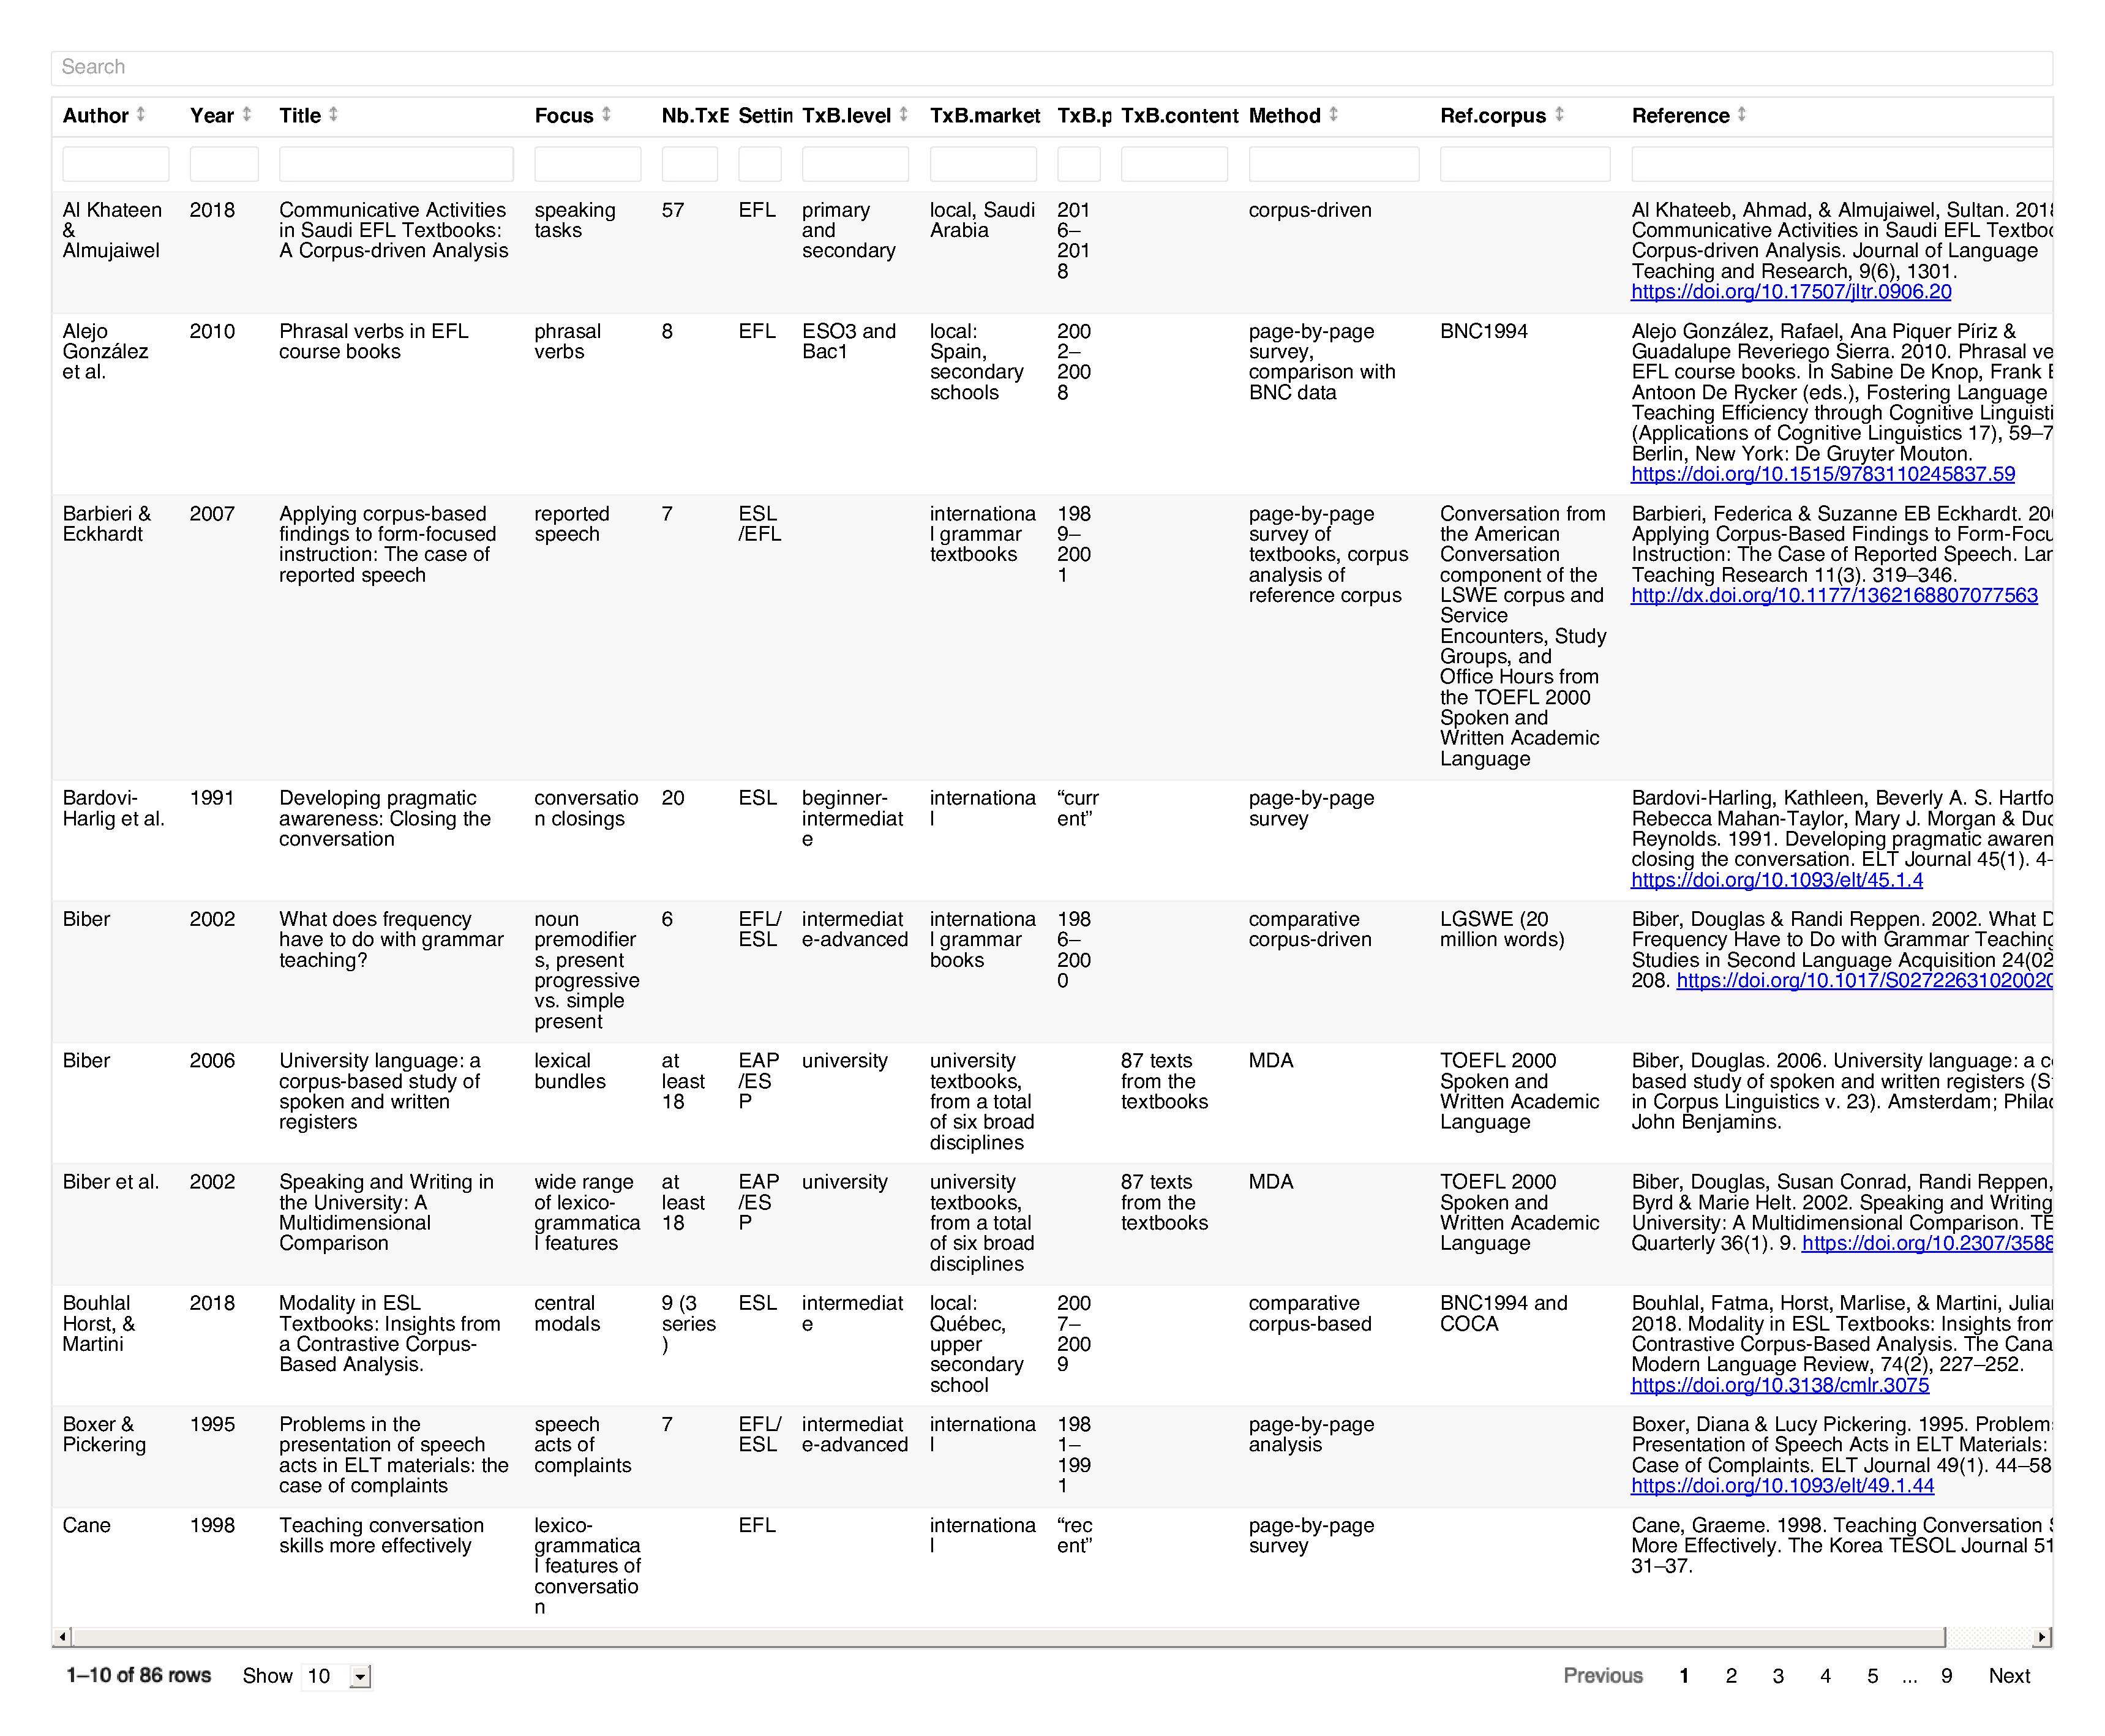
\includegraphics[keepaspectratio]{AppendixA_files/figure-pdf/display-1.pdf}}

The raw data can be downloaded as a comma-separated file from
\href{https://github.com/elenlefoll/TextbookMDA}{the project GitHub
repository}.

\chapter{Corpus Data}\label{corpus-data}

\section{Textbook English Corpus
(TEC)}\label{textbook-english-corpus-tec}

A detailed tabular overview of the composition of the Textbook English
Corpus (TEC) together with the full bibliographic metadata is available
at
\href{https://doi.org/10.5281/zenodo.4922819}{doi.org/10.5281/zenodo.4922819}.

Note that, for copyright reasons, the corpus itself cannot be published.
If you are interested in using the corpus for non-commercial research
purposes and/or in a potential research collaboration, please get in
touch with me via \href{https://orcid.org/0000-0002-5839-8010}{e-mail}.

\section{Reference corpora}\label{reference-corpora}

\subsection{Spoken BNC2014}\label{spoken-bnc2014}

The original corpus files of the Spoken British National Corpus (BNC)
2014 (Love et al. 2017; Love et al. 2019) can be downloaded for free for
research purposes from:
\url{http://corpora.lancs.ac.uk/bnc2014/signup.php}. I used the untagged
XML version.

The R script used to pre-process the untagged XML files into the format
used in this study (the ``John and Jill in Ivybridge'' version with
added full stops at speaker turns, as explained in Section 4.3.2.2 of
the book) can be found here:
\url{https://github.com/elenlefoll/TextbookEnglish/blob/main/3_Data/BNCspoken_nomark-up_JackJill.R}

\subsection{Informative Texts for Teens Corpus (Info
Teens)}\label{informative-texts-for-teens-corpus-info-teens}

For copyright reasons, the corpus itself cannot be made available.
Details of its composition can be found in Section 4.3.2.5 of the book.
If you are interested in using this corpus for non-commercial research
purposes and/or in a potential research collaboration, please get in
touch with me via \href{https://orcid.org/0000-0002-5839-8010}{e-mail}.

\subsection{Youth Fiction corpus}\label{youth-fiction-corpus}

For copyright reasons, the corpus itself cannot be made available. The
corresponding metadata can be found here:
\url{https://github.com/elenlefoll/TextbookEnglish/blob/main/3_Data/3_Youth_Fiction_Index.csv}.
If you are interested in using this corpus for non-commercial research
purposes and/or in a potential research collaboration, please get in
touch with me via \href{https://orcid.org/0000-0002-5839-8010}{e-mail}.

\chapter{Linguistic Features}\label{linguistic-features}

This table provides a tabular overview of the linguistic features tagged
by the MFTE Perl at the time of the data analysis.

For more information on the development of the tagger, see Le Foll
(2021b) and
\url{https://github.com/elenlefoll/MultiFeatureTaggerEnglish}.

\begin{tcolorbox}[enhanced jigsaw, toprule=.15mm, coltitle=black, rightrule=.15mm, colframe=quarto-callout-tip-color-frame, titlerule=0mm, bottomrule=.15mm, colbacktitle=quarto-callout-tip-color!10!white, colback=white, arc=.35mm, opacitybacktitle=0.6, toptitle=1mm, bottomtitle=1mm, leftrule=.75mm, left=2mm, title=\textcolor{quarto-callout-tip-color}{\faLightbulb}\hspace{0.5em}{Using the MFTE}, opacityback=0, breakable]

The Multi-Feature Tagger of English (MFTE) Perl is free to use and was
released under an Open Source licence. If you are interested in using
the MFTE for your own project, I recommend using the latest version of
the MFTE Python, which is much easier to use, can tag many more
features, and also underwent a thorough evaluation. Note also that all
future developments of the MFTE will be made on the MFTE Python. To find
out more, see Le Foll \& Shakir (2023) and
\url{https://github.com/mshakirDr/MFTE}.

\end{tcolorbox}

The following features were originally considered in this study. This
table is also available for download as a PDF at
\url{https://github.com/elenlefoll/MultiFeatureTaggerEnglish/blob/main/tables/ListFullMDAFeatures_3.1.pdf}.

\begin{table}[htbp]
\caption{}
\begin{tabular}{|l|l|l|l|l|l|l|}
\hline
\multicolumn{1}{|c|}{\textbf{Category}} & \multicolumn{1}{c|}{\textbf{Feature}} & \multicolumn{1}{c|}{\textbf{Code}} & \multicolumn{1}{c|}{\textbf{Examples}} & \multicolumn{1}{c|}{\textbf{                     Operationalisation                     }} & \multicolumn{1}{c|}{\textbf{Norm. unit}} & \multicolumn{1}{c|}{\textbf{As coded by}} \\ \hline
General text properties & Total number of words & \texttt{Words} & \textit{It's a shame that you'd have to pay to get that quality. (= 14)} & The number of tokens as tokenised by the Stanford Tagger, but excluding punctuation marks, brackets, symbols, genitive ‘s (POS), and filled pauses and interjections (FPUH). Contractions are treated as separate words, i.e., \textit{it's} is tokenised as \textit{it} and \textit{'s}. Note that this variable is only used to normalise the frequencies of other linguistic features. & NA & Le Foll \\ \hline
General text properties & Average word length & \texttt{AWL} & \textit{It's a shame that you'd have to pay to get that quality. (42/12 = 3.50)} & Total number of characters in a text divided by the number of words in that same text (as operationalised in the Words variable above, hence excluding filled pauses and interjections, cf. FPUH). & Words & Le Foll \\ \hline
General text properties & Lexical diversity & \texttt{TTR} & \textit{It's a shame that you'd have to pay to get that quality. (12/14 = 0.85)} & Following Biber (1988), this feature is a type-token ratio measured on the basis of, by default, the first 400 words of each text only. It is thus the number of unique word forms within the first 400 words of each text divided by 400. This number of words can be adjusted in the command used to run the script (see instructions at the top of the MFTE script). & Words (by default first 400) & Le Foll \\ \hline
General text properties & Lexical density & \texttt{LDE} & \textit{It's a shame that you'd have to pay to get that quality. (3/14 = 0.21)} & For this feature, tokens which are not on the list of the 352 function words from the {qdapDictionaries} R package, nor individual letters, or any of the fillers listed in FPUH are identified as content words. Lexical density is calculated as the ratio of these content words to the total number of words in a text. & Words & Le Foll \\ \hline
General text properties & Finite verbs & \texttt{--} & \textit{He discovered that the method involved imbiding copious amounts of tea. Ants can survive by joining together to morph into living rafts. Always wanted to experience the winter wonderland that Queen Elsa created?} & This feature is not directly listed in the MFTE output tables; however, it is used as a normalisation basis for many other linguistics features (see Normalisation column). It is calculated by tallying the number of occurrences of the following features: VPRT, VBD, VIMP, MDCA, MDCO, MDMM, MDNE, MDWO and MDWS. & NA & Le Foll \\ \hline
Adjectives & Attributive adjectives & \texttt{JJAT} & \textit{I’ve got a fantastic idea! I didn’t sleep at all last night. Cheap, quick and easy fix!} & Whereas the Biber Tagger and the MAT first identify predicative adjectives and then consider all remaining J.* tags from the Stanford Tagger to be attributive adjectives, the MFTE proceeds the other way around because it is considerably easier to reliably identify attributive adjectives than it is predicative adjectives. Thus, all adjectives (J.*, as tagged by the Stanford Tagger) followed by another adjective, a noun or a cardinal number, or preceded by a determiner are tagged as attributive adjectives. Once these first attributive adjectives have been identified, an additional loop is run to capture any additional attributive adjectives found in lists of attributive adjectives. & Nouns & Le Foll \\ \hline
Adjectives & Predicative adjectives & \texttt{JJPR} & \textit{That’s right. One of the main advantages of being famous... It must be absolutely wonderful.} & Once attributive adjectives have been identified (see JJAT) and tagged as JJAT, all remaining JJ, JJS and JJR tags are overwritten as JJPR. In addition, ok and okay in the construction \textit{BE ok(ay)} are also tagged as JJPR. These words are otherwise identified as foreign words (FW) by the Stanford Tagger.  & Finite verbs & Le Foll \\ \hline
Adverbials & Frequency references & \texttt{FREQ} & \textit{We should always wear a mask. But he had found his voice again.} & Assigned to all occurrences of the frequency adverbs listed in the COBUILD (Sinclair et al. 1900: 270): \textit{usually, always, mainly, often, generally, normally, traditionally, again, constantly, continually, frequently, ever, never, infrequently, intermittently, occasionally, often, periodically, rarely, regularly, repeatedly, seldom, sometimes} and \textit{sporadically}. & Finite verbs & Le Foll \\ \hline
Adverbials & Place references & \texttt{PLACE} & \textit{It’s not far to go. I’ll get it from upstairs. It’s downhill all the way. It’s there not here.} & Biber’s (1988: 224) list of place adverbials was taken from Quirk et al. (1985:514ff) but inexplicably excludes many from this list. Those that do not fulfil other major functions were therefore added: \textit{downwind, eastward(s), westward(s), northward(s), southward(s), upwards, downwards, elsewhere, everywhere, here, offshore, nowhere, somewhere, thereabout(s)} and \textit{there} (but occurrences of there tagged as existential \textit{there} (EX) by the Stanford Taggers were ignored). Only occurrences of far which have not previously identified as TIME references  (e.g., \textit{so far, thus far}) or emphatics  (e.g., \textit{far better, far more}) are tagged as PLACE references. & Finite verbs & Le Foll, adapted from Biber (1988) \\ \hline
Adverbials & Time references & \texttt{TIME} & \textit{It will soon be possible. Now is the time. I haven't come across any issues yet.} & All occurrences of \textit{afterwards, again, earlier, early, eventually, forever, formerly, immediately, initially, instantly, late, lately, later, momentarily, now, nowadays, once, originally, presently, previously, recently, shortly, simultaneously, subsequently, today, to-day, tomorrow, to-morrow, tonight, to-night, yesterday}. Following Nini (2014: 18), the word \textit{soon} was not tagged as a time adverbial when followed by the word \textit{as}. \textit{Ago, already, beforehand, prior to}, and \textit{far} (the latter only when proceeded by so or thus and not followed by an adjective or adverb), and \textit{am} and \textit{pm} as adverbs were added to the list, as well as \textit{yet} tokens that have not previously been identified as concessives (CONC). & Finite verbs & Le Foll, adapted from Nini (2014) \\ \hline
Adverbials & Other adverbs & \texttt{RB} & \textit{\textit{Unfortunately that’s the case. Exactly two weeks. He could so easily but he knows better. He’s still gonna come back.}} & Corresponds to all the tokens tagged as RB, RBS, RBR or WRB by the Stanford Tagger apart from those identified as adverbs of frequency (FREQ), place (PLACE) or time (TIME), amplifiers (AMP), emphatics (EMPH), hedges (HDG) and downtoners (DWNT). & Words & Le Foll \\ \hline
Determinatives & s-genitives & \texttt{POS} & \textit{the world’s two most populous country, my parents’ house} & As identified by the Stanford Tagger: the possessive endings on nouns ending in \textit{'s} or \textit{'}. Note that these tokens are not counted as Word in the computation of the lexical diversity (TTR) and average word length variables (AWL) features. & Nouns & Le Foll \\ \hline
Determinatives & Determiners & \texttt{DT} & \textit{Is that a new top? The first line has to be interesting. Are they both Spice Girls? On either side of the page. To another room. They’re five pounds each.} & As tagged by the Stanford Tagger (DT) (Santorini 1990: 2), with the exception of \textit{that, this, these} and \textit{those} which are counted as demonstratives (DEMO). Note that this Stanford Tagger category also includes pronouns such as another in \textit{Shall I choose another?} & Nouns & Le Foll \\ \hline
Determinatives & Quantifiers & \texttt{QUAN} & \textit{Such a good time in like half an hour. She’s got all these great ideas. It happens each and every time.} & All occurrences of pre-determiners as tagged by the Stanford Tagger, which includes the following "determiner-like elements when they precede an article or possessive pronoun" (Santorini 1990: 4): \textit{nary, quite, rather} and \textit{such} (e.g., \textit{quite a mess, rather a nuisance, many a moon}), as well as all instances of \textit{all} (unless immediately followed by \textit{right}, cf. DMA), \textit{any, a bit, both, each, every, few, half, many, much, several, some, lots, a lot (of), load(s) of, heaps of, wee, less} and \textit{more} (as adjectives only). & Nouns & Le Foll \\ \hline
Determinatives & Numbers & \texttt{CD} & \textit{That's her number one secret. Two eyes glowed just above the surface. It happened on 7 February, 2019.} & All cardinal numbers as identified by the Stanford Tagger. This includes dates written in numbers, e.g., \textit{1994}. In addition, numbers listed as list markers (LS) by the Stanford are overwritten as CD and specific combinations of digits and letters are also tagged as numbers (CD). & Words & Le Foll \\ \hline
Determinatives & Demonstratives & \texttt{DEMO} & \textit{What are you doing this weekend? I love that film. Whoever did that should admit it.} & Assigned to all occurrences of that, this, these and those identified by the Stanford Tagger as determiners (DT). & Words & Le Foll \\ \hline
Discourse organisation & Elaborating conjunctions & \texttt{ELAB} & \textit{Similarly, you may, for example, write bullet points insomuch as it helps you to focus your ideas.} & Assigned to \textit{such that} (not followed by a determiner), \textit{such as, inasmuch as, insofar as, insomuch as, in that, to the extent that, in particular, in conclusion, in sum, in summary, to summarise, to summarize, for example, for instance, in fact, in brief, in any event, in any case, in other words, e(.)g(.), in summary, viz(.), cf(.), i.e., namely, etc(.), likewise, namely}, as well as \textit{similarly} and \textit{accordingly} when followed by a comma. & Finite verbs & Le Foll \\ \hline
Discourse organisation & Coordinating conjunctions & \texttt{CC} & \textit{Instead of listening to us, he also told John and Jill but at least his parents don't know yet.} & \textit{This category takes the coordinating conjunctions (CC) tagged by the Stanford Tagger as its basis which include \textit{and, but, nor, or, yet}, "as well as the mathematical operators \textit{plus, minus, less, times} (in the sense of ‘multiplied by’) and \textit{over} (in the sense of ‘divided by’), when they are spelled out” (Santorini 1990: 2). However, conjunctions already captured by other variables are excluded from this count: \textit{yet} is assigned to concessive (CONC). In addition, the following (multi-word) conjunctions are also included in this category: \textit{also, besides, moreover, further} (when tagged as an adverb), \textit{furthermore, in addition, additionally, as well (as)} (except when preceded by least), \textit{however} (provided it is preceded or followed by a punctuation mark), \textit{ibid, on the one hand, on the other hand, instead, besides, conversely, by/in contrast, on the contrary, in/by comparison, whereas, whereby, whilst}.} & Finite verbs & Le Foll \\ \hline
Discourse organisation & Causal conjunctions & \texttt{CUZ} & \textit{He was scared because of the costume. Yeah coz he hated it.} & Assigned to all occurrences of \textit{because, 'cause, cos, cuz} and \textit{coz}. The latter four were not included in Biber’s (1988) original variable. According to Biber (1988: 236) because "is the only subordinator to function unambiguously as a causative adverbial". Whilst it is true that many subordinators, e.g., \textit{as, for}, and \textit{since}, can fulfil a range of functions, including causative, and were therefore not included in this category, the following adverbs and multi-word conjunctions were added since they mostly fulfil a causative function: \textit{as a result, on account of, for that/this purpose, thanks to, to that/this end, consequently, in consequence, hence, so that, therefore, thus}. & Finite verbs & Le Foll, adapted from Biber (1988) \\ \hline
Discourse organisation & Concessive conjunctions & \texttt{CONC} & \textit{Even though the antigens are normally hidden...} & Assigned to all occurrences of \textit{although, though, tho, despite, except that, in spite of, albeit, granted that, nevertheless, nonetheless, notwithstanding, whereas, no matter + WH-word, (ir)regardless of}, and \textit{granted}. Also assigned to \textit{still} and \textit{yet} when preceded by any punctuation mark or followed by a comma. Multi-word units are only counted as one occurrence of CONC. & Finite verbs & Le Foll \\ \hline
Discourse organisation & Conditional conjunctions & \texttt{COND} & \textit{If I were you... Even if the treatment works...} & Assigned to all occurrences of \textit{if, as long as, unless, lest, in that case, otherwise, whether}. & Finite verbs & Le Foll \\ \hline
Discourse organisation & Discourse/pragmatic markers & \texttt{DMA} & \textit{Well no they didn’t say actually. Okay I guess we’ll see how things go right?} & Assigned to "interactional signals and discourse markers" (as listed in Stenström 1994: 59 and cited in Aijmer 2002: 2): \textit{actually, all right, anyway, God, goodness, gosh, OK, okay, right} (if tagged as an interjection by the Stanford Tagger), \textit{well} (only if identified by the Stanford Tagger as an adverb or adjective and not if preceded by \textit{as, how, very, really, quite}, a verb, an adjective or an adverb), \textit{yes, yeah, yep, sure} (unless it is preceded by the verb \textit{MAKE, for, not} or \textit{you}). Verbal phrases such as \textit{you know} and \textit{I mean} were excluded from this variable since literal occurrences could not be automatically disambiguated occurrences as discourse markers. A number of markers from Stenström’s list are also not assigned this tag because they are captured by other variables: \textit{now} (TIME), \textit{please} (POLITE), \textit{really} (EMPH), \textit{quite} and \textit{sort of} (HDG). The following items were added: \textit{lol, IMO, omg, wtf, nope, mind you, of course, whatever} and \textit{damn} (unless tagged as a verb, or followed by an adjective; in the latter case it is an emphatic, cf. EMPH). & Words & Le Foll \\ \hline
Discourse organisation & Filled pauses and interjections & \texttt{FPUH} & \textit{Oh noooooo, Tiger’s furious! Wow! Hey Tom! Er I don’t know. Hmm.} & Assigned to all occurrences of \textit{ah+, aw+, oh+, eh+, er+, erm+, mm+, ow+, um+, huh+, uhu+, uhuh, mhm+, hm+} (but not HM), \textit{oo+ps woo+ps, hi, hey}, and interjections identified by the Stanford Tagger and not assigned to another category. The plus sign (+) signifies that that the preceding letter can appear multiple times, i.e., \textit{ahh} and \textit{errrr} are also assigned this tag. & Words & Le Foll \\ \hline
Discourse organisation & \textit{Like} & \texttt{LIKE} & \textit{Sounds like me. And just like his father. And he was like this isn’t true. I wasn’t gonna like do it.} & Occurrences of \textit{like} tagged as a preposition (IN) or adjective (JJ) by the Stanford Tagger are assigned this tag because, in spoken English, \textit{like} typically fulfils a range of different functions, e.g., fillers and softeners, and attempts to disambiguate like as a preposition or conjunct proved too error-prone. This category excludes occurrences of \textit{like} identified as the quotative \textit{BE + like} (QLIKE) if the QLIKE feature is included (which, by default, it is not, cf. tagger evaluation). & Words & Le Foll \\ \hline
Discourse organisation & \textit{So} & \texttt{SO} & \textit{She had spent so many summers there. So there you go.} & Occurrences of \textit{so} tagged as IN by the Stanford Tagger and not previously identified as either an emphatic (so + J.*/much/many/little; EMPH) or an adverbial subordinator (so that + NN.*/J.*; OSUB) are assigned this tag. & Words & Le Foll \\ \hline
Discourse organisation & Direct WH-questions & \texttt{WHQU} & \textit{What’s happening? Why don’t we call the game off? How? And who is Dinah, if I might venture to ask the question?} & Assigned to \textit{what, where, when, how, why, who, whom, whose} and \textit{which} followed by a question mark within 15 tokens. & Finite verbs & Le Foll \\ \hline
Discourse organisation & Question tags & \texttt{QUTAG} & \textit{Do they? Were you? It’s just it’s repetitive, isn’t it?} & Assigned to question marks preceded by (1) \textit{innit, init}; (2) a modal verb (MD) or \textit{did} or \textit{had}, and a personal pronoun (P.+); (3) a modal verb or \textit{did} or \textit{had}, a negation (XX0), and a personal pronoun; (4) \textit{is, does, was} or \textit{has}, followed by \textit{it, she} or \textit{he}; (5) \textit{is, does, was} or \textit{has}, followed by a negation, and \textit{it, she} or \textit{he}; (6) \textit{do, were, are} or \textit{have}, followed by \textit{you, we} or \textit{they}; (7) \textit{do, were, are} or \textit{have}, followed by a negation, and \textit{you, we} or \textit{they}. In addition, the above patterns are not considered question tags if a question word occurs within six words to the left of the question mark; consequently, \textit{Why did you do it?} is not assigned this tag but rather WHQU. & Finite verbs & Le Foll \\ \hline
Discourse organisation & Yes/no questions & \texttt{YNQU} & \textit{Have you thought about giving up? May I take a seat? Do you mind?} & Assigned to any form of the verbs \textit{BE, HAVE, DO} or a modal verb (MD) followed by a personal pronoun (P.+), a noun (NN.*), a negation (XX0) or determiner (DT) and then a question mark within three to 15 tokens, as long as no WH-question (WHQU) or \textit{yes/no} question tag (YNQU) is present one or two tokens before the auxiliary verb. Note that this variable should not overlap with question tags (QUTAG). & Finite verbs & Le Foll \\ \hline
Discourse organisation & that relative clauses & \texttt{THRC} & \textit{You must be very clever to find a use for something that costs nothing. I'll just run a cable that goes from here to there.} & Assigned to \textit{that} identified as introducing a relative clause by the Stanford Tagger (WDT), unless it is immediately followed by a punctuation mark. Any remaining \textit{that\_WDT} tokens are typically mistagged demonstratives and are thus assigned to the DEMO category, e.g., \textit{I don't think that's a problem that is}. & Finite verbs & Le Foll \\ \hline
Discourse organisation & \textit{that subordinate clauses (other than relatives)} & \texttt{THSC} & \textit{Did you know that the calendar we use today was started by Julius Caesar? She resented being told constantly that she was ignorant and stupid.} & Assigned to \textit{that} tokens which have been tagged as IN by the Stanford Tagger and are not immediately followed by a punctuation mark. Remaining \textit{\textit{that\_IN}} tokens are assigned to the demonstrative category (DEMO): these are end-of-sentences/utterances tokens which are typically misidentified by the Stanford Tagger, e.g., \textit{Who was that?} & Finite verbs & Le Foll \\ \hline
Discourse organisation & Subordinator that omission & \texttt{THATD} & \textit{I mean [THATD] you’ll do everything. I thought [THATD] he just meant our side. You don’t think [THATD] he’s a drug dealer? I know [THATD] that's not his thing.} & The THATD tag is assigned to the following patterns: (1) a public, private or suasive verb followed by a demonstrative pronoun (DEMO) or \textit{I, we, he, she, it, they} and then a verb (V.* or MD); (2) a public, private or suasive verb followed by \textit{I, we, he, she, it, they} or a \textit{noun} (N.*), and then by a verb (V.* or MD); (3) a public, private or suasive verb followed by an adjective (J.*), an adverb (RB), a determiner (DT, QUAN, CD) or a possessive pronoun (PRPS), and then a noun (N.*), and then a verb (V.* or MD), with the possibility of an intervening adjective (J.*) between the noun and its preceding word. This tag corresponds to Biber’s (1988: 244) category but its operationalisation has been improved to avoid the algorithm erroneously tagging constructions such as \textit{Why would I know that?} and \textit{He didn’t hear me thank God.} & Finite verbs & Le Foll, adapted from Biber (1988) \\ \hline
Discourse organisation & WH subordinate clauses & \texttt{WHSC} & \textit{I’m thinking of someone who is not here today. Do you know whether the banks are open?} & Assigned when the words \textit{what, where, when, how, whether, why, whoever, whomever, whichever, wherever} and \textit{whenever} have not been previously identified as part of a WH question (WHQU). Though many attempts were made, it proved impossible to reliably disambiguate between relative and other subordinate WH-clauses, which is why they are pooled together in this category. & Finite verbs & Le Foll \\ \hline
Lexis & Total nouns (including proper nouns) & \texttt{NN} & \textit{a cut, my coat, the findings, cruelty, comprehension, on Monday 6 Aug, the U.S., on the High Street} & Assigned to all singular (NN) and plural nouns (NNS) identified by the Stanford Tagger including proper nouns (NNP and NNPS). This variable differs from the Biber Tagger in that it includes nominalisations. & Words & Le Foll \\ \hline
Lexis & Noun compounds & \texttt{NCOMP} & \textit{Surely this stone must be the last one to cover the dungeon entrance! Experts say that the rare winter phenomenon is a natural occurrence.} & Assigned when two or more nouns follow each other without any intervening punctuation. The algorithm allows for the first noun to be a proper noun but not the second thus allowing for \textit{Monday afternoon} and \textit{Hollywood stars} but not \textit{Barack Obama} and \textit{Los Angeles}. It is also restricted to nouns with a minimum of two letters to avoid OCR errors (dots and images identified as individual letters and which are usually tagged as nouns by the Stanford Tagger) producing too many erroneous NCOMPs. Note that this feature works best with fully punctuated texts (see per-register recall and precision rates in the tagger documentation). & Nouns & Le Foll \\ \hline
Lexis & Emoji and emoticons & \texttt{EMO} & 😍 🥰 🌈 :-) :DD XD <3 :/ & Assigned to all emojis as of December 2018 (cf. https://unicode.org/emoji/charts/full-emoji-list.html) and to a range of emoticons, in particular three-character emoticons such as \textit{:-)}. The source code also includes three lines which are by default commented out but can be uncommented for texts where short emoticons are expected. It is not recommended to use these lines for general English because they lead to a sharp decrease in precision: many of the shorter emoticons, e.g., \textit{:( :D :3}, are too easy to confuse with poorly scanned texts that are missing spaces, or with the punctuation styles of specific academic journals.  & Words & Le Foll \\ \hline
Lexis & Hashtags & \texttt{HST} & \textit{\#phdlife \#Buy1Get1Free} & Assigned to any string starting with a hashtag followed by at least three letters, digits or underscores. & Words & Le Foll \\ \hline
Lexis & URL and e-mail addresses & \texttt{URL} & \textit{www.faz.net https://twitter.com elefoll@uos.de} & Assigned to all strings resembling a URL or an e-mail address (without claiming to only include valid URLs or e-mail addresses since this is not the aim). Regex for this feature was inspired by: https://mathiasbynens.be/demo/url-regex & Words & Le Foll \\ \hline
Negation & Negation & \texttt{XX0} & \textit{Why don’t you believe me? There is no way that’s happening any time soon. Nor am I.} & Biber’s (1988) analytic and synthetic negation features were merged into one negation variable since the latter is too infrequent to be of use in the context of this study. This unique negation tag is assigned to the tokens \textit{not\_RB, n’t\_RB}, all occurrences of the words nor and neither, and no when followed by an adjective (J.*) or noun (NN.*). & Finite verbs & Le Foll \\ \hline
Prepositions & Prepositions & \texttt{IN} & \textit{The Great Wall of China is the longest wall in the world. There are towers along the wall. I prefer to go to an art gallery. The objects on display are from all over the world.} & All items tagged as IN by the Stanford Tagger other than those assigned to CAUS, CONC, COND, OSUB, SO and LIKE.  & Words & Le Foll \\ \hline
Pronouns & Reference to the speaker/writer & \texttt{FPP1S} & \textit{I don’t know. It isn’t my problem.} & All occurrences of \textit{me, myself} and \textit{mine} and \textit{I} if tagged by the Stanford Tagger as a pronoun, a list symbol (LS), or a foreign word (FW). & Finite verbs & Le Foll \\ \hline
Pronouns & Reference to the speaker/writer and other(s) & \texttt{FPP1P} & \textit{We were told to deal with it ourselves.} & All occurrences of \textit{us, we, our, ourselves} and \textit{ours}, as well as the contracted form of \textit{us}  (e.g., in \textit{let’s}). All these terms are case insensitive but an exception for \textit{US} was added as this usually refers to the \textit{United States of America}. & Finite verbs & Le Foll \\ \hline
Pronouns & Reference to the addressee & \texttt{SPP2} & \textit{If your model was good enough, you’d be able to work it out.} & Following Biber (1988), all occurrences of \textit{you, your, yourself, yourselves}. Following Nini (2014: 18), also includes \textit{thy, thee} and \textit{thyself}. In addition, the forms \textit{ur, ye, y'all, ya, thine} and the nominal possessive pronoun \textit{yours} were also added. & Finite verbs & Le Foll, adapted from Nini (2014) \\ \hline
Pronouns & it pronoun reference & \texttt{PIT} & \textit{It fell and broke. I implemented it. Its impact has not yet been researched.} & All occurrences of the pronoun it. An exception was added for the all capital form \textit{IT} which most frequently refers to \textit{information technology}. Following Nini (2014: 18), also includes all occurrences of \textit{itself} and \textit{its}. & Finite verbs & Le Foll, adapted from Nini (2014) \\ \hline
Pronouns & One as a personal pronoun & \texttt{PRP} & \textit{One would hardly suppose that your eye was as steady as ever.} & This tag consists of the remaining personal pronouns not yet tagged as either first (FPP1S and FPP1P), second (SPP2) or third (TPP3) person pronouns. In practice, this should only leave \textit{one}. & Finite verbs & Le Foll \\ \hline
Pronouns & Reference to one non-interactant & \texttt{TPP3S} & \textit{He is beginning to form his own opinions. She does tend to keep to herself.} & Following Biber (1988), all occurrences of \textit{she, he, her, him, his, himself, herself} and \textit{themself}. Note that the singular \textit{they} form can only be accounted for with the possessive pronoun: \textit{themself}. & Finite verbs & Le Foll \\ \hline
Pronouns & Reference to more than one non-interactant & \texttt{TPP3P} & \textit{The text allows readers to grapple with their own conclusions. I wouldn't trust them.} & All occurrences of \textit{they, them, themselves, theirs} and \textit{em} when tagged by the Stanford Tagger as a pronoun. & Finite verbs & Le Foll \\ \hline
Pronouns & Quantifying pronouns & \texttt{QUPR} & \textit{said Alice aloud, addressing nobody in particular.} & All occurrences of \textit{anybody, anyone, anything, each other, everybody, everyone, everything, nobody, none, no one, nothing, somebody, someone} and \textit{something}. & Finite verbs & Nini (2014) \\ \hline
Stance-taking devices & Politeness markers & \texttt{POLITE} & \textit{Can you open the window, please? Would you mind giving me a hand? I was wondering whether you could help.} & Assigned to all occurrences of \textit{thanks, thank you, cheers, ta} (unless it is preceded by got to avoid the confusion with gotta), \textit{please, sorry, apology, apologies}, all forms of the verbs \textit{excuse, I/we wonder, I/we + BE + wondering}, and the n-grams \textit{you mind} and \textit{don’t mind}. No exception was made for \textit{please} as a verb because the Stanford Tagger frequently misidentifies please as a verb, e.g., \textit{I was like please\_VPRT just please\_VB just get there}. & Words & Le Foll \\ \hline
Stance-taking devices & Amplifiers & \texttt{AMP} & \textit{I am very tired. They were both thoroughly frightened.} & Assigned to the amplifiers from Biber’s (1988) list: \textit{absolutely, altogether, completely, enormously, entirely, extremely, fully, greatly, highly, intensely, perfectly, strongly, thoroughly, totally, utterly, very}. \textit{Especially} was added. & Words & Le Foll, adapted from Biber (1988) \\ \hline
Stance-taking devices & Downtoners & \texttt{DWNT} & \textit{These tickets were only 45 pounds. It’s almost time to go.} & Assigned to all occurrences of \textit{almost, barely, hardly, merely, mildly, nearly, only, partially, partly, practically, scarcely, slightly, somewhat}. In Biber (1988) almost is listed as both a hedge and a downtoner. Following Nini (2014), it is only considered a downtoner here. & Words & Nini (2014) \\ \hline
Stance-taking devices & Emphatics & \texttt{EMPH} & \textit{I do wish I hadn't drunk quite so much. Oh really? I just can’t get my head around it.} & Following Biber (1988), assigned to all occurrences of \textit{just, really, most, more, real + ADJ, so + ADJ, for sure, such a}. The algorithm was improved by adding \textit{so + much/little/many, such a/an} (whilst excluding such a/an if proceeded by of), and ensuring that only DO + verb in base form (VB) are tagged. Least and far + J.*/RB were added (the latter only when not proceeded by \textit{so} or \textit{thus}). To account for recent language change (Aijmer 2018), \textit{bloody, dead + ADJ, fucking} and \textit{super} were also added. Multi-word units are counted as one EMPH tag but several Words.  & Words & Le Foll, adapted from Biber (1988) \\ \hline
Stance-taking devices & Hedges & \texttt{HDG} & \textit{There seemed to be no sort of chance of getting out. I wish that kind of thing never happened. She's maybe gonna do it.} & Following Biber (1988: 240) assigned to all occurrences of \textit{maybe, at about, something like}, and \textit{more or less}, as well as \textit{sort of} and \textit{kind of} as long as they are not preceded by a determiner (DT), quantifier (QUAN), cardinal number (CD), adjective (J.*), possessive pronoun (PRPS) or WH-word. The condition that \textit{kind} must have been tagged as a noun (NN) by the Stanford Tagger was added to exclude phrases such as \textit{it’s very kind of you}. \textit{Kinda} and \textit{sorta} was added as colloquial alternatives to \textit{kind of} and \textit{sort of} and the adverbs \textit{apparently, conceivably, perhaps, possibly, presumably, probably, roughly} and \textit{somewhat} were also added to the list. & Words & Le Foll, adapted from Biber (1988) \\ \hline
Stative forms & Existential there & \texttt{EX} & \textit{There are students. And there is now a scholarship scheme.} & 
As tagged by the Stanford Tagger: “Existential there is the unstressed there that triggers inversion of the inflected verb and the logical subject of a sentence” (p. 3). & Finite verbs & Le Foll \\ \hline
Stative forms & Be as main verb & \texttt{BEMA} & \textit{It was nice to just be at home. She’s irreplaceable. It’s best I think. How was your mum on Sunday? It’s not long.} & Following Biber (1988), this tag is assigned to the all forms of the verb be when followed by a determiner (DT), a possessive pronoun (PRPS) a preposition (IN), or an adjective (JJ). In addition, Nini (2014: 20) improved the Biber Tagger “by taking into account that adverbs or negations can appear between the verb BE and the rest of the pattern. Furthermore, the algorithm was slightly modified and improved: (a) the problem of a double-coding of any existential \textit{there} followed by a form of BE as a BEMA was solved by imposing the condition that there should not appear immediately before or two before the pattern; (b) the cardinal numbers (CD) tag and the personal pronoun (PRP) tag were added to the list of items that can follow the form of BE.” This latter improvement by Nini, however, resulted in tag questions also being assigned to BEMA. The present algorithm therefore further excludes any occurrences of BE found one or two to the left of a question tag (QUTAG), as well as BE occurrences one or two to the left of a present participle form tagged as PROG or past participle form tagged as PASS. & Finite verbs & Le Foll, adapted from Nini (2014) \\ \hline
Syntax & Split auxiliaries and infinitives & \texttt{SPLIT} & \textit{I would actually drive. You can just so tell. I can’t ever imagine arguing with Jill. } & This category merges Biber’s (1988) split auxiliaries and split infinitive categories and follows Nini’s (2014: 30) operationalisations. Hence, this tag is assigned every time the infinitive marker \textit{to} (TO) is followed by one or two adverbs and a verb base form, and every time an auxiliary (any modal verb MD, or any form of DOAUX, or any form of BE, or any form of HAVE) is followed by one or two adverbs and a verb form. Nini's algorithm was improved to ensure that negated split auxiliaries would also be identified,  e.g., \textit{They have not yet published a patch}. & Finite verbs & Le Foll, adapted from Nini (2014) \\ \hline
Syntax & Stranded prepositions & \texttt{STPR} & \textit{We've got more than can be accounted for. Open the door and let them in. Where is it from? It's not the sort of music we're into.} & As in Biber (1988), assigned to the prepositions \textit{against, amid, amidst, among, amongst, at, between, by, despite, during, except, for, from, in, into, minus, of, off, on, onto, opposite, out, per, plus, pro, than, through, throughout, thru, toward, towards, upon, versus, via, with, within} and \textit{without} followed by any punctuation mark. Following Nini (2014: 30), besides was removed from Biber's original list since it also frequently serves as a conjunct and, in this function, is usually followed by a punctuation mark. Note that Nini's (2014:30) operationalisation tagged all occurrences of these word forms as prepositions regardless of how they were tagged by the Stanford Tagger. Here, it was decided to improve accuracy by restricting the query to tokens tagged as IN by the Stanford Tagger (thus excluding many RB and RP tokens, e.g., \textit{Don't take it away! Tie her up! He roared out: "Come away!"}). & Finite verbs & Le Foll, adapted from Nini (2014) \\ \hline
Verb features & Verbal contractions & \texttt{CONT} & \textit{I don’t know. It isn’t my problem. You’ll have to deal with it.} & Following (Nini 2014: 29), all occurrences of an apostrophe followed by a word identified as a verb (V.*, MD) by the Stanford Tagger and all occurrences of the token \textit{n’t\_XX0}. & Finite verbs & Nini (2014) \\ \hline
Verb features & Particles & \texttt{RP} & \textit{I’ll look it up. It’s coming down. When will you come over? Some of the birds hurried off at once.} & As tagged by the Stanford Tagger (RP) (Santorini 1990: 9-10). & Finite verbs & Le Foll \\ \hline
Verb features & BE-passives & \texttt{PASS} & \textit{He must have been burgled. They need to be informed. He was found out. When were they arrested?} & Assigned to past participles (here: VBN or VBD) preceded by the following patterns: 1) any form of the verb BE; 2) BE followed by one or two adverb(s) (RB) and/or a negation (XX0); 3) BE followed by a noun (NN.*) or personal pronoun (PRP); 4) BE followed by a noun (NN.*) or personal pronoun, and an adverb (RB) or negation (XX0). Unlike Biber (1988), no subdivision is made for by-passives and agentless passives. This choice is a) theoretically motivated because passives are too infrequent to be robustly measured at this level of granularity in most texts and b) for practical reasons because the algorithm proposed to identify by-passives resulted in too many false positives  (e.g.,  looking for things that have been made by hand). & Finite verbs & Le Foll \\ \hline
Verb features & GET-passives & \texttt{PGET} & \textit{He’s gonna get sacked. She’ll get me executed. It gets done all the time.} & Assigned to past participles (here: VBN or VBD) preceded by the following patterns: 1) any form of the verb GET; 2) GET followed by a noun (NN.*) or personal pronoun (PRP); 3) GET followed by a determiner (DT) or a noun (NN.*) plus a noun (NN.*). & Finite verbs & Le Foll \\ \hline
Verb features & Going to constructions & \texttt{GTO} & \textit{I’m not gonna go. You're going to absolutely love it there! Gonna come along?} & Assigned to all occurrences of \textit{going to} and \textit{gonna} followed by a base form verb (VB), allowing for up to one intervening word between \textit{going to} or \textit{gonna} and the infinitive. GTO constructions are excluded from the progressive (PROG) count. & Finite verbs & Le Foll \\ \hline
Verb features & Past tense & \texttt{VBD} & \textit{It fell and broke. I implemented it. If I were rich.} & As tagged by the Stanford Tagger, except where VBD tags are assumed to have been misassigned by the Stanford Tagger and are instead attributed to the perfect aspect (PEAS), passives (PASS, PGET) or USEDTO categories. & Finite verbs & Le Foll \\ \hline
Verb features & Non-finite verb -ing forms & \texttt{VBG} & \textit{He texted me saying no. He just started laughing. I remember thinking about that.} & All verb forms ending in -ing as tagged by the Stanford Tagger, except those identified as progressives (PROG) or going to constructions (GTO). This category also includes "putative prepositions" ending in \textit{-ing} such as \textit{according to} and \textit{concerning your request} (Santorini 1990: 11). & Finite verbs & Le Foll \\ \hline
Verb features & Non-finite -ed verb forms & \texttt{VBN} & \textit{These include cancers caused by viruses. Our content is grouped into sections called topics. Have you read any of the books mentioned in the blog?} & As tagged by the Stanford Tagger except for the exclusion of tokens identified as instances of the perfect aspect (PEAS), passives (PASS, PGET) and \textit{used to} constructions (USEDTO). Note that according to the Stanford Tagger rules, this category includes "putative prepositions" ending in \textit{-ed} such as \textit{granted that} and \textit{provided that} (Santorini 1990: 11). & Finite verbs & Le Foll \\ \hline
Verb features & Imperatives & \texttt{VIMP} & \textit{Let me know! Read the website and write the names of the characters. In groups, share your opinion. Always do as you're told!} & This tag is first assigned to any verb in base form (VB) occurring 1) immediately after a punctuation mark except a comma  (e.g.,  \textit{Okay: do it!}), an emoji or emoticon (EMO), a symbol (SYM), hashtag (HST), foreign word (FW) or a list marker (LS), or 2) after a punctuation mark and an adverb (e.g., \textit{1A. Then practice the dialogue}), unless the VB token is \textit{please} or \textit{thank} or has previously been identified as a DO auxiliary (DOAUX). In a second loop, the VIMP tag is assigned to VB verb tokens (except \textit{thank} or \textit{please}) when preceded by an imperative as identified above, with up to two optional intervening tokens, and the tokens \textit{and} or \textit{or} (e.g., \textit{Describe or draw, Listen carefully and repeat, Read the text and answer the questions}). In addition, a number of verbs frequently found in instructions are listed as exceptions (e.g., \textit{Complete, Choose, Check}) and are always assigned to this category when they are found at the beginning of a sentence regardless of their tag because these were found to be frequently erronouesly identified by the Stanford Tagger as nouns (NN). & Finite verbs & Le Foll \\ \hline
Verb features & Present tense & \texttt{VPRT} & \textit{It’s ours. Who doesn’t love it? I know.} & Subsumes the VBP (present tense other than third-person singular) and VBZ (third-person singular present tense) tags assigned by the Stanford Tagger. The MFTE also corrects systematic errors in the Stanford Tagger output by adding VPRT tags in strings such as \textit{I dunno} and \textit{there's}. & Finite verbs & Le Foll, adapted from Nini (2014) \\ \hline
Verb features & Perfect aspect & \texttt{PEAS} & \textit{Have you been on a student exchange? She’d already seen it. He has been told before. Is this the last novel you've read?} & Assigned to past participles (VBN, VBD) preceded by the following patterns: 1) any form of the verb HAVE; 2) HAVE followed by one or two adverb(s) (RB) and/or a negation (XX0); 3) HAVE followed by a noun (NN.*) or personal pronoun (PRP); 4) HAVE followed by a noun (NN.*) or personal pronoun, and an adverb (RB) or negation (XX0); 5) HAVE followed by a participle tagged as a passive (PASS); 6) HAVE followed by one or two adverb(s) (RB) and/or a negation (XX0), and a passive participle (PASS); 7) HAVE followed by a noun (NN.*) or personal pronoun (PRP), and a passive participle (PASS); 8) \textit{'s} as a verb (VBZ) followed by \textit{been, had, done} or a stative verb; 9) \textit{'s} as a verb (VBZ) followed by an adverb (RB) or negation (XX0), and \textit{been, had, done} or a stative verb (as listed under JJPR). & Finite verbs & Le Foll \\ \hline
Verb features & Progressive aspect & \texttt{PROG} & \textit{He wasn’t paying attention. I’m going to the market. I’m guessing you’re not going to be alone. I must be getting home.} & Assigned to any form of BE followed by an \textit{-ing} form of any verb (VBG). The algorithm allows for an intervening adverb (RB), emphatic (EMPH) and/or negation (XX0). The interrogative form is captured as BE followed by a noun (N.*) or personal pronoun (PRP) followed by the VBG token. As for the affirmative version, the latter algorithm also accounts for an intervening adverb (RB) and/or negation (XX0). \textit{Going to} constructions are excluded from this category and are tagged separately (GTO). & Finite verbs & Le Foll \\ \hline
Verb features & HAVE got constructions & \texttt{HGOT} & \textit{He’s got some. I haven’t got any.} & Assigned to the word got preceded by the following patterns: 1) any form of the verb HAVE; 2) HAVE followed by one or two adverb(s) (RB) and/or a negation (XX0); 3) HAVE followed by a noun (NN, NNP) or personal pronoun (PRP); 4) HAVE followed by a noun (NNP, NNP) or personal pronoun, and an adverb (RB) or negation (XX0). Note that this algorithm overwrites the perfect aspect (PEAS) and passive (PASS) tag. & Finite verbs & Le Foll \\ \hline
Verb semantics & DO auxiliary & \texttt{DOAUX} & \textit{Should take longer than it does. Ah you did. She needed that house, didn't she? You don’t really pay much attention, do you? Who did not already love him.} & Assigned to \textit{do, does} and \textit{did} as verbs in the following patterns: (a) when the next but one token is a base form verb (VB)  (e.g., \textit{did it work?, didn't hurt?}); (b) when the next but two token (+3) is a base form verb (VB)  (e.g., \textit{didn't it work}); (c) when it is immediately followed by an end-of-sentence punctuation mark  (e.g., \textit{you did?}); (d) when it is followed by a personal pronoun (PRP) or \textit{not} or \textit{n't} (XX0) and an end-of-sentence punctuation mark  (e.g., \textit{do you? He didn't!}); (e) when it is followed by \textit{not} or \textit{n't} (XX0) and a personal pronoun (PRP)  (e.g., \textit{didn't you?}); (f) when it is followed by a personal pronoun followed by any token and then a question mark  (e.g., \textit{did you really? did you not?}); (g) when it is preceded by a WH-question word. Additionally, all instances of DO immediately preceded by \textit{to} as an infinitive marker (TO) are excluded from this tag. & Finite verbs & Le Foll \\ \hline
Verb semantics & Activity verbs & \texttt{ACT} & \textit{I got up and ran out. Bring your CV. Where have you worked before? I go to school.} & Assigned to all forms of the verbs: \textit{buy, make, give, take, come, use, leave, show, try, work, move, follow, put, pay, bring, meet, play, run, hold, turn, send, sit, wait, walk, carry, lose, eat, watch, reach, add, produce, provide, pick, wear, open, win, catch, pass, shake, smile, stare, sell, spend, apply, form, obtain, arrange, beat, check, cover, divide, earn, extend, fix, hang, join, lie, obtain, pull, repeat, receive, save, share, smile, throw, visit, accompany, acquire, advance, behave, borrow, burn, clean, climb, combine, control, defend, deliver, dig, encounter, engage, exercise, expand, explore} and \textit{reduce} (cf. Biber 2006: 246, based on the LGSWE, pp. 361–362, 367–368, 370). Do is only included when it has not previously been tagged as an auxiliary (DOAUX). \textit{Get} and \textit{go} were removed from Biber’s (2006) list due to their high polysemy. Like Biber (2006), for practical reasons, no phrasal verbs were included in this variable. & Finite verbs & Le Foll, based on Biber (2006) \\ \hline
Verb semantics & Aspectual verbs & \texttt{ASPECT} & \textit{You should just keep talking. I started early today.} & Following Biber (2006: 247, based on the LGSWE, pp. 364, 369, 371), assigned to all forms of the verbs: \textit{start, keep, stop, begin, complete, end, finish, cease} and \textit{continue}. & Finite verbs & Biber 2006 \\ \hline
Verb semantics & Facilitation and causative verbs & \texttt{CAUSE} & \textit{He helped her escape. I pleaded with her to let me go.} & Following Biber (2006: 247, based on the LGSWE, pp. 363, 369, 370), assigned to all forms of the verbs: \textit{help, let, allow, affect, cause, enable, ensure, force, prevent, assist, guarantee, influence, permit} and \textit{require}. & Finite verbs & Biber 2006 \\ \hline
Verb semantics & Communication verbs & \texttt{COMM} & \textit{Describe it to your partner and say why. Write a list. Say what these words mean.} & Following Biber (2006: 247, based on the LGSWE, pp. 362, 368, 370), assigned to all forms of the verbs: \textit{say, tell, call, ask, write, talk, speak, thank, describe, claim, offer, admit, announce, answer, argue, deny, discuss, encourage, explain, express, insist, mention, offer, propose, quote, reply, shout, sign, sing, state, teach, warn, accuse, acknowledge, address, advise, appeal, assure, challenge, complain, consult, convince, declare, demand, emphasize, excuse, inform, invite, persuade, phone, pray, promise, question, recommend, remark, respond, specify, swear, threaten, urge, welcome, whisper and suggest. British spellings and the verbs agree, assert, beg, confide, command, disagree, object, pledge, pronounce, plead, report, testify, vow} and \textit{mean} were added. The latter was on Biber's (2006) list for mental verbs but, in most contexts encountered in the present study, it was found to be more likely to be a communication verb. & Finite verbs & Le Foll, based on Biber (2006) \\ \hline
Verb semantics & Existential or relationship verbs & \texttt{EXIST} & \textit{Weren’t they representing Jamaica? It encouraged young athletes to stay.} & Following Biber (2006: 247, based on the LGSWE, pp. 364, 369, 370–371), assigned to all forms of the verbs: \textit{seem, stand, stay, live, appear, include, involve, contain, exist, indicate, concern, constitute, define, derive, illustrate, imply, lack, owe, own, possess, suit, vary, deserve, fit, matter, reflect, relate, remain, reveal, sound, tend} and \textit{represent}. This variable does not include the copular BE. Look was removed from Biber’s original list because it frequently acts as an activity verb, too, e.g., \textit{I was looking for my glasses}. & Finite verbs & Le Foll, based on Biber (2006) \\ \hline
Verb semantics & Mental verbs & \texttt{MENTAL} & \textit{We want to see you tomorrow. Did you never hear back? I don’t recognize any.} & Following Biber (2006: 246-247, based on the LGSWE, pp. 362–363, 368–369, 370), assigned to all forms of the verbs: \textit{see, know, think, want, need} (unless identified as a necessity modal; cf. MDNE), \textit{feel, like, hear, remember, believe, read, consider, suppose, listen, love, wonder, understand, expect, hope, assume, determine, agree, bear, care, choose, compare, decide, discover, doubt, enjoy, examine, face, forget, hate, identify, imagine, intend, learn, mind, miss, notice, plan, prefer, prove, realize, recall, recognize, regard, suffer, wish, worry, accept, appreciate, approve, assess, blame, bother, calculate, conclude, celebrate, confirm, count, dare, detect, dismiss, distinguish, experience, fear, forgive, guess, ignore, impress, interpret, judge, justify, observe, perceive, predict, pretend, reckon, remind, satisfy, solve, study, suspect} and \textit{trust}. British spellings were added. \textit{Afford} and \textit{find}, which can be found on Biber's original list, were removed due to being too polysemous. Note that the phrase \textit{dunno}, which is incorrectly parsed by the Stanford Tagger, was also retagged as \textit{du\_VPRT n\_XX0 no\_VB} and \textit{that no\_VB} tokens are also assigned to this category. & Finite verbs & Le Foll, based on Biber (2006) \\ \hline
Verb semantics & Occurrence verbs & \texttt{OCCUR} & \textit{Couldn’t have happened at a busier time! The cricket lasts all day.} & Following Biber (2006: 247, based on the LGSWE pp. 364, 369, 370), assigned to all forms of the verbs: \textit{become, happen, change, die, grow, develop, arise, emerge, fall, increase, last, rise, disappear, flow, shine, sink, slip} and \textit{occur}. & Finite verbs & Biber 2006 \\ \hline
Verb semantics & Necessity modals & \texttt{MDNE} & \textit{I really must go. Shouldn’t you be going now? You need not have worried. Everybody needed to be needed.} & As in Biber (1988), all occurrences of \textit{ought, should} and \textit{must}. Contrary to Nini's operationalisation (2014: 27), only occurrences tagged as modals (MD) by the Stanford Tagger were included. In addition, \textit{need} when tagged as a modal by the Stanford Tagger (mostly when followed by \textit{not} or \textit{n't}) or when immediately followed by \textit{to} not tagged as a preposition (IN) was also added to this variable. & Finite verbs & Le Foll, adapted from Biber (1988) \\ \hline
Verb semantics & \textit{Modal can} & \texttt{MDCA} & \textit{Can I give him a hint? You cannot. I can't believe it! } & All occurrences of \textit{can} and \textit{ca} tagged as modals by the Stanford Tagger (MD). \textit{Ca} was included because the Stanford Tagger parses can't as \textit{ca + n't}. & Finite verbs & Le Foll \\ \hline
Verb semantics & \textit{Modal could} & \texttt{MDCO} & \textit{Do you think someone could have killed her? Well, that could be the problem. Could you do it by Friday?} & All occurrences of could tagged as a modal by the Stanford Tagger (MD).  & Finite verbs & Le Foll \\ \hline
Verb semantics & \textit{Modals may and might} & \texttt{MDMM} & \textit{May I have a word with you? But it might not be enough.} & All occurrences of \textit{may} and \textit{might} tagged as modals by the Stanford Tagger (MD).  & Finite verbs & Le Foll \\ \hline
Verb semantics & \textit{will and shall modals} & \texttt{MDWS} & \textit{It won’t do. Yes it will. Shall we see?} & The tokens \textit{will} and \textit{shall} and their contractions \textit{'ll, wo} and \textit{sha} when tagged as modals by the Stanford Tagger (MD). & Finite verbs & Le Foll \\ \hline
Verb semantics & \textit{modal would} & \texttt{MDWO} & \textit{Wouldn't you like to know? If I could afford to buy it I would. I'd like to think it works.} & The tokens \textit{will} and \textit{shall} and their contractions \textit{'ll, wo} and \textit{sha} when tagged as modals by the Stanford Tagger (MD). & Finite verbs & Le Foll \\ \hline
Verb semantics & \textit{be able to} & \texttt{ABLE} & \textit{It should be able to speak back to you. Would you be able to? } & Assigned to occurrences of the bigram \textit{(un)able to}, whenever \textit{(un)able} has previously been identified as a predicative adjective (JJPR). These occurrences of \textit{(un)able} are subsequently excluded from the JJPR count. & Finite verbs & Le Foll \\ \hline
Lexis & Foreign words & \texttt{FW} & \textit{I chose turkish delight and panna cotta. Merrry christmasss! Yo im gonna love it!} & All remaining words tagged by the Stanford Tagger as foreign words and not identified as other variables by the MFTE. Frequently includes words spelt with non-standard spellings, missing apostrophes, and poorly OCRed due to unusual fonts. Note that this feature is not counted by the MFTE. & NA & Stanford Tagger \\ \hline
Lexis & Symbols & \texttt{SYM} & \textit{\^a{} 2 EUR a go. I hope so \dagger{}. That's *all* they said!} & All remaining non alphanumeric tokens tagged by the Stanford Tagger as symbols (SYM) or list markers (LS) and not identified as other variables by the MFTE. Also frequently includes words poorly OCRed due to unusual fonts or poorly encoded text. Note that this feature is not counted by the MFTE. & -- & Stanford Tagger \\ \hline
Verb features & to-infinitives & \texttt{TO} & \textit{They were trying to find a solution. We like to think it’s doable. I went in there to kinda like celebrate.} & Following Nini (2014: 21), all occurrences of to except when followed by another \textit{\_IN token}, a number (CD), determiner (DT), adjective (J.*), possessive pronoun (PRPS), WH-word (WPS, WDT, WP, WRB), pre-determiner (PDT), noun (N.*) or pronoun (PRP). Note that, unlike Nini (2014), this feature is only used to identify other linguistic features. All occurrences of \textit{to} are counted as prepositions (IN) in the MFTE output tables. & -- & Nini (2014) \\ \hline
Verb features & Verb base form & \texttt{VB} & \textit{She would sit and read most afternoons. What do you use it for? Ask your parents to drive you to your friend's house.} & As tagged by the Stanford Tagger, except those identified as imperatives (VIMP). This feature is not included in the tables of counts outputted by the MFTE because it overlaps with other features (e.g., all the modal verb features). However, it is used to identify many other linguistic features. & -- & Le Foll \\ \hline
Verb semantics & Private verbs & -- & \textit{I don’t think this should be assumed. I suspect he can’t even remember it.} & As in Biber (1988, based on 1985: 1181), all forms of the verbs: \textit{accept, anticipate, ascertain, assume, believe, calculate, check, conclude, conjecture, consider, decide, deduce, deem, demonstrate, determine, discern, discover, doubt, dream, ensure, establish, estimate, expect, fancy, fear, feel, find, foresee, forget, gather, guess, hear, hold, hope, imagine, imply, indicate, infer, insure, judge, known, learn, mean, note, notice, observe, perceive, presume, presuppose, pretend, prove, realize, reason, recall, reckon, recognize, reflect, remember, reveal, see, sense, show, signify, suppose, suspect, think} and \textit{understand}. Note that this category is only used to identify that-omissions (THATD).  & -- & Biber 1988 \\ \hline
Verb semantics & Public verbs & NA & \textit{She promised she’d write back.} & As in Biber (1988, based on 1985: 1181), all forms of the verbs: \textit{acknowledge, add, admit, affirm, agree, allege, announce, argue, assert, bet, boast, certify, claim, comment, complain, concede, confess, confide, confirm, contend, convey, declare, deny, disclose, exclaim, explain, forecast, foretell, guarantee, hint, insist, maintain, mention, object, predict, proclaim, promise, pronounce, prophesy, protest, remark, repeat, reply, report, retort, say, state, submit, suggest, swear, testify, vow, warn} and \textit{write}. Note that this category is only used to identify that-omissions (THATD).  & NA & Le Foll, adapted from Biber (1988) \\ \hline
Verb semantics & Suasive verbs & -- & \textit{They were determined to make this work. I'd prefer to do it that way.} & As in Biber (1988, based on 1985: 1182–3), all forms of the verbs: \textit{agree, allow, arrange, ask, beg, command, concede, decide, decree, demand, desire, determine, enjoin, ensure, entreat, grant, insist, instruct, intend, move, ordain, order, pledge, pray, prefer, pronounce, propose, recommend, request, require, resolve, rule, stipulate, suggest, urge} and \textit{vote}. Note that this category is only used to identify that-omissions (THATD).  & NA & Biber 1988 \\ \hline
\end{tabular}
\label{}
\end{table}

\chapter{Evaluation of the Multi-Feature Tagger of English
(MFTE)}\label{evaluation-of-the-multi-feature-tagger-of-english-mfte}

For more information on the tagger itself, as well as the evaluation
data and methods, see Le Foll (2021b) and
\url{https://github.com/elenlefoll/MultiFeatureTaggerEnglish}.

\begin{tcolorbox}[enhanced jigsaw, toprule=.15mm, coltitle=black, rightrule=.15mm, colframe=quarto-callout-tip-color-frame, titlerule=0mm, bottomrule=.15mm, colbacktitle=quarto-callout-tip-color!10!white, colback=white, arc=.35mm, opacitybacktitle=0.6, toptitle=1mm, bottomtitle=1mm, leftrule=.75mm, left=2mm, title=\textcolor{quarto-callout-tip-color}{\faLightbulb}\hspace{0.5em}{Using the MFTE}, opacityback=0, breakable]

The Multi-Feature Tagger of English (MFTE) Perl is free to use and was
released under an Open Source licence. If you are interested in using
the MFTE for your own project, I recommend using the latest version of
the MFTE Python, which is much easier to use, can tag many more
features, and also underwent a thorough evaluation. Note also that all
future developments of the tool will be made on the MFTE Python. To find
out more, see Le Foll \& Shakir (2023) and
\url{https://github.com/mshakirDr/MFTE}.

\end{tcolorbox}

\section{Set-up}\label{set-up}

The following packages must be installed and loaded to process the
evaluation data.

\emph{Built with R 4.4.1}

\begin{Shaded}
\begin{Highlighting}[]
\CommentTok{\#renv::restore() \# Restore the project\textquotesingle{}s dependencies from the lockfile to ensure that same package versions are used as in the original thesis.}

\FunctionTok{library}\NormalTok{(caret) }\CommentTok{\# For computing confusion matrices}
\FunctionTok{library}\NormalTok{(harrypotter) }\CommentTok{\# Only for colour scheme}
\FunctionTok{library}\NormalTok{(here) }\CommentTok{\# For path management}
\FunctionTok{library}\NormalTok{(knitr) }\CommentTok{\# Loaded to display the tables using the kable() function}
\FunctionTok{library}\NormalTok{(paletteer) }\CommentTok{\# For nice colours}
\FunctionTok{library}\NormalTok{(readxl) }\CommentTok{\# For the direct import of Excel files}
\FunctionTok{library}\NormalTok{(tidyverse) }\CommentTok{\# For everything else!}
\end{Highlighting}
\end{Shaded}

\section{Data import from evaluation
files}\label{data-import-from-evaluation-files}

The data is imported directly from the Excel files in which the manual
tag check and corrections was performed. A number of data wrangling
steps need to be made for the data to be converted to a tidy format.

\begin{Shaded}
\begin{Highlighting}[]
\CommentTok{\# Function to import and wrangle the evaluation data from the Excel files in which the manual evaluation was conducted}
\NormalTok{importEval3 }\OtherTok{\textless{}{-}} \ControlFlowTok{function}\NormalTok{(file, fileID, register, corpus) \{}
\NormalTok{  Tag1 }\OtherTok{\textless{}{-}}\NormalTok{ file }\SpecialCharTok{|\textgreater{}} 
  \FunctionTok{add\_column}\NormalTok{(}\AttributeTok{FileID =}\NormalTok{ fileID, }\AttributeTok{Register =}\NormalTok{ register, }\AttributeTok{Corpus =}\NormalTok{ corpus) }\SpecialCharTok{|\textgreater{}}
  \FunctionTok{select}\NormalTok{(FileID, Corpus, Register, Output, Tokens, Tag1, Tag1Gold) }\SpecialCharTok{|\textgreater{}} 
  \FunctionTok{rename}\NormalTok{(}\AttributeTok{Tag =}\NormalTok{ Tag1, }\AttributeTok{TagGold =}\NormalTok{ Tag1Gold, }\AttributeTok{Token =}\NormalTok{ Tokens) }\SpecialCharTok{|\textgreater{}} 
  \FunctionTok{mutate}\NormalTok{(}\AttributeTok{Evaluation =} \FunctionTok{ifelse}\NormalTok{(}\FunctionTok{is.na}\NormalTok{(TagGold), }\ConstantTok{TRUE}\NormalTok{, }\ConstantTok{FALSE}\NormalTok{)) }\SpecialCharTok{|\textgreater{}} 
  \FunctionTok{mutate}\NormalTok{(}\AttributeTok{TagGold =} \FunctionTok{ifelse}\NormalTok{(}\FunctionTok{is.na}\NormalTok{(TagGold), }\FunctionTok{as.character}\NormalTok{(Tag), }\FunctionTok{as.character}\NormalTok{(TagGold))) }\SpecialCharTok{|\textgreater{}}
  \FunctionTok{filter}\NormalTok{(}\SpecialCharTok{!}\FunctionTok{is.na}\NormalTok{(Tag)) }\SpecialCharTok{|\textgreater{}} 
  \FunctionTok{mutate\_if}\NormalTok{(is.character, as.factor)}
  
\NormalTok{  Tag2 }\OtherTok{\textless{}{-}}\NormalTok{ file }\SpecialCharTok{|\textgreater{}} 
  \FunctionTok{add\_column}\NormalTok{(}\AttributeTok{FileID =}\NormalTok{ fileID, }\AttributeTok{Register =}\NormalTok{ register, }\AttributeTok{Corpus =}\NormalTok{ corpus) }\SpecialCharTok{|\textgreater{}}
  \FunctionTok{select}\NormalTok{(FileID, Corpus, Register, Output, Tokens, Tag2, Tag2Gold) }\SpecialCharTok{|\textgreater{}} 
  \FunctionTok{rename}\NormalTok{(}\AttributeTok{Tag =}\NormalTok{ Tag2, }\AttributeTok{TagGold =}\NormalTok{ Tag2Gold, }\AttributeTok{Token =}\NormalTok{ Tokens) }\SpecialCharTok{|\textgreater{}} 
  \FunctionTok{mutate}\NormalTok{(}\AttributeTok{Evaluation =} \FunctionTok{ifelse}\NormalTok{(}\FunctionTok{is.na}\NormalTok{(TagGold), }\ConstantTok{TRUE}\NormalTok{, }\ConstantTok{FALSE}\NormalTok{)) }\SpecialCharTok{|\textgreater{}} 
  \FunctionTok{mutate}\NormalTok{(}\AttributeTok{TagGold =} \FunctionTok{ifelse}\NormalTok{(}\FunctionTok{is.na}\NormalTok{(TagGold), }\FunctionTok{as.character}\NormalTok{(Tag), }\FunctionTok{as.character}\NormalTok{(TagGold))) }\SpecialCharTok{|\textgreater{}}
  \FunctionTok{filter}\NormalTok{(}\SpecialCharTok{!}\FunctionTok{is.na}\NormalTok{(Tag)) }\SpecialCharTok{|\textgreater{}} 
  \FunctionTok{mutate\_if}\NormalTok{(is.character, as.factor)}

\NormalTok{Tag3 }\OtherTok{\textless{}{-}}\NormalTok{ file }\SpecialCharTok{|\textgreater{}} 
  \FunctionTok{add\_column}\NormalTok{(}\AttributeTok{FileID =}\NormalTok{ fileID, }\AttributeTok{Register =}\NormalTok{ register, }\AttributeTok{Corpus =}\NormalTok{ corpus) }\SpecialCharTok{|\textgreater{}}
  \FunctionTok{select}\NormalTok{(FileID, Corpus, Register, Output, Tokens, Tag3, Tag3Gold) }\SpecialCharTok{|\textgreater{}} 
  \FunctionTok{rename}\NormalTok{(}\AttributeTok{Tag =}\NormalTok{ Tag3, }\AttributeTok{TagGold =}\NormalTok{ Tag3Gold, }\AttributeTok{Token =}\NormalTok{ Tokens) }\SpecialCharTok{|\textgreater{}} 
  \FunctionTok{mutate}\NormalTok{(}\AttributeTok{Evaluation =} \FunctionTok{ifelse}\NormalTok{(}\FunctionTok{is.na}\NormalTok{(TagGold), }\ConstantTok{TRUE}\NormalTok{, }\ConstantTok{FALSE}\NormalTok{)) }\SpecialCharTok{|\textgreater{}} 
  \FunctionTok{mutate}\NormalTok{(}\AttributeTok{TagGold =} \FunctionTok{ifelse}\NormalTok{(}\FunctionTok{is.na}\NormalTok{(TagGold), }\FunctionTok{as.character}\NormalTok{(Tag), }\FunctionTok{as.character}\NormalTok{(TagGold))) }\SpecialCharTok{|\textgreater{}}
  \FunctionTok{filter}\NormalTok{(}\SpecialCharTok{!}\FunctionTok{is.na}\NormalTok{(Tag)) }\SpecialCharTok{|\textgreater{}} 
  \FunctionTok{mutate\_if}\NormalTok{(is.character, as.factor)}

\NormalTok{output }\OtherTok{\textless{}{-}} \FunctionTok{rbind}\NormalTok{(Tag1, Tag2, Tag3) }\SpecialCharTok{|\textgreater{}} 
  \FunctionTok{mutate}\NormalTok{(}\FunctionTok{across}\NormalTok{(}\FunctionTok{where}\NormalTok{(is.factor), str\_remove\_all, }\AttributeTok{pattern =} \FunctionTok{fixed}\NormalTok{(}\StringTok{" "}\NormalTok{))) }\SpecialCharTok{|\textgreater{}} \CommentTok{\# Removes all white spaces which are found in the excel files}
  \FunctionTok{filter}\NormalTok{(}\SpecialCharTok{!}\FunctionTok{is.na}\NormalTok{(Output)) }\SpecialCharTok{|\textgreater{}} 
  \FunctionTok{mutate\_if}\NormalTok{(is.character, as.factor)}
\NormalTok{\}}

\CommentTok{\# Second function to import and wrangle the evaluation data for Excel files with four tag columns as opposed to three}
\NormalTok{importEval4 }\OtherTok{\textless{}{-}} \ControlFlowTok{function}\NormalTok{(file, fileID, register, corpus) \{}
\NormalTok{  Tag1 }\OtherTok{\textless{}{-}}\NormalTok{ file }\SpecialCharTok{|\textgreater{}} 
  \FunctionTok{add\_column}\NormalTok{(}\AttributeTok{FileID =}\NormalTok{ fileID, }\AttributeTok{Register =}\NormalTok{ register, }\AttributeTok{Corpus =}\NormalTok{ corpus) }\SpecialCharTok{|\textgreater{}}
  \FunctionTok{select}\NormalTok{(FileID, Corpus, Register, Output, Tokens, Tag1, Tag1Gold) }\SpecialCharTok{|\textgreater{}} 
  \FunctionTok{rename}\NormalTok{(}\AttributeTok{Tag =}\NormalTok{ Tag1, }\AttributeTok{TagGold =}\NormalTok{ Tag1Gold, }\AttributeTok{Token =}\NormalTok{ Tokens) }\SpecialCharTok{|\textgreater{}} 
  \FunctionTok{mutate}\NormalTok{(}\AttributeTok{Evaluation =} \FunctionTok{ifelse}\NormalTok{(}\FunctionTok{is.na}\NormalTok{(TagGold), }\ConstantTok{TRUE}\NormalTok{, }\ConstantTok{FALSE}\NormalTok{)) }\SpecialCharTok{|\textgreater{}} 
  \FunctionTok{mutate}\NormalTok{(}\AttributeTok{TagGold =} \FunctionTok{ifelse}\NormalTok{(}\FunctionTok{is.na}\NormalTok{(TagGold), }\FunctionTok{as.character}\NormalTok{(Tag), }\FunctionTok{as.character}\NormalTok{(TagGold))) }\SpecialCharTok{|\textgreater{}}
  \FunctionTok{filter}\NormalTok{(}\SpecialCharTok{!}\FunctionTok{is.na}\NormalTok{(Tag)) }\SpecialCharTok{|\textgreater{}} 
  \FunctionTok{mutate\_if}\NormalTok{(is.character, as.factor)}
  
\NormalTok{  Tag2 }\OtherTok{\textless{}{-}}\NormalTok{ file }\SpecialCharTok{|\textgreater{}} 
  \FunctionTok{add\_column}\NormalTok{(}\AttributeTok{FileID =}\NormalTok{ fileID, }\AttributeTok{Register =}\NormalTok{ register, }\AttributeTok{Corpus =}\NormalTok{ corpus) }\SpecialCharTok{|\textgreater{}}
  \FunctionTok{select}\NormalTok{(FileID, Corpus, Register, Output, Tokens, Tag2, Tag2Gold) }\SpecialCharTok{|\textgreater{}} 
  \FunctionTok{rename}\NormalTok{(}\AttributeTok{Tag =}\NormalTok{ Tag2, }\AttributeTok{TagGold =}\NormalTok{ Tag2Gold, }\AttributeTok{Token =}\NormalTok{ Tokens) }\SpecialCharTok{|\textgreater{}} 
  \FunctionTok{mutate}\NormalTok{(}\AttributeTok{Evaluation =} \FunctionTok{ifelse}\NormalTok{(}\FunctionTok{is.na}\NormalTok{(TagGold), }\ConstantTok{TRUE}\NormalTok{, }\ConstantTok{FALSE}\NormalTok{)) }\SpecialCharTok{|\textgreater{}} 
  \FunctionTok{mutate}\NormalTok{(}\AttributeTok{TagGold =} \FunctionTok{ifelse}\NormalTok{(}\FunctionTok{is.na}\NormalTok{(TagGold), }\FunctionTok{as.character}\NormalTok{(Tag), }\FunctionTok{as.character}\NormalTok{(TagGold))) }\SpecialCharTok{|\textgreater{}}
  \FunctionTok{filter}\NormalTok{(}\SpecialCharTok{!}\FunctionTok{is.na}\NormalTok{(Tag)) }\SpecialCharTok{|\textgreater{}} 
  \FunctionTok{mutate\_if}\NormalTok{(is.character, as.factor)}

\NormalTok{Tag3 }\OtherTok{\textless{}{-}}\NormalTok{ file }\SpecialCharTok{|\textgreater{}} 
  \FunctionTok{add\_column}\NormalTok{(}\AttributeTok{FileID =}\NormalTok{ fileID, }\AttributeTok{Register =}\NormalTok{ register, }\AttributeTok{Corpus =}\NormalTok{ corpus) }\SpecialCharTok{|\textgreater{}}
  \FunctionTok{select}\NormalTok{(FileID, Corpus, Register, Output, Tokens, Tag3, Tag3Gold) }\SpecialCharTok{|\textgreater{}} 
  \FunctionTok{rename}\NormalTok{(}\AttributeTok{Tag =}\NormalTok{ Tag3, }\AttributeTok{TagGold =}\NormalTok{ Tag3Gold, }\AttributeTok{Token =}\NormalTok{ Tokens) }\SpecialCharTok{|\textgreater{}} 
  \FunctionTok{mutate}\NormalTok{(}\AttributeTok{Evaluation =} \FunctionTok{ifelse}\NormalTok{(}\FunctionTok{is.na}\NormalTok{(TagGold), }\ConstantTok{TRUE}\NormalTok{, }\ConstantTok{FALSE}\NormalTok{)) }\SpecialCharTok{|\textgreater{}} 
  \FunctionTok{mutate}\NormalTok{(}\AttributeTok{TagGold =} \FunctionTok{ifelse}\NormalTok{(}\FunctionTok{is.na}\NormalTok{(TagGold), }\FunctionTok{as.character}\NormalTok{(Tag), }\FunctionTok{as.character}\NormalTok{(TagGold))) }\SpecialCharTok{|\textgreater{}}
  \FunctionTok{filter}\NormalTok{(}\SpecialCharTok{!}\FunctionTok{is.na}\NormalTok{(Tag)) }\SpecialCharTok{|\textgreater{}} 
  \FunctionTok{mutate\_if}\NormalTok{(is.character, as.factor)}

\NormalTok{Tag4 }\OtherTok{\textless{}{-}}\NormalTok{ file }\SpecialCharTok{|\textgreater{}} 
  \FunctionTok{add\_column}\NormalTok{(}\AttributeTok{FileID =}\NormalTok{ fileID, }\AttributeTok{Register =}\NormalTok{ register, }\AttributeTok{Corpus =}\NormalTok{ corpus) }\SpecialCharTok{|\textgreater{}}
  \FunctionTok{select}\NormalTok{(FileID, Corpus, Register, Output, Tokens, Tag4, Tag4Gold) }\SpecialCharTok{|\textgreater{}} 
  \FunctionTok{rename}\NormalTok{(}\AttributeTok{Tag =}\NormalTok{ Tag4, }\AttributeTok{TagGold =}\NormalTok{ Tag4Gold, }\AttributeTok{Token =}\NormalTok{ Tokens) }\SpecialCharTok{|\textgreater{}} 
  \FunctionTok{mutate}\NormalTok{(}\AttributeTok{Evaluation =} \FunctionTok{ifelse}\NormalTok{(}\FunctionTok{is.na}\NormalTok{(TagGold), }\ConstantTok{TRUE}\NormalTok{, }\ConstantTok{FALSE}\NormalTok{)) }\SpecialCharTok{|\textgreater{}} 
  \FunctionTok{mutate}\NormalTok{(}\AttributeTok{TagGold =} \FunctionTok{ifelse}\NormalTok{(}\FunctionTok{is.na}\NormalTok{(TagGold), }\FunctionTok{as.character}\NormalTok{(Tag), }\FunctionTok{as.character}\NormalTok{(TagGold))) }\SpecialCharTok{|\textgreater{}}
  \FunctionTok{filter}\NormalTok{(}\SpecialCharTok{!}\FunctionTok{is.na}\NormalTok{(Tag)) }\SpecialCharTok{|\textgreater{}} 
  \FunctionTok{mutate\_if}\NormalTok{(is.character, as.factor)}

\NormalTok{output }\OtherTok{\textless{}{-}} \FunctionTok{rbind}\NormalTok{(Tag1, Tag2, Tag3, Tag4) }\SpecialCharTok{|\textgreater{}} 
  \FunctionTok{mutate}\NormalTok{(}\FunctionTok{across}\NormalTok{(}\FunctionTok{where}\NormalTok{(is.factor), str\_remove\_all, }\AttributeTok{pattern =} \FunctionTok{fixed}\NormalTok{(}\StringTok{" "}\NormalTok{))) }\SpecialCharTok{|\textgreater{}} \CommentTok{\# Removes all white spaces which are found in the excel files}
  \FunctionTok{filter}\NormalTok{(}\SpecialCharTok{!}\FunctionTok{is.na}\NormalTok{(Tag)) }\SpecialCharTok{|\textgreater{}} 
  \FunctionTok{mutate\_if}\NormalTok{(is.character, as.factor)}

\NormalTok{\}}

\CommentTok{\# Function to decide which of the two above functions should be used}
\NormalTok{importEval }\OtherTok{\textless{}{-}} \ControlFlowTok{function}\NormalTok{(file, fileID, register, corpus) \{ }
  \ControlFlowTok{if}\NormalTok{(}\FunctionTok{sum}\NormalTok{(}\SpecialCharTok{!}\FunctionTok{is.na}\NormalTok{(file}\SpecialCharTok{$}\NormalTok{Tag4)) }\SpecialCharTok{\textgreater{}} \DecValTok{0}\NormalTok{) \{}
\NormalTok{    output }\OtherTok{=} \FunctionTok{importEval4}\NormalTok{(}\AttributeTok{file =}\NormalTok{ file, }\AttributeTok{fileID =}\NormalTok{ fileID, }\AttributeTok{register =}\NormalTok{ register, }\AttributeTok{corpus =}\NormalTok{ corpus)}
\NormalTok{  \}}
  \ControlFlowTok{else}\NormalTok{\{}
\NormalTok{    output }\OtherTok{=} \FunctionTok{importEval3}\NormalTok{(}\AttributeTok{file =}\NormalTok{ file, }\AttributeTok{fileID =}\NormalTok{ fileID, }\AttributeTok{register =}\NormalTok{ register, }\AttributeTok{corpus =}\NormalTok{ corpus)}
\NormalTok{  \}}
\NormalTok{\}}

\NormalTok{Solutions\_Intermediate\_Spoken\_0032 }\OtherTok{\textless{}{-}} \FunctionTok{importEval}\NormalTok{(}\AttributeTok{file =} \FunctionTok{read\_excel}\NormalTok{(}\FunctionTok{here}\NormalTok{(}\StringTok{"data"}\NormalTok{, }\StringTok{"MFTE"}\NormalTok{, }\StringTok{"evaluation"}\NormalTok{, }\StringTok{"Solutions\_Intermediate\_Spoken\_0032\_Evaluation.xlsx"}\NormalTok{)), }\AttributeTok{fileID =} \StringTok{"Solutions\_Intermediate\_Spoken\_0032"}\NormalTok{, }\AttributeTok{register =} \StringTok{"Conversation"}\NormalTok{, }\AttributeTok{corpus =} \StringTok{"TEC{-}Sp"}\NormalTok{)}

\NormalTok{HT\_5\_Poetry\_0001 }\OtherTok{\textless{}{-}} \FunctionTok{importEval}\NormalTok{(}\AttributeTok{file =} \FunctionTok{read\_excel}\NormalTok{(}\FunctionTok{here}\NormalTok{(}\StringTok{"data"}\NormalTok{, }\StringTok{"MFTE"}\NormalTok{, }\StringTok{"evaluation"}\NormalTok{, }\StringTok{"HT\_5\_Poetry\_0001\_Evaluation.xlsx"}\NormalTok{)), }\AttributeTok{fileID =} \StringTok{"HT\_5\_Poetry\_0001"}\NormalTok{, }\AttributeTok{register =} \StringTok{"Poetry"}\NormalTok{, }\AttributeTok{corpus =} \StringTok{"TEC{-}Fr"}\NormalTok{)}

\NormalTok{Achievers\_A1\_Informative\_0006 }\OtherTok{\textless{}{-}} \FunctionTok{importEval}\NormalTok{(}\AttributeTok{file =} \FunctionTok{read\_excel}\NormalTok{(}\FunctionTok{here}\NormalTok{(}\StringTok{"data"}\NormalTok{, }\StringTok{"MFTE"}\NormalTok{, }\StringTok{"evaluation"}\NormalTok{, }\StringTok{"Achievers\_A1\_Informative\_0006\_Evaluation.xlsx"}\NormalTok{)), }\AttributeTok{fileID =} \StringTok{"Achievers\_A1\_Informative\_0006"}\NormalTok{, }\AttributeTok{register =} \StringTok{"Informative"}\NormalTok{, }\AttributeTok{corpus =} \StringTok{"TEC{-}Sp"}\NormalTok{)}

\NormalTok{New\_GreenLine\_5\_Personal\_0003 }\OtherTok{\textless{}{-}} \FunctionTok{importEval}\NormalTok{(}\AttributeTok{file =} \FunctionTok{read\_excel}\NormalTok{(}\FunctionTok{here}\NormalTok{(}\StringTok{"data"}\NormalTok{, }\StringTok{"MFTE"}\NormalTok{, }\StringTok{"evaluation"}\NormalTok{, }\StringTok{"New\_GreenLine\_5\_Personal\_0003\_Evaluation.xlsx"}\NormalTok{)), }\AttributeTok{fileID =} \StringTok{"New\_GreenLine\_5\_Personal\_0003"}\NormalTok{, }\AttributeTok{register =} \StringTok{"Personal communication"}\NormalTok{, }\AttributeTok{corpus =} \StringTok{"TEC{-}Ger"}\NormalTok{)}

\NormalTok{Piece\_of\_cake\_3e\_Instructional\_0006 }\OtherTok{\textless{}{-}} \FunctionTok{importEval}\NormalTok{(}\AttributeTok{file =} \FunctionTok{read\_excel}\NormalTok{(}\FunctionTok{here}\NormalTok{(}\StringTok{"data"}\NormalTok{, }\StringTok{"MFTE"}\NormalTok{, }\StringTok{"evaluation"}\NormalTok{, }\StringTok{"Piece\_of\_cake\_3e\_Instructional\_0006\_Evaluation.xlsx"}\NormalTok{)), }\AttributeTok{fileID =} \StringTok{"Piece\_of\_cake\_3e\_Instructional\_0006"}\NormalTok{, }\AttributeTok{register =} \StringTok{"Instructional"}\NormalTok{, }\AttributeTok{corpus =} \StringTok{"TEC{-}Fr"}\NormalTok{)}

\NormalTok{Access\_4\_Narrative\_0006 }\OtherTok{\textless{}{-}} \FunctionTok{importEval}\NormalTok{(}\AttributeTok{file =} \FunctionTok{read\_excel}\NormalTok{(}\FunctionTok{here}\NormalTok{(}\StringTok{"data"}\NormalTok{, }\StringTok{"MFTE"}\NormalTok{, }\StringTok{"evaluation"}\NormalTok{, }\StringTok{"Access\_4\_Narrative\_0006\_Evaluation.xlsx"}\NormalTok{)), }\AttributeTok{fileID =} \StringTok{"Access\_4\_Narrative\_0006"}\NormalTok{, }\AttributeTok{register =} \StringTok{"Fiction"}\NormalTok{, }\AttributeTok{corpus =} \StringTok{"TEC{-}Ger"}\NormalTok{)}

\NormalTok{BNCBFict\_b2 }\OtherTok{\textless{}{-}} \FunctionTok{importEval}\NormalTok{(}\AttributeTok{file =} \FunctionTok{read\_excel}\NormalTok{(}\FunctionTok{here}\NormalTok{(}\StringTok{"data"}\NormalTok{, }\StringTok{"MFTE"}\NormalTok{, }\StringTok{"evaluation"}\NormalTok{, }\StringTok{"BNCBFict\_b2.xlsx"}\NormalTok{)), }\AttributeTok{fileID =} \StringTok{"BNCBFict\_b2"}\NormalTok{, }\AttributeTok{register =} \StringTok{"fiction"}\NormalTok{, }\AttributeTok{corpus =} \StringTok{"BNC2014"}\NormalTok{)}

\NormalTok{BNCBFict\_m54 }\OtherTok{\textless{}{-}} \FunctionTok{importEval}\NormalTok{(}\AttributeTok{file =} \FunctionTok{read\_excel}\NormalTok{(}\FunctionTok{here}\NormalTok{(}\StringTok{"data"}\NormalTok{, }\StringTok{"MFTE"}\NormalTok{, }\StringTok{"evaluation"}\NormalTok{, }\StringTok{"BNCBFict\_m54.xlsx"}\NormalTok{)), }\AttributeTok{fileID =} \StringTok{"BNCBFict\_m54"}\NormalTok{, }\AttributeTok{register =} \StringTok{"fiction"}\NormalTok{, }\AttributeTok{corpus =} \StringTok{"BNC2014"}\NormalTok{)}

\NormalTok{BNCBFict\_e27 }\OtherTok{\textless{}{-}} \FunctionTok{importEval}\NormalTok{(}\AttributeTok{file =} \FunctionTok{read\_excel}\NormalTok{(}\FunctionTok{here}\NormalTok{(}\StringTok{"data"}\NormalTok{, }\StringTok{"MFTE"}\NormalTok{, }\StringTok{"evaluation"}\NormalTok{, }\StringTok{"BNCBFict\_e27.xlsx"}\NormalTok{)), }\AttributeTok{fileID =} \StringTok{"BNCBFict\_e27"}\NormalTok{, }\AttributeTok{register =} \StringTok{"fiction"}\NormalTok{, }\AttributeTok{corpus =} \StringTok{"BNC2014"}\NormalTok{)}

\NormalTok{BNCBMass16 }\OtherTok{\textless{}{-}} \FunctionTok{importEval}\NormalTok{(}\AttributeTok{file =} \FunctionTok{read\_excel}\NormalTok{(}\FunctionTok{here}\NormalTok{(}\StringTok{"data"}\NormalTok{, }\StringTok{"MFTE"}\NormalTok{, }\StringTok{"evaluation"}\NormalTok{, }\StringTok{"BNCBMass16.xlsx"}\NormalTok{)), }\AttributeTok{fileID =} \StringTok{"BNCBMass16"}\NormalTok{, }\AttributeTok{register =} \StringTok{"news"}\NormalTok{, }\AttributeTok{corpus =} \StringTok{"BNC2014"}\NormalTok{)}

\NormalTok{BNCBMass23 }\OtherTok{\textless{}{-}} \FunctionTok{importEval}\NormalTok{(}\AttributeTok{file =} \FunctionTok{read\_excel}\NormalTok{(}\FunctionTok{here}\NormalTok{(}\StringTok{"data"}\NormalTok{, }\StringTok{"MFTE"}\NormalTok{, }\StringTok{"evaluation"}\NormalTok{, }\StringTok{"BNCBMass23.xlsx"}\NormalTok{)), }\AttributeTok{fileID =} \StringTok{"BNCBMass23"}\NormalTok{, }\AttributeTok{register =} \StringTok{"news"}\NormalTok{, }\AttributeTok{corpus =} \StringTok{"BNC2014"}\NormalTok{)}

\NormalTok{BNCBReg111 }\OtherTok{\textless{}{-}} \FunctionTok{importEval}\NormalTok{(}\AttributeTok{file =} \FunctionTok{read\_excel}\NormalTok{(}\FunctionTok{here}\NormalTok{(}\StringTok{"data"}\NormalTok{, }\StringTok{"MFTE"}\NormalTok{, }\StringTok{"evaluation"}\NormalTok{, }\StringTok{"BNCBReg111.xlsx"}\NormalTok{)), }\AttributeTok{fileID =} \StringTok{"BNCBReg111"}\NormalTok{, }\AttributeTok{register =} \StringTok{"news"}\NormalTok{, }\AttributeTok{corpus =} \StringTok{"BNC2014"}\NormalTok{)}

\NormalTok{BNCBReg750 }\OtherTok{\textless{}{-}} \FunctionTok{importEval}\NormalTok{(}\AttributeTok{file =} \FunctionTok{read\_excel}\NormalTok{(}\FunctionTok{here}\NormalTok{(}\StringTok{"data"}\NormalTok{, }\StringTok{"MFTE"}\NormalTok{, }\StringTok{"evaluation"}\NormalTok{, }\StringTok{"BNCBReg750.xlsx"}\NormalTok{)), }\AttributeTok{fileID =} \StringTok{"BNCBReg750"}\NormalTok{, }\AttributeTok{register =} \StringTok{"news"}\NormalTok{, }\AttributeTok{corpus =} \StringTok{"BNC2014"}\NormalTok{)}

\NormalTok{BNCBSer486 }\OtherTok{\textless{}{-}} \FunctionTok{importEval}\NormalTok{(}\AttributeTok{file =} \FunctionTok{read\_excel}\NormalTok{(}\FunctionTok{here}\NormalTok{(}\StringTok{"data"}\NormalTok{, }\StringTok{"MFTE"}\NormalTok{, }\StringTok{"evaluation"}\NormalTok{, }\StringTok{"BNCBSer486.xlsx"}\NormalTok{)), }\AttributeTok{fileID =} \StringTok{"BNCBSer486"}\NormalTok{, }\AttributeTok{register =} \StringTok{"news"}\NormalTok{, }\AttributeTok{corpus =} \StringTok{"BNC2014"}\NormalTok{)}

\NormalTok{BNCBSer562 }\OtherTok{\textless{}{-}} \FunctionTok{importEval}\NormalTok{(}\AttributeTok{file =} \FunctionTok{read\_excel}\NormalTok{(}\FunctionTok{here}\NormalTok{(}\StringTok{"data"}\NormalTok{, }\StringTok{"MFTE"}\NormalTok{, }\StringTok{"evaluation"}\NormalTok{, }\StringTok{"BNCBSer562.xlsx"}\NormalTok{)), }\AttributeTok{fileID =} \StringTok{"BNCBSer562"}\NormalTok{, }\AttributeTok{register =} \StringTok{"news"}\NormalTok{, }\AttributeTok{corpus =} \StringTok{"BNC2014"}\NormalTok{)}

\NormalTok{BNCBEBl8 }\OtherTok{\textless{}{-}} \FunctionTok{importEval}\NormalTok{(}\AttributeTok{file =} \FunctionTok{read\_excel}\NormalTok{(}\FunctionTok{here}\NormalTok{(}\StringTok{"data"}\NormalTok{, }\StringTok{"MFTE"}\NormalTok{, }\StringTok{"evaluation"}\NormalTok{, }\StringTok{"BNCBEBl8.xlsx"}\NormalTok{)), }\AttributeTok{fileID =} \StringTok{"BNCBEBl8"}\NormalTok{, }\AttributeTok{register =} \StringTok{"internet"}\NormalTok{, }\AttributeTok{corpus =} \StringTok{"BNC2014"}\NormalTok{)}

\NormalTok{BNCBEFor32 }\OtherTok{\textless{}{-}} \FunctionTok{importEval}\NormalTok{(}\AttributeTok{file =} \FunctionTok{read\_excel}\NormalTok{(}\FunctionTok{here}\NormalTok{(}\StringTok{"data"}\NormalTok{, }\StringTok{"MFTE"}\NormalTok{, }\StringTok{"evaluation"}\NormalTok{, }\StringTok{"BNCBEFor32.xlsx"}\NormalTok{)), }\AttributeTok{fileID =} \StringTok{"BNCBEFor32"}\NormalTok{, }\AttributeTok{register =} \StringTok{"internet"}\NormalTok{, }\AttributeTok{corpus =} \StringTok{"BNC2014"}\NormalTok{)}

\NormalTok{S2DD }\OtherTok{\textless{}{-}} \FunctionTok{importEval}\NormalTok{(}\AttributeTok{file =} \FunctionTok{read\_excel}\NormalTok{(}\FunctionTok{here}\NormalTok{(}\StringTok{"data"}\NormalTok{, }\StringTok{"MFTE"}\NormalTok{, }\StringTok{"evaluation"}\NormalTok{, }\StringTok{"S2DD.xlsx"}\NormalTok{)), }\AttributeTok{fileID =} \StringTok{"S2DD"}\NormalTok{, }\AttributeTok{register =} \StringTok{"spoken"}\NormalTok{, }\AttributeTok{corpus =} \StringTok{"BNC2014"}\NormalTok{)}

\NormalTok{S3AV }\OtherTok{\textless{}{-}} \FunctionTok{importEval}\NormalTok{(}\AttributeTok{file =} \FunctionTok{read\_excel}\NormalTok{(}\FunctionTok{here}\NormalTok{(}\StringTok{"data"}\NormalTok{, }\StringTok{"MFTE"}\NormalTok{, }\StringTok{"evaluation"}\NormalTok{, }\StringTok{"S3AV.xlsx"}\NormalTok{)), }\AttributeTok{fileID =} \StringTok{"S3AV"}\NormalTok{, }\AttributeTok{register =} \StringTok{"spoken"}\NormalTok{, }\AttributeTok{corpus =} \StringTok{"BNC2014"}\NormalTok{)}

\NormalTok{SEL5 }\OtherTok{\textless{}{-}} \FunctionTok{importEval}\NormalTok{(}\AttributeTok{file =} \FunctionTok{read\_excel}\NormalTok{(}\FunctionTok{here}\NormalTok{(}\StringTok{"data"}\NormalTok{, }\StringTok{"MFTE"}\NormalTok{, }\StringTok{"evaluation"}\NormalTok{, }\StringTok{"SEL5.xlsx"}\NormalTok{)), }\AttributeTok{fileID =} \StringTok{"SEL5"}\NormalTok{, }\AttributeTok{register =} \StringTok{"spoken"}\NormalTok{, }\AttributeTok{corpus =} \StringTok{"BNC2014"}\NormalTok{)}

\NormalTok{SVLK }\OtherTok{\textless{}{-}} \FunctionTok{importEval}\NormalTok{(}\AttributeTok{file =} \FunctionTok{read\_excel}\NormalTok{(}\FunctionTok{here}\NormalTok{(}\StringTok{"data"}\NormalTok{, }\StringTok{"MFTE"}\NormalTok{, }\StringTok{"evaluation"}\NormalTok{, }\StringTok{"SVLK.xlsx"}\NormalTok{)), }\AttributeTok{fileID =} \StringTok{"SVLK"}\NormalTok{, }\AttributeTok{register =} \StringTok{"spoken"}\NormalTok{, }\AttributeTok{corpus =} \StringTok{"BNC2014"}\NormalTok{)}

\NormalTok{SZXQ }\OtherTok{\textless{}{-}} \FunctionTok{importEval}\NormalTok{(}\AttributeTok{file =} \FunctionTok{read\_excel}\NormalTok{(}\FunctionTok{here}\NormalTok{(}\StringTok{"data"}\NormalTok{, }\StringTok{"MFTE"}\NormalTok{, }\StringTok{"evaluation"}\NormalTok{, }\StringTok{"SZXQ.xlsx"}\NormalTok{)), }\AttributeTok{fileID =} \StringTok{"SZXQ"}\NormalTok{, }\AttributeTok{register =} \StringTok{"spoken"}\NormalTok{, }\AttributeTok{corpus =} \StringTok{"BNC2014"}\NormalTok{)}

\NormalTok{TaggerEval }\OtherTok{\textless{}{-}} \FunctionTok{rbind}\NormalTok{(Solutions\_Intermediate\_Spoken\_0032, HT\_5\_Poetry\_0001, Achievers\_A1\_Informative\_0006, New\_GreenLine\_5\_Personal\_0003, Piece\_of\_cake\_3e\_Instructional\_0006, Access\_4\_Narrative\_0006, BNCBEBl8, BNCBFict\_b2, BNCBFict\_m54, BNCBFict\_e27, BNCBEFor32, BNCBMass16, BNCBMass23, BNCBReg111, BNCBReg750, BNCBSer486, BNCBSer562, S2DD, S3AV, SEL5, SVLK, SZXQ)}
\end{Highlighting}
\end{Shaded}

Some tags had to be merged to account for changes made to the MFTE
between the evaluation and the tagging of the corpora included in the
present study.

\begin{Shaded}
\begin{Highlighting}[]
\NormalTok{TaggerEval }\OtherTok{\textless{}{-}}\NormalTok{ TaggerEval }\SpecialCharTok{|\textgreater{}} 
  \FunctionTok{mutate}\NormalTok{(}\AttributeTok{Tag =} \FunctionTok{ifelse}\NormalTok{(Tag }\SpecialCharTok{==} \StringTok{"PHC"}\NormalTok{, }\StringTok{"CC"}\NormalTok{, }\FunctionTok{as.character}\NormalTok{(Tag))) }\SpecialCharTok{|\textgreater{}} 
  \FunctionTok{mutate}\NormalTok{(}\AttributeTok{TagGold =} \FunctionTok{ifelse}\NormalTok{(TagGold }\SpecialCharTok{==} \StringTok{"PHC"}\NormalTok{, }\StringTok{"CC"}\NormalTok{, }\FunctionTok{as.character}\NormalTok{(TagGold))) }\SpecialCharTok{|\textgreater{}} 
  \FunctionTok{mutate}\NormalTok{(}\AttributeTok{Tag =} \FunctionTok{ifelse}\NormalTok{(Tag }\SpecialCharTok{==} \StringTok{"QLIKE"}\NormalTok{, }\StringTok{"LIKE"}\NormalTok{, }\FunctionTok{as.character}\NormalTok{(Tag))) }\SpecialCharTok{|\textgreater{}} 
  \FunctionTok{mutate}\NormalTok{(}\AttributeTok{TagGold =} \FunctionTok{ifelse}\NormalTok{(TagGold }\SpecialCharTok{==} \StringTok{"QLIKE"}\NormalTok{, }\StringTok{"LIKE"}\NormalTok{, }\FunctionTok{as.character}\NormalTok{(TagGold))) }\SpecialCharTok{|\textgreater{}} 
  \FunctionTok{mutate}\NormalTok{(}\AttributeTok{Tag =} \FunctionTok{ifelse}\NormalTok{(Tag }\SpecialCharTok{==} \StringTok{"TO"}\NormalTok{, }\StringTok{"IN"}\NormalTok{, }\FunctionTok{as.character}\NormalTok{(Tag))) }\SpecialCharTok{|\textgreater{}} 
  \FunctionTok{mutate}\NormalTok{(}\AttributeTok{TagGold =} \FunctionTok{ifelse}\NormalTok{(TagGold }\SpecialCharTok{==} \StringTok{"TO"}\NormalTok{, }\StringTok{"IN"}\NormalTok{, }\FunctionTok{as.character}\NormalTok{(TagGold))) }\SpecialCharTok{|\textgreater{}} 
  \FunctionTok{mutate\_if}\NormalTok{(is.character, as.factor) }\SpecialCharTok{|\textgreater{}} 
  \FunctionTok{mutate}\NormalTok{(}\AttributeTok{Evaluation =} \FunctionTok{ifelse}\NormalTok{(}\FunctionTok{as.character}\NormalTok{(Tag) }\SpecialCharTok{==} \FunctionTok{as.character}\NormalTok{(TagGold), }\ConstantTok{TRUE}\NormalTok{, }\ConstantTok{FALSE}\NormalTok{))}

\CommentTok{\# head(TaggerEval) \# Check sanity of data}
\CommentTok{\# summary(TaggerEval) \# Check sanity of data}

\CommentTok{\# saveRDS(TaggerEval, here("data", "processed", "MFTE\_Evaluation\_Results.rds"))}

\CommentTok{\# write.csv(TaggerEval, here("data", "processed", "MFTE\_Evaluation\_Results.csv"))}
\end{Highlighting}
\end{Shaded}

This table provides a summary of the complete evaluation dataset. It
comprises 25,233 tags that were checked (and, if needs be, corrected) by
at least one human annotator. This number includes tags for punctuation
marks, which make up a considerable proportion of the tags.

\begin{verbatim}
          FileID          Corpus               Register        Output     
 BNCBFict_b2 : 2621   TEC-Sp : 1042   fiction      :6500   ._.    : 1156  
 BNCBFict_e27: 2104   TEC-Fr : 2058   news         :6312   the_DT :  820  
 BNCBFict_m54: 1775   TEC-Ger: 1415   spoken       :6047   ,_,    :  720  
 BNCBMass16  : 1619   BNC2014:20718   internet     :1859   a_DT   :  466  
 SEL5        : 1463                   Instructional:1048   of_IN  :  328  
 BNCBEFor32  : 1305                   Poetry       :1010   (Other):21742  
 (Other)     :14346                   (Other)      :2457   NA's   :    1  
     Token            Tag           TagGold      Evaluation     
 .      : 1156   NN     : 4415   NN     : 4328   Mode :logical  
 the    :  820   IN     : 2145   IN     : 2113   FALSE:832      
 ,      :  720   DT     : 1454   DT     : 1457   TRUE :24401    
 to     :  495   .      : 1367   .      : 1367                  
 's     :  493   VPRT   : 1044   VPRT   : 1054                  
 (Other):21547   VBD    :  899   VBD    :  895                  
 NA's   :    2   (Other):13909   (Other):14019                  
\end{verbatim}

\section{Estimating MFTE accuracy for Textbook
English}\label{estimating-mfte-accuracy-for-textbook-english}

In total, 4,515 tags from the TEC were manually checked. This chunk
calculates the recall and precision rates of each feature, ignoring all
punctuation and symbols.

\begin{Shaded}
\begin{Highlighting}[]
\NormalTok{data }\OtherTok{\textless{}{-}}\NormalTok{ TaggerEval }\SpecialCharTok{|\textgreater{}} 
  \FunctionTok{filter}\NormalTok{(Corpus }\SpecialCharTok{\%in\%} \FunctionTok{c}\NormalTok{(}\StringTok{"TEC{-}Fr"}\NormalTok{, }\StringTok{"TEC{-}Ger"}\NormalTok{, }\StringTok{"TEC{-}Sp"}\NormalTok{)) }\SpecialCharTok{|\textgreater{}} 
  \FunctionTok{filter}\NormalTok{(TagGold }\SpecialCharTok{!=} \StringTok{"UNCLEAR"}\NormalTok{) }\SpecialCharTok{|\textgreater{}} 
  \FunctionTok{filter}\NormalTok{(Tag }\SpecialCharTok{\%in\%} \FunctionTok{c}\NormalTok{(}\FunctionTok{str\_extract}\NormalTok{(Tag, }\StringTok{"[A{-}Z0{-}9]+"}\NormalTok{))) }\SpecialCharTok{|\textgreater{}} \CommentTok{\# Remove punctuation tags which are uninteresting here.}
  \FunctionTok{filter}\NormalTok{(Tag }\SpecialCharTok{!=} \StringTok{"SYM"} \SpecialCharTok{\&}\NormalTok{ Tag }\SpecialCharTok{!=} \StringTok{"\textasciigrave{}\textasciigrave{}"}\NormalTok{) }\SpecialCharTok{|\textgreater{}} 
  \FunctionTok{droplevels}\NormalTok{() }\SpecialCharTok{|\textgreater{}} 
  \FunctionTok{mutate}\NormalTok{(}\AttributeTok{Tag =} \FunctionTok{factor}\NormalTok{(Tag, }\AttributeTok{levels =} \FunctionTok{union}\NormalTok{(}\FunctionTok{levels}\NormalTok{(Tag), }\FunctionTok{levels}\NormalTok{(TagGold)))) }\SpecialCharTok{|\textgreater{}} \CommentTok{\# Ensure that the factor levels are the same for the next caret operation}
  \FunctionTok{mutate}\NormalTok{(}\AttributeTok{TagGold =} \FunctionTok{factor}\NormalTok{(TagGold, }\AttributeTok{levels =} \FunctionTok{union}\NormalTok{(}\FunctionTok{levels}\NormalTok{(Tag), }\FunctionTok{levels}\NormalTok{(TagGold))))}

\CommentTok{\# Spot gold tag corrections that are not actually errors (should return zero rows if all is well)}
\CommentTok{\# data[data$Tag==data$TagGold \& data$Evaluation == FALSE,] |\textgreater{} as.data.frame()}
\end{Highlighting}
\end{Shaded}

The breakdown of inaccurate vs.~accurate tags in this TEC evaluation
sample is:

\begin{verbatim}
   Mode   FALSE    TRUE 
logical     114    3831 
\end{verbatim}

Note that the following accuracy metrics calculated using the
\texttt{caret::confusionMatrix} are not very representative because they
include tags, which were not entered in the study, e.g., LS and FW.

\begin{verbatim}
      Accuracy          Kappa  AccuracyLower  AccuracyUpper   AccuracyNull 
          0.97           0.97           0.97           0.98           0.20 
AccuracyPValue  McnemarPValue 
          0.00            NaN 
\end{verbatim}

Accuracy metrics per feature are more interesting and relevant.

\begin{longtable}[]{@{}lrrr@{}}
\toprule\noalign{}
& Precision & Recall & F1 \\
\midrule\noalign{}
\endhead
\bottomrule\noalign{}
\endlastfoot
Class: ABLE & 1.00 & 1.00 & 1.00 \\
Class: ACT & 0.97 & 0.98 & 0.98 \\
Class: AMP & 1.00 & 1.00 & 1.00 \\
Class: ASPECT & 1.00 & 1.00 & 1.00 \\
Class: BEMA & 1.00 & 1.00 & 1.00 \\
Class: CAUSE & 1.00 & 1.00 & 1.00 \\
Class: CC & 1.00 & 0.99 & 1.00 \\
Class: CD & 0.95 & 0.95 & 0.95 \\
Class: COMM & 1.00 & 0.98 & 0.99 \\
Class: COND & 1.00 & 1.00 & 1.00 \\
Class: CONT & 1.00 & 1.00 & 1.00 \\
Class: CUZ & 1.00 & 1.00 & 1.00 \\
Class: DEMO & 0.97 & 0.97 & 0.97 \\
Class: DMA & 1.00 & 1.00 & 1.00 \\
Class: DOAUX & 0.86 & 1.00 & 0.92 \\
Class: DT & 1.00 & 1.00 & 1.00 \\
Class: DWNT & 0.67 & 1.00 & 0.80 \\
Class: ELAB & 1.00 & 1.00 & 1.00 \\
Class: EMPH & 0.83 & 1.00 & 0.91 \\
Class: EX & 1.00 & 1.00 & 1.00 \\
Class: EXIST & 1.00 & 1.00 & 1.00 \\
Class: FPP1P & 1.00 & 1.00 & 1.00 \\
Class: FPP1S & 1.00 & 1.00 & 1.00 \\
Class: FPUH & 1.00 & 1.00 & 1.00 \\
Class: FREQ & 1.00 & 1.00 & 1.00 \\
Class: FW & 0.10 & 1.00 & 0.18 \\
Class: GTO & 1.00 & 1.00 & 1.00 \\
Class: HDG & 1.00 & 1.00 & 1.00 \\
Class: HGOT & 1.00 & 1.00 & 1.00 \\
Class: IN & 1.00 & 1.00 & 1.00 \\
Class: JJ & 0.96 & 0.98 & 0.97 \\
Class: JPRED & 0.97 & 0.90 & 0.94 \\
Class: LIKE & 0.83 & 1.00 & 0.91 \\
Class: MDCA & 1.00 & 1.00 & 1.00 \\
Class: MDCO & 1.00 & 1.00 & 1.00 \\
Class: MDMM & 1.00 & 0.67 & 0.80 \\
Class: MDNE & 1.00 & 0.80 & 0.89 \\
Class: MDWO & 1.00 & 1.00 & 1.00 \\
Class: MDWS & 1.00 & 1.00 & 1.00 \\
Class: MENTAL & 0.99 & 0.99 & 0.99 \\
Class: NCOMP & 0.88 & 1.00 & 0.94 \\
Class: NN & 0.95 & 0.99 & 0.97 \\
Class: NULL & 1.00 & 0.08 & 0.14 \\
Class: OCCUR & 0.94 & 1.00 & 0.97 \\
Class: PASS & 0.89 & 0.89 & 0.89 \\
Class: PEAS & 1.00 & 0.87 & 0.93 \\
Class: PGET & 1.00 & 1.00 & 1.00 \\
Class: PIT & 1.00 & 1.00 & 1.00 \\
Class: PLACE & 1.00 & 0.83 & 0.91 \\
Class: POLITE & 1.00 & 1.00 & 1.00 \\
Class: POS & 1.00 & 1.00 & 1.00 \\
Class: PROG & 1.00 & 0.89 & 0.94 \\
Class: QUAN & 0.96 & 0.98 & 0.97 \\
Class: QUPR & 1.00 & 1.00 & 1.00 \\
Class: RB & 1.00 & 0.99 & 0.99 \\
Class: RP & 1.00 & 1.00 & 1.00 \\
Class: SO & 1.00 & 0.64 & 0.78 \\
Class: SPLIT & 1.00 & 1.00 & 1.00 \\
Class: SPP2 & 1.00 & 1.00 & 1.00 \\
Class: STPR & 0.60 & 1.00 & 0.75 \\
Class: THATD & 0.86 & 1.00 & 0.92 \\
Class: THRC & 1.00 & 0.71 & 0.83 \\
Class: THSC & 0.69 & 1.00 & 0.82 \\
Class: TIME & 1.00 & 0.97 & 0.98 \\
Class: TPP3P & 1.00 & 1.00 & 1.00 \\
Class: TPP3S & 1.00 & 1.00 & 1.00 \\
Class: VB & 0.94 & 0.94 & 0.94 \\
Class: VBD & 0.97 & 0.99 & 0.98 \\
Class: VBG & 0.96 & 1.00 & 0.98 \\
Class: VBN & 0.85 & 0.92 & 0.88 \\
Class: VIMP & 0.99 & 0.88 & 0.93 \\
Class: VPRT & 0.98 & 0.98 & 0.98 \\
Class: WHQU & 0.97 & 1.00 & 0.98 \\
Class: WHSC & 1.00 & 0.97 & 0.99 \\
Class: XX0 & 1.00 & 1.00 & 1.00 \\
Class: YNQU & 1.00 & 1.00 & 1.00 \\
Class: OCR & NA & 0.00 & NA \\
\end{longtable}

\section{MFTE accuracy for reference corpora (or comparable
corpora)}\label{mfte-accuracy-for-reference-corpora-or-comparable-corpora}

\subsection{Conversation}\label{conversation}

These are extracts from the Spoken BNC2014 (as entered in the study).
The evaluation data for this sample excludes 7 tokens deemed
\emph{unclear} by at least one human annotator.

\begin{Shaded}
\begin{Highlighting}[]
\NormalTok{data }\OtherTok{\textless{}{-}}\NormalTok{ TaggerEval }\SpecialCharTok{|\textgreater{}} 
  \FunctionTok{filter}\NormalTok{(Register }\SpecialCharTok{==} \StringTok{"spoken"}\NormalTok{) }\SpecialCharTok{|\textgreater{}} 
  \FunctionTok{filter}\NormalTok{(TagGold }\SpecialCharTok{!=} \StringTok{"UNCLEAR"}\NormalTok{) }\SpecialCharTok{|\textgreater{}} 
  \FunctionTok{filter}\NormalTok{(Tag }\SpecialCharTok{\%in\%} \FunctionTok{c}\NormalTok{(}\FunctionTok{str\_extract}\NormalTok{(Tag, }\StringTok{"[A{-}Z0{-}9]+"}\NormalTok{))) }\SpecialCharTok{|\textgreater{}} \CommentTok{\# Remove all punctuation tags which are uninteresting here.}
  \FunctionTok{droplevels}\NormalTok{() }\SpecialCharTok{|\textgreater{}} 
  \FunctionTok{mutate}\NormalTok{(}\AttributeTok{Tag =} \FunctionTok{factor}\NormalTok{(Tag, }\AttributeTok{levels =} \FunctionTok{union}\NormalTok{(}\FunctionTok{levels}\NormalTok{(Tag), }\FunctionTok{levels}\NormalTok{(TagGold)))) }\SpecialCharTok{|\textgreater{}} \CommentTok{\# Ensure that the factor levels are the same for the next caret operation}
  \FunctionTok{mutate}\NormalTok{(}\AttributeTok{TagGold =} \FunctionTok{factor}\NormalTok{(TagGold, }\AttributeTok{levels =} \FunctionTok{union}\NormalTok{(}\FunctionTok{levels}\NormalTok{(Tag), }\FunctionTok{levels}\NormalTok{(TagGold))))}

\CommentTok{\# Spot gold tag corrections that are not actually errors (should return zero rows if all is well)}
\CommentTok{\# data[data$Tag==data$TagGold \& data$Evaluation == FALSE,] |\textgreater{} as.data.frame()}
\end{Highlighting}
\end{Shaded}

The breakdown of inaccurate vs.~accurate tags in this evaluation sample
is:

\begin{verbatim}
   Mode   FALSE    TRUE 
logical     224    5388 
\end{verbatim}

Note that the following accuracy metrics calculated using the
\texttt{caret::confusionMatrix} are not very representative because they
include tags, which were not entered in the study, e.g., LS and FW.

\begin{verbatim}
      Accuracy          Kappa  AccuracyLower  AccuracyUpper   AccuracyNull 
          0.96           0.96           0.95           0.97           0.12 
AccuracyPValue  McnemarPValue 
          0.00            NaN 
\end{verbatim}

\subsection{Fiction}\label{fiction}

The evaluation data for this sample excludes 0 tokens deemed
\emph{unclear} by at least one human annotator.

\begin{Shaded}
\begin{Highlighting}[]
\NormalTok{data }\OtherTok{\textless{}{-}}\NormalTok{ TaggerEval }\SpecialCharTok{|\textgreater{}} 
  \FunctionTok{filter}\NormalTok{(Register }\SpecialCharTok{==} \StringTok{"fiction"}\NormalTok{) }\SpecialCharTok{|\textgreater{}} 
  \FunctionTok{filter}\NormalTok{(TagGold }\SpecialCharTok{!=} \StringTok{"UNCLEAR"}\NormalTok{) }\SpecialCharTok{|\textgreater{}} 
  \FunctionTok{filter}\NormalTok{(Tag }\SpecialCharTok{\%in\%} \FunctionTok{c}\NormalTok{(}\FunctionTok{str\_extract}\NormalTok{(Tag, }\StringTok{"[A{-}Z0{-}9]+"}\NormalTok{))) }\SpecialCharTok{|\textgreater{}} \CommentTok{\# Remove all punctuation tags which are uninteresting here.}
  \FunctionTok{filter}\NormalTok{(Tag }\SpecialCharTok{!=} \StringTok{"SYM"} \SpecialCharTok{\&}\NormalTok{ Tag }\SpecialCharTok{!=} \StringTok{"\textasciigrave{}\textasciigrave{}"}\NormalTok{) }\SpecialCharTok{|\textgreater{}} 
  \FunctionTok{droplevels}\NormalTok{() }\SpecialCharTok{|\textgreater{}} 
  \FunctionTok{mutate}\NormalTok{(}\AttributeTok{Tag =} \FunctionTok{factor}\NormalTok{(Tag, }\AttributeTok{levels =} \FunctionTok{union}\NormalTok{(}\FunctionTok{levels}\NormalTok{(Tag), }\FunctionTok{levels}\NormalTok{(TagGold)))) }\SpecialCharTok{|\textgreater{}} \CommentTok{\# Ensure that the factor levels are the same for the next caret operation}
  \FunctionTok{mutate}\NormalTok{(}\AttributeTok{TagGold =} \FunctionTok{factor}\NormalTok{(TagGold, }\AttributeTok{levels =} \FunctionTok{union}\NormalTok{(}\FunctionTok{levels}\NormalTok{(Tag), }\FunctionTok{levels}\NormalTok{(TagGold))))}

\CommentTok{\# Spot gold tag corrections that are not actually errors (should return zero rows if all is well)}
\CommentTok{\# data[data$Tag==data$TagGold \& data$Evaluation == FALSE,] |\textgreater{} as.data.frame()}
\end{Highlighting}
\end{Shaded}

The breakdown of inaccurate vs.~accurate tags in this evaluation sample
is:

\begin{verbatim}
   Mode   FALSE    TRUE 
logical     168    5346 
\end{verbatim}

Note that the following accuracy metrics calculated using the
\texttt{caret::confusionMatrix} are not very representative because they
include tags, which were not entered in the study, e.g., LS and FW.

\begin{verbatim}
      Accuracy          Kappa  AccuracyLower  AccuracyUpper   AccuracyNull 
          0.97           0.97           0.96           0.97           0.19 
AccuracyPValue  McnemarPValue 
          0.00            NaN 
\end{verbatim}

\subsection{Informative}\label{informative}

The evaluation data for this sample excludes 8 tokens deemed
\emph{unclear} by at least one human annotator.

\begin{Shaded}
\begin{Highlighting}[]
\NormalTok{data }\OtherTok{\textless{}{-}}\NormalTok{ TaggerEval }\SpecialCharTok{|\textgreater{}} 
  \FunctionTok{filter}\NormalTok{(Register }\SpecialCharTok{==} \StringTok{"news"} \SpecialCharTok{|}\NormalTok{ FileID }\SpecialCharTok{\%in\%} \FunctionTok{c}\NormalTok{(}\StringTok{"BNCBEFor32"}\NormalTok{, }\StringTok{"BNCBEBl8"}\NormalTok{)) }\SpecialCharTok{|\textgreater{}} 
  \FunctionTok{filter}\NormalTok{(TagGold }\SpecialCharTok{!=} \StringTok{"UNCLEAR"}\NormalTok{) }\SpecialCharTok{|\textgreater{}} 
  \FunctionTok{filter}\NormalTok{(Tag }\SpecialCharTok{\%in\%} \FunctionTok{c}\NormalTok{(}\FunctionTok{str\_extract}\NormalTok{(Tag, }\StringTok{"[A{-}Z0{-}9]+"}\NormalTok{))) }\SpecialCharTok{|\textgreater{}} \CommentTok{\# Remove all punctuation tags which are uninteresting here.}
  \FunctionTok{filter}\NormalTok{(Tag }\SpecialCharTok{!=} \StringTok{"SYM"} \SpecialCharTok{\&}\NormalTok{ Tag }\SpecialCharTok{!=} \StringTok{"\textasciigrave{}\textasciigrave{}"}\NormalTok{) }\SpecialCharTok{|\textgreater{}} 
  \FunctionTok{droplevels}\NormalTok{() }\SpecialCharTok{|\textgreater{}} 
  \FunctionTok{mutate}\NormalTok{(}\AttributeTok{Tag =} \FunctionTok{factor}\NormalTok{(Tag, }\AttributeTok{levels =} \FunctionTok{union}\NormalTok{(}\FunctionTok{levels}\NormalTok{(Tag), }\FunctionTok{levels}\NormalTok{(TagGold)))) }\SpecialCharTok{|\textgreater{}} \CommentTok{\# Ensure that the factor levels are the same for the next caret operation}
  \FunctionTok{mutate}\NormalTok{(}\AttributeTok{TagGold =} \FunctionTok{factor}\NormalTok{(TagGold, }\AttributeTok{levels =} \FunctionTok{union}\NormalTok{(}\FunctionTok{levels}\NormalTok{(Tag), }\FunctionTok{levels}\NormalTok{(TagGold))))}

\CommentTok{\# Spot gold tag corrections that are not actually errors (should return zero rows if all is well)}
\CommentTok{\# data[data$Tag==data$TagGold \& data$Evaluation == FALSE,] |\textgreater{} as.data.frame()}
\end{Highlighting}
\end{Shaded}

The breakdown of inaccurate vs.~accurate tags in this evaluation sample
is:

\begin{verbatim}
   Mode   FALSE    TRUE 
logical     309    7113 
\end{verbatim}

Note that the following accuracy metrics calculated using the
\texttt{caret::confusionMatrix} are not very representative because they
include tags, which were not entered in the study, e.g., LS and FW.

\begin{verbatim}
      Accuracy          Kappa  AccuracyLower  AccuracyUpper   AccuracyNull 
          0.96           0.95           0.95           0.96           0.24 
AccuracyPValue  McnemarPValue 
          0.00            NaN 
\end{verbatim}

\section{Estimating the overall MFTE accuracy for corpora used in the
study}\label{estimating-the-overall-mfte-accuracy-for-corpora-used-in-the-study}

\begin{Shaded}
\begin{Highlighting}[]
\NormalTok{data }\OtherTok{\textless{}{-}}\NormalTok{ TaggerEval }\SpecialCharTok{|\textgreater{}} 
  \FunctionTok{filter}\NormalTok{(TagGold }\SpecialCharTok{!=} \StringTok{"UNCLEAR"}\NormalTok{) }\SpecialCharTok{|\textgreater{}} 
  \FunctionTok{filter}\NormalTok{(Tag }\SpecialCharTok{\%in\%} \FunctionTok{c}\NormalTok{(}\FunctionTok{str\_extract}\NormalTok{(Tag, }\StringTok{"[A{-}Z0{-}9]+"}\NormalTok{))) }\SpecialCharTok{|\textgreater{}} \CommentTok{\# Remove all punctuation tags which are uninteresting here.}
  \FunctionTok{filter}\NormalTok{(Tag }\SpecialCharTok{!=} \StringTok{"SYM"} \SpecialCharTok{\&}\NormalTok{ Tag }\SpecialCharTok{!=} \StringTok{"\textasciigrave{}\textasciigrave{}"}\NormalTok{) }\SpecialCharTok{|\textgreater{}} 
  \FunctionTok{filter}\NormalTok{(TagGold }\SpecialCharTok{!=} \StringTok{"SYM"} \SpecialCharTok{\&}\NormalTok{ TagGold }\SpecialCharTok{!=} \StringTok{"\textasciigrave{}\textasciigrave{}"}\NormalTok{) }\SpecialCharTok{|\textgreater{}} 
  \FunctionTok{droplevels}\NormalTok{() }\SpecialCharTok{|\textgreater{}} 
  \FunctionTok{mutate}\NormalTok{(}\AttributeTok{Tag =} \FunctionTok{factor}\NormalTok{(Tag, }\AttributeTok{levels =} \FunctionTok{union}\NormalTok{(}\FunctionTok{levels}\NormalTok{(Tag), }\FunctionTok{levels}\NormalTok{(TagGold)))) }\SpecialCharTok{|\textgreater{}} \CommentTok{\# Ensure that the factor levels are the same for the next caret operation}
  \FunctionTok{mutate}\NormalTok{(}\AttributeTok{TagGold =} \FunctionTok{factor}\NormalTok{(TagGold, }\AttributeTok{levels =} \FunctionTok{union}\NormalTok{(}\FunctionTok{levels}\NormalTok{(Tag), }\FunctionTok{levels}\NormalTok{(TagGold))))}

\CommentTok{\# Generate a better formatted results table for export: recall, precision and f1}
\NormalTok{confusion\_matrix }\OtherTok{\textless{}{-}}\NormalTok{ cm}\SpecialCharTok{$}\NormalTok{table}
\NormalTok{total }\OtherTok{\textless{}{-}} \FunctionTok{sum}\NormalTok{(confusion\_matrix)}
\NormalTok{number\_of\_classes }\OtherTok{\textless{}{-}} \FunctionTok{nrow}\NormalTok{(confusion\_matrix)}
\NormalTok{correct }\OtherTok{\textless{}{-}} \FunctionTok{diag}\NormalTok{(confusion\_matrix)}
\CommentTok{\# sum all columns}
\NormalTok{total\_actual\_class }\OtherTok{\textless{}{-}} \FunctionTok{apply}\NormalTok{(confusion\_matrix, }\DecValTok{2}\NormalTok{, sum)}
\CommentTok{\# sum all rows}
\NormalTok{total\_pred\_class }\OtherTok{\textless{}{-}} \FunctionTok{apply}\NormalTok{(confusion\_matrix, }\DecValTok{1}\NormalTok{, sum)}
\CommentTok{\# Precision = TP / all that were predicted as positive}
\NormalTok{precision }\OtherTok{\textless{}{-}}\NormalTok{ correct }\SpecialCharTok{/}\NormalTok{ total\_pred\_class}
\CommentTok{\# Recall = TP / all that were actually positive}
\NormalTok{recall }\OtherTok{\textless{}{-}}\NormalTok{ correct }\SpecialCharTok{/}\NormalTok{ total\_actual\_class}
\CommentTok{\# F1}
\NormalTok{f1 }\OtherTok{\textless{}{-}}\NormalTok{ (}\DecValTok{2} \SpecialCharTok{*}\NormalTok{ precision }\SpecialCharTok{*}\NormalTok{ recall) }\SpecialCharTok{/}\NormalTok{ (precision }\SpecialCharTok{+}\NormalTok{ recall)}
\CommentTok{\# create data frame to output results}
\NormalTok{results }\OtherTok{\textless{}{-}} \FunctionTok{data.frame}\NormalTok{(precision, recall, f1, total\_actual\_class)}

\NormalTok{results }\SpecialCharTok{|\textgreater{}} 
  \FunctionTok{kable}\NormalTok{(}\AttributeTok{digits =} \DecValTok{2}\NormalTok{)}
\end{Highlighting}
\end{Shaded}

\begin{longtable}[]{@{}lrrrr@{}}
\toprule\noalign{}
& precision & recall & f1 & total\_actual\_class \\
\midrule\noalign{}
\endhead
\bottomrule\noalign{}
\endlastfoot
ACT & 0.92 & 0.99 & 0.95 & 177 \\
AMP & 1.00 & 0.94 & 0.97 & 16 \\
ASPECT & 1.00 & 1.00 & 1.00 & 23 \\
BEMA & 0.99 & 0.99 & 0.99 & 111 \\
CAUSE & 1.00 & 1.00 & 1.00 & 18 \\
CC & 1.00 & 0.99 & 0.99 & 254 \\
CD & 0.99 & 0.98 & 0.98 & 134 \\
COMM & 1.00 & 1.00 & 1.00 & 88 \\
CONC & 0.90 & 0.82 & 0.86 & 11 \\
COND & 1.00 & 1.00 & 1.00 & 17 \\
CONT & 0.96 & 1.00 & 0.98 & 54 \\
CUZ & 1.00 & 0.90 & 0.95 & 10 \\
DEMO & 1.00 & 0.96 & 0.98 & 51 \\
DMA & 0.50 & 0.40 & 0.44 & 5 \\
DOAUX & 0.92 & 0.92 & 0.92 & 25 \\
DT & 1.00 & 1.00 & 1.00 & 490 \\
DWNT & 1.00 & 1.00 & 1.00 & 5 \\
ELAB & 1.00 & 1.00 & 1.00 & 3 \\
EMPH & 0.98 & 0.95 & 0.96 & 43 \\
EX & 1.00 & 1.00 & 1.00 & 15 \\
EXIST & 0.96 & 1.00 & 0.98 & 27 \\
FPP1P & 1.00 & 1.00 & 1.00 & 49 \\
FPP1S & 1.00 & 1.00 & 1.00 & 59 \\
FPUH & 1.00 & 0.67 & 0.80 & 3 \\
FREQ & 1.00 & 1.00 & 1.00 & 15 \\
FW & 0.29 & 0.40 & 0.33 & 5 \\
GTO & 1.00 & 1.00 & 1.00 & 4 \\
HDG & 1.00 & 1.00 & 1.00 & 5 \\
IN & 0.99 & 1.00 & 0.99 & 836 \\
JJAT & 0.94 & 0.87 & 0.90 & 360 \\
JJPR & 0.92 & 0.74 & 0.82 & 108 \\
LIKE & 1.00 & 1.00 & 1.00 & 9 \\
MDCA & 1.00 & 1.00 & 1.00 & 12 \\
MDCO & 1.00 & 1.00 & 1.00 & 12 \\
MDMM & 1.00 & 1.00 & 1.00 & 1 \\
MDNE & 1.00 & 0.95 & 0.98 & 22 \\
MDWO & 1.00 & 1.00 & 1.00 & 20 \\
MDWS & 1.00 & 1.00 & 1.00 & 31 \\
MENTAL & 0.98 & 1.00 & 0.99 & 106 \\
NCOMP & 0.92 & 0.99 & 0.96 & 171 \\
NN & 0.96 & 0.98 & 0.97 & 1805 \\
OCCUR & 1.00 & 1.00 & 1.00 & 11 \\
PASS & 0.92 & 0.92 & 0.92 & 79 \\
PEAS & 1.00 & 0.91 & 0.96 & 70 \\
PGET & 1.00 & 0.67 & 0.80 & 6 \\
PIT & 1.00 & 0.96 & 0.98 & 78 \\
PLACE & 0.86 & 1.00 & 0.93 & 19 \\
POLITE & 1.00 & 1.00 & 1.00 & 7 \\
POS & 0.98 & 0.96 & 0.97 & 46 \\
PROG & 0.92 & 0.88 & 0.90 & 40 \\
PRP & 0.00 & 0.00 & NaN & 1 \\
QUAN & 0.96 & 1.00 & 0.98 & 80 \\
QUPR & 1.00 & 1.00 & 1.00 & 21 \\
RB & 0.96 & 0.95 & 0.96 & 137 \\
RP & 1.00 & 0.82 & 0.90 & 44 \\
SO & 1.00 & 0.89 & 0.94 & 9 \\
SPLIT & 1.00 & 1.00 & 1.00 & 40 \\
SPP2 & 1.00 & 1.00 & 1.00 & 53 \\
STPR & 0.50 & 1.00 & 0.67 & 2 \\
THATD & 0.85 & 1.00 & 0.92 & 11 \\
THRC & 1.00 & 0.50 & 0.67 & 8 \\
THSC & 0.85 & 1.00 & 0.92 & 34 \\
TIME & 0.95 & 0.98 & 0.96 & 40 \\
TPP3P & 1.00 & 1.00 & 1.00 & 61 \\
TPP3S & 1.00 & 1.00 & 1.00 & 108 \\
URL & 1.00 & 1.00 & 1.00 & 1 \\
USEDTO & 0.00 & NaN & NaN & 0 \\
VB & 0.90 & 0.93 & 0.91 & 258 \\
VBD & 0.96 & 0.97 & 0.97 & 215 \\
VBG & 0.91 & 0.91 & 0.91 & 111 \\
VBN & 0.42 & 1.00 & 0.59 & 22 \\
VIMP & 0.71 & 0.34 & 0.47 & 29 \\
VPRT & 0.95 & 0.95 & 0.95 & 351 \\
WHQU & 1.00 & 0.44 & 0.62 & 9 \\
WHSC & 0.95 & 1.00 & 0.97 & 95 \\
XX0 & 1.00 & 0.97 & 0.99 & 76 \\
YNQU & 0.00 & NaN & NaN & 0 \\
`` & NaN & 0.00 & NaN & 1 \\
NULL & NaN & 0.00 & NaN & 38 \\
SYM & NaN & 0.00 & NaN & 1 \\
\end{longtable}

\begin{Shaded}
\begin{Highlighting}[]
\NormalTok{resultslong }\OtherTok{\textless{}{-}}\NormalTok{ results }\SpecialCharTok{|\textgreater{}} 
  \FunctionTok{drop\_na}\NormalTok{() }\SpecialCharTok{\%\textgreater{}\%}
  \FunctionTok{mutate}\NormalTok{(}\AttributeTok{tag =} \FunctionTok{row.names}\NormalTok{(.)) }\SpecialCharTok{|\textgreater{}} 
  \FunctionTok{filter}\NormalTok{(tag }\SpecialCharTok{!=} \StringTok{"NULL"} \SpecialCharTok{\&}\NormalTok{ tag }\SpecialCharTok{!=} \StringTok{"SYM"} \SpecialCharTok{\&}\NormalTok{ tag }\SpecialCharTok{!=} \StringTok{"OCR"} \SpecialCharTok{\&}\NormalTok{ tag }\SpecialCharTok{!=} \StringTok{"FW"} \SpecialCharTok{\&}\NormalTok{ tag }\SpecialCharTok{!=} \StringTok{"USEDTO"}\NormalTok{) }\SpecialCharTok{|\textgreater{}} 
  \FunctionTok{rename}\NormalTok{(}\AttributeTok{n =}\NormalTok{ total\_actual\_class) }\SpecialCharTok{|\textgreater{}} 
  \FunctionTok{pivot\_longer}\NormalTok{(}\AttributeTok{cols =} \FunctionTok{c}\NormalTok{(}\StringTok{"precision"}\NormalTok{, }\StringTok{"recall"}\NormalTok{, }\StringTok{"f1"}\NormalTok{), }\AttributeTok{names\_to =} \StringTok{"metric"}\NormalTok{, }\AttributeTok{values\_to =} \StringTok{"value"}\NormalTok{) }\SpecialCharTok{|\textgreater{}} 
  \FunctionTok{mutate}\NormalTok{(}\AttributeTok{metric =} \FunctionTok{factor}\NormalTok{(metric, }\AttributeTok{levels =} \FunctionTok{c}\NormalTok{(}\StringTok{"precision"}\NormalTok{, }\StringTok{"recall"}\NormalTok{, }\StringTok{"f1"}\NormalTok{)))}

\CommentTok{\# summary(resultslong$n)}

\FunctionTok{ggplot}\NormalTok{(resultslong, }\FunctionTok{aes}\NormalTok{(}\AttributeTok{y =} \FunctionTok{reorder}\NormalTok{(tag, }\FunctionTok{desc}\NormalTok{(tag)), }\AttributeTok{x =}\NormalTok{ value, }\AttributeTok{group =}\NormalTok{ metric, }\AttributeTok{colour =}\NormalTok{ n)) }\SpecialCharTok{+}
  \FunctionTok{geom\_point}\NormalTok{(}\AttributeTok{size =} \DecValTok{2}\NormalTok{) }\SpecialCharTok{+}
  \FunctionTok{ylab}\NormalTok{(}\StringTok{""}\NormalTok{) }\SpecialCharTok{+}
  \FunctionTok{xlab}\NormalTok{(}\StringTok{""}\NormalTok{) }\SpecialCharTok{+}
  \FunctionTok{facet\_wrap}\NormalTok{(}\SpecialCharTok{\textasciitilde{}}\NormalTok{ metric) }\SpecialCharTok{+}
  \FunctionTok{scale\_color\_paletteer\_c}\NormalTok{(}\StringTok{"harrypotter::harrypotter"}\NormalTok{, }\AttributeTok{trans =} \StringTok{"log"}\NormalTok{, }\AttributeTok{breaks =} \FunctionTok{c}\NormalTok{(}\DecValTok{1}\NormalTok{,}\DecValTok{10}\NormalTok{, }\DecValTok{100}\NormalTok{, }\DecValTok{1000}\NormalTok{), }\AttributeTok{labels =} \FunctionTok{c}\NormalTok{(}\DecValTok{1}\NormalTok{,}\DecValTok{10}\NormalTok{, }\DecValTok{100}\NormalTok{, }\DecValTok{1000}\NormalTok{), }\AttributeTok{name =} \StringTok{"\# tokens }\SpecialCharTok{\textbackslash{}n}\StringTok{manually}\SpecialCharTok{\textbackslash{}n}\StringTok{evaluated"}\NormalTok{) }\SpecialCharTok{+}
  \FunctionTok{theme\_bw}\NormalTok{() }\SpecialCharTok{+}
  \FunctionTok{theme}\NormalTok{(}\AttributeTok{panel.grid.major.y =} \FunctionTok{element\_line}\NormalTok{(}\AttributeTok{colour =} \StringTok{"darkgrey"}\NormalTok{)) }\SpecialCharTok{+}
  \FunctionTok{theme}\NormalTok{(}\AttributeTok{legend.position =} \StringTok{"right"}\NormalTok{)}
\end{Highlighting}
\end{Shaded}

\pandocbounded{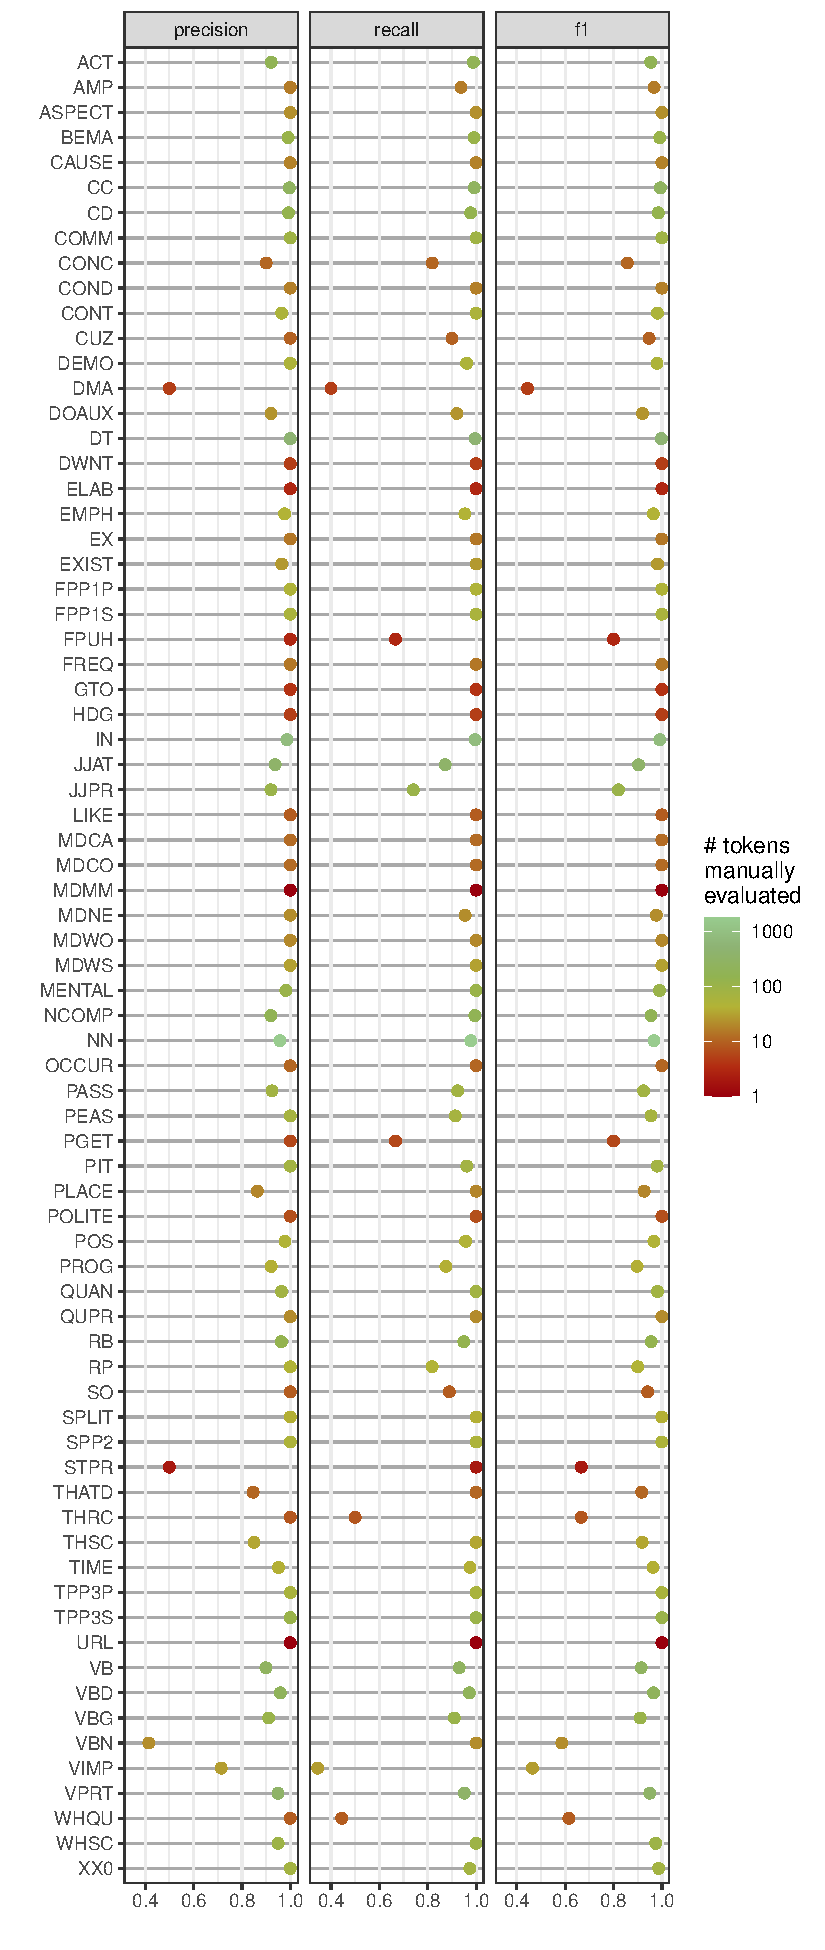
\includegraphics[keepaspectratio]{AppendixD_files/figure-pdf/unnamed-chunk-10-1.pdf}}

\begin{Shaded}
\begin{Highlighting}[]
\CommentTok{\#ggsave(here("plots", "TaggerAccuracyPlot.svg"), width = 7, height = 12)}
\end{Highlighting}
\end{Shaded}

\section{Exploring tagger errors}\label{exploring-tagger-errors}

To inspect regular/systematic tagger errors, we add an error tag with
the incorrectly assigned tag and underscore and then the correct
``gold'' label.

\begin{Shaded}
\begin{Highlighting}[]
\NormalTok{errors }\OtherTok{\textless{}{-}}\NormalTok{ TaggerEval }\SpecialCharTok{|\textgreater{}} 
  \FunctionTok{filter}\NormalTok{(Evaluation}\SpecialCharTok{==}\StringTok{"FALSE"}\NormalTok{) }\SpecialCharTok{|\textgreater{}} 
  \FunctionTok{filter}\NormalTok{(TagGold }\SpecialCharTok{!=} \StringTok{"UNCLEAR"}\NormalTok{) }\SpecialCharTok{|\textgreater{}} 
  \FunctionTok{mutate}\NormalTok{(}\AttributeTok{Error =} \FunctionTok{paste}\NormalTok{(Tag, TagGold, }\AttributeTok{sep =} \StringTok{" {-}\textgreater{} "}\NormalTok{))}

\NormalTok{FreqErrors }\OtherTok{\textless{}{-}}\NormalTok{ errors }\SpecialCharTok{|\textgreater{}} 
  \CommentTok{\#filter(Corpus \%in\% c("TEC{-}Fr", "TEC{-}Ger", "TEC{-}Sp")) |\textgreater{} }
  \FunctionTok{count}\NormalTok{(Error) }\SpecialCharTok{|\textgreater{}} 
  \FunctionTok{arrange}\NormalTok{(}\FunctionTok{desc}\NormalTok{(n))}

\CommentTok{\# Number of error types that only occur once}
\NormalTok{once }\OtherTok{\textless{}{-}}\NormalTok{ FreqErrors }\SpecialCharTok{|\textgreater{}} 
  \FunctionTok{filter}\NormalTok{(n }\SpecialCharTok{==} \DecValTok{1}\NormalTok{) }\SpecialCharTok{|\textgreater{}} 
  \FunctionTok{nrow}\NormalTok{()}
\end{Highlighting}
\end{Shaded}

The total number of errors is 817. Of those, 94 occur just once. In
total, there are 198 different types of errors. The most frequent 10
are:

\begin{Shaded}
\begin{Highlighting}[]
\NormalTok{FreqErrors }\SpecialCharTok{|\textgreater{}} 
  \FunctionTok{filter}\NormalTok{(n }\SpecialCharTok{\textgreater{}} \DecValTok{10}\NormalTok{) }\SpecialCharTok{|\textgreater{}} 
  \FunctionTok{kable}\NormalTok{(}\AttributeTok{digits =} \DecValTok{2}\NormalTok{)}
\end{Highlighting}
\end{Shaded}

\begin{longtable}[]{@{}lr@{}}
\toprule\noalign{}
Error & n \\
\midrule\noalign{}
\endhead
\bottomrule\noalign{}
\endlastfoot
NCOMP -\textgreater{} NULL & 37 \\
NN -\textgreater{} JJAT & 35 \\
JJAT -\textgreater{} NN & 27 \\
NN -\textgreater{} VB & 27 \\
IN -\textgreater{} RP & 25 \\
NN -\textgreater{} VPRT & 24 \\
VB -\textgreater{} NN & 22 \\
THSC -\textgreater{} DEMO & 19 \\
VB -\textgreater{} VIMP & 19 \\
NN -\textgreater{} OCR & 16 \\
VBN -\textgreater{} JJAT & 16 \\
ACT -\textgreater{} NULL & 15 \\
THATD -\textgreater{} NULL & 15 \\
CD -\textgreater{} NN & 12 \\
MENTAL -\textgreater{} NULL & 12 \\
NN -\textgreater{} VBG & 11 \\
NN -\textgreater{} VIMP & 11 \\
THSC -\textgreater{} THRC & 11 \\
VBG -\textgreater{} PROG & 11 \\
VBN -\textgreater{} JJPR & 11 \\
\end{longtable}

The code in the following chunk can be used to take a closer look at
specific types of frequent errors.

\begin{Shaded}
\begin{Highlighting}[]
\NormalTok{errors }\SpecialCharTok{|\textgreater{}} 
  \FunctionTok{filter}\NormalTok{(Error }\SpecialCharTok{==} \StringTok{"NN {-}\textgreater{} JJAT"}\NormalTok{) }\SpecialCharTok{|\textgreater{}} 
  \FunctionTok{select}\NormalTok{(}\SpecialCharTok{{-}}\NormalTok{Output, }\SpecialCharTok{{-}}\NormalTok{Corpus, }\SpecialCharTok{{-}}\NormalTok{Tag, }\SpecialCharTok{{-}}\NormalTok{TagGold) }\SpecialCharTok{|\textgreater{}} 
  \FunctionTok{filter}\NormalTok{(}\FunctionTok{grepl}\NormalTok{(}\AttributeTok{x =}\NormalTok{ Token, }\AttributeTok{pattern =} \StringTok{"[A{-}Z]+."}\NormalTok{)) }\SpecialCharTok{|\textgreater{}} 
  \FunctionTok{kable}\NormalTok{(}\AttributeTok{digits =} \DecValTok{2}\NormalTok{)}
\end{Highlighting}
\end{Shaded}

\begin{longtable}[]{@{}lllll@{}}
\toprule\noalign{}
FileID & Register & Token & Evaluation & Error \\
\midrule\noalign{}
\endhead
\bottomrule\noalign{}
\endlastfoot
BNCBEFor32 & internet & Intermediate & FALSE & NN -\textgreater{}
JJAT \\
BNCBMass16 & news & FINAL & FALSE & NN -\textgreater{} JJAT \\
BNCBMass16 & news & Big & FALSE & NN -\textgreater{} JJAT \\
BNCBReg111 & news & Scottish & FALSE & NN -\textgreater{} JJAT \\
BNCBReg111 & news & Scottish & FALSE & NN -\textgreater{} JJAT \\
BNCBReg111 & news & Mental & FALSE & NN -\textgreater{} JJAT \\
BNCBReg111 & news & Scottish & FALSE & NN -\textgreater{} JJAT \\
BNCBReg111 & news & Central & FALSE & NN -\textgreater{} JJAT \\
BNCBReg750 & news & English & FALSE & NN -\textgreater{} JJAT \\
BNCBReg750 & news & Natural & FALSE & NN -\textgreater{} JJAT \\
BNCBReg750 & news & European & FALSE & NN -\textgreater{} JJAT \\
BNCBReg750 & news & Christian & FALSE & NN -\textgreater{} JJAT \\
BNCBReg750 & news & Social & FALSE & NN -\textgreater{} JJAT \\
BNCBReg750 & news & Common & FALSE & NN -\textgreater{} JJAT \\
BNCBSer486 & news & Northern & FALSE & NN -\textgreater{} JJAT \\
BNCBSer486 & news & Northern & FALSE & NN -\textgreater{} JJAT \\
BNCBSer486 & news & Northern & FALSE & NN -\textgreater{} JJAT \\
BNCBSer562 & news & United & FALSE & NN -\textgreater{} JJAT \\
BNCBSer562 & news & White & FALSE & NN -\textgreater{} JJAT \\
BNCBSer562 & news & Untold & FALSE & NN -\textgreater{} JJAT \\
BNCBSer562 & news & New & FALSE & NN -\textgreater{} JJAT \\
SEL5 & spoken & Black & FALSE & NN -\textgreater{} JJAT \\
\end{longtable}

\begin{Shaded}
\begin{Highlighting}[]
\NormalTok{errors }\SpecialCharTok{|\textgreater{}} 
  \FunctionTok{filter}\NormalTok{(Error }\SpecialCharTok{\%in\%} \FunctionTok{c}\NormalTok{(}\StringTok{"NN {-}\textgreater{} VB"}\NormalTok{, }\StringTok{"VB {-}\textgreater{} NN"}\NormalTok{, }\StringTok{"NN {-}\textgreater{} VPRT"}\NormalTok{, }\StringTok{"VPRT {-}\textgreater{} NN"}\NormalTok{)) }\SpecialCharTok{|\textgreater{}} 
  \FunctionTok{count}\NormalTok{(Token) }\SpecialCharTok{|\textgreater{}} 
  \FunctionTok{arrange}\NormalTok{(}\FunctionTok{desc}\NormalTok{(n)) }\SpecialCharTok{|\textgreater{}} 
  \FunctionTok{filter}\NormalTok{(n }\SpecialCharTok{\textgreater{}} \DecValTok{1}\NormalTok{) }\SpecialCharTok{|\textgreater{}} 
  \FunctionTok{kable}\NormalTok{(}\AttributeTok{digits =} \DecValTok{2}\NormalTok{) }
\end{Highlighting}
\end{Shaded}

\begin{longtable}[]{@{}lr@{}}
\toprule\noalign{}
Token & n \\
\midrule\noalign{}
\endhead
\bottomrule\noalign{}
\endlastfoot
mince & 5 \\
build & 4 \\
win & 4 \\
hunt & 3 \\
wags & 3 \\
throw & 2 \\
look & 2 \\
swamp & 2 \\
stop & 2 \\
defeats & 2 \\
\end{longtable}

\begin{Shaded}
\begin{Highlighting}[]
\NormalTok{errors }\SpecialCharTok{|\textgreater{}} 
  \FunctionTok{filter}\NormalTok{(Error }\SpecialCharTok{==} \StringTok{"ACT {-}\textgreater{} NULL"}\NormalTok{) }\SpecialCharTok{|\textgreater{}} 
  \FunctionTok{count}\NormalTok{(Token) }\SpecialCharTok{|\textgreater{}} 
  \FunctionTok{arrange}\NormalTok{(}\FunctionTok{desc}\NormalTok{(n)) }\SpecialCharTok{|\textgreater{}} 
  \FunctionTok{kable}\NormalTok{(}\AttributeTok{digits =} \DecValTok{2}\NormalTok{) }
\end{Highlighting}
\end{Shaded}

\begin{longtable}[]{@{}lr@{}}
\toprule\noalign{}
Token & n \\
\midrule\noalign{}
\endhead
\bottomrule\noalign{}
\endlastfoot
win & 3 \\
throw & 2 \\
lost & 2 \\
left & 1 \\
waiting & 1 \\
working & 1 \\
running & 1 \\
done & 1 \\
fixed & 1 \\
Play & 1 \\
reached & 1 \\
\end{longtable}

For more information on the MFTE evaluation, see (Le Foll 2021b) and
\url{https://github.com/elenlefoll/MultiFeatureTaggerEnglish}.

\section{Packages used in this
script}\label{packages-used-in-this-script}

\subsection{Package names and
versions}\label{package-names-and-versions}

\begin{verbatim}
R version 4.4.1 (2024-06-14)
Platform: aarch64-apple-darwin20
Running under: macOS Sonoma 14.5

Matrix products: default
BLAS:   /Library/Frameworks/R.framework/Versions/4.4-arm64/Resources/lib/libRblas.0.dylib 
LAPACK: /Library/Frameworks/R.framework/Versions/4.4-arm64/Resources/lib/libRlapack.dylib;  LAPACK version 3.12.0

locale:
[1] en_US.UTF-8/en_US.UTF-8/en_US.UTF-8/C/en_US.UTF-8/en_US.UTF-8

time zone: Europe/Madrid
tzcode source: internal

attached base packages:
[1] stats     graphics  grDevices datasets  utils     methods   base     

other attached packages:
 [1] lubridate_1.9.3   forcats_1.0.0     stringr_1.5.1     dplyr_1.1.4      
 [5] purrr_1.0.2       readr_2.1.5       tidyr_1.3.1       tibble_3.2.1     
 [9] tidyverse_2.0.0   readxl_1.4.3      paletteer_1.6.0   knitr_1.48       
[13] here_1.0.1        harrypotter_2.1.1 caret_6.0-94      lattice_0.22-6   
[17] ggplot2_3.5.1    

loaded via a namespace (and not attached):
 [1] tidyselect_1.2.1     timeDate_4032.109    fastmap_1.2.0       
 [4] pROC_1.18.5          digest_0.6.36        rpart_4.1.23        
 [7] timechange_0.3.0     lifecycle_1.0.4      survival_3.6-4      
[10] magrittr_2.0.3       compiler_4.4.1       rlang_1.1.4         
[13] tools_4.4.1          utf8_1.2.4           yaml_2.3.9          
[16] data.table_1.15.4    plyr_1.8.9           withr_3.0.0         
[19] nnet_7.3-19          grid_4.4.1           stats4_4.4.1        
[22] fansi_1.0.6          colorspace_2.1-0     future_1.33.2       
[25] globals_0.16.3       scales_1.3.0         iterators_1.0.14    
[28] MASS_7.3-60.2        cli_3.6.3            rmarkdown_2.27      
[31] generics_0.1.3       rstudioapi_0.16.0    future.apply_1.11.2 
[34] tzdb_0.4.0           reshape2_1.4.4       splines_4.4.1       
[37] parallel_4.4.1       BiocManager_1.30.23  cellranger_1.1.0    
[40] vctrs_0.6.5          hardhat_1.4.0        Matrix_1.7-0        
[43] jsonlite_1.8.8       hms_1.1.3            listenv_0.9.1       
[46] foreach_1.5.2        gower_1.0.1          recipes_1.1.0       
[49] glue_1.7.0           parallelly_1.37.1    rematch2_2.1.2      
[52] codetools_0.2-20     stringi_1.8.4        gtable_0.3.5        
[55] munsell_0.5.1        pillar_1.9.0         htmltools_0.5.8.1   
[58] ipred_0.9-15         lava_1.8.0           R6_2.5.1            
[61] rprojroot_2.0.4      evaluate_0.24.0      renv_1.0.3          
[64] class_7.3-22         Rcpp_1.0.13          gridExtra_2.3       
[67] nlme_3.1-164         prodlim_2024.06.25   xfun_0.46           
[70] ModelMetrics_1.2.2.2 pkgconfig_2.0.3     
\end{verbatim}

\subsection{Package references}\label{package-references}

{[}1{]} S. A. file. \emph{paletteer: Comprehensive Collection of Color
Palettes}. R package version 1.6.0. 2024.
\url{https://github.com/EmilHvitfeldt/paletteer}.

{[}2{]} G. Grolemund and H. Wickham. ``Dates and Times Made Easy with
lubridate''. In: \emph{Journal of Statistical Software} 40.3 (2011), pp.
1-25. \url{https://www.jstatsoft.org/v40/i03/}.

{[}3{]} A. Jimenez Rico. \emph{harrypotter: Palettes Generated from All
``Harry Potter'' Movies}. R package version 2.1.1. 2020.
\url{https://github.com/aljrico/harrypotter}.

{[}4{]} M. Kuhn. \emph{caret: Classification and Regression Training}. R
package version 6.0-94. 2023. \url{https://github.com/topepo/caret/}.

{[}5{]} Kuhn and Max. ``Building Predictive Models in R Using the caret
Package''. In: \emph{Journal of Statistical Software} 28.5 (2008),
p.~1--26. DOI: 10.18637/jss.v028.i05.
\url{https://www.jstatsoft.org/index.php/jss/article/view/v028i05}.

{[}6{]} K. Müller. \emph{here: A Simpler Way to Find Your Files}. R
package version 1.0.1. 2020. \url{https://here.r-lib.org/}.

{[}7{]} K. Müller and H. Wickham. \emph{tibble: Simple Data Frames}. R
package version 3.2.1. 2023. \url{https://tibble.tidyverse.org/}.

{[}8{]} R Core Team. \emph{R: A Language and Environment for Statistical
Computing}. R Foundation for Statistical Computing. Vienna, Austria,
2024. \url{https://www.R-project.org/}.

{[}9{]} D. Sarkar. \emph{Lattice: Multivariate Data Visualization with
R}. New York: Springer, 2008. ISBN: 978-0-387-75968-5.
\url{http://lmdvr.r-forge.r-project.org}.

{[}10{]} D. Sarkar. \emph{lattice: Trellis Graphics for R}. R package
version 0.22-6. 2024. \url{https://lattice.r-forge.r-project.org/}.

{[}11{]} V. Spinu, G. Grolemund, and H. Wickham. \emph{lubridate: Make
Dealing with Dates a Little Easier}. R package version 1.9.3. 2023.
\url{https://lubridate.tidyverse.org}.

{[}12{]} H. Wickham. \emph{forcats: Tools for Working with Categorical
Variables (Factors)}. R package version 1.0.0. 2023.
\url{https://forcats.tidyverse.org/}.

{[}13{]} H. Wickham. \emph{ggplot2: Elegant Graphics for Data Analysis}.
Springer-Verlag New York, 2016. ISBN: 978-3-319-24277-4.
\url{https://ggplot2.tidyverse.org}.

{[}14{]} H. Wickham. \emph{stringr: Simple, Consistent Wrappers for
Common String Operations}. R package version 1.5.1. 2023.
\url{https://stringr.tidyverse.org}.

{[}15{]} H. Wickham. \emph{tidyverse: Easily Install and Load the
Tidyverse}. R package version 2.0.0. 2023.
\url{https://tidyverse.tidyverse.org}.

{[}16{]} H. Wickham, M. Averick, J. Bryan, et al.~``Welcome to the
tidyverse''. In: \emph{Journal of Open Source Software} 4.43 (2019),
p.~1686. DOI: 10.21105/joss.01686.

{[}17{]} H. Wickham and J. Bryan. \emph{readxl: Read Excel Files}. R
package version 1.4.3. 2023. \url{https://readxl.tidyverse.org}.

{[}18{]} H. Wickham, W. Chang, L. Henry, et al.~\emph{ggplot2: Create
Elegant Data Visualisations Using the Grammar of Graphics}. R package
version 3.5.1. 2024. \url{https://ggplot2.tidyverse.org}.

{[}19{]} H. Wickham, R. François, L. Henry, et al.~\emph{dplyr: A
Grammar of Data Manipulation}. R package version 1.1.4. 2023.
\url{https://dplyr.tidyverse.org}.

{[}20{]} H. Wickham and L. Henry. \emph{purrr: Functional Programming
Tools}. R package version 1.0.2. 2023.
\url{https://purrr.tidyverse.org/}.

{[}21{]} H. Wickham, J. Hester, and J. Bryan. \emph{readr: Read
Rectangular Text Data}. R package version 2.1.5. 2024.
\url{https://readr.tidyverse.org}.

{[}22{]} H. Wickham, D. Vaughan, and M. Girlich. \emph{tidyr: Tidy Messy
Data}. R package version 1.3.1. 2024. \url{https://tidyr.tidyverse.org}.

{[}23{]} Y. Xie. \emph{Dynamic Documents with R and knitr}. 2nd. ISBN
978-1498716963. Boca Raton, Florida: Chapman and Hall/CRC, 2015.
\url{https://yihui.org/knitr/}.

{[}24{]} Y. Xie. ``knitr: A Comprehensive Tool for Reproducible Research
in R''. In: \emph{Implementing Reproducible Computational Research}. Ed.
by V. Stodden, F. Leisch and R. D. Peng. ISBN 978-1466561595. Chapman
and Hall/CRC, 2014.

{[}25{]} Y. Xie. \emph{knitr: A General-Purpose Package for Dynamic
Report Generation in R}. R package version 1.48. 2024.
\url{https://yihui.org/knitr/}.

\chapter{Data Preparation for the Model of Intra-Textbook
Variation}\label{data-preparation-for-the-model-of-intra-textbook-variation}

This script documents the steps taken to pre-process the Textbook
English Corpus (TEC) data that were entered in the multi-dimensional
model of intra-textbook linguistic variation (Chapter 6).

\section{Packages required}\label{packages-required}

The following packages must be installed and loaded to process the data.

\begin{Shaded}
\begin{Highlighting}[]
\CommentTok{\#renv::restore() \# Restore the project\textquotesingle{}s dependencies from the lockfile to ensure that same package versions are used as in the original study}

\FunctionTok{library}\NormalTok{(caret) }\CommentTok{\# For its confusion matrix function}
\FunctionTok{library}\NormalTok{(DT) }\CommentTok{\# To display interactive HTML tables}
\FunctionTok{library}\NormalTok{(here) }\CommentTok{\# For dynamic file paths}
\FunctionTok{library}\NormalTok{(knitr) }\CommentTok{\# Loaded to display the tables using the kable() function}
\FunctionTok{library}\NormalTok{(patchwork) }\CommentTok{\# Needed to put together Fig. 1}
\FunctionTok{library}\NormalTok{(PerformanceAnalytics) }\CommentTok{\# For the correlation plot}
\FunctionTok{library}\NormalTok{(psych) }\CommentTok{\# For various useful, stats function}
\FunctionTok{library}\NormalTok{(tidyverse) }\CommentTok{\# For data wrangling}
\end{Highlighting}
\end{Shaded}

\section{Data import from MFTE
output}\label{data-import-from-mfte-output}

The raw data used in this script is a tab-separated file that
corresponds to the tabular output of mixed normalised frequencies as
generated by the
\href{https://github.com/mshakirDr/MultiFeatureTaggerEnglish}{MFTE Perl
v. 3.1} (Le Foll 2021b).

\begin{Shaded}
\begin{Highlighting}[]
\CommentTok{\# Read in Textbook Corpus data}
\NormalTok{TxBcounts }\OtherTok{\textless{}{-}} \FunctionTok{read.delim}\NormalTok{(}\FunctionTok{here}\NormalTok{(}\StringTok{"data"}\NormalTok{, }\StringTok{"MFTE"}\NormalTok{, }\StringTok{"TxB900MDA\_3.1\_normed\_complex\_counts.tsv"}\NormalTok{), }\AttributeTok{header =} \ConstantTok{TRUE}\NormalTok{, }\AttributeTok{stringsAsFactors =} \ConstantTok{TRUE}\NormalTok{)}

\NormalTok{TxBcounts }\OtherTok{\textless{}{-}}\NormalTok{ TxBcounts }\SpecialCharTok{|\textgreater{}} 
  \FunctionTok{filter}\NormalTok{(Filename}\SpecialCharTok{!=}\StringTok{".DS\_Store"}\NormalTok{) }\SpecialCharTok{|\textgreater{}}  
  \FunctionTok{droplevels}\NormalTok{()}

\CommentTok{\#str(TxBcounts) \# Check sanity of data}
\CommentTok{\#nrow(TxBcounts) \# Should be 2014 files}

\FunctionTok{datatable}\NormalTok{(TxBcounts,}
  \AttributeTok{filter =} \StringTok{"top"}\NormalTok{,}
\NormalTok{) }\SpecialCharTok{|\textgreater{}} 
  \FunctionTok{formatRound}\NormalTok{(}\DecValTok{3}\SpecialCharTok{:}\FunctionTok{ncol}\NormalTok{(TxBcounts), }\AttributeTok{digits=}\DecValTok{2}\NormalTok{)}
\end{Highlighting}
\end{Shaded}

\pandocbounded{
\includegraphics[keepaspectratio]{AppendixE_files/figure-pdf/raw_data-1.pdf}}

Metadata was added on the basis of the filenames.

\begin{Shaded}
\begin{Highlighting}[]
\CommentTok{\# Adding a textbook proficiency level}
\NormalTok{TxBLevels }\OtherTok{\textless{}{-}} \FunctionTok{read.delim}\NormalTok{(}\FunctionTok{here}\NormalTok{(}\StringTok{"data"}\NormalTok{, }\StringTok{"metadata"}\NormalTok{, }\StringTok{"TxB900MDA\_ProficiencyLevels.csv"}\NormalTok{), }\AttributeTok{sep =} \StringTok{","}\NormalTok{)}
\NormalTok{TxBcounts }\OtherTok{\textless{}{-}} \FunctionTok{full\_join}\NormalTok{(TxBcounts, TxBLevels, }\AttributeTok{by =} \StringTok{"Filename"}\NormalTok{) }\SpecialCharTok{|\textgreater{}}  
  \FunctionTok{mutate}\NormalTok{(}\AttributeTok{Level =} \FunctionTok{as.factor}\NormalTok{(Level)) }\SpecialCharTok{|\textgreater{}}  
  \FunctionTok{mutate}\NormalTok{(}\AttributeTok{Filename =} \FunctionTok{as.factor}\NormalTok{(Filename))}

\CommentTok{\# Check distribution and that there are no NAs}
\FunctionTok{summary}\NormalTok{(TxBcounts}\SpecialCharTok{$}\NormalTok{Level) }\SpecialCharTok{|\textgreater{}} 
  \FunctionTok{kable}\NormalTok{(}\AttributeTok{col.names =} \FunctionTok{c}\NormalTok{(}\StringTok{"Textbook Level"}\NormalTok{, }\StringTok{"\# of texts"}\NormalTok{))}
\end{Highlighting}
\end{Shaded}

\begin{longtable}[]{@{}lr@{}}
\toprule\noalign{}
Textbook Level & \# of texts \\
\midrule\noalign{}
\endhead
\bottomrule\noalign{}
\endlastfoot
A & 292 \\
B & 407 \\
C & 506 \\
D & 478 \\
E & 331 \\
\end{longtable}

\begin{Shaded}
\begin{Highlighting}[]
\CommentTok{\# Check matching on random sample}
\CommentTok{\# TxBcounts |\textgreater{}}
\CommentTok{\#   select(Filename, Level) |\textgreater{}  }
\CommentTok{\#   sample\_n(20) }

\CommentTok{\# Adding a register variable from the file names}
\NormalTok{TxBcounts}\SpecialCharTok{$}\NormalTok{Register }\OtherTok{\textless{}{-}} \FunctionTok{as.factor}\NormalTok{(stringr}\SpecialCharTok{::}\FunctionTok{str\_extract}\NormalTok{(TxBcounts}\SpecialCharTok{$}\NormalTok{Filename, }\StringTok{"Spoken|Narrative|Other|Personal|Informative|Instructional|Poetry"}\NormalTok{)) }\CommentTok{\# Add a variable for Textbook Register}
\FunctionTok{summary}\NormalTok{(TxBcounts}\SpecialCharTok{$}\NormalTok{Register) }\SpecialCharTok{|\textgreater{}} 
  \FunctionTok{kable}\NormalTok{(}\AttributeTok{col.names =} \FunctionTok{c}\NormalTok{(}\StringTok{"Textbook Register"}\NormalTok{, }\StringTok{"\# of texts"}\NormalTok{))}
\end{Highlighting}
\end{Shaded}

\begin{longtable}[]{@{}lr@{}}
\toprule\noalign{}
Textbook Register & \# of texts \\
\midrule\noalign{}
\endhead
\bottomrule\noalign{}
\endlastfoot
Informative & 364 \\
Instructional & 647 \\
Narrative & 285 \\
Personal & 88 \\
Poetry & 37 \\
Spoken & 593 \\
\end{longtable}

\begin{Shaded}
\begin{Highlighting}[]
\NormalTok{TxBcounts}\SpecialCharTok{$}\NormalTok{Register }\OtherTok{\textless{}{-}}\NormalTok{ car}\SpecialCharTok{::}\FunctionTok{recode}\NormalTok{(TxBcounts}\SpecialCharTok{$}\NormalTok{Register, }\StringTok{"\textquotesingle{}Narrative\textquotesingle{} = \textquotesingle{}Fiction\textquotesingle{}; \textquotesingle{}Spoken\textquotesingle{} = \textquotesingle{}Conversation\textquotesingle{}"}\NormalTok{)}
\CommentTok{\#colnames(TxBcounts) \# Check all the variables make sense}

\CommentTok{\# Adding a textbook series variable from the file names}
\NormalTok{TxBcounts}\SpecialCharTok{$}\NormalTok{Filename }\OtherTok{\textless{}{-}}\NormalTok{ stringr}\SpecialCharTok{::}\FunctionTok{str\_replace}\NormalTok{(TxBcounts}\SpecialCharTok{$}\NormalTok{Filename, }\StringTok{"English\_In\_Mind|English\_in\_Mind"}\NormalTok{, }\StringTok{"EIM"}\NormalTok{) }
\NormalTok{TxBcounts}\SpecialCharTok{$}\NormalTok{Filename }\OtherTok{\textless{}{-}}\NormalTok{ stringr}\SpecialCharTok{::}\FunctionTok{str\_replace}\NormalTok{(TxBcounts}\SpecialCharTok{$}\NormalTok{Filename, }\StringTok{"New\_GreenLine"}\NormalTok{, }\StringTok{"NGL"}\NormalTok{) }\CommentTok{\# Otherwise the regex for GreenLine will override New\_GreenLine}
\NormalTok{TxBcounts}\SpecialCharTok{$}\NormalTok{Filename }\OtherTok{\textless{}{-}}\NormalTok{ stringr}\SpecialCharTok{::}\FunctionTok{str\_replace}\NormalTok{(TxBcounts}\SpecialCharTok{$}\NormalTok{Filename, }\StringTok{"Piece\_of\_cake"}\NormalTok{, }\StringTok{"POC"}\NormalTok{) }\CommentTok{\# Shorten label for ease of plotting}
\NormalTok{TxBcounts}\SpecialCharTok{$}\NormalTok{Series }\OtherTok{\textless{}{-}} \FunctionTok{as.factor}\NormalTok{(stringr}\SpecialCharTok{::}\FunctionTok{str\_extract}\NormalTok{(TxBcounts}\SpecialCharTok{$}\NormalTok{Filename, }\StringTok{"Access|Achievers|EIM|GreenLine|HT|NB|NM|POC|JTT|NGL|Solutions"}\NormalTok{)) }\CommentTok{\# Extract textbook series from (ammended) filenames}
\FunctionTok{summary}\NormalTok{(TxBcounts}\SpecialCharTok{$}\NormalTok{Series)  }\SpecialCharTok{|\textgreater{}} 
  \FunctionTok{kable}\NormalTok{(}\AttributeTok{col.names =} \FunctionTok{c}\NormalTok{(}\StringTok{"Textbook Name"}\NormalTok{, }\StringTok{"\# of texts"}\NormalTok{))}
\end{Highlighting}
\end{Shaded}

\begin{longtable}[]{@{}lr@{}}
\toprule\noalign{}
Textbook Name & \# of texts \\
\midrule\noalign{}
\endhead
\bottomrule\noalign{}
\endlastfoot
Access & 315 \\
Achievers & 240 \\
EIM & 180 \\
GreenLine & 209 \\
HT & 115 \\
JTT & 129 \\
NB & 44 \\
NGL & 298 \\
NM & 59 \\
POC & 98 \\
Solutions & 327 \\
\end{longtable}

\begin{Shaded}
\begin{Highlighting}[]
\CommentTok{\# Including the French textbooks for the first year of Lycée to their corresponding publisher series from collège}
\NormalTok{TxBcounts}\SpecialCharTok{$}\NormalTok{Series }\OtherTok{\textless{}{-}}\NormalTok{car}\SpecialCharTok{::}\FunctionTok{recode}\NormalTok{(TxBcounts}\SpecialCharTok{$}\NormalTok{Series, }\StringTok{"c(\textquotesingle{}NB\textquotesingle{}, \textquotesingle{}JTT\textquotesingle{}) = \textquotesingle{}JTT\textquotesingle{}; c(\textquotesingle{}NM\textquotesingle{}, \textquotesingle{}HT\textquotesingle{}) = \textquotesingle{}HT\textquotesingle{}"}\NormalTok{) }\CommentTok{\# Recode final volumes of French series (see Section 4.3.1.1 on textbook selection for details)}
\FunctionTok{summary}\NormalTok{(TxBcounts}\SpecialCharTok{$}\NormalTok{Series) }\SpecialCharTok{|\textgreater{}} 
  \FunctionTok{kable}\NormalTok{(}\AttributeTok{col.names =} \FunctionTok{c}\NormalTok{(}\StringTok{"Textbook Series"}\NormalTok{, }\StringTok{"\# of texts"}\NormalTok{))}
\end{Highlighting}
\end{Shaded}

\begin{longtable}[]{@{}lr@{}}
\toprule\noalign{}
Textbook Series & \# of texts \\
\midrule\noalign{}
\endhead
\bottomrule\noalign{}
\endlastfoot
Access & 315 \\
Achievers & 240 \\
EIM & 180 \\
GreenLine & 209 \\
HT & 174 \\
JTT & 173 \\
NGL & 298 \\
POC & 98 \\
Solutions & 327 \\
\end{longtable}

\begin{Shaded}
\begin{Highlighting}[]
\CommentTok{\# Adding a textbook country of use variable from the series variable}
\NormalTok{TxBcounts}\SpecialCharTok{$}\NormalTok{Country }\OtherTok{\textless{}{-}}\NormalTok{ TxBcounts}\SpecialCharTok{$}\NormalTok{Series}
\NormalTok{TxBcounts}\SpecialCharTok{$}\NormalTok{Country }\OtherTok{\textless{}{-}}\NormalTok{ car}\SpecialCharTok{::}\FunctionTok{recode}\NormalTok{(TxBcounts}\SpecialCharTok{$}\NormalTok{Series, }\StringTok{"c(\textquotesingle{}Access\textquotesingle{}, \textquotesingle{}GreenLine\textquotesingle{}, \textquotesingle{}NGL\textquotesingle{}) = \textquotesingle{}Germany\textquotesingle{}; c(\textquotesingle{}Achievers\textquotesingle{}, \textquotesingle{}EIM\textquotesingle{}, \textquotesingle{}Solutions\textquotesingle{}) = \textquotesingle{}Spain\textquotesingle{}; c(\textquotesingle{}HT\textquotesingle{}, \textquotesingle{}NB\textquotesingle{}, \textquotesingle{}NM\textquotesingle{}, \textquotesingle{}POC\textquotesingle{}, \textquotesingle{}JTT\textquotesingle{}) = \textquotesingle{}France\textquotesingle{}"}\NormalTok{)}
\FunctionTok{summary}\NormalTok{(TxBcounts}\SpecialCharTok{$}\NormalTok{Country) }\SpecialCharTok{|\textgreater{}} 
  \FunctionTok{kable}\NormalTok{(}\AttributeTok{col.names =} \FunctionTok{c}\NormalTok{(}\StringTok{"Country of Use"}\NormalTok{, }\StringTok{"\# of texts"}\NormalTok{))}
\end{Highlighting}
\end{Shaded}

\begin{longtable}[]{@{}lr@{}}
\toprule\noalign{}
Country of Use & \# of texts \\
\midrule\noalign{}
\endhead
\bottomrule\noalign{}
\endlastfoot
France & 445 \\
Germany & 822 \\
Spain & 747 \\
\end{longtable}

\begin{Shaded}
\begin{Highlighting}[]
\CommentTok{\# Re{-}order variables}
\CommentTok{\#colnames(TxBcounts)}
\NormalTok{TxBcounts }\OtherTok{\textless{}{-}} \FunctionTok{select}\NormalTok{(TxBcounts, }\FunctionTok{order}\NormalTok{(}\FunctionTok{names}\NormalTok{(TxBcounts))) }\SpecialCharTok{\%\textgreater{}\%}
  \FunctionTok{select}\NormalTok{(Filename, Country, Series, Level, Register, Words, }\FunctionTok{everything}\NormalTok{())}
\CommentTok{\#colnames(TxBcounts)}
\end{Highlighting}
\end{Shaded}

\subsection{Corpus size}\label{corpus-size}

This table provides some summary statistics about the number of words
included in the TEC texts originally tagged for this study.

\begin{Shaded}
\begin{Highlighting}[]
\NormalTok{TxBcounts  }\SpecialCharTok{|\textgreater{}}  
  \FunctionTok{group\_by}\NormalTok{(Register) }\SpecialCharTok{|\textgreater{}}  
  \FunctionTok{summarise}\NormalTok{(}\AttributeTok{totaltexts =} \FunctionTok{n}\NormalTok{(), }\AttributeTok{totalwords =} \FunctionTok{sum}\NormalTok{(Words), }\AttributeTok{mean =} \FunctionTok{as.integer}\NormalTok{(}\FunctionTok{mean}\NormalTok{(Words)), }\AttributeTok{sd =} \FunctionTok{as.integer}\NormalTok{(}\FunctionTok{sd}\NormalTok{(Words)), }\AttributeTok{TTRmean =} \FunctionTok{mean}\NormalTok{(TTR)) }\SpecialCharTok{|\textgreater{}}  
  \FunctionTok{kable}\NormalTok{(}\AttributeTok{digits =} \DecValTok{2}\NormalTok{, }\AttributeTok{format.args =} \FunctionTok{list}\NormalTok{(}\AttributeTok{big.mark =} \StringTok{","}\NormalTok{))}
\end{Highlighting}
\end{Shaded}

\begin{longtable}[]{@{}lrrrrr@{}}
\toprule\noalign{}
Register & totaltexts & totalwords & mean & sd & TTRmean \\
\midrule\noalign{}
\endhead
\bottomrule\noalign{}
\endlastfoot
Conversation & 593 & 505,147 & 851 & 301 & 0.44 \\
Fiction & 285 & 241,512 & 847 & 208 & 0.47 \\
Informative & 364 & 304,695 & 837 & 177 & 0.51 \\
Instructional & 647 & 585,049 & 904 & 94 & 0.42 \\
Personal & 88 & 69,570 & 790 & 177 & 0.48 \\
Poetry & 37 & 26,445 & 714 & 192 & 0.44 \\
\end{longtable}

\begin{Shaded}
\begin{Highlighting}[]
\CommentTok{\#TxBcounts \textless{}{-} saveRDS(TxBcounts, here("data", "processed", "TxBcounts.rds"))}
\end{Highlighting}
\end{Shaded}

\section{Data preparation for PCA}\label{data-preparation-for-pca}

Poetry texts were removed for this analysis as there were too few
compared to the other register categories.

\begin{Shaded}
\begin{Highlighting}[]
\FunctionTok{summary}\NormalTok{(TxBcounts}\SpecialCharTok{$}\NormalTok{Register) }\SpecialCharTok{|\textgreater{}}  
  \FunctionTok{kable}\NormalTok{(}\AttributeTok{col.names =} \FunctionTok{c}\NormalTok{(}\StringTok{"Register"}\NormalTok{, }\StringTok{"\# texts"}\NormalTok{))}
\end{Highlighting}
\end{Shaded}

\begin{longtable}[]{@{}lr@{}}
\toprule\noalign{}
Register & \# texts \\
\midrule\noalign{}
\endhead
\bottomrule\noalign{}
\endlastfoot
Conversation & 593 \\
Fiction & 285 \\
Informative & 364 \\
Instructional & 647 \\
Personal & 88 \\
Poetry & 37 \\
\end{longtable}

This led to the following distribution of texts across the five textbook
English registers examined in the model of intra-textbook linguistic
variation:

\begin{Shaded}
\begin{Highlighting}[]
\NormalTok{TxBcounts }\OtherTok{\textless{}{-}}\NormalTok{ TxBcounts }\SpecialCharTok{|\textgreater{}}  
  \FunctionTok{filter}\NormalTok{(Register}\SpecialCharTok{!=}\StringTok{"Poetry"}\NormalTok{) }\SpecialCharTok{|\textgreater{}}  
  \FunctionTok{droplevels}\NormalTok{()}

\FunctionTok{summary}\NormalTok{(TxBcounts}\SpecialCharTok{$}\NormalTok{Register) }\SpecialCharTok{|\textgreater{}}  
  \FunctionTok{kable}\NormalTok{(}\AttributeTok{col.names =} \FunctionTok{c}\NormalTok{(}\StringTok{"Register"}\NormalTok{, }\StringTok{"\# texts"}\NormalTok{))}
\end{Highlighting}
\end{Shaded}

\begin{longtable}[]{@{}lr@{}}
\toprule\noalign{}
Register & \# texts \\
\midrule\noalign{}
\endhead
\bottomrule\noalign{}
\endlastfoot
Conversation & 593 \\
Fiction & 285 \\
Informative & 364 \\
Instructional & 647 \\
Personal & 88 \\
\end{longtable}

\subsection{Feature distributions}\label{feature-distributions}

The distributions of each linguistic features were examined by means of
visualisation. As shown below, before transformation, many of the
features displayed highly skewed distributions.

\begin{Shaded}
\begin{Highlighting}[]
\NormalTok{TxBcounts }\SpecialCharTok{|\textgreater{}} 
  \FunctionTok{select}\NormalTok{(}\SpecialCharTok{{-}}\NormalTok{Words) }\SpecialCharTok{|\textgreater{}}  
  \FunctionTok{keep}\NormalTok{(is.numeric) }\SpecialCharTok{|\textgreater{}}  
\NormalTok{  tidyr}\SpecialCharTok{::}\FunctionTok{gather}\NormalTok{() }\SpecialCharTok{|\textgreater{}}  \CommentTok{\# This function from tidyr converts a selection of variables into two variables: a key and a value. The key contains the names of the original variable and the value the data. This means we can then use the facet\_wrap function from ggplot2}
  \FunctionTok{ggplot}\NormalTok{(}\FunctionTok{aes}\NormalTok{(value)) }\SpecialCharTok{+}
    \FunctionTok{theme\_bw}\NormalTok{() }\SpecialCharTok{+}
    \FunctionTok{facet\_wrap}\NormalTok{(}\SpecialCharTok{\textasciitilde{}}\NormalTok{ key, }\AttributeTok{scales =} \StringTok{"free"}\NormalTok{, }\AttributeTok{ncol =} \DecValTok{4}\NormalTok{) }\SpecialCharTok{+}
    \FunctionTok{scale\_x\_continuous}\NormalTok{(}\AttributeTok{expand=}\FunctionTok{c}\NormalTok{(}\DecValTok{0}\NormalTok{,}\DecValTok{0}\NormalTok{)) }\SpecialCharTok{+}
    \FunctionTok{geom\_histogram}\NormalTok{(}\AttributeTok{bins =} \DecValTok{30}\NormalTok{, }\AttributeTok{colour=} \StringTok{"darkred"}\NormalTok{, }\AttributeTok{fill =} \StringTok{"darkred"}\NormalTok{, }\AttributeTok{alpha =} \FloatTok{0.5}\NormalTok{)}
\end{Highlighting}
\end{Shaded}

\pandocbounded{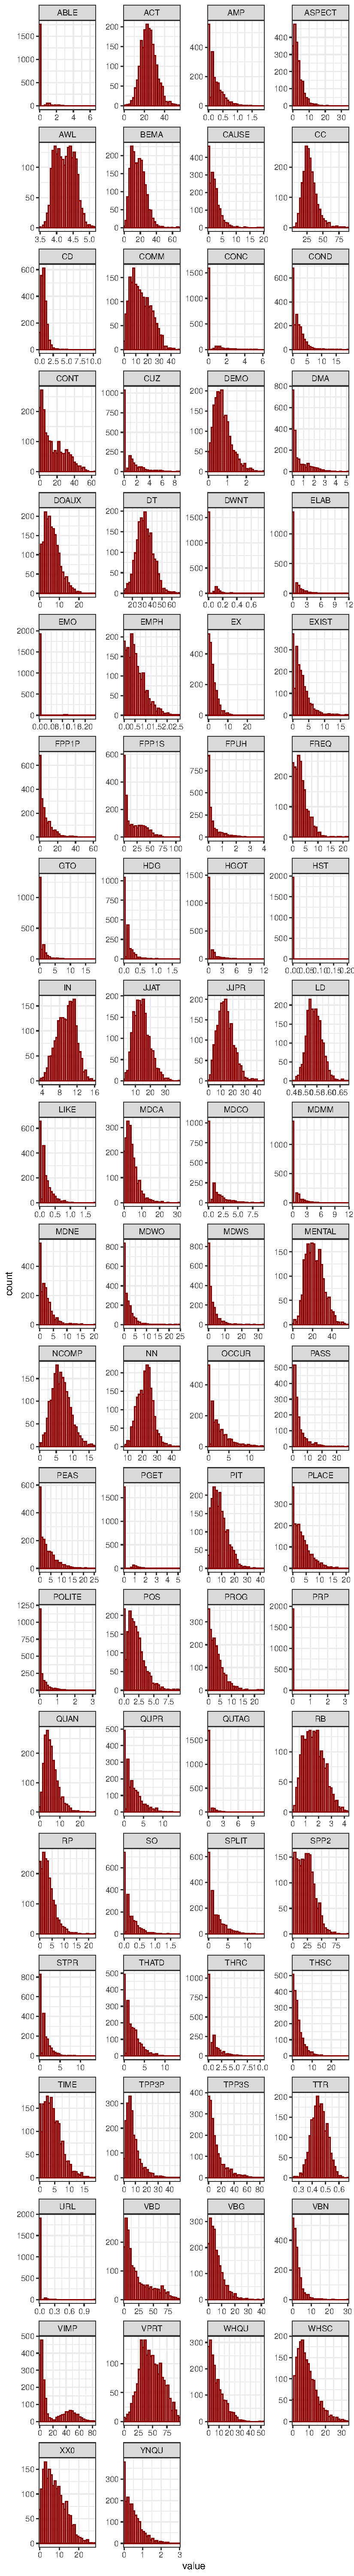
\includegraphics[keepaspectratio]{AppendixE_files/figure-pdf/distribution-viz-1.pdf}}

\begin{Shaded}
\begin{Highlighting}[]
\CommentTok{\#ggsave(here("plots", "TEC{-}HistogramPlotsAllVariablesTEC{-}only.svg"), width = 20, height = 45)}
\end{Highlighting}
\end{Shaded}

\subsection{Feature removal}\label{feature-removal}

A number of features were removed from the dataset as they are not
linguistically interpretable. In the case of the TEC, this included the
variable CD because numbers spelt out as digits were removed from the
textbooks before these were tagged with the MFTE. In addition, the
variables LIKE and SO because these are ``bin'' features included in the
output of the MFTE to ensure that the counts for these polysemous words
do not inflate other categories due to mistags (Le Foll 2021c).

Whenever linguistically meaningful, very low-frequency features were
merged. Finally, features absent from more than third of texts were also
excluded. For the analysis intra-textbook register variation, the
following linguistic features were excluded from the analysis due to low
dispersion:

\begin{Shaded}
\begin{Highlighting}[]
\CommentTok{\# Removal of meaningless features:}
\NormalTok{TxBcounts }\OtherTok{\textless{}{-}}\NormalTok{ TxBcounts }\SpecialCharTok{|\textgreater{}}  
  \FunctionTok{select}\NormalTok{(}\SpecialCharTok{{-}}\FunctionTok{c}\NormalTok{(CD, LIKE, SO))}

\CommentTok{\# Function to compute percentage of texts with occurrences meeting a condition}
\NormalTok{compute\_percentage }\OtherTok{\textless{}{-}} \ControlFlowTok{function}\NormalTok{(data, condition, threshold) \{}
\NormalTok{  numeric\_data }\OtherTok{\textless{}{-}} \FunctionTok{Filter}\NormalTok{(is.numeric, data)}
\NormalTok{  percentage }\OtherTok{\textless{}{-}} \FunctionTok{round}\NormalTok{(}\FunctionTok{colSums}\NormalTok{(condition[, }\FunctionTok{sapply}\NormalTok{(numeric\_data, is.numeric)])}\SpecialCharTok{/}\FunctionTok{nrow}\NormalTok{(data) }\SpecialCharTok{*} \DecValTok{100}\NormalTok{, }\DecValTok{2}\NormalTok{)}
\NormalTok{  percentage }\OtherTok{\textless{}{-}} \FunctionTok{as.data.frame}\NormalTok{(percentage)}
  \FunctionTok{colnames}\NormalTok{(percentage) }\OtherTok{\textless{}{-}} \StringTok{"Percentage"}
\NormalTok{  percentage }\OtherTok{\textless{}{-}}\NormalTok{ percentage }\SpecialCharTok{|\textgreater{}}  
    \FunctionTok{filter}\NormalTok{(}\SpecialCharTok{!}\FunctionTok{is.na}\NormalTok{(Percentage)) }\SpecialCharTok{|\textgreater{}} 
    \FunctionTok{rownames\_to\_column}\NormalTok{() }\SpecialCharTok{|\textgreater{}} 
    \FunctionTok{arrange}\NormalTok{(Percentage)}
  \ControlFlowTok{if}\NormalTok{ (}\SpecialCharTok{!}\FunctionTok{missing}\NormalTok{(threshold)) \{}
\NormalTok{    percentage }\OtherTok{\textless{}{-}}\NormalTok{ percentage }\SpecialCharTok{|\textgreater{}}  
      \FunctionTok{filter}\NormalTok{(Percentage }\SpecialCharTok{\textgreater{}}\NormalTok{ threshold)}
\NormalTok{  \}}
  \FunctionTok{return}\NormalTok{(percentage)}
\NormalTok{\}}

\CommentTok{\# Calculate percentage of texts with 0 occurrences of each feature}
\NormalTok{zero\_features }\OtherTok{\textless{}{-}} \FunctionTok{compute\_percentage}\NormalTok{(TxBcounts, TxBcounts }\SpecialCharTok{==} \DecValTok{0}\NormalTok{, }\FloatTok{66.6}\NormalTok{)}
\CommentTok{\# zero\_features |\textgreater{} }
\CommentTok{\#   kable(col.names = c("Feature", "\% texts with zero occurrences"))}

\CommentTok{\# Combine low frequency features into meaningful groups whenever this makes linguistic sense}
\NormalTok{TxBcounts }\OtherTok{\textless{}{-}}\NormalTok{ TxBcounts }\SpecialCharTok{|\textgreater{}}  
  \FunctionTok{mutate}\NormalTok{(}\AttributeTok{JJPR =}\NormalTok{ ABLE }\SpecialCharTok{+}\NormalTok{ JJPR, }\AttributeTok{ABLE =} \ConstantTok{NULL}\NormalTok{) }\SpecialCharTok{|\textgreater{}}  
  \FunctionTok{mutate}\NormalTok{(}\AttributeTok{PASS =}\NormalTok{ PGET }\SpecialCharTok{+}\NormalTok{ PASS, }\AttributeTok{PGET =} \ConstantTok{NULL}\NormalTok{)}

\CommentTok{\# Re{-}calculate percentage of texts with 0 occurrences of each feature}
\NormalTok{zero\_features2 }\OtherTok{\textless{}{-}} \FunctionTok{compute\_percentage}\NormalTok{(TxBcounts, TxBcounts }\SpecialCharTok{==} \DecValTok{0}\NormalTok{, }\FloatTok{66.6}\NormalTok{)}
\NormalTok{zero\_features2 }\SpecialCharTok{|\textgreater{}} 
  \FunctionTok{kable}\NormalTok{(}\AttributeTok{col.names =} \FunctionTok{c}\NormalTok{(}\StringTok{"Feature"}\NormalTok{, }\StringTok{"\% texts with zero occurrences"}\NormalTok{))}
\end{Highlighting}
\end{Shaded}

\begin{longtable}[]{@{}lr@{}}
\toprule\noalign{}
Feature & \% texts with zero occurrences \\
\midrule\noalign{}
\endhead
\bottomrule\noalign{}
\endlastfoot
GTO & 67.07 \\
ELAB & 69.30 \\
MDMM & 70.81 \\
HGOT & 73.75 \\
CONC & 80.48 \\
DWNT & 81.44 \\
QUTAG & 85.99 \\
URL & 96.51 \\
EMO & 97.82 \\
PRP & 98.33 \\
HST & 99.44 \\
\end{longtable}

\begin{Shaded}
\begin{Highlighting}[]
\CommentTok{\# Drop variables with low document frequency}
\NormalTok{TxBcounts }\OtherTok{\textless{}{-}} \FunctionTok{select}\NormalTok{(TxBcounts, }\SpecialCharTok{{-}}\FunctionTok{one\_of}\NormalTok{(zero\_features2}\SpecialCharTok{$}\NormalTok{rowname))}
\CommentTok{\#ncol(TxBcounts){-}8 \# Number of linguistic features remaining}

\CommentTok{\# List of features}
\CommentTok{\#colnames(TxBcounts)}
\end{Highlighting}
\end{Shaded}

These feature removal operations resulted in a feature set of 64
linguistic variables.

\subsection{Identifying potential outlier
texts}\label{identifying-potential-outlier-texts}

All normalised frequencies were normalised to identify any potential
outlier texts.

\begin{Shaded}
\begin{Highlighting}[]
\NormalTok{TxBzcounts }\OtherTok{\textless{}{-}}\NormalTok{ TxBcounts }\SpecialCharTok{|\textgreater{}} 
  \FunctionTok{select}\NormalTok{(}\SpecialCharTok{{-}}\NormalTok{Words) }\SpecialCharTok{|\textgreater{}}  
  \FunctionTok{keep}\NormalTok{(is.numeric) }\SpecialCharTok{|\textgreater{}}  
  \FunctionTok{scale}\NormalTok{()}

\FunctionTok{boxplot}\NormalTok{(TxBzcounts, }\AttributeTok{las =} \DecValTok{3}\NormalTok{, }\AttributeTok{main =} \StringTok{"z{-}scores"}\NormalTok{) }\CommentTok{\# Slow to open!}
\end{Highlighting}
\end{Shaded}

\pandocbounded{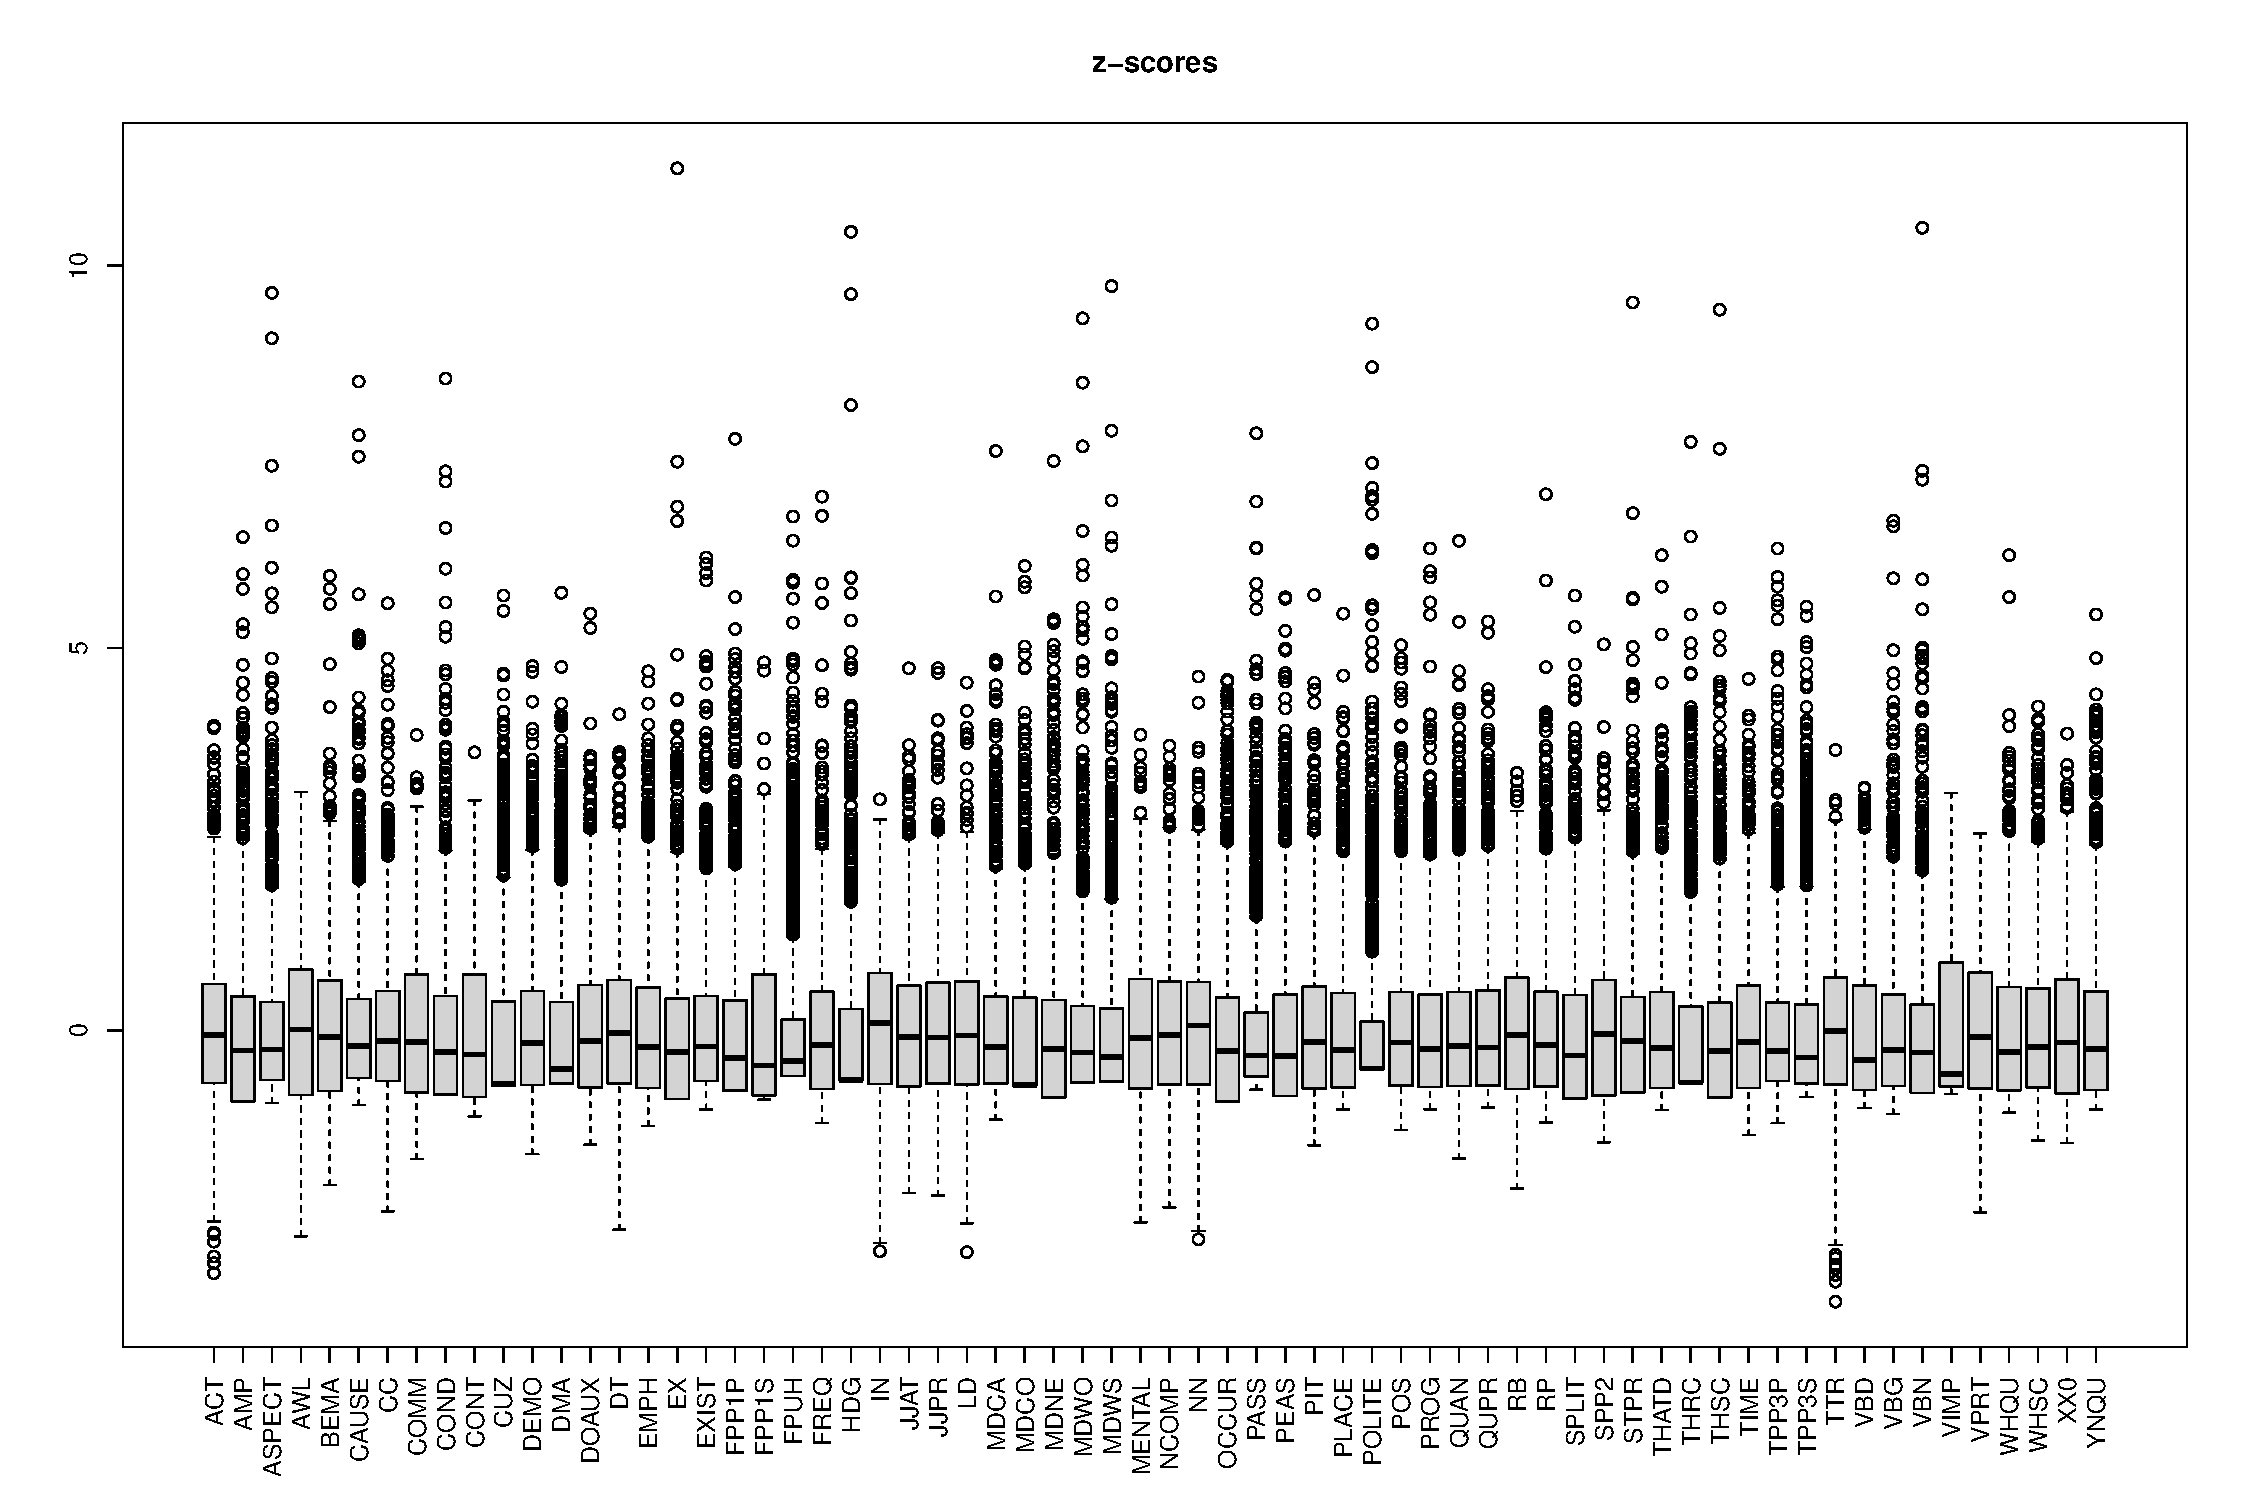
\includegraphics[keepaspectratio]{AppendixE_files/figure-pdf/z-standardisation-outliers-1.pdf}}

\begin{Shaded}
\begin{Highlighting}[]
\CommentTok{\# If necessary, remove any outliers at this stage.}
\NormalTok{TxBdata }\OtherTok{\textless{}{-}} \FunctionTok{cbind}\NormalTok{(TxBcounts[,}\DecValTok{1}\SpecialCharTok{:}\DecValTok{6}\NormalTok{], }\FunctionTok{as.data.frame}\NormalTok{(TxBzcounts))}

\NormalTok{outliers }\OtherTok{\textless{}{-}}\NormalTok{ TxBdata }\SpecialCharTok{|\textgreater{}}  
  \FunctionTok{select}\NormalTok{(}\SpecialCharTok{{-}}\FunctionTok{c}\NormalTok{(Words, LD, TTR)) }\SpecialCharTok{|\textgreater{}}  
  \FunctionTok{filter}\NormalTok{(}\FunctionTok{if\_any}\NormalTok{(}\FunctionTok{where}\NormalTok{(is.numeric), }\SpecialCharTok{\textasciitilde{}}\NormalTok{ .x }\SpecialCharTok{\textgreater{}} \DecValTok{8}\NormalTok{)) }\SpecialCharTok{|\textgreater{}}  
  \FunctionTok{select}\NormalTok{(Filename)}
\end{Highlighting}
\end{Shaded}

The following outlier texts were identified and excluded in subsequent
analyses.

\begin{Shaded}
\begin{Highlighting}[]
\NormalTok{outliers}
\end{Highlighting}
\end{Shaded}

\begin{verbatim}
                                            Filename
1                             POC_4e_Spoken_0007.txt
2             Solutions_Elementary_Personal_0001.txt
3                       NGL_5_Instructional_0018.txt
4                           Access_1_Spoken_0011.txt
5                              EIM_1_Spoken_0012.txt
6                              NGL_4_Spoken_0011.txt
7      Solutions_Intermediate_Plus_Personal_0001.txt
8           Solutions_Elementary_ELF_Spoken_0021.txt
9                          NB_2_Informative_0009.txt
10       Solutions_Intermediate_Plus_Spoken_0022.txt
11     Solutions_Intermediate_Instructional_0025.txt
12 Solutions_Pre-Intermediate_Instructional_0024.txt
13                            POC_4e_Spoken_0010.txt
14            Solutions_Intermediate_Spoken_0019.txt
15                          Access_1_Spoken_0019.txt
16    Solutions_Pre-Intermediate_ELF_Spoken_0005.txt
\end{verbatim}

\begin{Shaded}
\begin{Highlighting}[]
\NormalTok{TxBcounts }\OtherTok{\textless{}{-}}\NormalTok{ TxBcounts }\SpecialCharTok{|\textgreater{}}  
  \FunctionTok{filter}\NormalTok{(}\SpecialCharTok{!}\NormalTok{Filename }\SpecialCharTok{\%in\%}\NormalTok{ outliers}\SpecialCharTok{$}\NormalTok{Filename)}

\CommentTok{\#saveRDS(TxBcounts, here("data", "processed", "TxBcounts3.rds")) \# Last saved 6 March 2024}

\NormalTok{TxBzcounts }\OtherTok{\textless{}{-}}\NormalTok{ TxBcounts }\SpecialCharTok{|\textgreater{}} 
  \FunctionTok{select}\NormalTok{(}\SpecialCharTok{{-}}\NormalTok{Words) }\SpecialCharTok{|\textgreater{}}  
  \FunctionTok{keep}\NormalTok{(is.numeric) }\SpecialCharTok{|\textgreater{}}  
  \FunctionTok{scale}\NormalTok{()}
\end{Highlighting}
\end{Shaded}

This resulted in 1,961 TEC texts being included in the model of
intra-textbook linguistic variation with the following standardised
feature distributions.

\begin{Shaded}
\begin{Highlighting}[]
\NormalTok{TxBzcounts }\SpecialCharTok{|\textgreater{}} 
  \FunctionTok{as.data.frame}\NormalTok{() }\SpecialCharTok{|\textgreater{}}  
  \FunctionTok{gather}\NormalTok{() }\SpecialCharTok{|\textgreater{}}  \CommentTok{\# This function from tidyr converts a selection of variables into two variables: a key and a value. The key contains the names of the original variable and the value the data. This means we can then use the facet\_wrap function from ggplot2}
  \FunctionTok{ggplot}\NormalTok{(}\FunctionTok{aes}\NormalTok{(value)) }\SpecialCharTok{+}
    \FunctionTok{theme\_bw}\NormalTok{() }\SpecialCharTok{+}
    \FunctionTok{facet\_wrap}\NormalTok{(}\SpecialCharTok{\textasciitilde{}}\NormalTok{ key, }\AttributeTok{scales =} \StringTok{"free"}\NormalTok{, }\AttributeTok{ncol =} \DecValTok{4}\NormalTok{) }\SpecialCharTok{+}
    \FunctionTok{scale\_x\_continuous}\NormalTok{(}\AttributeTok{expand=}\FunctionTok{c}\NormalTok{(}\DecValTok{0}\NormalTok{,}\DecValTok{0}\NormalTok{)) }\SpecialCharTok{+}
    \FunctionTok{geom\_histogram}\NormalTok{(}\AttributeTok{bins =} \DecValTok{30}\NormalTok{, }\AttributeTok{colour=} \StringTok{"darkred"}\NormalTok{, }\AttributeTok{fill =} \StringTok{"darkred"}\NormalTok{, }\AttributeTok{alpha =} \FloatTok{0.5}\NormalTok{)}
\end{Highlighting}
\end{Shaded}

\pandocbounded{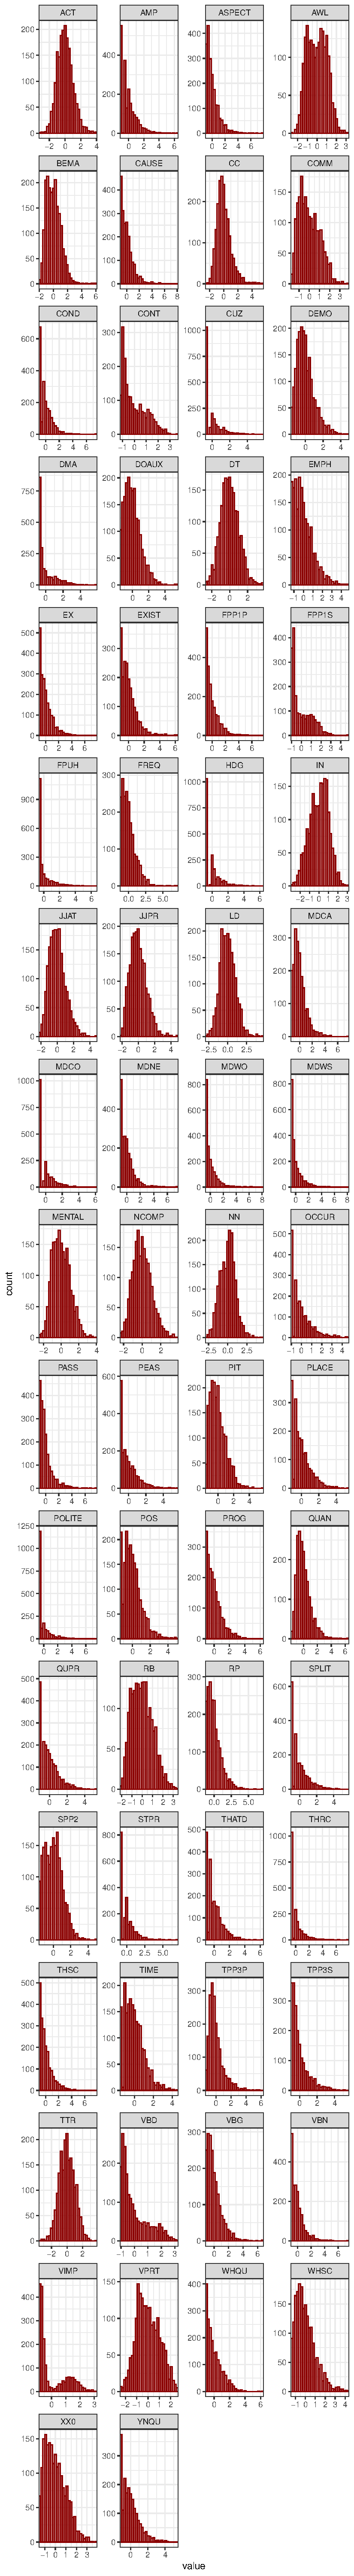
\includegraphics[keepaspectratio]{AppendixE_files/figure-pdf/z-transformed-distributions-1.pdf}}

\begin{Shaded}
\begin{Highlighting}[]
\CommentTok{\#ggsave(here("plots", "TEC{-}zscores{-}HistogramsAllVariablesTEC{-}only.svg"), width = 20, height = 45)}
\end{Highlighting}
\end{Shaded}

\subsection{Signed log transformation}\label{signed-log-transformation}

A signed logarithmic transformation was applied to (further) deskew the
feature distributions (Diwersy, Evert \& Neumann 2014; Neumann \& Evert
2021).

The signed log transformation function was inspired by the SignedLog
function proposed in
https://cran.r-project.org/web/packages/DataVisualizations/DataVisualizations.pdf

\begin{Shaded}
\begin{Highlighting}[]
\CommentTok{\# All features are signed log{-}transformed (note that this is also what Neumann \& Evert 2021 propose)}
\NormalTok{signed.log }\OtherTok{\textless{}{-}} \ControlFlowTok{function}\NormalTok{(x) \{}
  \FunctionTok{sign}\NormalTok{(x) }\SpecialCharTok{*} \FunctionTok{log}\NormalTok{(}\FunctionTok{abs}\NormalTok{(x) }\SpecialCharTok{+} \DecValTok{1}\NormalTok{)}
\NormalTok{  \}}

\NormalTok{TxBzlogcounts }\OtherTok{\textless{}{-}} \FunctionTok{signed.log}\NormalTok{(TxBzcounts) }\CommentTok{\# Standardise first, then signed log transform}

\CommentTok{\#saveRDS(TxBzlogcounts, here("data", "processed", "TxBzlogcounts.rds")) \# Last saved 6 March 2024}
\end{Highlighting}
\end{Shaded}

The new feature distributions are visualised below.

\begin{Shaded}
\begin{Highlighting}[]
\NormalTok{TxBzlogcounts }\SpecialCharTok{|\textgreater{}} 
  \FunctionTok{as.data.frame}\NormalTok{() }\SpecialCharTok{|\textgreater{}}  
  \FunctionTok{gather}\NormalTok{() }\SpecialCharTok{|\textgreater{}}  \CommentTok{\# This function from tidyr converts a selection of variables into two variables: a key and a value. The key contains the names of the original variable and the value the data. This means we can then use the facet\_wrap function from ggplot2}
  \FunctionTok{ggplot}\NormalTok{(}\FunctionTok{aes}\NormalTok{(value, }\FunctionTok{after\_stat}\NormalTok{(density))) }\SpecialCharTok{+}
  \FunctionTok{theme\_bw}\NormalTok{() }\SpecialCharTok{+}
  \FunctionTok{facet\_wrap}\NormalTok{(}\SpecialCharTok{\textasciitilde{}}\NormalTok{ key, }\AttributeTok{scales =} \StringTok{"free"}\NormalTok{, }\AttributeTok{ncol =} \DecValTok{4}\NormalTok{) }\SpecialCharTok{+}
  \FunctionTok{scale\_x\_continuous}\NormalTok{(}\AttributeTok{expand=}\FunctionTok{c}\NormalTok{(}\DecValTok{0}\NormalTok{,}\DecValTok{0}\NormalTok{)) }\SpecialCharTok{+}
  \FunctionTok{scale\_y\_continuous}\NormalTok{(}\AttributeTok{limits =} \FunctionTok{c}\NormalTok{(}\DecValTok{0}\NormalTok{,}\ConstantTok{NA}\NormalTok{)) }\SpecialCharTok{+}
  \FunctionTok{geom\_histogram}\NormalTok{(}\AttributeTok{bins =} \DecValTok{30}\NormalTok{, }\AttributeTok{colour=} \StringTok{"black"}\NormalTok{, }\AttributeTok{fill =} \StringTok{"grey"}\NormalTok{) }\SpecialCharTok{+}
  \FunctionTok{geom\_density}\NormalTok{(}\AttributeTok{colour =} \StringTok{"darkred"}\NormalTok{, }\AttributeTok{weight =} \DecValTok{2}\NormalTok{, }\AttributeTok{fill=}\StringTok{"darkred"}\NormalTok{, }\AttributeTok{alpha =}\NormalTok{ .}\DecValTok{4}\NormalTok{)}
\end{Highlighting}
\end{Shaded}

\pandocbounded{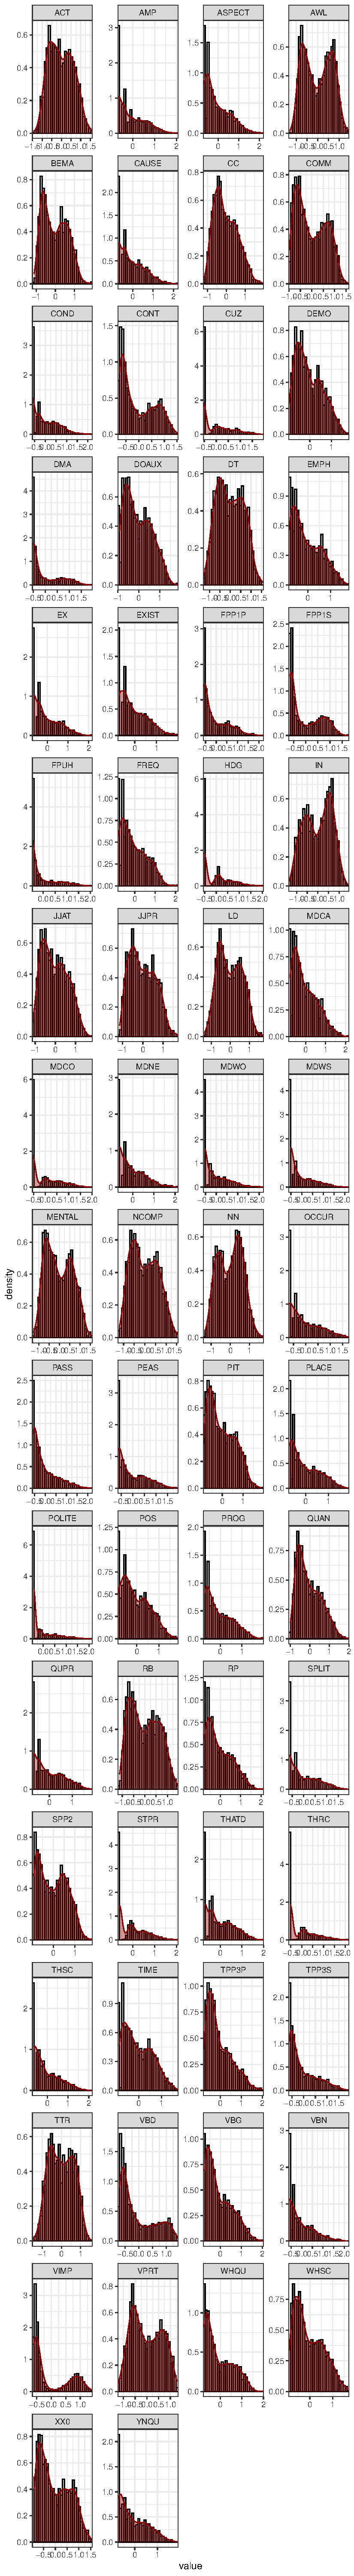
\includegraphics[keepaspectratio]{AppendixE_files/figure-pdf/signed.log.transformation-distributions-1.pdf}}

\begin{Shaded}
\begin{Highlighting}[]
\CommentTok{\#ggsave(here("plots", "DensityPlotsAllVariablesSignedLog{-}TEC{-}only.svg"), width = 15, height = 49)}
\end{Highlighting}
\end{Shaded}

The following correlation plots serve to illustrate the effect of the
variable transformations performed in the above chunks.

Example feature distributions before transformations:

\begin{Shaded}
\begin{Highlighting}[]
\CommentTok{\# This is a slightly amended version of the PerformanceAnalytics::chart.Correlation() function. It simply removes the significance stars that are meaningless with this many data points (see commented out lines below)}

\NormalTok{chart.Correlation.nostars }\OtherTok{\textless{}{-}} \ControlFlowTok{function}\NormalTok{ (R, }\AttributeTok{histogram =} \ConstantTok{TRUE}\NormalTok{, }\AttributeTok{method =} \FunctionTok{c}\NormalTok{(}\StringTok{"pearson"}\NormalTok{, }\StringTok{"kendall"}\NormalTok{, }\StringTok{"spearman"}\NormalTok{), ...) \{}
\NormalTok{  x }\OtherTok{=} \FunctionTok{checkData}\NormalTok{(R, }\AttributeTok{method =} \StringTok{"matrix"}\NormalTok{)}
  \ControlFlowTok{if}\NormalTok{ (}\FunctionTok{missing}\NormalTok{(method)) }
\NormalTok{    method }\OtherTok{=}\NormalTok{ method[}\DecValTok{1}\NormalTok{]}
\NormalTok{  panel.cor }\OtherTok{\textless{}{-}} \ControlFlowTok{function}\NormalTok{(x, y, }\AttributeTok{digits =} \DecValTok{2}\NormalTok{, }\AttributeTok{prefix =} \StringTok{""}\NormalTok{, }\AttributeTok{use =} \StringTok{"pairwise.complete.obs"}\NormalTok{, }\AttributeTok{method =} \StringTok{"pearson"}\NormalTok{, cex.cor, ...) \{}
\NormalTok{    usr }\OtherTok{\textless{}{-}} \FunctionTok{par}\NormalTok{(}\StringTok{"usr"}\NormalTok{)}
    \FunctionTok{on.exit}\NormalTok{(}\FunctionTok{par}\NormalTok{(usr))}
    \FunctionTok{par}\NormalTok{(}\AttributeTok{usr =} \FunctionTok{c}\NormalTok{(}\DecValTok{0}\NormalTok{, }\DecValTok{1}\NormalTok{, }\DecValTok{0}\NormalTok{, }\DecValTok{1}\NormalTok{))}
\NormalTok{    r }\OtherTok{\textless{}{-}} \FunctionTok{cor}\NormalTok{(x, y, }\AttributeTok{use =}\NormalTok{ use, }\AttributeTok{method =}\NormalTok{ method)}
\NormalTok{    txt }\OtherTok{\textless{}{-}} \FunctionTok{format}\NormalTok{(}\FunctionTok{c}\NormalTok{(r, }\FloatTok{0.123456789}\NormalTok{), }\AttributeTok{digits =}\NormalTok{ digits)[}\DecValTok{1}\NormalTok{]}
\NormalTok{    txt }\OtherTok{\textless{}{-}} \FunctionTok{paste}\NormalTok{(prefix, txt, }\AttributeTok{sep =} \StringTok{""}\NormalTok{)}
    \ControlFlowTok{if}\NormalTok{ (}\FunctionTok{missing}\NormalTok{(cex.cor)) }
\NormalTok{      cex }\OtherTok{\textless{}{-}} \FloatTok{0.8}\SpecialCharTok{/}\FunctionTok{strwidth}\NormalTok{(txt)}
\NormalTok{    test }\OtherTok{\textless{}{-}} \FunctionTok{cor.test}\NormalTok{(}\FunctionTok{as.numeric}\NormalTok{(x), }\FunctionTok{as.numeric}\NormalTok{(y), }\AttributeTok{method =}\NormalTok{ method)}
    \CommentTok{\# Signif \textless{}{-} symnum(test$p.value, corr = FALSE, na = FALSE, }
    \CommentTok{\#                  cutpoints = c(0, 0.001, 0.01, 0.05, 0.1, 1), symbols = c("***", }
    \CommentTok{\#                                                                           "**", "*", ".", " "))}
    \FunctionTok{text}\NormalTok{(}\FloatTok{0.5}\NormalTok{, }\FloatTok{0.5}\NormalTok{, txt, }\AttributeTok{cex =}\NormalTok{ cex }\SpecialCharTok{*}\NormalTok{ (}\FunctionTok{abs}\NormalTok{(r) }\SpecialCharTok{+} \FloatTok{0.3}\NormalTok{)}\SpecialCharTok{/}\FloatTok{1.3}\NormalTok{)}
    \CommentTok{\# text(0.8, 0.8, Signif, cex = cex, col = 2)}
\NormalTok{  \}}
\NormalTok{  f }\OtherTok{\textless{}{-}} \ControlFlowTok{function}\NormalTok{(t) \{}
    \FunctionTok{dnorm}\NormalTok{(t, }\AttributeTok{mean =} \FunctionTok{mean}\NormalTok{(x), }\AttributeTok{sd =} \FunctionTok{sd.xts}\NormalTok{(x))}
\NormalTok{  \}}
\NormalTok{  dotargs }\OtherTok{\textless{}{-}} \FunctionTok{list}\NormalTok{(...)}
\NormalTok{  dotargs}\SpecialCharTok{$}\NormalTok{method }\OtherTok{\textless{}{-}} \ConstantTok{NULL}
  \FunctionTok{rm}\NormalTok{(method)}
\NormalTok{  hist.panel }\OtherTok{=} \ControlFlowTok{function}\NormalTok{(x, }\AttributeTok{... =} \ConstantTok{NULL}\NormalTok{) \{}
    \FunctionTok{par}\NormalTok{(}\AttributeTok{new =} \ConstantTok{TRUE}\NormalTok{)}
    \FunctionTok{hist}\NormalTok{(x, }\AttributeTok{col =} \StringTok{"light gray"}\NormalTok{, }\AttributeTok{probability =} \ConstantTok{TRUE}\NormalTok{, }
         \AttributeTok{axes =} \ConstantTok{FALSE}\NormalTok{, }\AttributeTok{main =} \StringTok{""}\NormalTok{, }\AttributeTok{breaks =} \StringTok{"FD"}\NormalTok{)}
    \FunctionTok{lines}\NormalTok{(}\FunctionTok{density}\NormalTok{(x, }\AttributeTok{na.rm =} \ConstantTok{TRUE}\NormalTok{), }\AttributeTok{col =} \StringTok{"red"}\NormalTok{, }\AttributeTok{lwd =} \DecValTok{1}\NormalTok{)}
    \FunctionTok{rug}\NormalTok{(x)}
\NormalTok{  \}}
  \ControlFlowTok{if}\NormalTok{ (histogram) }
    \FunctionTok{pairs}\NormalTok{(x, }\AttributeTok{gap =} \DecValTok{0}\NormalTok{, }\AttributeTok{lower.panel =}\NormalTok{ panel.smooth, }\AttributeTok{upper.panel =}\NormalTok{ panel.cor, }
          \AttributeTok{diag.panel =}\NormalTok{ hist.panel)}
  \ControlFlowTok{else} \FunctionTok{pairs}\NormalTok{(x, }\AttributeTok{gap =} \DecValTok{0}\NormalTok{, }\AttributeTok{lower.panel =}\NormalTok{ panel.smooth, }\AttributeTok{upper.panel =}\NormalTok{ panel.cor)}
\NormalTok{\}}

\CommentTok{\# Example plot without any variable transformation}
\NormalTok{example1 }\OtherTok{\textless{}{-}}\NormalTok{ TxBcounts }\SpecialCharTok{|\textgreater{}} 
  \FunctionTok{select}\NormalTok{(NN,PROG,SPLIT,ACT,FPP1S)}

\CommentTok{\#png(here("plots", "CorrChart{-}TEC{-}examples{-}normedcounts.png"), width = 20, height = 20, units = "cm", res = 300)}
\FunctionTok{chart.Correlation.nostars}\NormalTok{(example1, }\AttributeTok{histogram=}\ConstantTok{TRUE}\NormalTok{, }\AttributeTok{pch=}\DecValTok{19}\NormalTok{)}
\end{Highlighting}
\end{Shaded}

\pandocbounded{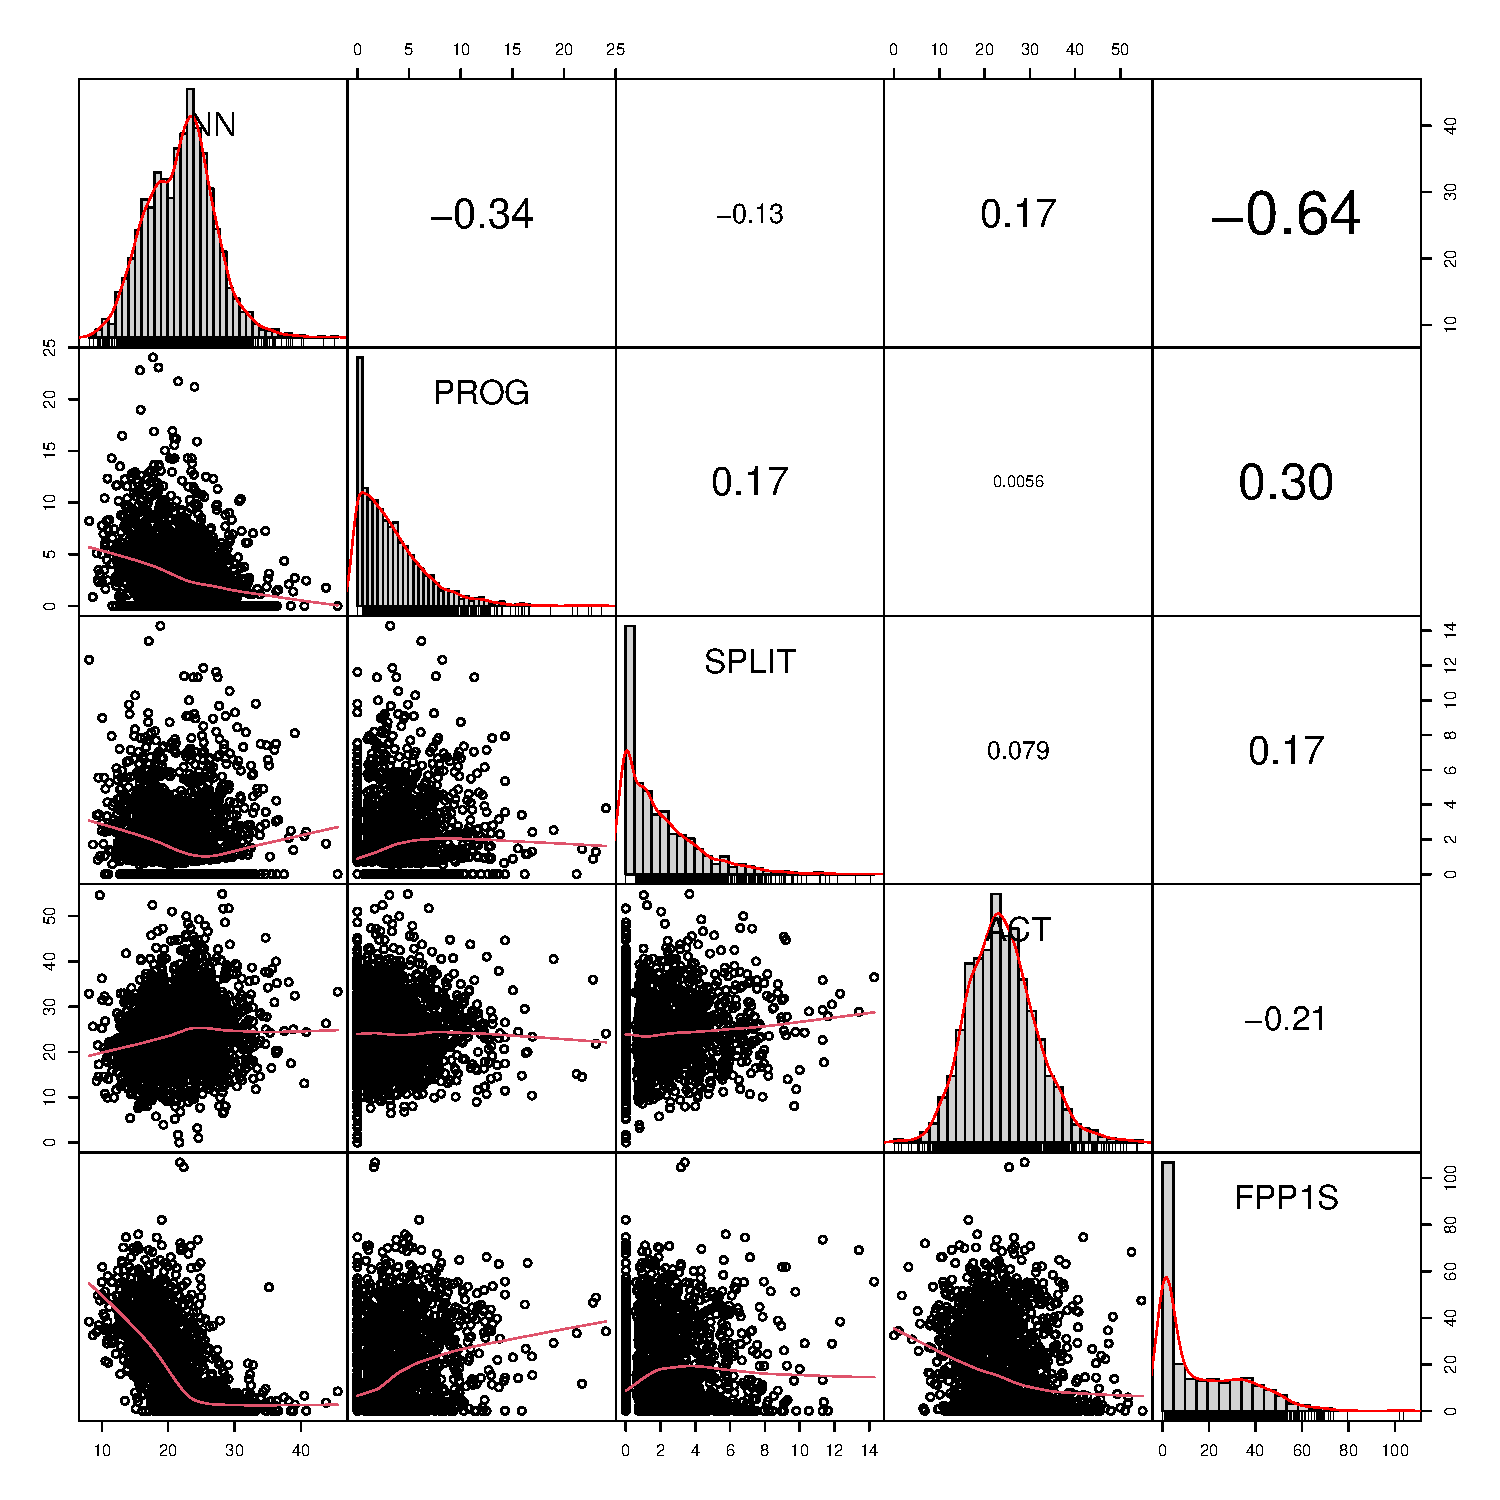
\includegraphics[keepaspectratio]{AppendixE_files/figure-pdf/example-correlation-plots-1.pdf}}

\begin{Shaded}
\begin{Highlighting}[]
\CommentTok{\#dev.off()}
\end{Highlighting}
\end{Shaded}

Example feature distributions after transformations:

\begin{Shaded}
\begin{Highlighting}[]
\CommentTok{\# Example plot with transformed variables}
\NormalTok{example2 }\OtherTok{\textless{}{-}}\NormalTok{ TxBzlogcounts }\SpecialCharTok{|\textgreater{}} 
  \FunctionTok{as.data.frame}\NormalTok{() }\SpecialCharTok{|\textgreater{}}  
  \FunctionTok{select}\NormalTok{(NN,PROG,SPLIT,ACT,FPP1S)}

\CommentTok{\#png(here("plots", "CorrChart{-}TEC{-}examples{-}zsignedlogcounts.png"), width = 20, height = 20, units = "cm", res = 300)}
\FunctionTok{chart.Correlation.nostars}\NormalTok{(example2, }\AttributeTok{histogram=}\ConstantTok{TRUE}\NormalTok{, }\AttributeTok{pch=}\DecValTok{19}\NormalTok{)}
\end{Highlighting}
\end{Shaded}

\pandocbounded{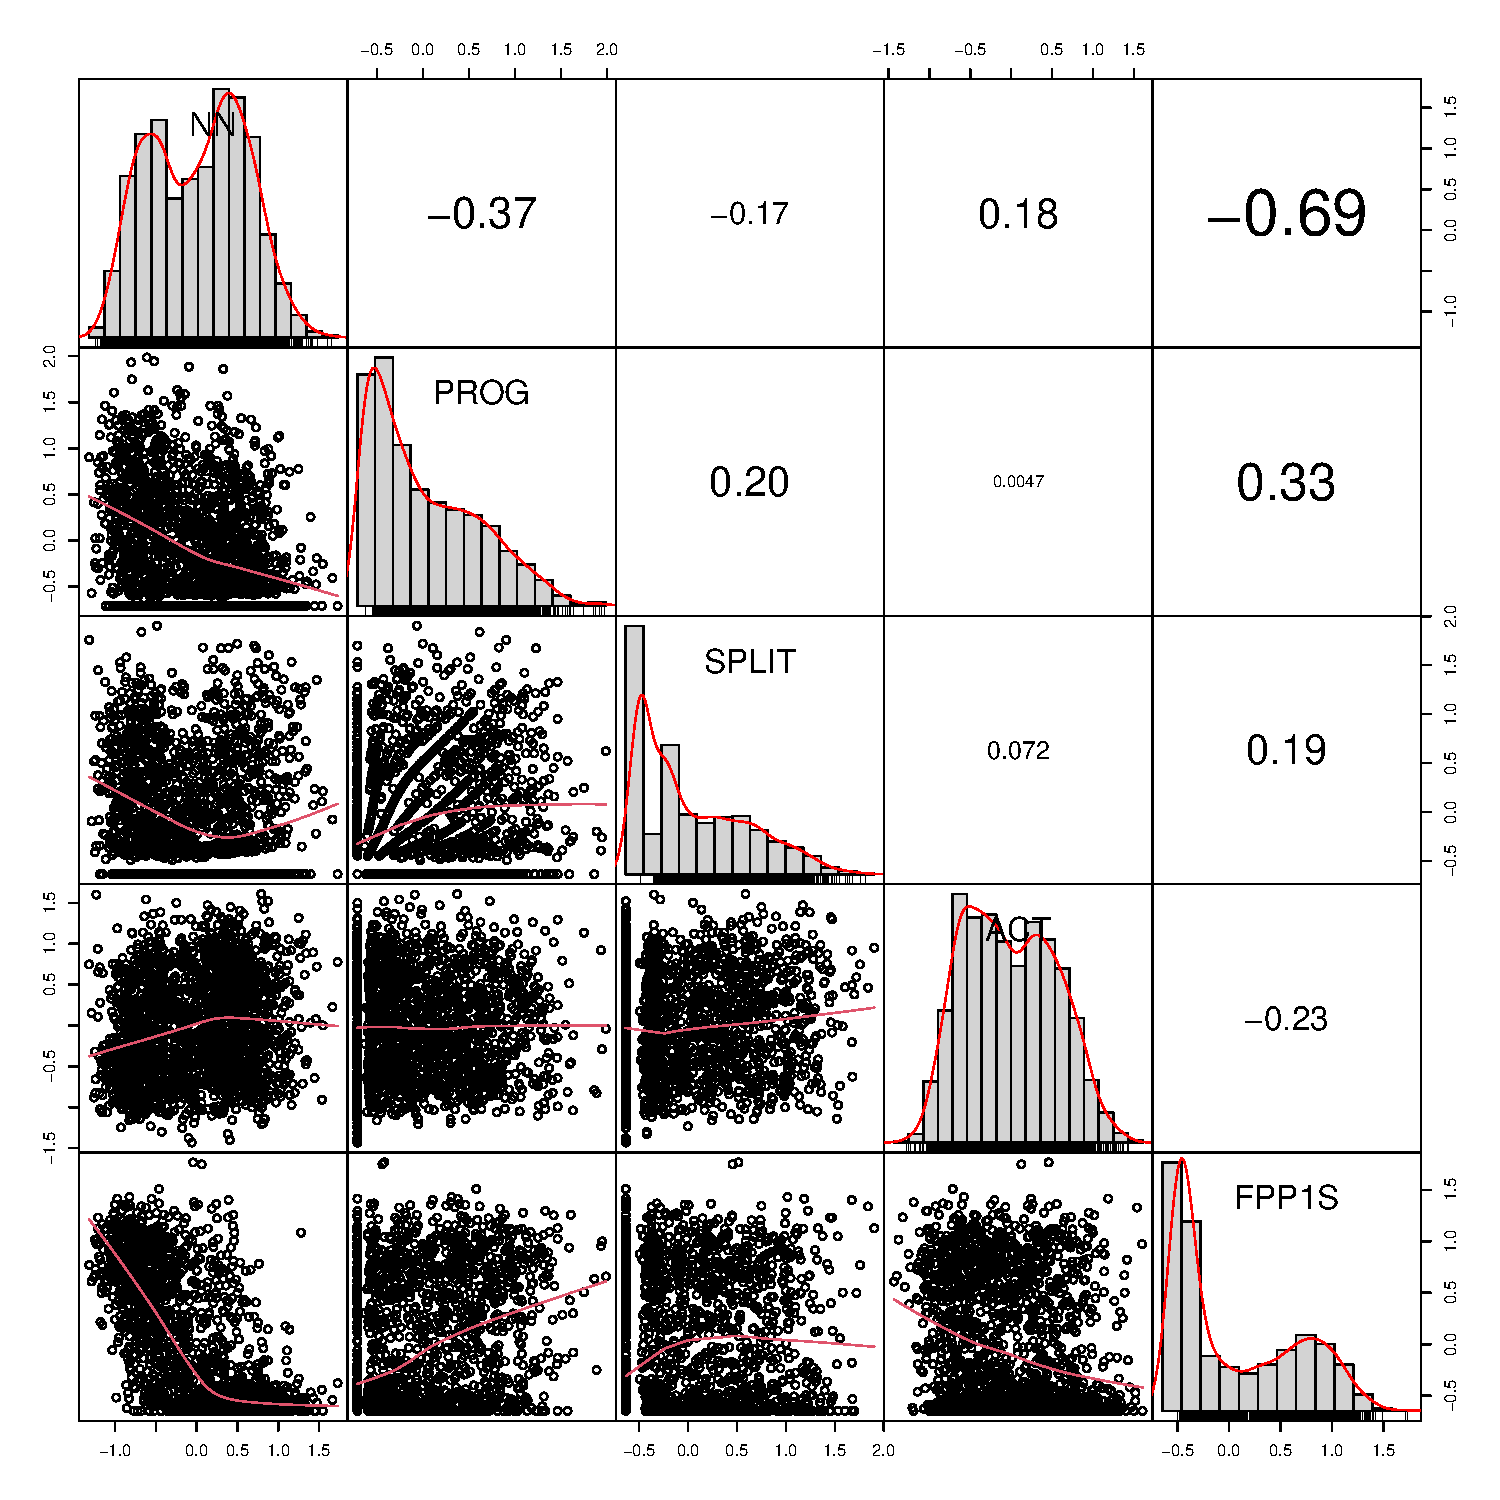
\includegraphics[keepaspectratio]{AppendixE_files/figure-pdf/example-correlation-plots2-1.pdf}}

\begin{Shaded}
\begin{Highlighting}[]
\CommentTok{\#dev.off()}
\end{Highlighting}
\end{Shaded}

\subsection{Feature correlations}\label{feature-correlations}

The correlations of the transformed feature frequencies can be
visualised in the form of a heatmap. Negative correlations are rendered
in blue, whereas positive ones are in red.

\begin{Shaded}
\begin{Highlighting}[]
\CommentTok{\# Simple heatmap in base R (inspired by Stephanie Evert\textquotesingle{}s SIGIL code)}
\NormalTok{cor.colours }\OtherTok{\textless{}{-}} \FunctionTok{c}\NormalTok{(}
  \FunctionTok{hsv}\NormalTok{(}\AttributeTok{h=}\DecValTok{2}\SpecialCharTok{/}\DecValTok{3}\NormalTok{, }\AttributeTok{v=}\DecValTok{1}\NormalTok{, }\AttributeTok{s=}\NormalTok{(}\DecValTok{10}\SpecialCharTok{:}\DecValTok{1}\NormalTok{)}\SpecialCharTok{/}\DecValTok{10}\NormalTok{), }\CommentTok{\# blue = negative correlation }
  \FunctionTok{rgb}\NormalTok{(}\DecValTok{1}\NormalTok{,}\DecValTok{1}\NormalTok{,}\DecValTok{1}\NormalTok{), }\CommentTok{\# white = no correlation }
  \FunctionTok{hsv}\NormalTok{(}\AttributeTok{h=}\DecValTok{0}\NormalTok{, }\AttributeTok{v=}\DecValTok{1}\NormalTok{, }\AttributeTok{s=}\NormalTok{(}\DecValTok{1}\SpecialCharTok{:}\DecValTok{10}\SpecialCharTok{/}\DecValTok{10}\NormalTok{))) }\CommentTok{\# red = positive correlation}

\CommentTok{\#png(here("plots", "heatmapzlogcounts{-}TEC{-}only.png"), width = 30, height= 30, units = "cm", res = 300)}
\FunctionTok{heatmap}\NormalTok{(}\FunctionTok{cor}\NormalTok{(TxBzlogcounts), }
        \AttributeTok{symm=}\ConstantTok{TRUE}\NormalTok{, }
        \AttributeTok{zlim=}\FunctionTok{c}\NormalTok{(}\SpecialCharTok{{-}}\DecValTok{1}\NormalTok{,}\DecValTok{1}\NormalTok{), }
        \AttributeTok{col=}\NormalTok{cor.colours, }
        \AttributeTok{margins=}\FunctionTok{c}\NormalTok{(}\DecValTok{0}\NormalTok{,}\DecValTok{0}\NormalTok{))}
\end{Highlighting}
\end{Shaded}

\pandocbounded{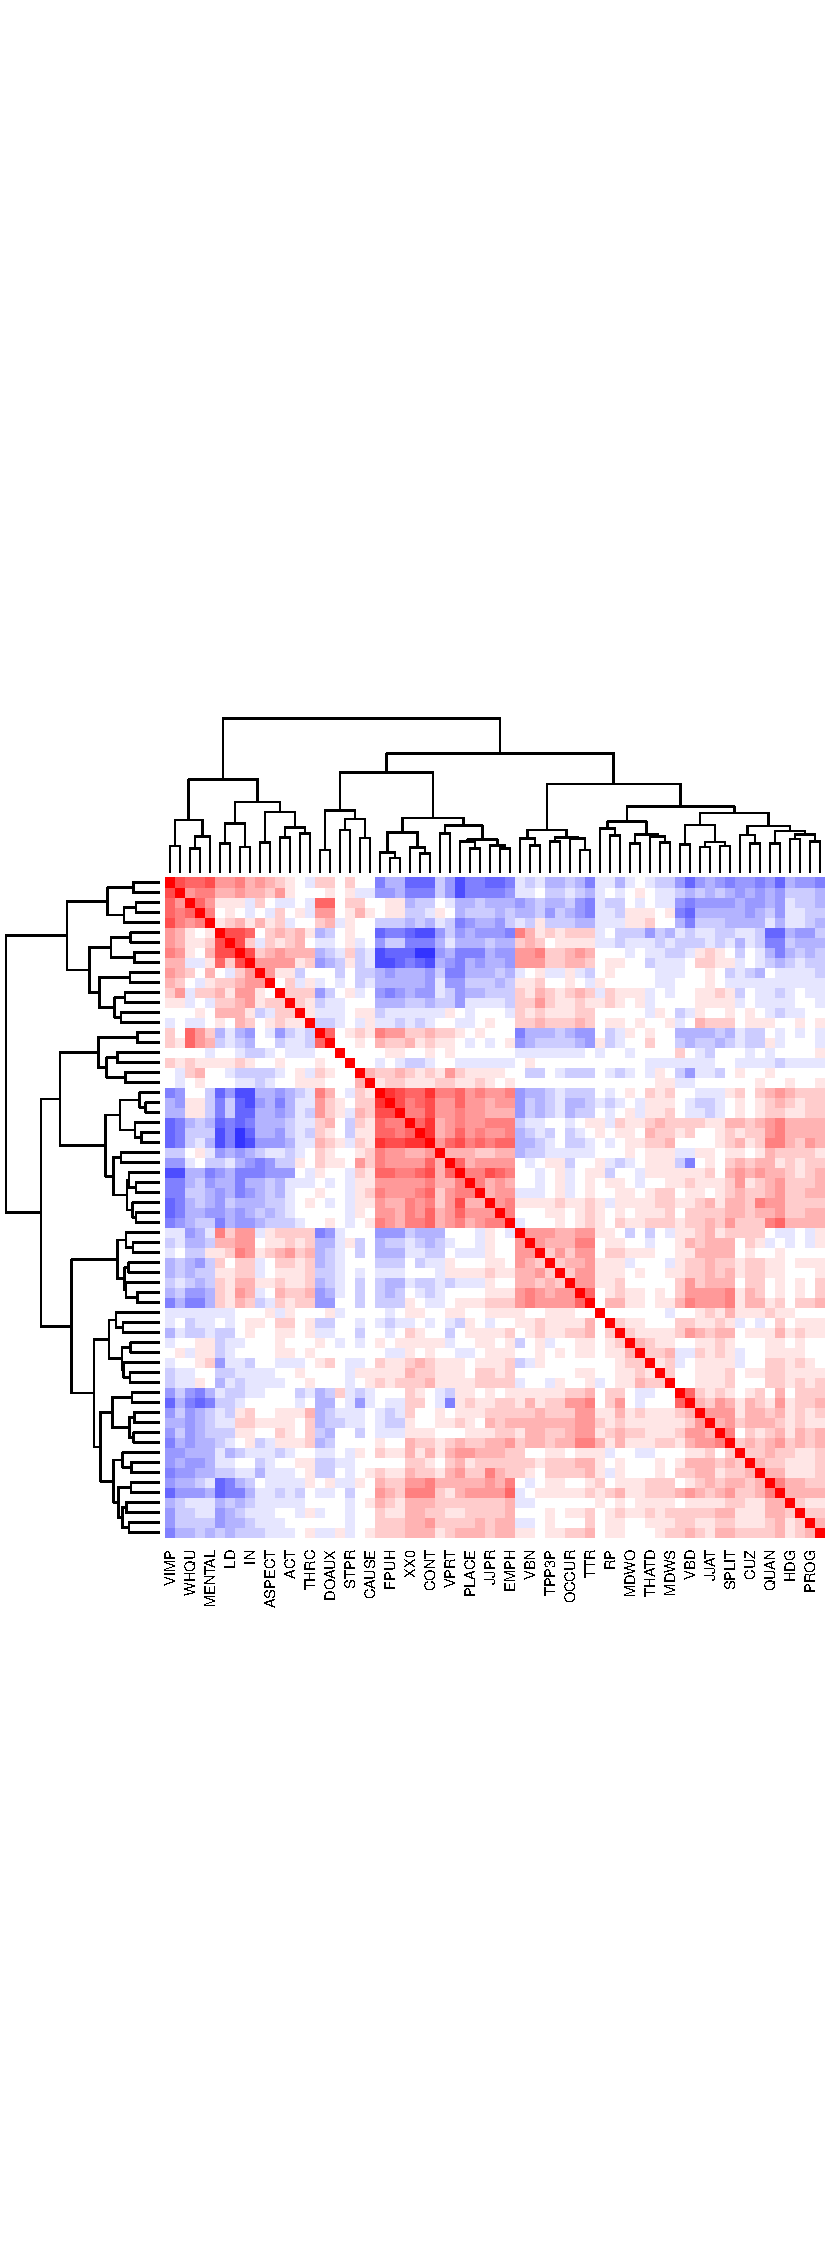
\includegraphics[keepaspectratio]{AppendixE_files/figure-pdf/heatmap-1.pdf}}

\begin{Shaded}
\begin{Highlighting}[]
\CommentTok{\#dev.off()}

\CommentTok{\# Calculate the sum of all the words in the tagged texts of the TEC}
\NormalTok{totalwords }\OtherTok{\textless{}{-}}\NormalTok{ TxBcounts }\SpecialCharTok{|\textgreater{}}  
  \FunctionTok{select}\NormalTok{(Words) }\SpecialCharTok{|\textgreater{}} 
  \FunctionTok{sum}\NormalTok{() }\SpecialCharTok{|\textgreater{}} 
  \FunctionTok{format}\NormalTok{(}\AttributeTok{big.mark=}\StringTok{","}\NormalTok{)}
\end{Highlighting}
\end{Shaded}

\section{Composition of TEC
texts/files}\label{composition-of-tec-textsfiles}

These figures and tables provide summary statistics on the texts/files
of the TEC that were entered in the multi-dimensional model of
intra-textbook linguistic variation. In total, the TEC texts entered
amounted to 1,693,650 words.

\begin{Shaded}
\begin{Highlighting}[]
\NormalTok{metadata }\OtherTok{\textless{}{-}}\NormalTok{ TxBcounts }\SpecialCharTok{|\textgreater{}}  
  \FunctionTok{select}\NormalTok{(Filename, Country, Series, Level, Register, Words) }\SpecialCharTok{|\textgreater{}}  
  \FunctionTok{mutate}\NormalTok{(}\AttributeTok{Volume =} \FunctionTok{paste}\NormalTok{(Series, Level)) }\SpecialCharTok{|\textgreater{}}  
  \FunctionTok{mutate}\NormalTok{(}\AttributeTok{Volume =} \FunctionTok{fct\_rev}\NormalTok{(Volume)) }\SpecialCharTok{|\textgreater{}}  
  \FunctionTok{mutate}\NormalTok{(}\AttributeTok{Volume =} \FunctionTok{fct\_reorder}\NormalTok{(Volume, }\FunctionTok{as.numeric}\NormalTok{(Level))) }\SpecialCharTok{|\textgreater{}}  
  \FunctionTok{group\_by}\NormalTok{(Volume) }\SpecialCharTok{|\textgreater{}}  
  \FunctionTok{mutate}\NormalTok{(}\AttributeTok{wordcount =} \FunctionTok{sum}\NormalTok{(Words)) }\SpecialCharTok{|\textgreater{}}  
  \FunctionTok{ungroup}\NormalTok{() }\SpecialCharTok{|\textgreater{}}  
  \FunctionTok{distinct}\NormalTok{(Volume, }\AttributeTok{.keep\_all =} \ConstantTok{TRUE}\NormalTok{)}

\CommentTok{\# Plot for book}
\NormalTok{metadata2 }\OtherTok{\textless{}{-}}\NormalTok{ TxBcounts }\SpecialCharTok{|\textgreater{}}  
  \FunctionTok{select}\NormalTok{(Country, Series, Level, Register, Words) }\SpecialCharTok{|\textgreater{}}  
  \FunctionTok{mutate}\NormalTok{(}\AttributeTok{Volume =} \FunctionTok{paste}\NormalTok{(Series, Level)) }\SpecialCharTok{|\textgreater{}}  
  \FunctionTok{mutate}\NormalTok{(}\AttributeTok{Volume =} \FunctionTok{fct\_rev}\NormalTok{(Volume)) }\SpecialCharTok{|\textgreater{}}  
  \CommentTok{\#mutate(Volume = fct\_reorder(Volume, as.numeric(Level))) |\textgreater{}  }
  \FunctionTok{group\_by}\NormalTok{(Volume, Register) }\SpecialCharTok{|\textgreater{}}  
  \FunctionTok{mutate}\NormalTok{(}\AttributeTok{wordcount =} \FunctionTok{sum}\NormalTok{(Words)) }\SpecialCharTok{|\textgreater{}}  
  \FunctionTok{ungroup}\NormalTok{() }\SpecialCharTok{|\textgreater{}}  
  \FunctionTok{distinct}\NormalTok{(Volume, Register, }\AttributeTok{.keep\_all =} \ConstantTok{TRUE}\NormalTok{)}

\CommentTok{\# This is the palette created above on the basis of the suffrager pakcage (but without needed to install the package)}
\NormalTok{palette }\OtherTok{\textless{}{-}} \FunctionTok{c}\NormalTok{(}\StringTok{"\#BD241E"}\NormalTok{, }\StringTok{"\#A18A33"}\NormalTok{, }\StringTok{"\#15274D"}\NormalTok{, }\StringTok{"\#D54E1E"}\NormalTok{, }\StringTok{"\#EA7E1E"}\NormalTok{, }\StringTok{"\#4C4C4C"}\NormalTok{, }\StringTok{"\#722672"}\NormalTok{, }\StringTok{"\#F9B921"}\NormalTok{, }\StringTok{"\#267226"}\NormalTok{)}

\NormalTok{PlotSp }\OtherTok{\textless{}{-}}\NormalTok{ metadata2 }\SpecialCharTok{|\textgreater{}}  
  \FunctionTok{filter}\NormalTok{(Country}\SpecialCharTok{==}\StringTok{"Spain"}\NormalTok{) }\SpecialCharTok{|\textgreater{}}  
  \CommentTok{\#arrange(Volume) |\textgreater{}  }
  \FunctionTok{ggplot}\NormalTok{(}\FunctionTok{aes}\NormalTok{(}\AttributeTok{x =}\NormalTok{ Volume, }\AttributeTok{y =}\NormalTok{ wordcount, }\AttributeTok{fill =} \FunctionTok{fct\_rev}\NormalTok{(Register))) }\SpecialCharTok{+} 
    \FunctionTok{geom\_bar}\NormalTok{(}\AttributeTok{stat =} \StringTok{"identity"}\NormalTok{, }\AttributeTok{position =} \StringTok{"stack"}\NormalTok{) }\SpecialCharTok{+}
    \FunctionTok{coord\_flip}\NormalTok{(}\AttributeTok{expand =} \ConstantTok{FALSE}\NormalTok{) }\SpecialCharTok{+} \CommentTok{\# Removes those annoying ticks before each bar label}
    \FunctionTok{theme\_minimal}\NormalTok{() }\SpecialCharTok{+} \FunctionTok{theme}\NormalTok{(}\AttributeTok{legend.position =} \StringTok{"none"}\NormalTok{) }\SpecialCharTok{+}
    \FunctionTok{labs}\NormalTok{(}\AttributeTok{x =} \StringTok{"Spain"}\NormalTok{, }\AttributeTok{y =} \StringTok{"Cumulative word count"}\NormalTok{) }\SpecialCharTok{+}
    \FunctionTok{scale\_fill\_manual}\NormalTok{(}\AttributeTok{values =}\NormalTok{ palette[}\FunctionTok{c}\NormalTok{(}\DecValTok{5}\NormalTok{,}\DecValTok{4}\NormalTok{,}\DecValTok{3}\NormalTok{,}\DecValTok{2}\NormalTok{,}\DecValTok{1}\NormalTok{)], }
                      \AttributeTok{guide =} \FunctionTok{guide\_legend}\NormalTok{(}\AttributeTok{reverse =} \ConstantTok{TRUE}\NormalTok{))}

\NormalTok{PlotGer }\OtherTok{\textless{}{-}}\NormalTok{ metadata2 }\SpecialCharTok{|\textgreater{}}  
  \FunctionTok{filter}\NormalTok{(Country}\SpecialCharTok{==}\StringTok{"Germany"}\NormalTok{) }\SpecialCharTok{|\textgreater{}}  
  \CommentTok{\#arrange(Volume) |\textgreater{}  }
  \FunctionTok{ggplot}\NormalTok{(}\FunctionTok{aes}\NormalTok{(}\AttributeTok{x =}\NormalTok{ Volume, }\AttributeTok{y =}\NormalTok{ wordcount, }\AttributeTok{fill =} \FunctionTok{fct\_rev}\NormalTok{(Register))) }\SpecialCharTok{+} 
    \FunctionTok{geom\_bar}\NormalTok{(}\AttributeTok{stat =} \StringTok{"identity"}\NormalTok{, }\AttributeTok{position =} \StringTok{"stack"}\NormalTok{) }\SpecialCharTok{+}
    \FunctionTok{coord\_flip}\NormalTok{(}\AttributeTok{expand =} \ConstantTok{FALSE}\NormalTok{) }\SpecialCharTok{+}
    \FunctionTok{labs}\NormalTok{(}\AttributeTok{x =} \StringTok{"Germany"}\NormalTok{, }\AttributeTok{y =} \StringTok{""}\NormalTok{) }\SpecialCharTok{+}
    \FunctionTok{scale\_fill\_manual}\NormalTok{(}\AttributeTok{values =}\NormalTok{ palette[}\FunctionTok{c}\NormalTok{(}\DecValTok{5}\NormalTok{,}\DecValTok{4}\NormalTok{,}\DecValTok{3}\NormalTok{,}\DecValTok{2}\NormalTok{,}\DecValTok{1}\NormalTok{)], }\AttributeTok{guide =} \FunctionTok{guide\_legend}\NormalTok{(}\AttributeTok{reverse =} \ConstantTok{TRUE}\NormalTok{)) }\SpecialCharTok{+}
    \FunctionTok{theme\_minimal}\NormalTok{() }\SpecialCharTok{+} \FunctionTok{theme}\NormalTok{(}\AttributeTok{legend.position =} \StringTok{"none"}\NormalTok{)}

\NormalTok{PlotFr }\OtherTok{\textless{}{-}}\NormalTok{ metadata2 }\SpecialCharTok{|\textgreater{}}  
  \FunctionTok{filter}\NormalTok{(Country}\SpecialCharTok{==}\StringTok{"France"}\NormalTok{) }\SpecialCharTok{|\textgreater{}}  
  \CommentTok{\#arrange(Volume) |\textgreater{}  }
  \FunctionTok{ggplot}\NormalTok{(}\FunctionTok{aes}\NormalTok{(}\AttributeTok{x =}\NormalTok{ Volume, }\AttributeTok{y =}\NormalTok{ wordcount, }\AttributeTok{fill =} \FunctionTok{fct\_rev}\NormalTok{(Register))) }\SpecialCharTok{+} 
    \FunctionTok{geom\_bar}\NormalTok{(}\AttributeTok{stat =} \StringTok{"identity"}\NormalTok{, }\AttributeTok{position =} \StringTok{"stack"}\NormalTok{) }\SpecialCharTok{+}
    \FunctionTok{coord\_flip}\NormalTok{(}\AttributeTok{expand =} \ConstantTok{FALSE}\NormalTok{) }\SpecialCharTok{+}
    \FunctionTok{labs}\NormalTok{(}\AttributeTok{x =} \StringTok{"France"}\NormalTok{, }\AttributeTok{y  =} \StringTok{""}\NormalTok{, }\AttributeTok{fill =} \StringTok{"Register subcorpus"}\NormalTok{) }\SpecialCharTok{+}
    \FunctionTok{scale\_fill\_manual}\NormalTok{(}\AttributeTok{values =}\NormalTok{ palette[}\FunctionTok{c}\NormalTok{(}\DecValTok{5}\NormalTok{,}\DecValTok{4}\NormalTok{,}\DecValTok{3}\NormalTok{,}\DecValTok{2}\NormalTok{,}\DecValTok{1}\NormalTok{)], }\AttributeTok{guide =} \FunctionTok{guide\_legend}\NormalTok{(}\AttributeTok{reverse =} \ConstantTok{TRUE}\NormalTok{, }\AttributeTok{legend.hjust =} \DecValTok{0}\NormalTok{)) }\SpecialCharTok{+}
    \FunctionTok{theme\_minimal}\NormalTok{() }\SpecialCharTok{+} \FunctionTok{theme}\NormalTok{(}\AttributeTok{legend.position =} \StringTok{"top"}\NormalTok{, }\AttributeTok{legend.justification =} \StringTok{"left"}\NormalTok{)}

\FunctionTok{library}\NormalTok{(patchwork)}

\NormalTok{PlotFr }\SpecialCharTok{/}
\NormalTok{PlotGer }\SpecialCharTok{/}
\NormalTok{PlotSp}
\end{Highlighting}
\end{Shaded}

\pandocbounded{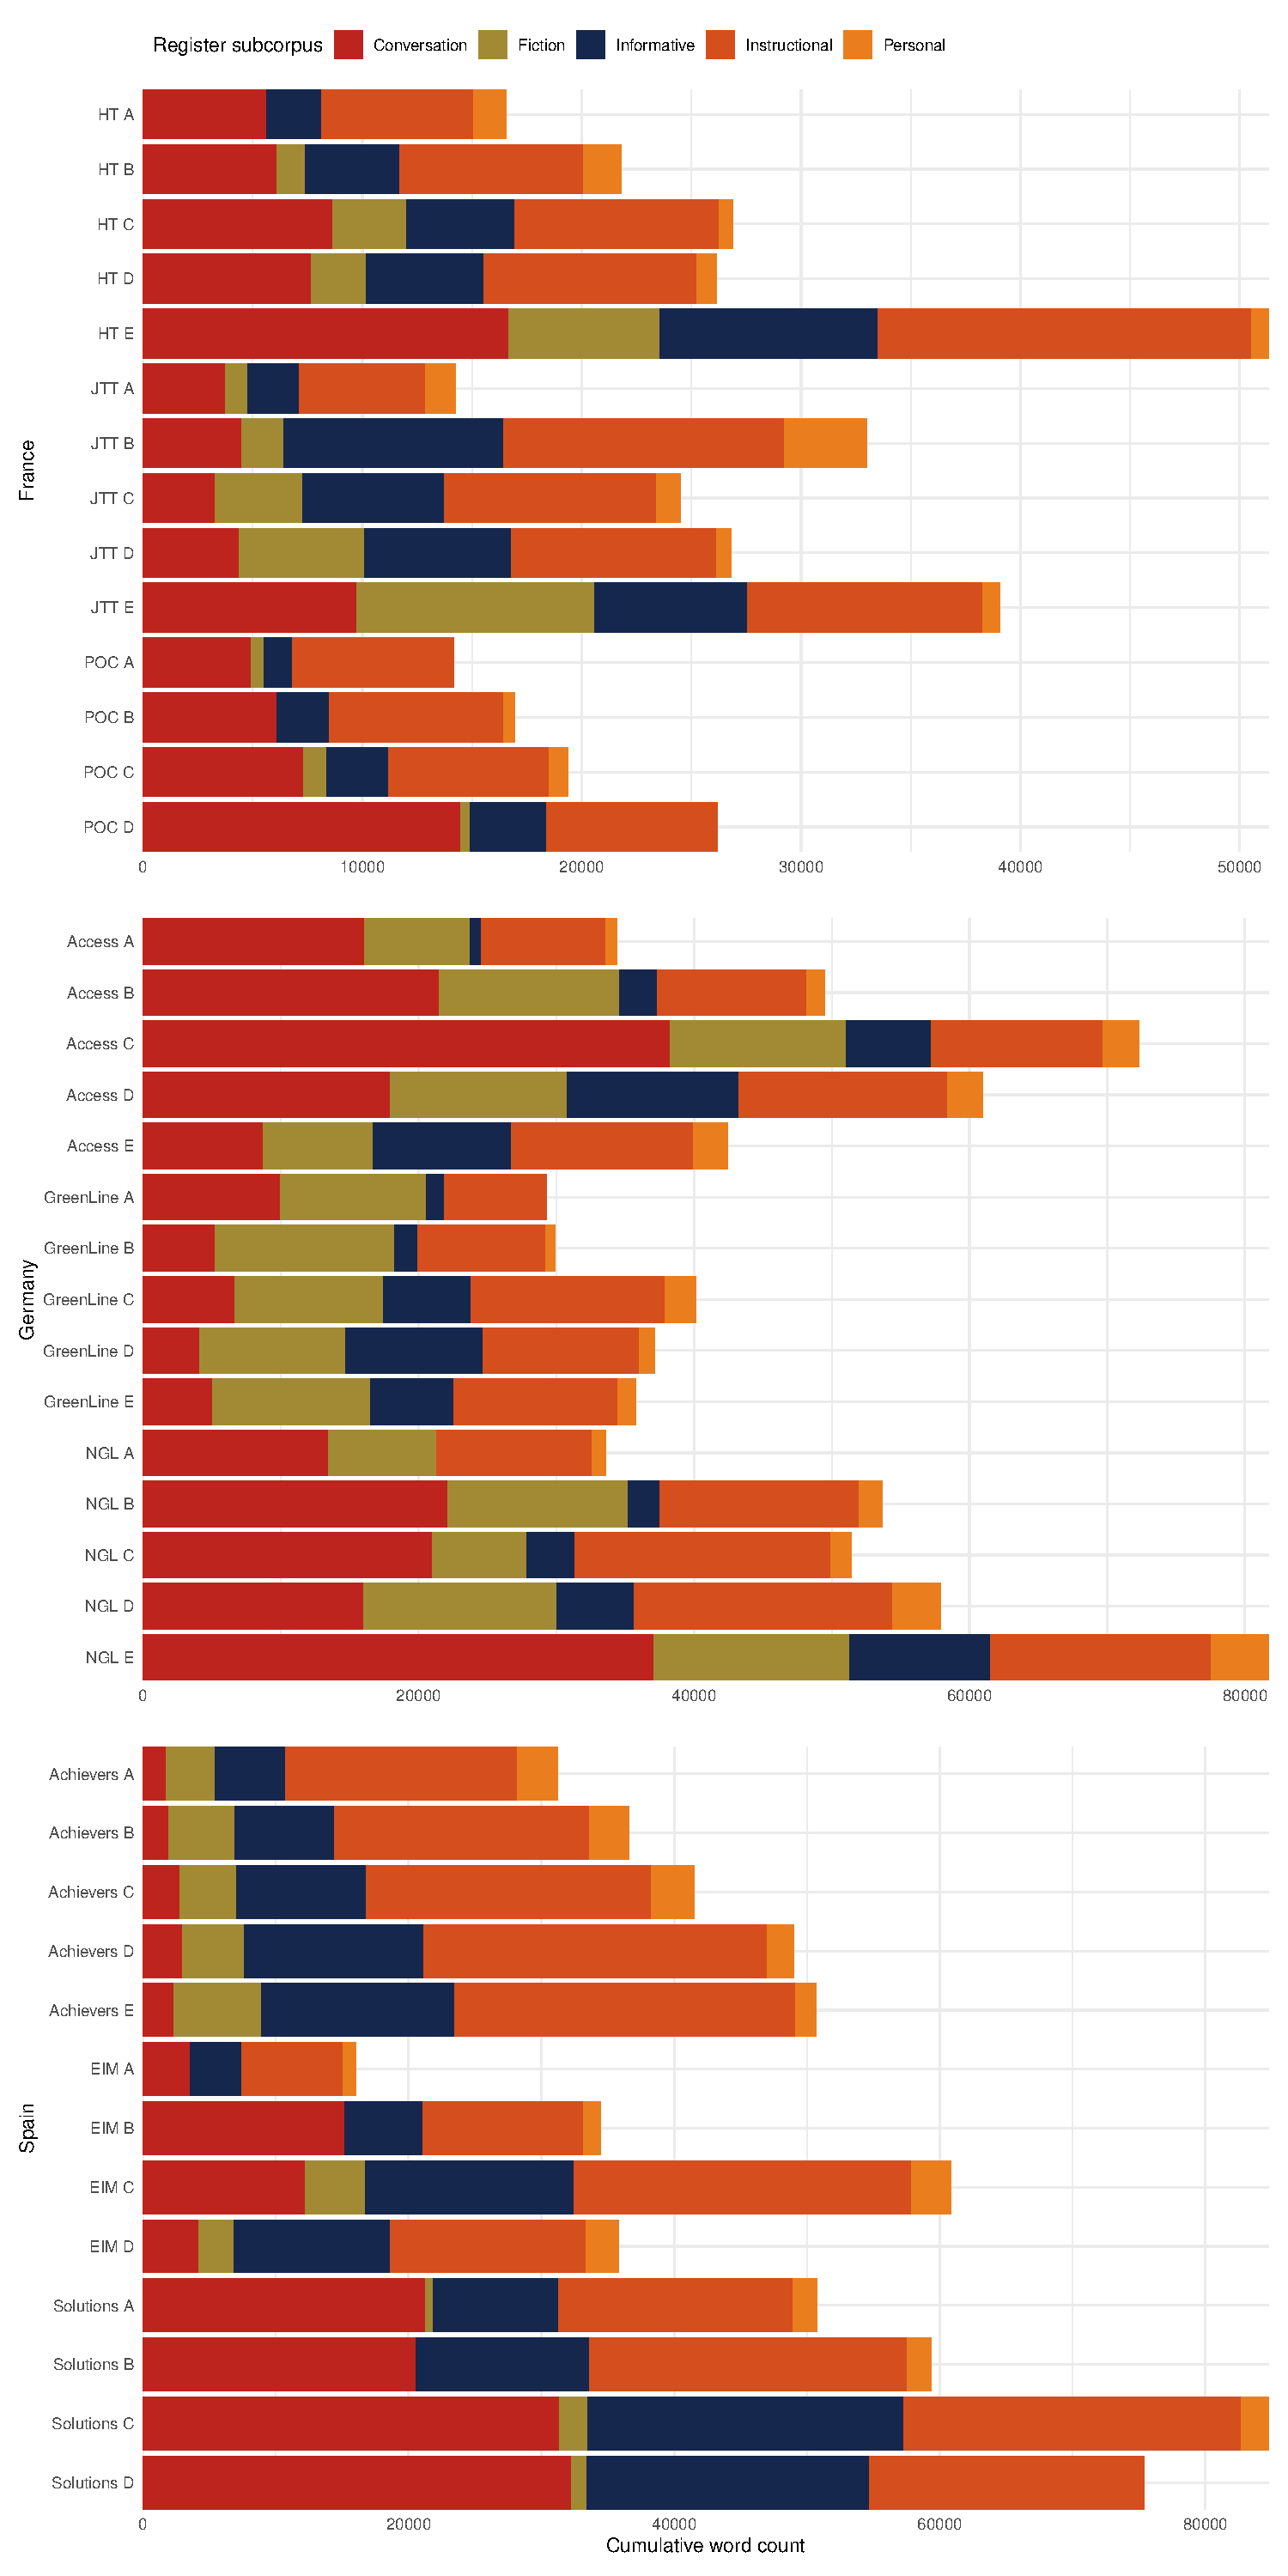
\includegraphics[keepaspectratio]{AppendixE_files/figure-pdf/TEC-metadata-1.pdf}}

\begin{Shaded}
\begin{Highlighting}[]
\CommentTok{\#ggsave(here("plots", "TEC{-}T\_wordcounts\_book.svg"), width = 8, height = 12)}
\end{Highlighting}
\end{Shaded}

The following table provides information about the proportion of
instructional language featured in each textbook series.

\begin{Shaded}
\begin{Highlighting}[]
\NormalTok{metadataInstr }\OtherTok{\textless{}{-}}\NormalTok{ TxBcounts }\SpecialCharTok{|\textgreater{}}  
  \FunctionTok{select}\NormalTok{(Country, Series, Level, Register, Words) }\SpecialCharTok{|\textgreater{}}  
  \FunctionTok{filter}\NormalTok{(Register}\SpecialCharTok{==}\StringTok{"Instructional"}\NormalTok{) }\SpecialCharTok{|\textgreater{}}  
  \FunctionTok{mutate}\NormalTok{(}\AttributeTok{Volume =} \FunctionTok{paste}\NormalTok{(Series, Register)) }\SpecialCharTok{|\textgreater{}}  
  \FunctionTok{mutate}\NormalTok{(}\AttributeTok{Volume =} \FunctionTok{fct\_rev}\NormalTok{(Volume)) }\SpecialCharTok{|\textgreater{}}  
  \FunctionTok{mutate}\NormalTok{(}\AttributeTok{Volume =} \FunctionTok{fct\_reorder}\NormalTok{(Volume, }\FunctionTok{as.numeric}\NormalTok{(Level))) }\SpecialCharTok{|\textgreater{}}  
  \FunctionTok{group\_by}\NormalTok{(Volume, Register) }\SpecialCharTok{|\textgreater{}}  
  \FunctionTok{mutate}\NormalTok{(}\AttributeTok{InstrWordcount =} \FunctionTok{sum}\NormalTok{(Words)) }\SpecialCharTok{|\textgreater{}}  
  \FunctionTok{ungroup}\NormalTok{() }\SpecialCharTok{|\textgreater{}}  
  \FunctionTok{distinct}\NormalTok{(Volume, }\AttributeTok{.keep\_all =} \ConstantTok{TRUE}\NormalTok{) }\SpecialCharTok{|\textgreater{}}  
  \FunctionTok{select}\NormalTok{(Series, InstrWordcount)}

\NormalTok{metaWordcount }\OtherTok{\textless{}{-}}\NormalTok{ TxBcounts }\SpecialCharTok{|\textgreater{}}  
  \FunctionTok{select}\NormalTok{(Country, Series, Level, Register, Words) }\SpecialCharTok{|\textgreater{}}  
  \FunctionTok{group\_by}\NormalTok{(Series) }\SpecialCharTok{|\textgreater{}}  
  \FunctionTok{mutate}\NormalTok{(}\AttributeTok{TECwordcount =} \FunctionTok{sum}\NormalTok{(Words)) }\SpecialCharTok{|\textgreater{}}  
  \FunctionTok{ungroup}\NormalTok{() }\SpecialCharTok{|\textgreater{}}  
  \FunctionTok{distinct}\NormalTok{(Series, }\AttributeTok{.keep\_all =} \ConstantTok{TRUE}\NormalTok{) }\SpecialCharTok{|\textgreater{}}  
  \FunctionTok{select}\NormalTok{(Series, TECwordcount)}

\NormalTok{wordcount }\OtherTok{\textless{}{-}} \FunctionTok{merge}\NormalTok{(metaWordcount, metadataInstr, }\AttributeTok{by =} \StringTok{"Series"}\NormalTok{)}

\NormalTok{wordcount }\SpecialCharTok{|\textgreater{}}  
  \FunctionTok{mutate}\NormalTok{(}\AttributeTok{InstrucPercent =}\NormalTok{ InstrWordcount}\SpecialCharTok{/}\NormalTok{TECwordcount}\SpecialCharTok{*}\DecValTok{100}\NormalTok{) }\SpecialCharTok{|\textgreater{}}  
  \FunctionTok{arrange}\NormalTok{(InstrucPercent) }\SpecialCharTok{|\textgreater{}}  
  \FunctionTok{mutate}\NormalTok{(}\AttributeTok{InstrucPercent =} \FunctionTok{round}\NormalTok{(InstrucPercent, }\DecValTok{2}\NormalTok{)) }\SpecialCharTok{|\textgreater{}}  
  \FunctionTok{kable}\NormalTok{(}\AttributeTok{col.names =} \FunctionTok{c}\NormalTok{(}\StringTok{"Textbook Series"}\NormalTok{, }\StringTok{"Total words"}\NormalTok{, }\StringTok{"Instructional words"}\NormalTok{, }\StringTok{"\% of textbook content"}\NormalTok{), }
        \AttributeTok{digits =} \DecValTok{2}\NormalTok{, }
        \AttributeTok{format.args =} \FunctionTok{list}\NormalTok{(}\AttributeTok{big.mark =} \StringTok{","}\NormalTok{))}
\end{Highlighting}
\end{Shaded}

\begin{longtable}[]{@{}
  >{\raggedright\arraybackslash}p{(\linewidth - 6\tabcolsep) * \real{0.2286}}
  >{\raggedleft\arraybackslash}p{(\linewidth - 6\tabcolsep) * \real{0.1714}}
  >{\raggedleft\arraybackslash}p{(\linewidth - 6\tabcolsep) * \real{0.2857}}
  >{\raggedleft\arraybackslash}p{(\linewidth - 6\tabcolsep) * \real{0.3143}}@{}}
\toprule\noalign{}
\begin{minipage}[b]{\linewidth}\raggedright
Textbook Series
\end{minipage} & \begin{minipage}[b]{\linewidth}\raggedleft
Total words
\end{minipage} & \begin{minipage}[b]{\linewidth}\raggedleft
Instructional words
\end{minipage} & \begin{minipage}[b]{\linewidth}\raggedleft
\% of textbook content
\end{minipage} \\
\midrule\noalign{}
\endhead
\bottomrule\noalign{}
\endlastfoot
Access & 259,679 & 60,938 & 23.47 \\
NGL & 278,316 & 79,312 & 28.50 \\
GreenLine & 172,267 & 54,263 & 31.50 \\
Solutions & 270,278 & 87,829 & 32.50 \\
JTT & 137,557 & 48,375 & 35.17 \\
HT & 142,676 & 51,550 & 36.13 \\
POC & 76,714 & 30,548 & 39.82 \\
EIM & 147,185 & 59,928 & 40.72 \\
Achievers & 208,978 & 109,886 & 52.58 \\
\end{longtable}

\section{Packages used in this
script}\label{packages-used-in-this-script-1}

\subsection{Package names and
versions}\label{package-names-and-versions-1}

\begin{verbatim}
R version 4.4.1 (2024-06-14)
Platform: aarch64-apple-darwin20
Running under: macOS Sonoma 14.5

Matrix products: default
BLAS:   /Library/Frameworks/R.framework/Versions/4.4-arm64/Resources/lib/libRblas.0.dylib 
LAPACK: /Library/Frameworks/R.framework/Versions/4.4-arm64/Resources/lib/libRlapack.dylib;  LAPACK version 3.12.0

locale:
[1] en_US.UTF-8/en_US.UTF-8/en_US.UTF-8/C/en_US.UTF-8/en_US.UTF-8

time zone: Europe/Madrid
tzcode source: internal

attached base packages:
[1] stats     graphics  grDevices datasets  utils     methods   base     

other attached packages:
 [1] lubridate_1.9.3            forcats_1.0.0             
 [3] stringr_1.5.1              dplyr_1.1.4               
 [5] purrr_1.0.2                readr_2.1.5               
 [7] tidyr_1.3.1                tibble_3.2.1              
 [9] tidyverse_2.0.0            psych_2.4.6.26            
[11] PerformanceAnalytics_2.0.4 xts_0.14.0                
[13] zoo_1.8-12                 patchwork_1.2.0           
[15] knitr_1.48                 here_1.0.1                
[17] DT_0.33                    caret_6.0-94              
[19] lattice_0.22-6             ggplot2_3.5.1             

loaded via a namespace (and not attached):
 [1] tidyselect_1.2.1     timeDate_4032.109    fastmap_1.2.0       
 [4] pROC_1.18.5          digest_0.6.36        rpart_4.1.23        
 [7] timechange_0.3.0     lifecycle_1.0.4      survival_3.6-4      
[10] magrittr_2.0.3       compiler_4.4.1       rlang_1.1.4         
[13] tools_4.4.1          utf8_1.2.4           yaml_2.3.9          
[16] data.table_1.15.4    htmlwidgets_1.6.4    mnormt_2.1.1        
[19] plyr_1.8.9           withr_3.0.0          nnet_7.3-19         
[22] grid_4.4.1           stats4_4.4.1         fansi_1.0.6         
[25] colorspace_2.1-0     future_1.33.2        globals_0.16.3      
[28] scales_1.3.0         iterators_1.0.14     MASS_7.3-60.2       
[31] cli_3.6.3            rmarkdown_2.27       generics_0.1.3      
[34] rstudioapi_0.16.0    future.apply_1.11.2  tzdb_0.4.0          
[37] reshape2_1.4.4       splines_4.4.1        parallel_4.4.1      
[40] BiocManager_1.30.23  vctrs_0.6.5          hardhat_1.4.0       
[43] Matrix_1.7-0         jsonlite_1.8.8       hms_1.1.3           
[46] listenv_0.9.1        foreach_1.5.2        gower_1.0.1         
[49] recipes_1.1.0        glue_1.7.0           parallelly_1.37.1   
[52] codetools_0.2-20     stringi_1.8.4        gtable_0.3.5        
[55] quadprog_1.5-8       munsell_0.5.1        pillar_1.9.0        
[58] htmltools_0.5.8.1    ipred_0.9-15         lava_1.8.0          
[61] R6_2.5.1             rprojroot_2.0.4      evaluate_0.24.0     
[64] renv_1.0.3           class_7.3-22         Rcpp_1.0.13         
[67] nlme_3.1-164         prodlim_2024.06.25   xfun_0.46           
[70] ModelMetrics_1.2.2.2 pkgconfig_2.0.3     
\end{verbatim}

\subsection{Package references}\label{package-references-1}

{[}1{]} G. Grolemund and H. Wickham. ``Dates and Times Made Easy with
lubridate''. In: \emph{Journal of Statistical Software} 40.3 (2011), pp.
1-25. \url{https://www.jstatsoft.org/v40/i03/}.

{[}2{]} M. Kuhn. \emph{caret: Classification and Regression Training}. R
package version 6.0-94. 2023. \url{https://github.com/topepo/caret/}.

{[}3{]} Kuhn and Max. ``Building Predictive Models in R Using the caret
Package''. In: \emph{Journal of Statistical Software} 28.5 (2008),
p.~1--26. DOI: 10.18637/jss.v028.i05.
\url{https://www.jstatsoft.org/index.php/jss/article/view/v028i05}.

{[}4{]} K. Müller. \emph{here: A Simpler Way to Find Your Files}. R
package version 1.0.1. 2020. \url{https://here.r-lib.org/}.

{[}5{]} K. Müller and H. Wickham. \emph{tibble: Simple Data Frames}. R
package version 3.2.1. 2023. \url{https://tibble.tidyverse.org/}.

{[}6{]} T. L. Pedersen. \emph{patchwork: The Composer of Plots}. R
package version 1.2.0. 2024. \url{https://patchwork.data-imaginist.com}.

{[}7{]} B. G. Peterson and P. Carl. \emph{PerformanceAnalytics:
Econometric Tools for Performance and Risk Analysis}. R package version
2.0.4. 2020. \url{https://github.com/braverock/PerformanceAnalytics}.

{[}8{]} R Core Team. \emph{R: A Language and Environment for Statistical
Computing}. R Foundation for Statistical Computing. Vienna, Austria,
2024. \url{https://www.R-project.org/}.

{[}9{]} W. Revelle. \emph{psych: Procedures for Psychological,
Psychometric, and Personality Research}. R package version 2.4.6.26.
2024. \url{https://personality-project.org/r/psych/}.

{[}10{]} J. A. Ryan and J. M. Ulrich. \emph{xts: eXtensible Time
Series}. R package version 0.14.0. 2024.
\url{https://joshuaulrich.github.io/xts/}.

{[}11{]} D. Sarkar. \emph{Lattice: Multivariate Data Visualization with
R}. New York: Springer, 2008. ISBN: 978-0-387-75968-5.
\url{http://lmdvr.r-forge.r-project.org}.

{[}12{]} D. Sarkar. \emph{lattice: Trellis Graphics for R}. R package
version 0.22-6. 2024. \url{https://lattice.r-forge.r-project.org/}.

{[}13{]} V. Spinu, G. Grolemund, and H. Wickham. \emph{lubridate: Make
Dealing with Dates a Little Easier}. R package version 1.9.3. 2023.
\url{https://lubridate.tidyverse.org}.

{[}14{]} H. Wickham. \emph{forcats: Tools for Working with Categorical
Variables (Factors)}. R package version 1.0.0. 2023.
\url{https://forcats.tidyverse.org/}.

{[}15{]} H. Wickham. \emph{ggplot2: Elegant Graphics for Data Analysis}.
Springer-Verlag New York, 2016. ISBN: 978-3-319-24277-4.
\url{https://ggplot2.tidyverse.org}.

{[}16{]} H. Wickham. \emph{stringr: Simple, Consistent Wrappers for
Common String Operations}. R package version 1.5.1. 2023.
\url{https://stringr.tidyverse.org}.

{[}17{]} H. Wickham. \emph{tidyverse: Easily Install and Load the
Tidyverse}. R package version 2.0.0. 2023.
\url{https://tidyverse.tidyverse.org}.

{[}18{]} H. Wickham, M. Averick, J. Bryan, et al.~``Welcome to the
tidyverse''. In: \emph{Journal of Open Source Software} 4.43 (2019),
p.~1686. DOI: 10.21105/joss.01686.

{[}19{]} H. Wickham, W. Chang, L. Henry, et al.~\emph{ggplot2: Create
Elegant Data Visualisations Using the Grammar of Graphics}. R package
version 3.5.1. 2024. \url{https://ggplot2.tidyverse.org}.

{[}20{]} H. Wickham, R. François, L. Henry, et al.~\emph{dplyr: A
Grammar of Data Manipulation}. R package version 1.1.4. 2023.
\url{https://dplyr.tidyverse.org}.

{[}21{]} H. Wickham and L. Henry. \emph{purrr: Functional Programming
Tools}. R package version 1.0.2. 2023.
\url{https://purrr.tidyverse.org/}.

{[}22{]} H. Wickham, J. Hester, and J. Bryan. \emph{readr: Read
Rectangular Text Data}. R package version 2.1.5. 2024.
\url{https://readr.tidyverse.org}.

{[}23{]} H. Wickham, D. Vaughan, and M. Girlich. \emph{tidyr: Tidy Messy
Data}. R package version 1.3.1. 2024. \url{https://tidyr.tidyverse.org}.

{[}24{]} Y. Xie. \emph{Dynamic Documents with R and knitr}. 2nd. ISBN
978-1498716963. Boca Raton, Florida: Chapman and Hall/CRC, 2015.
\url{https://yihui.org/knitr/}.

{[}25{]} Y. Xie. ``knitr: A Comprehensive Tool for Reproducible Research
in R''. In: \emph{Implementing Reproducible Computational Research}. Ed.
by V. Stodden, F. Leisch and R. D. Peng. ISBN 978-1466561595. Chapman
and Hall/CRC, 2014.

{[}26{]} Y. Xie. \emph{knitr: A General-Purpose Package for Dynamic
Report Generation in R}. R package version 1.48. 2024.
\url{https://yihui.org/knitr/}.

{[}27{]} Y. Xie, J. Cheng, and X. Tan. \emph{DT: A Wrapper of the
JavaScript Library DataTables}. R package version 0.33. 2024.
\url{https://github.com/rstudio/DT}.

{[}28{]} A. Zeileis and G. Grothendieck. ``zoo: S3 Infrastructure for
Regular and Irregular Time Series''. In: \emph{Journal of Statistical
Software} 14.6 (2005), pp.~1-27. DOI: 10.18637/jss.v014.i06.

{[}29{]} A. Zeileis, G. Grothendieck, and J. A. Ryan. \emph{zoo: S3
Infrastructure for Regular and Irregular Time Series (Z's Ordered
Observations)}. R package version 1.8-12. 2023.
\url{https://zoo.R-Forge.R-project.org/}.

\chapter{Data Analysis for the Model of Intra-Textbook
Variation}\label{data-analysis-for-the-model-of-intra-textbook-variation}

This script documents the analysis of the pre-processed data from the
Textbook English Corpus (TEC) to arrive at the multi-dimensional model
of intra-textbook linguistic variation (Chapter 6). It generates all of
the statistics and plots included in the book, as well as many others
that were used in the analysis, but not included in the book for reasons
of space.

\section{Packages required}\label{packages-required-1}

The following packages must be installed and loaded to carry out the
following analyses.

\begin{Shaded}
\begin{Highlighting}[]
\CommentTok{\#renv::restore() \# Restore the project\textquotesingle{}s dependencies from the lockfile to ensure that same package versions are used as in the original study}

\FunctionTok{library}\NormalTok{(caret) }\CommentTok{\# For its confusion matrix function}
\FunctionTok{library}\NormalTok{(cowplot)}
\FunctionTok{library}\NormalTok{(DescTools) }\CommentTok{\# For 95\% CI}
\FunctionTok{library}\NormalTok{(emmeans)}
\FunctionTok{library}\NormalTok{(factoextra) }\CommentTok{\# For circular graphs of variables}
\FunctionTok{library}\NormalTok{(forcats) }\CommentTok{\# For data manipulation}
\FunctionTok{library}\NormalTok{(ggthemes) }\CommentTok{\# For theme of factoextra plots}
\FunctionTok{library}\NormalTok{(here) }\CommentTok{\# For dynamic file paths}
\FunctionTok{library}\NormalTok{(knitr) }\CommentTok{\# Loaded to display the tables using the kable() function}
\FunctionTok{library}\NormalTok{(lme4) }\CommentTok{\# For linear regression modelling}
\FunctionTok{library}\NormalTok{(patchwork) }\CommentTok{\# To create figures with more than one plot}
\FunctionTok{library}\NormalTok{(PCAtools) }\CommentTok{\# For nice biplots of PCA results}
\FunctionTok{library}\NormalTok{(psych) }\CommentTok{\# For various useful stats function}
\FunctionTok{library}\NormalTok{(sjPlot) }\CommentTok{\# For model plots and tables}
\FunctionTok{library}\NormalTok{(tidyverse) }\CommentTok{\# For data wrangling}
\FunctionTok{library}\NormalTok{(visreg) }\CommentTok{\# For plots of interaction effects}

\CommentTok{\# From https://github.com/RainCloudPlots/RainCloudPlots:}
\FunctionTok{source}\NormalTok{(}\FunctionTok{here}\NormalTok{(}\StringTok{"R\_rainclouds.R"}\NormalTok{)) }\CommentTok{\# For geom\_flat\_violin rainplots}
\end{Highlighting}
\end{Shaded}

\section{Preparing the data for PCA}\label{preparing-the-data-for-pca}

\subsection{TEC data import}\label{tec-data-import}

\begin{Shaded}
\begin{Highlighting}[]
\NormalTok{TxBcounts }\OtherTok{\textless{}{-}} \FunctionTok{readRDS}\NormalTok{(}\FunctionTok{here}\NormalTok{(}\StringTok{"data"}\NormalTok{, }\StringTok{"processed"}\NormalTok{, }\StringTok{"TxBcounts3.rds"}\NormalTok{))}
\CommentTok{\# colnames(TxBcounts)}
\CommentTok{\# nrow(TxBcounts)}

\NormalTok{TxBzlogcounts }\OtherTok{\textless{}{-}} \FunctionTok{readRDS}\NormalTok{(}\FunctionTok{here}\NormalTok{(}\StringTok{"data"}\NormalTok{, }\StringTok{"processed"}\NormalTok{, }\StringTok{"TxBzlogcounts.rds"}\NormalTok{)) }
\CommentTok{\# nrow(TxBzlogcounts)}
\CommentTok{\# colnames(TxBzlogcounts)}

\NormalTok{TxBdata }\OtherTok{\textless{}{-}} \FunctionTok{cbind}\NormalTok{(TxBcounts[,}\DecValTok{1}\SpecialCharTok{:}\DecValTok{6}\NormalTok{], }\FunctionTok{as.data.frame}\NormalTok{(TxBzlogcounts))}
\CommentTok{\# str(TxBdata)}
\end{Highlighting}
\end{Shaded}

First, the TEC data as processed in Appendix D is imported. It comprises
1,961 texts/files, each with logged standardised normalised frequencies
for 66 linguistic features.

\section{Checking the factorability of
data}\label{checking-the-factorability-of-data}

\begin{Shaded}
\begin{Highlighting}[]
\NormalTok{kmo }\OtherTok{\textless{}{-}} \FunctionTok{KMO}\NormalTok{(TxBdata[,}\DecValTok{7}\SpecialCharTok{:}\FunctionTok{ncol}\NormalTok{(TxBdata)]) }
\end{Highlighting}
\end{Shaded}

The overall MSA value of the dataset is 0.86. The features have the
following individual MSA values (ordered from lowest to largest):

\begin{Shaded}
\begin{Highlighting}[]
\NormalTok{kmo}\SpecialCharTok{$}\NormalTok{MSAi[}\FunctionTok{order}\NormalTok{(kmo}\SpecialCharTok{$}\NormalTok{MSAi)] }\SpecialCharTok{|\textgreater{}}  \FunctionTok{round}\NormalTok{(}\DecValTok{2}\NormalTok{)}
\end{Highlighting}
\end{Shaded}

\begin{verbatim}
  MDWO   MDWS   MDNE   MDCA    VBD   VPRT    POS    ACT   FREQ  TPP3S     LD 
  0.34   0.46   0.52   0.53   0.59   0.60   0.64   0.65   0.65   0.66   0.68 
 CAUSE   COND   MDCO   VIMP  NCOMP     DT  TPP3P   STPR     RP   SPP2 MENTAL 
  0.69   0.75   0.77   0.78   0.79   0.80   0.80   0.81   0.81   0.83   0.84 
 DOAUX   WHSC    VBG  EXIST  THATD   COMM  FPP1S     IN     NN   WHQU   JJAT 
  0.84   0.85   0.86   0.86   0.86   0.87   0.87   0.88   0.88   0.89   0.89 
  DEMO   THRC ASPECT     CC     EX  OCCUR   PEAS    TTR   YNQU    AWL   QUAN 
  0.89   0.89   0.90   0.90   0.90   0.90   0.91   0.91   0.91   0.92   0.92 
 FPP1P   PROG    XX0   CONT   TIME   BEMA  SPLIT   PASS   JJPR    AMP   QUPR 
  0.92   0.92   0.92   0.92   0.93   0.93   0.93   0.94   0.94   0.95   0.95 
  THSC     RB   FPUH    CUZ    VBN    PIT    DMA POLITE   EMPH    HDG  PLACE 
  0.95   0.95   0.95   0.95   0.95   0.96   0.96   0.96   0.96   0.96   0.97 
\end{verbatim}

\subsection{Removal of feature with MSAs of \textless{}
0.5}\label{removal-of-feature-with-msas-of-0.5}

We first remove the first feature with an individual MSA \textless{}
0.5, then check the MSA values again and continue removing features one
by one if necessary.

\begin{Shaded}
\begin{Highlighting}[]
\NormalTok{TxBdata }\OtherTok{\textless{}{-}}\NormalTok{ TxBdata }\SpecialCharTok{|\textgreater{}} 
  \FunctionTok{select}\NormalTok{(}\SpecialCharTok{{-}}\FunctionTok{c}\NormalTok{(MDWO))}

\NormalTok{kmo2 }\OtherTok{\textless{}{-}} \FunctionTok{KMO}\NormalTok{(TxBdata[,}\DecValTok{7}\SpecialCharTok{:}\FunctionTok{ncol}\NormalTok{(TxBdata)]) }
\end{Highlighting}
\end{Shaded}

The overall MSA value of the dataset is now 0.87. None of the remaining
features have individual MSA values below 0.5:

\begin{Shaded}
\begin{Highlighting}[]
\NormalTok{kmo2}\SpecialCharTok{$}\NormalTok{MSAi[}\FunctionTok{order}\NormalTok{(kmo2}\SpecialCharTok{$}\NormalTok{MSAi)] }\SpecialCharTok{|\textgreater{}}  \FunctionTok{round}\NormalTok{(}\DecValTok{2}\NormalTok{)}
\end{Highlighting}
\end{Shaded}

\begin{verbatim}
  MDWS   MDNE   MDCA    VBD    POS   VPRT   FREQ    ACT  TPP3S     LD  CAUSE 
  0.55   0.58   0.61   0.63   0.64   0.65   0.65   0.66   0.66   0.69   0.70 
  MDCO   COND     DT  TPP3P   VIMP  NCOMP     RP   STPR   SPP2  DOAUX MENTAL 
  0.77   0.80   0.80   0.80   0.81   0.81   0.81   0.82   0.83   0.84   0.85 
   VBG   WHSC  EXIST  THATD  FPP1S   COMM     IN     NN   DEMO   WHQU   THRC 
  0.85   0.85   0.86   0.87   0.87   0.87   0.88   0.89   0.89   0.89   0.89 
  JJAT ASPECT   PEAS     EX  OCCUR     CC    TTR   YNQU    AWL   QUAN  FPP1P 
  0.89   0.89   0.90   0.90   0.91   0.91   0.91   0.91   0.92   0.92   0.92 
  TIME    XX0   CONT   PROG   BEMA  SPLIT   PASS   JJPR   THSC    AMP     RB 
  0.92   0.92   0.93   0.93   0.93   0.93   0.94   0.94   0.95   0.95   0.95 
  QUPR   FPUH    PIT    VBN    DMA    CUZ POLITE   EMPH    HDG  PLACE 
  0.95   0.95   0.96   0.96   0.96   0.96   0.96   0.96   0.96   0.97 
\end{verbatim}

\subsection{Choosing the number of principal components to
retain}\label{choosing-the-number-of-principal-components-to-retain}

On the basis of this scree plot, six principal components were initially
retained.

\begin{Shaded}
\begin{Highlighting}[]
\CommentTok{\# Plot screen plot}
\CommentTok{\#png(here("plots", "screeplot{-}TEC{-}only.png"), width = 20, height= 12, units = "cm", res = 300)}
\FunctionTok{scree}\NormalTok{(TxBdata[,}\DecValTok{7}\SpecialCharTok{:}\FunctionTok{ncol}\NormalTok{(TxBdata)], }\AttributeTok{factors =} \ConstantTok{FALSE}\NormalTok{, }\AttributeTok{pc =} \ConstantTok{TRUE}\NormalTok{) }\CommentTok{\# Retain six components}
\end{Highlighting}
\end{Shaded}

\pandocbounded{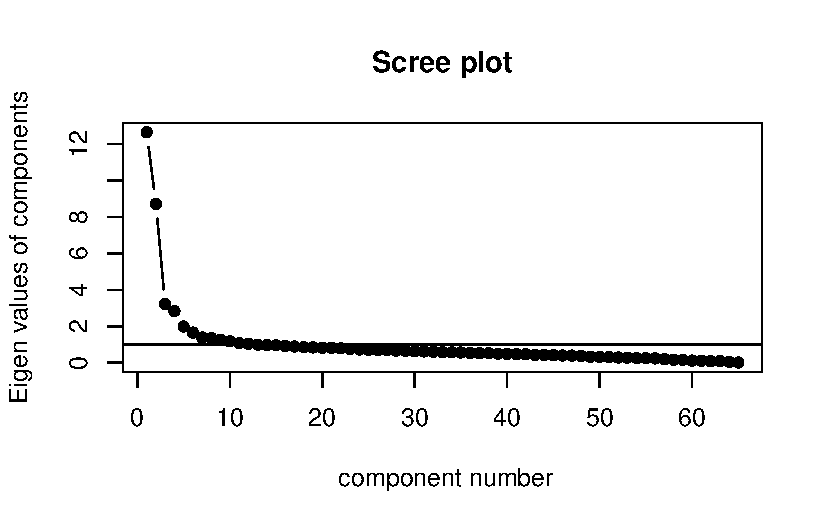
\includegraphics[keepaspectratio]{AppendixF_files/figure-pdf/screeplot-1.pdf}}

\begin{Shaded}
\begin{Highlighting}[]
\CommentTok{\#dev.off()}

\CommentTok{\# Perform PCA}
\NormalTok{pca1 }\OtherTok{\textless{}{-}}\NormalTok{ psych}\SpecialCharTok{::}\FunctionTok{principal}\NormalTok{(TxBdata[,}\DecValTok{7}\SpecialCharTok{:}\FunctionTok{ncol}\NormalTok{(TxBdata)], }
                         \AttributeTok{nfactors =} \DecValTok{6}\NormalTok{,}
                         \AttributeTok{rotate =} \StringTok{"none"}\NormalTok{)}
\CommentTok{\#pca1$loadings}
\end{Highlighting}
\end{Shaded}

\subsection{Excluding features with low final
communalites}\label{excluding-features-with-low-final-communalites}

We first check whether some feature have extremely low communalities
(see
\href{https://rdrr.io/cran/FactorAssumptions/man/communalities_optimal_solution.htmlhttps://rdrr.io/cran/FactorAssumptions/man/communalities_optimal_solution.html}{https://rdrr.io/cran/FactorAssumptions/man/communalities\_optimal\_solution.html}).

\begin{verbatim}
  STPR   MDNE    HDG  CAUSE   FREQ   THRC    POS   PROG    ACT   DEMO   MDWS 
  0.09   0.17   0.17   0.19   0.22   0.22   0.24   0.26   0.26   0.27   0.28 
   CUZ   COND   QUPR  EXIST   MDCO  NCOMP  OCCUR   TIME ASPECT  TPP3P    AMP 
  0.28   0.28   0.29   0.29   0.31   0.31   0.32   0.32   0.33   0.33   0.34 
    RP  THATD   THSC     EX  FPP1P  PLACE    PIT    VBG   PEAS   MDCA  DOAUX 
  0.34   0.36   0.39   0.43   0.43   0.43   0.45   0.46   0.47   0.48   0.48 
   VBN   JJPR   JJAT   WHSC  SPLIT   EMPH   QUAN MENTAL  TPP3S   PASS   YNQU 
  0.48   0.49   0.49   0.50   0.51   0.53   0.55   0.56   0.56   0.57   0.58 
POLITE     RB     CC    XX0     DT   COMM   WHQU    TTR  FPP1S     IN     LD 
  0.58   0.58   0.58   0.59   0.62   0.62   0.64   0.65   0.67   0.68   0.68 
  FPUH   VPRT   SPP2   BEMA    DMA    VBD    AWL   CONT     NN   VIMP 
  0.70   0.71   0.72   0.74   0.74   0.80   0.85   0.85   0.87   0.90 
\end{verbatim}

As we chose to exclude features with communalities of \textless{} 0.2,
we remove STPR, HDG, MDNE and CAUSE from the dataset to be analysed.

\begin{Shaded}
\begin{Highlighting}[]
\NormalTok{TxBdataforPCA }\OtherTok{\textless{}{-}}\NormalTok{ TxBdata }\SpecialCharTok{|\textgreater{}} 
  \FunctionTok{select}\NormalTok{(}\SpecialCharTok{{-}}\FunctionTok{c}\NormalTok{(STPR, MDNE, HDG, CAUSE))}
\end{Highlighting}
\end{Shaded}

The overall MSA value of the dataset is now 0.88. None of the remaining
features have individual MSA values below 0.5:

\begin{Shaded}
\begin{Highlighting}[]
\NormalTok{kmo3}\SpecialCharTok{$}\NormalTok{MSAi[}\FunctionTok{order}\NormalTok{(kmo3}\SpecialCharTok{$}\NormalTok{MSAi)] }\SpecialCharTok{|\textgreater{}}\FunctionTok{round}\NormalTok{(}\DecValTok{2}\NormalTok{)}
\end{Highlighting}
\end{Shaded}

\begin{verbatim}
  MDWS   MDCA    POS   FREQ    VBD  TPP3S   VPRT    ACT     LD   COND     DT 
  0.54   0.64   0.64   0.65   0.65   0.66   0.66   0.67   0.69   0.78   0.79 
  MDCO  TPP3P     RP  NCOMP   VIMP   SPP2  DOAUX MENTAL   WHSC    VBG  THATD 
  0.79   0.81   0.82   0.82   0.82   0.82   0.84   0.85   0.86   0.86   0.86 
 EXIST  FPP1S   COMM     NN     IN   WHQU   DEMO ASPECT   JJAT   THRC     EX 
  0.86   0.87   0.88   0.89   0.89   0.89   0.89   0.89   0.89   0.90   0.90 
 OCCUR   PEAS     CC   YNQU   QUAN    AWL   TIME    XX0  FPP1P    TTR   CONT 
  0.90   0.91   0.91   0.91   0.91   0.92   0.92   0.92   0.92   0.92   0.93 
  PROG   BEMA  SPLIT   PASS   JJPR   THSC     RB   QUPR    AMP   FPUH    PIT 
  0.93   0.93   0.93   0.94   0.94   0.95   0.95   0.95   0.95   0.95   0.95 
   VBN    DMA POLITE    CUZ   EMPH  PLACE 
  0.95   0.96   0.96   0.96   0.96   0.97 
\end{verbatim}

The final number of linguistic features entered in the intra-textbook
model of linguistic variation is 61.

\section{Testing the effect of rotating the
components}\label{testing-the-effect-of-rotating-the-components}

This chunk was used when considering whether or not to rotate the
components (see methods section). Ultimately, the components were not
rotated.

\begin{Shaded}
\begin{Highlighting}[]
\CommentTok{\# Comparing a rotated vs. a non{-}rotated solution}

\CommentTok{\#TxBdata \textless{}{-} readRDS(here("data", "processed", "TxBdataforPCA.rds"))}

\CommentTok{\# No rotation}
\NormalTok{pca2 }\OtherTok{\textless{}{-}}\NormalTok{ psych}\SpecialCharTok{::}\FunctionTok{principal}\NormalTok{(TxBdata[,}\DecValTok{7}\SpecialCharTok{:}\FunctionTok{ncol}\NormalTok{(TxBdata)], }
                         \AttributeTok{nfactors =} \DecValTok{6}\NormalTok{, }
                         \AttributeTok{rotate =} \StringTok{"none"}\NormalTok{)}

\NormalTok{pca2}\SpecialCharTok{$}\NormalTok{loadings}

\FunctionTok{biplot.psych}\NormalTok{(pca2, }
             \AttributeTok{vars =} \ConstantTok{TRUE}\NormalTok{, }
             \AttributeTok{choose=}\FunctionTok{c}\NormalTok{(}\DecValTok{1}\NormalTok{,}\DecValTok{2}\NormalTok{),}
\NormalTok{             )}

\CommentTok{\# Promax rotation}
\NormalTok{pca2.rotated }\OtherTok{\textless{}{-}}\NormalTok{ psych}\SpecialCharTok{::}\FunctionTok{principal}\NormalTok{(TxBdata[,}\DecValTok{7}\SpecialCharTok{:}\FunctionTok{ncol}\NormalTok{(TxBdata)], }
                         \AttributeTok{nfactors =} \DecValTok{6}\NormalTok{, }
                         \AttributeTok{rotate =} \StringTok{"promax"}\NormalTok{)}

\CommentTok{\# This summary shows the component correlations which is particularly interesting}
\NormalTok{pca2.rotated}

\NormalTok{pca2.rotated}\SpecialCharTok{$}\NormalTok{loadings}

\FunctionTok{biplot.psych}\NormalTok{(pca2.rotated, }\AttributeTok{vars =} \ConstantTok{TRUE}\NormalTok{, }\AttributeTok{choose=}\FunctionTok{c}\NormalTok{(}\DecValTok{1}\NormalTok{,}\DecValTok{2}\NormalTok{))}
\end{Highlighting}
\end{Shaded}

\section{Principal Component Analysis
(PCA)}\label{principal-component-analysis-pca}

\subsection{Using the full dataset}\label{using-the-full-dataset}

Except outliers removed as part of the data preparation (see Appendix
D).

\begin{Shaded}
\begin{Highlighting}[]
\CommentTok{\# Perform PCA on full data}
\NormalTok{TxBdata }\OtherTok{\textless{}{-}} \FunctionTok{readRDS}\NormalTok{(}\FunctionTok{here}\NormalTok{(}\StringTok{"data"}\NormalTok{, }\StringTok{"processed"}\NormalTok{, }\StringTok{"TxBdataforPCA.rds"}\NormalTok{))}
\end{Highlighting}
\end{Shaded}

\subsection{Using random subsets of the
data}\label{using-random-subsets-of-the-data}

Alternatively, it is possible to conduct the PCA on random subsets of
the data to test the stability of the solution. Re-running this line
will generate a new subset of the TEC texts containing 2/3 of the texts
randomly sampled.

\begin{Shaded}
\begin{Highlighting}[]
\NormalTok{TxBdata }\OtherTok{\textless{}{-}} \FunctionTok{readRDS}\NormalTok{(}\FunctionTok{here}\NormalTok{(}\StringTok{"data"}\NormalTok{, }\StringTok{"processed"}\NormalTok{, }\StringTok{"TxBdataforPCA.rds"}\NormalTok{)) }\SpecialCharTok{|\textgreater{}}
  \FunctionTok{slice\_sample}\NormalTok{(}\AttributeTok{n =} \FunctionTok{round}\NormalTok{(}\DecValTok{1961}\SpecialCharTok{*}\FloatTok{0.6}\NormalTok{), }\AttributeTok{replace =} \ConstantTok{FALSE}\NormalTok{)}

\FunctionTok{nrow}\NormalTok{(TxBdata)}
\NormalTok{TxBdata}\SpecialCharTok{$}\NormalTok{Filename[}\DecValTok{1}\SpecialCharTok{:}\DecValTok{10}\NormalTok{]}
\FunctionTok{nrow}\NormalTok{(TxBdata) }\SpecialCharTok{/}\NormalTok{ (}\FunctionTok{ncol}\NormalTok{(TxBdata)}\SpecialCharTok{{-}}\DecValTok{6}\NormalTok{) }\CommentTok{\# Check that there is enough data to conduct a PCA. This ratio should be at least 5 (see Friginal \& Hardy 2014: 303–304).}
\end{Highlighting}
\end{Shaded}

\subsection{Using specific subsets of the
data}\label{using-specific-subsets-of-the-data}

The following chunk can be used to perform the PCA on a country subset
of the data to test the stability of the solution. See (Le Foll) for a
detailed analysis of the subcorpus of textbooks used in Germany.

\begin{Shaded}
\begin{Highlighting}[]
\NormalTok{TxBdata }\OtherTok{\textless{}{-}} \FunctionTok{readRDS}\NormalTok{(}\FunctionTok{here}\NormalTok{(}\StringTok{"data"}\NormalTok{, }\StringTok{"processed"}\NormalTok{, }\StringTok{"TxBdataforPCA.rds"}\NormalTok{)) }\SpecialCharTok{|\textgreater{}}
  \CommentTok{\#filter(Country == "France")}
  \CommentTok{\#filter(Country == "Germany")}
  \FunctionTok{filter}\NormalTok{(Country }\SpecialCharTok{==} \StringTok{"Spain"}\NormalTok{)}

\FunctionTok{nrow}\NormalTok{(TxBdata)}
\NormalTok{TxBdata}\SpecialCharTok{$}\NormalTok{Filename[}\DecValTok{1}\SpecialCharTok{:}\DecValTok{10}\NormalTok{] }\CommentTok{\# Check data}
\FunctionTok{nrow}\NormalTok{(TxBdata) }\SpecialCharTok{/}\NormalTok{ (}\FunctionTok{ncol}\NormalTok{(TxBdata)}\SpecialCharTok{{-}}\DecValTok{6}\NormalTok{) }\CommentTok{\# Check that there is enough data to conduct a PCA. This should be \textgreater{} 5 (see Friginal \& Hardy 2014: 303–304).}
\end{Highlighting}
\end{Shaded}

\subsection{Performing the PCA}\label{performing-the-pca}

We perform the PCA using the \texttt{prcomp} function and print a
summary of the results.

\begin{Shaded}
\begin{Highlighting}[]
\NormalTok{pca }\OtherTok{\textless{}{-}} \FunctionTok{prcomp}\NormalTok{(TxBdata[,}\DecValTok{7}\SpecialCharTok{:}\FunctionTok{ncol}\NormalTok{(TxBdata)], }\AttributeTok{scale.=}\ConstantTok{FALSE}\NormalTok{, }\AttributeTok{rank. =} \DecValTok{6}\NormalTok{) }\CommentTok{\# All quantitative variables for all TxB files except outliers}
\NormalTok{register  }\OtherTok{\textless{}{-}} \FunctionTok{factor}\NormalTok{(TxBdata[,}\StringTok{"Register"}\NormalTok{]) }\CommentTok{\# Register}
\NormalTok{level }\OtherTok{\textless{}{-}} \FunctionTok{factor}\NormalTok{(TxBdata[,}\StringTok{"Level"}\NormalTok{]) }\CommentTok{\# Textbook proficiency level}

\CommentTok{\# summary(register)}
\CommentTok{\# summary(level)}
\FunctionTok{summary}\NormalTok{(pca)}
\end{Highlighting}
\end{Shaded}

\begin{verbatim}
Importance of first k=6 (out of 61) components:
                          PC1    PC2     PC3     PC4     PC5     PC6
Standard deviation     2.1693 1.7776 1.08902 1.00207 0.84288 0.76792
Proportion of Variance 0.2108 0.1416 0.05313 0.04499 0.03183 0.02642
Cumulative Proportion  0.2108 0.3524 0.40553 0.45051 0.48234 0.50876
\end{verbatim}

\section{Plotting PCA results}\label{plotting-pca-results}

\subsection{3D plots}\label{d-plots}

The following chunk can be used to create projections of TEC texts on
three dimensions of the model. These plots cannot be rendered in two
dimensions and are therefore not generated in the present document. For
more information on the \texttt{pca3d} library, see:
\url{https://cran.r-project.org/web/packages/pca3d/vignettes/pca3d.pdf}.

\begin{Shaded}
\begin{Highlighting}[]
\FunctionTok{library}\NormalTok{(pca3d) }\CommentTok{\# For 3{-}D plots}

\NormalTok{col }\OtherTok{\textless{}{-}}\NormalTok{ palette[}\FunctionTok{c}\NormalTok{(}\DecValTok{1}\SpecialCharTok{:}\DecValTok{3}\NormalTok{,}\DecValTok{8}\NormalTok{,}\DecValTok{7}\NormalTok{)] }\CommentTok{\# without poetry}
\FunctionTok{names}\NormalTok{(col) }\OtherTok{\textless{}{-}} \FunctionTok{c}\NormalTok{(}\StringTok{"Conversation"}\NormalTok{, }\StringTok{"Fiction"}\NormalTok{, }\StringTok{"Informative"}\NormalTok{, }\StringTok{"Instructional"}\NormalTok{, }\StringTok{"Personal"}\NormalTok{)}
\NormalTok{scales}\SpecialCharTok{::}\FunctionTok{show\_col}\NormalTok{(col) }\CommentTok{\# Check colours}

\FunctionTok{pca3d}\NormalTok{(pca, }
      \AttributeTok{group =}\NormalTok{ register,}
      \AttributeTok{components =} \DecValTok{1}\SpecialCharTok{:}\DecValTok{3}\NormalTok{,}
      \CommentTok{\#components = 4:6,}
      \AttributeTok{show.ellipses=}\ConstantTok{FALSE}\NormalTok{, }
      \AttributeTok{ellipse.ci=}\FloatTok{0.75}\NormalTok{,}
      \AttributeTok{show.plane=}\ConstantTok{FALSE}\NormalTok{,}
      \AttributeTok{col =}\NormalTok{ col,}
      \AttributeTok{shape =} \StringTok{"sphere"}\NormalTok{,}
      \AttributeTok{radius =} \DecValTok{1}\NormalTok{,}
      \AttributeTok{legend =} \StringTok{"right"}\NormalTok{)}

\FunctionTok{snapshotPCA3d}\NormalTok{(}\FunctionTok{here}\NormalTok{(}\StringTok{"plots"}\NormalTok{, }\StringTok{"PCA\_TxB\_3Dsnapshot.png"}\NormalTok{))}

\FunctionTok{names}\NormalTok{(col) }\OtherTok{\textless{}{-}} \FunctionTok{c}\NormalTok{(}\StringTok{"C"}\NormalTok{, }\StringTok{"B"}\NormalTok{, }\StringTok{"E"}\NormalTok{, }\StringTok{"A"}\NormalTok{, }\StringTok{"D"}\NormalTok{) }\CommentTok{\# To colour the dots according to the profiency level of the textbooks}
\FunctionTok{pca3d}\NormalTok{(pca, }
      \AttributeTok{components =} \DecValTok{4}\SpecialCharTok{:}\DecValTok{6}\NormalTok{,}
      \AttributeTok{group =}\NormalTok{ level,}
      \AttributeTok{show.ellipses=}\ConstantTok{FALSE}\NormalTok{, }
      \AttributeTok{ellipse.ci=}\FloatTok{0.75}\NormalTok{,}
      \AttributeTok{show.plane=}\ConstantTok{FALSE}\NormalTok{,}
      \AttributeTok{col =}\NormalTok{ col,}
      \AttributeTok{shape =} \StringTok{"sphere"}\NormalTok{,}
      \AttributeTok{radius =} \FloatTok{0.8}\NormalTok{,}
      \AttributeTok{legend =} \StringTok{"right"}\NormalTok{)}
\end{Highlighting}
\end{Shaded}

\section{Two-dimensional plots
(biplots)}\label{two-dimensional-plots-biplots}

These plots were generated using the \texttt{PCAtools} package, which
requires the data to be formatted in a rather unconventional way so it
needs to wrangled first.

\subsection{Data wrangling for
PCAtools}\label{data-wrangling-for-pcatools}

\begin{Shaded}
\begin{Highlighting}[]
\CommentTok{\#TxBdata \textless{}{-} readRDS(here("data", "processed", "TxBdataforPCA.rds"))}

\NormalTok{TxBdata2meta }\OtherTok{\textless{}{-}}\NormalTok{ TxBdata[,}\DecValTok{1}\SpecialCharTok{:}\DecValTok{6}\NormalTok{]}
\FunctionTok{rownames}\NormalTok{(TxBdata2meta) }\OtherTok{\textless{}{-}}\NormalTok{ TxBdata2meta}\SpecialCharTok{$}\NormalTok{Filename}
\NormalTok{TxBdata2meta }\OtherTok{\textless{}{-}}\NormalTok{ TxBdata2meta }\SpecialCharTok{|\textgreater{}} \FunctionTok{select}\NormalTok{(}\SpecialCharTok{{-}}\NormalTok{Filename)}
\CommentTok{\#head(TxBdata2meta)}

\NormalTok{TxBdata2 }\OtherTok{=}\NormalTok{ TxBdata}
\FunctionTok{rownames}\NormalTok{(TxBdata2) }\OtherTok{\textless{}{-}}\NormalTok{ TxBdata2}\SpecialCharTok{$}\NormalTok{Filename}
\NormalTok{TxBdata2num }\OtherTok{\textless{}{-}} \FunctionTok{as.data.frame}\NormalTok{(base}\SpecialCharTok{::}\FunctionTok{t}\NormalTok{(TxBdata2[,}\DecValTok{7}\SpecialCharTok{:}\FunctionTok{ncol}\NormalTok{(TxBdata2)]))}
\CommentTok{\#TxBdata2num[1:12,1:3] \# Check sanity of data}

\NormalTok{p }\OtherTok{\textless{}{-}}\NormalTok{ PCAtools}\SpecialCharTok{::}\FunctionTok{pca}\NormalTok{(TxBdata2num, }
         \AttributeTok{metadata =}\NormalTok{ TxBdata2meta,}
         \AttributeTok{scale =} \ConstantTok{FALSE}\NormalTok{)}
\end{Highlighting}
\end{Shaded}

\subsection{Pairs plot}\label{pairs-plot}

We first produce a scatterplot matrix of all the combinations of the
first six dimensions of the model of intra-textbook variation. Note that
the number before the comma on each axis label shows which principal
component is plotted on that axis; this is followed by the percentage of
the total variance explained by that particular component. The colours
correspond to the text registers.

\begin{Shaded}
\begin{Highlighting}[]
\DocumentationTok{\#\# Colour and shape scheme for all biplots}
\NormalTok{colkey }\OtherTok{=} \FunctionTok{c}\NormalTok{(}\AttributeTok{Conversation=}\StringTok{"\#BD241E"}\NormalTok{, }\AttributeTok{Fiction=}\StringTok{"\#A18A33"}\NormalTok{, }\AttributeTok{Informative=}\StringTok{"\#15274D"}\NormalTok{, }\AttributeTok{Instructional=}\StringTok{"\#F9B921"}\NormalTok{, }\AttributeTok{Personal=}\StringTok{"\#722672"}\NormalTok{)}
\NormalTok{shapekey }\OtherTok{=} \FunctionTok{c}\NormalTok{(}\AttributeTok{A=}\DecValTok{1}\NormalTok{, }\AttributeTok{B=}\DecValTok{2}\NormalTok{, }\AttributeTok{C=}\DecValTok{6}\NormalTok{, }\AttributeTok{D=}\DecValTok{0}\NormalTok{, }\AttributeTok{E=}\DecValTok{5}\NormalTok{)}

\DocumentationTok{\#\# Very slow, open in zoomed out window!}
\CommentTok{\# Add legend manually? Yes (take it from the biplot code below), sadly really the simplest solution, here. Or use Evert\textquotesingle{}s mvar.pairs plot function (though that also requires manual axis annotation).}

\CommentTok{\# png(here("plots", "PCA\_TxB\_pairsplot.png"), width = 12, height= 19, units = "cm", res = 300)}
\NormalTok{PCAtools}\SpecialCharTok{::}\FunctionTok{pairsplot}\NormalTok{(p,}
                 \AttributeTok{triangle =} \ConstantTok{FALSE}\NormalTok{,}
                 \AttributeTok{components =} \DecValTok{1}\SpecialCharTok{:}\DecValTok{6}\NormalTok{,}
                 \AttributeTok{ncol =} \DecValTok{3}\NormalTok{,}
                 \AttributeTok{nrow =} \DecValTok{5}\NormalTok{,}
                 \AttributeTok{pointSize =} \FloatTok{0.8}\NormalTok{,}
                 \AttributeTok{lab =} \ConstantTok{NULL}\NormalTok{, }\CommentTok{\# Otherwise will try to label each data point!}
                 \AttributeTok{colby =} \StringTok{"Register"}\NormalTok{,}
                 \AttributeTok{colkey =}\NormalTok{ colkey,}
                 \AttributeTok{shape =} \StringTok{"Level"}\NormalTok{,}
                 \AttributeTok{shapekey =}\NormalTok{ shapekey,}
                 \AttributeTok{margingaps =} \FunctionTok{unit}\NormalTok{(}\FunctionTok{c}\NormalTok{(}\FloatTok{0.2}\NormalTok{, }\FloatTok{0.2}\NormalTok{, }\FloatTok{0.2}\NormalTok{, }\FloatTok{0.2}\NormalTok{), }\StringTok{"cm"}\NormalTok{),}
                 \AttributeTok{legendPosition =} \StringTok{"none"}\NormalTok{)}
\end{Highlighting}
\end{Shaded}

\pandocbounded{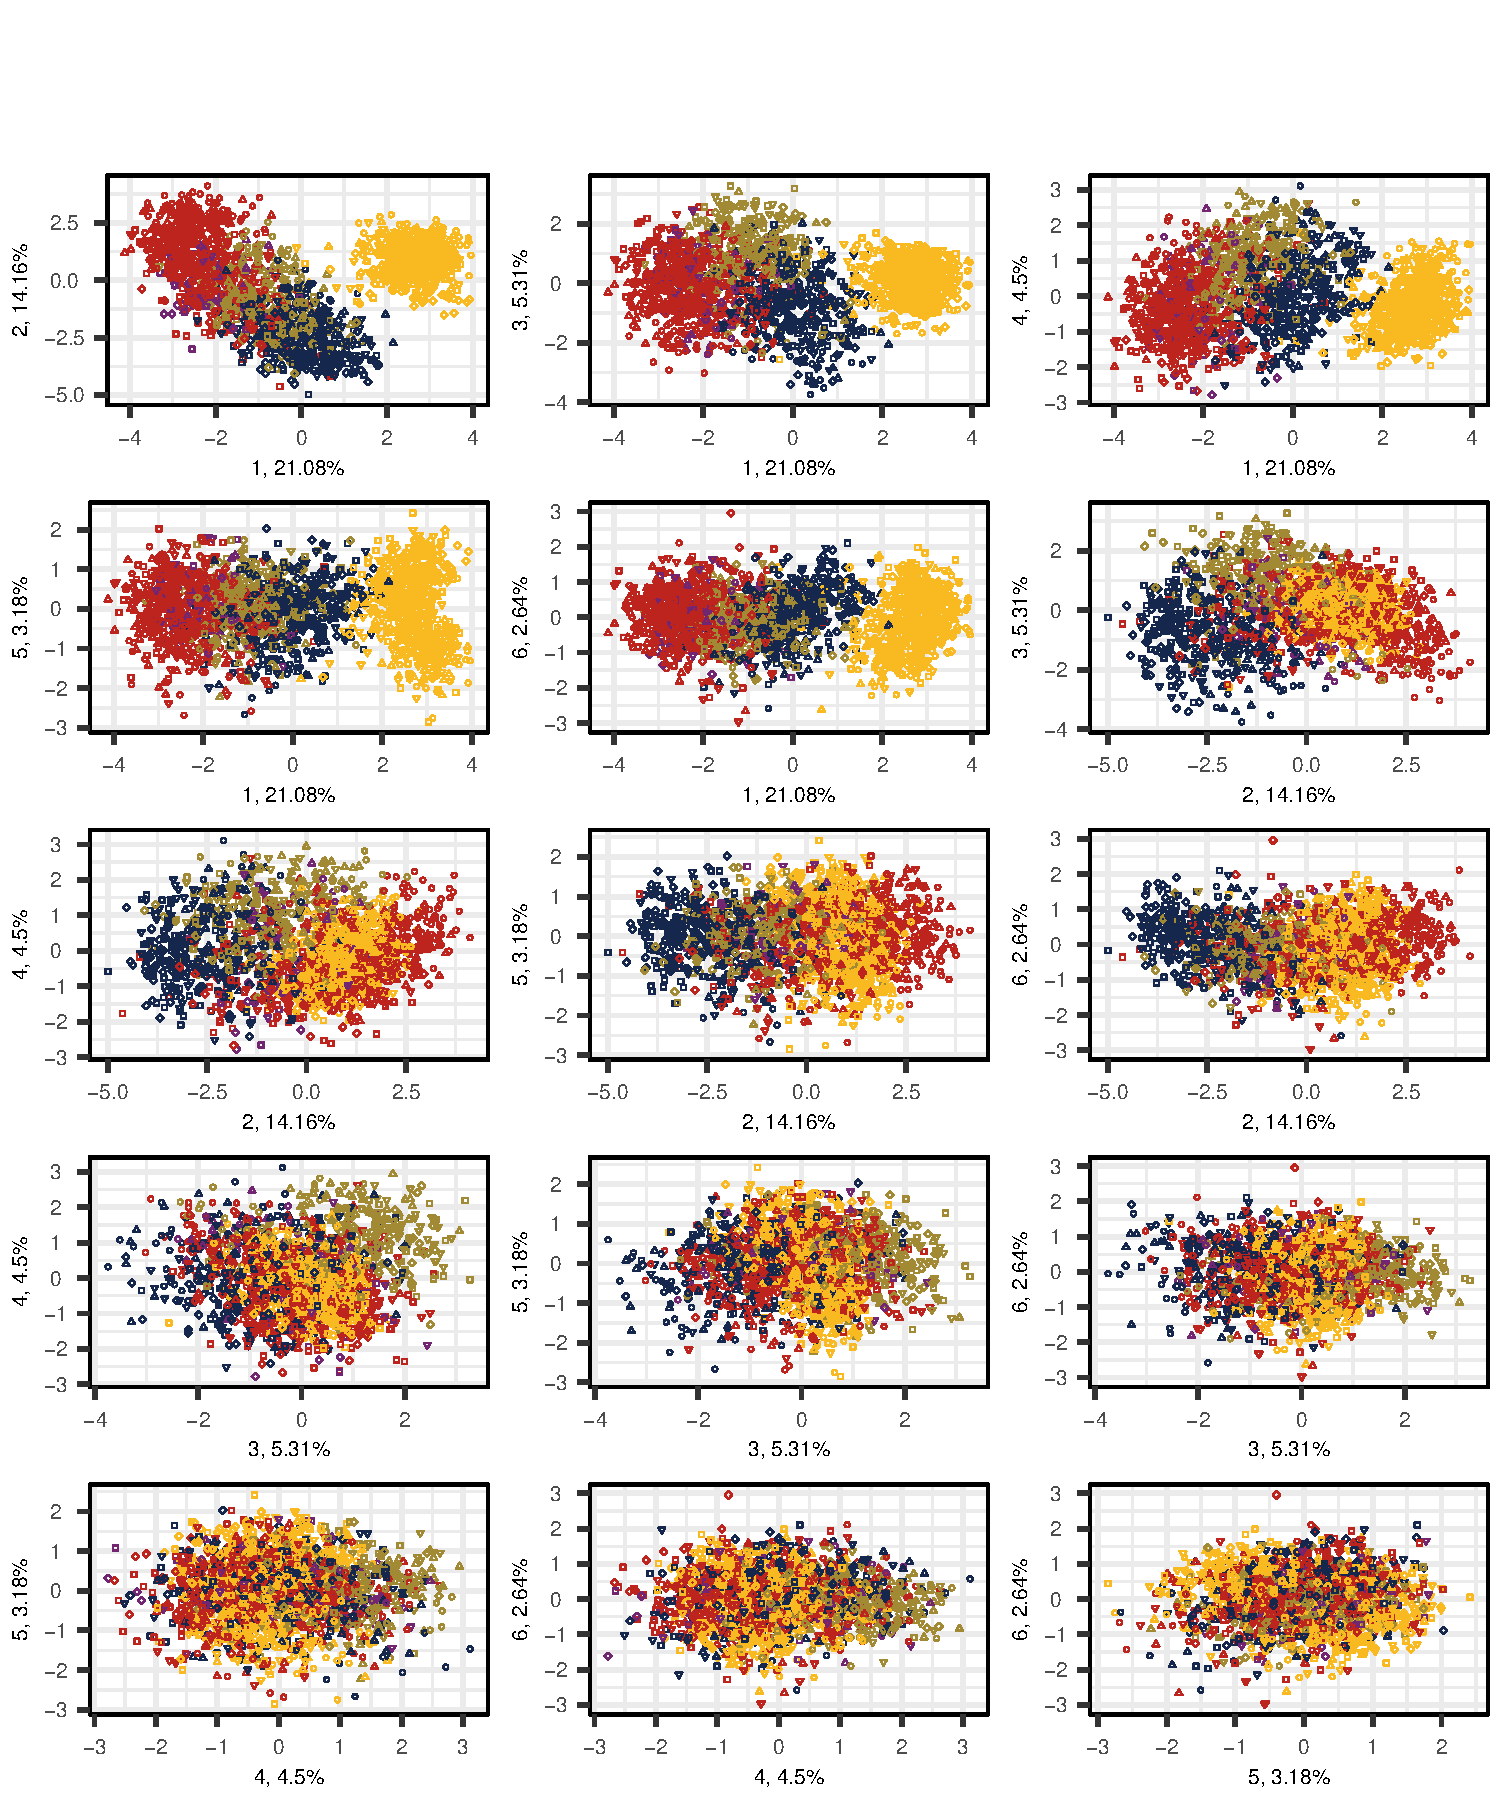
\includegraphics[keepaspectratio]{AppendixF_files/figure-pdf/PCAtools-pairsplots-TxB-1.pdf}}

\subsection{Bi-plots}\label{bi-plots}

Then, biplots of the most important dimensions are generated to examine
components more carefully.

The following biplot displays the distribution of the texts of the TEC
along the first and second dimensions of the intra-textbook model.

\begin{Shaded}
\begin{Highlighting}[]
\NormalTok{colkey }\OtherTok{=} \FunctionTok{c}\NormalTok{(}\AttributeTok{Conversation=}\StringTok{"\#BD241E"}\NormalTok{, }\AttributeTok{Fiction=}\StringTok{"\#A18A33"}\NormalTok{, }\AttributeTok{Informative=}\StringTok{"\#15274D"}\NormalTok{, }\AttributeTok{Instructional=}\StringTok{"\#F9B921"}\NormalTok{, }\AttributeTok{Personal=}\StringTok{"\#722672"}\NormalTok{)}
\NormalTok{shapekey }\OtherTok{=} \FunctionTok{c}\NormalTok{(}\AttributeTok{A=}\DecValTok{1}\NormalTok{, }\AttributeTok{B=}\DecValTok{2}\NormalTok{, }\AttributeTok{C=}\DecValTok{6}\NormalTok{, }\AttributeTok{D=}\DecValTok{0}\NormalTok{, }\AttributeTok{E=}\DecValTok{5}\NormalTok{)}

\CommentTok{\#png(here("plots", "PCA\_TxB\_Biplot\_PC1\_PC2.png"), width = 40, height= 25, units = "cm", res = 300)}
\NormalTok{PCAtools}\SpecialCharTok{::}\FunctionTok{biplot}\NormalTok{(p,}
                 \AttributeTok{x =} \StringTok{"PC1"}\NormalTok{,}
                 \AttributeTok{y =} \StringTok{"PC2"}\NormalTok{,}
                 \AttributeTok{lab =} \ConstantTok{NULL}\NormalTok{, }\CommentTok{\# Otherwise will try to label each data point!}
                 \CommentTok{\#xlim = c(min(p$rotated$PC1){-}0.5, max(p$rotated$PC1)+0.5),}
                 \CommentTok{\#ylim = c(min(p$rotated$PC2){-}0.5, max(p$rotated$PC2)+0.5),}
                 \AttributeTok{colby =} \StringTok{"Register"}\NormalTok{,}
                 \AttributeTok{pointSize =} \DecValTok{2}\NormalTok{,}
                 \AttributeTok{colkey =}\NormalTok{ colkey,}
                 \AttributeTok{shape =} \StringTok{"Level"}\NormalTok{,}
                 \AttributeTok{shapekey =}\NormalTok{ shapekey,}
                 \AttributeTok{showLoadings =} \ConstantTok{FALSE}\NormalTok{,}
                 \AttributeTok{ellipse =} \ConstantTok{TRUE}\NormalTok{,}
                 \AttributeTok{axisLabSize =} \DecValTok{22}\NormalTok{,}
                 \AttributeTok{legendPosition =} \StringTok{\textquotesingle{}right\textquotesingle{}}\NormalTok{,}
                 \AttributeTok{legendTitleSize =} \DecValTok{22}\NormalTok{,}
                 \AttributeTok{legendLabSize =} \DecValTok{18}\NormalTok{, }
                 \AttributeTok{legendIconSize =} \DecValTok{7}\NormalTok{) }\SpecialCharTok{+}
  \FunctionTok{theme}\NormalTok{(}\AttributeTok{plot.margin =} \FunctionTok{unit}\NormalTok{(}\FunctionTok{c}\NormalTok{(}\DecValTok{0}\NormalTok{,}\DecValTok{0}\NormalTok{,}\DecValTok{0}\NormalTok{,}\FloatTok{0.2}\NormalTok{), }\StringTok{"cm"}\NormalTok{))}
\end{Highlighting}
\end{Shaded}

\pandocbounded{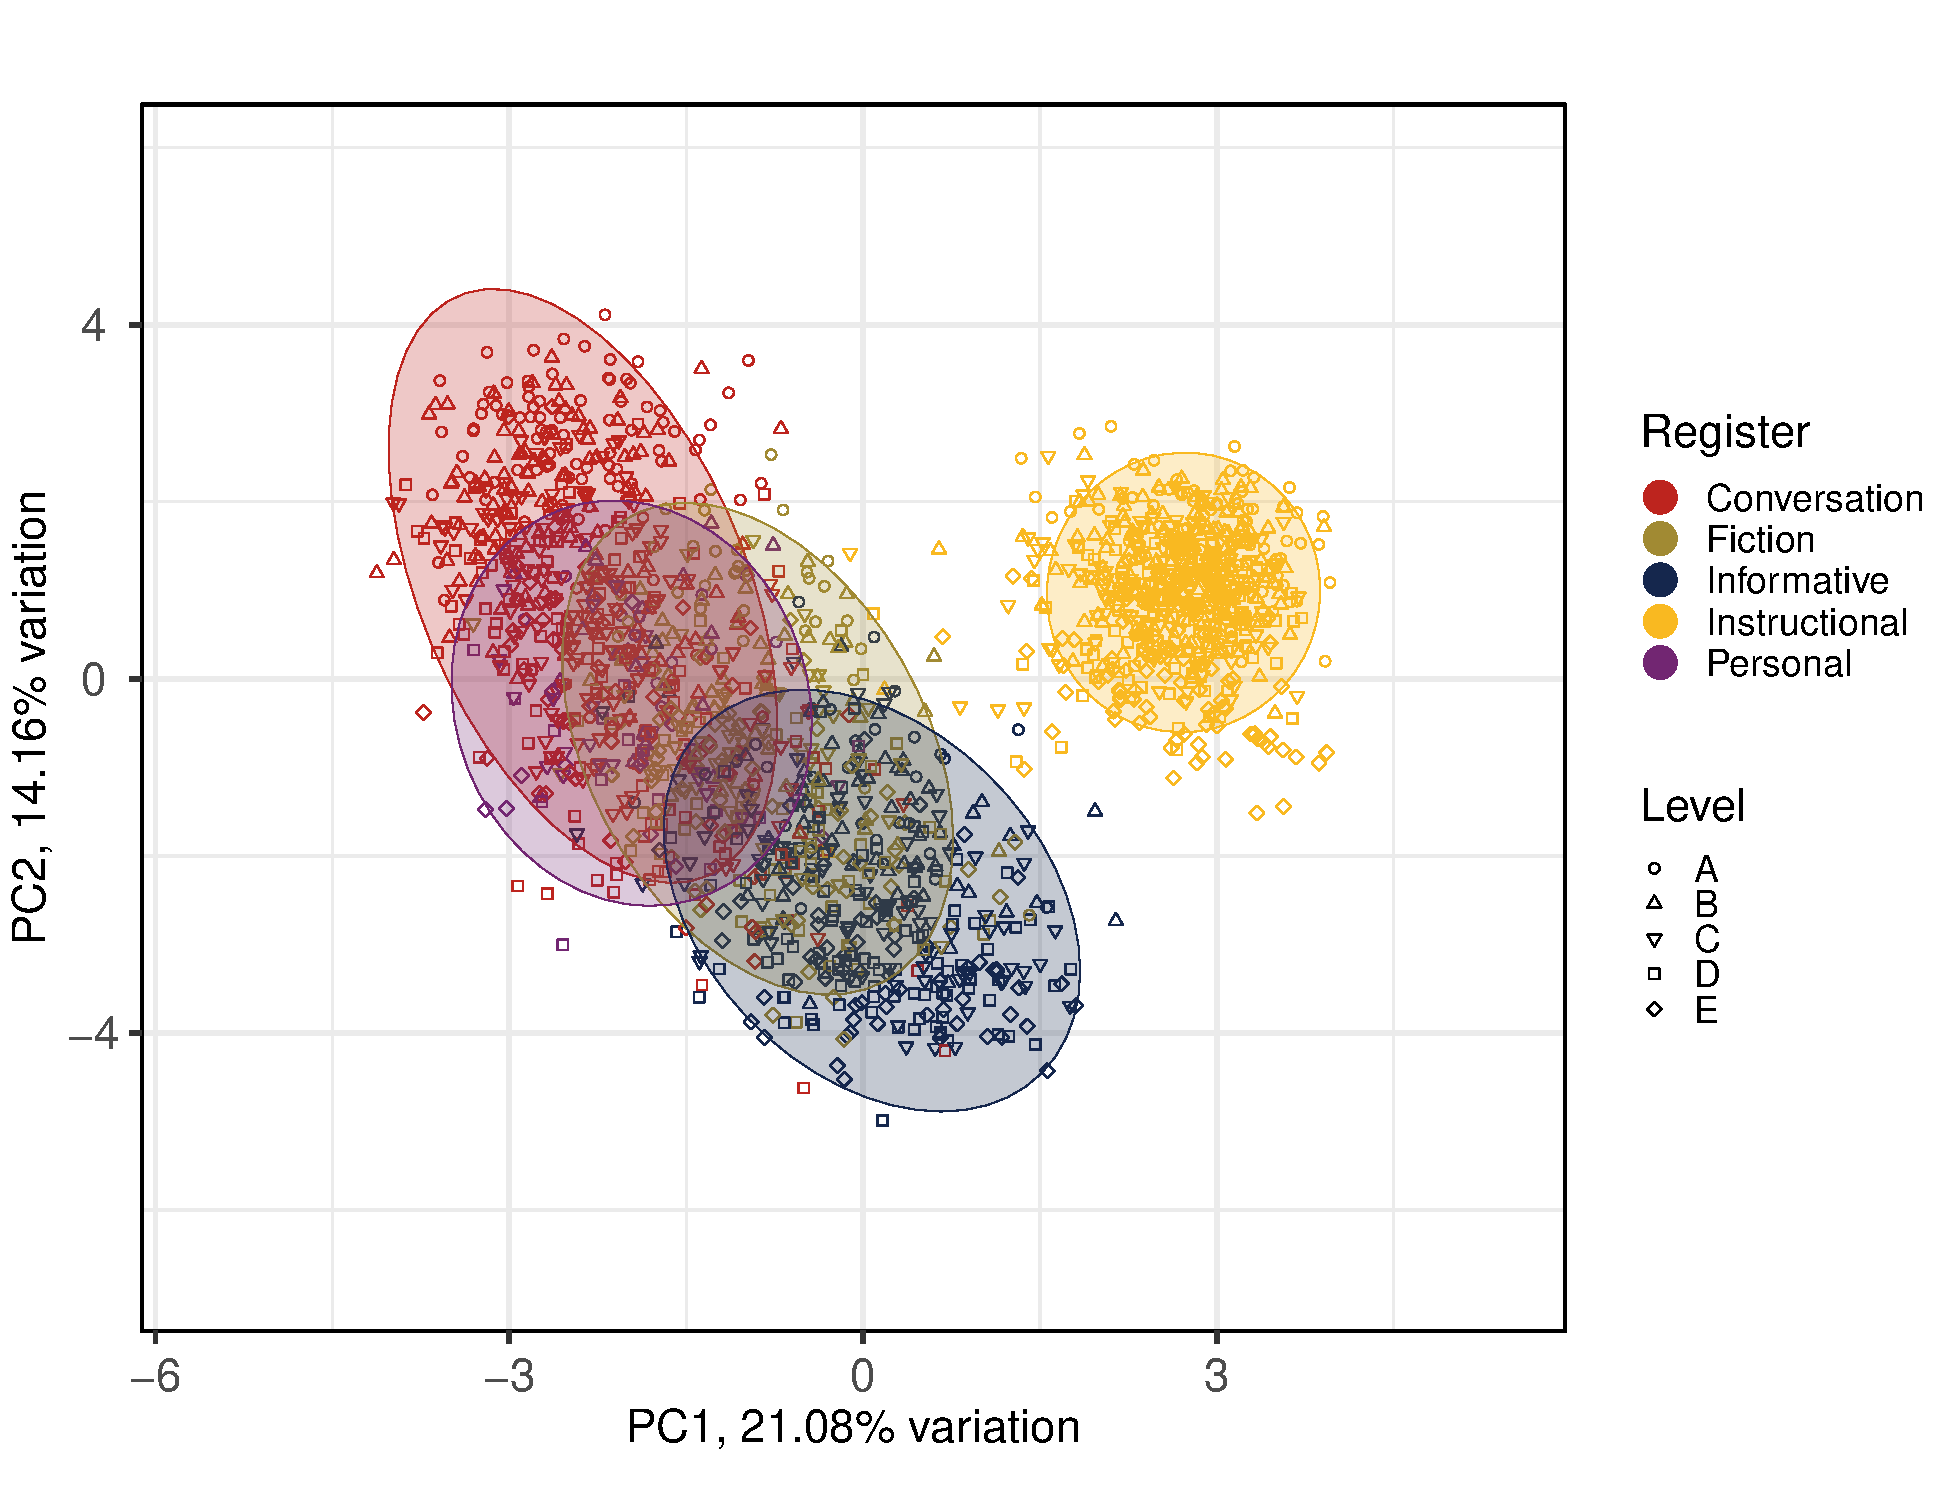
\includegraphics[keepaspectratio]{AppendixF_files/figure-pdf/PCAtools-biplots-TxB-1.pdf}}

\begin{Shaded}
\begin{Highlighting}[]
\CommentTok{\#dev.off()}
\CommentTok{\#ggsave(here("plots", "PCA\_TxB\_BiplotPC1\_PC2.svg"), width = 12, height = 10)}
\end{Highlighting}
\end{Shaded}

The following code chunk can be used for the interactive examination of
individual data points (i.e., texts).

\begin{Shaded}
\begin{Highlighting}[]
\FunctionTok{library}\NormalTok{(plotly)}

\NormalTok{plot }\OtherTok{\textless{}{-}}\NormalTok{ PCAtools}\SpecialCharTok{::}\FunctionTok{biplot}\NormalTok{(p,}
                 \AttributeTok{x =} \StringTok{"PC1"}\NormalTok{,}
                 \AttributeTok{y =} \StringTok{"PC2"}\NormalTok{,}
                 \AttributeTok{lab =} \ConstantTok{NULL}\NormalTok{, }\CommentTok{\# Otherwise will try to label each data point!}
                 \AttributeTok{colby =} \StringTok{"Register"}\NormalTok{,}
                 \AttributeTok{pointSize =} \DecValTok{2}\NormalTok{,}
                 \AttributeTok{colkey =}\NormalTok{ colkey,}
                 \AttributeTok{shape =} \StringTok{"Level"}\NormalTok{,}
                 \AttributeTok{shapekey =}\NormalTok{ shapekey,}
                 \AttributeTok{showLoadings =} \ConstantTok{FALSE}\NormalTok{,}
                 \AttributeTok{ellipse =} \ConstantTok{TRUE}\NormalTok{,}
                 \AttributeTok{axisLabSize =} \DecValTok{22}\NormalTok{,}
                 \AttributeTok{legendPosition =} \StringTok{\textquotesingle{}right\textquotesingle{}}\NormalTok{,}
                 \AttributeTok{legendTitleSize =} \DecValTok{22}\NormalTok{,}
                 \AttributeTok{legendLabSize =} \DecValTok{18}\NormalTok{, }
                 \AttributeTok{legendIconSize =} \DecValTok{7}\NormalTok{) }\SpecialCharTok{+}
  \FunctionTok{theme}\NormalTok{(}\AttributeTok{plot.margin =} \FunctionTok{unit}\NormalTok{(}\FunctionTok{c}\NormalTok{(}\DecValTok{0}\NormalTok{,}\DecValTok{0}\NormalTok{,}\DecValTok{0}\NormalTok{,}\FloatTok{0.2}\NormalTok{), }\StringTok{"cm"}\NormalTok{))}

\FunctionTok{ggplotly}\NormalTok{(plot) }\CommentTok{\# tooltip}

\DocumentationTok{\#\#\#}
\end{Highlighting}
\end{Shaded}

For the fourth to sixth dimensions of the model, it is worth comparing
the effet of text register with that of textbook proficiency level.
Hence, the following two chunks generate biplots with colour and
ellipses representing a) text register (as above) and b) textbook level
(A = first year of EFL tuition at secondary school, E = fifth year).

\begin{Shaded}
\begin{Highlighting}[]
\NormalTok{pRegisters }\OtherTok{\textless{}{-}}\NormalTok{ PCAtools}\SpecialCharTok{::}\FunctionTok{biplot}\NormalTok{(p,}
                 \AttributeTok{x =} \StringTok{"PC3"}\NormalTok{,}
                 \AttributeTok{y =} \StringTok{"PC4"}\NormalTok{,}
                 \AttributeTok{lab =} \ConstantTok{NULL}\NormalTok{, }\CommentTok{\# Otherwise will try to label each data point!}
                 \AttributeTok{colby =} \StringTok{"Register"}\NormalTok{,}
                 \AttributeTok{pointSize =} \DecValTok{2}\NormalTok{,}
                 \AttributeTok{colkey =}\NormalTok{ colkey,}
                 \AttributeTok{shape =} \StringTok{"Level"}\NormalTok{,}
                 \AttributeTok{shapekey =}\NormalTok{ shapekey,}
                 \AttributeTok{showLoadings =} \ConstantTok{FALSE}\NormalTok{,}
                 \AttributeTok{ellipse =} \ConstantTok{TRUE}\NormalTok{,}
                 \AttributeTok{legendPosition =} \StringTok{\textquotesingle{}right\textquotesingle{}}\NormalTok{,}
                 \AttributeTok{legendTitleSize =} \DecValTok{22}\NormalTok{,}
                 \AttributeTok{legendLabSize =} \DecValTok{18}\NormalTok{, }
                 \AttributeTok{legendIconSize =} \DecValTok{7}\NormalTok{) }\SpecialCharTok{+}
  \FunctionTok{theme}\NormalTok{(}\AttributeTok{plot.margin =} \FunctionTok{unit}\NormalTok{(}\FunctionTok{c}\NormalTok{(}\DecValTok{0}\NormalTok{,}\DecValTok{0}\NormalTok{,}\DecValTok{0}\NormalTok{,}\FloatTok{0.2}\NormalTok{), }\StringTok{"cm"}\NormalTok{))}

\CommentTok{\#ggsave(here("plots", "PCA\_TxB\_BiplotPC3\_PC4.svg"), width = 12, height = 10)}

\NormalTok{pRegisters2 }\OtherTok{\textless{}{-}}\NormalTok{ PCAtools}\SpecialCharTok{::}\FunctionTok{biplot}\NormalTok{(p,}
                 \AttributeTok{x =} \StringTok{"PC5"}\NormalTok{,}
                 \AttributeTok{y =} \StringTok{"PC6"}\NormalTok{,}
                 \AttributeTok{lab =} \ConstantTok{NULL}\NormalTok{, }\CommentTok{\# Otherwise will try to label each data point!}
                 \AttributeTok{colby =} \StringTok{"Register"}\NormalTok{,}
                 \AttributeTok{pointSize =} \DecValTok{2}\NormalTok{,}
                 \AttributeTok{colkey =}\NormalTok{ colkey,}
                 \AttributeTok{shape =} \StringTok{"Level"}\NormalTok{,}
                 \AttributeTok{shapekey =}\NormalTok{ shapekey,}
                 \AttributeTok{showLoadings =} \ConstantTok{FALSE}\NormalTok{,}
                 \AttributeTok{ellipse =} \ConstantTok{TRUE}\NormalTok{,}
                 \AttributeTok{legendPosition =} \StringTok{\textquotesingle{}right\textquotesingle{}}\NormalTok{,}
                 \AttributeTok{legendTitleSize =} \DecValTok{22}\NormalTok{,}
                 \AttributeTok{legendLabSize =} \DecValTok{18}\NormalTok{, }
                 \AttributeTok{legendIconSize =} \DecValTok{7}\NormalTok{) }\SpecialCharTok{+}
  \FunctionTok{theme}\NormalTok{(}\AttributeTok{plot.margin =} \FunctionTok{unit}\NormalTok{(}\FunctionTok{c}\NormalTok{(}\DecValTok{0}\NormalTok{,}\DecValTok{0}\NormalTok{,}\DecValTok{0}\NormalTok{,}\FloatTok{0.2}\NormalTok{), }\StringTok{"cm"}\NormalTok{))}

\CommentTok{\#ggsave(here("plots", "PCA\_TxB\_BiplotPC5\_PC6.svg"), width = 12, height = 10)}
\end{Highlighting}
\end{Shaded}

\begin{Shaded}
\begin{Highlighting}[]
\CommentTok{\# Inverted keys for the biplots with ellipses for Level rather than Register}
\NormalTok{colkeyLevels }\OtherTok{=} \FunctionTok{c}\NormalTok{(}\AttributeTok{A=}\StringTok{"\#F9B921"}\NormalTok{, }\AttributeTok{B=}\StringTok{"\#A18A33"}\NormalTok{, }\AttributeTok{C=}\StringTok{"\#BD241E"}\NormalTok{, }\AttributeTok{D=}\StringTok{"\#722672"}\NormalTok{, }\AttributeTok{E=}\StringTok{"\#15274D"}\NormalTok{)}
\NormalTok{shapekeyLevels }\OtherTok{=} \FunctionTok{c}\NormalTok{(}\AttributeTok{Conversation=}\DecValTok{1}\NormalTok{, }\AttributeTok{Fiction=}\DecValTok{2}\NormalTok{, }\AttributeTok{Informative=}\DecValTok{6}\NormalTok{, }\AttributeTok{Instructional=}\DecValTok{0}\NormalTok{, }\AttributeTok{Personal=}\DecValTok{5}\NormalTok{)}

\NormalTok{pLevels }\OtherTok{\textless{}{-}}\NormalTok{ PCAtools}\SpecialCharTok{::}\FunctionTok{biplot}\NormalTok{(p,}
                 \AttributeTok{x =} \StringTok{"PC3"}\NormalTok{,}
                 \AttributeTok{y =} \StringTok{"PC4"}\NormalTok{,}
                 \AttributeTok{lab =} \ConstantTok{NULL}\NormalTok{, }\CommentTok{\# Otherwise will try to label each data point!}
                 \CommentTok{\#xlim = c(min(p$rotated$PC1){-}0.5, max(p$rotated$PC1)+0.5),}
                 \CommentTok{\#ylim = c(min(p$rotated$PC2){-}0.5, max(p$rotated$PC2)+0.5),}
                 \AttributeTok{colby =} \StringTok{"Level"}\NormalTok{,}
                 \AttributeTok{pointSize =} \DecValTok{2}\NormalTok{,}
                 \AttributeTok{colkey =}\NormalTok{ colkeyLevels,}
                 \AttributeTok{shape =} \StringTok{"Register"}\NormalTok{,}
                 \AttributeTok{shapekey =}\NormalTok{ shapekeyLevels,}
                 \AttributeTok{showLoadings =} \ConstantTok{FALSE}\NormalTok{,}
                 \AttributeTok{ellipse =} \ConstantTok{TRUE}\NormalTok{,}
                 \AttributeTok{legendPosition =} \StringTok{\textquotesingle{}right\textquotesingle{}}\NormalTok{,}
                 \AttributeTok{legendTitleSize =} \DecValTok{22}\NormalTok{,}
                 \AttributeTok{legendLabSize =} \DecValTok{18}\NormalTok{, }
                 \AttributeTok{legendIconSize =} \DecValTok{7}\NormalTok{) }\SpecialCharTok{+}
  \FunctionTok{theme}\NormalTok{(}\AttributeTok{plot.margin =} \FunctionTok{unit}\NormalTok{(}\FunctionTok{c}\NormalTok{(}\DecValTok{0}\NormalTok{,}\DecValTok{0}\NormalTok{,}\DecValTok{0}\NormalTok{,}\FloatTok{0.2}\NormalTok{), }\StringTok{"cm"}\NormalTok{))}
\CommentTok{\#ggsave(here("plots", "PCA\_TxB\_BiplotPC3\_PC4\_Level.svg"), width = 12, height = 10)}

\NormalTok{pLevels2 }\OtherTok{\textless{}{-}}\NormalTok{ PCAtools}\SpecialCharTok{::}\FunctionTok{biplot}\NormalTok{(p,}
                 \AttributeTok{x =} \StringTok{"PC5"}\NormalTok{,}
                 \AttributeTok{y =} \StringTok{"PC6"}\NormalTok{,}
                 \AttributeTok{lab =} \ConstantTok{NULL}\NormalTok{, }\CommentTok{\# Otherwise will try to label each data point!}
                 \CommentTok{\#xlim = c(min(p$rotated$PC1){-}0.5, max(p$rotated$PC1)+0.5),}
                 \CommentTok{\#ylim = c(min(p$rotated$PC2){-}0.5, max(p$rotated$PC2)+0.5),}
                 \AttributeTok{colby =} \StringTok{"Level"}\NormalTok{,}
                 \AttributeTok{pointSize =} \DecValTok{2}\NormalTok{,}
                 \AttributeTok{colkey =}\NormalTok{ colkeyLevels,}
                 \AttributeTok{shape =} \StringTok{"Register"}\NormalTok{,}
                 \AttributeTok{shapekey =}\NormalTok{ shapekeyLevels,}
                 \AttributeTok{showLoadings =} \ConstantTok{FALSE}\NormalTok{,}
                 \AttributeTok{ellipse =} \ConstantTok{TRUE}\NormalTok{,}
                 \AttributeTok{legendPosition =} \StringTok{\textquotesingle{}right\textquotesingle{}}\NormalTok{,}
                 \AttributeTok{legendTitleSize =} \DecValTok{22}\NormalTok{,}
                 \AttributeTok{legendLabSize =} \DecValTok{18}\NormalTok{, }
                 \AttributeTok{legendIconSize =} \DecValTok{7}\NormalTok{) }\SpecialCharTok{+}
  \FunctionTok{theme}\NormalTok{(}\AttributeTok{plot.margin =} \FunctionTok{unit}\NormalTok{(}\FunctionTok{c}\NormalTok{(}\DecValTok{0}\NormalTok{,}\DecValTok{0}\NormalTok{,}\DecValTok{0}\NormalTok{,}\FloatTok{0.2}\NormalTok{), }\StringTok{"cm"}\NormalTok{))}
\CommentTok{\#ggsave(here("plots", "PCA\_TxB\_BiplotPC5\_PC6\_Level.svg"), width = 12, height = 10)}
\end{Highlighting}
\end{Shaded}

The following biplots display the distribution of the texts of the TEC
along the third and fourth dimensions of the intra-textbook model.

\pandocbounded{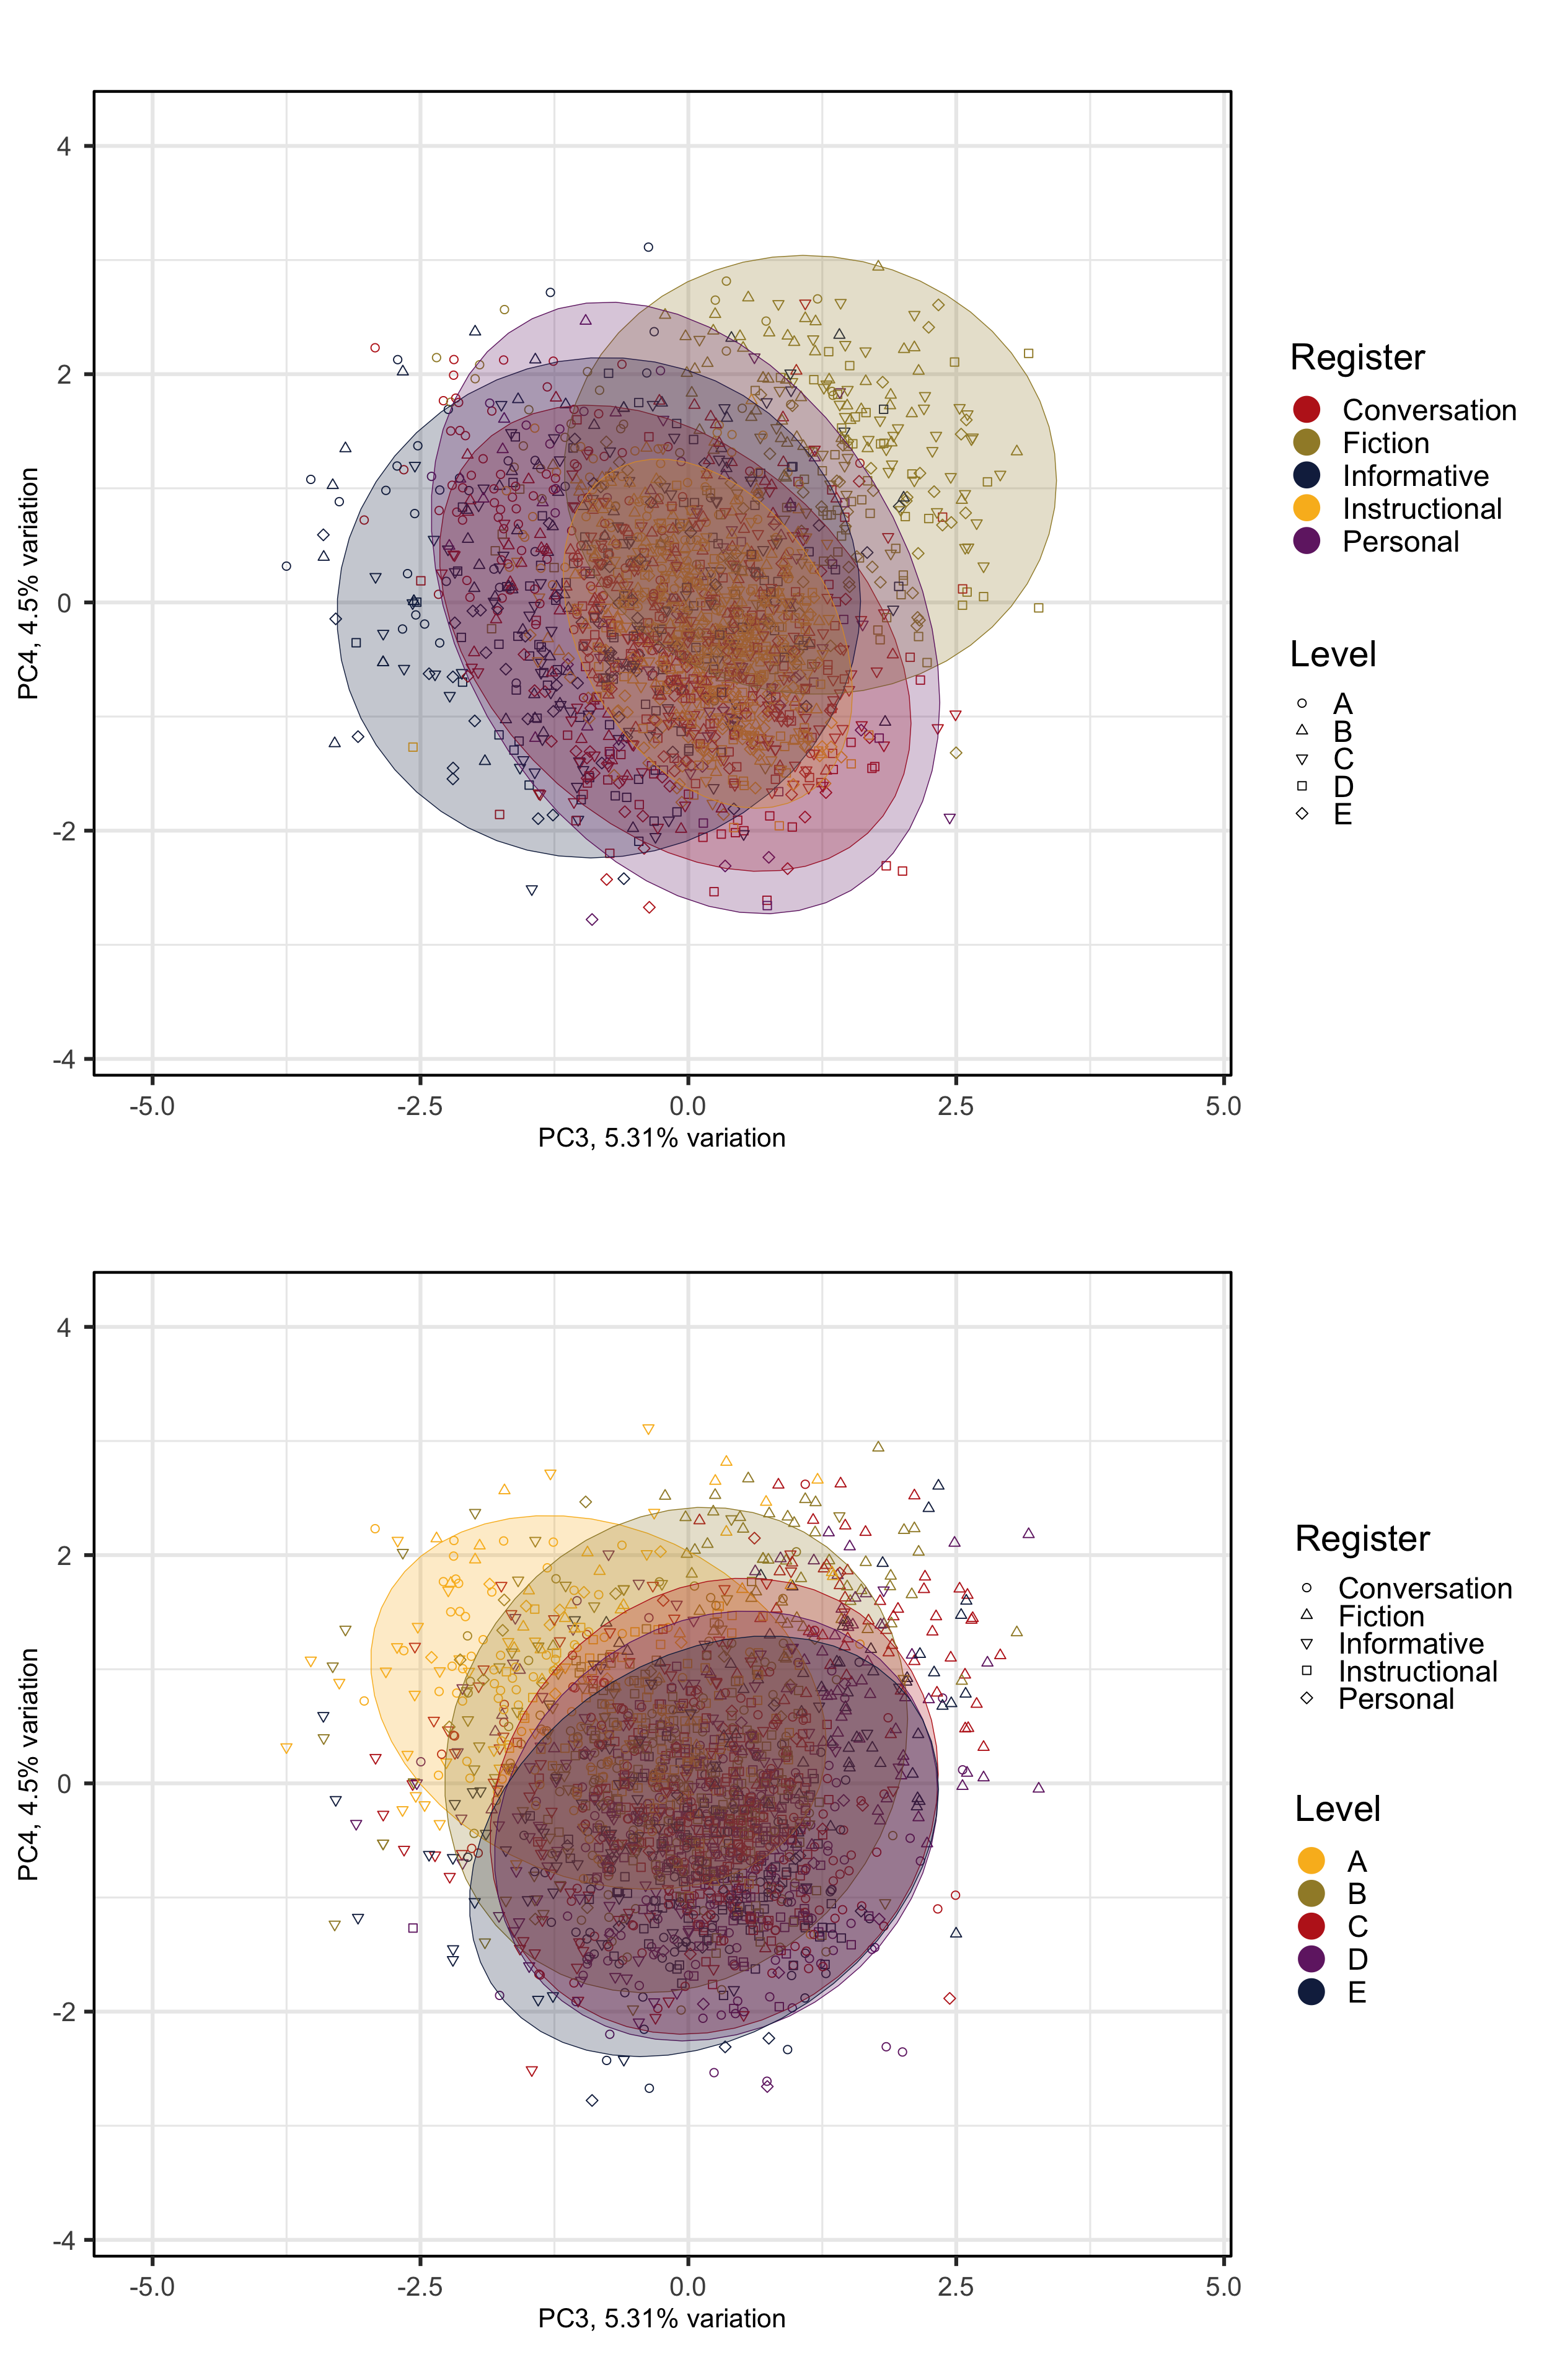
\includegraphics[keepaspectratio]{AppendixF_files/figure-pdf/PCAtools-biplots-TxB-PC3-4-1.pdf}}

The following biplots display the distribution of the texts of the TEC
along the fifth and sixth dimensions of the intra-textbook model.

\pandocbounded{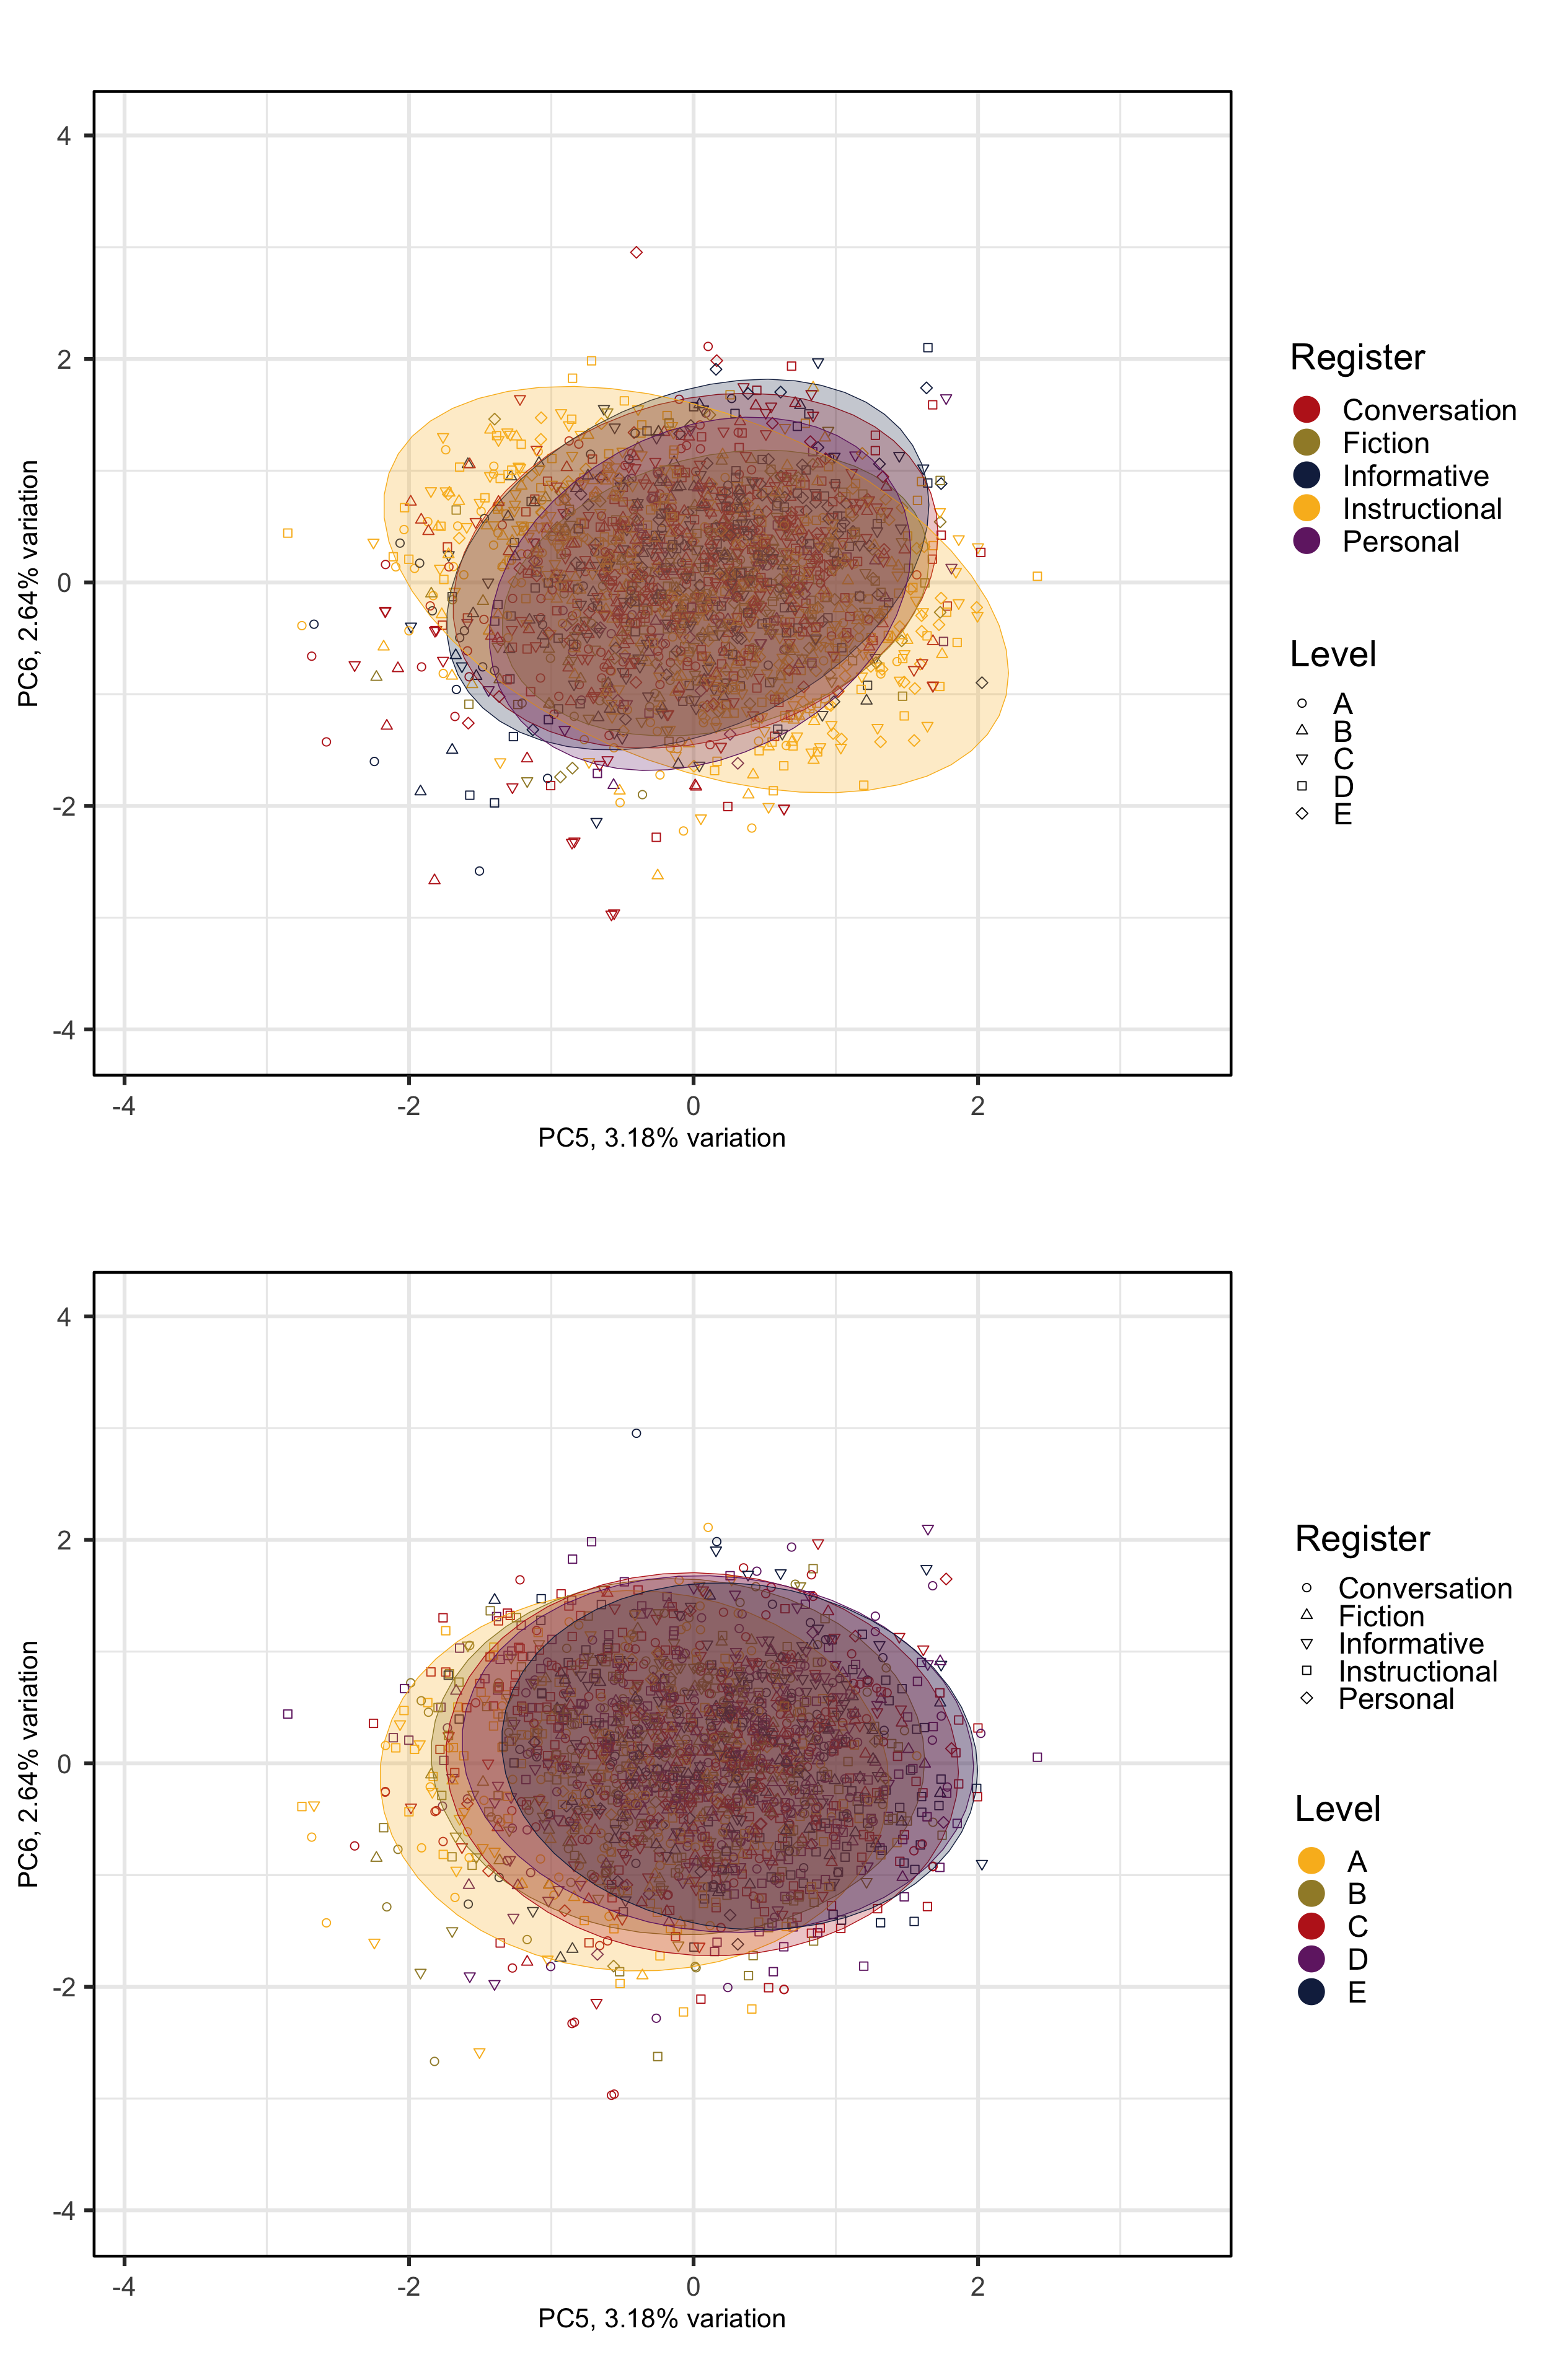
\includegraphics[keepaspectratio]{AppendixF_files/figure-pdf/PCAtools-biplots-TxB-PC5-6-1.pdf}}

\section{Feature contributions (loadings) on each
component}\label{feature-contributions-loadings-on-each-component}

\begin{Shaded}
\begin{Highlighting}[]
\CommentTok{\#TxBdata \textless{}{-} readRDS(here("data", "processed", "TxBdataforPCA.rds"))}

\NormalTok{pca }\OtherTok{\textless{}{-}} \FunctionTok{prcomp}\NormalTok{(TxBdata[,}\DecValTok{7}\SpecialCharTok{:}\FunctionTok{ncol}\NormalTok{(TxBdata)], }\AttributeTok{scale.=}\ConstantTok{FALSE}\NormalTok{) }\CommentTok{\# All quantitative variables for all TEC files}

\CommentTok{\# The rotated data that represents the observations / samples is stored in rotated, while the variable loadings are stored in loadings}
\NormalTok{loadings }\OtherTok{\textless{}{-}} \FunctionTok{as.data.frame}\NormalTok{(pca}\SpecialCharTok{$}\NormalTok{rotation[,}\DecValTok{1}\SpecialCharTok{:}\DecValTok{4}\NormalTok{])}
\NormalTok{loadings }\SpecialCharTok{|\textgreater{}} 
  \FunctionTok{round}\NormalTok{(}\DecValTok{2}\NormalTok{) }\SpecialCharTok{|\textgreater{}} 
  \FunctionTok{kable}\NormalTok{()}
\end{Highlighting}
\end{Shaded}

\begin{longtable}[]{@{}lrrrr@{}}
\toprule\noalign{}
& PC1 & PC2 & PC3 & PC4 \\
\midrule\noalign{}
\endhead
\bottomrule\noalign{}
\endlastfoot
ACT & 0.08 & -0.11 & 0.04 & -0.10 \\
AMP & -0.12 & -0.10 & -0.11 & 0.01 \\
ASPECT & 0.10 & -0.05 & 0.14 & -0.01 \\
AWL & 0.22 & -0.16 & -0.12 & -0.13 \\
BEMA & -0.22 & 0.01 & -0.21 & 0.02 \\
CC & 0.05 & -0.21 & -0.19 & 0.00 \\
COMM & 0.20 & 0.09 & 0.14 & -0.04 \\
COND & -0.01 & -0.02 & 0.11 & -0.24 \\
CONT & -0.25 & 0.11 & -0.03 & -0.06 \\
CUZ & -0.09 & -0.13 & -0.06 & -0.02 \\
DEMO & -0.12 & 0.08 & 0.03 & -0.09 \\
DMA & -0.20 & 0.14 & -0.02 & 0.00 \\
DOAUX & -0.01 & 0.20 & 0.05 & -0.15 \\
DT & 0.12 & 0.00 & 0.31 & -0.02 \\
EMPH & -0.19 & -0.02 & 0.06 & -0.14 \\
EX & -0.10 & -0.05 & -0.11 & 0.05 \\
EXIST & -0.02 & -0.15 & -0.09 & -0.09 \\
FPP1P & -0.17 & 0.01 & -0.07 & 0.00 \\
FPP1S & -0.23 & 0.07 & 0.08 & -0.01 \\
FPUH & -0.16 & 0.15 & -0.09 & 0.07 \\
FREQ & -0.03 & -0.05 & 0.01 & -0.10 \\
IN & 0.17 & -0.18 & 0.02 & -0.08 \\
JJAT & -0.06 & -0.18 & 0.04 & -0.21 \\
JJPR & -0.17 & -0.06 & -0.11 & -0.11 \\
LD & 0.16 & -0.03 & -0.26 & -0.01 \\
MDCA & -0.04 & 0.10 & -0.18 & -0.09 \\
MDCO & -0.05 & -0.10 & 0.22 & 0.01 \\
MDWS & -0.07 & -0.01 & 0.05 & -0.16 \\
MENTAL & 0.14 & 0.13 & 0.12 & -0.25 \\
NCOMP & 0.04 & -0.05 & -0.24 & -0.15 \\
NN & 0.20 & -0.09 & -0.29 & 0.11 \\
OCCUR & 0.02 & -0.18 & 0.03 & 0.02 \\
PASS & -0.01 & -0.22 & -0.06 & -0.05 \\
PEAS & -0.06 & -0.17 & 0.13 & -0.13 \\
PIT & -0.19 & -0.04 & -0.06 & -0.06 \\
PLACE & -0.16 & -0.01 & -0.07 & 0.09 \\
POLITE & -0.14 & 0.13 & -0.07 & 0.02 \\
POS & -0.01 & 0.03 & -0.04 & 0.16 \\
PROG & -0.11 & -0.02 & 0.11 & 0.00 \\
QUAN & -0.15 & -0.03 & 0.12 & -0.19 \\
QUPR & -0.10 & -0.05 & 0.16 & -0.11 \\
RB & -0.19 & -0.08 & 0.20 & 0.00 \\
RP & 0.00 & -0.09 & 0.14 & 0.02 \\
SPLIT & -0.11 & -0.18 & 0.02 & -0.16 \\
SPP2 & 0.10 & 0.22 & -0.01 & -0.25 \\
THATD & -0.05 & 0.04 & 0.16 & -0.24 \\
THRC & 0.02 & -0.11 & -0.02 & -0.18 \\
THSC & -0.06 & -0.17 & 0.07 & -0.14 \\
TIME & -0.12 & -0.08 & -0.01 & 0.06 \\
TPP3P & -0.01 & -0.16 & -0.09 & -0.02 \\
TPP3S & -0.06 & -0.11 & 0.13 & 0.30 \\
TTR & -0.04 & -0.26 & -0.05 & -0.01 \\
VBD & -0.08 & -0.20 & 0.23 & 0.30 \\
VBG & 0.04 & -0.18 & 0.00 & -0.22 \\
VBN & 0.03 & -0.18 & -0.07 & -0.04 \\
VIMP & 0.25 & 0.15 & 0.04 & -0.08 \\
VPRT & -0.15 & 0.05 & -0.32 & -0.22 \\
WHQU & 0.11 & 0.23 & 0.00 & -0.09 \\
WHSC & 0.11 & -0.11 & 0.03 & -0.15 \\
XX0 & -0.22 & 0.03 & 0.06 & -0.06 \\
YNQU & -0.03 & 0.23 & 0.00 & -0.08 \\
\end{longtable}

We can go back to the normalised frequencies of the individual features
to compare them across different registers and levels, e.g.:

\begin{Shaded}
\begin{Highlighting}[]
\NormalTok{TxBcounts }\SpecialCharTok{|\textgreater{}} 
  \FunctionTok{group\_by}\NormalTok{(Register, Level) }\SpecialCharTok{|\textgreater{}} 
  \FunctionTok{summarise}\NormalTok{(}\FunctionTok{median}\NormalTok{(NCOMP), }\FunctionTok{MAD}\NormalTok{(NCOMP)) }\SpecialCharTok{|\textgreater{}} 
  \FunctionTok{select}\NormalTok{(}\DecValTok{1}\SpecialCharTok{:}\DecValTok{4}\NormalTok{) }\SpecialCharTok{|\textgreater{}} 
  \FunctionTok{kable}\NormalTok{(}\AttributeTok{digits=}\DecValTok{2}\NormalTok{)}
\end{Highlighting}
\end{Shaded}

\begin{longtable}[]{@{}llrr@{}}
\toprule\noalign{}
Register & Level & median(NCOMP) & MAD(NCOMP) \\
\midrule\noalign{}
\endhead
\bottomrule\noalign{}
\endlastfoot
Conversation & A & 5.69 & 2.79 \\
Conversation & B & 5.48 & 2.66 \\
Conversation & C & 5.32 & 2.58 \\
Conversation & D & 6.18 & 2.91 \\
Conversation & E & 6.21 & 2.62 \\
Fiction & A & 4.14 & 2.34 \\
Fiction & B & 3.96 & 2.17 \\
Fiction & C & 4.05 & 1.86 \\
Fiction & D & 5.05 & 2.34 \\
Fiction & E & 5.05 & 2.16 \\
Informative & A & 8.07 & 2.48 \\
Informative & B & 7.62 & 2.40 \\
Informative & C & 7.49 & 3.16 \\
Informative & D & 7.56 & 2.46 \\
Informative & E & 8.77 & 2.45 \\
Instructional & A & 6.84 & 2.54 \\
Instructional & B & 6.80 & 2.65 \\
Instructional & C & 6.14 & 2.35 \\
Instructional & D & 6.22 & 2.29 \\
Instructional & E & 6.75 & 2.69 \\
Personal & A & 6.72 & 1.42 \\
Personal & B & 4.92 & 2.33 \\
Personal & C & 5.75 & 1.45 \\
Personal & D & 6.46 & 3.19 \\
Personal & E & 8.22 & 3.09 \\
\end{longtable}

Graphs of features display the features with the strongest contributions
to any two dimensions of the model of intra-textbook variation. They are
created using the \texttt{factoextra::fviz\_pca\_var} function.

\begin{Shaded}
\begin{Highlighting}[]
\NormalTok{factoextra}\SpecialCharTok{::}\FunctionTok{fviz\_pca\_var}\NormalTok{(pca,}
             \AttributeTok{axes =} \FunctionTok{c}\NormalTok{(}\DecValTok{1}\NormalTok{,}\DecValTok{2}\NormalTok{),}
             \AttributeTok{select.var =} \FunctionTok{list}\NormalTok{(}\AttributeTok{cos2 =} \FloatTok{0.1}\NormalTok{),}
             \AttributeTok{col.var =} \StringTok{"contrib"}\NormalTok{, }\CommentTok{\# Colour by contributions to the PC}
             \AttributeTok{gradient.cols =} \FunctionTok{c}\NormalTok{(}\StringTok{"\#F9B921"}\NormalTok{, }\StringTok{"\#DB241E"}\NormalTok{, }\StringTok{"\#722672"}\NormalTok{),}
             \AttributeTok{title =} \StringTok{""}\NormalTok{,}
             \AttributeTok{repel =} \ConstantTok{TRUE}\NormalTok{, }\CommentTok{\# Try to avoid too much text overlapping}
             \AttributeTok{ggtheme =}\NormalTok{ ggthemes}\SpecialCharTok{::}\FunctionTok{theme\_few}\NormalTok{())}
\end{Highlighting}
\end{Shaded}

\pandocbounded{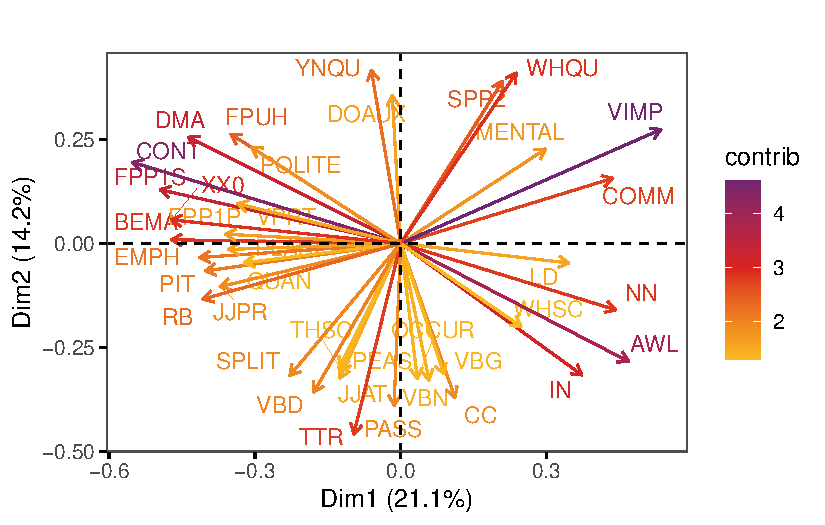
\includegraphics[keepaspectratio]{AppendixF_files/figure-pdf/graphs-of-variables-1.pdf}}

\begin{Shaded}
\begin{Highlighting}[]
\CommentTok{\#ggsave(here("plots", "fviz\_pca\_var\_PC1\_PC2.svg"), width = 11, height = 9)}

\NormalTok{factoextra}\SpecialCharTok{::}\FunctionTok{fviz\_pca\_var}\NormalTok{(pca,}
             \AttributeTok{axes =} \FunctionTok{c}\NormalTok{(}\DecValTok{3}\NormalTok{,}\DecValTok{2}\NormalTok{),}
             \AttributeTok{select.var =} \FunctionTok{list}\NormalTok{(}\AttributeTok{contrib =} \DecValTok{30}\NormalTok{),}
             \AttributeTok{col.var =} \StringTok{"contrib"}\NormalTok{, }\CommentTok{\# Colour by contributions to the PC}
             \AttributeTok{gradient.cols =} \FunctionTok{c}\NormalTok{(}\StringTok{"\#F9B921"}\NormalTok{, }\StringTok{"\#DB241E"}\NormalTok{, }\StringTok{"\#722672"}\NormalTok{),}
             \AttributeTok{title =} \StringTok{""}\NormalTok{,}
             \AttributeTok{repel =} \ConstantTok{TRUE}\NormalTok{, }\CommentTok{\# Try to avoid too much text overlapping}
             \AttributeTok{ggtheme =}\NormalTok{ ggthemes}\SpecialCharTok{::}\FunctionTok{theme\_few}\NormalTok{())}
\end{Highlighting}
\end{Shaded}

\pandocbounded{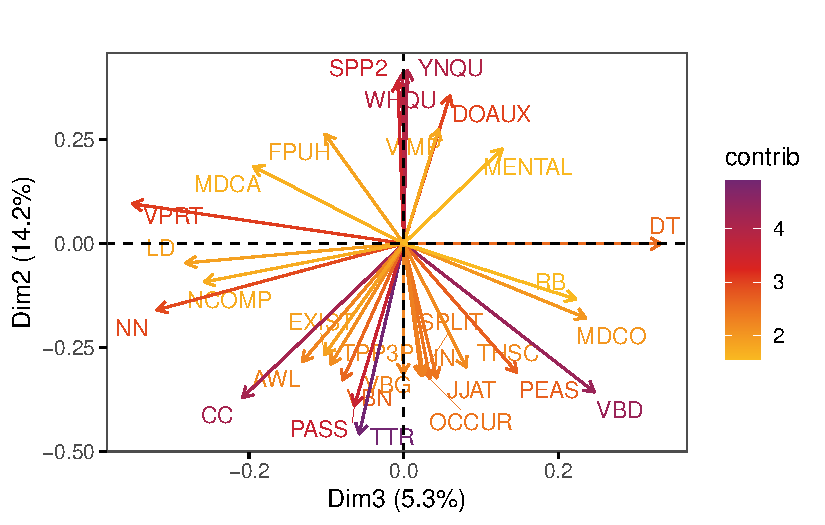
\includegraphics[keepaspectratio]{AppendixF_files/figure-pdf/graphs-of-variables-2.pdf}}

\begin{Shaded}
\begin{Highlighting}[]
\CommentTok{\#ggsave(here("plots", "fviz\_pca\_var\_PC3\_PC2.svg"), width = 9, height = 8)}

\NormalTok{factoextra}\SpecialCharTok{::}\FunctionTok{fviz\_pca\_var}\NormalTok{(pca,}
             \AttributeTok{axes =} \FunctionTok{c}\NormalTok{(}\DecValTok{3}\NormalTok{,}\DecValTok{4}\NormalTok{),}
             \AttributeTok{select.var =} \FunctionTok{list}\NormalTok{(}\AttributeTok{contrib =} \DecValTok{30}\NormalTok{),}
             \AttributeTok{col.var =} \StringTok{"contrib"}\NormalTok{, }\CommentTok{\# Colour by contributions to the PC}
             \AttributeTok{gradient.cols =} \FunctionTok{c}\NormalTok{(}\StringTok{"\#F9B921"}\NormalTok{, }\StringTok{"\#DB241E"}\NormalTok{, }\StringTok{"\#722672"}\NormalTok{),}
             \AttributeTok{title =} \StringTok{""}\NormalTok{,}
             \AttributeTok{repel =} \ConstantTok{TRUE}\NormalTok{, }\CommentTok{\# Try to avoid too much text overlapping}
             \AttributeTok{ggtheme =}\NormalTok{ ggthemes}\SpecialCharTok{::}\FunctionTok{theme\_few}\NormalTok{())}
\end{Highlighting}
\end{Shaded}

\pandocbounded{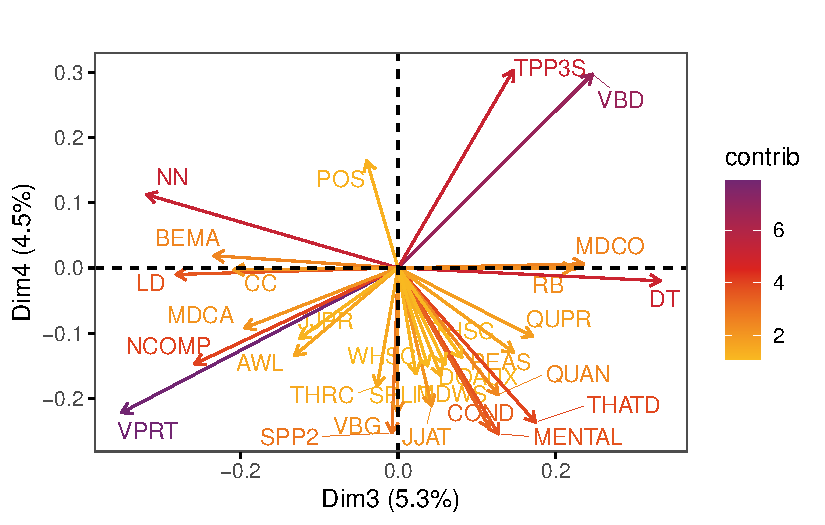
\includegraphics[keepaspectratio]{AppendixF_files/figure-pdf/graphs-of-variables-3.pdf}}

\begin{Shaded}
\begin{Highlighting}[]
\CommentTok{\#ggsave(here("plots", "fviz\_pca\_var\_PC3\_PC4.svg"), width = 9, height = 8)}
\end{Highlighting}
\end{Shaded}

\section{Exploring the dimensions of the
model}\label{exploring-the-dimensions-of-the-model}

We begin with some descriptive statistics of the dimension scores.

\begin{Shaded}
\begin{Highlighting}[]
\CommentTok{\# http://www.sthda.com/english/articles/31{-}principal{-}component{-}methods{-}in{-}r{-}practical{-}guide/118{-}principal{-}component{-}analysis{-}in{-}r{-}prcomp{-}vs{-}princomp/\#pca{-}results{-}for{-}variables}

\CommentTok{\#TxBdata \textless{}{-} readRDS(here("data", "processed", "TxBdataforPCA.rds"))}

\NormalTok{pca }\OtherTok{\textless{}{-}} \FunctionTok{prcomp}\NormalTok{(TxBdata[,}\DecValTok{7}\SpecialCharTok{:}\FunctionTok{ncol}\NormalTok{(TxBdata)], }\AttributeTok{scale.=}\ConstantTok{FALSE}\NormalTok{) }\CommentTok{\# All quantitative variables for all TxB files}
\NormalTok{register  }\OtherTok{\textless{}{-}} \FunctionTok{factor}\NormalTok{(TxBdata[,}\StringTok{"Register"}\NormalTok{]) }\CommentTok{\# Register}
\NormalTok{level }\OtherTok{\textless{}{-}} \FunctionTok{factor}\NormalTok{(TxBdata[,}\StringTok{"Level"}\NormalTok{]) }\CommentTok{\# Textbook proficiency level}

\CommentTok{\# summary(register)}
\CommentTok{\# summary(level)}
\CommentTok{\# summary(pca)}

\DocumentationTok{\#\# Access to the PCA results for individual PC}
\CommentTok{\#pca$rotation[,1]}

\NormalTok{res.ind }\OtherTok{\textless{}{-}} \FunctionTok{cbind}\NormalTok{(TxBdata[,}\DecValTok{1}\SpecialCharTok{:}\DecValTok{5}\NormalTok{], }\FunctionTok{as.data.frame}\NormalTok{(pca}\SpecialCharTok{$}\NormalTok{x)[,}\DecValTok{1}\SpecialCharTok{:}\DecValTok{6}\NormalTok{])}

\NormalTok{res.ind }\SpecialCharTok{|\textgreater{}} 
  \FunctionTok{group\_by}\NormalTok{(Register) }\SpecialCharTok{|\textgreater{}} 
  \FunctionTok{summarise\_if}\NormalTok{(is.numeric, mean) }\SpecialCharTok{|\textgreater{}} 
  \FunctionTok{kable}\NormalTok{(}\AttributeTok{digits =} \DecValTok{2}\NormalTok{)}
\end{Highlighting}
\end{Shaded}

\begin{longtable}[]{@{}lrrrrrr@{}}
\toprule\noalign{}
Register & PC1 & PC2 & PC3 & PC4 & PC5 & PC6 \\
\midrule\noalign{}
\endhead
\bottomrule\noalign{}
\endlastfoot
Conversation & -2.29 & 0.93 & -0.14 & -0.27 & -0.02 & 0.06 \\
Fiction & -0.85 & -0.81 & 1.02 & 1.09 & 0.11 & -0.10 \\
Informative & 0.06 & -2.45 & -0.83 & 0.01 & -0.08 & 0.12 \\
Instructional & 2.68 & 0.93 & 0.15 & -0.24 & 0.01 & -0.07 \\
Personal & -1.92 & -0.29 & -0.05 & -0.02 & 0.07 & -0.09 \\
\end{longtable}

\begin{Shaded}
\begin{Highlighting}[]
\NormalTok{res.ind }\SpecialCharTok{|\textgreater{}} 
  \FunctionTok{group\_by}\NormalTok{(Register, Level) }\SpecialCharTok{|\textgreater{}} 
  \FunctionTok{summarise\_if}\NormalTok{(is.numeric, mean) }\SpecialCharTok{|\textgreater{}} 
  \FunctionTok{kable}\NormalTok{(}\AttributeTok{digits =} \DecValTok{2}\NormalTok{)}
\end{Highlighting}
\end{Shaded}

\begin{longtable}[]{@{}llrrrrrr@{}}
\toprule\noalign{}
Register & Level & PC1 & PC2 & PC3 & PC4 & PC5 & PC6 \\
\midrule\noalign{}
\endhead
\bottomrule\noalign{}
\endlastfoot
Conversation & A & -2.39 & 2.39 & -1.23 & 0.71 & -0.45 & -0.01 \\
Conversation & B & -2.54 & 1.72 & -0.25 & 0.04 & -0.14 & 0.13 \\
Conversation & C & -2.25 & 0.70 & 0.18 & -0.41 & 0.09 & -0.02 \\
Conversation & D & -2.10 & -0.08 & 0.28 & -0.73 & 0.17 & 0.09 \\
Conversation & E & -2.13 & -0.14 & 0.07 & -0.98 & 0.16 & 0.17 \\
Fiction & A & -0.95 & 0.85 & -0.54 & 1.48 & -0.31 & -0.46 \\
Fiction & B & -0.89 & -0.14 & 0.95 & 1.78 & -0.06 & -0.03 \\
Fiction & C & -0.98 & -0.81 & 1.62 & 1.23 & 0.26 & -0.16 \\
Fiction & D & -0.71 & -1.57 & 1.27 & 0.72 & 0.21 & -0.01 \\
Fiction & E & -0.80 & -1.45 & 1.16 & 0.56 & 0.25 & -0.01 \\
Informative & A & -0.09 & -1.11 & -1.94 & 0.87 & -0.88 & -0.15 \\
Informative & B & 0.15 & -1.67 & -1.19 & 0.46 & -0.38 & 0.13 \\
Informative & C & -0.02 & -2.37 & -0.68 & -0.03 & -0.06 & -0.01 \\
Informative & D & 0.06 & -2.89 & -0.45 & -0.19 & 0.06 & 0.10 \\
Informative & E & 0.15 & -3.13 & -0.79 & -0.38 & 0.30 & 0.43 \\
Instructional & A & 2.89 & 1.55 & -0.20 & 0.46 & -0.34 & -0.24 \\
Instructional & B & 2.68 & 1.27 & 0.09 & 0.00 & -0.12 & -0.12 \\
Instructional & C & 2.59 & 0.99 & 0.28 & -0.32 & -0.07 & 0.01 \\
Instructional & D & 2.63 & 0.70 & 0.28 & -0.49 & 0.12 & 0.07 \\
Instructional & E & 2.64 & 0.09 & 0.20 & -0.80 & 0.49 & -0.16 \\
Personal & A & -1.84 & 0.53 & -1.11 & 1.21 & -0.31 & 0.12 \\
Personal & B & -1.85 & 0.40 & -0.58 & 0.59 & 0.21 & -0.07 \\
Personal & C & -2.05 & -0.46 & 0.52 & -0.17 & 0.06 & -0.03 \\
Personal & D & -1.89 & -1.05 & 0.45 & -0.63 & 0.39 & -0.06 \\
Personal & E & -1.96 & -0.92 & 0.21 & -1.10 & -0.19 & -0.45 \\
\end{longtable}

The following chunk can be used to search for example texts that are
located in specific areas of the biplots. For example, we can search for
texts that have high scores on Dim3 and low ones on Dim2 to proceed with
a qualitative comparison and analysis of these texts.

\begin{Shaded}
\begin{Highlighting}[]
\NormalTok{res.ind }\SpecialCharTok{|\textgreater{}} 
  \FunctionTok{filter}\NormalTok{(PC3 }\SpecialCharTok{\textgreater{}} \FloatTok{2.5} \SpecialCharTok{\&}\NormalTok{ PC2 }\SpecialCharTok{\textless{}} \SpecialCharTok{{-}}\DecValTok{2}\NormalTok{) }\SpecialCharTok{|\textgreater{}} 
  \FunctionTok{select}\NormalTok{(Filename, PC2, PC3) }\SpecialCharTok{|\textgreater{}} 
  \FunctionTok{kable}\NormalTok{(}\AttributeTok{digits =} \DecValTok{2}\NormalTok{)}
\end{Highlighting}
\end{Shaded}

\begin{longtable}[]{@{}lrr@{}}
\toprule\noalign{}
Filename & PC2 & PC3 \\
\midrule\noalign{}
\endhead
\bottomrule\noalign{}
\endlastfoot
Achievers\_B1\_plus\_Narrative\_0005.txt & -3.88 & 2.60 \\
Solutions\_Intermediate\_Plus\_Spoken\_0018.txt & -2.08 & 2.56 \\
JTT\_3\_Narrative\_0005.txt & -2.85 & 2.76 \\
Achievers\_B2\_Narrative\_00031.txt & -2.61 & 2.59 \\
Access\_4\_Narrative\_0006.txt & -2.19 & 3.18 \\
\end{longtable}

\section{Computing mixed-effects models of the dimension
scores}\label{computing-mixed-effects-models-of-the-dimension-scores}

\subsection{Dimension 1: `Overt instructions and
explanations'}\label{dimension-1-overt-instructions-and-explanations}

Having compared various models, the following model is chosen as the
best-fitting one.

\begin{Shaded}
\begin{Highlighting}[]
\CommentTok{\# Models with Textbook series as random intercepts}
\NormalTok{md1 }\OtherTok{\textless{}{-}} \FunctionTok{lmer}\NormalTok{(PC1 }\SpecialCharTok{\textasciitilde{}}\NormalTok{ Register}\SpecialCharTok{*}\NormalTok{Level }\SpecialCharTok{+}\NormalTok{ (}\DecValTok{1}\SpecialCharTok{|}\NormalTok{Series), }\AttributeTok{data =}\NormalTok{ res.ind, }\AttributeTok{REML =} \ConstantTok{FALSE}\NormalTok{)}
\NormalTok{md1Register }\OtherTok{\textless{}{-}} \FunctionTok{lmer}\NormalTok{(PC1 }\SpecialCharTok{\textasciitilde{}}\NormalTok{ Register }\SpecialCharTok{+}\NormalTok{ (}\DecValTok{1}\SpecialCharTok{|}\NormalTok{Series), }\AttributeTok{data =}\NormalTok{ res.ind, }\AttributeTok{REML =} \ConstantTok{FALSE}\NormalTok{)}
\NormalTok{md1Level }\OtherTok{\textless{}{-}} \FunctionTok{lmer}\NormalTok{(PC1 }\SpecialCharTok{\textasciitilde{}}\NormalTok{ Level }\SpecialCharTok{+}\NormalTok{ (}\DecValTok{1}\SpecialCharTok{|}\NormalTok{Series), }\AttributeTok{data =}\NormalTok{ res.ind, }\AttributeTok{REML =} \ConstantTok{FALSE}\NormalTok{)}

\FunctionTok{anova}\NormalTok{(md1, md1Register, md1Level)}
\end{Highlighting}
\end{Shaded}

\begin{verbatim}
Data: res.ind
Models:
md1Register: PC1 ~ Register + (1 | Series)
md1Level: PC1 ~ Level + (1 | Series)
md1: PC1 ~ Register * Level + (1 | Series)
            npar    AIC    BIC  logLik deviance  Chisq Df Pr(>Chisq)    
md1Register    7 4080.4 4119.4 -2033.2   4066.4                         
md1Level       7 8533.0 8572.0 -4259.5   8519.0    0.0  0               
md1           27 4068.3 4219.0 -2007.2   4014.3 4504.6 20  < 2.2e-16 ***
---
Signif. codes:  0 '***' 0.001 '**' 0.01 '*' 0.05 '.' 0.1 ' ' 1
\end{verbatim}

\begin{Shaded}
\begin{Highlighting}[]
\FunctionTok{tab\_model}\NormalTok{(md1, }\AttributeTok{wrap.labels =} \DecValTok{300}\NormalTok{) }\CommentTok{\# Marginal R2 = 0.890}
\end{Highlighting}
\end{Shaded}

Its estimated coefficients are visualised in the plot below.

\begin{Shaded}
\begin{Highlighting}[]
\CommentTok{\# Plot of fixed effects:}
\FunctionTok{plot\_model}\NormalTok{(md1Register, }
           \AttributeTok{type =} \StringTok{"est"}\NormalTok{,}
           \AttributeTok{show.intercept =} \ConstantTok{TRUE}\NormalTok{,}
           \AttributeTok{show.values=}\ConstantTok{TRUE}\NormalTok{, }
           \AttributeTok{show.p=}\ConstantTok{TRUE}\NormalTok{,}
           \AttributeTok{value.offset =}\NormalTok{ .}\DecValTok{4}\NormalTok{,}
           \AttributeTok{value.size =} \FloatTok{3.5}\NormalTok{,}
           \AttributeTok{colors =}\NormalTok{ palette[}\FunctionTok{c}\NormalTok{(}\DecValTok{1}\SpecialCharTok{:}\DecValTok{3}\NormalTok{,}\DecValTok{8}\NormalTok{,}\DecValTok{7}\NormalTok{)],}
           \AttributeTok{group.terms =} \FunctionTok{c}\NormalTok{(}\DecValTok{1}\SpecialCharTok{:}\DecValTok{5}\NormalTok{), }
           \AttributeTok{title =} \StringTok{""}\NormalTok{,}
           \AttributeTok{wrap.labels =} \DecValTok{40}\NormalTok{,}
           \AttributeTok{axis.title =} \StringTok{"PC1 estimated coefficients"}\NormalTok{) }\SpecialCharTok{+}
  \FunctionTok{theme\_sjplot2}\NormalTok{() }
\end{Highlighting}
\end{Shaded}

\pandocbounded{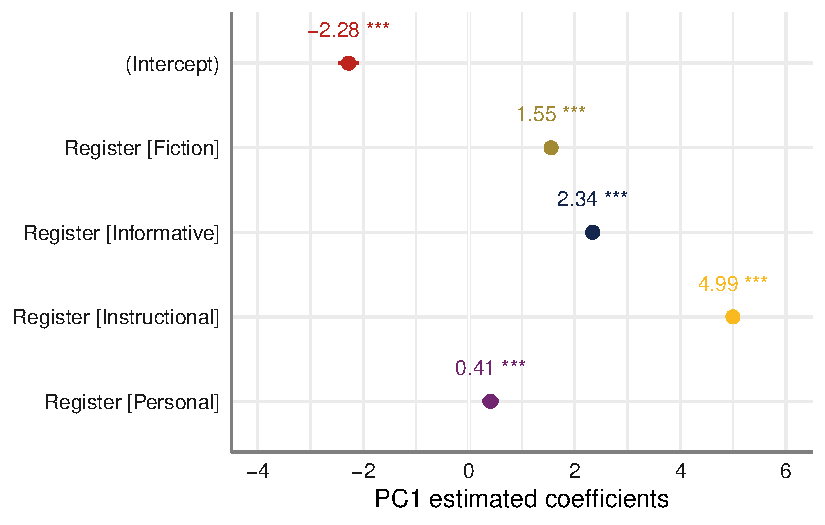
\includegraphics[keepaspectratio]{AppendixF_files/figure-pdf/Dim1fixed-1.pdf}}

\begin{Shaded}
\begin{Highlighting}[]
\CommentTok{\#ggsave(here("plots", "TxB\_PCA1\_lmer\_fixedeffects\_Register.svg"), height = 3, width = 8)}
\end{Highlighting}
\end{Shaded}

The \texttt{emmeans} and \texttt{pairs} functions are used to compare
the estimated Dim1 scores for each register and to compare these to one
another.

\begin{Shaded}
\begin{Highlighting}[]
\NormalTok{Register\_results }\OtherTok{\textless{}{-}} \FunctionTok{emmeans}\NormalTok{(md1Register, }\StringTok{"Register"}\NormalTok{)}
\FunctionTok{summary}\NormalTok{(Register\_results)}
\end{Highlighting}
\end{Shaded}

\begin{verbatim}
 Register       emmean    SE   df lower.CL upper.CL
 Conversation  -2.2793 0.102 11.6   -2.502   -2.056
 Fiction       -0.7267 0.106 13.9   -0.955   -0.498
 Informative    0.0603 0.104 12.7   -0.165    0.286
 Instructional  2.7141 0.101 11.3    2.492    2.937
 Personal      -1.8734 0.122 25.5   -2.125   -1.622

Degrees-of-freedom method: kenward-roger 
Confidence level used: 0.95 
\end{verbatim}

\begin{Shaded}
\begin{Highlighting}[]
\NormalTok{comparisons }\OtherTok{\textless{}{-}} \FunctionTok{pairs}\NormalTok{(Register\_results, }\AttributeTok{adjust =} \StringTok{"tukey"}\NormalTok{)}
\NormalTok{comparisons}
\end{Highlighting}
\end{Shaded}

\begin{verbatim}
 contrast                     estimate     SE   df  t.ratio p.value
 Conversation - Fiction         -1.553 0.0508 1963  -30.535  <.0001
 Conversation - Informative     -2.340 0.0465 1961  -50.341  <.0001
 Conversation - Instructional   -4.993 0.0399 1961 -125.141  <.0001
 Conversation - Personal        -0.406 0.0791 1958   -5.134  <.0001
 Fiction - Informative          -0.787 0.0557 1962  -14.135  <.0001
 Fiction - Instructional        -3.441 0.0497 1962  -69.168  <.0001
 Fiction - Personal              1.147 0.0840 1958   13.645  <.0001
 Informative - Instructional    -2.654 0.0447 1957  -59.399  <.0001
 Informative - Personal          1.934 0.0816 1957   23.692  <.0001
 Instructional - Personal        4.587 0.0780 1957   58.820  <.0001

Degrees-of-freedom method: kenward-roger 
P value adjustment: tukey method for comparing a family of 5 estimates 
\end{verbatim}

\begin{Shaded}
\begin{Highlighting}[]
\CommentTok{\#write\_last\_clip()}
\FunctionTok{confint}\NormalTok{(comparisons)}
\end{Highlighting}
\end{Shaded}

\begin{verbatim}
 contrast                     estimate     SE   df lower.CL upper.CL
 Conversation - Fiction         -1.553 0.0508 1963   -1.691   -1.414
 Conversation - Informative     -2.340 0.0465 1961   -2.466   -2.213
 Conversation - Instructional   -4.993 0.0399 1961   -5.102   -4.884
 Conversation - Personal        -0.406 0.0791 1958   -0.622   -0.190
 Fiction - Informative          -0.787 0.0557 1962   -0.939   -0.635
 Fiction - Instructional        -3.441 0.0497 1962   -3.577   -3.305
 Fiction - Personal              1.147 0.0840 1958    0.917    1.376
 Informative - Instructional    -2.654 0.0447 1957   -2.776   -2.532
 Informative - Personal          1.934 0.0816 1957    1.711    2.156
 Instructional - Personal        4.587 0.0780 1957    4.374    4.800

Degrees-of-freedom method: kenward-roger 
Confidence level used: 0.95 
Conf-level adjustment: tukey method for comparing a family of 5 estimates 
\end{verbatim}

\begin{Shaded}
\begin{Highlighting}[]
\CommentTok{\#write\_last\_clip()}
\end{Highlighting}
\end{Shaded}

We can also visualise the estimated coefficients for the textbook
series, which is modelled here as a random effect.

\begin{Shaded}
\begin{Highlighting}[]
\FunctionTok{plot\_model}\NormalTok{(md1, }
           \AttributeTok{type =} \StringTok{"re"}\NormalTok{, }\CommentTok{\# Option to visualise random effects}
           \AttributeTok{show.values=}\ConstantTok{TRUE}\NormalTok{, }
           \AttributeTok{show.p=}\ConstantTok{TRUE}\NormalTok{,}
           \AttributeTok{value.offset =}\NormalTok{ .}\DecValTok{4}\NormalTok{,}
           \AttributeTok{value.size =} \FloatTok{3.5}\NormalTok{,}
           \AttributeTok{colors =} \StringTok{"bw"}\NormalTok{,}
           \AttributeTok{wrap.labels =} \DecValTok{40}\NormalTok{,}
           \AttributeTok{axis.title =} \StringTok{"PC1 estimated coefficients"}\NormalTok{) }\SpecialCharTok{+}
  \FunctionTok{theme\_sjplot2}\NormalTok{()}
\end{Highlighting}
\end{Shaded}

\pandocbounded{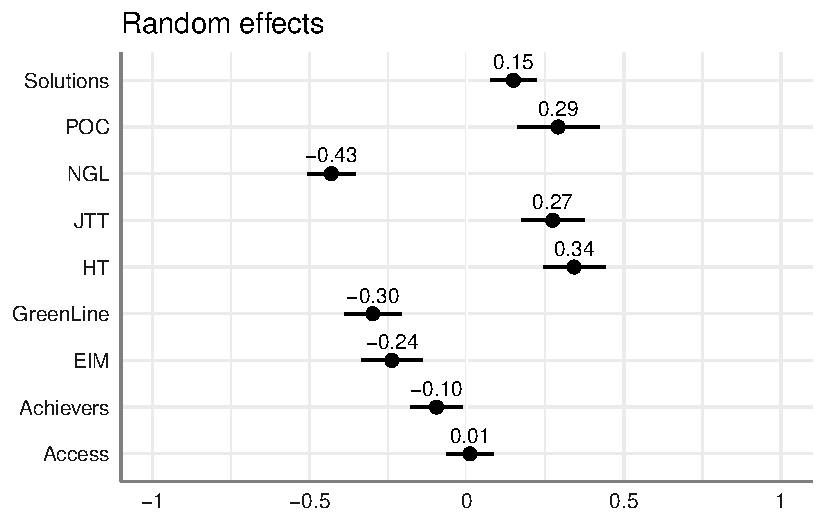
\includegraphics[keepaspectratio]{AppendixF_files/figure-pdf/Dim1random-1.pdf}}

\begin{Shaded}
\begin{Highlighting}[]
\CommentTok{\#ggsave(here("plots", "TxB\_PCA1\_lmer\_randomeffects.svg"), height = 3, width = 8)}
\end{Highlighting}
\end{Shaded}

\subsection{Dimension 2: `Involved vs.~Informational
Production'}\label{dimension-2-involved-vs.-informational-production}

\begin{Shaded}
\begin{Highlighting}[]
\NormalTok{md2 }\OtherTok{\textless{}{-}} \FunctionTok{lmer}\NormalTok{(PC2 }\SpecialCharTok{\textasciitilde{}}\NormalTok{ Register}\SpecialCharTok{*}\NormalTok{Level }\SpecialCharTok{+}\NormalTok{ (}\DecValTok{1}\SpecialCharTok{|}\NormalTok{Series), }\AttributeTok{data =}\NormalTok{ res.ind, }\AttributeTok{REML =} \ConstantTok{FALSE}\NormalTok{)}
\NormalTok{md2Register }\OtherTok{\textless{}{-}} \FunctionTok{lmer}\NormalTok{(PC2 }\SpecialCharTok{\textasciitilde{}}\NormalTok{ Register }\SpecialCharTok{+}\NormalTok{ (}\DecValTok{1}\SpecialCharTok{|}\NormalTok{Series), }\AttributeTok{data =}\NormalTok{ res.ind, }\AttributeTok{REML =} \ConstantTok{FALSE}\NormalTok{)}
\NormalTok{md2Level }\OtherTok{\textless{}{-}} \FunctionTok{lmer}\NormalTok{(PC2 }\SpecialCharTok{\textasciitilde{}}\NormalTok{ Level }\SpecialCharTok{+}\NormalTok{ (}\DecValTok{1}\SpecialCharTok{|}\NormalTok{Series), }\AttributeTok{data =}\NormalTok{ res.ind, }\AttributeTok{REML =} \ConstantTok{FALSE}\NormalTok{)}
\FunctionTok{anova}\NormalTok{(md2, md2Register, md2Level)}
\end{Highlighting}
\end{Shaded}

\begin{verbatim}
Data: res.ind
Models:
md2Register: PC2 ~ Register + (1 | Series)
md2Level: PC2 ~ Level + (1 | Series)
md2: PC2 ~ Register * Level + (1 | Series)
            npar    AIC    BIC  logLik deviance  Chisq Df Pr(>Chisq)    
md2Register    7 6155.2 6194.3 -3070.6   6141.2                         
md2Level       7 7290.1 7329.2 -3638.1   7276.1    0.0  0               
md2           27 5200.9 5351.6 -2573.4   5146.9 2129.2 20  < 2.2e-16 ***
---
Signif. codes:  0 '***' 0.001 '**' 0.01 '*' 0.05 '.' 0.1 ' ' 1
\end{verbatim}

\begin{Shaded}
\begin{Highlighting}[]
\FunctionTok{tab\_model}\NormalTok{(md2) }\CommentTok{\# Marginal R2 = 0.723}
\end{Highlighting}
\end{Shaded}

\begin{Shaded}
\begin{Highlighting}[]
\CommentTok{\# tab\_model(md2Register) \# Marginal R2 = 0.558}
\CommentTok{\# tab\_model(md2Level) \# Marginal R2 = 0.228}
\end{Highlighting}
\end{Shaded}

Estimated coefficients of fixed effects on Dim2 scores:

\begin{Shaded}
\begin{Highlighting}[]
\FunctionTok{plot\_model}\NormalTok{(md2, }
           \AttributeTok{type =} \StringTok{"est"}\NormalTok{,}
           \AttributeTok{show.intercept =} \ConstantTok{TRUE}\NormalTok{,}
           \AttributeTok{show.values=}\ConstantTok{TRUE}\NormalTok{, }
           \AttributeTok{show.p=}\ConstantTok{TRUE}\NormalTok{,}
           \AttributeTok{value.offset =}\NormalTok{ .}\DecValTok{4}\NormalTok{,}
           \AttributeTok{value.size =} \FloatTok{3.5}\NormalTok{,}
           \AttributeTok{colors =}\NormalTok{ palette[}\FunctionTok{c}\NormalTok{(}\DecValTok{1}\SpecialCharTok{:}\DecValTok{3}\NormalTok{,}\DecValTok{8}\NormalTok{,}\DecValTok{7}\NormalTok{)],}
           \AttributeTok{group.terms =} \FunctionTok{c}\NormalTok{(}\DecValTok{1}\SpecialCharTok{:}\DecValTok{5}\NormalTok{,}\DecValTok{1}\NormalTok{,}\DecValTok{1}\NormalTok{,}\DecValTok{1}\NormalTok{,}\DecValTok{1}\NormalTok{,}\DecValTok{2}\SpecialCharTok{:}\DecValTok{5}\NormalTok{,}\DecValTok{2}\SpecialCharTok{:}\DecValTok{5}\NormalTok{,}\DecValTok{2}\SpecialCharTok{:}\DecValTok{5}\NormalTok{,}\DecValTok{2}\SpecialCharTok{:}\DecValTok{5}\NormalTok{), }
           \AttributeTok{title =} \StringTok{""}\NormalTok{,}
           \AttributeTok{wrap.labels =} \DecValTok{40}\NormalTok{,}
           \AttributeTok{axis.title =} \StringTok{"PC2 estimated coefficients"}\NormalTok{) }\SpecialCharTok{+}
  \FunctionTok{theme\_sjplot2}\NormalTok{() }
\end{Highlighting}
\end{Shaded}

\pandocbounded{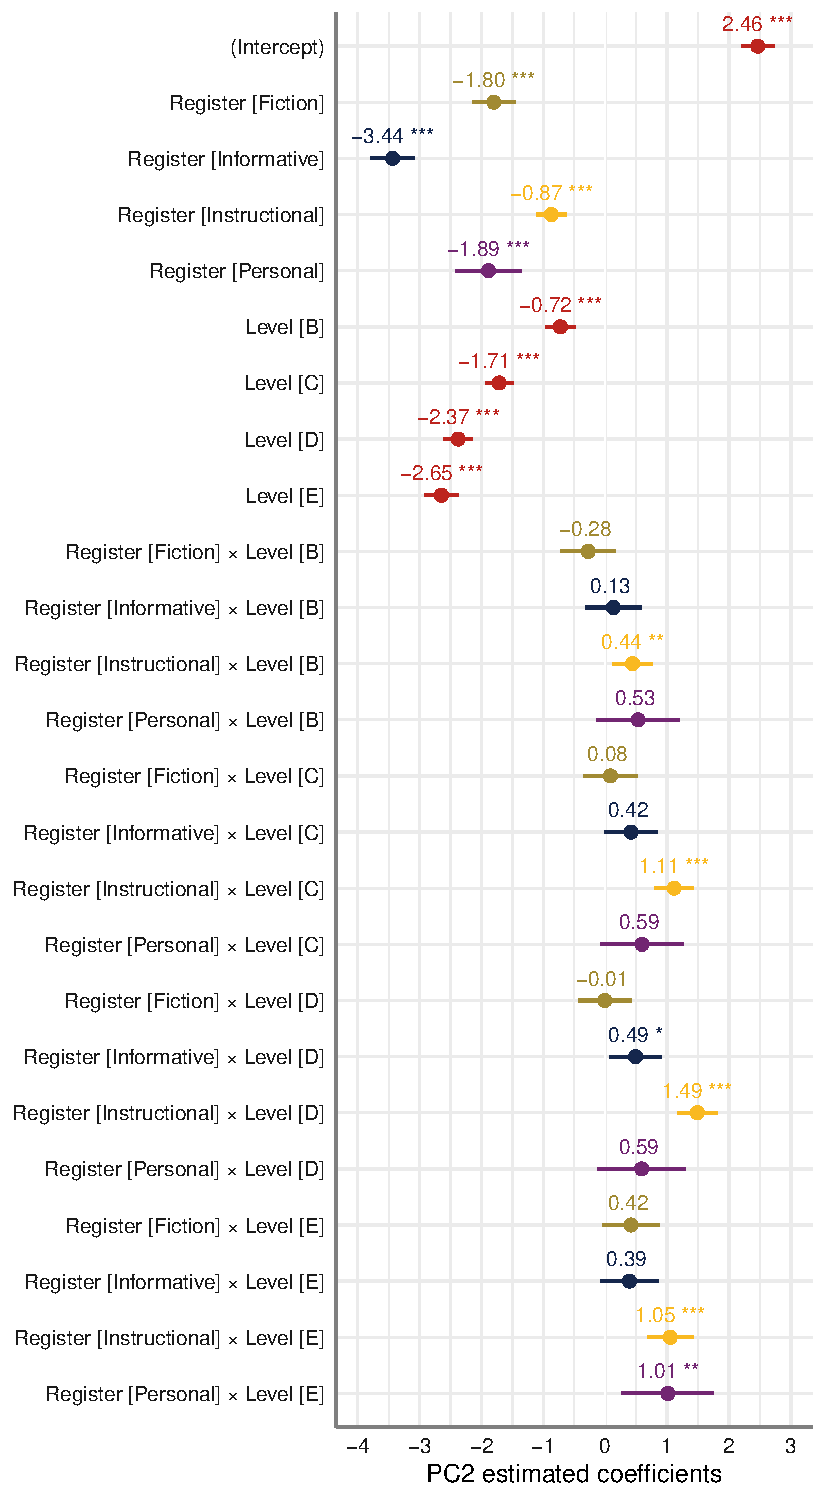
\includegraphics[keepaspectratio]{AppendixF_files/figure-pdf/Dim2fixed-1.pdf}}

\begin{Shaded}
\begin{Highlighting}[]
\CommentTok{\#ggsave(here("plots", "TxB\_PCA2\_lmer\_fixedeffects.svg"), height = 8, width = 8)}
\end{Highlighting}
\end{Shaded}

Estimated coefficients of random effects on Dim2 scores:

\begin{Shaded}
\begin{Highlighting}[]
\DocumentationTok{\#\# Random intercepts}
\FunctionTok{plot\_model}\NormalTok{(md2, }
           \AttributeTok{type =} \StringTok{"re"}\NormalTok{, }\CommentTok{\# Option to visualise random effects}
           \AttributeTok{show.values=}\ConstantTok{TRUE}\NormalTok{, }
           \AttributeTok{show.p=}\ConstantTok{TRUE}\NormalTok{,}
           \AttributeTok{value.offset =}\NormalTok{ .}\DecValTok{4}\NormalTok{,}
           \AttributeTok{value.size =} \FloatTok{3.5}\NormalTok{,}
           \AttributeTok{colors =} \StringTok{"bw"}\NormalTok{,}
           \AttributeTok{wrap.labels =} \DecValTok{40}\NormalTok{,}
           \AttributeTok{axis.title =} \StringTok{"PC2 estimated coefficients"}\NormalTok{) }\SpecialCharTok{+}
  \FunctionTok{theme\_sjplot2}\NormalTok{()}
\end{Highlighting}
\end{Shaded}

\pandocbounded{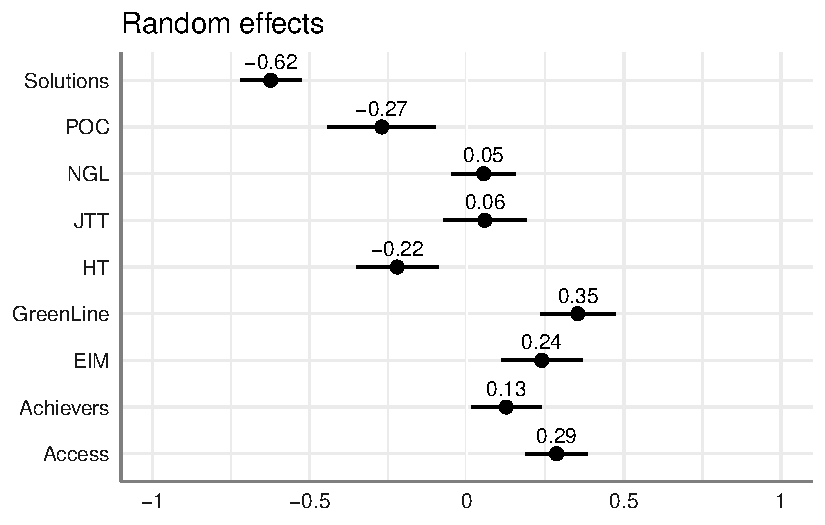
\includegraphics[keepaspectratio]{AppendixF_files/figure-pdf/Dim2random-1.pdf}}

\begin{Shaded}
\begin{Highlighting}[]
\CommentTok{\#ggsave(here("plots", "TxB\_PCA2\_lmer\_randomeffects.svg"), height = 3, width = 8)}

\CommentTok{\# Textbook Country as a random effect variable}
\NormalTok{md2country }\OtherTok{\textless{}{-}} \FunctionTok{lmer}\NormalTok{(PC2 }\SpecialCharTok{\textasciitilde{}}\NormalTok{ Register}\SpecialCharTok{*}\NormalTok{Level }\SpecialCharTok{+}\NormalTok{ (}\DecValTok{1}\SpecialCharTok{|}\NormalTok{Country), }\AttributeTok{data =}\NormalTok{ res.ind, }\AttributeTok{REML =} \ConstantTok{FALSE}\NormalTok{)}

\FunctionTok{plot\_model}\NormalTok{(md2country, }
           \AttributeTok{type =} \StringTok{"re"}\NormalTok{, }\CommentTok{\# Option to visualise random effects}
           \AttributeTok{show.values=}\ConstantTok{TRUE}\NormalTok{, }
           \AttributeTok{show.p=}\ConstantTok{TRUE}\NormalTok{,}
           \AttributeTok{value.offset =}\NormalTok{ .}\DecValTok{4}\NormalTok{,}
           \AttributeTok{value.size =} \FloatTok{3.5}\NormalTok{,}
           \AttributeTok{colors =} \StringTok{"bw"}\NormalTok{,}
           \AttributeTok{wrap.labels =} \DecValTok{40}\NormalTok{,}
           \AttributeTok{axis.title =} \StringTok{"PC2 estimated coefficients"}\NormalTok{) }\SpecialCharTok{+}
  \FunctionTok{theme\_sjplot2}\NormalTok{()}
\end{Highlighting}
\end{Shaded}

\pandocbounded{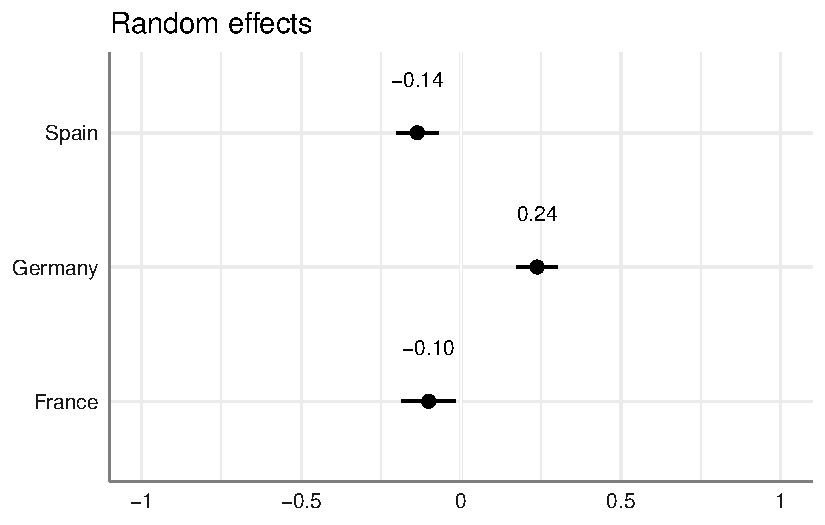
\includegraphics[keepaspectratio]{AppendixF_files/figure-pdf/Dim2random-2.pdf}}

\begin{Shaded}
\begin{Highlighting}[]
\CommentTok{\#ggsave(here("plots", "TxB\_PCA2\_lmer\_randomeffects\_country.svg"), height = 3, width = 8)}
\end{Highlighting}
\end{Shaded}

The \texttt{visreg} function is used to visualise the distributions of
the modelled Dim2 scores.

\begin{Shaded}
\begin{Highlighting}[]
\CommentTok{\# svg(here("plots", "TxB\_predicted\_PC2\_scores\_interactions.svg"), height = 5, width = 8)}
\FunctionTok{visreg}\NormalTok{(md2, }\AttributeTok{xvar =} \StringTok{"Level"}\NormalTok{, }\AttributeTok{by=}\StringTok{"Register"}\NormalTok{, }\AttributeTok{type =} \StringTok{"conditional"}\NormalTok{,}
       \AttributeTok{line=}\FunctionTok{list}\NormalTok{(}\AttributeTok{col=}\StringTok{"darkred"}\NormalTok{), }
       \AttributeTok{xlab =} \StringTok{"Textbook Level"}\NormalTok{, }\AttributeTok{ylab =} \StringTok{"PC2"}
       \CommentTok{\#,gg = TRUE}
\NormalTok{       ,}\AttributeTok{layout=}\FunctionTok{c}\NormalTok{(}\DecValTok{5}\NormalTok{,}\DecValTok{1}\NormalTok{)}
\NormalTok{)}
\end{Highlighting}
\end{Shaded}

\pandocbounded{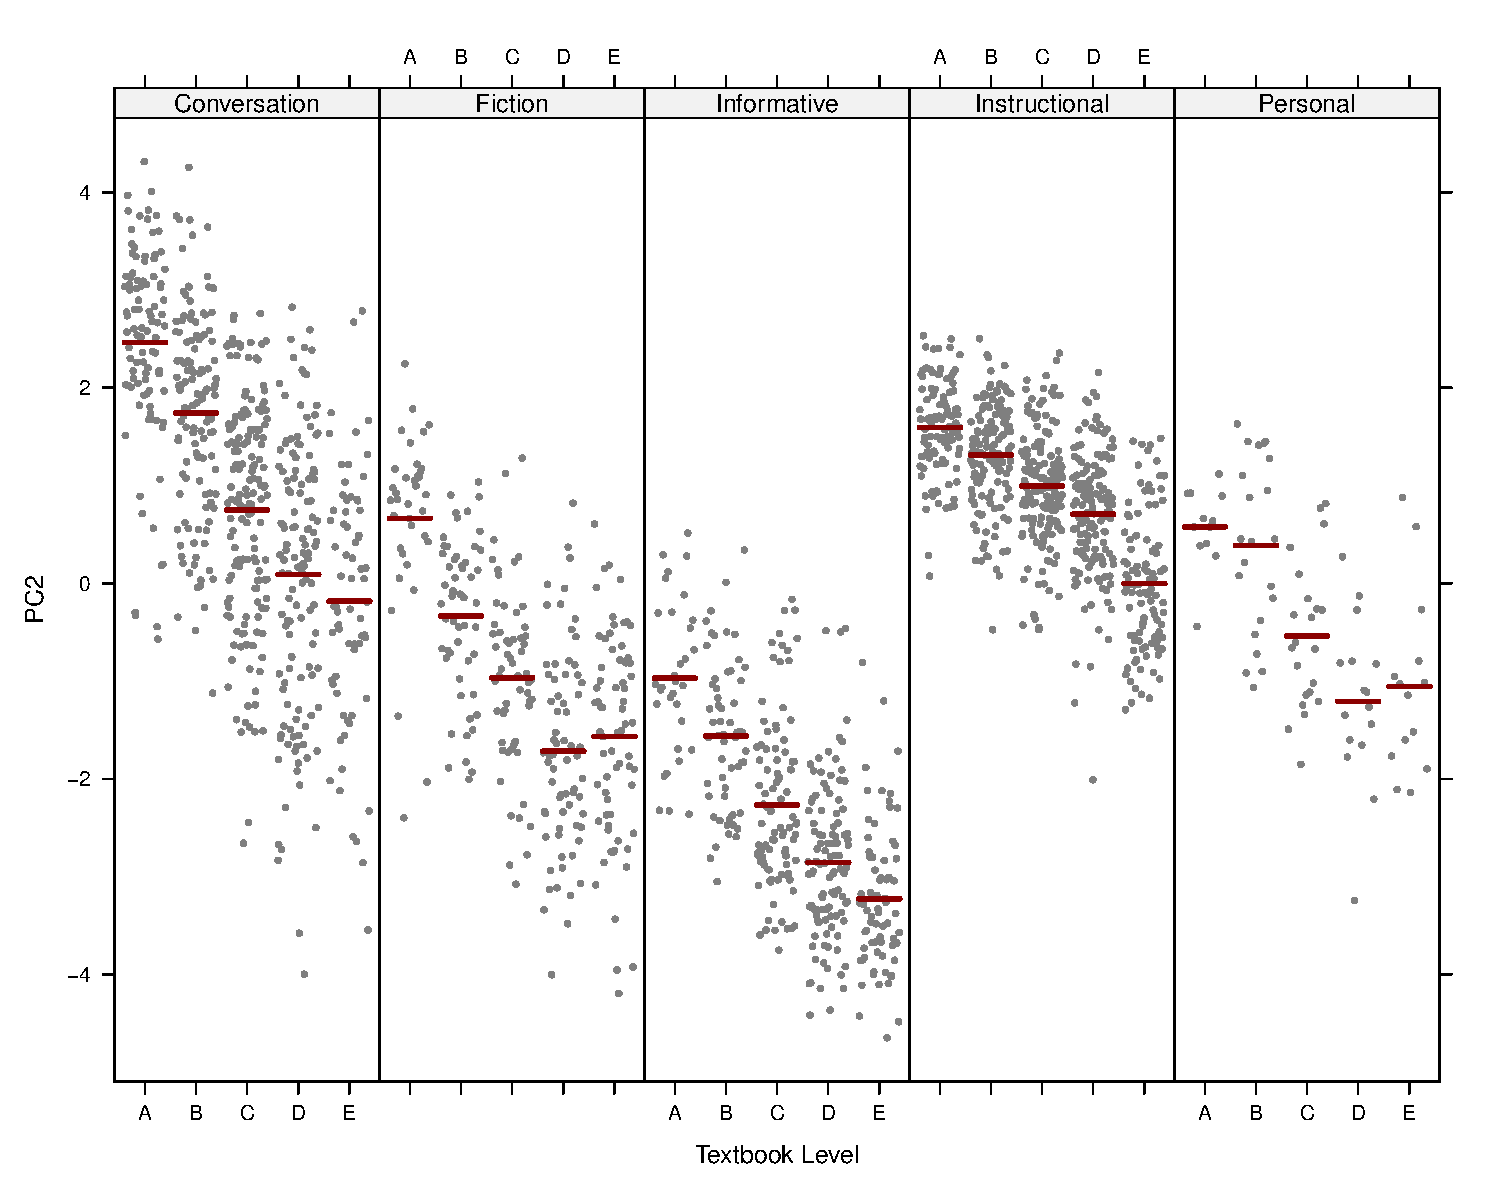
\includegraphics[keepaspectratio]{AppendixF_files/figure-pdf/Dim2estimateplots-1.pdf}}

\begin{Shaded}
\begin{Highlighting}[]
\CommentTok{\#dev.off()}
\end{Highlighting}
\end{Shaded}

We also examine potential interactions between textbook series,
proficiency level, and Dim2 scores.

\begin{Shaded}
\begin{Highlighting}[]
\FunctionTok{visreg}\NormalTok{(md2, }\AttributeTok{xvar =} \StringTok{"Series"}\NormalTok{, }\AttributeTok{by=}\StringTok{"Level"}\NormalTok{, }\AttributeTok{type =} \StringTok{"conditional"}\NormalTok{, }\AttributeTok{re.form=}\SpecialCharTok{\textasciitilde{}}\NormalTok{(}\DecValTok{1}\SpecialCharTok{|}\NormalTok{Series), }
       \AttributeTok{line=}\FunctionTok{list}\NormalTok{(}\AttributeTok{col=}\StringTok{"darkred"}\NormalTok{), }\AttributeTok{xlab =} \StringTok{"Textbook Series"}\NormalTok{, }\AttributeTok{ylab =} \StringTok{"PC2"}\NormalTok{,}
       \AttributeTok{layout=}\FunctionTok{c}\NormalTok{(}\DecValTok{1}\NormalTok{,}\DecValTok{5}\NormalTok{))}
\end{Highlighting}
\end{Shaded}

\pandocbounded{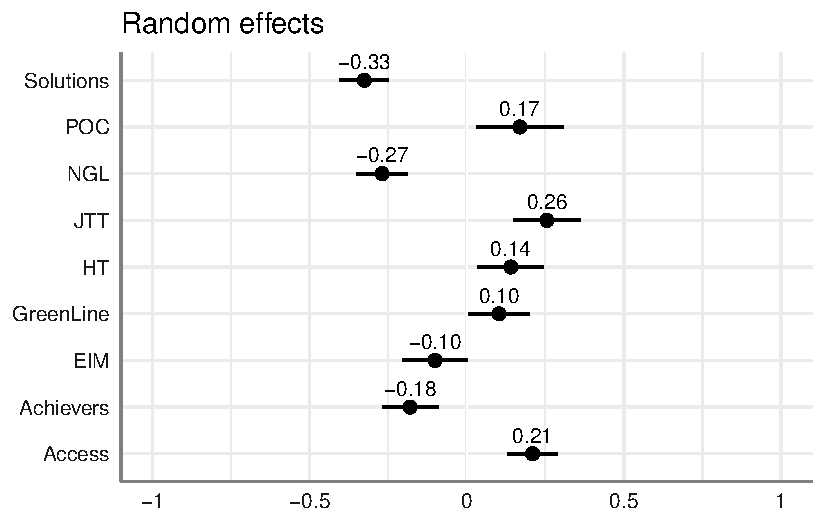
\includegraphics[keepaspectratio]{AppendixF_files/figure-pdf/unnamed-chunk-31-1.pdf}}

Finally, we examine potential interactions between country of use of the
textbook, register, and Dim2 scores.

\begin{Shaded}
\begin{Highlighting}[]
\CommentTok{\# svg(here("plots", "TxB\_PCA2\_lmer\_randomeffects\_country\_register.svg"), height = 5, width = 8)}
\NormalTok{visreg}\SpecialCharTok{::}\FunctionTok{visreg}\NormalTok{(md2country, }\StringTok{"Country"}\NormalTok{, }\AttributeTok{by=}\StringTok{"Register"}\NormalTok{, }\AttributeTok{re.form=}\SpecialCharTok{\textasciitilde{}}\NormalTok{(}\DecValTok{1}\SpecialCharTok{|}\NormalTok{Country),}
               \AttributeTok{ylab=}\StringTok{"PC2"}\NormalTok{, }\AttributeTok{line=}\FunctionTok{list}\NormalTok{(}\AttributeTok{col=}\StringTok{"darkred"}\NormalTok{))}
\end{Highlighting}
\end{Shaded}

\pandocbounded{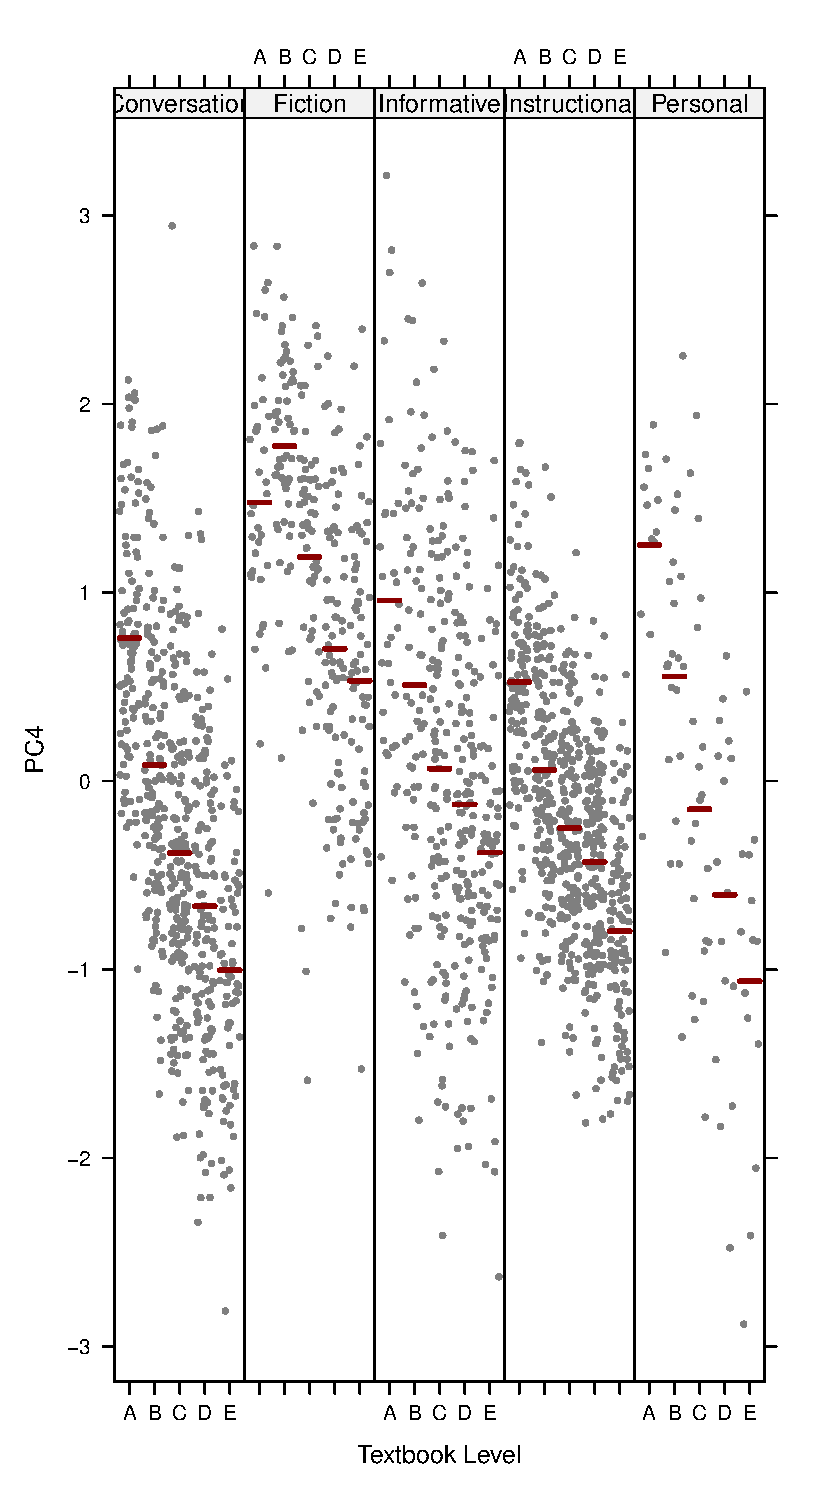
\includegraphics[keepaspectratio]{AppendixF_files/figure-pdf/unnamed-chunk-32-1.pdf}}

\begin{Shaded}
\begin{Highlighting}[]
\CommentTok{\# dev.off()}
\end{Highlighting}
\end{Shaded}

\subsection{Dimension 3: `Narrative vs.~factual
discourse'}\label{dimension-3-narrative-vs.-factual-discourse}

\begin{Shaded}
\begin{Highlighting}[]
\NormalTok{md3 }\OtherTok{\textless{}{-}} \FunctionTok{lmer}\NormalTok{(PC3 }\SpecialCharTok{\textasciitilde{}}\NormalTok{ Register}\SpecialCharTok{*}\NormalTok{Level }\SpecialCharTok{+}\NormalTok{ (}\DecValTok{1}\SpecialCharTok{|}\NormalTok{Series), }\AttributeTok{data =}\NormalTok{ res.ind, }\AttributeTok{REML =} \ConstantTok{FALSE}\NormalTok{)}
\NormalTok{md3Register }\OtherTok{\textless{}{-}} \FunctionTok{lmer}\NormalTok{(PC3 }\SpecialCharTok{\textasciitilde{}}\NormalTok{ Register }\SpecialCharTok{+}\NormalTok{ (}\DecValTok{1}\SpecialCharTok{|}\NormalTok{Series), }\AttributeTok{data =}\NormalTok{ res.ind, }\AttributeTok{REML =} \ConstantTok{FALSE}\NormalTok{)}
\NormalTok{md3Level }\OtherTok{\textless{}{-}} \FunctionTok{lmer}\NormalTok{(PC3 }\SpecialCharTok{\textasciitilde{}}\NormalTok{ Level }\SpecialCharTok{+}\NormalTok{ (}\DecValTok{1}\SpecialCharTok{|}\NormalTok{Series), }\AttributeTok{data =}\NormalTok{ res.ind, }\AttributeTok{REML =} \ConstantTok{FALSE}\NormalTok{)}

\FunctionTok{anova}\NormalTok{(md3, md3Register, md3Level)}
\end{Highlighting}
\end{Shaded}

\begin{verbatim}
Data: res.ind
Models:
md3Register: PC3 ~ Register + (1 | Series)
md3Level: PC3 ~ Level + (1 | Series)
md3: PC3 ~ Register * Level + (1 | Series)
            npar    AIC    BIC  logLik deviance  Chisq Df Pr(>Chisq)    
md3Register    7 5139.9 5179.0 -2563.0   5125.9                         
md3Level       7 5528.8 5567.9 -2757.4   5514.8   0.00  0               
md3           27 4582.6 4733.3 -2264.3   4528.6 986.21 20  < 2.2e-16 ***
---
Signif. codes:  0 '***' 0.001 '**' 0.01 '*' 0.05 '.' 0.1 ' ' 1
\end{verbatim}

\begin{Shaded}
\begin{Highlighting}[]
\FunctionTok{tab\_model}\NormalTok{(md3) }\CommentTok{\# Marginal R2 = 0.436}
\end{Highlighting}
\end{Shaded}

\begin{Shaded}
\begin{Highlighting}[]
\CommentTok{\# tab\_model(md3Register) \# Marginal R2 = 0.272}
\CommentTok{\# tab\_model(md3Level) \# Marginal R2 = 0.119}

\CommentTok{\# Plot of fixed effects:}
\FunctionTok{plot\_model}\NormalTok{(md3, }
           \AttributeTok{type =} \StringTok{"est"}\NormalTok{,}
           \AttributeTok{show.intercept =} \ConstantTok{TRUE}\NormalTok{,}
           \AttributeTok{show.values=}\ConstantTok{TRUE}\NormalTok{, }
           \AttributeTok{show.p=}\ConstantTok{TRUE}\NormalTok{,}
           \AttributeTok{value.offset =}\NormalTok{ .}\DecValTok{4}\NormalTok{,}
           \AttributeTok{value.size =} \FloatTok{3.5}\NormalTok{,}
           \AttributeTok{colors =}\NormalTok{ palette[}\FunctionTok{c}\NormalTok{(}\DecValTok{1}\SpecialCharTok{:}\DecValTok{3}\NormalTok{,}\DecValTok{8}\NormalTok{,}\DecValTok{7}\NormalTok{)],}
           \AttributeTok{group.terms =} \FunctionTok{c}\NormalTok{(}\DecValTok{1}\SpecialCharTok{:}\DecValTok{5}\NormalTok{,}\DecValTok{1}\NormalTok{,}\DecValTok{1}\NormalTok{,}\DecValTok{1}\NormalTok{,}\DecValTok{1}\NormalTok{,}\DecValTok{2}\SpecialCharTok{:}\DecValTok{5}\NormalTok{,}\DecValTok{2}\SpecialCharTok{:}\DecValTok{5}\NormalTok{,}\DecValTok{2}\SpecialCharTok{:}\DecValTok{5}\NormalTok{,}\DecValTok{2}\SpecialCharTok{:}\DecValTok{5}\NormalTok{), }
           \AttributeTok{title =} \StringTok{""}\NormalTok{,}
           \AttributeTok{wrap.labels =} \DecValTok{40}\NormalTok{,}
           \AttributeTok{axis.title =} \StringTok{"PC3 estimated coefficients"}\NormalTok{) }\SpecialCharTok{+}
  \FunctionTok{theme\_sjplot2}\NormalTok{() }
\end{Highlighting}
\end{Shaded}

\pandocbounded{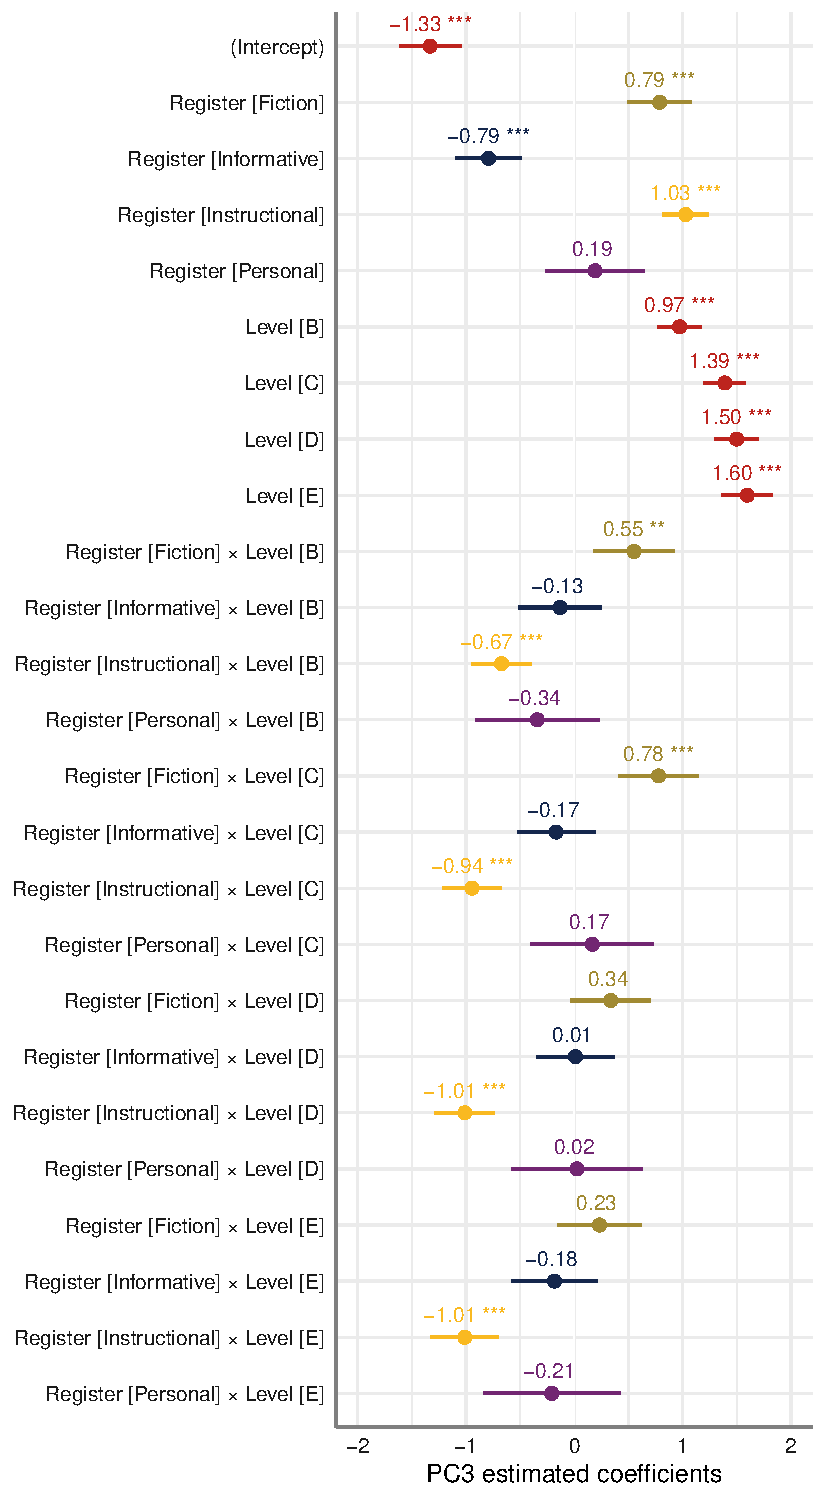
\includegraphics[keepaspectratio]{AppendixF_files/figure-pdf/Dim3model-1.pdf}}

\begin{Shaded}
\begin{Highlighting}[]
\CommentTok{\#ggsave(here("plots", "TxB\_PCA3\_lmer\_fixedeffects.svg"), height = 8, width = 8)}
\end{Highlighting}
\end{Shaded}

\begin{Shaded}
\begin{Highlighting}[]
\CommentTok{\# Plot of random effects:}
\FunctionTok{plot\_model}\NormalTok{(md3, }
           \AttributeTok{type =} \StringTok{"re"}\NormalTok{, }\CommentTok{\# Option to visualise random effects}
           \AttributeTok{show.values=}\ConstantTok{TRUE}\NormalTok{, }
           \AttributeTok{show.p=}\ConstantTok{TRUE}\NormalTok{,}
           \AttributeTok{value.offset =}\NormalTok{ .}\DecValTok{4}\NormalTok{,}
           \AttributeTok{value.size =} \FloatTok{3.5}\NormalTok{,}
           \AttributeTok{color =} \StringTok{"bw"}\NormalTok{,}
           \AttributeTok{wrap.labels =} \DecValTok{40}\NormalTok{,}
           \AttributeTok{axis.title =} \StringTok{"PC3 estimated coefficients"}\NormalTok{) }\SpecialCharTok{+}
  \FunctionTok{theme\_sjplot2}\NormalTok{()}
\end{Highlighting}
\end{Shaded}

\pandocbounded{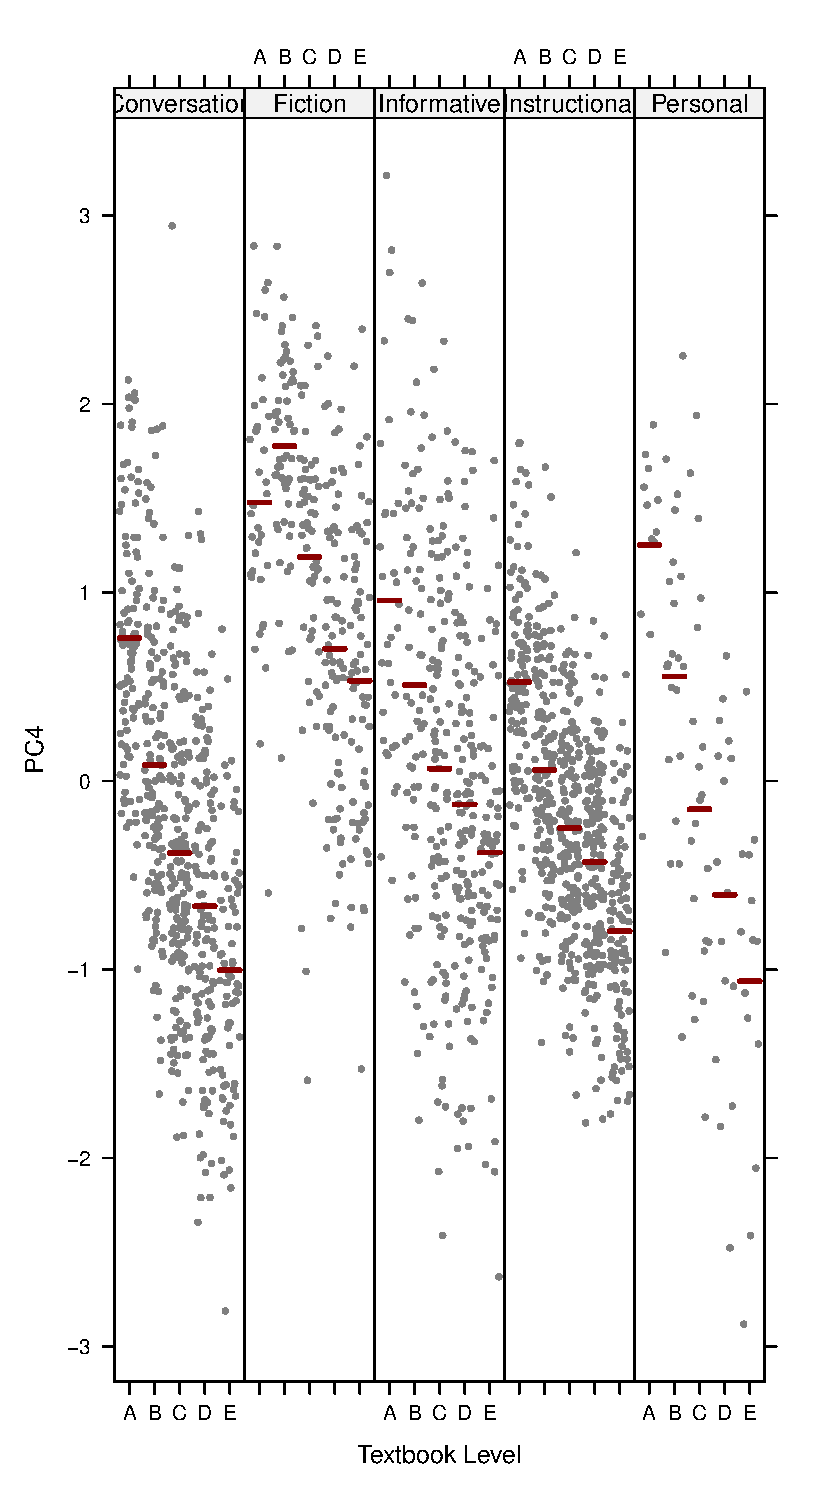
\includegraphics[keepaspectratio]{AppendixF_files/figure-pdf/unnamed-chunk-34-1.pdf}}

\begin{Shaded}
\begin{Highlighting}[]
\CommentTok{\#ggsave(here("plots", "TxB\_PCA3\_lmer\_randomeffects.svg"), height = 3, width = 8)}
\end{Highlighting}
\end{Shaded}

\begin{Shaded}
\begin{Highlighting}[]
\CommentTok{\# svg(here("plots", "TxB\_predicted\_PC3\_scores\_interactions.svg"), height = 5, width = 8)}
\FunctionTok{visreg}\NormalTok{(md3, }\AttributeTok{xvar =} \StringTok{"Level"}\NormalTok{, }\AttributeTok{by=}\StringTok{"Register"}\NormalTok{, }\AttributeTok{type =} \StringTok{"conditional"}\NormalTok{,}
       \AttributeTok{line=}\FunctionTok{list}\NormalTok{(}\AttributeTok{col=}\StringTok{"darkred"}\NormalTok{), }
       \AttributeTok{xlab =} \StringTok{"Textbook Level"}\NormalTok{, }\AttributeTok{ylab =} \StringTok{"PC3"}
       \CommentTok{\#,gg = TRUE}
\NormalTok{       ,}\AttributeTok{layout=}\FunctionTok{c}\NormalTok{(}\DecValTok{5}\NormalTok{,}\DecValTok{1}\NormalTok{)}
\NormalTok{)}
\end{Highlighting}
\end{Shaded}

\pandocbounded{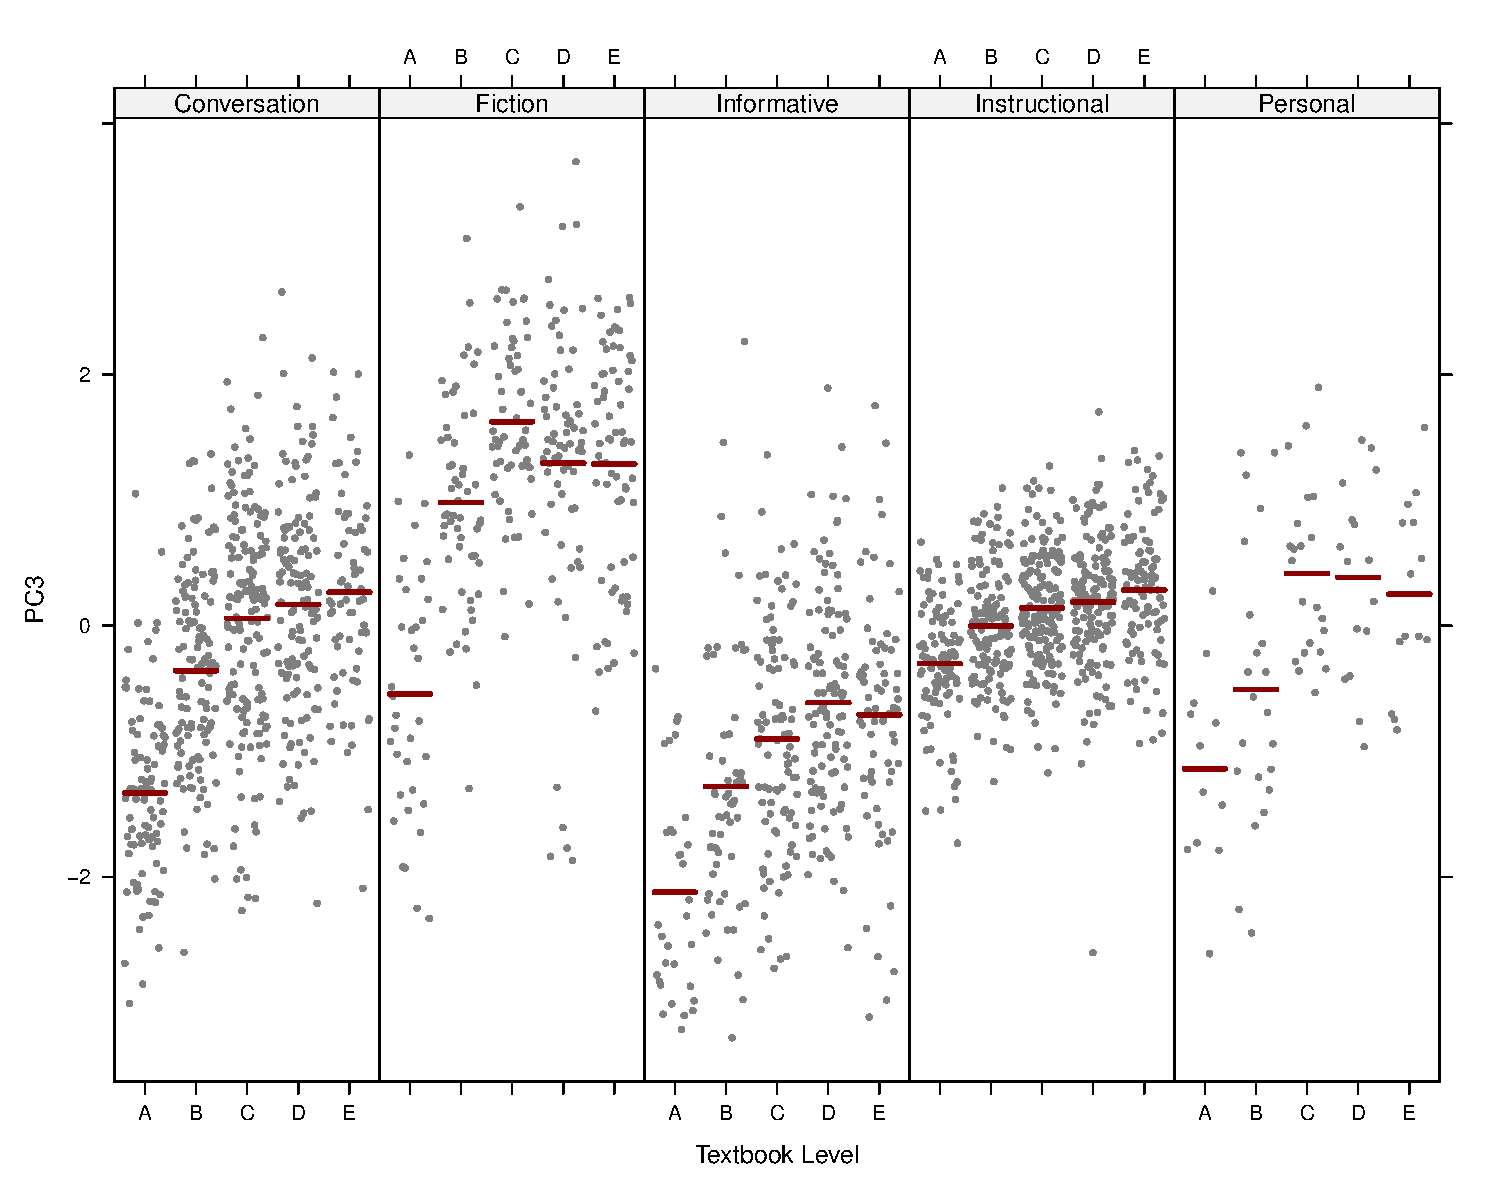
\includegraphics[keepaspectratio]{AppendixF_files/figure-pdf/Dim3comparisons-1.pdf}}

\begin{Shaded}
\begin{Highlighting}[]
\CommentTok{\# dev.off()}

\CommentTok{\# Textbook Series{-}Register interactions}
\NormalTok{visreg}\SpecialCharTok{::}\FunctionTok{visreg}\NormalTok{(md3, }\StringTok{"Series"}\NormalTok{, }\AttributeTok{by=}\StringTok{"Register"}\NormalTok{, }\AttributeTok{re.form=}\SpecialCharTok{\textasciitilde{}}\NormalTok{(}\DecValTok{1}\SpecialCharTok{|}\NormalTok{Series),}
               \AttributeTok{ylab=}\StringTok{"PC3"}\NormalTok{, }\AttributeTok{line=}\FunctionTok{list}\NormalTok{(}\AttributeTok{col=}\StringTok{"darkred"}\NormalTok{))}
\end{Highlighting}
\end{Shaded}

\pandocbounded{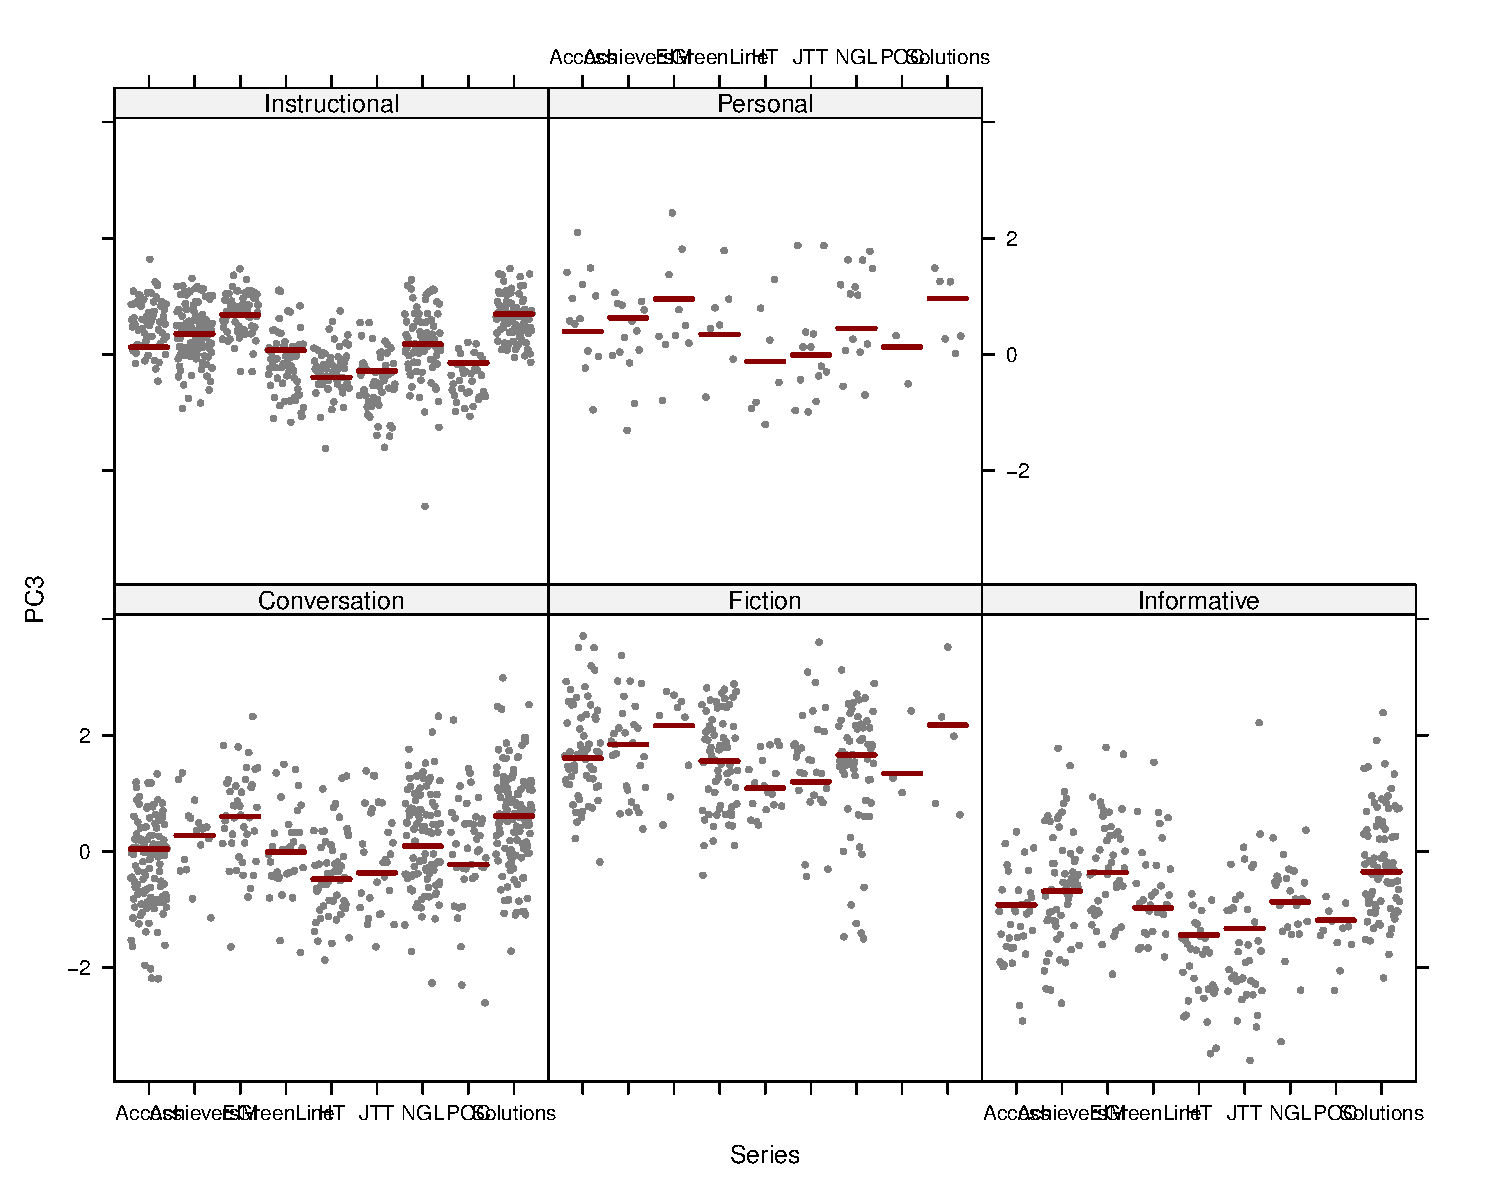
\includegraphics[keepaspectratio]{AppendixF_files/figure-pdf/Dim3comparisons-2.pdf}}

\begin{Shaded}
\begin{Highlighting}[]
\FunctionTok{visreg}\NormalTok{(md3, }\AttributeTok{xvar =} \StringTok{"Level"}\NormalTok{, }\AttributeTok{by=}\StringTok{"Series"}\NormalTok{, }\AttributeTok{type =} \StringTok{"conditional"}\NormalTok{, }\AttributeTok{re.form=}\SpecialCharTok{\textasciitilde{}}\NormalTok{(}\DecValTok{1}\SpecialCharTok{|}\NormalTok{Series), }
       \AttributeTok{line=}\FunctionTok{list}\NormalTok{(}\AttributeTok{col=}\StringTok{"darkred"}\NormalTok{), }\AttributeTok{xlab =} \StringTok{"Textbook Series"}\NormalTok{, }\AttributeTok{ylab =} \StringTok{"PC3"}\NormalTok{)}
\end{Highlighting}
\end{Shaded}

\pandocbounded{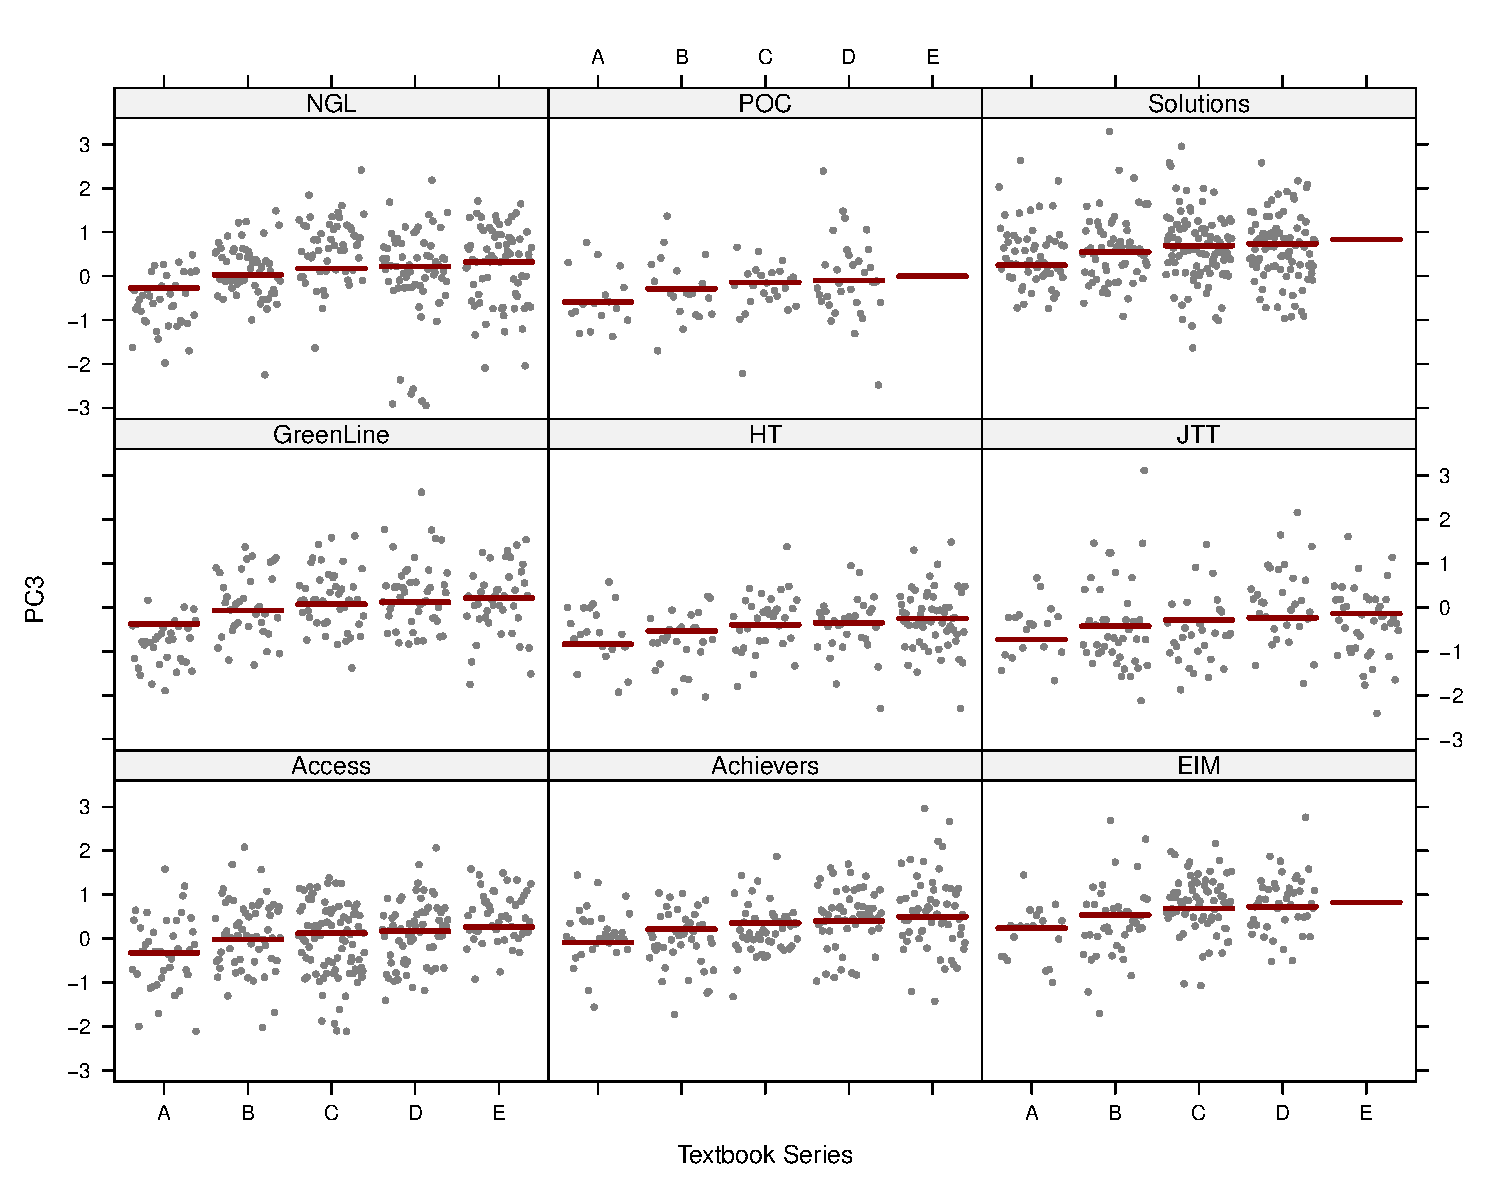
\includegraphics[keepaspectratio]{AppendixF_files/figure-pdf/Dim3comparisons-3.pdf}}

\subsection{Dimension 4: `Informational compression
vs.~elaboration'}\label{dimension-4-informational-compression-vs.-elaboration}

\begin{Shaded}
\begin{Highlighting}[]
\NormalTok{md4 }\OtherTok{\textless{}{-}} \FunctionTok{lmer}\NormalTok{(PC4 }\SpecialCharTok{\textasciitilde{}}\NormalTok{ Register}\SpecialCharTok{*}\NormalTok{Level }\SpecialCharTok{+}\NormalTok{ (}\DecValTok{1}\SpecialCharTok{|}\NormalTok{Series), }\AttributeTok{data =}\NormalTok{ res.ind, }\AttributeTok{REML =} \ConstantTok{FALSE}\NormalTok{)}
\NormalTok{md4Register }\OtherTok{\textless{}{-}} \FunctionTok{lmer}\NormalTok{(PC4 }\SpecialCharTok{\textasciitilde{}}\NormalTok{ Register }\SpecialCharTok{+}\NormalTok{ (}\DecValTok{1}\SpecialCharTok{|}\NormalTok{Series), }\AttributeTok{data =}\NormalTok{ res.ind, }\AttributeTok{REML =} \ConstantTok{FALSE}\NormalTok{)}
\NormalTok{md4Level }\OtherTok{\textless{}{-}} \FunctionTok{lmer}\NormalTok{(PC4 }\SpecialCharTok{\textasciitilde{}}\NormalTok{ Level }\SpecialCharTok{+}\NormalTok{ (}\DecValTok{1}\SpecialCharTok{|}\NormalTok{Series), }\AttributeTok{data =}\NormalTok{ res.ind, }\AttributeTok{REML =} \ConstantTok{FALSE}\NormalTok{)}

\FunctionTok{anova}\NormalTok{(md4, md4Register, md4Level)}
\end{Highlighting}
\end{Shaded}

\begin{verbatim}
Data: res.ind
Models:
md4Register: PC4 ~ Register + (1 | Series)
md4Level: PC4 ~ Level + (1 | Series)
md4: PC4 ~ Register * Level + (1 | Series)
            npar    AIC    BIC  logLik deviance  Chisq Df Pr(>Chisq)    
md4Register    7 5034.0 5073.0 -2510.0   5020.0                         
md4Level       7 5043.6 5082.7 -2514.8   5029.6   0.00  0               
md4           27 4372.1 4522.8 -2159.1   4318.1 711.52 20  < 2.2e-16 ***
---
Signif. codes:  0 '***' 0.001 '**' 0.01 '*' 0.05 '.' 0.1 ' ' 1
\end{verbatim}

\begin{Shaded}
\begin{Highlighting}[]
\FunctionTok{tab\_model}\NormalTok{(md4) }\CommentTok{\# Marginal R2 = 0.426}
\end{Highlighting}
\end{Shaded}

\begin{Shaded}
\begin{Highlighting}[]
\CommentTok{\# tab\_model(md4Register) \# Marginal R2 = 0.203}
\CommentTok{\# tab\_model(md4Level) \# Marginal R2 = 0.187}

\CommentTok{\# Plot of fixed effects:}
\FunctionTok{plot\_model}\NormalTok{(md4, }
           \AttributeTok{type =} \StringTok{"est"}\NormalTok{,}
           \AttributeTok{show.intercept =} \ConstantTok{TRUE}\NormalTok{,}
           \AttributeTok{show.values=}\ConstantTok{TRUE}\NormalTok{, }
           \AttributeTok{show.p=}\ConstantTok{TRUE}\NormalTok{,}
           \AttributeTok{value.offset =}\NormalTok{ .}\DecValTok{4}\NormalTok{,}
           \AttributeTok{value.size =} \FloatTok{3.5}\NormalTok{,}
           \AttributeTok{colors =}\NormalTok{ palette[}\FunctionTok{c}\NormalTok{(}\DecValTok{1}\SpecialCharTok{:}\DecValTok{3}\NormalTok{,}\DecValTok{8}\NormalTok{,}\DecValTok{7}\NormalTok{)],}
           \AttributeTok{group.terms =} \FunctionTok{c}\NormalTok{(}\DecValTok{1}\SpecialCharTok{:}\DecValTok{5}\NormalTok{,}\DecValTok{1}\NormalTok{,}\DecValTok{1}\NormalTok{,}\DecValTok{1}\NormalTok{,}\DecValTok{1}\NormalTok{,}\DecValTok{2}\SpecialCharTok{:}\DecValTok{5}\NormalTok{,}\DecValTok{2}\SpecialCharTok{:}\DecValTok{5}\NormalTok{,}\DecValTok{2}\SpecialCharTok{:}\DecValTok{5}\NormalTok{,}\DecValTok{2}\SpecialCharTok{:}\DecValTok{5}\NormalTok{), }
           \AttributeTok{title =} \StringTok{""}\NormalTok{,}
           \AttributeTok{wrap.labels =} \DecValTok{40}\NormalTok{,}
           \AttributeTok{axis.title =} \StringTok{"PC4 estimated coefficients"}\NormalTok{) }\SpecialCharTok{+}
  \FunctionTok{theme\_sjplot2}\NormalTok{() }
\end{Highlighting}
\end{Shaded}

\pandocbounded{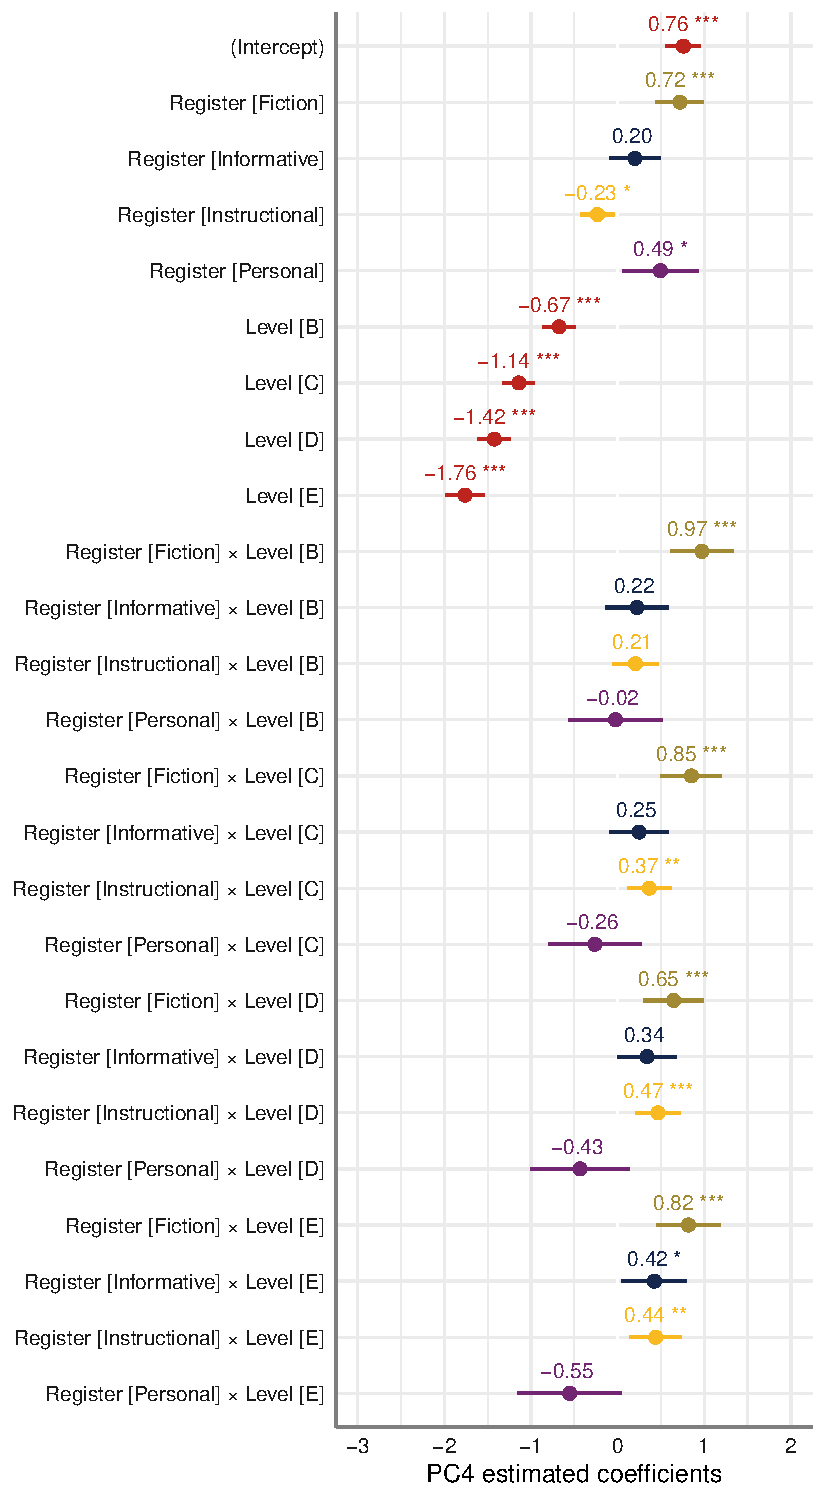
\includegraphics[keepaspectratio]{AppendixF_files/figure-pdf/Dim4model-1.pdf}}

\begin{Shaded}
\begin{Highlighting}[]
\CommentTok{\#ggsave(here("plots", "TxB\_PCA4\_lmer\_fixedeffects.svg"), height = 8, width = 8)}
\end{Highlighting}
\end{Shaded}

\begin{Shaded}
\begin{Highlighting}[]
\CommentTok{\# Plot of random effects:}
\FunctionTok{plot\_model}\NormalTok{(md4, }
           \AttributeTok{type =} \StringTok{"re"}\NormalTok{, }\CommentTok{\# Option to visualise random effects}
           \AttributeTok{show.values=}\ConstantTok{TRUE}\NormalTok{, }
           \AttributeTok{show.p=}\ConstantTok{TRUE}\NormalTok{,}
           \AttributeTok{value.offset =}\NormalTok{ .}\DecValTok{4}\NormalTok{,}
           \AttributeTok{value.size =} \FloatTok{3.5}\NormalTok{,}
           \AttributeTok{color =} \StringTok{"bw"}\NormalTok{,}
           \AttributeTok{wrap.labels =} \DecValTok{40}\NormalTok{,}
           \AttributeTok{axis.title =} \StringTok{"PC4 estimated coefficients"}\NormalTok{) }\SpecialCharTok{+}
  \FunctionTok{theme\_sjplot2}\NormalTok{()}
\end{Highlighting}
\end{Shaded}

\pandocbounded{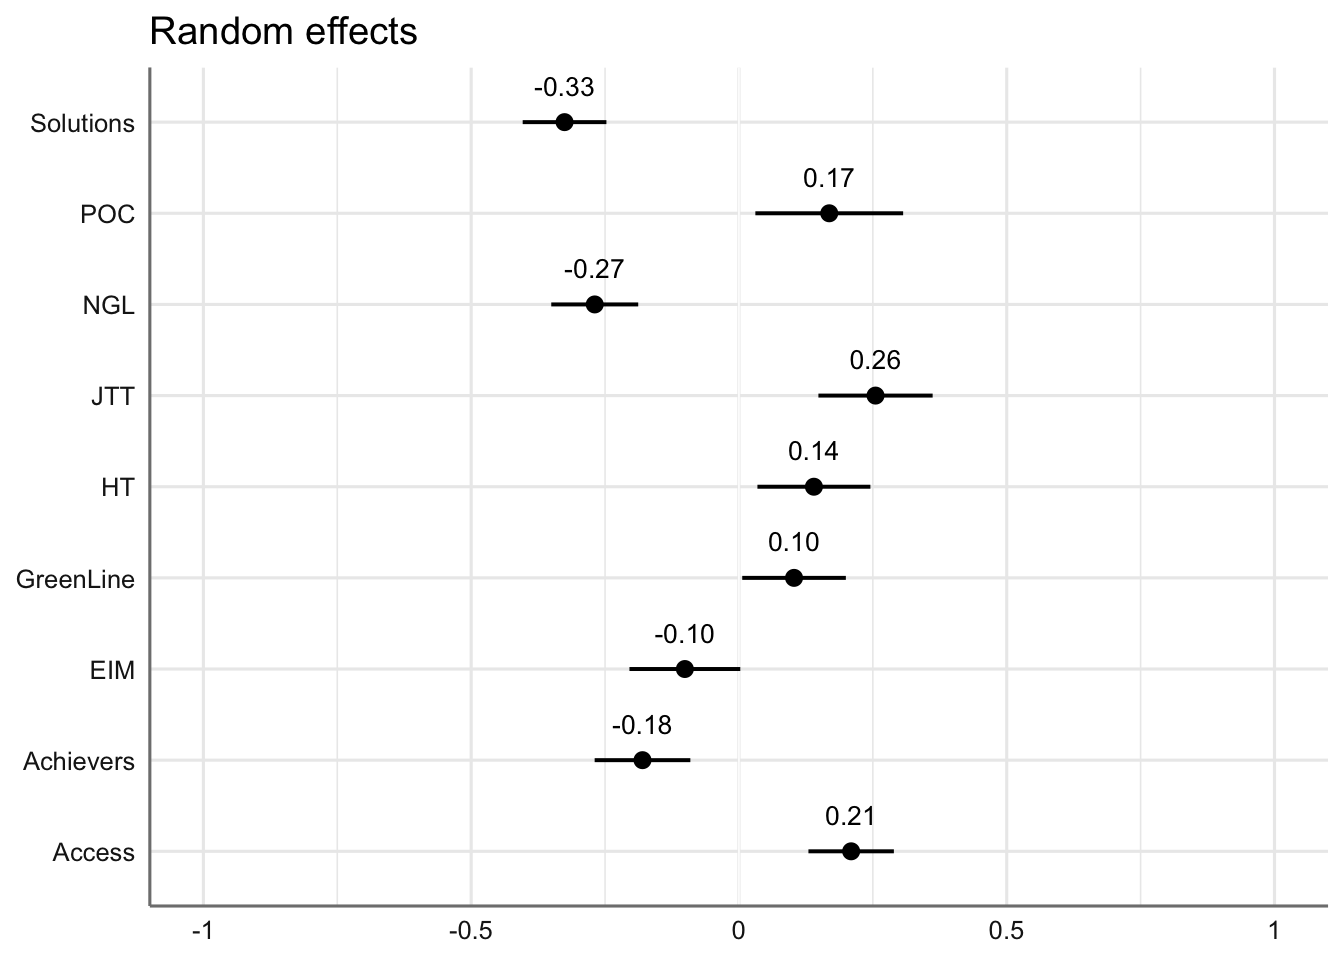
\includegraphics[keepaspectratio]{AppendixF_files/figure-pdf/unnamed-chunk-37-1.pdf}}

\begin{Shaded}
\begin{Highlighting}[]
\CommentTok{\#ggsave(here("plots", "TxB\_PCA4\_lmer\_randomeffects.svg"), height = 3, width = 8)}
\end{Highlighting}
\end{Shaded}

\begin{Shaded}
\begin{Highlighting}[]
\CommentTok{\# svg(here("plots", "TxB\_predicted\_PC4\_scores\_interactions.svg"), height = 5, width = 8)}
\FunctionTok{visreg}\NormalTok{(md4, }\AttributeTok{xvar =} \StringTok{"Level"}\NormalTok{, }\AttributeTok{by=}\StringTok{"Register"}\NormalTok{, }\AttributeTok{type =} \StringTok{"conditional"}\NormalTok{,}
       \AttributeTok{line=}\FunctionTok{list}\NormalTok{(}\AttributeTok{col=}\StringTok{"darkred"}\NormalTok{), }
       \AttributeTok{xlab =} \StringTok{"Textbook Level"}\NormalTok{, }\AttributeTok{ylab =} \StringTok{"PC4"}
       \CommentTok{\#,gg = TRUE}
\NormalTok{       ,}\AttributeTok{layout=}\FunctionTok{c}\NormalTok{(}\DecValTok{5}\NormalTok{,}\DecValTok{1}\NormalTok{)}
\NormalTok{)}
\end{Highlighting}
\end{Shaded}

\pandocbounded{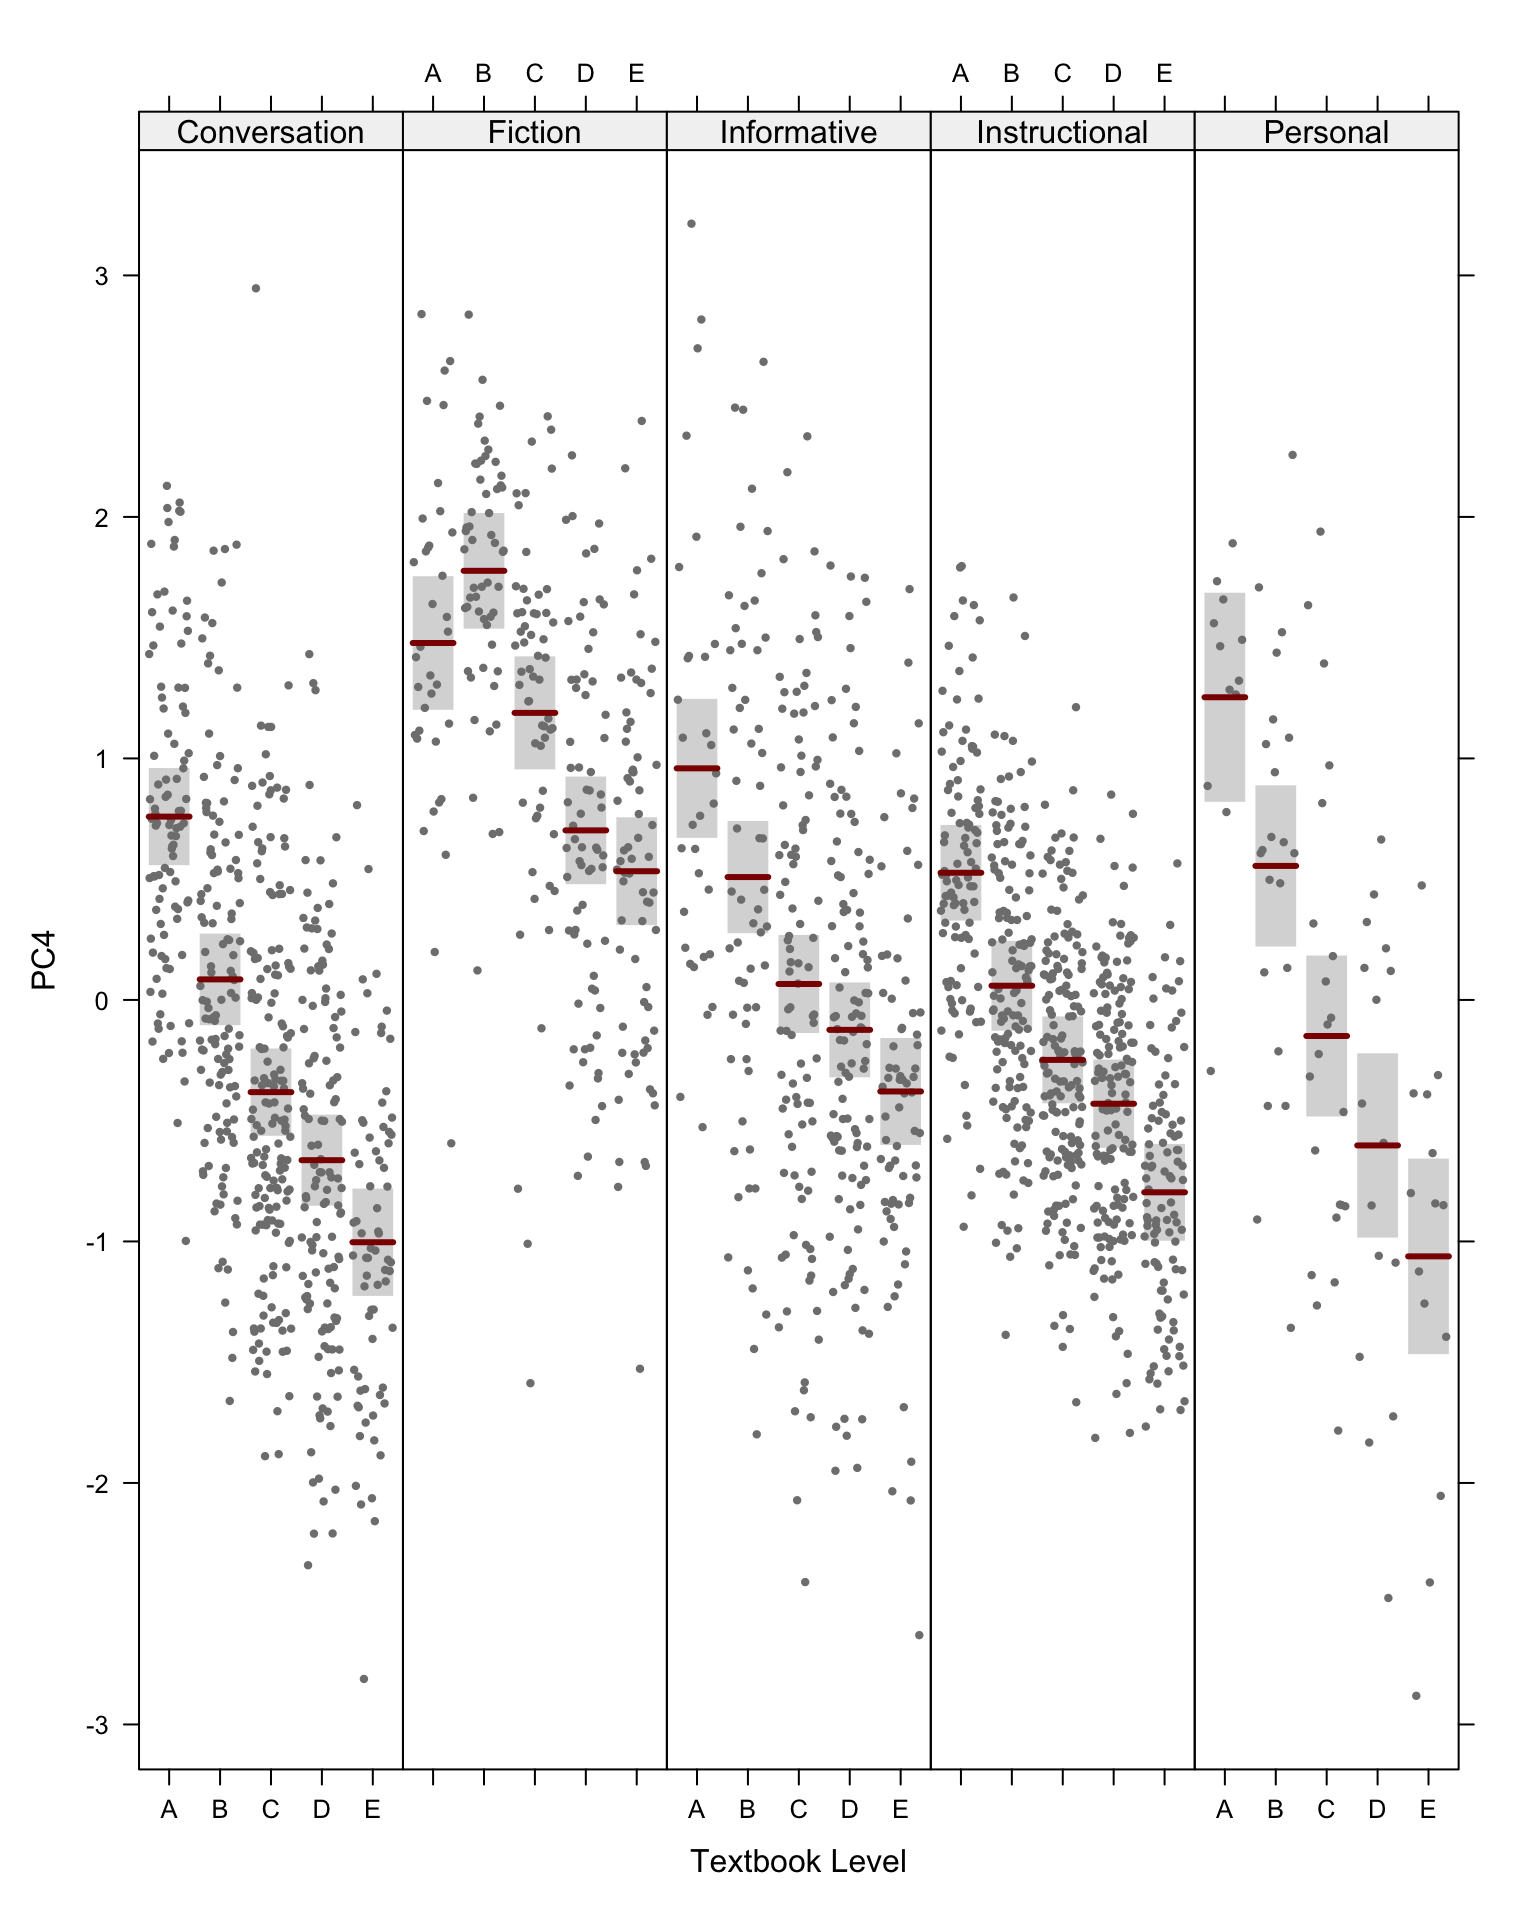
\includegraphics[keepaspectratio]{AppendixF_files/figure-pdf/unnamed-chunk-38-1.pdf}}

\begin{Shaded}
\begin{Highlighting}[]
\CommentTok{\# dev.off()}
\end{Highlighting}
\end{Shaded}

\subsection{Testing model assumptions}\label{testing-model-assumptions}

This chunk can be used to check the assumptions of all of the models
computed above. In the following example, we examine the final model
selected to predict Dim2 scores.

\begin{Shaded}
\begin{Highlighting}[]
\NormalTok{model2test }\OtherTok{\textless{}{-}}\NormalTok{ md2}

\CommentTok{\# check distribution of residuals}
\FunctionTok{plot}\NormalTok{(model2test)}
\end{Highlighting}
\end{Shaded}

\pandocbounded{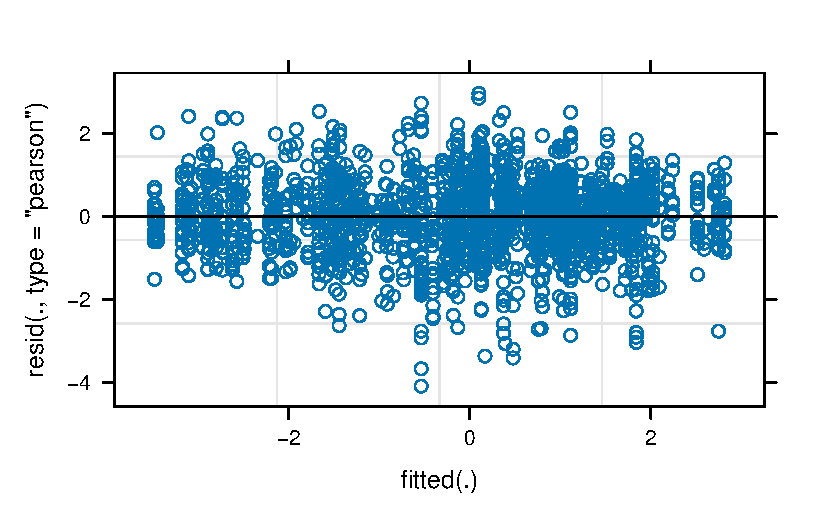
\includegraphics[keepaspectratio]{AppendixF_files/figure-pdf/lmer-diagnostics-1.pdf}}

\begin{Shaded}
\begin{Highlighting}[]
\CommentTok{\# scale{-}location plot}
\FunctionTok{plot}\NormalTok{(model2test,}
     \FunctionTok{sqrt}\NormalTok{(}\FunctionTok{abs}\NormalTok{(}\FunctionTok{resid}\NormalTok{(.)))}\SpecialCharTok{\textasciitilde{}}\FunctionTok{fitted}\NormalTok{(.),}
     \AttributeTok{type=}\FunctionTok{c}\NormalTok{(}\StringTok{"p"}\NormalTok{,}\StringTok{"smooth"}\NormalTok{), }\AttributeTok{col.line=}\DecValTok{1}\NormalTok{)}
\end{Highlighting}
\end{Shaded}

\pandocbounded{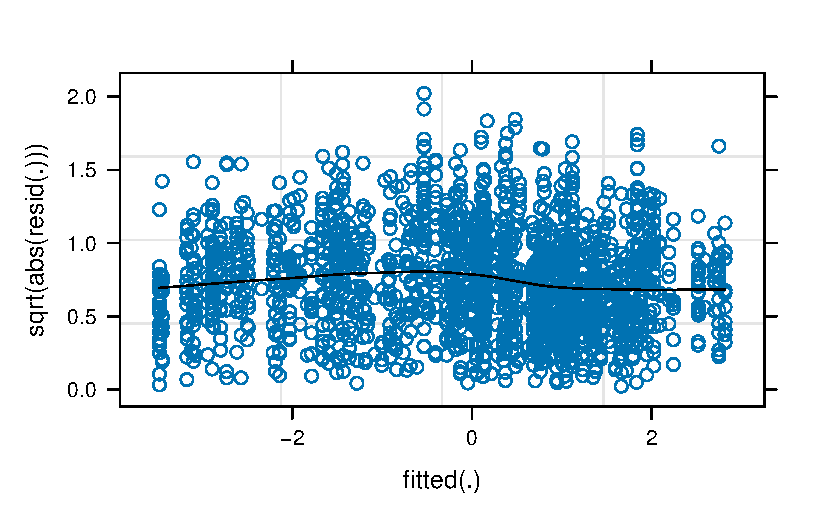
\includegraphics[keepaspectratio]{AppendixF_files/figure-pdf/lmer-diagnostics-2.pdf}}

\begin{Shaded}
\begin{Highlighting}[]
\CommentTok{\# Q{-}Q plot}
\NormalTok{lattice}\SpecialCharTok{::}\FunctionTok{qqmath}\NormalTok{(model2test)}
\end{Highlighting}
\end{Shaded}

\pandocbounded{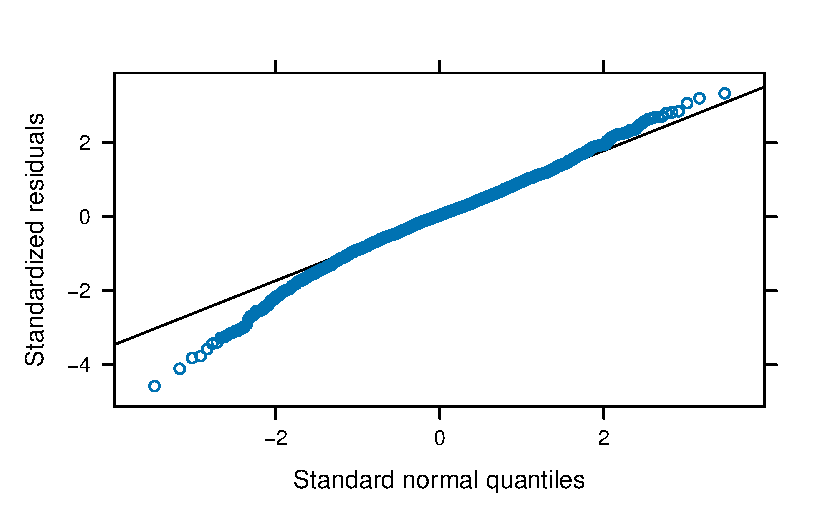
\includegraphics[keepaspectratio]{AppendixF_files/figure-pdf/lmer-diagnostics-3.pdf}}

\section{Packages used in this
script}\label{packages-used-in-this-script-2}

\subsection{Package names and
versions}\label{package-names-and-versions-2}

\begin{verbatim}
R version 4.4.1 (2024-06-14)
Platform: aarch64-apple-darwin20
Running under: macOS Sonoma 14.5

Matrix products: default
BLAS:   /Library/Frameworks/R.framework/Versions/4.4-arm64/Resources/lib/libRblas.0.dylib 
LAPACK: /Library/Frameworks/R.framework/Versions/4.4-arm64/Resources/lib/libRlapack.dylib;  LAPACK version 3.12.0

locale:
[1] en_US.UTF-8/en_US.UTF-8/en_US.UTF-8/C/en_US.UTF-8/en_US.UTF-8

time zone: Europe/Madrid
tzcode source: internal

attached base packages:
[1] stats     graphics  grDevices datasets  utils     methods   base     

other attached packages:
 [1] visreg_2.7.0      lubridate_1.9.3   stringr_1.5.1     dplyr_1.1.4      
 [5] purrr_1.0.2       readr_2.1.5       tidyr_1.3.1       tibble_3.2.1     
 [9] tidyverse_2.0.0   sjPlot_2.8.16     psych_2.4.6.26    PCAtools_2.14.0  
[13] ggrepel_0.9.5     patchwork_1.2.0   lme4_1.1-35.5     Matrix_1.7-0     
[17] knitr_1.48        here_1.0.1        ggthemes_5.1.0    forcats_1.0.0    
[21] factoextra_1.0.7  emmeans_1.10.3    DescTools_0.99.54 cowplot_1.1.3    
[25] caret_6.0-94      lattice_0.22-6    ggplot2_3.5.1    

loaded via a namespace (and not attached):
  [1] rstudioapi_0.16.0         jsonlite_1.8.8           
  [3] datawizard_0.12.1         magrittr_2.0.3           
  [5] estimability_1.5.1        nloptr_2.1.1             
  [7] rmarkdown_2.27            zlibbioc_1.50.0          
  [9] vctrs_0.6.5               minqa_1.2.7              
 [11] DelayedMatrixStats_1.26.0 htmltools_0.5.8.1        
 [13] S4Arrays_1.4.1            cellranger_1.1.0         
 [15] sjmisc_2.8.10             SparseArray_1.4.8        
 [17] pROC_1.18.5               parallelly_1.37.1        
 [19] plyr_1.8.9                rootSolve_1.8.2.4        
 [21] lifecycle_1.0.4           iterators_1.0.14         
 [23] pkgconfig_2.0.3           sjlabelled_1.2.0         
 [25] rsvd_1.0.5                R6_2.5.1                 
 [27] fastmap_1.2.0             MatrixGenerics_1.16.0    
 [29] future_1.33.2             digest_0.6.36            
 [31] Exact_3.2                 colorspace_2.1-0         
 [33] S4Vectors_0.42.1          rprojroot_2.0.4          
 [35] dqrng_0.4.1               irlba_2.3.5.1            
 [37] beachmat_2.20.0           fansi_1.0.6              
 [39] timechange_0.3.0          httr_1.4.7               
 [41] abind_1.4-5               compiler_4.4.1           
 [43] proxy_0.4-27              withr_3.0.0              
 [45] BiocParallel_1.38.0       performance_0.12.2       
 [47] MASS_7.3-60.2             lava_1.8.0               
 [49] sjstats_0.19.0            DelayedArray_0.30.1      
 [51] gld_2.6.6                 ModelMetrics_1.2.2.2     
 [53] tools_4.4.1               future.apply_1.11.2      
 [55] nnet_7.3-19               glue_1.7.0               
 [57] nlme_3.1-164              grid_4.4.1               
 [59] reshape2_1.4.4            generics_0.1.3           
 [61] recipes_1.1.0             gtable_0.3.5             
 [63] tzdb_0.4.0                class_7.3-22             
 [65] hms_1.1.3                 data.table_1.15.4        
 [67] lmom_3.0                  BiocSingular_1.20.0      
 [69] ScaledMatrix_1.12.0       utf8_1.2.4               
 [71] XVector_0.44.0            BiocGenerics_0.50.0      
 [73] foreach_1.5.2             pillar_1.9.0             
 [75] splines_4.4.1             renv_1.0.3               
 [77] survival_3.6-4            tidyselect_1.2.1         
 [79] IRanges_2.38.1            stats4_4.4.1             
 [81] xfun_0.46                 expm_0.999-9             
 [83] hardhat_1.4.0             timeDate_4032.109        
 [85] matrixStats_1.3.0         stringi_1.8.4            
 [87] yaml_2.3.9                boot_1.3-30              
 [89] evaluate_0.24.0           codetools_0.2-20         
 [91] BiocManager_1.30.23       cli_3.6.3                
 [93] rpart_4.1.23              xtable_1.8-4             
 [95] munsell_0.5.1             Rcpp_1.0.13              
 [97] readxl_1.4.3              globals_0.16.3           
 [99] ggeffects_1.7.0           coda_0.19-4.1            
[101] parallel_4.4.1            gower_1.0.1              
[103] sparseMatrixStats_1.16.0  listenv_0.9.1            
[105] mvtnorm_1.2-5             ipred_0.9-15             
[107] scales_1.3.0              prodlim_2024.06.25       
[109] e1071_1.7-14              insight_0.20.2           
[111] crayon_1.5.3              rlang_1.1.4              
[113] mnormt_2.1.1             
\end{verbatim}

\subsection{Package references}\label{package-references-2}

{[}1{]} J. B. Arnold. \emph{ggthemes: Extra Themes, Scales and Geoms for
ggplot2}. R package version 5.1.0. 2024.
\url{https://jrnold.github.io/ggthemes/}.

{[}2{]} D. Bates, M. Mächler, B. Bolker, et al.~``Fitting Linear
Mixed-Effects Models Using lme4''. In: \emph{Journal of Statistical
Software} 67.1 (2015), pp.~1-48. DOI: 10.18637/jss.v067.i01.

{[}3{]} D. Bates, M. Maechler, B. Bolker, et al.~\emph{lme4: Linear
Mixed-Effects Models using Eigen and S4}. R package version 1.1-35.5.
2024. \url{https://github.com/lme4/lme4/}.

{[}4{]} D. Bates, M. Maechler, and M. Jagan. \emph{Matrix: Sparse and
Dense Matrix Classes and Methods}. R package version 1.7-0. 2024.
\url{https://Matrix.R-forge.R-project.org}.

{[}5{]} K. Blighe and A. Lun. \emph{PCAtools: Everything Principal
Components Analysis}. R package version 2.14.0. 2023. DOI:
10.18129/B9.bioc.PCAtools.
\url{https://bioconductor.org/packages/PCAtools}.

{[}6{]} P. Breheny and W. Burchett. \emph{visreg: Visualization of
Regression Models}. R package version 2.7.0. 2020.
\url{http://pbreheny.github.io/visreg}.

{[}7{]} P. Breheny and W. Burchett. ``Visualization of Regression Models
Using visreg''. In: \emph{The R Journal} 9.2 (2017), pp.~56-71.

{[}8{]} G. Grolemund and H. Wickham. ``Dates and Times Made Easy with
lubridate''. In: \emph{Journal of Statistical Software} 40.3 (2011), pp.
1-25. \url{https://www.jstatsoft.org/v40/i03/}.

{[}9{]} A. Kassambara and F. Mundt. \emph{factoextra: Extract and
Visualize the Results of Multivariate Data Analyses}. R package version
1.0.7. 2020. \url{http://www.sthda.com/english/rpkgs/factoextra}.

{[}10{]} M. Kuhn. \emph{caret: Classification and Regression Training}.
R package version 6.0-94. 2023. \url{https://github.com/topepo/caret/}.

{[}11{]} Kuhn and Max. ``Building Predictive Models in R Using the caret
Package''. In: \emph{Journal of Statistical Software} 28.5 (2008),
p.~1--26. DOI: 10.18637/jss.v028.i05.
\url{https://www.jstatsoft.org/index.php/jss/article/view/v028i05}.

{[}12{]} R. V. Lenth. \emph{emmeans: Estimated Marginal Means, aka
Least-Squares Means}. R package version 1.10.3. 2024.
\url{https://rvlenth.github.io/emmeans/}.

{[}13{]} D. Lüdecke. \emph{sjPlot: Data Visualization for Statistics in
Social Science}. R package version 2.8.16. 2024.
\url{https://strengejacke.github.io/sjPlot/}.

{[}14{]} K. Müller. \emph{here: A Simpler Way to Find Your Files}. R
package version 1.0.1. 2020. \url{https://here.r-lib.org/}.

{[}15{]} K. Müller and H. Wickham. \emph{tibble: Simple Data Frames}. R
package version 3.2.1. 2023. \url{https://tibble.tidyverse.org/}.

{[}16{]} T. L. Pedersen. \emph{patchwork: The Composer of Plots}. R
package version 1.2.0. 2024. \url{https://patchwork.data-imaginist.com}.

{[}17{]} R Core Team. \emph{R: A Language and Environment for
Statistical Computing}. R Foundation for Statistical Computing. Vienna,
Austria, 2024. \url{https://www.R-project.org/}.

{[}18{]} W. Revelle. \emph{psych: Procedures for Psychological,
Psychometric, and Personality Research}. R package version 2.4.6.26.
2024. \url{https://personality-project.org/r/psych/}.

{[}19{]} D. Sarkar. \emph{Lattice: Multivariate Data Visualization with
R}. New York: Springer, 2008. ISBN: 978-0-387-75968-5.
\url{http://lmdvr.r-forge.r-project.org}.

{[}20{]} D. Sarkar. \emph{lattice: Trellis Graphics for R}. R package
version 0.22-6. 2024. \url{https://lattice.r-forge.r-project.org/}.

{[}21{]} A. Signorell. \emph{DescTools: Tools for Descriptive
Statistics}. R package version 0.99.54. 2024.
\url{https://andrisignorell.github.io/DescTools/}.

{[}22{]} K. Slowikowski. \emph{ggrepel: Automatically Position
Non-Overlapping Text Labels with ggplot2}. R package version 0.9.5.
2024. \url{https://ggrepel.slowkow.com/}.

{[}23{]} V. Spinu, G. Grolemund, and H. Wickham. \emph{lubridate: Make
Dealing with Dates a Little Easier}. R package version 1.9.3. 2023.
\url{https://lubridate.tidyverse.org}.

{[}24{]} H. Wickham. \emph{forcats: Tools for Working with Categorical
Variables (Factors)}. R package version 1.0.0. 2023.
\url{https://forcats.tidyverse.org/}.

{[}25{]} H. Wickham. \emph{ggplot2: Elegant Graphics for Data Analysis}.
Springer-Verlag New York, 2016. ISBN: 978-3-319-24277-4.
\url{https://ggplot2.tidyverse.org}.

{[}26{]} H. Wickham. \emph{stringr: Simple, Consistent Wrappers for
Common String Operations}. R package version 1.5.1. 2023.
\url{https://stringr.tidyverse.org}.

{[}27{]} H. Wickham. \emph{tidyverse: Easily Install and Load the
Tidyverse}. R package version 2.0.0. 2023.
\url{https://tidyverse.tidyverse.org}.

{[}28{]} H. Wickham, M. Averick, J. Bryan, et al.~``Welcome to the
tidyverse''. In: \emph{Journal of Open Source Software} 4.43 (2019),
p.~1686. DOI: 10.21105/joss.01686.

{[}29{]} H. Wickham, W. Chang, L. Henry, et al.~\emph{ggplot2: Create
Elegant Data Visualisations Using the Grammar of Graphics}. R package
version 3.5.1. 2024. \url{https://ggplot2.tidyverse.org}.

{[}30{]} H. Wickham, R. François, L. Henry, et al.~\emph{dplyr: A
Grammar of Data Manipulation}. R package version 1.1.4. 2023.
\url{https://dplyr.tidyverse.org}.

{[}31{]} H. Wickham and L. Henry. \emph{purrr: Functional Programming
Tools}. R package version 1.0.2. 2023.
\url{https://purrr.tidyverse.org/}.

{[}32{]} H. Wickham, J. Hester, and J. Bryan. \emph{readr: Read
Rectangular Text Data}. R package version 2.1.5. 2024.
\url{https://readr.tidyverse.org}.

{[}33{]} H. Wickham, D. Vaughan, and M. Girlich. \emph{tidyr: Tidy Messy
Data}. R package version 1.3.1. 2024. \url{https://tidyr.tidyverse.org}.

{[}34{]} C. O. Wilke. \emph{cowplot: Streamlined Plot Theme and Plot
Annotations for ggplot2}. R package version 1.1.3. 2024.
\url{https://wilkelab.org/cowplot/}.

{[}35{]} Y. Xie. \emph{Dynamic Documents with R and knitr}. 2nd. ISBN
978-1498716963. Boca Raton, Florida: Chapman and Hall/CRC, 2015.
\url{https://yihui.org/knitr/}.

{[}36{]} Y. Xie. ``knitr: A Comprehensive Tool for Reproducible Research
in R''. In: \emph{Implementing Reproducible Computational Research}. Ed.
by V. Stodden, F. Leisch and R. D. Peng. ISBN 978-1466561595. Chapman
and Hall/CRC, 2014.

{[}37{]} Y. Xie. \emph{knitr: A General-Purpose Package for Dynamic
Report Generation in R}. R package version 1.48. 2024.
\url{https://yihui.org/knitr/}.

\chapter{Data Preparation for the Model of Textbook English
vs.~`real-world'
English}\label{data-preparation-for-the-model-of-textbook-english-vs.-real-world-english}

This script documents the steps taken to pre-process the data extracted
from the Textbook English Corpus (TEC) and the three reference corpora
that were ultimately entered in the comparative multi-dimensional model
of Textbook English as compared to English outside the EFL classroom
(Chapter 7).

\section{Packages required}\label{packages-required-2}

The following packages must be installed and loaded to process the data.

\begin{Shaded}
\begin{Highlighting}[]
\CommentTok{\#renv::restore() \# Restore the project\textquotesingle{}s dependencies from the lockfile to ensure that same package versions are used as in the original thesis.}

\FunctionTok{library}\NormalTok{(broom.mixed) }\CommentTok{\# For checking singularity issues }
\FunctionTok{library}\NormalTok{(car) }\CommentTok{\# For recoding data}
\FunctionTok{library}\NormalTok{(corrplot) }\CommentTok{\# For the feature correlation matrix}
\FunctionTok{library}\NormalTok{(cowplot) }\CommentTok{\# For nice plots}
\FunctionTok{library}\NormalTok{(DT) }\CommentTok{\# To display interactive HTML tables}
\FunctionTok{library}\NormalTok{(emmeans) }\CommentTok{\# Comparing group means of predicted values}
\FunctionTok{library}\NormalTok{(GGally) }\CommentTok{\# For ggpairs}
\FunctionTok{library}\NormalTok{(gridExtra) }\CommentTok{\# For making large faceted plots}
\FunctionTok{library}\NormalTok{(here) }\CommentTok{\# For ease of sharing}
\FunctionTok{library}\NormalTok{(knitr) }\CommentTok{\# Loaded to display the tables using the kable() function}
\FunctionTok{library}\NormalTok{(lme4) }\CommentTok{\# For mixed effects modelling}
\FunctionTok{library}\NormalTok{(psych) }\CommentTok{\# For various useful stats function, including KMO()}
\FunctionTok{library}\NormalTok{(scales) }\CommentTok{\# For working with colours}
\FunctionTok{library}\NormalTok{(sjPlot) }\CommentTok{\# For nice tabular display of regression models}
\FunctionTok{library}\NormalTok{(tidyverse) }\CommentTok{\# For data wrangling and plotting}
\FunctionTok{library}\NormalTok{(visreg) }\CommentTok{\# For nice visualisations of model results}
\NormalTok{select }\OtherTok{\textless{}{-}}\NormalTok{ dplyr}\SpecialCharTok{::}\NormalTok{select}
\NormalTok{filter }\OtherTok{\textless{}{-}}\NormalTok{ dplyr}\SpecialCharTok{::}\NormalTok{filter}
\end{Highlighting}
\end{Shaded}

\section{Data import from MFTE
outputs}\label{data-import-from-mfte-outputs}

The raw data used in this script comes from the matrices of mixed
normalised frequencies as output by the
\href{https://github.com/mshakirDr/MultiFeatureTaggerEnglish}{MFTE Perl
v. 3.1} (Le Foll 2021b).

\subsection{Spoken BNC2014}\label{spoken-bnc2014-1}

\begin{Shaded}
\begin{Highlighting}[]
\NormalTok{SpokenBNC2014 }\OtherTok{\textless{}{-}} \FunctionTok{read.delim}\NormalTok{(}\FunctionTok{here}\NormalTok{(}\StringTok{"data"}\NormalTok{, }\StringTok{"MFTE"}\NormalTok{, }\StringTok{"SpokenBNC2014\_3.1\_normed\_complex\_counts.tsv"}\NormalTok{), }\AttributeTok{header =} \ConstantTok{TRUE}\NormalTok{, }\AttributeTok{stringsAsFactors =} \ConstantTok{TRUE}\NormalTok{)}

\NormalTok{SpokenBNC2014}\SpecialCharTok{$}\NormalTok{Series }\OtherTok{\textless{}{-}} \StringTok{"Spoken BNC2014"}
\NormalTok{SpokenBNC2014}\SpecialCharTok{$}\NormalTok{Level }\OtherTok{\textless{}{-}} \StringTok{"Ref."}
\NormalTok{SpokenBNC2014}\SpecialCharTok{$}\NormalTok{Country }\OtherTok{\textless{}{-}} \StringTok{"Spoken BNC2014"}
\NormalTok{SpokenBNC2014}\SpecialCharTok{$}\NormalTok{Register }\OtherTok{\textless{}{-}} \StringTok{"Spoken BNC2014"}
\end{Highlighting}
\end{Shaded}

These normalised frequencies were computed on the basis of my own ``John
and Jill in Ivybridge'' version of the Spoken BNC2014 with added full
stops at speaker turns (see Appendix B for details). This corpus
comprises of 1,251 texts, all of which were used in the following
analyses.

\pandocbounded{
\includegraphics[keepaspectratio]{AppendixG_files/figure-pdf/unnamed-chunk-2-1.pdf}}

\subsection{Youth Fiction corpus}\label{youth-fiction-corpus-1}

\begin{Shaded}
\begin{Highlighting}[]
\NormalTok{YouthFiction }\OtherTok{\textless{}{-}} \FunctionTok{read.delim}\NormalTok{(}\FunctionTok{here}\NormalTok{(}\StringTok{"data"}\NormalTok{, }\StringTok{"MFTE"}\NormalTok{, }\StringTok{"YF\_sampled\_500\_3.1\_normed\_complex\_counts.tsv"}\NormalTok{), }\AttributeTok{header =} \ConstantTok{TRUE}\NormalTok{, }\AttributeTok{stringsAsFactors =} \ConstantTok{TRUE}\NormalTok{)}

\NormalTok{YouthFiction}\SpecialCharTok{$}\NormalTok{Series }\OtherTok{\textless{}{-}} \StringTok{"Youth Fiction"}
\NormalTok{YouthFiction}\SpecialCharTok{$}\NormalTok{Level }\OtherTok{\textless{}{-}} \StringTok{"Ref."}
\NormalTok{YouthFiction}\SpecialCharTok{$}\NormalTok{Country }\OtherTok{\textless{}{-}} \StringTok{"Youth Fiction"}
\NormalTok{YouthFiction}\SpecialCharTok{$}\NormalTok{Register }\OtherTok{\textless{}{-}} \StringTok{"Youth Fiction"}
\end{Highlighting}
\end{Shaded}

These normalised frequencies were computed on the basis of the random
samples of approximately 5,000 words of the books of the Youth Fiction
corpus (for details of the works included in this corpus, see Appendix
B). The sampling procedure is described in Section 4.3.2.4 of the book.
This dataset consists of 1,191 files.

\pandocbounded{
\includegraphics[keepaspectratio]{AppendixG_files/figure-pdf/unnamed-chunk-3-1.pdf}}

\subsection{Informative Texts for Teens (InfoTeens)
corpus}\label{informative-texts-for-teens-infoteens-corpus}

\begin{Shaded}
\begin{Highlighting}[]
\NormalTok{InfoTeen }\OtherTok{\textless{}{-}} \FunctionTok{read.delim}\NormalTok{(}\FunctionTok{here}\NormalTok{(}\StringTok{"data"}\NormalTok{, }\StringTok{"MFTE"}\NormalTok{, }\StringTok{"InfoTeen\_3.1\_normed\_complex\_counts.tsv"}\NormalTok{), }\AttributeTok{header =} \ConstantTok{TRUE}\NormalTok{, }\AttributeTok{stringsAsFactors =} \ConstantTok{TRUE}\NormalTok{)}

\CommentTok{\# Removes three outlier files which should not have been included in the corpus as they contain exam papers only}
\NormalTok{InfoTeen }\OtherTok{\textless{}{-}}\NormalTok{ InfoTeen }\SpecialCharTok{|\textgreater{}} 
  \FunctionTok{filter}\NormalTok{(Filename}\SpecialCharTok{!=}\StringTok{".DS\_Store"} \SpecialCharTok{\&}\NormalTok{ Filename}\SpecialCharTok{!=}\StringTok{"Revision\_World\_GCSE\_10529068\_wjec{-}level{-}law{-}past{-}papers.txt"} \SpecialCharTok{\&}\NormalTok{ Filename}\SpecialCharTok{!=}\StringTok{"Revision\_World\_GCSE\_10528474\_wjec{-}level{-}history{-}past{-}papers.txt"} \SpecialCharTok{\&}\NormalTok{ Filename}\SpecialCharTok{!=}\StringTok{"Revision\_World\_GCSE\_10528472\_edexcel{-}level{-}history{-}past{-}papers.txt"}\NormalTok{)}

\NormalTok{InfoTeen}\SpecialCharTok{$}\NormalTok{Series }\OtherTok{\textless{}{-}} \StringTok{"Info Teens"}
\NormalTok{InfoTeen}\SpecialCharTok{$}\NormalTok{Level }\OtherTok{\textless{}{-}} \StringTok{"Ref."}
\NormalTok{InfoTeen}\SpecialCharTok{$}\NormalTok{Country }\OtherTok{\textless{}{-}} \StringTok{"Info Teens"}
\NormalTok{InfoTeen}\SpecialCharTok{$}\NormalTok{Register }\OtherTok{\textless{}{-}} \StringTok{"Info Teens"}
\end{Highlighting}
\end{Shaded}

Details of the composition of the Info Teens corpus can be found in
Section 4.3.2.5 of the book. The version used in the present study
comprises 1,411 texts.

\pandocbounded{
\includegraphics[keepaspectratio]{AppendixG_files/figure-pdf/unnamed-chunk-4-1.pdf}}

\section{Merging TEC and reference corpora
data}\label{merging-tec-and-reference-corpora-data}

\subsection{Corpus size}\label{corpus-size-1}

These tables provide some summary statistics about the texts/files whose
normalised feature frequencies were entered in the model of Textbook
English vs.~real-world English described in Chapter 7.

\begin{Shaded}
\begin{Highlighting}[]
\FunctionTok{summary}\NormalTok{(ncounts}\SpecialCharTok{$}\NormalTok{Subcorpus) }\SpecialCharTok{|\textgreater{}} 
  \FunctionTok{kable}\NormalTok{(}\AttributeTok{col.names =} \FunctionTok{c}\NormalTok{(}\StringTok{"(Sub)corpus"}\NormalTok{, }\StringTok{"\# texts"}\NormalTok{),}
        \AttributeTok{format.args =} \FunctionTok{list}\NormalTok{(}\AttributeTok{big.mark =} \StringTok{","}\NormalTok{))}
\end{Highlighting}
\end{Shaded}

\begin{longtable}[]{@{}lr@{}}
\toprule\noalign{}
(Sub)corpus & \# texts \\
\midrule\noalign{}
\endhead
\bottomrule\noalign{}
\endlastfoot
Textbook Conversation & 593 \\
Textbook Fiction & 285 \\
Info Teens Ref. & 1,411 \\
Textbook Informative & 364 \\
Spoken BNC2014 Ref. & 1,251 \\
Youth Fiction Ref. & 1,191 \\
\end{longtable}

\begin{Shaded}
\begin{Highlighting}[]
\NormalTok{ncounts  }\SpecialCharTok{|\textgreater{}}  
  \FunctionTok{group\_by}\NormalTok{(Register) }\SpecialCharTok{|\textgreater{}}  
  \FunctionTok{summarise}\NormalTok{(}\AttributeTok{totaltexts =} \FunctionTok{n}\NormalTok{(), }
            \AttributeTok{totalwords =} \FunctionTok{sum}\NormalTok{(Words), }
            \AttributeTok{mean =} \FunctionTok{as.integer}\NormalTok{(}\FunctionTok{mean}\NormalTok{(Words)), }
            \AttributeTok{sd =} \FunctionTok{as.integer}\NormalTok{(}\FunctionTok{sd}\NormalTok{(Words)), }
            \AttributeTok{TTRmean =} \FunctionTok{mean}\NormalTok{(TTR)) }\SpecialCharTok{|\textgreater{}}  
  \FunctionTok{kable}\NormalTok{(}\AttributeTok{digits =} \DecValTok{2}\NormalTok{, }
        \AttributeTok{format.args =} \FunctionTok{list}\NormalTok{(}\AttributeTok{big.mark =} \StringTok{","}\NormalTok{),}
        \AttributeTok{col.names =} \FunctionTok{c}\NormalTok{(}\StringTok{"Register"}\NormalTok{, }\StringTok{"\# texts/files"}\NormalTok{, }\StringTok{"\# words"}\NormalTok{, }\StringTok{"mean \# words per text"}\NormalTok{, }\StringTok{"SD"}\NormalTok{, }\StringTok{"mean TTR"}\NormalTok{))}
\end{Highlighting}
\end{Shaded}

\begin{longtable}[]{@{}
  >{\raggedright\arraybackslash}p{(\linewidth - 10\tabcolsep) * \real{0.1733}}
  >{\raggedleft\arraybackslash}p{(\linewidth - 10\tabcolsep) * \real{0.1867}}
  >{\raggedleft\arraybackslash}p{(\linewidth - 10\tabcolsep) * \real{0.1467}}
  >{\raggedleft\arraybackslash}p{(\linewidth - 10\tabcolsep) * \real{0.2933}}
  >{\raggedleft\arraybackslash}p{(\linewidth - 10\tabcolsep) * \real{0.0800}}
  >{\raggedleft\arraybackslash}p{(\linewidth - 10\tabcolsep) * \real{0.1200}}@{}}
\toprule\noalign{}
\begin{minipage}[b]{\linewidth}\raggedright
Register
\end{minipage} & \begin{minipage}[b]{\linewidth}\raggedleft
\# texts/files
\end{minipage} & \begin{minipage}[b]{\linewidth}\raggedleft
\# words
\end{minipage} & \begin{minipage}[b]{\linewidth}\raggedleft
mean \# words per text
\end{minipage} & \begin{minipage}[b]{\linewidth}\raggedleft
SD
\end{minipage} & \begin{minipage}[b]{\linewidth}\raggedleft
mean TTR
\end{minipage} \\
\midrule\noalign{}
\endhead
\bottomrule\noalign{}
\endlastfoot
Conversation & 1,844 & 13,804,196 & 7,486 & 8,690 & 0.40 \\
Fiction & 1,476 & 7,321,747 & 4,960 & 2,022 & 0.49 \\
Informative & 1,775 & 1,436,732 & 809 & 188 & 0.51 \\
\end{longtable}

\section{Data preparation for PCA}\label{data-preparation-for-pca-1}

\subsection{Feature distributions}\label{feature-distributions-1}

The distributions of each linguistic features were examined by means of
visualisation. As shown below, before transformation, many of the
features displayed highly skewed distributions.

\begin{Shaded}
\begin{Highlighting}[]
\CommentTok{\#ncounts \textless{}{-} readRDS(here("data", "processed", "counts3Reg.rds"))}

\NormalTok{ncounts }\SpecialCharTok{|\textgreater{}}
  \FunctionTok{select}\NormalTok{(}\SpecialCharTok{{-}}\NormalTok{Words) }\SpecialCharTok{|\textgreater{}} 
  \FunctionTok{keep}\NormalTok{(is.numeric) }\SpecialCharTok{|\textgreater{}} 
  \FunctionTok{gather}\NormalTok{() }\SpecialCharTok{|\textgreater{}} \CommentTok{\# This function from tidyr converts a selection of variables into two variables: a key and a value. The key contains the names of the original variable and the value the data. This means we can then use the facet\_wrap function from ggplot2}
  \FunctionTok{ggplot}\NormalTok{(}\FunctionTok{aes}\NormalTok{(value, }\FunctionTok{after\_stat}\NormalTok{(density))) }\SpecialCharTok{+}
    \FunctionTok{theme\_bw}\NormalTok{() }\SpecialCharTok{+}
    \FunctionTok{facet\_wrap}\NormalTok{(}\SpecialCharTok{\textasciitilde{}}\NormalTok{ key, }\AttributeTok{scales =} \StringTok{"free"}\NormalTok{, }\AttributeTok{ncol =} \DecValTok{4}\NormalTok{) }\SpecialCharTok{+}
    \FunctionTok{scale\_x\_continuous}\NormalTok{(}\AttributeTok{expand=}\FunctionTok{c}\NormalTok{(}\DecValTok{0}\NormalTok{,}\DecValTok{0}\NormalTok{)) }\SpecialCharTok{+}
    \FunctionTok{scale\_y\_continuous}\NormalTok{(}\AttributeTok{limits =} \FunctionTok{c}\NormalTok{(}\DecValTok{0}\NormalTok{,}\ConstantTok{NA}\NormalTok{)) }\SpecialCharTok{+}
    \FunctionTok{geom\_histogram}\NormalTok{(}\AttributeTok{bins =} \DecValTok{30}\NormalTok{, }\AttributeTok{colour=} \StringTok{"black"}\NormalTok{, }\AttributeTok{fill =} \StringTok{"grey"}\NormalTok{) }\SpecialCharTok{+}
    \FunctionTok{geom\_density}\NormalTok{(}\AttributeTok{colour =} \StringTok{"darkred"}\NormalTok{, }\AttributeTok{weight =} \DecValTok{2}\NormalTok{, }\AttributeTok{fill=}\StringTok{"darkred"}\NormalTok{, }\AttributeTok{alpha =}\NormalTok{ .}\DecValTok{4}\NormalTok{)}
\end{Highlighting}
\end{Shaded}

\pandocbounded{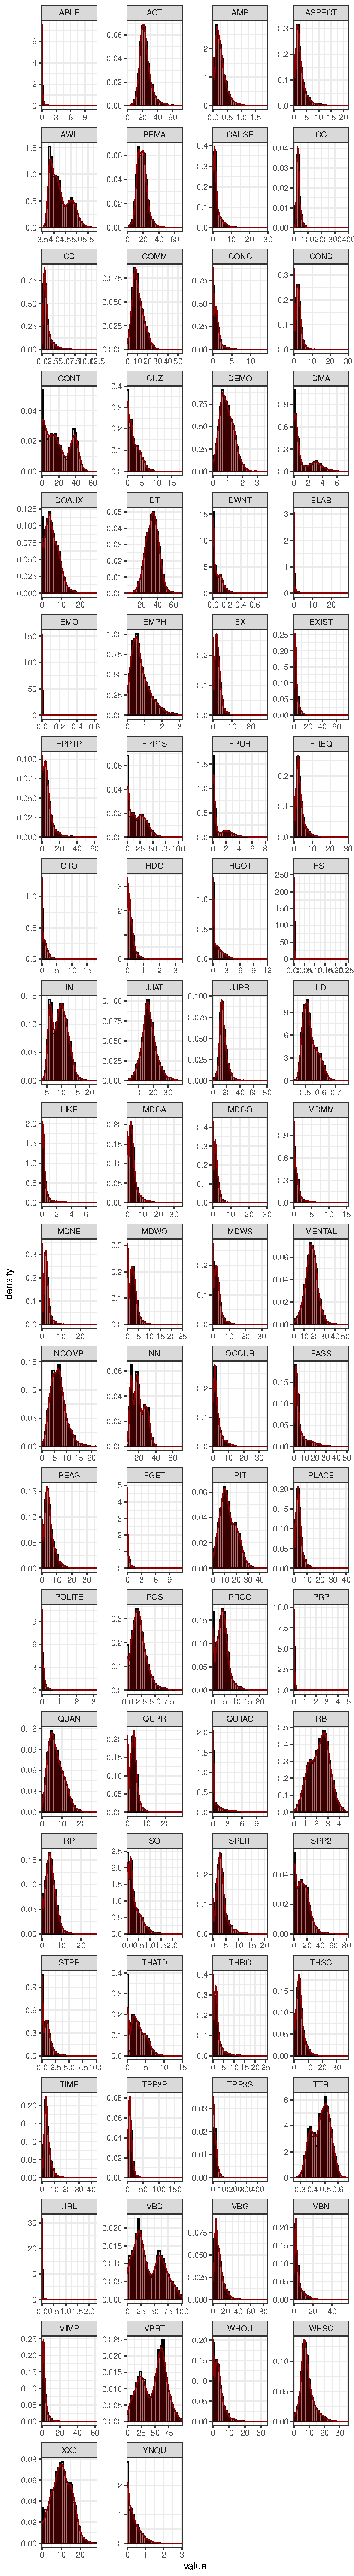
\includegraphics[keepaspectratio]{AppendixG_files/figure-pdf/distribution-viz-1.pdf}}

\begin{Shaded}
\begin{Highlighting}[]
\CommentTok{\#ggsave(here("plots", "DensityPlotsAllVariables.svg"), width = 15, height = 49)}
\end{Highlighting}
\end{Shaded}

\subsection{Feature removal}\label{feature-removal-1}

A number of features were removed from the dataset as they are not
linguistically interpretable. In the case of the TEC, this included the
variable CD because numbers spelt out as digits were removed from the
textbooks before these were tagged with the MFTE. In addition, the
variables LIKE and SO because these are ``bin'' features included in the
output of the MFTE to ensure that the counts for these polysemous words
do not inflate other categories due to mistags (Le Foll 2021c).

Whenever linguistically meaningful, very low-frequency features,
features with low MSA or communalities (see chunks below) were merged.
Finally, features absent from more than third of texts were also
excluded. For the comparative analysis of TEC and the reference corpora,
the following linguistic features were excluded from the analysis due to
low dispersion:

\begin{Shaded}
\begin{Highlighting}[]
\CommentTok{\# Removal of meaningless feature: CD because numbers as digits were mostly removed from the textbooks, LIKE and SO because they are dustbin categories}
\NormalTok{ncounts }\OtherTok{\textless{}{-}}\NormalTok{ ncounts }\SpecialCharTok{|\textgreater{}} 
  \FunctionTok{select}\NormalTok{(}\SpecialCharTok{{-}}\FunctionTok{c}\NormalTok{(CD, LIKE, SO))}

\CommentTok{\# Combine problematic features into meaningful groups whenever this makes linguistic sense}
\NormalTok{ncounts }\OtherTok{\textless{}{-}}\NormalTok{ ncounts }\SpecialCharTok{|\textgreater{}} 
  \FunctionTok{mutate}\NormalTok{(}\AttributeTok{JJPR =}\NormalTok{ JJPR }\SpecialCharTok{+}\NormalTok{ ABLE, }\AttributeTok{ABLE =} \ConstantTok{NULL}\NormalTok{) }\SpecialCharTok{|\textgreater{}} 
  \FunctionTok{mutate}\NormalTok{(}\AttributeTok{PASS =}\NormalTok{ PGET }\SpecialCharTok{+}\NormalTok{ PASS, }\AttributeTok{PGET =} \ConstantTok{NULL}\NormalTok{) }\SpecialCharTok{|\textgreater{}} 
  \FunctionTok{mutate}\NormalTok{(}\AttributeTok{TPP3 =}\NormalTok{ TPP3S }\SpecialCharTok{+}\NormalTok{ TPP3P, }\AttributeTok{TPP3P =} \ConstantTok{NULL}\NormalTok{, }\AttributeTok{TPP3S =} \ConstantTok{NULL}\NormalTok{) }\SpecialCharTok{|\textgreater{}} \CommentTok{\# Merged due to TTP3P having an individual MSA \textless{} 0.5}
  \FunctionTok{mutate}\NormalTok{(}\AttributeTok{FQTI =}\NormalTok{ FREQ }\SpecialCharTok{+}\NormalTok{ TIME, }\AttributeTok{FREQ =} \ConstantTok{NULL}\NormalTok{, }\AttributeTok{TIME =} \ConstantTok{NULL}\NormalTok{) }\CommentTok{\# Merged due to TIME communality \textless{} 0.2 (see below)}

\CommentTok{\# Function to compute percentage of texts with occurrences meeting a condition}
\NormalTok{compute\_percentage }\OtherTok{\textless{}{-}} \ControlFlowTok{function}\NormalTok{(data, condition, threshold) \{}
\NormalTok{  numeric\_data }\OtherTok{\textless{}{-}} \FunctionTok{Filter}\NormalTok{(is.numeric, data)}
\NormalTok{  percentage }\OtherTok{\textless{}{-}} \FunctionTok{round}\NormalTok{(}\FunctionTok{colSums}\NormalTok{(condition[, }\FunctionTok{sapply}\NormalTok{(numeric\_data, is.numeric)])}\SpecialCharTok{/}\FunctionTok{nrow}\NormalTok{(data) }\SpecialCharTok{*} \DecValTok{100}\NormalTok{, }\DecValTok{2}\NormalTok{)}
\NormalTok{  percentage }\OtherTok{\textless{}{-}} \FunctionTok{as.data.frame}\NormalTok{(percentage)}
  \FunctionTok{colnames}\NormalTok{(percentage) }\OtherTok{\textless{}{-}} \StringTok{"Percentage"}
\NormalTok{  percentage }\OtherTok{\textless{}{-}}\NormalTok{ percentage }\SpecialCharTok{|\textgreater{}} 
    \FunctionTok{filter}\NormalTok{(}\SpecialCharTok{!}\FunctionTok{is.na}\NormalTok{(Percentage)) }\SpecialCharTok{|\textgreater{}}
    \FunctionTok{rownames\_to\_column}\NormalTok{() }\SpecialCharTok{|\textgreater{}}
    \FunctionTok{arrange}\NormalTok{(Percentage)}
  \ControlFlowTok{if}\NormalTok{ (}\SpecialCharTok{!}\FunctionTok{missing}\NormalTok{(threshold)) \{}
\NormalTok{    percentage }\OtherTok{\textless{}{-}}\NormalTok{ percentage }\SpecialCharTok{|\textgreater{}} 
      \FunctionTok{filter}\NormalTok{(Percentage }\SpecialCharTok{\textgreater{}}\NormalTok{ threshold)}
\NormalTok{  \}}
  \FunctionTok{return}\NormalTok{(percentage)}
\NormalTok{\}}

\CommentTok{\# Calculate percentage of texts with 0 occurrences of each feature}
\NormalTok{zero\_features }\OtherTok{\textless{}{-}} \FunctionTok{compute\_percentage}\NormalTok{(ncounts, ncounts }\SpecialCharTok{==} \DecValTok{0}\NormalTok{, }\FloatTok{66.6}\NormalTok{)}
\NormalTok{zero\_features }\SpecialCharTok{|\textgreater{}} 
  \FunctionTok{kable}\NormalTok{(}\AttributeTok{col.names =} \FunctionTok{c}\NormalTok{(}\StringTok{"Feature"}\NormalTok{, }\StringTok{"\% texts with zero occurrences"}\NormalTok{))}
\end{Highlighting}
\end{Shaded}

\begin{longtable}[]{@{}lr@{}}
\toprule\noalign{}
Feature & \% texts with zero occurrences \\
\midrule\noalign{}
\endhead
\bottomrule\noalign{}
\endlastfoot
PRP & 85.34 \\
URL & 93.03 \\
EMO & 98.98 \\
HST & 99.55 \\
\end{longtable}

\begin{Shaded}
\begin{Highlighting}[]
\CommentTok{\# Drop variables with low document frequency}
\NormalTok{ncounts2 }\OtherTok{\textless{}{-}} \FunctionTok{select}\NormalTok{(ncounts, }\SpecialCharTok{{-}}\FunctionTok{one\_of}\NormalTok{(zero\_features}\SpecialCharTok{$}\NormalTok{rowname))}
\end{Highlighting}
\end{Shaded}

These feature removal operations resulted in a feature set of 71
linguistic variables.

\subsection{Identifying outlier texts}\label{identifying-outlier-texts}

All normalised frequencies were normalised to identify any potential
outlier texts.

\begin{Shaded}
\begin{Highlighting}[]
\CommentTok{\# First scale the normalised counts (z{-}standardisation) to be able to compare the various features}
\NormalTok{zcounts }\OtherTok{\textless{}{-}}\NormalTok{ ncounts2 }\SpecialCharTok{|\textgreater{}}
  \FunctionTok{select}\NormalTok{(}\SpecialCharTok{{-}}\NormalTok{Words) }\SpecialCharTok{|\textgreater{}} 
  \FunctionTok{keep}\NormalTok{(is.numeric) }\SpecialCharTok{|\textgreater{}} 
  \FunctionTok{scale}\NormalTok{()}

\CommentTok{\# If necessary, remove any outliers at this stage.}
\NormalTok{data }\OtherTok{\textless{}{-}} \FunctionTok{cbind}\NormalTok{(ncounts2[,}\DecValTok{1}\SpecialCharTok{:}\DecValTok{8}\NormalTok{], }\FunctionTok{as.data.frame}\NormalTok{(zcounts))}
\NormalTok{outliers }\OtherTok{\textless{}{-}}\NormalTok{ data }\SpecialCharTok{|\textgreater{}} 
 \FunctionTok{filter}\NormalTok{(}\FunctionTok{if\_any}\NormalTok{(}\FunctionTok{where}\NormalTok{(is.numeric) }\SpecialCharTok{\&} \SpecialCharTok{!}\NormalTok{Words,  }\AttributeTok{.fns =} \ControlFlowTok{function}\NormalTok{(x)\{x }\SpecialCharTok{\textgreater{}} \DecValTok{8}\NormalTok{\}))  }\SpecialCharTok{|\textgreater{}}
  \FunctionTok{select}\NormalTok{(Filename, Corpus, Register, Words) }
\end{Highlighting}
\end{Shaded}

The following outlier texts were identified according to the above
conditions and excluded in subsequent analyses.

\begin{Shaded}
\begin{Highlighting}[]
\CommentTok{\# These are potential outlier texts :}
\NormalTok{outliers }\SpecialCharTok{|\textgreater{}} 
  \FunctionTok{kable}\NormalTok{(}\AttributeTok{col.names =} \FunctionTok{c}\NormalTok{(}\StringTok{"Filename"}\NormalTok{, }\StringTok{"Corpus"}\NormalTok{, }\StringTok{"Register"}\NormalTok{, }\StringTok{"\# words"}\NormalTok{))}
\end{Highlighting}
\end{Shaded}

\begin{longtable}[]{@{}
  >{\raggedright\arraybackslash}p{(\linewidth - 6\tabcolsep) * \real{0.7045}}
  >{\raggedright\arraybackslash}p{(\linewidth - 6\tabcolsep) * \real{0.1364}}
  >{\raggedright\arraybackslash}p{(\linewidth - 6\tabcolsep) * \real{0.0985}}
  >{\raggedleft\arraybackslash}p{(\linewidth - 6\tabcolsep) * \real{0.0606}}@{}}
\toprule\noalign{}
\begin{minipage}[b]{\linewidth}\raggedright
Filename
\end{minipage} & \begin{minipage}[b]{\linewidth}\raggedright
Corpus
\end{minipage} & \begin{minipage}[b]{\linewidth}\raggedright
Register
\end{minipage} & \begin{minipage}[b]{\linewidth}\raggedleft
\# words
\end{minipage} \\
\midrule\noalign{}
\endhead
\bottomrule\noalign{}
\endlastfoot
POC\_4e\_Spoken\_0007.txt & Textbook.English & Conversation & 750 \\
Solutions\_Elementary\_ELF\_Spoken\_0013.txt & Textbook.English &
Conversation & 931 \\
EIM\_Starter\_Informative\_0004.txt & Textbook.English & Informative &
534 \\
GreenLine\_1\_Spoken\_0003.txt & Textbook.English & Conversation &
970 \\
Access\_1\_Spoken\_0011.txt & Textbook.English & Conversation & 784 \\
Achievers\_B1\_Informative\_0003.txt & Textbook.English & Informative &
926 \\
EIM\_Starter\_Spoken\_0002.txt & Textbook.English & Conversation &
824 \\
GreenLine\_1\_Spoken\_0008.txt & Textbook.English & Conversation &
876 \\
JTT\_3\_Informative\_0003.txt & Textbook.English & Informative & 699 \\
GreenLine\_1\_Spoken\_0010.txt & Textbook.English & Conversation &
701 \\
EIM\_1\_Spoken\_0012.txt & Textbook.English & Conversation & 640 \\
NGL\_1\_Spoken\_0013.txt & Textbook.English & Conversation & 940 \\
NGL\_3\_Spoken\_0018.txt & Textbook.English & Conversation & 751 \\
Solutions\_Intermediate\_Spoken\_0029.txt & Textbook.English &
Conversation & 672 \\
NGL\_1\_Spoken\_0012.txt & Textbook.English & Conversation & 910 \\
GreenLine\_1\_Spoken\_0006.txt & Textbook.English & Conversation &
622 \\
GreenLine\_2\_Spoken\_0004.txt & Textbook.English & Conversation &
1102 \\
Access\_2\_Spoken\_0023.txt & Textbook.English & Conversation & 875 \\
HT\_4\_Informative\_0006.txt & Textbook.English & Informative & 513 \\
Solutions\_Intermediate\_Informative\_0017.txt & Textbook.English &
Informative & 816 \\
EIM\_1\_Spoken\_0013.txt & Textbook.English & Conversation & 967 \\
Solutions\_Elementary\_ELF\_Spoken\_0021.txt & Textbook.English &
Conversation & 846 \\
Solutions\_Intermediate\_Plus\_Spoken\_0022.txt & Textbook.English &
Conversation & 596 \\
Access\_2\_Spoken\_0028.txt & Textbook.English & Conversation & 813 \\
NGL\_1\_Spoken\_0005.txt & Textbook.English & Conversation & 1020 \\
Solutions\_Elementary\_ELF\_Spoken\_0016.txt & Textbook.English &
Conversation & 871 \\
Solutions\_Pre-Intermediate\_ELF\_Spoken\_0007.txt & Textbook.English &
Conversation & 630 \\
Solutions\_Intermediate\_Informative\_0013.txt & Textbook.English &
Informative & 770 \\
GreenLine\_2\_Spoken\_0003.txt & Textbook.English & Conversation &
850 \\
HT\_4\_Spoken\_0010.txt & Textbook.English & Conversation & 727 \\
Solutions\_Elementary\_Informative\_0003.txt & Textbook.English &
Informative & 1051 \\
Access\_2\_Informative\_0001.txt & Textbook.English & Informative &
655 \\
Solutions\_Elementary\_Informative\_0010.txt & Textbook.English &
Informative & 708 \\
GreenLine\_1\_Informative\_0001.txt & Textbook.English & Informative &
731 \\
Access\_2\_Spoken\_0002.txt & Textbook.English & Conversation & 572 \\
Solutions\_Intermediate\_Spoken\_0019.txt & Textbook.English &
Conversation & 1024 \\
Access\_3\_Informative\_0003.txt & Textbook.English & Informative &
1000 \\
Access\_1\_Spoken\_0019.txt & Textbook.English & Conversation & 701 \\
Access\_2\_Spoken\_0013.txt & Textbook.English & Conversation & 981 \\
Solutions\_Intermediate\_Plus\_Informative\_0014.txt & Textbook.English
& Informative & 537 \\
Revision\_World\_GCSE\_10525362\_literary-terms.txt & Informative.Teens
& Informative & 790 \\
Revision\_World\_GCSE\_10528697\_p6-physics-radioactive-materials.txt &
Informative.Teens & Informative & 1015 \\
Science\_Tech\_Kinds\_NZ\_10382383\_math.txt & Informative.Teens &
Informative & 522 \\
Science\_for\_students\_10064820\_scientists-say-metabolism.txt &
Informative.Teens & Informative & 895 \\
Science\_Tech\_Kinds\_NZ\_10382388\_recycling.txt & Informative.Teens &
Informative & 666 \\
History\_Kids\_BBC\_10404337\_go\_furthers.txt & Informative.Teens &
Informative & 620 \\
Science\_Tech\_Kinds\_NZ\_10382391\_sports.txt & Informative.Teens &
Informative & 657 \\
Teen\_Kids\_News\_10402607\_so-you-want-to-be-an-archivist.txt &
Informative.Teens & Informative & 763 \\
Science\_Tech\_Kinds\_NZ\_10382234\_biology.txt & Informative.Teens &
Informative & 843 \\
Science\_Tech\_Kinds\_NZ\_10382372\_astronomy.txt & Informative.Teens &
Informative & 900 \\
Dogo\_News\_file10060404\_banana-plant-extract-may-be-the-key-to-slower-melting-ice-cream.txt
& Informative.Teens & Informative & 611 \\
Science\_Tech\_Kinds\_NZ\_10382667\_countries.txt & Informative.Teens &
Informative & 717 \\
Quatr\_us\_file10390777\_quick-summary-geological-erashtm.txt &
Informative.Teens & Informative & 643 \\
Science\_Tech\_Kinds\_NZ\_10382873\_physics.txt & Informative.Teens &
Informative & 722 \\
Science\_Tech\_Kinds\_NZ\_10382382\_light.txt & Informative.Teens &
Informative & 639 \\
Factmonster\_10053687\_august-13.txt & Informative.Teens & Informative &
523 \\
Revision\_World\_GCSE\_10526703\_limited-companies.txt &
Informative.Teens & Informative & 714 \\
Revision\_World\_GCSE\_10529637\_transition-metals.txt &
Informative.Teens & Informative & 787 \\
Quatr\_us\_10390856\_early-african-historyhtm.txt & Informative.Teens &
Informative & 1136 \\
History\_Kids\_BBC\_10401873\_ff6\_sicilylandingss.txt &
Informative.Teens & Informative & 813 \\
Quatr\_us\_10394250\_harappan.txt & Informative.Teens & Informative &
651 \\
Ducksters\_10398301\_iraqphp.txt & Informative.Teens & Informative &
657 \\
History\_Kids\_BBC\_10403171\_death\_sakkara\_gallery\_04s.txt &
Informative.Teens & Informative & 844 \\
Revision\_World\_GCSE\_10528246\_agricultural-change.txt &
Informative.Teens & Informative & 789 \\
Revision\_World\_GCSE\_10528086\_uk-government-judiciary.txt &
Informative.Teens & Informative & 1019 \\
Revision\_World\_GCSE\_10529794\_definitions.txt & Informative.Teens &
Informative & 904 \\
Encyclopedia\_Kinds\_au\_10085347\_Nobel\_Prize\_in\_Chemistry.txt &
Informative.Teens & Informative & 598 \\
Science\_for\_students\_10064875\_questions-big-melt-earths-ice-sheets-are-under-attack.txt
& Informative.Teens & Informative & 685 \\
Teen\_Kids\_News\_10403301\_golden-globe-winners-2019-the-complete-list.txt
& Informative.Teens & Informative & 800 \\
Science\_Tech\_Kinds\_NZ\_10382201\_projects.txt & Informative.Teens &
Informative & 947 \\
Revision\_World\_GCSE\_10529753\_probability.txt & Informative.Teens &
Informative & 816 \\
Encyclopedia\_Kinds\_au\_10085531\_Complex\_analysis.txt &
Informative.Teens & Informative & 735 \\
History\_Kids\_BBC\_10401890\_ff7\_ddays.txt & Informative.Teens &
Informative & 759 \\
History\_Kids\_BBC\_10403434s.txt & Informative.Teens & Informative &
732 \\
History\_Kids\_BBC\_10401872\_ff6\_italys.txt & Informative.Teens &
Informative & 786 \\
Science\_Tech\_Kinds\_NZ\_10382371\_amazing.txt & Informative.Teens &
Informative & 629 \\
Quatr\_us\_10391129\_athabascan.txt & Informative.Teens & Informative &
637 \\
Encyclopedia\_Kinds\_au\_10085355\_20th\_century.txt & Informative.Teens
& Informative & 864 \\
Dogo\_News\_10060755\_luxury-space-hotel-promises-guests-a-truly-out-of-this-world-vacation.txt
& Informative.Teens & Informative & 722 \\
Revision\_World\_GCSE\_10528072\_nationalism-practice.txt &
Informative.Teens & Informative & 776 \\
Quatr\_us\_10390861\_quatr-us-privacy-policyhtm.txt & Informative.Teens
& Informative & 960 \\
History\_Kids\_BBC\_10401909\_ff7\_bulges.txt & Informative.Teens &
Informative & 732 \\
History\_kids\_10381259\_timeline-of-mesopotamia.txt & Informative.Teens
& Informative & 768 \\
Revision\_World\_GCSE\_10528123\_gender-written-textual-analysis-framework.txt
& Informative.Teens & Informative & 905 \\
Science\_Tech\_Kinds\_NZ\_10386406\_floods.txt & Informative.Teens &
Informative & 580 \\
Revision\_World\_GCSE\_10529693\_advantages.txt & Informative.Teens &
Informative & 782 \\
Science\_Tech\_Kinds\_NZ\_10382378\_geography.txt & Informative.Teens &
Informative & 761 \\
Science\_Tech\_Kinds\_NZ\_10382374\_earth.txt & Informative.Teens &
Informative & 726 \\
Science\_for\_students\_10066286\_watering-plants-wastewater-can-spread-germs.txt
& Informative.Teens & Informative & 836 \\
Science\_Tech\_Kinds\_NZ\_10382393\_water.txt & Informative.Teens &
Informative & 856 \\
World\_Dteen\_10406069\_website\_policies.txt & Informative.Teens &
Informative & 995 \\
Science\_Tech\_Kinds\_NZ\_10382384\_metals.txt & Informative.Teens &
Informative & 669 \\
Dogo\_News\_10062028\_puppy-bowl-14-promises-viewers-a-paw-some-time-on-super-bowl-sunday.txt
& Informative.Teens & Informative & 581 \\
History\_Kids\_BBC\_10404730\_go\_furthers.txt & Informative.Teens &
Informative & 611 \\
Science\_Tech\_Kinds\_NZ\_10382385\_nature.txt & Informative.Teens &
Informative & 722 \\
Science\_for\_students\_10065015\_scientists-say-dna-sequencing.txt &
Informative.Teens & Informative & 953 \\
Quatr\_us\_file10390817\_conifers-pine-trees-gymnospermshtm.txt &
Informative.Teens & Informative & 533 \\
TweenTribute\_10051509\_it-true-elephants-cant-jump.txt &
Informative.Teens & Informative & 790 \\
Revision\_World\_GCSE\_10528494\_application-software.txt &
Informative.Teens & Informative & 855 \\
Revision\_World\_GCSE\_10529581\_different-types-questions-examinations.txt
& Informative.Teens & Informative & 742 \\
Dogo\_News\_10061669\_the-chinese-city-of-chengdu-may-soon-be-home-to-multiple-moons.txt
& Informative.Teens & Informative & 614 \\
Ducksters\_10398306\_geography\_of\_ancient\_chinaphp.txt &
Informative.Teens & Informative & 638 \\
Science\_for\_students\_10065144\_scientists-say-multiverse.txt &
Informative.Teens & Informative & 712 \\
Science\_Tech\_Kinds\_NZ\_10382211\_images.txt & Informative.Teens &
Informative & 793 \\
Factmonster\_10053754\_may-18.txt & Informative.Teens & Informative &
497 \\
World\_Dteen\_10406047\_AboutWORLDteen.txt & Informative.Teens &
Informative & 1053 \\
Ducksters\_10398078\_first\_new\_dealphp.txt & Informative.Teens &
Informative & 649 \\
Revision\_World\_GCSE\_10526926\_economies-scale.txt & Informative.Teens
& Informative & 621 \\
Factmonster\_10053201\_september-03.txt & Informative.Teens &
Informative & 445 \\
Science\_Tech\_Kinds\_NZ\_10387183\_calciumcarbonates.txt &
Informative.Teens & Informative & 804 \\
Science\_Tech\_Kinds\_NZ\_10382380\_health.txt & Informative.Teens &
Informative & 694 \\
Revision\_World\_GCSE\_10529587\_sources-finance.txt & Informative.Teens
& Informative & 665 \\
Quatr\_us\_10393444\_fishing.txt & Informative.Teens & Informative &
656 \\
Ducksters\_10398315\_glossary\_and\_termsphp.txt & Informative.Teens &
Informative & 684 \\
S5AA.txt & Spoken.BNC2014 & Conversation & 1869 \\
\end{longtable}

We check that that outlier texts are not particularly long or short
texts by looking at the distribution of text/file length of the
outliers.

\begin{Shaded}
\begin{Highlighting}[]
\FunctionTok{summary}\NormalTok{(outliers}\SpecialCharTok{$}\NormalTok{Words)}
\end{Highlighting}
\end{Shaded}

\begin{verbatim}
   Min. 1st Qu.  Median    Mean 3rd Qu.    Max. 
  445.0   655.5   751.0   773.6   860.0  1869.0 
\end{verbatim}

\begin{Shaded}
\begin{Highlighting}[]
\FunctionTok{hist}\NormalTok{(outliers}\SpecialCharTok{$}\NormalTok{Words, }\AttributeTok{breaks =} \DecValTok{30}\NormalTok{)}
\end{Highlighting}
\end{Shaded}

\pandocbounded{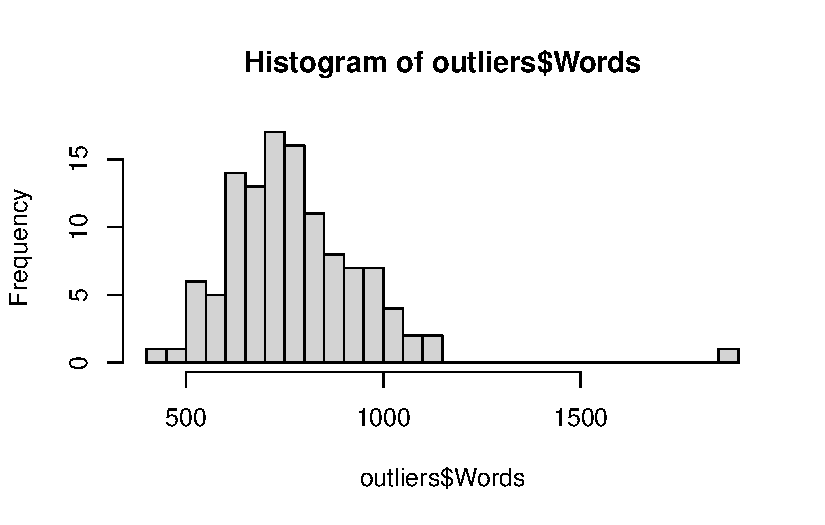
\includegraphics[keepaspectratio]{AppendixG_files/figure-pdf/unnamed-chunk-10-1.pdf}}

We also check the distribution of outlier texts across the four corpora.
The majority come from the Info Teens corpus, though quite a few are
also from the TEC.

\begin{Shaded}
\begin{Highlighting}[]
\FunctionTok{summary}\NormalTok{(outliers}\SpecialCharTok{$}\NormalTok{Corpus) }\SpecialCharTok{|\textgreater{}} 
  \FunctionTok{kable}\NormalTok{(}\AttributeTok{col.names =} \FunctionTok{c}\NormalTok{(}\StringTok{"(Sub)corpus"}\NormalTok{, }\StringTok{"\# outlier texts"}\NormalTok{))}
\end{Highlighting}
\end{Shaded}

\begin{longtable}[]{@{}lr@{}}
\toprule\noalign{}
(Sub)corpus & \# outlier texts \\
\midrule\noalign{}
\endhead
\bottomrule\noalign{}
\endlastfoot
Textbook.English & 40 \\
Informative.Teens & 74 \\
Spoken.BNC2014 & 1 \\
Youth.Fiction & 0 \\
\end{longtable}

\begin{Shaded}
\begin{Highlighting}[]
\CommentTok{\# Report on the manual check of a sample of these outliers:}

\CommentTok{\# Encyclopedia\_Kinds\_au\_10085347\_Nobel\_Prize\_in\_Chemistry.txt is essentially a list of Nobel prize winners but with some additional information. In other words, not a bad representative of the type of texts of the Info Teen corpus.}
\CommentTok{\# Solutions\_Elementary\_ELF\_Spoken\_0013 {-}{-}\textgreater{} Has a lot of "going to" constructions because they are learnt in this chapter but is otherwise a well{-}formed text.}
\CommentTok{\# Teen\_Kids\_News\_10403972\_a{-}brief{-}history{-}of{-}white{-}house{-}weddings {-}{-}\textgreater{} No issues}
\CommentTok{\# Teen\_Kids\_News\_10403301\_golden{-}globe{-}winners{-}2019{-}the{-}complete{-}list {-}{-}\textgreater{} Similar to the Nobel prize laureates text.}
\CommentTok{\# Revision\_World\_GCSE\_10528123\_gender{-}written{-}textual{-}analysis{-}framework {-}{-}\textgreater{} Text includes bullet points tokenised as the letter "o" but otherwise a fairly typical informative text.}

\CommentTok{\# Removing the outliers at the request of the reviewers (but comparisons of models including the outliers showed that the results are very similar):}
\NormalTok{ncounts3 }\OtherTok{\textless{}{-}}\NormalTok{ ncounts2 }\SpecialCharTok{|\textgreater{}} 
  \FunctionTok{filter}\NormalTok{(}\SpecialCharTok{!}\NormalTok{Filename }\SpecialCharTok{\%in\%}\NormalTok{ outliers}\SpecialCharTok{$}\NormalTok{Filename)}

\CommentTok{\#saveRDS(ncounts3, here("data", "processed", "ncounts3\_3Reg.rds")) \# Last saved 6 March 2024}
\end{Highlighting}
\end{Shaded}

This resulted in 4,980 texts/files being included in the comparative
model of Textbook English vs.~`real-world' English. These standardised
feature frequencies were distributed as follows:

\begin{Shaded}
\begin{Highlighting}[]
\NormalTok{zcounts3 }\OtherTok{\textless{}{-}}\NormalTok{ ncounts3 }\SpecialCharTok{|\textgreater{}}
  \FunctionTok{select}\NormalTok{(}\SpecialCharTok{{-}}\NormalTok{Words) }\SpecialCharTok{|\textgreater{}} 
  \FunctionTok{keep}\NormalTok{(is.numeric) }\SpecialCharTok{|\textgreater{}} 
  \FunctionTok{scale}\NormalTok{()}

\FunctionTok{boxplot}\NormalTok{(zcounts3, }\AttributeTok{las =} \DecValTok{3}\NormalTok{, }\AttributeTok{main =} \StringTok{"z{-}scores"}\NormalTok{) }\CommentTok{\# Slow}
\end{Highlighting}
\end{Shaded}

\pandocbounded{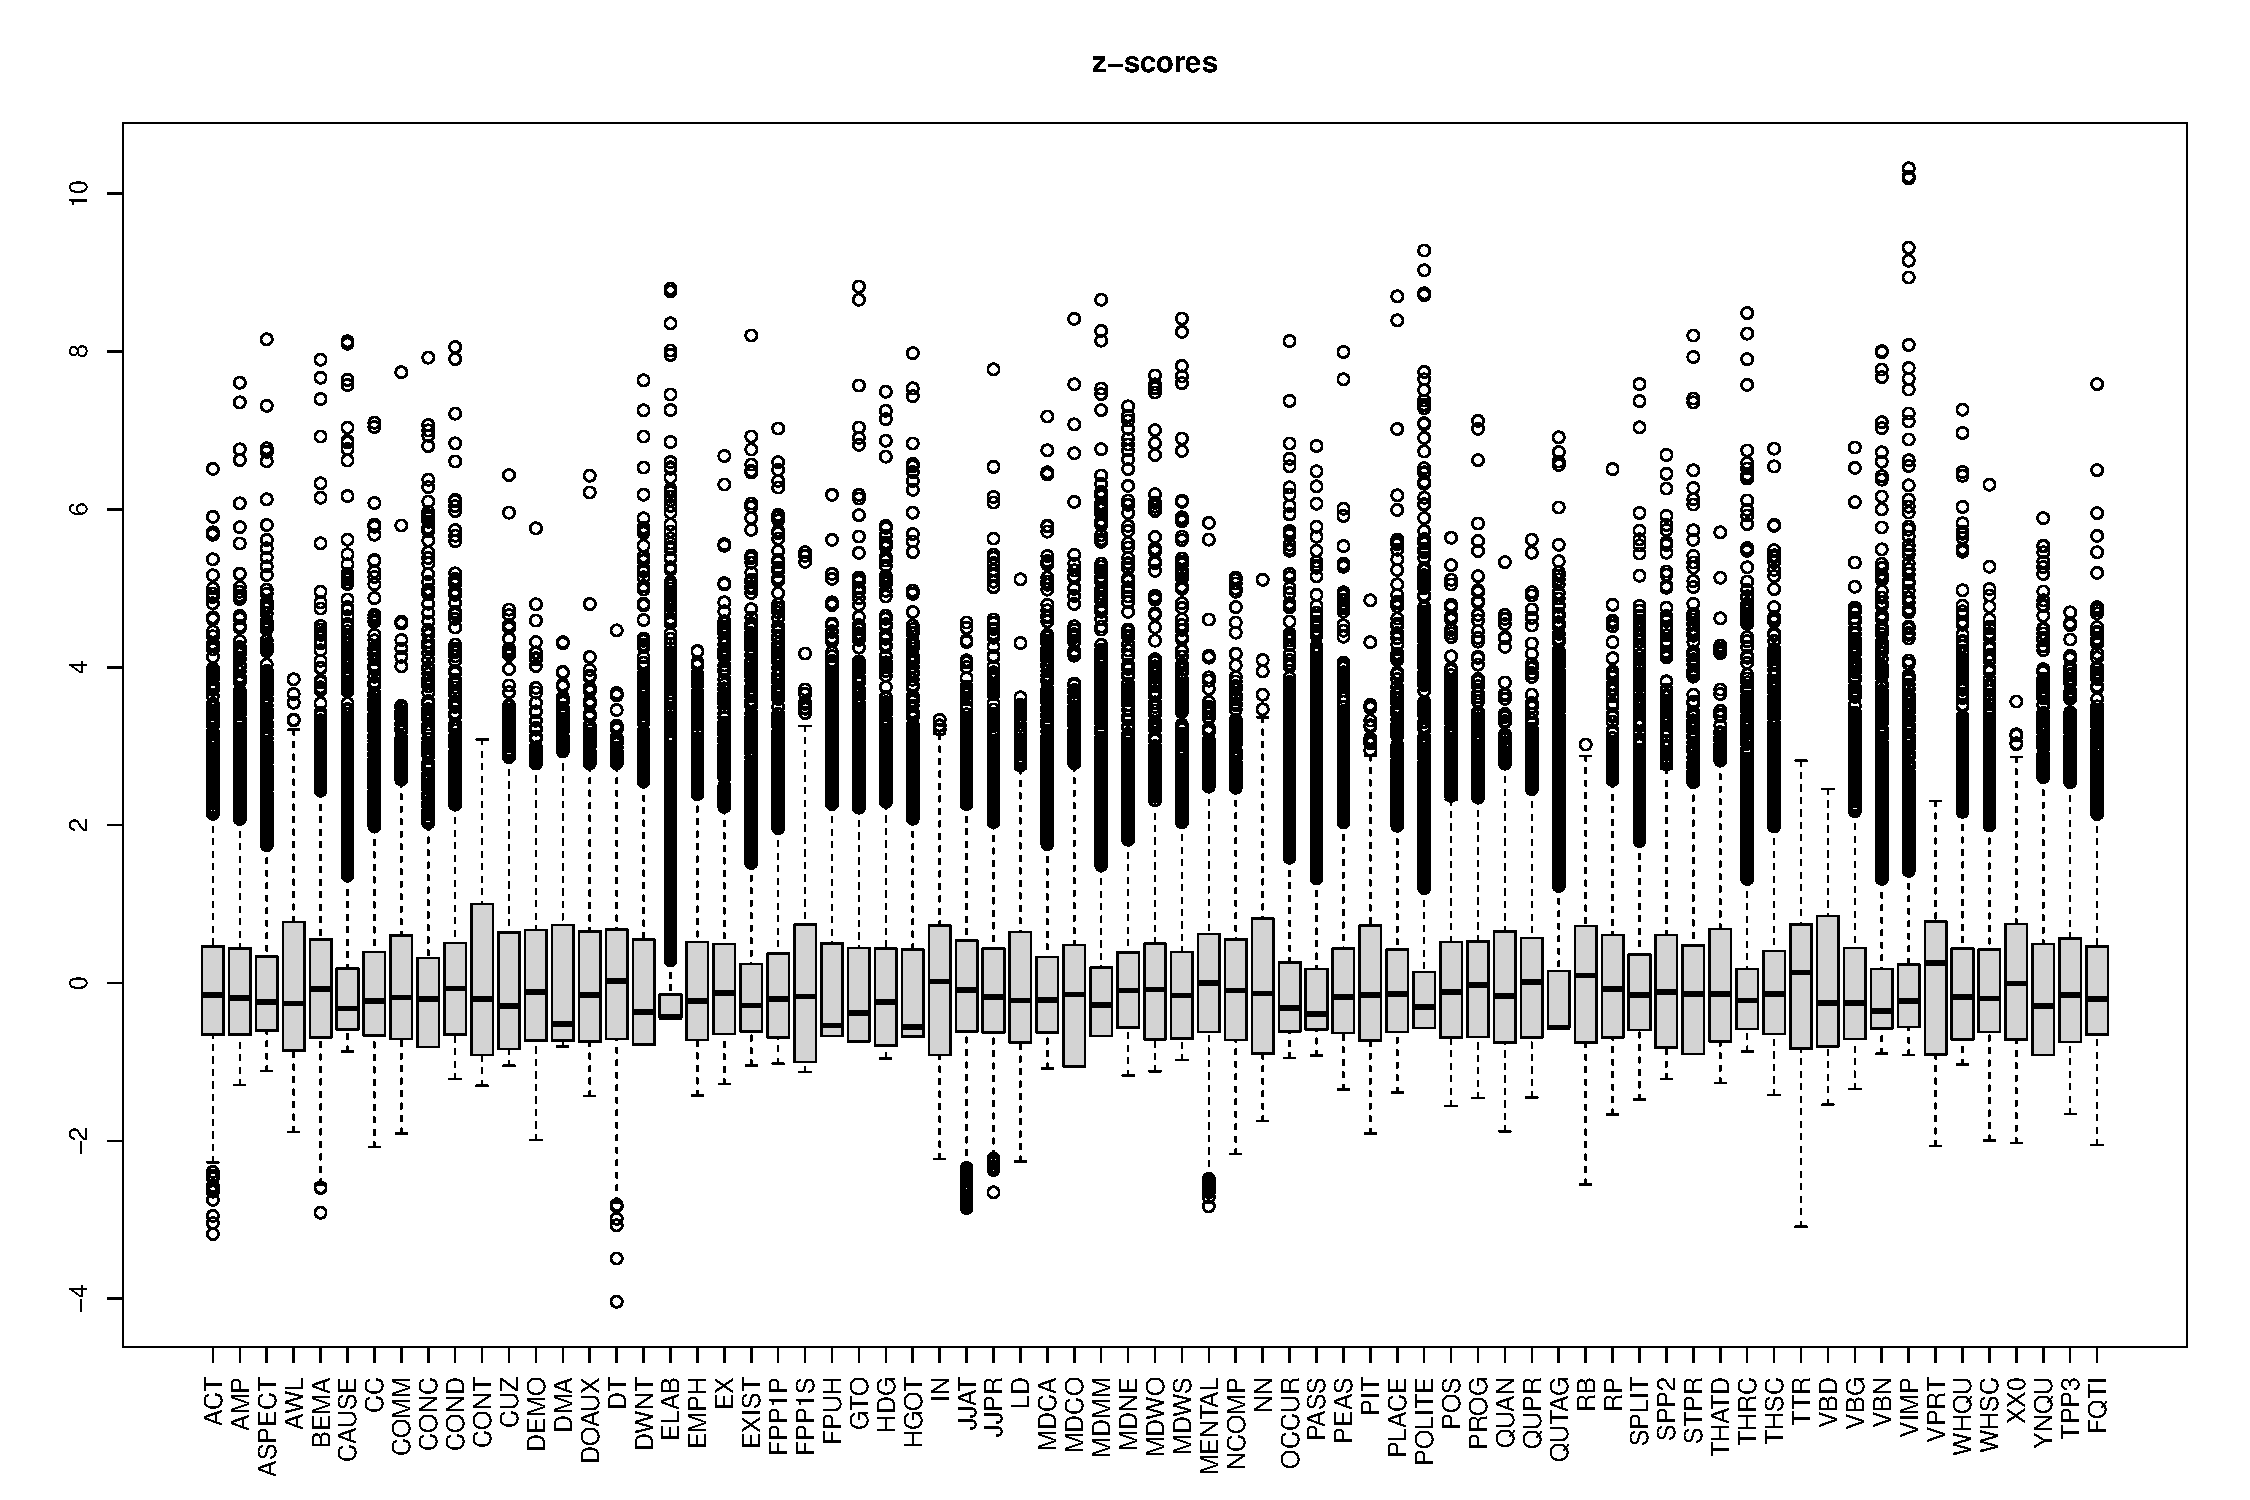
\includegraphics[keepaspectratio]{AppendixG_files/figure-pdf/z-transformed-distributions-1.pdf}}

\subsection{Signed log
transformation}\label{signed-log-transformation-1}

A signed logarithmic transformation was applied to (further) deskew the
feature distributions (see Diwersy, Evert \& Neumann 2014; Neumann \&
Evert 2021).

The signed log transformation function was inspired by the SignedLog
function proposed in
\url{https://cran.r-project.org/web/packages/DataVisualizations/DataVisualizations.pdf}.

\begin{Shaded}
\begin{Highlighting}[]
\NormalTok{signed.log }\OtherTok{\textless{}{-}} \ControlFlowTok{function}\NormalTok{(x) \{}\FunctionTok{sign}\NormalTok{(x)}\SpecialCharTok{*}\FunctionTok{log}\NormalTok{(}\FunctionTok{abs}\NormalTok{(x)}\SpecialCharTok{+}\DecValTok{1}\NormalTok{)\}}

\CommentTok{\# Standardise first, then sign log transform}
\NormalTok{zlogcounts }\OtherTok{\textless{}{-}} \FunctionTok{signed.log}\NormalTok{(zcounts3) }
\end{Highlighting}
\end{Shaded}

The new feature distributions are visualised below.

\begin{Shaded}
\begin{Highlighting}[]
\NormalTok{zlogcounts }\SpecialCharTok{|\textgreater{}}
  \FunctionTok{as.data.frame}\NormalTok{() }\SpecialCharTok{|\textgreater{}} 
  \FunctionTok{gather}\NormalTok{() }\SpecialCharTok{|\textgreater{}} \CommentTok{\# This function from tidyr converts a selection of variables into two variables: a key and a value. The key contains the names of the original variable and the value the data. This means we can then use the facet\_wrap function from ggplot2}
  \FunctionTok{ggplot}\NormalTok{(}\FunctionTok{aes}\NormalTok{(value, }\FunctionTok{after\_stat}\NormalTok{(density))) }\SpecialCharTok{+}
  \FunctionTok{theme\_bw}\NormalTok{() }\SpecialCharTok{+}
  \FunctionTok{facet\_wrap}\NormalTok{(}\SpecialCharTok{\textasciitilde{}}\NormalTok{ key, }\AttributeTok{scales =} \StringTok{"free"}\NormalTok{, }\AttributeTok{ncol =} \DecValTok{4}\NormalTok{) }\SpecialCharTok{+}
  \FunctionTok{scale\_x\_continuous}\NormalTok{(}\AttributeTok{expand=}\FunctionTok{c}\NormalTok{(}\DecValTok{0}\NormalTok{,}\DecValTok{0}\NormalTok{)) }\SpecialCharTok{+}
  \FunctionTok{scale\_y\_continuous}\NormalTok{(}\AttributeTok{limits =} \FunctionTok{c}\NormalTok{(}\DecValTok{0}\NormalTok{,}\ConstantTok{NA}\NormalTok{)) }\SpecialCharTok{+}
  \FunctionTok{geom\_histogram}\NormalTok{(}\AttributeTok{bins =} \DecValTok{30}\NormalTok{, }\AttributeTok{colour=} \StringTok{"black"}\NormalTok{, }\AttributeTok{fill =} \StringTok{"grey"}\NormalTok{) }\SpecialCharTok{+}
  \FunctionTok{geom\_density}\NormalTok{(}\AttributeTok{colour =} \StringTok{"darkred"}\NormalTok{, }\AttributeTok{weight =} \DecValTok{2}\NormalTok{, }\AttributeTok{fill=}\StringTok{"darkred"}\NormalTok{, }\AttributeTok{alpha =}\NormalTok{ .}\DecValTok{4}\NormalTok{)}
\end{Highlighting}
\end{Shaded}

\pandocbounded{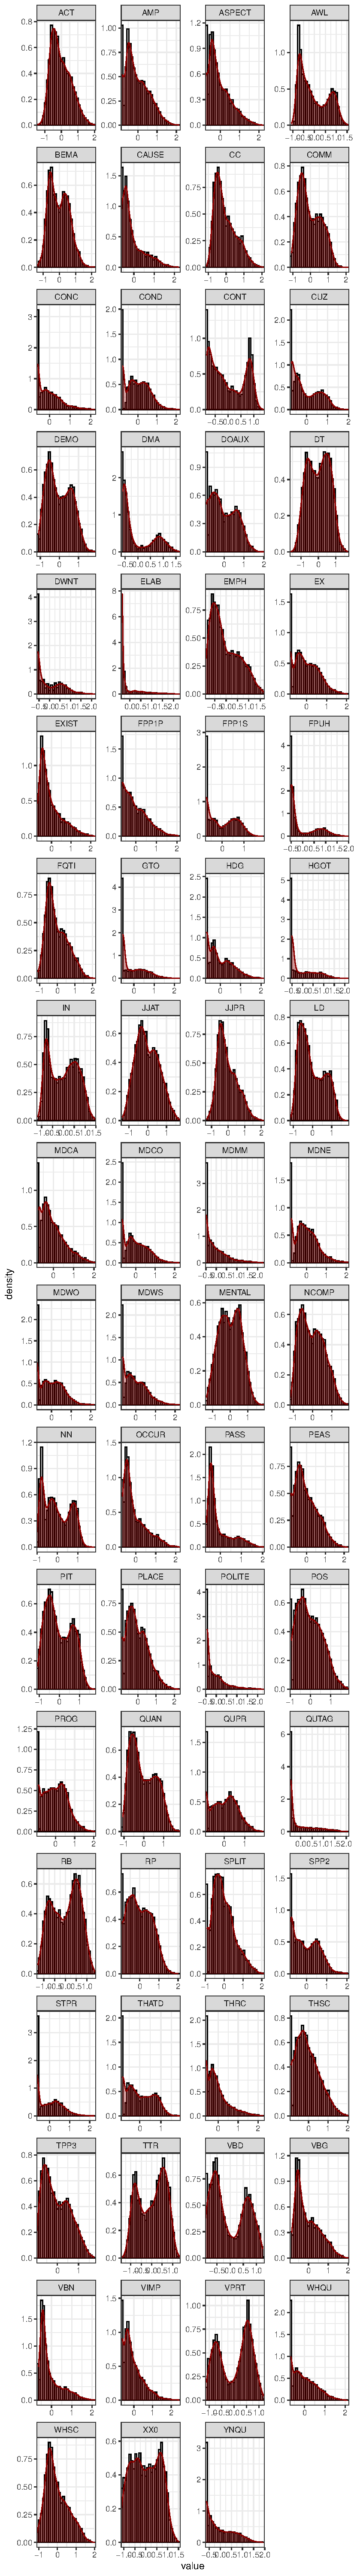
\includegraphics[keepaspectratio]{AppendixG_files/figure-pdf/signed.log.transformation-distributions-1.pdf}}

\begin{Shaded}
\begin{Highlighting}[]
\CommentTok{\#ggsave(here("plots", "DensityPlotsAllVariablesSignedLog.svg"), width = 15, height = 49)}
\end{Highlighting}
\end{Shaded}

\subsection{Merging of data for MDA}\label{merging-of-data-for-mda}

\begin{Shaded}
\begin{Highlighting}[]
\NormalTok{zlogcounts }\OtherTok{\textless{}{-}} \FunctionTok{readRDS}\NormalTok{(}\FunctionTok{here}\NormalTok{(}\StringTok{"data"}\NormalTok{, }\StringTok{"processed"}\NormalTok{, }\StringTok{"zlogcounts\_3Reg.rds"}\NormalTok{)) }
\CommentTok{\#nrow(zlogcounts)}
\CommentTok{\#colnames(zlogcounts)}

\NormalTok{ncounts3 }\OtherTok{\textless{}{-}} \FunctionTok{readRDS}\NormalTok{(}\FunctionTok{here}\NormalTok{(}\StringTok{"data"}\NormalTok{, }\StringTok{"processed"}\NormalTok{, }\StringTok{"ncounts3\_3Reg.rds"}\NormalTok{))}
\CommentTok{\#nrow(ncounts3)}
\CommentTok{\#colnames(ncounts3)}

\NormalTok{data }\OtherTok{\textless{}{-}} \FunctionTok{cbind}\NormalTok{(ncounts3[,}\DecValTok{1}\SpecialCharTok{:}\DecValTok{8}\NormalTok{], }\FunctionTok{as.data.frame}\NormalTok{(zlogcounts))}
\CommentTok{\#saveRDS(data, here("data", "processed", "datazlogcounts\_3Reg.rds")) \# Last saved 16 March 2024}
\end{Highlighting}
\end{Shaded}

The final dataset comprises of 4,980 texts/files, divided as follows:

\begin{longtable}[]{@{}lr@{}}
\toprule\noalign{}
(Sub)corpus & \# texts/files \\
\midrule\noalign{}
\endhead
\bottomrule\noalign{}
\endlastfoot
Textbook Conversation & 565 \\
Textbook Fiction & 285 \\
Info Teens Ref. & 1337 \\
Textbook Informative & 352 \\
Spoken BNC2014 Ref. & 1250 \\
Youth Fiction Ref. & 1191 \\
\end{longtable}

\section{Testing factorability of
data}\label{testing-factorability-of-data}

\subsection{Visualisation of feature
correlations}\label{visualisation-of-feature-correlations}

We begin by visualising the correlations of the transformed feature
frequencies using the \texttt{heatmap} function of the \texttt{stats}
library. Negative correlations are rendered in blue; positive ones are
in red.

\begin{Shaded}
\begin{Highlighting}[]
\CommentTok{\# Simple heatmap in base R (inspired by Stephanie Evert\textquotesingle{}s SIGIL code)}
\NormalTok{cor.colours }\OtherTok{\textless{}{-}} \FunctionTok{c}\NormalTok{(}
  \FunctionTok{hsv}\NormalTok{(}\AttributeTok{h=}\DecValTok{2}\SpecialCharTok{/}\DecValTok{3}\NormalTok{, }\AttributeTok{v=}\DecValTok{1}\NormalTok{, }\AttributeTok{s=}\NormalTok{(}\DecValTok{10}\SpecialCharTok{:}\DecValTok{1}\NormalTok{)}\SpecialCharTok{/}\DecValTok{10}\NormalTok{), }\CommentTok{\# blue = negative correlation }
  \FunctionTok{rgb}\NormalTok{(}\DecValTok{1}\NormalTok{,}\DecValTok{1}\NormalTok{,}\DecValTok{1}\NormalTok{), }\CommentTok{\# white = no correlation }
  \FunctionTok{hsv}\NormalTok{(}\AttributeTok{h=}\DecValTok{0}\NormalTok{, }\AttributeTok{v=}\DecValTok{1}\NormalTok{, }\AttributeTok{s=}\NormalTok{(}\DecValTok{1}\SpecialCharTok{:}\DecValTok{10}\SpecialCharTok{/}\DecValTok{10}\NormalTok{))) }\CommentTok{\# red = positive correlation}

\CommentTok{\#png(here("plots", "heatmapzlogcounts.png"), width = 30, height= 30, units = "cm", res = 300)}
\FunctionTok{heatmap}\NormalTok{(}\FunctionTok{cor}\NormalTok{(zlogcounts), }
        \AttributeTok{symm=}\ConstantTok{TRUE}\NormalTok{, }
        \AttributeTok{zlim=}\FunctionTok{c}\NormalTok{(}\SpecialCharTok{{-}}\DecValTok{1}\NormalTok{,}\DecValTok{1}\NormalTok{), }
        \AttributeTok{col=}\NormalTok{cor.colours, }
        \AttributeTok{margins=}\FunctionTok{c}\NormalTok{(}\DecValTok{7}\NormalTok{,}\DecValTok{7}\NormalTok{))}
\end{Highlighting}
\end{Shaded}

\pandocbounded{
\includegraphics[keepaspectratio]{AppendixG_files/figure-pdf/heatmap-1.pdf}}

\begin{Shaded}
\begin{Highlighting}[]
\CommentTok{\#dev.off()}
\end{Highlighting}
\end{Shaded}

\subsection{Collinearity}\label{collinearity}

As a result of the normalisation unit of finite verb phrases for
verb-based features, the present tense (VPRT) and past tense (VBD)
variables are correlated to a very high degree:

\begin{Shaded}
\begin{Highlighting}[]
\FunctionTok{cor}\NormalTok{(data}\SpecialCharTok{$}\NormalTok{VPRT, data}\SpecialCharTok{$}\NormalTok{VBD) }\SpecialCharTok{|\textgreater{}} \FunctionTok{round}\NormalTok{(}\DecValTok{2}\NormalTok{)}
\end{Highlighting}
\end{Shaded}

\begin{verbatim}
[1] -0.97
\end{verbatim}

We therefore remove the least marked of the pair of collinear variables:
VPRT.

\begin{Shaded}
\begin{Highlighting}[]
\NormalTok{data }\OtherTok{\textless{}{-}}\NormalTok{ data }\SpecialCharTok{|\textgreater{}} 
  \FunctionTok{select}\NormalTok{(}\SpecialCharTok{{-}}\FunctionTok{c}\NormalTok{(VPRT))}
\end{Highlighting}
\end{Shaded}

\subsection{MSA}\label{msa}

\begin{Shaded}
\begin{Highlighting}[]
\NormalTok{kmo }\OtherTok{\textless{}{-}} \FunctionTok{KMO}\NormalTok{(data[,}\DecValTok{9}\SpecialCharTok{:}\FunctionTok{ncol}\NormalTok{(data)]) }\CommentTok{\# The first eight columns contain metadata.}
\end{Highlighting}
\end{Shaded}

The overall MSA value of the dataset is 0.95. The features have the
following individual MSA values (ordered from lowest to largest):

\begin{Shaded}
\begin{Highlighting}[]
\NormalTok{kmo}\SpecialCharTok{$}\NormalTok{MSAi[}\FunctionTok{order}\NormalTok{(kmo}\SpecialCharTok{$}\NormalTok{MSAi)] }\SpecialCharTok{|\textgreater{}}  \FunctionTok{round}\NormalTok{(}\DecValTok{2}\NormalTok{)}
\end{Highlighting}
\end{Shaded}

\begin{verbatim}
   AMP   COMM    POS   TPP3   JJPR  PLACE  SPLIT     DT   JJAT   VIMP   MDCO 
  0.67   0.69   0.70   0.74   0.76   0.82   0.83   0.83   0.84   0.84   0.85 
    RP     EX   THSC     LD  NCOMP   BEMA   MDWS   FQTI  FPP1P   MDCA    ACT 
  0.85   0.85   0.86   0.87   0.88   0.88   0.89   0.89   0.89   0.89   0.89 
MENTAL    VBD  FPP1S   MDMM   PEAS   CONC   MDWO   THRC     NN   COND   PROG 
  0.91   0.91   0.91   0.91   0.91   0.93   0.93   0.94   0.94   0.95   0.95 
    CC   SPP2     RB   DWNT   MDNE   WHSC   CONT   QUPR    XX0  CAUSE   WHQU 
  0.95   0.95   0.95   0.95   0.95   0.96   0.96   0.96   0.96   0.96   0.96 
   VBG    AWL POLITE   PASS    PIT  DOAUX   ELAB ASPECT    DMA   DEMO    HDG 
  0.96   0.96   0.96   0.96   0.97   0.97   0.97   0.97   0.97   0.97   0.97 
    IN   FPUH  OCCUR    CUZ   EMPH   YNQU   QUAN    TTR  QUTAG  THATD    VBN 
  0.97   0.97   0.97   0.97   0.98   0.98   0.98   0.98   0.98   0.98   0.98 
 EXIST   STPR    GTO   HGOT 
  0.98   0.99   0.99   0.99 
\end{verbatim}

We aim to remove features with an individual MSA \textless{} 0.5. All
features have individual MSAs of \textgreater{} 0.5 (but only because
TPP3P was merged into a broader category in an earlier chunk).

\subsection{Scree plot}\label{scree-plot}

Six components were originally retained on the basis of the following
screeplot, though only the first four were found to be interpretable and
were therefore included in the model.

\begin{Shaded}
\begin{Highlighting}[]
\CommentTok{\# png(here("plots", "screeplot{-}TEC{-}Ref\_3Reg.png"), width = 20, height= 12, units = "cm", res = 300)}
\FunctionTok{scree}\NormalTok{(data[,}\DecValTok{9}\SpecialCharTok{:}\FunctionTok{ncol}\NormalTok{(data)], }\AttributeTok{factors =} \ConstantTok{FALSE}\NormalTok{, }\AttributeTok{pc =} \ConstantTok{TRUE}\NormalTok{) }\CommentTok{\# }
\end{Highlighting}
\end{Shaded}

\pandocbounded{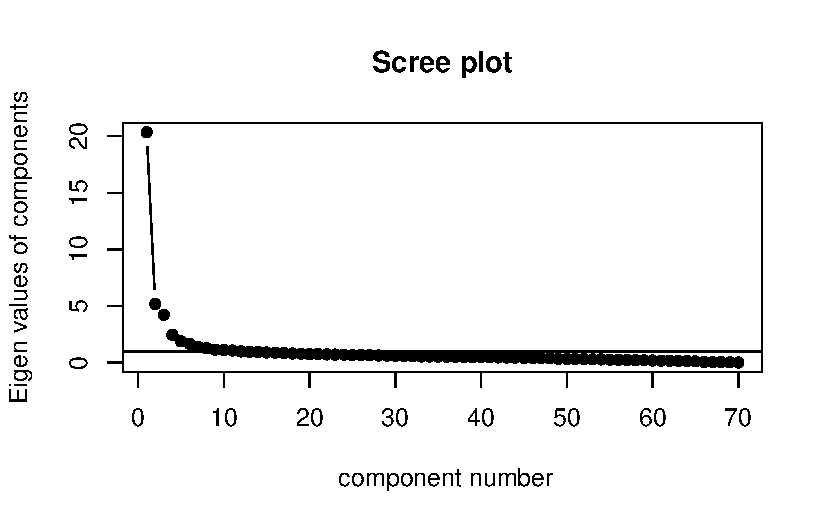
\includegraphics[keepaspectratio]{AppendixG_files/figure-pdf/unnamed-chunk-19-1.pdf}}

\begin{Shaded}
\begin{Highlighting}[]
\CommentTok{\# dev.off()}

\CommentTok{\# Perform PCA}
\NormalTok{pca1 }\OtherTok{\textless{}{-}}\NormalTok{ psych}\SpecialCharTok{::}\FunctionTok{principal}\NormalTok{(data[}\DecValTok{9}\SpecialCharTok{:}\FunctionTok{ncol}\NormalTok{(data)], }
                         \AttributeTok{nfactors =} \DecValTok{6}\NormalTok{)}
\end{Highlighting}
\end{Shaded}

\subsection{Communalities}\label{communalities}

If features with final communalities of \textless{} 0.2 are removed,
TIME would have to be removed. TIME was therefore merged with FREQ in an
earlier chunk so that now all features have final communalities of
\textgreater{} 0.2 (note that this is a very generous threshold!).

\begin{Shaded}
\begin{Highlighting}[]
\NormalTok{pca1}\SpecialCharTok{$}\NormalTok{communality }\SpecialCharTok{|\textgreater{}} \FunctionTok{sort}\NormalTok{() }\SpecialCharTok{|\textgreater{}} \FunctionTok{round}\NormalTok{(}\DecValTok{2}\NormalTok{)}
\end{Highlighting}
\end{Shaded}

\begin{verbatim}
  DWNT   STPR   CONC   FQTI    POS ASPECT   MDNE  FPP1P   PROG   MDCO   MDMM 
  0.22   0.23   0.23   0.23   0.24   0.25   0.27   0.28   0.29   0.32   0.32 
  MDWO  SPLIT   MDWS   PEAS   QUPR    AMP  PLACE    HDG   COMM  CAUSE     EX 
  0.32   0.33   0.34   0.35   0.35   0.35   0.37   0.38   0.38   0.38   0.38 
  THSC  OCCUR   WHSC   THRC   JJAT   COND MENTAL    ACT   VIMP   ELAB  EXIST 
  0.40   0.40   0.42   0.43   0.44   0.44   0.45   0.45   0.46   0.46   0.46 
  JJPR  NCOMP     RP    GTO   DEMO   MDCA POLITE    CUZ     CC   WHQU   TPP3 
  0.46   0.48   0.49   0.50   0.50   0.52   0.52   0.53   0.57   0.58   0.58 
   VBG  THATD    PIT   BEMA  FPP1S     DT   HGOT     RB    VBN  QUTAG   EMPH 
  0.60   0.60   0.61   0.61   0.61   0.61   0.62   0.62   0.64   0.64   0.64 
  PASS    XX0   QUAN   SPP2  DOAUX    TTR   YNQU    VBD     LD   FPUH     IN 
  0.65   0.65   0.67   0.68   0.69   0.71   0.74   0.78   0.81   0.83   0.86 
  CONT    DMA    AWL     NN 
  0.89   0.89   0.91   0.93 
\end{verbatim}

\begin{Shaded}
\begin{Highlighting}[]
\CommentTok{\#saveRDS(data, here("data", "processed", "dataforPCA.rds")) \# Last saved on 6 March 2024}
\end{Highlighting}
\end{Shaded}

The final dataset entered in the analysis described in Chapter 7
therefore comprises 4,980 texts/files, each with logged standardised
normalised frequencies for 70 linguistic features.

\section{Packages used in this
script}\label{packages-used-in-this-script-3}

\subsection{Package names and
versions}\label{package-names-and-versions-3}

\begin{verbatim}
R version 4.4.1 (2024-06-14)
Platform: aarch64-apple-darwin20
Running under: macOS Sonoma 14.5

Matrix products: default
BLAS:   /Library/Frameworks/R.framework/Versions/4.4-arm64/Resources/lib/libRblas.0.dylib 
LAPACK: /Library/Frameworks/R.framework/Versions/4.4-arm64/Resources/lib/libRlapack.dylib;  LAPACK version 3.12.0

locale:
[1] en_US.UTF-8/en_US.UTF-8/en_US.UTF-8/C/en_US.UTF-8/en_US.UTF-8

time zone: Europe/Madrid
tzcode source: internal

attached base packages:
[1] stats     graphics  grDevices datasets  utils     methods   base     

other attached packages:
 [1] DT_0.33             visreg_2.7.0        lubridate_1.9.3    
 [4] forcats_1.0.0       stringr_1.5.1       dplyr_1.1.4        
 [7] purrr_1.0.2         readr_2.1.5         tidyr_1.3.1        
[10] tibble_3.2.1        tidyverse_2.0.0     sjPlot_2.8.16      
[13] scales_1.3.0        psych_2.4.6.26      lme4_1.1-35.5      
[16] Matrix_1.7-0        knitr_1.48          here_1.0.1         
[19] gridExtra_2.3       GGally_2.2.1        ggplot2_3.5.1      
[22] emmeans_1.10.3      cowplot_1.1.3       corrplot_0.92      
[25] car_3.1-2           carData_3.0-5       broom.mixed_0.2.9.5

loaded via a namespace (and not attached):
 [1] tidyselect_1.2.1    sjlabelled_1.2.0    fastmap_1.2.0      
 [4] sjstats_0.19.0      digest_0.6.36       timechange_0.3.0   
 [7] estimability_1.5.1  lifecycle_1.0.4     magrittr_2.0.3     
[10] compiler_4.4.1      rlang_1.1.4         tools_4.4.1        
[13] utf8_1.2.4          yaml_2.3.9          htmlwidgets_1.6.4  
[16] mnormt_2.1.1        plyr_1.8.9          RColorBrewer_1.1-3 
[19] abind_1.4-5         withr_3.0.0         grid_4.4.1         
[22] datawizard_0.12.1   fansi_1.0.6         xtable_1.8-4       
[25] colorspace_2.1-0    future_1.33.2       globals_0.16.3     
[28] MASS_7.3-60.2       insight_0.20.2      cli_3.6.3          
[31] mvtnorm_1.2-5       rmarkdown_2.27      generics_0.1.3     
[34] rstudioapi_0.16.0   performance_0.12.2  tzdb_0.4.0         
[37] minqa_1.2.7         splines_4.4.1       parallel_4.4.1     
[40] BiocManager_1.30.23 vctrs_0.6.5         boot_1.3-30        
[43] jsonlite_1.8.8      hms_1.1.3           listenv_0.9.1      
[46] glue_1.7.0          parallelly_1.37.1   nloptr_2.1.1       
[49] ggstats_0.6.0       codetools_0.2-20    stringi_1.8.4      
[52] gtable_0.3.5        ggeffects_1.7.0     munsell_0.5.1      
[55] furrr_0.3.1         pillar_1.9.0        htmltools_0.5.8.1  
[58] R6_2.5.1            rprojroot_2.0.4     evaluate_0.24.0    
[61] lattice_0.22-6      backports_1.5.0     broom_1.0.6        
[64] renv_1.0.3          Rcpp_1.0.13         coda_0.19-4.1      
[67] nlme_3.1-164        xfun_0.46           sjmisc_2.8.10      
[70] pkgconfig_2.0.3    
\end{verbatim}

\subsection{Package references}\label{package-references-3}

{[}1{]} B. Auguie. \emph{gridExtra: Miscellaneous Functions for ``Grid''
Graphics}. R package version 2.3. 2017.

{[}2{]} D. Bates, M. Mächler, B. Bolker, et al.~``Fitting Linear
Mixed-Effects Models Using lme4''. In: \emph{Journal of Statistical
Software} 67.1 (2015), pp.~1-48. DOI: 10.18637/jss.v067.i01.

{[}3{]} D. Bates, M. Maechler, B. Bolker, et al.~\emph{lme4: Linear
Mixed-Effects Models using Eigen and S4}. R package version 1.1-35.5.
2024. \url{https://github.com/lme4/lme4/}.

{[}4{]} D. Bates, M. Maechler, and M. Jagan. \emph{Matrix: Sparse and
Dense Matrix Classes and Methods}. R package version 1.7-0. 2024.
\url{https://Matrix.R-forge.R-project.org}.

{[}5{]} B. Bolker and D. Robinson. \emph{broom.mixed: Tidying Methods
for Mixed Models}. R package version 0.2.9.5. 2024.
\url{https://github.com/bbolker/broom.mixed}.

{[}6{]} P. Breheny and W. Burchett. \emph{visreg: Visualization of
Regression Models}. R package version 2.7.0. 2020.
\url{http://pbreheny.github.io/visreg}.

{[}7{]} P. Breheny and W. Burchett. ``Visualization of Regression Models
Using visreg''. In: \emph{The R Journal} 9.2 (2017), pp.~56-71.

{[}8{]} J. Fox and S. Weisberg. \emph{An R Companion to Applied
Regression}. Third. Thousand Oaks CA: Sage, 2019.
\url{https://socialsciences.mcmaster.ca/jfox/Books/Companion/}.

{[}9{]} J. Fox, S. Weisberg, and B. Price. \emph{car: Companion to
Applied Regression}. R package version 3.1-2. 2023.
\url{https://r-forge.r-project.org/projects/car/}.

{[}10{]} J. Fox, S. Weisberg, and B. Price. \emph{carData: Companion to
Applied Regression Data Sets}. R package version 3.0-5. 2022.
\url{https://r-forge.r-project.org/projects/car/}.

{[}11{]} G. Grolemund and H. Wickham. ``Dates and Times Made Easy with
lubridate''. In: \emph{Journal of Statistical Software} 40.3 (2011), pp.
1-25. \url{https://www.jstatsoft.org/v40/i03/}.

{[}12{]} R. V. Lenth. \emph{emmeans: Estimated Marginal Means, aka
Least-Squares Means}. R package version 1.10.3. 2024.
\url{https://rvlenth.github.io/emmeans/}.

{[}13{]} D. Lüdecke. \emph{sjPlot: Data Visualization for Statistics in
Social Science}. R package version 2.8.16. 2024.
\url{https://strengejacke.github.io/sjPlot/}.

{[}14{]} K. Müller. \emph{here: A Simpler Way to Find Your Files}. R
package version 1.0.1. 2020. \url{https://here.r-lib.org/}.

{[}15{]} K. Müller and H. Wickham. \emph{tibble: Simple Data Frames}. R
package version 3.2.1. 2023. \url{https://tibble.tidyverse.org/}.

{[}16{]} R Core Team. \emph{R: A Language and Environment for
Statistical Computing}. R Foundation for Statistical Computing. Vienna,
Austria, 2024. \url{https://www.R-project.org/}.

{[}17{]} W. Revelle. \emph{psych: Procedures for Psychological,
Psychometric, and Personality Research}. R package version 2.4.6.26.
2024. \url{https://personality-project.org/r/psych/}.

{[}18{]} B. Schloerke, D. Cook, J. Larmarange, et al.~\emph{GGally:
Extension to ggplot2}. R package version 2.2.1. 2024.
\url{https://ggobi.github.io/ggally/}.

{[}19{]} V. Spinu, G. Grolemund, and H. Wickham. \emph{lubridate: Make
Dealing with Dates a Little Easier}. R package version 1.9.3. 2023.
\url{https://lubridate.tidyverse.org}.

{[}20{]} T. Wei and V. Simko. \emph{corrplot: Visualization of a
Correlation Matrix}. R package version 0.92. 2021.
\url{https://github.com/taiyun/corrplot}.

{[}21{]} T. Wei and V. Simko. \emph{R package `corrplot': Visualization
of a Correlation Matrix}. (Version 0.92). 2021.
\url{https://github.com/taiyun/corrplot}.

{[}22{]} H. Wickham. \emph{forcats: Tools for Working with Categorical
Variables (Factors)}. R package version 1.0.0. 2023.
\url{https://forcats.tidyverse.org/}.

{[}23{]} H. Wickham. \emph{ggplot2: Elegant Graphics for Data Analysis}.
Springer-Verlag New York, 2016. ISBN: 978-3-319-24277-4.
\url{https://ggplot2.tidyverse.org}.

{[}24{]} H. Wickham. \emph{stringr: Simple, Consistent Wrappers for
Common String Operations}. R package version 1.5.1. 2023.
\url{https://stringr.tidyverse.org}.

{[}25{]} H. Wickham. \emph{tidyverse: Easily Install and Load the
Tidyverse}. R package version 2.0.0. 2023.
\url{https://tidyverse.tidyverse.org}.

{[}26{]} H. Wickham, M. Averick, J. Bryan, et al.~``Welcome to the
tidyverse''. In: \emph{Journal of Open Source Software} 4.43 (2019),
p.~1686. DOI: 10.21105/joss.01686.

{[}27{]} H. Wickham, W. Chang, L. Henry, et al.~\emph{ggplot2: Create
Elegant Data Visualisations Using the Grammar of Graphics}. R package
version 3.5.1. 2024. \url{https://ggplot2.tidyverse.org}.

{[}28{]} H. Wickham, R. François, L. Henry, et al.~\emph{dplyr: A
Grammar of Data Manipulation}. R package version 1.1.4. 2023.
\url{https://dplyr.tidyverse.org}.

{[}29{]} H. Wickham and L. Henry. \emph{purrr: Functional Programming
Tools}. R package version 1.0.2. 2023.
\url{https://purrr.tidyverse.org/}.

{[}30{]} H. Wickham, J. Hester, and J. Bryan. \emph{readr: Read
Rectangular Text Data}. R package version 2.1.5. 2024.
\url{https://readr.tidyverse.org}.

{[}31{]} H. Wickham, T. L. Pedersen, and D. Seidel. \emph{scales: Scale
Functions for Visualization}. R package version 1.3.0. 2023.
\url{https://scales.r-lib.org}.

{[}32{]} H. Wickham, D. Vaughan, and M. Girlich. \emph{tidyr: Tidy Messy
Data}. R package version 1.3.1. 2024. \url{https://tidyr.tidyverse.org}.

{[}33{]} C. O. Wilke. \emph{cowplot: Streamlined Plot Theme and Plot
Annotations for ggplot2}. R package version 1.1.3. 2024.
\url{https://wilkelab.org/cowplot/}.

{[}34{]} Y. Xie. \emph{Dynamic Documents with R and knitr}. 2nd. ISBN
978-1498716963. Boca Raton, Florida: Chapman and Hall/CRC, 2015.
\url{https://yihui.org/knitr/}.

{[}35{]} Y. Xie. ``knitr: A Comprehensive Tool for Reproducible Research
in R''. In: \emph{Implementing Reproducible Computational Research}. Ed.
by V. Stodden, F. Leisch and R. D. Peng. ISBN 978-1466561595. Chapman
and Hall/CRC, 2014.

{[}36{]} Y. Xie. \emph{knitr: A General-Purpose Package for Dynamic
Report Generation in R}. R package version 1.48. 2024.
\url{https://yihui.org/knitr/}.

{[}37{]} Y. Xie, J. Cheng, and X. Tan. \emph{DT: A Wrapper of the
JavaScript Library DataTables}. R package version 0.33. 2024.
\url{https://github.com/rstudio/DT}.

\chapter{Data Analysis for the Model of Textbook English
vs.~`real-world'
English}\label{data-analysis-for-the-model-of-textbook-english-vs.-real-world-english}

This script documents the analysis of data from the TEC and reference
corpus data (as pre-processed in Appendix F) to arrive at the
multi-dimensional model of Textbook Englisch vs.~`real-world' English
described in Chapter 7. It generates all of the statistics and plots
included in the book, as well as many others that were used in the
analysis, but were not included in the book for reasons of space.

\section{Packages required}\label{packages-required-3}

The following packages must be installed and loaded to process the data.

\begin{Shaded}
\begin{Highlighting}[]
\CommentTok{\#renv::restore() \# Restore the project\textquotesingle{}s dependencies from the lockfile to ensure that same package versions are used as in the original thesis.}

\FunctionTok{library}\NormalTok{(caret) }\CommentTok{\# For its confusion matrix function}
\FunctionTok{library}\NormalTok{(cowplot) }\CommentTok{\# For its plot themes}
\FunctionTok{library}\NormalTok{(DescTools) }\CommentTok{\# For 95\% CI}
\FunctionTok{library}\NormalTok{(emmeans) }\CommentTok{\# For the emmeans function}
\FunctionTok{library}\NormalTok{(factoextra) }\CommentTok{\# For circular graphs of variables}
\FunctionTok{library}\NormalTok{(gtsummary) }\CommentTok{\# For nice table of summary statistics (optional)}
\FunctionTok{library}\NormalTok{(gridExtra) }\CommentTok{\# For Fig. 35}
\FunctionTok{library}\NormalTok{(here) }\CommentTok{\# For dynamic file paths}
\FunctionTok{library}\NormalTok{(ggthemes) }\CommentTok{\# For theme of factoextra plots}
\FunctionTok{library}\NormalTok{(knitr) }\CommentTok{\# Loaded to display the tables using the kable() function}
\FunctionTok{library}\NormalTok{(lme4) }\CommentTok{\# For linear regression modelling}
\FunctionTok{library}\NormalTok{(patchwork) }\CommentTok{\# To create figures with more than one plot}
\CommentTok{\#library(pca3d) \# For 3{-}D plots (not rendered in exports)}
\FunctionTok{library}\NormalTok{(PCAtools) }\CommentTok{\# For nice biplots of PCA results}
\FunctionTok{library}\NormalTok{(psych) }\CommentTok{\# For various useful stats function}
\FunctionTok{library}\NormalTok{(sjPlot) }\CommentTok{\# For model plots and tables}
\FunctionTok{library}\NormalTok{(tidyverse) }\CommentTok{\# For data wrangling}
\FunctionTok{library}\NormalTok{(visreg) }\CommentTok{\# For plots of interaction effects}

\FunctionTok{source}\NormalTok{(}\FunctionTok{here}\NormalTok{(}\StringTok{"R\_rainclouds.R"}\NormalTok{)) }\CommentTok{\# For geom\_flat\_violin rainplots}
\end{Highlighting}
\end{Shaded}

\section{Conducting the PCA}\label{conducting-the-pca}

We first import the full dataset (see Appendix F for data preparation
steps).

The following chunks can be used to perform the MDA on various subsets
of the data (see also Section 10.1.1 in the book).

\begin{enumerate}
\def\labelenumi{\roman{enumi}.}
\tightlist
\item
  Subset of the data that excludes the lower-level textbooks:
\end{enumerate}

\begin{Shaded}
\begin{Highlighting}[]
\NormalTok{data }\OtherTok{\textless{}{-}} \FunctionTok{readRDS}\NormalTok{(}\FunctionTok{here}\NormalTok{(}\StringTok{"processed\_data"}\NormalTok{, }\StringTok{"dataforPCA.rds"}\NormalTok{)) }\SpecialCharTok{|\textgreater{}}
  \FunctionTok{filter}\NormalTok{(Level }\SpecialCharTok{!=}\StringTok{"A"} \SpecialCharTok{\&}\NormalTok{ Level }\SpecialCharTok{!=} \StringTok{"B"}\NormalTok{) }\SpecialCharTok{|\textgreater{}}
  \FunctionTok{droplevels}\NormalTok{()}
\FunctionTok{summary}\NormalTok{(data}\SpecialCharTok{$}\NormalTok{Level)}
\end{Highlighting}
\end{Shaded}

\begin{enumerate}
\def\labelenumi{\roman{enumi}.}
\tightlist
\item
  Subset of the data that includes only one \texttt{Country}` subcorpus
  of the TEC (note that a detailed analysis of the German subcorpus can
  be found in (Le Foll)):
\end{enumerate}

\begin{Shaded}
\begin{Highlighting}[]
\NormalTok{data }\OtherTok{\textless{}{-}} \FunctionTok{readRDS}\NormalTok{(}\FunctionTok{here}\NormalTok{(}\StringTok{"processed\_data"}\NormalTok{, }\StringTok{"dataforPCA.rds"}\NormalTok{)) }\SpecialCharTok{|\textgreater{}}
  \CommentTok{\#filter(Country != "France" \& Country != "Germany") |\textgreater{} \# Spain only}
  \CommentTok{\#filter(Country != "France" \& Country != "Spain") |\textgreater{} \# Germany only}
  \FunctionTok{filter}\NormalTok{(Country }\SpecialCharTok{!=} \StringTok{"Spain"} \SpecialCharTok{\&}\NormalTok{ Country }\SpecialCharTok{!=} \StringTok{"Germany"}\NormalTok{) }\SpecialCharTok{|\textgreater{}} \CommentTok{\# France only}
  \FunctionTok{droplevels}\NormalTok{()}
\FunctionTok{summary}\NormalTok{(data}\SpecialCharTok{$}\NormalTok{Country)}
\end{Highlighting}
\end{Shaded}

\begin{enumerate}
\def\labelenumi{\roman{enumi}.}
\tightlist
\item
  Random subsets of the data to test the stability of the model proposed
  in Chapter 7. Re-running this line will generate a new subset of 2/3
  of the texts randomly sampled. \texttt{set.seed(13)} was used for the
  analyses reported on in Section 10.1.1.
\end{enumerate}

\begin{Shaded}
\begin{Highlighting}[]
\FunctionTok{set.seed}\NormalTok{(}\DecValTok{13}\NormalTok{) }
\NormalTok{data }\OtherTok{\textless{}{-}} \FunctionTok{readRDS}\NormalTok{(}\FunctionTok{here}\NormalTok{(}\StringTok{"processed\_data"}\NormalTok{, }\StringTok{"dataforPCA.rds"}\NormalTok{)) }\SpecialCharTok{|\textgreater{}}
  \FunctionTok{slice\_sample}\NormalTok{(}\AttributeTok{n =} \DecValTok{4980}\SpecialCharTok{*}\FloatTok{0.6}\NormalTok{, }\AttributeTok{replace =} \ConstantTok{FALSE}\NormalTok{)}
\FunctionTok{nrow}\NormalTok{(data)}
\NormalTok{data}\SpecialCharTok{$}\NormalTok{Filename[}\DecValTok{1}\SpecialCharTok{:}\DecValTok{4}\NormalTok{]}
\CommentTok{\#Using the set.seed(13), these should be:}
\CommentTok{\#[1] HT\_4\_Spoken\_0009.txt                       }
\CommentTok{\#[2] Solutions\_Intermediate\_Plus\_Spoken\_0020.txt}
\CommentTok{\#[3] 141\_PRATCHETT1992DW13GODS\_4.txt            }
\CommentTok{\#[4] Achievers\_B2\_Informative\_0004.txt}
\end{Highlighting}
\end{Shaded}

\section{Plotting PCA results}\label{plotting-pca-results-1}

\subsection{3D plots}\label{d-plots-1}

The following chunk can be used to create projections of TEC texts on
three dimensions of the model. These plots cannot be rendered in two
dimensions and are therefore not generated in the present document. For
more information on the \texttt{pca3d} library, see:
\url{https://cran.r-project.org/web/packages/pca3d/vignettes/pca3d.pdf}.

\begin{Shaded}
\begin{Highlighting}[]
\CommentTok{\# Data preparation for 3D plots}
\FunctionTok{colnames}\NormalTok{(data) }\CommentTok{\# Checking that the features start at the 9th column}
\NormalTok{pca }\OtherTok{\textless{}{-}} \FunctionTok{prcomp}\NormalTok{(data[,}\DecValTok{9}\SpecialCharTok{:}\FunctionTok{ncol}\NormalTok{(data)], }\AttributeTok{scale.=}\ConstantTok{FALSE}\NormalTok{) }\CommentTok{\# All quantitative variables that contribute to the model}
\NormalTok{register }\OtherTok{\textless{}{-}} \FunctionTok{factor}\NormalTok{(data[,}\StringTok{"Register"}\NormalTok{]) }
\NormalTok{corpus }\OtherTok{\textless{}{-}} \FunctionTok{factor}\NormalTok{(data[,}\StringTok{"Corpus"}\NormalTok{])}
\NormalTok{subcorpus }\OtherTok{\textless{}{-}} \FunctionTok{factor}\NormalTok{(data[,}\StringTok{"Subcorpus"}\NormalTok{])}

\FunctionTok{library}\NormalTok{(pca3d)}

\FunctionTok{pca3d}\NormalTok{(pca, }\AttributeTok{group =}\NormalTok{ subcorpus,}
       \AttributeTok{components =} \DecValTok{1}\SpecialCharTok{:}\DecValTok{3}\NormalTok{,}
       \AttributeTok{components =} \DecValTok{4}\SpecialCharTok{:}\DecValTok{6}\NormalTok{,}
       \AttributeTok{show.plane=}\ConstantTok{FALSE}\NormalTok{,}
       \AttributeTok{col =}\NormalTok{ col6,}
       \AttributeTok{shape =}\NormalTok{ shapes6,}
       \AttributeTok{radius =} \FloatTok{0.7}\NormalTok{,}
       \AttributeTok{legend =} \StringTok{"right"}\NormalTok{)}

\FunctionTok{snapshotPCA3d}\NormalTok{(}\FunctionTok{here}\NormalTok{(}\StringTok{"plots"}\NormalTok{, }\StringTok{"PCA\_TxB\_3Ref\_3Dsnapshot.png"}\NormalTok{))}

\CommentTok{\# Alternative visualisation, looking at all three Textbook English registers in one colour}

\FunctionTok{pca3d}\NormalTok{(pca, }\AttributeTok{group =}\NormalTok{ corpus, }
      \AttributeTok{show.plane=}\ConstantTok{FALSE}\NormalTok{,}
      \AttributeTok{components =} \DecValTok{1}\SpecialCharTok{:}\DecValTok{3}\NormalTok{,}
      \AttributeTok{col =}\NormalTok{ col4,}
      \AttributeTok{shape =}\NormalTok{ shapes4,}
      \AttributeTok{radius =} \FloatTok{0.7}\NormalTok{,}
      \AttributeTok{legend =} \StringTok{"right"}\NormalTok{)}
\end{Highlighting}
\end{Shaded}

\section{Two-dimensional plots
(biplots)}\label{two-dimensional-plots-biplots-1}

These plots were generated using the \texttt{PCAtools} package, which
requires the data to be formatted in a rather unconventional way so it
needs to wrangled first.

\subsection{Data wrangling for
PCAtools}\label{data-wrangling-for-pcatools-1}

\begin{Shaded}
\begin{Highlighting}[]
\CommentTok{\# Data wrangling}
\NormalTok{data2 }\OtherTok{\textless{}{-}}\NormalTok{ data }\SpecialCharTok{|\textgreater{}} 
  \FunctionTok{mutate}\NormalTok{(}\AttributeTok{Source =} \FunctionTok{recode\_factor}\NormalTok{(Corpus, }\AttributeTok{Textbook.English =} \StringTok{"Textbook English (TEC)"}\NormalTok{, }\AttributeTok{Informative.Teens =} \StringTok{"Reference corpora"}\NormalTok{, }\AttributeTok{Spoken.BNC2014 =} \StringTok{"Reference corpora"}\NormalTok{, }\AttributeTok{Youth.Fiction =} \StringTok{"Reference corpora"}\NormalTok{)) }\SpecialCharTok{|\textgreater{}} 
  \FunctionTok{mutate}\NormalTok{(}\AttributeTok{Corpus =} \FunctionTok{fct\_relevel}\NormalTok{(Subcorpus, }\StringTok{"Info Teens Ref."}\NormalTok{, }\AttributeTok{after =} \DecValTok{9}\NormalTok{)) }\SpecialCharTok{|\textgreater{}}
  \FunctionTok{relocate}\NormalTok{(Source, }\AttributeTok{.after =} \StringTok{"Corpus"}\NormalTok{) }\SpecialCharTok{|\textgreater{}} 
  \FunctionTok{droplevels}\NormalTok{()}

\CommentTok{\# colnames(data2)}
\NormalTok{data2meta }\OtherTok{\textless{}{-}}\NormalTok{ data2[,}\DecValTok{1}\SpecialCharTok{:}\DecValTok{9}\NormalTok{]}
\FunctionTok{rownames}\NormalTok{(data2meta) }\OtherTok{\textless{}{-}}\NormalTok{ data2meta}\SpecialCharTok{$}\NormalTok{Filename}
\NormalTok{data2meta }\OtherTok{\textless{}{-}}\NormalTok{ data2meta }\SpecialCharTok{|\textgreater{}} \FunctionTok{select}\NormalTok{(}\SpecialCharTok{{-}}\NormalTok{Filename)}
\CommentTok{\# head(data2meta)}
\FunctionTok{rownames}\NormalTok{(data2) }\OtherTok{\textless{}{-}}\NormalTok{ data2}\SpecialCharTok{$}\NormalTok{Filename}
\NormalTok{data2num }\OtherTok{\textless{}{-}} \FunctionTok{as.data.frame}\NormalTok{(base}\SpecialCharTok{::}\FunctionTok{t}\NormalTok{(data2[,}\DecValTok{10}\SpecialCharTok{:}\FunctionTok{ncol}\NormalTok{(data2)]))}
\CommentTok{\# data2num[1:5,1:5] \# Check data frame format is correct by comparing to output of head(data2meta) above}

\NormalTok{p }\OtherTok{\textless{}{-}}\NormalTok{ PCAtools}\SpecialCharTok{::}\FunctionTok{pca}\NormalTok{(data2num, }
         \AttributeTok{metadata =}\NormalTok{ data2meta,}
         \AttributeTok{scale =} \ConstantTok{FALSE}\NormalTok{)}
\end{Highlighting}
\end{Shaded}

The cumulative proportion of variance in the dataset explained the first
four components explain 47.15\%.

\subsection{Pairs plot}\label{pairs-plot-1}

This chunk produces a scatterplot matrix of combinations of the four
dimensions of the model of Textbook English vs.~`real-world' English.
Note that the number before the comma on each axis label shows which
principal component is plotted on that axis; this is followed by the
percentage of the total variance explained by that particular component.
The colours correspond to the text registers.

\begin{Shaded}
\begin{Highlighting}[]
\CommentTok{\# For five TEC registers}
\CommentTok{\# colkey = c(\textasciigrave{}Spoken BNC2014 Ref.\textasciigrave{}="\#BD241E", \textasciigrave{}Info Teens Ref.\textasciigrave{}="\#15274D", \textasciigrave{}Youth Fiction Ref.\textasciigrave{}="\#267226", \textasciigrave{}Textbook Fiction\textasciigrave{}="\#A18A33", \textasciigrave{}Textbook Conversation\textasciigrave{}="\#F9B921", \textasciigrave{}Textbook Informative\textasciigrave{} = "\#722672", \textasciigrave{}Textbook Instructional\textasciigrave{} = "grey", \textasciigrave{}Textbook Personal\textasciigrave{} = "black")}

\CommentTok{\# For three TEC registers}
\CommentTok{\# summary(data2$Corpus)}
\NormalTok{colkey }\OtherTok{=} \FunctionTok{c}\NormalTok{(}\StringTok{\textasciigrave{}}\AttributeTok{Spoken BNC2014 Ref.}\StringTok{\textasciigrave{}}\OtherTok{=}\StringTok{"\#BD241E"}\NormalTok{, }\StringTok{\textasciigrave{}}\AttributeTok{Info Teens Ref.}\StringTok{\textasciigrave{}}\OtherTok{=}\StringTok{"\#15274D"}\NormalTok{, }\StringTok{\textasciigrave{}}\AttributeTok{Youth Fiction Ref.}\StringTok{\textasciigrave{}}\OtherTok{=}\StringTok{"\#267226"}\NormalTok{, }\StringTok{\textasciigrave{}}\AttributeTok{Textbook Fiction}\StringTok{\textasciigrave{}}\OtherTok{=}\StringTok{"\#A18A33"}\NormalTok{, }\StringTok{\textasciigrave{}}\AttributeTok{Textbook Conversation}\StringTok{\textasciigrave{}}\OtherTok{=}\StringTok{"\#F9B921"}\NormalTok{, }\StringTok{\textasciigrave{}}\AttributeTok{Textbook Informative}\StringTok{\textasciigrave{}} \OtherTok{=} \StringTok{"\#722672"}\NormalTok{)}

\CommentTok{\#summary(data2$Source)}
\CommentTok{\#shapekey = c(\textasciigrave{}Textbook English (TEC)\textasciigrave{}=6, \textasciigrave{}Reference corpora\textasciigrave{}=1)}

\CommentTok{\# summary(data2$Level)}
\NormalTok{shapekey }\OtherTok{=} \FunctionTok{c}\NormalTok{(}\AttributeTok{A=}\DecValTok{1}\NormalTok{, }\AttributeTok{B=}\DecValTok{2}\NormalTok{, }\AttributeTok{C=}\DecValTok{6}\NormalTok{, }\AttributeTok{D=}\DecValTok{0}\NormalTok{, }\AttributeTok{E=}\DecValTok{5}\NormalTok{, }\StringTok{\textasciigrave{}}\AttributeTok{Ref.}\StringTok{\textasciigrave{}}\OtherTok{=}\DecValTok{4}\NormalTok{)}

\DocumentationTok{\#\# Warning: this can be very slow! Open in extra zoomed out window!}

\CommentTok{\#png(here("plots", "PCA\_3Ref\_pairsplot.png"), width = 12, height= 19, units = "cm", res = 300)}
\NormalTok{PCAtools}\SpecialCharTok{::}\FunctionTok{pairsplot}\NormalTok{(p,}
                 \AttributeTok{triangle =} \ConstantTok{FALSE}\NormalTok{,}
                 \AttributeTok{components =} \DecValTok{1}\SpecialCharTok{:}\DecValTok{4}\NormalTok{,}
                 \AttributeTok{ncol =} \DecValTok{2}\NormalTok{,}
                 \AttributeTok{nrow =} \DecValTok{3}\NormalTok{,}
                 \AttributeTok{pointSize =} \FloatTok{0.6}\NormalTok{,}
                 \AttributeTok{shape =} \StringTok{"Level"}\NormalTok{,}
                 \AttributeTok{shapekey =}\NormalTok{ shapekey,}
                 \AttributeTok{lab =} \ConstantTok{NULL}\NormalTok{, }\CommentTok{\# Otherwise will try to label each data point!}
                 \AttributeTok{colby =} \StringTok{"Corpus"}\NormalTok{,}
                 \AttributeTok{legendPosition =} \StringTok{"none"}\NormalTok{,}
                 \AttributeTok{margingaps =} \FunctionTok{unit}\NormalTok{(}\FunctionTok{c}\NormalTok{(}\FloatTok{0.2}\NormalTok{, }\FloatTok{0.2}\NormalTok{, }\FloatTok{0.8}\NormalTok{, }\FloatTok{0.2}\NormalTok{), }\StringTok{"cm"}\NormalTok{),}
                 \AttributeTok{colkey =}\NormalTok{ colkey)}
\end{Highlighting}
\end{Shaded}

\pandocbounded{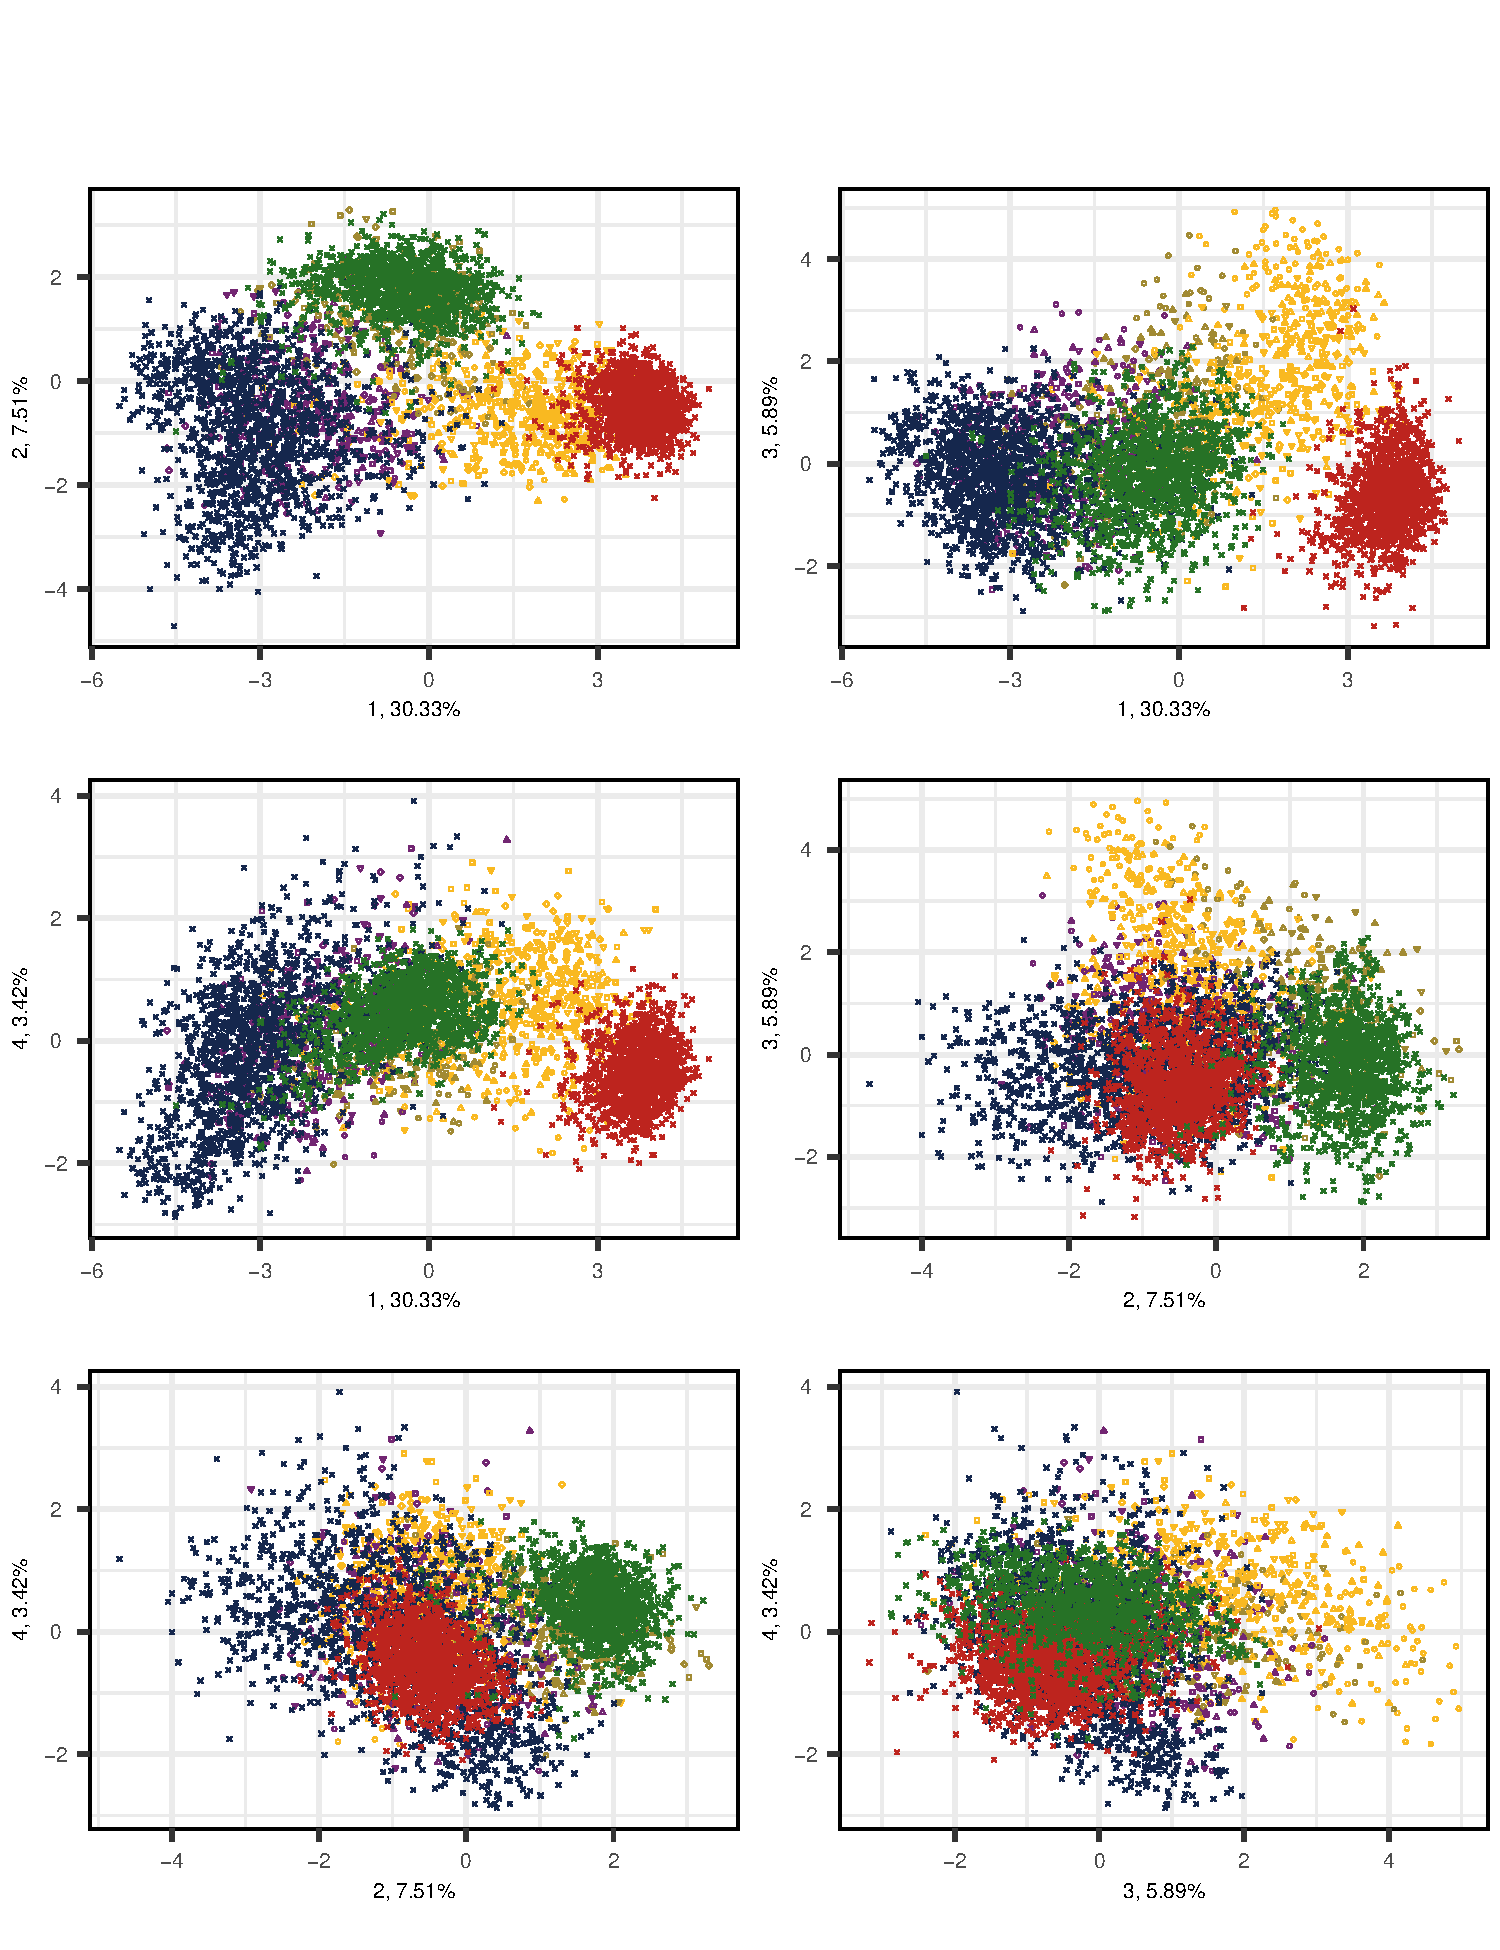
\includegraphics[keepaspectratio]{AppendixH_files/figure-pdf/PCAtools-pairsplots-TxB-1.pdf}}

\begin{Shaded}
\begin{Highlighting}[]
\CommentTok{\#dev.off()}
\CommentTok{\#ggsave(here("plots", "PCA\_TxB\_pairsplot.svg"), width = 6, height = 10)}
\CommentTok{\# Note that the legend has to be added manually (it was taken from the biplot code below).}
\end{Highlighting}
\end{Shaded}

\subsection{Bi-plots}\label{bi-plots-1}

Biplots are used to more closely examine the position of texts on just
two dimensions.

\begin{Shaded}
\begin{Highlighting}[]
\CommentTok{\# These settings (with legendPosition = "top") were used to generate the legend for the scatterplot matrix above:}
\CommentTok{\#png(here("plots", "PCA\_3Ref\_Biplot\_PC1\_PC2test.png"), width = 40, height= 25, units = "cm", res = 300) }

\NormalTok{PCAtools}\SpecialCharTok{::}\FunctionTok{biplot}\NormalTok{(p,}
                 \AttributeTok{x =} \StringTok{"PC1"}\NormalTok{,}
                 \AttributeTok{y =} \StringTok{"PC2"}\NormalTok{,}
                 \AttributeTok{lab =} \ConstantTok{NULL}\NormalTok{, }\CommentTok{\# Otherwise will try to label each data point!}
                 \AttributeTok{colby =} \StringTok{"Corpus"}\NormalTok{,}
                 \AttributeTok{pointSize =} \FloatTok{1.3}\NormalTok{,}
                 \AttributeTok{colkey =}\NormalTok{ colkey,}
                 \AttributeTok{shape =} \StringTok{"Level"}\NormalTok{,}
                 \AttributeTok{shapekey =}\NormalTok{ shapekey,}
                 \AttributeTok{xlim =} \FunctionTok{c}\NormalTok{(}\FunctionTok{min}\NormalTok{(p}\SpecialCharTok{$}\NormalTok{rotated[, }\StringTok{"PC1"}\NormalTok{]), }\FunctionTok{max}\NormalTok{(p}\SpecialCharTok{$}\NormalTok{rotated[, }\StringTok{"PC1"}\NormalTok{])),}
                 \AttributeTok{ylim =} \FunctionTok{c}\NormalTok{(}\FunctionTok{min}\NormalTok{(p}\SpecialCharTok{$}\NormalTok{rotated[, }\StringTok{"PC2"}\NormalTok{]), }\FunctionTok{max}\NormalTok{(p}\SpecialCharTok{$}\NormalTok{rotated[, }\StringTok{"PC2"}\NormalTok{])),}
                 \AttributeTok{showLoadings =} \ConstantTok{FALSE}\NormalTok{,}
                 \AttributeTok{ellipse =} \ConstantTok{TRUE}\NormalTok{,}
                 \AttributeTok{axisLabSize =} \DecValTok{18}\NormalTok{,}
                 \AttributeTok{legendPosition =} \StringTok{\textquotesingle{}right\textquotesingle{}}\NormalTok{,}
                 \AttributeTok{legendTitleSize =} \DecValTok{18}\NormalTok{,}
                 \AttributeTok{legendLabSize =} \DecValTok{14}\NormalTok{, }
                 \AttributeTok{legendIconSize =} \DecValTok{5}\NormalTok{) }\SpecialCharTok{+}
  \FunctionTok{theme}\NormalTok{(}\AttributeTok{plot.margin =} \FunctionTok{unit}\NormalTok{(}\FunctionTok{c}\NormalTok{(}\DecValTok{0}\NormalTok{,}\DecValTok{0}\NormalTok{,}\DecValTok{0}\NormalTok{,}\FloatTok{0.2}\NormalTok{), }\StringTok{"cm"}\NormalTok{))}
\end{Highlighting}
\end{Shaded}

\pandocbounded{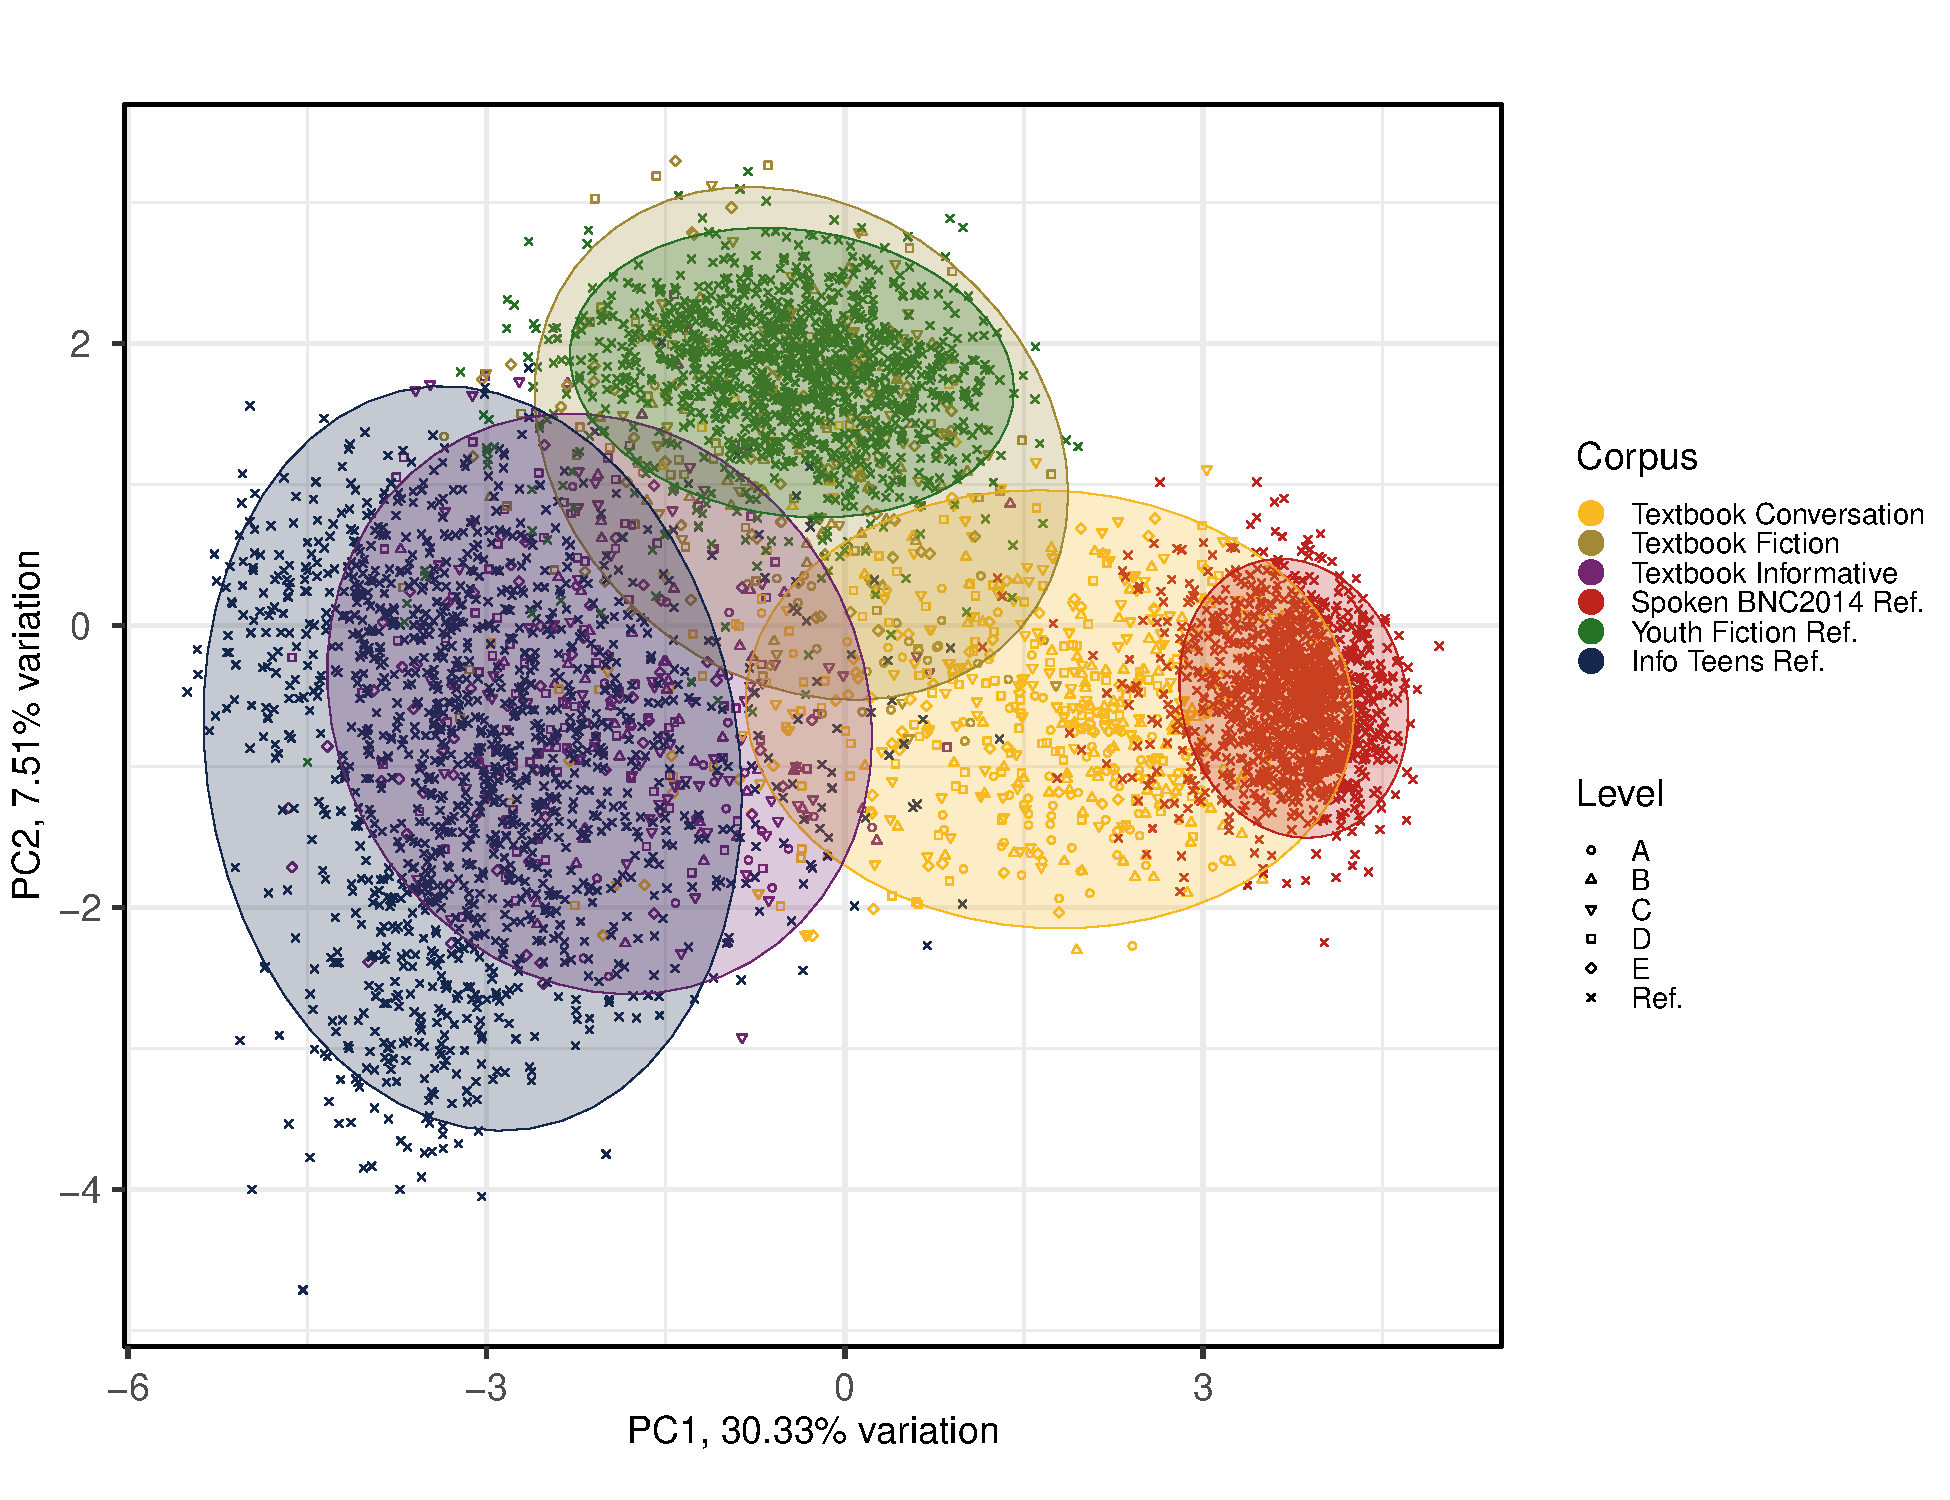
\includegraphics[keepaspectratio]{AppendixH_files/figure-pdf/PCAtools-biplots-TxB-1.pdf}}

\begin{Shaded}
\begin{Highlighting}[]
\CommentTok{\#ggsave(here("plots", "PCA\_Ref3TxB\_BiplotPC1\_PC2.svg"), width = 12, height = 8)}

\CommentTok{\# Biplots to examine components more carefully}
\NormalTok{PCAtools}\SpecialCharTok{::}\FunctionTok{biplot}\NormalTok{(p,}
                 \AttributeTok{x =} \StringTok{"PC3"}\NormalTok{,}
                 \AttributeTok{y =} \StringTok{"PC4"}\NormalTok{,}
                 \AttributeTok{lab =} \ConstantTok{NULL}\NormalTok{, }\CommentTok{\# Otherwise will try to label each data point!}
                 \AttributeTok{colby =} \StringTok{"Corpus"}\NormalTok{,}
                 \AttributeTok{pointSize =} \FloatTok{1.2}\NormalTok{,}
                 \AttributeTok{colkey =}\NormalTok{ colkey,}
                 \AttributeTok{shape =} \StringTok{"Level"}\NormalTok{,}
                 \AttributeTok{shapekey =}\NormalTok{ shapekey,}
                 \AttributeTok{xlim =} \FunctionTok{c}\NormalTok{(}\FunctionTok{min}\NormalTok{(p}\SpecialCharTok{$}\NormalTok{rotated[, }\StringTok{"PC3"}\NormalTok{]), }\FunctionTok{max}\NormalTok{(p}\SpecialCharTok{$}\NormalTok{rotated[, }\StringTok{"PC3"}\NormalTok{])),}
                 \AttributeTok{ylim =} \FunctionTok{c}\NormalTok{(}\FunctionTok{min}\NormalTok{(p}\SpecialCharTok{$}\NormalTok{rotated[, }\StringTok{"PC4"}\NormalTok{]), }\FunctionTok{max}\NormalTok{(p}\SpecialCharTok{$}\NormalTok{rotated[, }\StringTok{"PC4"}\NormalTok{])),}
                 \AttributeTok{showLoadings =} \ConstantTok{FALSE}\NormalTok{,}
                 \AttributeTok{ellipse =} \ConstantTok{TRUE}\NormalTok{,}
                 \AttributeTok{axisLabSize =} \DecValTok{18}\NormalTok{,}
                 \AttributeTok{legendPosition =} \StringTok{\textquotesingle{}right\textquotesingle{}}\NormalTok{,}
                 \AttributeTok{legendTitleSize =} \DecValTok{18}\NormalTok{,}
                 \AttributeTok{legendLabSize =} \DecValTok{14}\NormalTok{, }
                 \AttributeTok{legendIconSize =} \DecValTok{5}\NormalTok{) }\SpecialCharTok{+}
  \FunctionTok{theme}\NormalTok{(}\AttributeTok{plot.margin =} \FunctionTok{unit}\NormalTok{(}\FunctionTok{c}\NormalTok{(}\DecValTok{0}\NormalTok{,}\DecValTok{0}\NormalTok{,}\DecValTok{0}\NormalTok{,}\FloatTok{0.2}\NormalTok{), }\StringTok{"cm"}\NormalTok{))}
\end{Highlighting}
\end{Shaded}

\pandocbounded{\includegraphics[keepaspectratio]{AppendixH_files/figure-pdf/PCAtools-biplots-TxB-2.pdf}}

\begin{Shaded}
\begin{Highlighting}[]
\CommentTok{\#ggsave(here("plots", "PCA\_Ref3TxB\_BiplotPC3\_PC4.svg"), width = 12, height = 8)}
\end{Highlighting}
\end{Shaded}

The colours and corresponding ellipses can be used to visualise
different clusters and patterns. In the following, we change the colour
of the points and the ellipses to represent the texts' target
proficiency levels instead of the register, allowing for a different
interpretation of the model.

\begin{Shaded}
\begin{Highlighting}[]
\CommentTok{\# Biplot with ellipses for Level rather than Register}
\NormalTok{colkeyLevels }\OtherTok{=} \FunctionTok{c}\NormalTok{(}\AttributeTok{A=}\StringTok{"\#F9B921"}\NormalTok{, }\AttributeTok{B=}\StringTok{"\#A18A33"}\NormalTok{, }\AttributeTok{C=}\StringTok{"\#BD241E"}\NormalTok{, }\AttributeTok{D=}\StringTok{"\#722672"}\NormalTok{, }\AttributeTok{E=}\StringTok{"\#15274D"}\NormalTok{, }\StringTok{\textasciigrave{}}\AttributeTok{Ref. data}\StringTok{\textasciigrave{}}\OtherTok{=} \StringTok{"darkgrey"}\NormalTok{)}
\NormalTok{shapekeyLevels }\OtherTok{=} \FunctionTok{c}\NormalTok{(}\StringTok{\textasciigrave{}}\AttributeTok{Spoken BNC2014 Ref.}\StringTok{\textasciigrave{}}\OtherTok{=}\DecValTok{16}\NormalTok{, }\StringTok{\textasciigrave{}}\AttributeTok{Info Teens Ref.}\StringTok{\textasciigrave{}}\OtherTok{=}\DecValTok{17}\NormalTok{, }\StringTok{\textasciigrave{}}\AttributeTok{Youth Fiction Ref.}\StringTok{\textasciigrave{}}\OtherTok{=}\DecValTok{15}\NormalTok{, }\StringTok{\textasciigrave{}}\AttributeTok{Textbook Fiction}\StringTok{\textasciigrave{}}\OtherTok{=}\DecValTok{0}\NormalTok{, }\StringTok{\textasciigrave{}}\AttributeTok{Textbook Conversation}\StringTok{\textasciigrave{}}\OtherTok{=}\DecValTok{1}\NormalTok{, }\StringTok{\textasciigrave{}}\AttributeTok{Textbook Informative}\StringTok{\textasciigrave{}}\OtherTok{=}\DecValTok{2}\NormalTok{)}

\NormalTok{PCAtools}\SpecialCharTok{::}\FunctionTok{biplot}\NormalTok{(p,}
                 \AttributeTok{x =} \StringTok{"PC3"}\NormalTok{,}
                 \AttributeTok{y =} \StringTok{"PC4"}\NormalTok{,}
                 \AttributeTok{lab =} \ConstantTok{NULL}\NormalTok{, }\CommentTok{\# Otherwise will try to label each data point!}
                 \AttributeTok{colby =} \StringTok{"Level"}\NormalTok{,}
                 \AttributeTok{pointSize =} \FloatTok{1.3}\NormalTok{,}
                 \AttributeTok{colkey =}\NormalTok{ colkeyLevels,}
                 \AttributeTok{shape =} \StringTok{"Corpus"}\NormalTok{,}
                 \AttributeTok{shapekey =}\NormalTok{ shapekeyLevels,}
                 \AttributeTok{xlim =} \FunctionTok{c}\NormalTok{(}\FunctionTok{min}\NormalTok{(p}\SpecialCharTok{$}\NormalTok{rotated[, }\StringTok{"PC3"}\NormalTok{]), }\FunctionTok{max}\NormalTok{(p}\SpecialCharTok{$}\NormalTok{rotated[, }\StringTok{"PC3"}\NormalTok{])),}
                 \AttributeTok{ylim =} \FunctionTok{c}\NormalTok{(}\FunctionTok{min}\NormalTok{(p}\SpecialCharTok{$}\NormalTok{rotated[, }\StringTok{"PC4"}\NormalTok{]), }\FunctionTok{max}\NormalTok{(p}\SpecialCharTok{$}\NormalTok{rotated[, }\StringTok{"PC4"}\NormalTok{])),}
                 \AttributeTok{showLoadings =} \ConstantTok{FALSE}\NormalTok{,}
                 \AttributeTok{ellipse =} \ConstantTok{TRUE}\NormalTok{,}
                 \AttributeTok{axisLabSize =} \DecValTok{18}\NormalTok{,}
                 \AttributeTok{legendPosition =} \StringTok{\textquotesingle{}right\textquotesingle{}}\NormalTok{,}
                 \AttributeTok{legendTitleSize =} \DecValTok{18}\NormalTok{,}
                 \AttributeTok{legendLabSize =} \DecValTok{14}\NormalTok{, }
                 \AttributeTok{legendIconSize =} \DecValTok{5}\NormalTok{) }\SpecialCharTok{+}
  \FunctionTok{theme}\NormalTok{(}\AttributeTok{plot.margin =} \FunctionTok{unit}\NormalTok{(}\FunctionTok{c}\NormalTok{(}\DecValTok{0}\NormalTok{,}\DecValTok{0}\NormalTok{,}\DecValTok{0}\NormalTok{,}\FloatTok{0.2}\NormalTok{), }\StringTok{"cm"}\NormalTok{))}
\end{Highlighting}
\end{Shaded}

\pandocbounded{\includegraphics[keepaspectratio]{AppendixH_files/figure-pdf/PCAtools-biplots-TxB-Levels-1.pdf}}

\begin{Shaded}
\begin{Highlighting}[]
\CommentTok{\#ggsave(here("plots", "PCA\_Ref3TxB\_BiplotPC3\_PC4\_levels.svg"), width = 12, height = 8)}
\end{Highlighting}
\end{Shaded}

\section{Feature contributions (loadings) on each
component}\label{feature-contributions-loadings-on-each-component-1}

\begin{Shaded}
\begin{Highlighting}[]
\NormalTok{pca }\OtherTok{\textless{}{-}} \FunctionTok{prcomp}\NormalTok{(data[,}\DecValTok{9}\SpecialCharTok{:}\FunctionTok{ncol}\NormalTok{(data)], }\AttributeTok{scale.=}\ConstantTok{FALSE}\NormalTok{) }\CommentTok{\# All quantitative variables to be included in the model}

\CommentTok{\# The rotated data that represents the observations / samples is stored in rotated, while the variable loadings are stored in loadings}
\NormalTok{loadings }\OtherTok{\textless{}{-}} \FunctionTok{as.data.frame}\NormalTok{(pca}\SpecialCharTok{$}\NormalTok{rotation[,}\DecValTok{1}\SpecialCharTok{:}\DecValTok{4}\NormalTok{])}

\CommentTok{\# Table of loadings with no minimum threshold applied}
\NormalTok{loadings }\SpecialCharTok{|\textgreater{}} 
  \FunctionTok{round}\NormalTok{(}\DecValTok{2}\NormalTok{) }\SpecialCharTok{|\textgreater{}} 
  \FunctionTok{kable}\NormalTok{()}
\end{Highlighting}
\end{Shaded}

\begin{longtable}[]{@{}lrrrr@{}}
\toprule\noalign{}
& PC1 & PC2 & PC3 & PC4 \\
\midrule\noalign{}
\endhead
\bottomrule\noalign{}
\endlastfoot
ACT & -0.10 & 0.01 & -0.01 & 0.12 \\
AMP & 0.00 & -0.05 & -0.05 & 0.09 \\
ASPECT & -0.08 & 0.10 & -0.01 & 0.00 \\
AWL & -0.21 & -0.13 & -0.06 & -0.01 \\
BEMA & 0.08 & -0.24 & 0.06 & -0.02 \\
CAUSE & -0.08 & -0.12 & 0.06 & 0.14 \\
CC & -0.14 & -0.13 & -0.09 & -0.09 \\
COMM & -0.03 & 0.19 & 0.03 & 0.20 \\
CONC & -0.03 & -0.03 & -0.18 & -0.06 \\
COND & 0.08 & -0.02 & -0.17 & 0.23 \\
CONT & 0.22 & -0.05 & 0.03 & 0.00 \\
CUZ & 0.10 & -0.14 & -0.20 & -0.18 \\
DEMO & 0.15 & -0.12 & -0.08 & -0.04 \\
DMA & 0.20 & -0.09 & -0.04 & -0.16 \\
DOAUX & 0.18 & -0.02 & 0.06 & 0.00 \\
DT & 0.08 & 0.16 & -0.24 & -0.03 \\
DWNT & -0.04 & 0.10 & -0.12 & 0.09 \\
ELAB & -0.07 & -0.17 & -0.04 & 0.07 \\
EMPH & 0.17 & -0.07 & -0.09 & -0.03 \\
EX & 0.06 & -0.02 & -0.04 & 0.00 \\
EXIST & -0.13 & -0.09 & -0.05 & 0.00 \\
FPP1P & 0.08 & -0.02 & 0.09 & 0.19 \\
FPP1S & 0.17 & 0.06 & 0.06 & 0.08 \\
FPUH & 0.18 & -0.10 & -0.05 & -0.19 \\
GTO & 0.14 & 0.00 & -0.04 & 0.00 \\
HDG & 0.10 & -0.07 & -0.14 & -0.12 \\
HGOT & 0.16 & -0.05 & -0.01 & -0.11 \\
IN & -0.21 & -0.01 & -0.08 & 0.01 \\
JJAT & -0.05 & -0.13 & -0.25 & 0.07 \\
JJPR & -0.03 & -0.17 & -0.03 & 0.21 \\
LD & -0.17 & -0.16 & 0.13 & -0.04 \\
MDCA & 0.05 & -0.21 & 0.11 & 0.22 \\
MDCO & 0.00 & 0.19 & -0.15 & 0.10 \\
MDMM & -0.02 & -0.10 & -0.14 & 0.17 \\
MDNE & 0.06 & -0.02 & -0.06 & 0.22 \\
MDWO & 0.07 & 0.11 & -0.18 & 0.04 \\
MDWS & 0.06 & -0.02 & -0.01 & 0.25 \\
MENTAL & 0.11 & -0.02 & -0.05 & 0.16 \\
NCOMP & 0.00 & -0.27 & -0.05 & 0.03 \\
NN & -0.21 & -0.10 & 0.10 & -0.07 \\
OCCUR & -0.13 & -0.02 & -0.05 & -0.06 \\
PASS & -0.14 & -0.13 & -0.09 & -0.10 \\
PEAS & -0.06 & 0.12 & -0.19 & 0.12 \\
PIT & 0.15 & -0.10 & -0.15 & -0.07 \\
PLACE & 0.02 & 0.09 & 0.09 & 0.07 \\
POLITE & 0.09 & 0.00 & 0.20 & 0.11 \\
POS & 0.02 & 0.09 & 0.04 & -0.05 \\
PROG & 0.09 & 0.08 & -0.04 & 0.15 \\
QUAN & 0.17 & -0.01 & -0.16 & 0.01 \\
QUPR & 0.08 & 0.11 & -0.12 & 0.21 \\
QUTAG & 0.15 & -0.04 & -0.07 & -0.15 \\
RB & 0.14 & 0.15 & -0.18 & 0.07 \\
RP & -0.01 & 0.22 & -0.09 & 0.15 \\
SPLIT & -0.03 & -0.11 & -0.21 & 0.08 \\
SPP2 & 0.17 & -0.07 & 0.10 & 0.16 \\
STPR & 0.10 & 0.01 & 0.01 & -0.04 \\
THATD & 0.16 & -0.01 & -0.14 & -0.02 \\
THRC & -0.05 & -0.17 & -0.15 & -0.02 \\
THSC & -0.02 & -0.08 & -0.27 & 0.07 \\
TTR & -0.19 & 0.07 & -0.02 & 0.16 \\
VBD & -0.10 & 0.35 & -0.05 & -0.20 \\
VBG & -0.14 & -0.02 & -0.14 & 0.12 \\
VBN & -0.14 & -0.10 & -0.08 & -0.07 \\
VIMP & 0.01 & -0.07 & 0.21 & 0.21 \\
WHQU & 0.13 & -0.02 & 0.20 & 0.07 \\
WHSC & -0.09 & -0.10 & -0.20 & 0.05 \\
XX0 & 0.18 & 0.01 & -0.06 & 0.06 \\
YNQU & 0.18 & -0.03 & 0.14 & -0.02 \\
TPP3 & -0.05 & 0.30 & -0.04 & -0.15 \\
FQTI & -0.07 & 0.03 & 0.01 & 0.14 \\
\end{longtable}

\begin{Shaded}
\begin{Highlighting}[]
\CommentTok{\#clipr::write\_last\_clip()}
\end{Highlighting}
\end{Shaded}

\section{Graphs of features of that contribute most to each
component/dimension}\label{graphs-of-features-of-that-contribute-most-to-each-componentdimension}

Graphs of features display the features with the strongest contributions
to any two dimensions of the model of intra-textbook variation. They are
created using the \texttt{factoextra::fviz\_pca\_var} function.

\begin{Shaded}
\begin{Highlighting}[]
\NormalTok{factoextra}\SpecialCharTok{::}\FunctionTok{fviz\_pca\_var}\NormalTok{(pca,}
             \AttributeTok{axes =} \FunctionTok{c}\NormalTok{(}\DecValTok{1}\NormalTok{,}\DecValTok{2}\NormalTok{),}
             \AttributeTok{select.var =} \FunctionTok{list}\NormalTok{(}\AttributeTok{contrib =} \DecValTok{25}\NormalTok{),}
             \AttributeTok{col.var =} \StringTok{"contrib"}\NormalTok{, }\CommentTok{\# Colour by contributions to the PC}
             \AttributeTok{gradient.cols =} \FunctionTok{c}\NormalTok{(}\StringTok{"\#F9B921"}\NormalTok{, }\StringTok{"\#DB241E"}\NormalTok{, }\StringTok{"\#722672"}\NormalTok{),}
             \AttributeTok{title =} \StringTok{""}\NormalTok{,}
             \AttributeTok{repel =} \ConstantTok{TRUE}\NormalTok{, }\CommentTok{\# Try to avoid too much text overlapping}
             \AttributeTok{ggtheme =}\NormalTok{ ggthemes}\SpecialCharTok{::}\FunctionTok{theme\_few}\NormalTok{())}
\end{Highlighting}
\end{Shaded}

\pandocbounded{\includegraphics[keepaspectratio]{AppendixH_files/figure-pdf/graphs-of-variables-1.pdf}}

\begin{Shaded}
\begin{Highlighting}[]
\CommentTok{\#ggsave(here("plots", "fviz\_pca\_var\_PC1\_PC2\_Ref3Reg.svg"), width = 9, height = 7)}

\NormalTok{factoextra}\SpecialCharTok{::}\FunctionTok{fviz\_pca\_var}\NormalTok{(pca,}
             \AttributeTok{axes =} \FunctionTok{c}\NormalTok{(}\DecValTok{3}\NormalTok{,}\DecValTok{2}\NormalTok{),}
             \AttributeTok{select.var =} \FunctionTok{list}\NormalTok{(}\AttributeTok{contrib =} \DecValTok{30}\NormalTok{),}
             \AttributeTok{col.var =} \StringTok{"contrib"}\NormalTok{, }\CommentTok{\# Colour by contributions to the PC}
             \AttributeTok{gradient.cols =} \FunctionTok{c}\NormalTok{(}\StringTok{"\#F9B921"}\NormalTok{, }\StringTok{"\#DB241E"}\NormalTok{, }\StringTok{"\#722672"}\NormalTok{),}
             \AttributeTok{title =} \StringTok{""}\NormalTok{,}
             \AttributeTok{repel =} \ConstantTok{TRUE}\NormalTok{, }\CommentTok{\# Try to avoid too much text overlapping}
             \AttributeTok{ggtheme =}\NormalTok{ ggthemes}\SpecialCharTok{::}\FunctionTok{theme\_few}\NormalTok{())}
\end{Highlighting}
\end{Shaded}

\pandocbounded{\includegraphics[keepaspectratio]{AppendixH_files/figure-pdf/graphs-of-variables-2.pdf}}

\begin{Shaded}
\begin{Highlighting}[]
\CommentTok{\#ggsave(here("plots", "fviz\_pca\_var\_PC3\_PC2\_Ref3Reg.svg"), width = 9, height = 8)}

\NormalTok{factoextra}\SpecialCharTok{::}\FunctionTok{fviz\_pca\_var}\NormalTok{(pca,}
             \AttributeTok{axes =} \FunctionTok{c}\NormalTok{(}\DecValTok{3}\NormalTok{,}\DecValTok{4}\NormalTok{),}
             \AttributeTok{select.var =} \FunctionTok{list}\NormalTok{(}\AttributeTok{contrib =} \DecValTok{30}\NormalTok{),}
             \AttributeTok{col.var =} \StringTok{"contrib"}\NormalTok{, }\CommentTok{\# Colour by contributions to the PC}
             \AttributeTok{gradient.cols =} \FunctionTok{c}\NormalTok{(}\StringTok{"\#F9B921"}\NormalTok{, }\StringTok{"\#DB241E"}\NormalTok{, }\StringTok{"\#722672"}\NormalTok{),}
             \AttributeTok{title =} \StringTok{""}\NormalTok{,}
             \AttributeTok{repel =} \ConstantTok{TRUE}\NormalTok{, }\CommentTok{\# Try to avoid too much text overlapping}
             \AttributeTok{ggtheme =}\NormalTok{ ggthemes}\SpecialCharTok{::}\FunctionTok{theme\_few}\NormalTok{())}
\end{Highlighting}
\end{Shaded}

\pandocbounded{\includegraphics[keepaspectratio]{AppendixH_files/figure-pdf/graphs-of-variables-3.pdf}}

\begin{Shaded}
\begin{Highlighting}[]
\CommentTok{\#ggsave(here("plots", "fviz\_pca\_var\_PC3\_PC4\_Ref3Reg.svg"), width = 9, height = 8)}
\end{Highlighting}
\end{Shaded}

\section{Exploring feature contributions in terms of normalised
frequencies}\label{exploring-feature-contributions-in-terms-of-normalised-frequencies}

We can go back to the normalised frequencies of the individual features
to compare them across different registers and levels, e.g.,:

\begin{Shaded}
\begin{Highlighting}[]
\NormalTok{ncounts }\OtherTok{\textless{}{-}} \FunctionTok{readRDS}\NormalTok{(}\FunctionTok{here}\NormalTok{(}\StringTok{"data"}\NormalTok{, }\StringTok{"processed"}\NormalTok{, }\StringTok{"ncounts3\_3Reg.rds"}\NormalTok{))}

\NormalTok{ncounts }\SpecialCharTok{|\textgreater{}} 
  \FunctionTok{filter}\NormalTok{(Register}\SpecialCharTok{==}\StringTok{"Informative"}\NormalTok{) }\SpecialCharTok{|\textgreater{}} 
  \CommentTok{\#filter(Level \%in\% c("C", "D", "E")) |\textgreater{} }
  \FunctionTok{select}\NormalTok{(Level, VBD, PEAS) }\SpecialCharTok{|\textgreater{}} 
  \FunctionTok{group\_by}\NormalTok{(Level) }\SpecialCharTok{|\textgreater{}} 
  \FunctionTok{summarise\_if}\NormalTok{(is.numeric, mean) }\SpecialCharTok{|\textgreater{}} 
  \FunctionTok{kable}\NormalTok{(}\AttributeTok{digits=}\DecValTok{2}\NormalTok{)}
\end{Highlighting}
\end{Shaded}

\begin{longtable}[]{@{}lrr@{}}
\toprule\noalign{}
Level & VBD & PEAS \\
\midrule\noalign{}
\endhead
\bottomrule\noalign{}
\endlastfoot
A & 28.11 & 0.21 \\
B & 34.11 & 2.49 \\
C & 35.21 & 5.36 \\
D & 39.83 & 7.63 \\
E & 35.17 & 6.91 \\
Ref. & 39.73 & 4.94 \\
\end{longtable}

The following chunk produces Figure 35 which shows normalised counts of
selected features with salient loadings on PC1 in the Textbook
Informative subcorpus (Levels A to E) and the reference Info Teens
corpus (Ref.). This plots visualises the observed normalised frequencies
as they were extracted using the MFTE Perl (see Appendices C and F).

\begin{Shaded}
\begin{Highlighting}[]
\NormalTok{cols }\OtherTok{=} \FunctionTok{c}\NormalTok{(}\StringTok{"\#F9B921"}\NormalTok{, }\StringTok{"\#A18A33"}\NormalTok{, }\StringTok{"\#BD241E"}\NormalTok{, }\StringTok{"\#722672"}\NormalTok{, }\StringTok{"\#15274D"}\NormalTok{, }\StringTok{"darkgrey"}\NormalTok{)}

\NormalTok{boxfeature }\OtherTok{\textless{}{-}}\NormalTok{ ncounts }\SpecialCharTok{|\textgreater{}} 
  \FunctionTok{filter}\NormalTok{(Register}\SpecialCharTok{==}\StringTok{"Informative"}\NormalTok{) }\SpecialCharTok{|\textgreater{}} 
  \CommentTok{\#filter(Level \%in\% c("C", "D", "E")) |\textgreater{} }
  \FunctionTok{select}\NormalTok{(Level, FPP1S, SPP2, CONT, EXIST, AWL, XX0, PASS, VBN) }\SpecialCharTok{|\textgreater{}} 
  \FunctionTok{ggplot}\NormalTok{(}\FunctionTok{aes}\NormalTok{(}\AttributeTok{x =}\NormalTok{ Level, }\AttributeTok{y =}\NormalTok{ CONT, }\AttributeTok{colour =}\NormalTok{ Level, }\AttributeTok{fill =}\NormalTok{ Level)) }\SpecialCharTok{+}
  \FunctionTok{geom\_jitter}\NormalTok{(}\AttributeTok{size=}\FloatTok{0.7}\NormalTok{, }\AttributeTok{alpha=}\NormalTok{.}\DecValTok{7}\NormalTok{) }\SpecialCharTok{+}
  \FunctionTok{geom\_boxplot}\NormalTok{(}\AttributeTok{outlier.shape =} \ConstantTok{NA}\NormalTok{, }\AttributeTok{fatten =} \DecValTok{2}\NormalTok{, }\AttributeTok{fill =} \StringTok{"white"}\NormalTok{, }\AttributeTok{alpha =} \FloatTok{0.3}\NormalTok{) }\SpecialCharTok{+}
  \FunctionTok{scale\_colour\_manual}\NormalTok{(}\AttributeTok{values =}\NormalTok{ cols) }\SpecialCharTok{+}
  \FunctionTok{theme\_minimal}\NormalTok{() }\SpecialCharTok{+}
  \FunctionTok{theme}\NormalTok{(}\AttributeTok{legend.position =} \StringTok{"none"}\NormalTok{) }\SpecialCharTok{+}
  \FunctionTok{xlab}\NormalTok{(}\StringTok{""}\NormalTok{)}

\NormalTok{CONT }\OtherTok{=}\NormalTok{ boxfeature}
\NormalTok{SPP2 }\OtherTok{\textless{}{-}}\NormalTok{ boxfeature }\SpecialCharTok{+} \FunctionTok{aes}\NormalTok{(}\AttributeTok{y =}\NormalTok{ SPP2) }
\NormalTok{EXIST }\OtherTok{\textless{}{-}}\NormalTok{ boxfeature }\SpecialCharTok{+} \FunctionTok{aes}\NormalTok{(}\AttributeTok{y =}\NormalTok{ EXIST) }\SpecialCharTok{+} \FunctionTok{ylim}\NormalTok{(}\FunctionTok{c}\NormalTok{(}\DecValTok{0}\NormalTok{,}\DecValTok{25}\NormalTok{)) }\CommentTok{\# These y{-}axis limits remove individual outliers that overextend the scales and make the existing differences invisible to the naked eye. They can be removed to visualise all data points.}
\NormalTok{FFP1 }\OtherTok{\textless{}{-}}\NormalTok{ boxfeature }\SpecialCharTok{+} \FunctionTok{aes}\NormalTok{(}\AttributeTok{y =}\NormalTok{ FPP1S) }\SpecialCharTok{+} \FunctionTok{ylim}\NormalTok{(}\FunctionTok{c}\NormalTok{(}\DecValTok{0}\NormalTok{,}\DecValTok{60}\NormalTok{))  }
\NormalTok{AWL }\OtherTok{\textless{}{-}}\NormalTok{ boxfeature }\SpecialCharTok{+} \FunctionTok{aes}\NormalTok{(}\AttributeTok{y =}\NormalTok{ AWL)}
\NormalTok{XX0 }\OtherTok{\textless{}{-}}\NormalTok{ boxfeature }\SpecialCharTok{+} \FunctionTok{aes}\NormalTok{(}\AttributeTok{y =}\NormalTok{ XX0) }\SpecialCharTok{+} \FunctionTok{ylim}\NormalTok{(}\FunctionTok{c}\NormalTok{(}\DecValTok{0}\NormalTok{,}\DecValTok{25}\NormalTok{))}
\NormalTok{PASS }\OtherTok{\textless{}{-}}\NormalTok{ boxfeature }\SpecialCharTok{+} \FunctionTok{aes}\NormalTok{(}\AttributeTok{y =}\NormalTok{ PASS)}
\NormalTok{VBN }\OtherTok{\textless{}{-}}\NormalTok{ boxfeature }\SpecialCharTok{+} \FunctionTok{aes}\NormalTok{(}\AttributeTok{y =}\NormalTok{ VBN) }\SpecialCharTok{+} \FunctionTok{ylim}\NormalTok{(}\FunctionTok{c}\NormalTok{(}\DecValTok{0}\NormalTok{,}\DecValTok{40}\NormalTok{))}

\NormalTok{boxplots }\OtherTok{\textless{}{-}}\NormalTok{ gridExtra}\SpecialCharTok{::}\FunctionTok{grid.arrange}\NormalTok{(PASS, VBN, AWL, EXIST, FFP1, SPP2, CONT, XX0, }\AttributeTok{ncol=}\DecValTok{2}\NormalTok{, }\AttributeTok{nrow=}\DecValTok{4}\NormalTok{)}
\end{Highlighting}
\end{Shaded}

\pandocbounded{\includegraphics[keepaspectratio]{AppendixH_files/figure-pdf/boxplots-1.pdf}}

\begin{Shaded}
\begin{Highlighting}[]
\CommentTok{\#ggsave(here("plots", "BoxplotsInformativeFeatures.svg"), plot = boxplots, dpi = 300, width = 9, height = 11)}
\end{Highlighting}
\end{Shaded}

\section{Exploring the dimensions of the
model}\label{exploring-the-dimensions-of-the-model-1}

We begin with some descriptive statistics of the dimension scores.

\begin{Shaded}
\begin{Highlighting}[]
\CommentTok{\#data \textless{}{-} readRDS(here("data", "processed", "dataforPCA.rds")) }
\CommentTok{\#colnames(data)}
\NormalTok{pca }\OtherTok{\textless{}{-}} \FunctionTok{prcomp}\NormalTok{(data[,}\DecValTok{9}\SpecialCharTok{:}\FunctionTok{ncol}\NormalTok{(data)], }\AttributeTok{scale.=}\ConstantTok{FALSE}\NormalTok{) }\CommentTok{\# All quantitative variables}

\DocumentationTok{\#\# Access to the PCA results}
\CommentTok{\#colnames(data)}
\NormalTok{res.ind }\OtherTok{\textless{}{-}} \FunctionTok{cbind}\NormalTok{(data[,}\DecValTok{1}\SpecialCharTok{:}\DecValTok{8}\NormalTok{], }\FunctionTok{as.data.frame}\NormalTok{(pca}\SpecialCharTok{$}\NormalTok{x)[,}\DecValTok{1}\SpecialCharTok{:}\DecValTok{4}\NormalTok{])}

\DocumentationTok{\#\# Summary statistics}
\NormalTok{res.ind }\SpecialCharTok{|\textgreater{}} 
  \FunctionTok{group\_by}\NormalTok{(Subcorpus, Level) }\SpecialCharTok{|\textgreater{}} 
  \FunctionTok{summarise\_if}\NormalTok{(is.numeric, }\FunctionTok{c}\NormalTok{(}\AttributeTok{mean =}\NormalTok{ mean, }\AttributeTok{sd =}\NormalTok{ sd)) }\SpecialCharTok{|\textgreater{}} 
  \FunctionTok{kable}\NormalTok{(}\AttributeTok{digits =} \DecValTok{2}\NormalTok{)  }
\end{Highlighting}
\end{Shaded}

\begin{longtable}[]{@{}
  >{\raggedright\arraybackslash}p{(\linewidth - 22\tabcolsep) * \real{0.1964}}
  >{\raggedright\arraybackslash}p{(\linewidth - 22\tabcolsep) * \real{0.0536}}
  >{\raggedleft\arraybackslash}p{(\linewidth - 22\tabcolsep) * \real{0.0982}}
  >{\raggedleft\arraybackslash}p{(\linewidth - 22\tabcolsep) * \real{0.0804}}
  >{\raggedleft\arraybackslash}p{(\linewidth - 22\tabcolsep) * \real{0.0804}}
  >{\raggedleft\arraybackslash}p{(\linewidth - 22\tabcolsep) * \real{0.0804}}
  >{\raggedleft\arraybackslash}p{(\linewidth - 22\tabcolsep) * \real{0.0804}}
  >{\raggedleft\arraybackslash}p{(\linewidth - 22\tabcolsep) * \real{0.0804}}
  >{\raggedleft\arraybackslash}p{(\linewidth - 22\tabcolsep) * \real{0.0625}}
  >{\raggedleft\arraybackslash}p{(\linewidth - 22\tabcolsep) * \real{0.0625}}
  >{\raggedleft\arraybackslash}p{(\linewidth - 22\tabcolsep) * \real{0.0625}}
  >{\raggedleft\arraybackslash}p{(\linewidth - 22\tabcolsep) * \real{0.0625}}@{}}
\toprule\noalign{}
\begin{minipage}[b]{\linewidth}\raggedright
Subcorpus
\end{minipage} & \begin{minipage}[b]{\linewidth}\raggedright
Level
\end{minipage} & \begin{minipage}[b]{\linewidth}\raggedleft
Words\_mean
\end{minipage} & \begin{minipage}[b]{\linewidth}\raggedleft
PC1\_mean
\end{minipage} & \begin{minipage}[b]{\linewidth}\raggedleft
PC2\_mean
\end{minipage} & \begin{minipage}[b]{\linewidth}\raggedleft
PC3\_mean
\end{minipage} & \begin{minipage}[b]{\linewidth}\raggedleft
PC4\_mean
\end{minipage} & \begin{minipage}[b]{\linewidth}\raggedleft
Words\_sd
\end{minipage} & \begin{minipage}[b]{\linewidth}\raggedleft
PC1\_sd
\end{minipage} & \begin{minipage}[b]{\linewidth}\raggedleft
PC2\_sd
\end{minipage} & \begin{minipage}[b]{\linewidth}\raggedleft
PC3\_sd
\end{minipage} & \begin{minipage}[b]{\linewidth}\raggedleft
PC4\_sd
\end{minipage} \\
\midrule\noalign{}
\endhead
\bottomrule\noalign{}
\endlastfoot
Textbook Conversation & A & 813.02 & 1.91 & -1.02 & 3.49 & -0.17 &
154.57 & 0.89 & 0.60 & 1.03 & 0.73 \\
Textbook Conversation & B & 819.48 & 2.11 & -0.64 & 2.33 & 0.39 & 218.88
& 0.91 & 0.69 & 1.04 & 0.79 \\
Textbook Conversation & C & 823.69 & 1.59 & -0.38 & 1.39 & 0.75 & 279.14
& 1.20 & 0.73 & 1.04 & 0.79 \\
Textbook Conversation & D & 797.85 & 1.09 & -0.43 & 0.79 & 0.91 & 187.98
& 1.45 & 0.72 & 1.26 & 0.79 \\
Textbook Conversation & E & 1132.79 & 1.03 & -0.61 & 0.86 & 1.09 &
569.85 & 1.30 & 0.78 & 0.88 & 0.62 \\
Textbook Fiction & A & 886.00 & 0.13 & 0.22 & 2.74 & -0.27 & 242.78 &
0.97 & 0.69 & 0.90 & 0.81 \\
Textbook Fiction & B & 864.16 & -0.21 & 1.34 & 1.73 & -0.29 & 222.44 &
0.79 & 0.62 & 0.73 & 0.53 \\
Textbook Fiction & C & 854.21 & -0.27 & 1.63 & 0.76 & 0.12 & 198.21 &
0.89 & 0.78 & 0.96 & 0.63 \\
Textbook Fiction & D & 801.78 & -0.84 & 1.38 & 0.26 & 0.15 & 196.33 &
1.15 & 0.79 & 0.83 & 0.59 \\
Textbook Fiction & E & 853.26 & -0.65 & 1.27 & 0.26 & 0.20 & 195.97 &
1.10 & 0.75 & 0.92 & 0.57 \\
Textbook Informative & A & 851.71 & -1.46 & -0.96 & 1.86 & -0.70 &
199.77 & 0.82 & 0.86 & 0.69 & 0.85 \\
Textbook Informative & B & 844.03 & -1.63 & -0.50 & 1.23 & -0.27 &
182.83 & 0.92 & 1.03 & 0.80 & 1.08 \\
Textbook Informative & C & 838.90 & -1.87 & -0.54 & 0.25 & 0.14 & 160.21
& 1.09 & 0.98 & 0.93 & 1.06 \\
Textbook Informative & D & 847.65 & -2.24 & -0.32 & -0.15 & 0.13 &
179.25 & 0.95 & 0.92 & 0.95 & 0.83 \\
Textbook Informative & E & 823.23 & -2.57 & -0.66 & -0.28 & 0.37 &
180.39 & 0.99 & 0.90 & 0.79 & 0.82 \\
Spoken BNC2014 Ref. & Ref. & 10637.74 & 3.71 & -0.52 & -0.64 & -0.53 &
8974.14 & 0.49 & 0.47 & 0.76 & 0.52 \\
Youth Fiction Ref. & Ref. & 5944.78 & -0.49 & 1.75 & -0.21 & 0.41 &
198.64 & 0.90 & 0.52 & 0.88 & 0.52 \\
Info Teens Ref. & Ref. & 805.41 & -3.06 & -0.96 & -0.23 & -0.15 & 193.31
& 1.09 & 1.19 & 0.88 & 1.19 \\
\end{longtable}

\begin{Shaded}
\begin{Highlighting}[]
\NormalTok{res.ind }\OtherTok{\textless{}{-}}\NormalTok{ res.ind }\SpecialCharTok{|\textgreater{}} 
  \FunctionTok{mutate}\NormalTok{(}\AttributeTok{Subsubcorpus =} \FunctionTok{paste}\NormalTok{(Corpus, Register, }\AttributeTok{sep =} \StringTok{"\_"}\NormalTok{)) }\SpecialCharTok{|\textgreater{}} 
  \FunctionTok{mutate}\NormalTok{(}\AttributeTok{Subsubcorpus =} \FunctionTok{as.factor}\NormalTok{(Subsubcorpus))}
  
\NormalTok{res.ind }\SpecialCharTok{|\textgreater{}} 
  \FunctionTok{select}\NormalTok{(PC1, PC2, PC3, PC4, Subsubcorpus) }\SpecialCharTok{|\textgreater{}} 
  \FunctionTok{tbl\_summary}\NormalTok{(}\AttributeTok{by =}\NormalTok{ Subsubcorpus,}
              \AttributeTok{digits =} \FunctionTok{list}\NormalTok{(}\FunctionTok{all\_continuous}\NormalTok{() }\SpecialCharTok{\textasciitilde{}} \FunctionTok{c}\NormalTok{(}\DecValTok{2}\NormalTok{, }\DecValTok{2}\NormalTok{)),}
              \AttributeTok{statistic =} \FunctionTok{all\_continuous}\NormalTok{() }\SpecialCharTok{\textasciitilde{}}  \StringTok{"\{mean\} (\{sd\})"}\NormalTok{)}
\end{Highlighting}
\end{Shaded}

\begin{longtable}[]{@{}
  >{\raggedright\arraybackslash}p{(\linewidth - 12\tabcolsep) * \real{0.0696}}
  >{\centering\arraybackslash}p{(\linewidth - 12\tabcolsep) * \real{0.1685}}
  >{\centering\arraybackslash}p{(\linewidth - 12\tabcolsep) * \real{0.1612}}
  >{\centering\arraybackslash}p{(\linewidth - 12\tabcolsep) * \real{0.1612}}
  >{\centering\arraybackslash}p{(\linewidth - 12\tabcolsep) * \real{0.1429}}
  >{\centering\arraybackslash}p{(\linewidth - 12\tabcolsep) * \real{0.1575}}
  >{\centering\arraybackslash}p{(\linewidth - 12\tabcolsep) * \real{0.1392}}@{}}
\toprule\noalign{}
\begin{minipage}[b]{\linewidth}\raggedright
\textbf{Characteristic}
\end{minipage} & \begin{minipage}[b]{\linewidth}\centering
\textbf{Informative.Teens\_Informative}, N = 1,337
\end{minipage} & \begin{minipage}[b]{\linewidth}\centering
\textbf{Spoken.BNC2014\_Conversation}, N = 1,250
\end{minipage} & \begin{minipage}[b]{\linewidth}\centering
\textbf{Textbook.English\_Conversation}, N = 565
\end{minipage} & \begin{minipage}[b]{\linewidth}\centering
\textbf{Textbook.English\_Fiction}, N = 285
\end{minipage} & \begin{minipage}[b]{\linewidth}\centering
\textbf{Textbook.English\_Informative}, N = 352
\end{minipage} & \begin{minipage}[b]{\linewidth}\centering
\textbf{Youth.Fiction\_Fiction}, N = 1,191
\end{minipage} \\
\midrule\noalign{}
\endhead
\bottomrule\noalign{}
\endlastfoot
PC1 & -3.06 (1.09) & 3.71 (0.49) & 1.56 (1.25) & -0.43 (1.05) & -2.05
(1.04) & -0.49 (0.90) \\
PC2 & -0.96 (1.19) & -0.52 (0.47) & -0.57 (0.74) & 1.25 (0.84) & -0.52
(0.96) & 1.75 (0.52) \\
PC3 & -0.23 (0.88) & -0.64 (0.76) & 1.71 (1.43) & 0.96 (1.22) & 0.31
(1.10) & -0.21 (0.88) \\
PC4 & -0.15 (1.19) & -0.53 (0.52) & 0.61 (0.86) & 0.02 (0.64) & 0.05
(0.98) & 0.41 (0.52) \\
\end{longtable}

\begin{Shaded}
\begin{Highlighting}[]
\NormalTok{res.ind }\SpecialCharTok{|\textgreater{}} 
  \FunctionTok{select}\NormalTok{(Register, Level, PC4) }\SpecialCharTok{|\textgreater{}} 
  \FunctionTok{group\_by}\NormalTok{(Register, Level) }\SpecialCharTok{|\textgreater{}} 
  \FunctionTok{summarise\_if}\NormalTok{(is.numeric, }\FunctionTok{c}\NormalTok{(}\AttributeTok{Median =}\NormalTok{ median, }\AttributeTok{MAD =}\NormalTok{ mad)) }\SpecialCharTok{|\textgreater{}} 
  \FunctionTok{kable}\NormalTok{(}\AttributeTok{digits =} \DecValTok{2}\NormalTok{)  }
\end{Highlighting}
\end{Shaded}

\begin{longtable}[]{@{}llrr@{}}
\toprule\noalign{}
Register & Level & Median & MAD \\
\midrule\noalign{}
\endhead
\bottomrule\noalign{}
\endlastfoot
Conversation & A & -0.07 & 0.68 \\
Conversation & B & 0.42 & 0.80 \\
Conversation & C & 0.73 & 0.80 \\
Conversation & D & 0.86 & 0.70 \\
Conversation & E & 1.09 & 0.61 \\
Conversation & Ref. & -0.54 & 0.52 \\
Fiction & A & -0.38 & 0.75 \\
Fiction & B & -0.39 & 0.53 \\
Fiction & C & 0.13 & 0.67 \\
Fiction & D & 0.01 & 0.54 \\
Fiction & E & 0.12 & 0.67 \\
Fiction & Ref. & 0.40 & 0.50 \\
Informative & A & -0.71 & 0.82 \\
Informative & B & -0.37 & 1.10 \\
Informative & C & 0.07 & 1.09 \\
Informative & D & 0.04 & 0.79 \\
Informative & E & 0.37 & 0.57 \\
Informative & Ref. & -0.08 & 1.21 \\
\end{longtable}

The following chunk can be used to search for example texts that are
located in specific areas of the biplots. For example, we can search for
texts that have high scores on Dim3 and low ones on Dim2 to proceed with
a qualitative comparison and analysis of these texts.

\begin{Shaded}
\begin{Highlighting}[]
\CommentTok{\# Search for example texts to illustrate results}
\NormalTok{res.ind }\SpecialCharTok{|\textgreater{}} 
  \FunctionTok{filter}\NormalTok{(PC3 }\SpecialCharTok{\textgreater{}} \DecValTok{2} \SpecialCharTok{\&}\NormalTok{ PC2 }\SpecialCharTok{\textless{}} \SpecialCharTok{{-}}\DecValTok{2}\NormalTok{) }\SpecialCharTok{|\textgreater{}} 
  \CommentTok{\#filter(Register=="Conversation") |\textgreater{} }
  \CommentTok{\#filter(Level == "B") |\textgreater{} }
  \CommentTok{\#filter(PC1 \textgreater{} 4.7) |\textgreater{} }
  \FunctionTok{select}\NormalTok{(Filename, PC1, PC2, PC3) }\SpecialCharTok{|\textgreater{}} 
  \FunctionTok{kable}\NormalTok{(}\AttributeTok{digits=}\DecValTok{2}\NormalTok{)}
\end{Highlighting}
\end{Shaded}

\begin{longtable}[]{@{}lrrr@{}}
\toprule\noalign{}
Filename & PC1 & PC2 & PC3 \\
\midrule\noalign{}
\endhead
\bottomrule\noalign{}
\endlastfoot
NGL\_1\_Spoken\_0002.txt & 2.41 & -2.27 & 4.36 \\
HT\_5\_ELF\_Spoken\_0003.txt & 1.94 & -2.30 & 3.49 \\
HT\_6\_Informative\_0001.txt & -2.19 & -2.36 & 3.11 \\
Science\_Tech\_Kinds\_NZ\_10383721\_typesofrobots.txt & -3.09 & -2.62 &
2.24 \\
History\_Kids\_BBC\_10402894\_go\_furthers.txt & -4.26 & -2.07 & 2.08 \\
\end{longtable}

\section{Raincloud plots visualising dimension
scores}\label{raincloud-plots-visualising-dimension-scores}

\begin{Shaded}
\begin{Highlighting}[]
\NormalTok{res.ind}\SpecialCharTok{$}\NormalTok{Subcorpus }\OtherTok{\textless{}{-}} \FunctionTok{fct\_relevel}\NormalTok{(res.ind}\SpecialCharTok{$}\NormalTok{Subcorpus, }\StringTok{"Spoken BNC2014 Ref."}\NormalTok{, }\StringTok{"Textbook Conversation"}\NormalTok{, }\StringTok{"Youth Fiction Ref."}\NormalTok{, }\StringTok{"Textbook Fiction"}\NormalTok{, }\StringTok{"Info Teens Ref."}\NormalTok{, }\StringTok{"Textbook Informative"}\NormalTok{)}

\CommentTok{\# colours \textless{}{-} suf\_palette(name = "london", n = 6, type = "continuous")}
\CommentTok{\# colours2 \textless{}{-} suf\_palette(name = "classic", n = 5, type = "continuous")}
\CommentTok{\# colours \textless{}{-} c(colours, colours2[c(2:4)]) \# Nine colours range}
\CommentTok{\# palette \textless{}{-} colours[c(1,5,6,2,3,8,7,4,9)] \# Good order for PCA}
\CommentTok{\# colours \textless{}{-} palette[c(1,8,9,2,7,3)]}

\CommentTok{\# This translates as:}
\NormalTok{palette }\OtherTok{\textless{}{-}} \FunctionTok{c}\NormalTok{(}\StringTok{"\#BD241E"}\NormalTok{, }\StringTok{"\#A18A33"}\NormalTok{, }\StringTok{"\#15274D"}\NormalTok{, }\StringTok{"\#D54E1E"}\NormalTok{, }\StringTok{"\#EA7E1E"}\NormalTok{, }\StringTok{"\#4C4C4C"}\NormalTok{, }\StringTok{"\#722672"}\NormalTok{, }\StringTok{"\#F9B921"}\NormalTok{, }\StringTok{"\#267226"}\NormalTok{)}
\NormalTok{colours }\OtherTok{\textless{}{-}} \FunctionTok{c}\NormalTok{(}\StringTok{"\#BD241E"}\NormalTok{, }\StringTok{"\#F9B921"}\NormalTok{, }\StringTok{"\#267226"}\NormalTok{, }\StringTok{"\#A18A33"}\NormalTok{, }\StringTok{"\#722672"}\NormalTok{,}\StringTok{"\#15274D"}\NormalTok{)}

\NormalTok{raincloud }\OtherTok{\textless{}{-}} \ControlFlowTok{function}\NormalTok{(data, pc\_var, from, to) \{}
  \CommentTok{\# Calculate the y{-}coordinates for the annotate() functions based on the bottom end of the y{-}axis (\textquotesingle{}from\textquotesingle{} argument)}
\NormalTok{  offset }\OtherTok{\textless{}{-}}\NormalTok{ from }\SpecialCharTok{+} \DecValTok{7}
\NormalTok{  p }\OtherTok{\textless{}{-}} \FunctionTok{ggplot}\NormalTok{(data, }\FunctionTok{aes}\NormalTok{(}\AttributeTok{x=}\NormalTok{Subcorpus, }\AttributeTok{y=}\NormalTok{.data[[pc\_var]], }\AttributeTok{fill =}\NormalTok{ Subcorpus, }\AttributeTok{colour =}\NormalTok{ Subcorpus))}\SpecialCharTok{+}
    \FunctionTok{geom\_flat\_violin}\NormalTok{(}\AttributeTok{position =} \FunctionTok{position\_nudge}\NormalTok{(}\AttributeTok{x =}\NormalTok{ .}\DecValTok{25}\NormalTok{, }\AttributeTok{y =} \DecValTok{0}\NormalTok{),}\AttributeTok{adjust =} \DecValTok{2}\NormalTok{, }\AttributeTok{trim =} \ConstantTok{FALSE}\NormalTok{)}\SpecialCharTok{+}
    \FunctionTok{geom\_point}\NormalTok{(}\AttributeTok{position =} \FunctionTok{position\_jitter}\NormalTok{(}\AttributeTok{width =}\NormalTok{ .}\DecValTok{15}\NormalTok{), }\AttributeTok{size =}\NormalTok{ .}\DecValTok{25}\NormalTok{)}\SpecialCharTok{+}
    \FunctionTok{geom\_boxplot}\NormalTok{(}\FunctionTok{aes}\NormalTok{(}\AttributeTok{x =} \FunctionTok{as.numeric}\NormalTok{(Subcorpus)}\SpecialCharTok{+}\FloatTok{0.25}\NormalTok{, }\AttributeTok{y =}\NormalTok{ .data[[pc\_var]]), }\AttributeTok{outlier.shape =} \ConstantTok{NA}\NormalTok{, }\AttributeTok{alpha =} \FloatTok{0.3}\NormalTok{, }\AttributeTok{width =}\NormalTok{ .}\DecValTok{15}\NormalTok{, }\AttributeTok{colour =} \StringTok{"BLACK"}\NormalTok{) }\SpecialCharTok{+}
    \FunctionTok{ylab}\NormalTok{(pc\_var)}\SpecialCharTok{+}
    \FunctionTok{theme\_cowplot}\NormalTok{()}\SpecialCharTok{+}
    \FunctionTok{theme}\NormalTok{(}\AttributeTok{axis.title.x=}\FunctionTok{element\_blank}\NormalTok{())}\SpecialCharTok{+}
    \FunctionTok{guides}\NormalTok{(}\AttributeTok{fill =} \StringTok{"none"}\NormalTok{, }\AttributeTok{colour =} \StringTok{"none"}\NormalTok{) }\SpecialCharTok{+}
    \FunctionTok{scale\_colour\_manual}\NormalTok{(}\AttributeTok{values =}\NormalTok{ colours)}\SpecialCharTok{+}
    \FunctionTok{scale\_fill\_manual}\NormalTok{(}\AttributeTok{values =}\NormalTok{ colours) }\SpecialCharTok{+}
    \FunctionTok{annotate}\NormalTok{(}\AttributeTok{geom =} \StringTok{"text"}\NormalTok{, }\AttributeTok{x =} \FloatTok{1.5}\NormalTok{, }\AttributeTok{y =} \SpecialCharTok{{-}}\DecValTok{7} \SpecialCharTok{+}\NormalTok{ offset, }\AttributeTok{label =} \StringTok{"Conversation"}\NormalTok{, }\AttributeTok{size =} \DecValTok{5}\NormalTok{) }\SpecialCharTok{+}
    \FunctionTok{annotate}\NormalTok{(}\AttributeTok{geom =} \StringTok{"segment"}\NormalTok{, }\AttributeTok{x =} \FloatTok{0.7}\NormalTok{, }\AttributeTok{xend =} \FloatTok{2.5}\NormalTok{, }\AttributeTok{y =} \SpecialCharTok{{-}}\FloatTok{6.5} \SpecialCharTok{+}\NormalTok{ offset, }\AttributeTok{yend =} \SpecialCharTok{{-}}\FloatTok{6.5} \SpecialCharTok{+}\NormalTok{ offset) }\SpecialCharTok{+}
    \FunctionTok{annotate}\NormalTok{(}\AttributeTok{geom =} \StringTok{"text"}\NormalTok{, }\AttributeTok{x =} \FloatTok{3.5}\NormalTok{, }\AttributeTok{y =} \SpecialCharTok{{-}}\DecValTok{7} \SpecialCharTok{+}\NormalTok{ offset, }\AttributeTok{label =} \StringTok{"Fiction"}\NormalTok{, }\AttributeTok{size =} \DecValTok{5}\NormalTok{) }\SpecialCharTok{+}
    \FunctionTok{annotate}\NormalTok{(}\AttributeTok{geom =} \StringTok{"segment"}\NormalTok{, }\AttributeTok{x =} \FloatTok{2.7}\NormalTok{, }\AttributeTok{xend =} \FloatTok{4.5}\NormalTok{, }\AttributeTok{y =} \SpecialCharTok{{-}}\FloatTok{6.5} \SpecialCharTok{+}\NormalTok{ offset, }\AttributeTok{yend =} \SpecialCharTok{{-}}\FloatTok{6.5} \SpecialCharTok{+}\NormalTok{ offset) }\SpecialCharTok{+}
    \FunctionTok{annotate}\NormalTok{(}\AttributeTok{geom =} \StringTok{"text"}\NormalTok{, }\AttributeTok{x =} \FloatTok{5.7}\NormalTok{, }\AttributeTok{y =} \SpecialCharTok{{-}}\DecValTok{7} \SpecialCharTok{+}\NormalTok{ offset, }\AttributeTok{label =} \StringTok{"Informative"}\NormalTok{, }\AttributeTok{size =} \DecValTok{5}\NormalTok{) }\SpecialCharTok{+}
    \FunctionTok{annotate}\NormalTok{(}\AttributeTok{geom =} \StringTok{"segment"}\NormalTok{, }\AttributeTok{x =} \FloatTok{4.7}\NormalTok{, }\AttributeTok{xend =} \FloatTok{6.5}\NormalTok{, }\AttributeTok{y =} \SpecialCharTok{{-}}\FloatTok{6.5} \SpecialCharTok{+}\NormalTok{ offset, }\AttributeTok{yend =} \SpecialCharTok{{-}}\FloatTok{6.5} \SpecialCharTok{+}\NormalTok{ offset) }\SpecialCharTok{+}
    \FunctionTok{scale\_x\_discrete}\NormalTok{(}\AttributeTok{labels=}\FunctionTok{rep}\NormalTok{(}\FunctionTok{c}\NormalTok{(}\StringTok{"Reference"}\NormalTok{, }\StringTok{"Textbook"}\NormalTok{), }\DecValTok{3}\NormalTok{))}\SpecialCharTok{+}
    \FunctionTok{scale\_y\_continuous}\NormalTok{(}\AttributeTok{sec.axis =} \FunctionTok{dup\_axis}\NormalTok{(}\AttributeTok{name=}\ConstantTok{NULL}\NormalTok{), }\AttributeTok{breaks =} \FunctionTok{seq}\NormalTok{(}\AttributeTok{from =}\NormalTok{ from, }\AttributeTok{to =}\NormalTok{ to, }\AttributeTok{by =} \DecValTok{1}\NormalTok{))}
  \FunctionTok{return}\NormalTok{(p)}
\NormalTok{\}}

\FunctionTok{raincloud}\NormalTok{(res.ind, }\StringTok{"PC1"}\NormalTok{, }\SpecialCharTok{{-}}\DecValTok{7}\NormalTok{, }\DecValTok{5}\NormalTok{)}
\end{Highlighting}
\end{Shaded}

\pandocbounded{\includegraphics[keepaspectratio]{AppendixH_files/figure-pdf/rainplotsDim1-1.pdf}}

\begin{Shaded}
\begin{Highlighting}[]
\CommentTok{\#ggsave(here("plots", "PC1\_3RegComparison.svg"), width = 13, height = 8)}
\CommentTok{\#ggsave(here("plots", "PC1\_3RegComparison.png"), width = 20, height = 15, units = "cm", dpi = 300)}
\end{Highlighting}
\end{Shaded}

\pandocbounded{\includegraphics[keepaspectratio]{AppendixH_files/figure-pdf/rainplotsDim2-1.pdf}}

\pandocbounded{\includegraphics[keepaspectratio]{AppendixH_files/figure-pdf/rainplotsDim3-1.pdf}}

\pandocbounded{\includegraphics[keepaspectratio]{AppendixH_files/figure-pdf/rainplotsDim4-1.pdf}}

\section{Computing mixed-effects models of the dimension
scores}\label{computing-mixed-effects-models-of-the-dimension-scores-1}

\subsection{Data preparation}\label{data-preparation}

In this chunk, we add a \texttt{Source} variable to be used as a random
effect variable in the following mixed-effects models (see 5.3.8 for
details).

\begin{Shaded}
\begin{Highlighting}[]
\NormalTok{res.ind }\OtherTok{\textless{}{-}}\NormalTok{ res.ind }\SpecialCharTok{|\textgreater{}} 
  \FunctionTok{mutate}\NormalTok{(}\AttributeTok{Source =} \FunctionTok{case\_when}\NormalTok{(}
\NormalTok{  Corpus}\SpecialCharTok{==}\StringTok{"Youth.Fiction"} \SpecialCharTok{\textasciitilde{}} \FunctionTok{paste}\NormalTok{(}\StringTok{"Book"}\NormalTok{, }\FunctionTok{str\_extract}\NormalTok{(Filename, }\StringTok{"[0{-}9]\{1,3\}"}\NormalTok{), }\AttributeTok{sep =} \StringTok{""}\NormalTok{),}
\NormalTok{  Corpus}\SpecialCharTok{==}\StringTok{"Spoken.BNC2014"} \SpecialCharTok{\textasciitilde{}} \StringTok{"Spoken.BNC2014"}\NormalTok{,}
\NormalTok{  Corpus}\SpecialCharTok{==}\StringTok{"Textbook.English"} \SpecialCharTok{\textasciitilde{}} \FunctionTok{as.character}\NormalTok{(Series),}
\NormalTok{  Corpus}\SpecialCharTok{==}\StringTok{"Informative.Teens"} \SpecialCharTok{\textasciitilde{}} \FunctionTok{str\_extract}\NormalTok{(Filename, }\StringTok{"BBC|Science\_Tech"}\NormalTok{),}
  \ConstantTok{TRUE} \SpecialCharTok{\textasciitilde{}} \StringTok{"NA"}\NormalTok{)) }\SpecialCharTok{|\textgreater{}} 
  \FunctionTok{mutate}\NormalTok{(}\AttributeTok{Source =} \FunctionTok{case\_when}\NormalTok{(}
\NormalTok{  Corpus}\SpecialCharTok{==}\StringTok{"Informative.Teens"} \SpecialCharTok{\&} \FunctionTok{is.na}\NormalTok{(Source) }\SpecialCharTok{\textasciitilde{}} \FunctionTok{str\_remove}\NormalTok{(Filename, }\StringTok{"\_.*"}\NormalTok{),}
  \ConstantTok{TRUE} \SpecialCharTok{\textasciitilde{}} \FunctionTok{as.character}\NormalTok{(Source))) }\SpecialCharTok{|\textgreater{}} 
  \FunctionTok{mutate}\NormalTok{(}\AttributeTok{Source =} \FunctionTok{as.factor}\NormalTok{(Source)) }\SpecialCharTok{|\textgreater{}} 
  \FunctionTok{mutate}\NormalTok{(}\AttributeTok{Corpus =} \FunctionTok{case\_when}\NormalTok{(}
\NormalTok{    Corpus}\SpecialCharTok{==}\StringTok{"Textbook.English"} \SpecialCharTok{\textasciitilde{}} \StringTok{"Textbook"}\NormalTok{,}
\NormalTok{    Corpus}\SpecialCharTok{==}\StringTok{"Informative.Teens"} \SpecialCharTok{\textasciitilde{}} \StringTok{"Reference"}\NormalTok{,}
\NormalTok{    Corpus}\SpecialCharTok{==}\StringTok{"Spoken.BNC2014"} \SpecialCharTok{\textasciitilde{}} \StringTok{"Reference"}\NormalTok{,}
\NormalTok{    Corpus}\SpecialCharTok{==}\StringTok{"Youth.Fiction"} \SpecialCharTok{\textasciitilde{}} \StringTok{"Reference"}
\NormalTok{  )) }\SpecialCharTok{|\textgreater{}} 
  \FunctionTok{mutate}\NormalTok{(}\AttributeTok{Corpus =} \FunctionTok{as.factor}\NormalTok{(Corpus))}

\CommentTok{\# Change the reference levels to theoretically more meaningful levels and one that is better populated (see, e.g., https://stats.stackexchange.com/questions/430770/in{-}a{-}multilevel{-}linear{-}regression{-}how{-}does{-}the{-}reference{-}level{-}affect{-}other{-}lev)}
\CommentTok{\# summary(res.ind$Corpus)}
\NormalTok{res.ind}\SpecialCharTok{$}\NormalTok{Corpus }\OtherTok{\textless{}{-}} \FunctionTok{relevel}\NormalTok{(res.ind}\SpecialCharTok{$}\NormalTok{Corpus, }\StringTok{"Reference"}\NormalTok{)}

\CommentTok{\# summary(res.ind$Subcorpus)}
\NormalTok{res.ind}\SpecialCharTok{$}\NormalTok{Subcorpus }\OtherTok{\textless{}{-}} \FunctionTok{factor}\NormalTok{(res.ind}\SpecialCharTok{$}\NormalTok{Subcorpus, }\AttributeTok{levels =} \FunctionTok{c}\NormalTok{(}\StringTok{"Spoken BNC2014 Ref."}\NormalTok{, }\StringTok{"Textbook Conversation"}\NormalTok{, }\StringTok{"Youth Fiction Ref."}\NormalTok{, }\StringTok{"Textbook Fiction"}\NormalTok{, }\StringTok{"Info Teens Ref."}\NormalTok{, }\StringTok{"Textbook Informative"}\NormalTok{))}

\CommentTok{\# summary(res.ind$Level)}
\NormalTok{res.ind}\SpecialCharTok{$}\NormalTok{Level }\OtherTok{\textless{}{-}} \FunctionTok{relevel}\NormalTok{(res.ind}\SpecialCharTok{$}\NormalTok{Level, }\StringTok{"Ref."}\NormalTok{)}
\end{Highlighting}
\end{Shaded}

\subsection{Dimension 1: `Spontaneous interactional vs.~Edited
informational'}\label{dimension-1-spontaneous-interactional-vs.-edited-informational}

We first compare various models and then present a tabular summary of
the best-fitting one.

\begin{Shaded}
\begin{Highlighting}[]
\NormalTok{md\_source }\OtherTok{\textless{}{-}} \FunctionTok{lmer}\NormalTok{(PC1 }\SpecialCharTok{\textasciitilde{}} \DecValTok{1} \SpecialCharTok{+}\NormalTok{ (Register}\SpecialCharTok{|}\NormalTok{Source), res.ind, }\AttributeTok{REML =} \ConstantTok{FALSE}\NormalTok{) }
\NormalTok{md\_corpus }\OtherTok{\textless{}{-}} \FunctionTok{update}\NormalTok{(md\_source, .}\SpecialCharTok{\textasciitilde{}}\NormalTok{. }\SpecialCharTok{+}\NormalTok{ Level) }\CommentTok{\# Failed to converge}
\NormalTok{md\_register }\OtherTok{\textless{}{-}} \FunctionTok{update}\NormalTok{(md\_source, . }\SpecialCharTok{\textasciitilde{}}\NormalTok{ . }\SpecialCharTok{+}\NormalTok{ Register)}
\NormalTok{md\_both }\OtherTok{\textless{}{-}} \FunctionTok{update}\NormalTok{(md\_corpus, .}\SpecialCharTok{\textasciitilde{}}\NormalTok{. }\SpecialCharTok{+}\NormalTok{ Register)}
\NormalTok{md\_interaction }\OtherTok{\textless{}{-}} \FunctionTok{update}\NormalTok{(md\_both, . }\SpecialCharTok{\textasciitilde{}}\NormalTok{ . }\SpecialCharTok{+}\NormalTok{ Level}\SpecialCharTok{:}\NormalTok{Register)}

\FunctionTok{anova}\NormalTok{(md\_source, md\_corpus, md\_register, md\_both, md\_interaction)}
\end{Highlighting}
\end{Shaded}

\begin{verbatim}
Data: res.ind
Models:
md_source: PC1 ~ 1 + (Register | Source)
md_register: PC1 ~ (Register | Source) + Register
md_corpus: PC1 ~ (Register | Source) + Level
md_both: PC1 ~ (Register | Source) + Level + Register
md_interaction: PC1 ~ (Register | Source) + Level + Register + Level:Register
               npar   AIC   BIC  logLik deviance   Chisq Df Pr(>Chisq)    
md_source         8 12421 12473 -6202.5    12405                          
md_register      10 12357 12422 -6168.4    12337  68.106  2  1.625e-15 ***
md_corpus        13 12181 12266 -6077.5    12155 181.996  3  < 2.2e-16 ***
md_both          15 12117 12215 -6043.5    12087  67.843  2  1.854e-15 ***
md_interaction   25 12098 12261 -6024.0    12048  39.104 10  2.435e-05 ***
---
Signif. codes:  0 '***' 0.001 '**' 0.01 '*' 0.05 '.' 0.1 ' ' 1
\end{verbatim}

\begin{Shaded}
\begin{Highlighting}[]
\NormalTok{md\_interaction }\OtherTok{\textless{}{-}} \FunctionTok{lmer}\NormalTok{(PC1 }\SpecialCharTok{\textasciitilde{}}\NormalTok{ Level }\SpecialCharTok{+}\NormalTok{ Register }\SpecialCharTok{+}\NormalTok{ Level}\SpecialCharTok{*}\NormalTok{Register }\SpecialCharTok{+}\NormalTok{ (Register}\SpecialCharTok{|}\NormalTok{Source), res.ind, }\AttributeTok{REML =} \ConstantTok{FALSE}\NormalTok{) }

\FunctionTok{tab\_model}\NormalTok{(md\_interaction, }\AttributeTok{wrap.labels =} \DecValTok{200}\NormalTok{) }\CommentTok{\# R2 = 0.870 / 0.923}
\end{Highlighting}
\end{Shaded}

Its estimated coefficients are visualised in the plot below.

\begin{Shaded}
\begin{Highlighting}[]
\CommentTok{\# Tweak plot aesthetics with: https://cran.r{-}project.org/web/packages/sjPlot/vignettes/custplot.html}
\CommentTok{\# Colour customisation trick from: https://stackoverflow.com/questions/55598920/different{-}line{-}colors{-}in{-}forest{-}plot{-}output{-}from{-}sjplot{-}r{-}package}

\FunctionTok{plot\_model}\NormalTok{(md\_interaction, }
           \CommentTok{\#type = "re", \# Option to visualise random effects }
           \AttributeTok{show.intercept =} \ConstantTok{TRUE}\NormalTok{,}
           \AttributeTok{show.values=}\ConstantTok{TRUE}\NormalTok{, }
           \AttributeTok{show.p=}\ConstantTok{TRUE}\NormalTok{,}
           \AttributeTok{value.offset =}\NormalTok{ .}\DecValTok{4}\NormalTok{,}
           \AttributeTok{value.size =} \FloatTok{3.5}\NormalTok{,}
           \AttributeTok{colors =}\NormalTok{ palette[}\FunctionTok{c}\NormalTok{(}\DecValTok{1}\SpecialCharTok{:}\DecValTok{3}\NormalTok{,}\DecValTok{7}\SpecialCharTok{:}\DecValTok{9}\NormalTok{)],}
           \AttributeTok{group.terms =} \FunctionTok{c}\NormalTok{(}\DecValTok{1}\NormalTok{,}\DecValTok{5}\NormalTok{,}\DecValTok{5}\NormalTok{,}\DecValTok{5}\NormalTok{,}\DecValTok{5}\NormalTok{,}\DecValTok{5}\NormalTok{,}\DecValTok{6}\NormalTok{,}\DecValTok{4}\NormalTok{,}\DecValTok{2}\NormalTok{,}\DecValTok{2}\NormalTok{,}\DecValTok{2}\NormalTok{,}\DecValTok{2}\NormalTok{,}\DecValTok{2}\NormalTok{,}\DecValTok{3}\NormalTok{,}\DecValTok{3}\NormalTok{,}\DecValTok{3}\NormalTok{,}\DecValTok{3}\NormalTok{,}\DecValTok{3}\NormalTok{), }
           \AttributeTok{title=}\StringTok{"Fixed effects"}\NormalTok{,}
           \AttributeTok{wrap.labels =} \DecValTok{40}\NormalTok{,}
           \AttributeTok{axis.title =} \StringTok{"PC1 estimated coefficients"}\NormalTok{) }\SpecialCharTok{+}
  \FunctionTok{theme\_sjplot2}\NormalTok{() }
\end{Highlighting}
\end{Shaded}

\pandocbounded{\includegraphics[keepaspectratio]{AppendixH_files/figure-pdf/Dim1fixed-1.pdf}}

\begin{Shaded}
\begin{Highlighting}[]
\CommentTok{\#ggsave(here("plots", "TxBRef3Reg\_PC1\_lmer\_fixed.svg"), height = 6, width = 9)}
\end{Highlighting}
\end{Shaded}

The \texttt{visreg} function is used to visualise the distributions of
the modelled Dim1 scores:

\begin{Shaded}
\begin{Highlighting}[]
\CommentTok{\# svg(here("plots", "TxBReg3Reg\_predicted\_PC1\_scores\_interactions.svg"), height = 8, width = 9)}
\FunctionTok{visreg}\NormalTok{(md\_interaction, }\AttributeTok{xvar =} \StringTok{"Level"}\NormalTok{, }\AttributeTok{by=}\StringTok{"Register"}\NormalTok{, }
       \CommentTok{\#type = "contrast",}
       \AttributeTok{type =} \StringTok{"conditional"}\NormalTok{,}
       \AttributeTok{line=}\FunctionTok{list}\NormalTok{(}\AttributeTok{col=}\StringTok{"darkred"}\NormalTok{), }
       \AttributeTok{points=}\FunctionTok{list}\NormalTok{(}\AttributeTok{cex=}\FloatTok{0.3}\NormalTok{),}
       \AttributeTok{xlab =} \StringTok{"Ref. corpora and textbook level (A to E)"}\NormalTok{, }\AttributeTok{ylab =} \StringTok{"PC1"}\NormalTok{,}
       \AttributeTok{layout=}\FunctionTok{c}\NormalTok{(}\DecValTok{3}\NormalTok{,}\DecValTok{1}\NormalTok{)}
\NormalTok{)}
\end{Highlighting}
\end{Shaded}

\pandocbounded{\includegraphics[keepaspectratio]{AppendixH_files/figure-pdf/Dim1estimateplots-1.pdf}}

\begin{Shaded}
\begin{Highlighting}[]
\CommentTok{\# dev.off()}
\end{Highlighting}
\end{Shaded}

For PC2 to PC4, the models with random intercepts and slopes failed to
converge, which is why only slopes are included in the following models.

\begin{Shaded}
\begin{Highlighting}[]
\CommentTok{\# Function to avoid repeating model fitting and comparison process for each PC.}
\NormalTok{run\_anova }\OtherTok{\textless{}{-}} \ControlFlowTok{function}\NormalTok{(response\_var, data) \{}
  \CommentTok{\# Fit the initial model}
\NormalTok{  md\_source }\OtherTok{\textless{}{-}} \FunctionTok{lmer}\NormalTok{(}\AttributeTok{formula =} \FunctionTok{paste}\NormalTok{(response\_var, }\StringTok{"\textasciitilde{} 1 + (1|Source)"}\NormalTok{), }\AttributeTok{data =}\NormalTok{ data, }\AttributeTok{REML =} \ConstantTok{FALSE}\NormalTok{)}
  
  \CommentTok{\# Update models}
\NormalTok{  md\_corpus }\OtherTok{\textless{}{-}} \FunctionTok{update}\NormalTok{(md\_source, . }\SpecialCharTok{\textasciitilde{}}\NormalTok{ . }\SpecialCharTok{+}\NormalTok{ Level)}
\NormalTok{  md\_register }\OtherTok{\textless{}{-}} \FunctionTok{update}\NormalTok{(md\_source, . }\SpecialCharTok{\textasciitilde{}}\NormalTok{ . }\SpecialCharTok{+}\NormalTok{ Register)}
\NormalTok{  md\_both }\OtherTok{\textless{}{-}} \FunctionTok{update}\NormalTok{(md\_corpus, . }\SpecialCharTok{\textasciitilde{}}\NormalTok{ . }\SpecialCharTok{+}\NormalTok{ Register)}
\NormalTok{  md\_interaction }\OtherTok{\textless{}{-}} \FunctionTok{update}\NormalTok{(md\_both, . }\SpecialCharTok{\textasciitilde{}}\NormalTok{ . }\SpecialCharTok{+}\NormalTok{ Level}\SpecialCharTok{:}\NormalTok{Register)}
  
  \CommentTok{\# Perform ANOVA}
\NormalTok{  anova\_results }\OtherTok{\textless{}{-}} \FunctionTok{anova}\NormalTok{(md\_source, md\_corpus, md\_register, md\_both, md\_interaction)}
  
  \CommentTok{\# Print ANOVA results}
  \FunctionTok{print}\NormalTok{(anova\_results)}
  
  \CommentTok{\# Save model object with appropriate name}
\NormalTok{  pc\_number }\OtherTok{\textless{}{-}} \FunctionTok{gsub}\NormalTok{(}\StringTok{"PC"}\NormalTok{, }\StringTok{""}\NormalTok{, response\_var)}
  \FunctionTok{assign}\NormalTok{(}\FunctionTok{paste}\NormalTok{(}\StringTok{"md\_interaction\_PC"}\NormalTok{, pc\_number, }\AttributeTok{sep =} \StringTok{""}\NormalTok{), md\_interaction, }\AttributeTok{envir =}\NormalTok{ .GlobalEnv)}
  
  \CommentTok{\# Return tabulated model}
  \FunctionTok{return}\NormalTok{(md\_interaction)}
\NormalTok{\}}
\end{Highlighting}
\end{Shaded}

\subsection{Dimension 2: `Narrative
vs.~Non-narrative'}\label{dimension-2-narrative-vs.-non-narrative}

We first compare various models and then present a tabular summary of
the best-fitting one.

\begin{Shaded}
\begin{Highlighting}[]
\NormalTok{PC2\_models }\OtherTok{\textless{}{-}} \FunctionTok{run\_anova}\NormalTok{(}\StringTok{"PC2"}\NormalTok{, res.ind)}
\end{Highlighting}
\end{Shaded}

\begin{verbatim}
Data: data
Models:
md_source: PC2 ~ 1 + (1 | Source)
md_register: PC2 ~ (1 | Source) + Register
md_corpus: PC2 ~ (1 | Source) + Level
md_both: PC2 ~ (1 | Source) + Level + Register
md_interaction: PC2 ~ (1 | Source) + Level + Register + Level:Register
               npar   AIC   BIC  logLik deviance    Chisq Df Pr(>Chisq)    
md_source         3 12281 12301 -6137.6    12275                           
md_register       5 10761 10794 -5375.7    10751 1523.882  2  < 2.2e-16 ***
md_corpus         8 12138 12190 -6061.1    12122    0.000  3          1    
md_both          10 10616 10681 -5298.1    10596 1525.963  2  < 2.2e-16 ***
md_interaction   20 10550 10680 -5254.9    10510   86.436 10  2.718e-14 ***
---
Signif. codes:  0 '***' 0.001 '**' 0.01 '*' 0.05 '.' 0.1 ' ' 1
\end{verbatim}

\begin{Shaded}
\begin{Highlighting}[]
\FunctionTok{tab\_model}\NormalTok{(md\_interaction\_PC2) }\CommentTok{\# R2 = 0.671 / 0.753}
\end{Highlighting}
\end{Shaded}

Visualisation of the coefficient estimates of the fixed effects:

\begin{Shaded}
\begin{Highlighting}[]
\FunctionTok{plot\_model}\NormalTok{(md\_interaction\_PC2, }
           \CommentTok{\#type = "re", \# Option to visualise random effects }
           \AttributeTok{show.intercept =} \ConstantTok{TRUE}\NormalTok{,}
           \AttributeTok{show.values=}\ConstantTok{TRUE}\NormalTok{, }
           \AttributeTok{show.p=}\ConstantTok{TRUE}\NormalTok{,}
           \AttributeTok{value.offset =}\NormalTok{ .}\DecValTok{4}\NormalTok{,}
           \AttributeTok{value.size =} \FloatTok{3.5}\NormalTok{,}
           \AttributeTok{colors =}\NormalTok{ palette[}\FunctionTok{c}\NormalTok{(}\DecValTok{1}\SpecialCharTok{:}\DecValTok{3}\NormalTok{,}\DecValTok{7}\SpecialCharTok{:}\DecValTok{9}\NormalTok{)],}
           \AttributeTok{group.terms =} \FunctionTok{c}\NormalTok{(}\DecValTok{1}\NormalTok{,}\DecValTok{5}\NormalTok{,}\DecValTok{5}\NormalTok{,}\DecValTok{5}\NormalTok{,}\DecValTok{5}\NormalTok{,}\DecValTok{5}\NormalTok{,}\DecValTok{6}\NormalTok{,}\DecValTok{4}\NormalTok{,}\DecValTok{2}\NormalTok{,}\DecValTok{2}\NormalTok{,}\DecValTok{2}\NormalTok{,}\DecValTok{2}\NormalTok{,}\DecValTok{2}\NormalTok{,}\DecValTok{3}\NormalTok{,}\DecValTok{3}\NormalTok{,}\DecValTok{3}\NormalTok{,}\DecValTok{3}\NormalTok{,}\DecValTok{3}\NormalTok{), }
           \AttributeTok{title=}\StringTok{"Fixed effects"}\NormalTok{,}
           \AttributeTok{wrap.labels =} \DecValTok{40}\NormalTok{,}
           \AttributeTok{axis.title =} \StringTok{"PC2 estimated coefficients"}\NormalTok{) }\SpecialCharTok{+}
  \FunctionTok{theme\_sjplot2}\NormalTok{() }
\end{Highlighting}
\end{Shaded}

\pandocbounded{\includegraphics[keepaspectratio]{AppendixH_files/figure-pdf/Dim2fixed-1.pdf}}

\begin{Shaded}
\begin{Highlighting}[]
\CommentTok{\#ggsave(here("plots", "TxBRef3Reg\_PC2\_lmer\_fixed.svg"), height = 6, width = 9)}
\end{Highlighting}
\end{Shaded}

Visualisation of the predicted Dim2 scores:

\begin{Shaded}
\begin{Highlighting}[]
\CommentTok{\# svg(here("plots", "TxBReg3Reg\_predicted\_PC2\_scores\_interactions.svg"), height = 8, width = 9)}
\FunctionTok{visreg}\NormalTok{(md\_interaction\_PC2, }\AttributeTok{xvar =} \StringTok{"Level"}\NormalTok{, }\AttributeTok{by=}\StringTok{"Register"}\NormalTok{, }
       \CommentTok{\#type = "contrast",}
       \AttributeTok{type =} \StringTok{"conditional"}\NormalTok{,}
       \AttributeTok{line=}\FunctionTok{list}\NormalTok{(}\AttributeTok{col=}\StringTok{"darkred"}\NormalTok{), }
       \AttributeTok{points=}\FunctionTok{list}\NormalTok{(}\AttributeTok{cex=}\FloatTok{0.3}\NormalTok{),}
       \AttributeTok{xlab =} \StringTok{"Ref. corpora and textbook level (A to E)"}\NormalTok{, }\AttributeTok{ylab =} \StringTok{"PC2"}\NormalTok{,}
       \AttributeTok{layout=}\FunctionTok{c}\NormalTok{(}\DecValTok{3}\NormalTok{,}\DecValTok{1}\NormalTok{)}
\NormalTok{)}
\end{Highlighting}
\end{Shaded}

\pandocbounded{\includegraphics[keepaspectratio]{AppendixH_files/figure-pdf/Dim2estimateplots-1.pdf}}

\begin{Shaded}
\begin{Highlighting}[]
\CommentTok{\# dev.off()}
\end{Highlighting}
\end{Shaded}

We can also explore the random effect structure.

\begin{Shaded}
\begin{Highlighting}[]
\CommentTok{\# Random effects}
\NormalTok{ranef }\OtherTok{\textless{}{-}} \FunctionTok{as.data.frame}\NormalTok{(}\FunctionTok{ranef}\NormalTok{(md\_interaction\_PC2))}

\CommentTok{\# Exploring the random effects of the sources of the Info Teens corpus}
\NormalTok{ranef }\SpecialCharTok{|\textgreater{}} 
  \FunctionTok{filter}\NormalTok{(grp }\SpecialCharTok{\%in\%} \FunctionTok{c}\NormalTok{(}\StringTok{"TeenVogue"}\NormalTok{, }\StringTok{"BBC"}\NormalTok{, }\StringTok{"Dogo"}\NormalTok{, }\StringTok{"Ducksters"}\NormalTok{, }\StringTok{"Encyclopedia"}\NormalTok{, }\StringTok{"Factmonster"}\NormalTok{, }\StringTok{"History"}\NormalTok{, }\StringTok{"Quatr"}\NormalTok{, }\StringTok{"Revision"}\NormalTok{, }\StringTok{"Science"}\NormalTok{, }\StringTok{"Science\_Tech"}\NormalTok{, }\StringTok{"Teen"}\NormalTok{, }\StringTok{"TweenTribute"}\NormalTok{, }\StringTok{"WhyFiles"}\NormalTok{, }\StringTok{"World"}\NormalTok{)) }\SpecialCharTok{|\textgreater{}} 
  \FunctionTok{ggplot}\NormalTok{(}\FunctionTok{aes}\NormalTok{(}\AttributeTok{x =}\NormalTok{ grp, }\AttributeTok{y =}\NormalTok{ condval)) }\SpecialCharTok{+}
  \FunctionTok{geom\_point}\NormalTok{() }\SpecialCharTok{+}
  \FunctionTok{coord\_flip}\NormalTok{()}
\end{Highlighting}
\end{Shaded}

\pandocbounded{\includegraphics[keepaspectratio]{AppendixH_files/figure-pdf/unnamed-chunk-14-1.pdf}}

\begin{Shaded}
\begin{Highlighting}[]
\CommentTok{\# Exploring the random effects associated with textbook series}
\NormalTok{ranef }\SpecialCharTok{|\textgreater{}} 
  \FunctionTok{filter}\NormalTok{(grp }\SpecialCharTok{\%in\%} \FunctionTok{levels}\NormalTok{(data}\SpecialCharTok{$}\NormalTok{Series)) }\SpecialCharTok{|\textgreater{}} 
  \FunctionTok{ggplot}\NormalTok{(}\FunctionTok{aes}\NormalTok{(}\AttributeTok{x =}\NormalTok{ grp, }\AttributeTok{y =}\NormalTok{ condval)) }\SpecialCharTok{+}
  \FunctionTok{geom\_point}\NormalTok{() }\SpecialCharTok{+}
  \FunctionTok{coord\_flip}\NormalTok{()}
\end{Highlighting}
\end{Shaded}

\pandocbounded{\includegraphics[keepaspectratio]{AppendixH_files/figure-pdf/unnamed-chunk-14-2.pdf}}

\subsection{Dimension 3: `Pedagogically adapted
vs.~Natural'}\label{dimension-3-pedagogically-adapted-vs.-natural}

We first compare various models and then present a tabular summary of
the best-fitting one.

\begin{Shaded}
\begin{Highlighting}[]
\NormalTok{PC3\_models }\OtherTok{\textless{}{-}} \FunctionTok{run\_anova}\NormalTok{(}\StringTok{"PC3"}\NormalTok{, res.ind)}
\end{Highlighting}
\end{Shaded}

\begin{verbatim}
Data: data
Models:
md_source: PC3 ~ 1 + (1 | Source)
md_register: PC3 ~ (1 | Source) + Register
md_corpus: PC3 ~ (1 | Source) + Level
md_both: PC3 ~ (1 | Source) + Level + Register
md_interaction: PC3 ~ (1 | Source) + Level + Register + Level:Register
               npar   AIC   BIC  logLik deviance    Chisq Df Pr(>Chisq)    
md_source         3 13523 13542 -6758.3    13517                           
md_register       5 12988 13020 -6489.0    12978  538.750  2  < 2.2e-16 ***
md_corpus         8 11928 11981 -5956.2    11912 1065.455  3  < 2.2e-16 ***
md_both          10 11466 11531 -5722.8    11446  466.870  2  < 2.2e-16 ***
md_interaction   20 11461 11592 -5710.7    11421   24.264 10   0.006929 ** 
---
Signif. codes:  0 '***' 0.001 '**' 0.01 '*' 0.05 '.' 0.1 ' ' 1
\end{verbatim}

\begin{Shaded}
\begin{Highlighting}[]
\FunctionTok{tab\_model}\NormalTok{(md\_interaction\_PC3) }\CommentTok{\# R2 = 0.425 / 0.700}
\end{Highlighting}
\end{Shaded}

Visualisation of the coefficient estimates of the fixed effects:

\begin{Shaded}
\begin{Highlighting}[]
\FunctionTok{plot\_model}\NormalTok{(md\_interaction\_PC3, }
           \CommentTok{\#type = "re", \# Option to visualise random effects }
           \AttributeTok{show.intercept =} \ConstantTok{TRUE}\NormalTok{,}
           \AttributeTok{show.values=}\ConstantTok{TRUE}\NormalTok{, }
           \AttributeTok{show.p=}\ConstantTok{TRUE}\NormalTok{,}
           \AttributeTok{value.offset =}\NormalTok{ .}\DecValTok{4}\NormalTok{,}
           \AttributeTok{value.size =} \FloatTok{3.5}\NormalTok{,}
           \AttributeTok{colors =}\NormalTok{ palette[}\FunctionTok{c}\NormalTok{(}\DecValTok{1}\SpecialCharTok{:}\DecValTok{3}\NormalTok{,}\DecValTok{7}\SpecialCharTok{:}\DecValTok{9}\NormalTok{)],}
           \AttributeTok{group.terms =} \FunctionTok{c}\NormalTok{(}\DecValTok{1}\NormalTok{,}\DecValTok{5}\NormalTok{,}\DecValTok{5}\NormalTok{,}\DecValTok{5}\NormalTok{,}\DecValTok{5}\NormalTok{,}\DecValTok{5}\NormalTok{,}\DecValTok{6}\NormalTok{,}\DecValTok{4}\NormalTok{,}\DecValTok{2}\NormalTok{,}\DecValTok{2}\NormalTok{,}\DecValTok{2}\NormalTok{,}\DecValTok{2}\NormalTok{,}\DecValTok{2}\NormalTok{,}\DecValTok{3}\NormalTok{,}\DecValTok{3}\NormalTok{,}\DecValTok{3}\NormalTok{,}\DecValTok{3}\NormalTok{,}\DecValTok{3}\NormalTok{), }
           \AttributeTok{title=}\StringTok{"Fixed effects"}\NormalTok{,}
           \AttributeTok{wrap.labels =} \DecValTok{40}\NormalTok{,}
           \AttributeTok{axis.title =} \StringTok{"PC3 estimated coefficients"}\NormalTok{) }\SpecialCharTok{+}
  \FunctionTok{theme\_sjplot2}\NormalTok{() }
\end{Highlighting}
\end{Shaded}

\pandocbounded{\includegraphics[keepaspectratio]{AppendixH_files/figure-pdf/Dim3fixed-1.pdf}}

\begin{Shaded}
\begin{Highlighting}[]
\CommentTok{\#ggsave(here("plots", "TxBRef3Reg\_PC3\_lmer\_fixed.svg"), height = 6, width = 9)}
\end{Highlighting}
\end{Shaded}

Visualisation of the predicted Dim3 scores:

\begin{Shaded}
\begin{Highlighting}[]
\CommentTok{\# svg(here("plots", "TxBReg3Reg\_predicted\_PC3\_scores\_interactions.svg"), height = 8, width = 9)}
\FunctionTok{visreg}\NormalTok{(md\_interaction\_PC3, }\AttributeTok{xvar =} \StringTok{"Level"}\NormalTok{, }\AttributeTok{by=}\StringTok{"Register"}\NormalTok{, }
       \CommentTok{\#type = "contrast",}
       \AttributeTok{type =} \StringTok{"conditional"}\NormalTok{,}
       \AttributeTok{line=}\FunctionTok{list}\NormalTok{(}\AttributeTok{col=}\StringTok{"darkred"}\NormalTok{), }
       \AttributeTok{points=}\FunctionTok{list}\NormalTok{(}\AttributeTok{cex=}\FloatTok{0.3}\NormalTok{),}
       \AttributeTok{xlab =} \StringTok{"Ref. corpora and textbook level (A to E)"}\NormalTok{, }\AttributeTok{ylab =} \StringTok{"PC3"}\NormalTok{,}
       \AttributeTok{layout=}\FunctionTok{c}\NormalTok{(}\DecValTok{3}\NormalTok{,}\DecValTok{1}\NormalTok{)}
\NormalTok{)}
\end{Highlighting}
\end{Shaded}

\pandocbounded{\includegraphics[keepaspectratio]{AppendixH_files/figure-pdf/Dim3estimateplots-1.pdf}}

\begin{Shaded}
\begin{Highlighting}[]
\CommentTok{\# dev.off()}
\end{Highlighting}
\end{Shaded}

We can also explore the random effect structure.

\begin{Shaded}
\begin{Highlighting}[]
\CommentTok{\# Random effects}
\NormalTok{ranef }\OtherTok{\textless{}{-}} \FunctionTok{as.data.frame}\NormalTok{(}\FunctionTok{ranef}\NormalTok{(md\_interaction\_PC3))}

\CommentTok{\# Exploring the random effects of the sources of the Info Teens corpus}
\NormalTok{ranef }\SpecialCharTok{|\textgreater{}} 
  \FunctionTok{filter}\NormalTok{(grp }\SpecialCharTok{\%in\%} \FunctionTok{c}\NormalTok{(}\StringTok{"TeenVogue"}\NormalTok{, }\StringTok{"BBC"}\NormalTok{, }\StringTok{"Dogo"}\NormalTok{, }\StringTok{"Ducksters"}\NormalTok{, }\StringTok{"Encyclopedia"}\NormalTok{, }\StringTok{"Factmonster"}\NormalTok{, }\StringTok{"History"}\NormalTok{, }\StringTok{"Quatr"}\NormalTok{, }\StringTok{"Revision"}\NormalTok{, }\StringTok{"Science"}\NormalTok{, }\StringTok{"Science\_Tech"}\NormalTok{, }\StringTok{"Teen"}\NormalTok{, }\StringTok{"TweenTribute"}\NormalTok{, }\StringTok{"WhyFiles"}\NormalTok{, }\StringTok{"World"}\NormalTok{)) }\SpecialCharTok{|\textgreater{}} 
  \FunctionTok{ggplot}\NormalTok{(}\FunctionTok{aes}\NormalTok{(}\AttributeTok{x =}\NormalTok{ grp, }\AttributeTok{y =}\NormalTok{ condval)) }\SpecialCharTok{+}
  \FunctionTok{geom\_point}\NormalTok{() }\SpecialCharTok{+}
  \FunctionTok{coord\_flip}\NormalTok{()}
\end{Highlighting}
\end{Shaded}

\pandocbounded{\includegraphics[keepaspectratio]{AppendixH_files/figure-pdf/unnamed-chunk-17-1.pdf}}

\begin{Shaded}
\begin{Highlighting}[]
\CommentTok{\# Exploring the random effects associated with textbook series}
\NormalTok{ranef }\SpecialCharTok{|\textgreater{}} 
  \FunctionTok{filter}\NormalTok{(grp }\SpecialCharTok{\%in\%} \FunctionTok{levels}\NormalTok{(data}\SpecialCharTok{$}\NormalTok{Series)) }\SpecialCharTok{|\textgreater{}} 
  \FunctionTok{ggplot}\NormalTok{(}\FunctionTok{aes}\NormalTok{(}\AttributeTok{x =}\NormalTok{ grp, }\AttributeTok{y =}\NormalTok{ condval)) }\SpecialCharTok{+}
  \FunctionTok{geom\_point}\NormalTok{() }\SpecialCharTok{+}
  \FunctionTok{coord\_flip}\NormalTok{()}
\end{Highlighting}
\end{Shaded}

\pandocbounded{\includegraphics[keepaspectratio]{AppendixH_files/figure-pdf/unnamed-chunk-17-2.pdf}}

\subsection{Dimension 4: `Factual vs.~Speculative' / `Simple vs.~complex
verb
forms'?}\label{dimension-4-factual-vs.-speculative-simple-vs.-complex-verb-forms}

We first compare various models and then present a tabular summary of
the best-fitting one.

\begin{Shaded}
\begin{Highlighting}[]
\NormalTok{PC4\_models }\OtherTok{\textless{}{-}} \FunctionTok{run\_anova}\NormalTok{(}\StringTok{"PC4"}\NormalTok{, res.ind)}
\end{Highlighting}
\end{Shaded}

\begin{verbatim}
Data: data
Models:
md_source: PC4 ~ 1 + (1 | Source)
md_register: PC4 ~ (1 | Source) + Register
md_corpus: PC4 ~ (1 | Source) + Level
md_both: PC4 ~ (1 | Source) + Level + Register
md_interaction: PC4 ~ (1 | Source) + Level + Register + Level:Register
               npar   AIC   BIC  logLik deviance    Chisq Df Pr(>Chisq)    
md_source         3 11019 11039 -5506.5    11013                           
md_register       5 10825 10857 -5407.4    10815 198.2593  2    < 2e-16 ***
md_corpus         8 10827 10879 -5405.3    10811   4.0956  3     0.2513    
md_both          10 10563 10628 -5271.6    10543 267.5805  2    < 2e-16 ***
md_interaction   20 10527 10657 -5243.3    10487  56.4370 10    1.7e-08 ***
---
Signif. codes:  0 '***' 0.001 '**' 0.01 '*' 0.05 '.' 0.1 ' ' 1
\end{verbatim}

\begin{Shaded}
\begin{Highlighting}[]
\FunctionTok{tab\_model}\NormalTok{(md\_interaction\_PC4) }\CommentTok{\# R2 = 0.234 / 0.434}
\end{Highlighting}
\end{Shaded}

Visualisation of the coefficient estimates of the fixed effects:

\begin{Shaded}
\begin{Highlighting}[]
\FunctionTok{plot\_model}\NormalTok{(md\_interaction\_PC4, }
           \CommentTok{\#type = "re", \# Option to visualise random effects }
           \AttributeTok{show.intercept =} \ConstantTok{TRUE}\NormalTok{,}
           \AttributeTok{show.values=}\ConstantTok{TRUE}\NormalTok{, }
           \AttributeTok{show.p=}\ConstantTok{TRUE}\NormalTok{,}
           \AttributeTok{value.offset =}\NormalTok{ .}\DecValTok{4}\NormalTok{,}
           \AttributeTok{value.size =} \FloatTok{3.5}\NormalTok{,}
           \AttributeTok{colors =}\NormalTok{ palette[}\FunctionTok{c}\NormalTok{(}\DecValTok{1}\SpecialCharTok{:}\DecValTok{3}\NormalTok{,}\DecValTok{7}\SpecialCharTok{:}\DecValTok{9}\NormalTok{)],}
           \AttributeTok{group.terms =} \FunctionTok{c}\NormalTok{(}\DecValTok{1}\NormalTok{,}\DecValTok{5}\NormalTok{,}\DecValTok{5}\NormalTok{,}\DecValTok{5}\NormalTok{,}\DecValTok{5}\NormalTok{,}\DecValTok{5}\NormalTok{,}\DecValTok{6}\NormalTok{,}\DecValTok{4}\NormalTok{,}\DecValTok{2}\NormalTok{,}\DecValTok{2}\NormalTok{,}\DecValTok{2}\NormalTok{,}\DecValTok{2}\NormalTok{,}\DecValTok{2}\NormalTok{,}\DecValTok{3}\NormalTok{,}\DecValTok{3}\NormalTok{,}\DecValTok{3}\NormalTok{,}\DecValTok{3}\NormalTok{,}\DecValTok{3}\NormalTok{), }
           \AttributeTok{title=}\StringTok{"Fixed effects"}\NormalTok{,}
           \AttributeTok{wrap.labels =} \DecValTok{40}\NormalTok{,}
           \AttributeTok{axis.title =} \StringTok{"PC4 estimated coefficients"}\NormalTok{) }\SpecialCharTok{+}
  \FunctionTok{theme\_sjplot2}\NormalTok{() }
\end{Highlighting}
\end{Shaded}

\pandocbounded{\includegraphics[keepaspectratio]{AppendixH_files/figure-pdf/Dim4fixed-1.pdf}}

\begin{Shaded}
\begin{Highlighting}[]
\CommentTok{\#ggsave(here("plots", "TxBRef3Reg\_PC4\_lmer\_fixed.svg"), height = 6, width = 9)}
\end{Highlighting}
\end{Shaded}

Visualisation of the predicted Dim4 scores:

\begin{Shaded}
\begin{Highlighting}[]
\CommentTok{\# svg(here("plots", "TxBReg3Reg\_predicted\_PC4\_scores\_interactions.svg"), height = 8, width = 9)}
\FunctionTok{visreg}\NormalTok{(md\_interaction\_PC4, }\AttributeTok{xvar =} \StringTok{"Level"}\NormalTok{, }\AttributeTok{by=}\StringTok{"Register"}\NormalTok{, }
       \CommentTok{\#type = "contrast",}
       \AttributeTok{type =} \StringTok{"conditional"}\NormalTok{,}
       \AttributeTok{line=}\FunctionTok{list}\NormalTok{(}\AttributeTok{col=}\StringTok{"darkred"}\NormalTok{), }
       \AttributeTok{points=}\FunctionTok{list}\NormalTok{(}\AttributeTok{cex=}\FloatTok{0.3}\NormalTok{),}
       \AttributeTok{xlab =} \StringTok{"Ref. corpora and textbook level (A to E)"}\NormalTok{, }\AttributeTok{ylab =} \StringTok{"PC4"}\NormalTok{,}
       \AttributeTok{layout=}\FunctionTok{c}\NormalTok{(}\DecValTok{3}\NormalTok{,}\DecValTok{1}\NormalTok{)}
\NormalTok{)}
\end{Highlighting}
\end{Shaded}

\pandocbounded{\includegraphics[keepaspectratio]{AppendixH_files/figure-pdf/Dim4estimateplots-1.pdf}}

\begin{Shaded}
\begin{Highlighting}[]
\CommentTok{\# dev.off()}
\end{Highlighting}
\end{Shaded}

We can also explore the random effect structure.

\begin{Shaded}
\begin{Highlighting}[]
\CommentTok{\# Random effects}
\NormalTok{ranef }\OtherTok{\textless{}{-}} \FunctionTok{as.data.frame}\NormalTok{(}\FunctionTok{ranef}\NormalTok{(md\_interaction\_PC4))}

\CommentTok{\# Exploring the random effects of the sources of the Info Teens corpus}
\NormalTok{ranef }\SpecialCharTok{|\textgreater{}} 
  \FunctionTok{filter}\NormalTok{(grp }\SpecialCharTok{\%in\%} \FunctionTok{c}\NormalTok{(}\StringTok{"TeenVogue"}\NormalTok{, }\StringTok{"BBC"}\NormalTok{, }\StringTok{"Dogo"}\NormalTok{, }\StringTok{"Ducksters"}\NormalTok{, }\StringTok{"Encyclopedia"}\NormalTok{, }\StringTok{"Factmonster"}\NormalTok{, }\StringTok{"History"}\NormalTok{, }\StringTok{"Quatr"}\NormalTok{, }\StringTok{"Revision"}\NormalTok{, }\StringTok{"Science"}\NormalTok{, }\StringTok{"Science\_Tech"}\NormalTok{, }\StringTok{"Teen"}\NormalTok{, }\StringTok{"TweenTribute"}\NormalTok{, }\StringTok{"WhyFiles"}\NormalTok{, }\StringTok{"World"}\NormalTok{)) }\SpecialCharTok{|\textgreater{}} 
  \FunctionTok{ggplot}\NormalTok{(}\FunctionTok{aes}\NormalTok{(}\AttributeTok{x =}\NormalTok{ grp, }\AttributeTok{y =}\NormalTok{ condval)) }\SpecialCharTok{+}
  \FunctionTok{geom\_point}\NormalTok{() }\SpecialCharTok{+}
  \FunctionTok{coord\_flip}\NormalTok{()}
\end{Highlighting}
\end{Shaded}

\pandocbounded{\includegraphics[keepaspectratio]{AppendixH_files/figure-pdf/unnamed-chunk-20-1.pdf}}

\begin{Shaded}
\begin{Highlighting}[]
\CommentTok{\# Exploring the random effects associated with textbook series}
\NormalTok{ranef }\SpecialCharTok{|\textgreater{}} 
  \FunctionTok{filter}\NormalTok{(grp }\SpecialCharTok{\%in\%} \FunctionTok{levels}\NormalTok{(data}\SpecialCharTok{$}\NormalTok{Series)) }\SpecialCharTok{|\textgreater{}} 
  \FunctionTok{ggplot}\NormalTok{(}\FunctionTok{aes}\NormalTok{(}\AttributeTok{x =}\NormalTok{ grp, }\AttributeTok{y =}\NormalTok{ condval)) }\SpecialCharTok{+}
  \FunctionTok{geom\_point}\NormalTok{() }\SpecialCharTok{+}
  \FunctionTok{coord\_flip}\NormalTok{()}
\end{Highlighting}
\end{Shaded}

\pandocbounded{\includegraphics[keepaspectratio]{AppendixH_files/figure-pdf/unnamed-chunk-20-2.pdf}}

\subsection{Testing model
assumptions}\label{testing-model-assumptions-1}

This chunk can be used to check the assumptions of all of the models
computed above. In the following example, we examine the final model
selected to predict Dim2 scores.

\begin{Shaded}
\begin{Highlighting}[]
\NormalTok{model2test }\OtherTok{\textless{}{-}}\NormalTok{ md\_interaction\_PC2}

\CommentTok{\# check distribution of residuals}
\FunctionTok{plot}\NormalTok{(model2test)}
\end{Highlighting}
\end{Shaded}

\pandocbounded{\includegraphics[keepaspectratio]{AppendixH_files/figure-pdf/lmer-diagnostics-1.pdf}}

\begin{Shaded}
\begin{Highlighting}[]
\CommentTok{\# scale{-}location plot}
\FunctionTok{plot}\NormalTok{(model2test,}
     \FunctionTok{sqrt}\NormalTok{(}\FunctionTok{abs}\NormalTok{(}\FunctionTok{resid}\NormalTok{(.)))}\SpecialCharTok{\textasciitilde{}}\FunctionTok{fitted}\NormalTok{(.),}
     \AttributeTok{type=}\FunctionTok{c}\NormalTok{(}\StringTok{"p"}\NormalTok{,}\StringTok{"smooth"}\NormalTok{), }\AttributeTok{col.line=}\DecValTok{1}\NormalTok{)}
\end{Highlighting}
\end{Shaded}

\pandocbounded{\includegraphics[keepaspectratio]{AppendixH_files/figure-pdf/lmer-diagnostics-2.pdf}}

\begin{Shaded}
\begin{Highlighting}[]
\CommentTok{\# Q{-}Q plot}
\NormalTok{lattice}\SpecialCharTok{::}\FunctionTok{qqmath}\NormalTok{(model2test)}
\end{Highlighting}
\end{Shaded}

\pandocbounded{\includegraphics[keepaspectratio]{AppendixH_files/figure-pdf/lmer-diagnostics-3.pdf}}

\section{Packages used in this
script}\label{packages-used-in-this-script-4}

\subsection{Package names and
versions}\label{package-names-and-versions-4}

\begin{verbatim}
R version 4.4.1 (2024-06-14)
Platform: aarch64-apple-darwin20
Running under: macOS Sonoma 14.5

Matrix products: default
BLAS:   /Library/Frameworks/R.framework/Versions/4.4-arm64/Resources/lib/libRblas.0.dylib 
LAPACK: /Library/Frameworks/R.framework/Versions/4.4-arm64/Resources/lib/libRlapack.dylib;  LAPACK version 3.12.0

locale:
[1] en_US.UTF-8/en_US.UTF-8/en_US.UTF-8/C/en_US.UTF-8/en_US.UTF-8

time zone: Europe/Madrid
tzcode source: internal

attached base packages:
[1] stats     graphics  grDevices datasets  utils     methods   base     

other attached packages:
 [1] visreg_2.7.0      lubridate_1.9.3   forcats_1.0.0     stringr_1.5.1    
 [5] dplyr_1.1.4       purrr_1.0.2       readr_2.1.5       tidyr_1.3.1      
 [9] tibble_3.2.1      tidyverse_2.0.0   sjPlot_2.8.16     psych_2.4.6.26   
[13] PCAtools_2.14.0   ggrepel_0.9.5     patchwork_1.2.0   lme4_1.1-35.5    
[17] Matrix_1.7-0      knitr_1.48        ggthemes_5.1.0    here_1.0.1       
[21] gridExtra_2.3     gtsummary_1.7.2   factoextra_1.0.7  emmeans_1.10.3   
[25] DescTools_0.99.54 cowplot_1.1.3     caret_6.0-94      lattice_0.22-6   
[29] ggplot2_3.5.1    

loaded via a namespace (and not attached):
  [1] rstudioapi_0.16.0         jsonlite_1.8.8           
  [3] datawizard_0.12.1         magrittr_2.0.3           
  [5] estimability_1.5.1        nloptr_2.1.1             
  [7] rmarkdown_2.27            zlibbioc_1.50.0          
  [9] vctrs_0.6.5               minqa_1.2.7              
 [11] DelayedMatrixStats_1.26.0 htmltools_0.5.8.1        
 [13] S4Arrays_1.4.1            cellranger_1.1.0         
 [15] sjmisc_2.8.10             SparseArray_1.4.8        
 [17] pROC_1.18.5               parallelly_1.37.1        
 [19] plyr_1.8.9                rootSolve_1.8.2.4        
 [21] gt_0.11.0                 lifecycle_1.0.4          
 [23] iterators_1.0.14          pkgconfig_2.0.3          
 [25] sjlabelled_1.2.0          rsvd_1.0.5               
 [27] R6_2.5.1                  fastmap_1.2.0            
 [29] MatrixGenerics_1.16.0     future_1.33.2            
 [31] digest_0.6.36             Exact_3.2                
 [33] colorspace_2.1-0          S4Vectors_0.42.1         
 [35] rprojroot_2.0.4           dqrng_0.4.1              
 [37] irlba_2.3.5.1             beachmat_2.20.0          
 [39] fansi_1.0.6               timechange_0.3.0         
 [41] httr_1.4.7                abind_1.4-5              
 [43] compiler_4.4.1            proxy_0.4-27             
 [45] withr_3.0.0               BiocParallel_1.38.0      
 [47] performance_0.12.2        MASS_7.3-60.2            
 [49] lava_1.8.0                sjstats_0.19.0           
 [51] DelayedArray_0.30.1       gld_2.6.6                
 [53] ModelMetrics_1.2.2.2      tools_4.4.1              
 [55] future.apply_1.11.2       nnet_7.3-19              
 [57] glue_1.7.0                nlme_3.1-164             
 [59] grid_4.4.1                reshape2_1.4.4           
 [61] generics_0.1.3            recipes_1.1.0            
 [63] gtable_0.3.5              tzdb_0.4.0               
 [65] class_7.3-22              hms_1.1.3                
 [67] data.table_1.15.4         lmom_3.0                 
 [69] BiocSingular_1.20.0       ScaledMatrix_1.12.0      
 [71] xml2_1.3.6                utf8_1.2.4               
 [73] XVector_0.44.0            BiocGenerics_0.50.0      
 [75] foreach_1.5.2             pillar_1.9.0             
 [77] splines_4.4.1             renv_1.0.3               
 [79] survival_3.6-4            tidyselect_1.2.1         
 [81] IRanges_2.38.1            stats4_4.4.1             
 [83] xfun_0.46                 expm_0.999-9             
 [85] hardhat_1.4.0             timeDate_4032.109        
 [87] matrixStats_1.3.0         stringi_1.8.4            
 [89] yaml_2.3.9                boot_1.3-30              
 [91] evaluate_0.24.0           codetools_0.2-20         
 [93] BiocManager_1.30.23       cli_3.6.3                
 [95] rpart_4.1.23              xtable_1.8-4             
 [97] munsell_0.5.1             Rcpp_1.0.13              
 [99] readxl_1.4.3              ggeffects_1.7.0          
[101] globals_0.16.3            coda_0.19-4.1            
[103] parallel_4.4.1            gower_1.0.1              
[105] sparseMatrixStats_1.16.0  listenv_0.9.1            
[107] broom.helpers_1.15.0      mvtnorm_1.2-5            
[109] ipred_0.9-15              scales_1.3.0             
[111] prodlim_2024.06.25        e1071_1.7-14             
[113] insight_0.20.2            crayon_1.5.3             
[115] rlang_1.1.4               mnormt_2.1.1             
\end{verbatim}

\subsection{Package references}\label{package-references-4}

{[}1{]} J. B. Arnold. \emph{ggthemes: Extra Themes, Scales and Geoms for
ggplot2}. R package version 5.1.0. 2024.
\url{https://jrnold.github.io/ggthemes/}.

{[}2{]} B. Auguie. \emph{gridExtra: Miscellaneous Functions for ``Grid''
Graphics}. R package version 2.3. 2017.

{[}3{]} D. Bates, M. Mächler, B. Bolker, et al.~``Fitting Linear
Mixed-Effects Models Using lme4''. In: \emph{Journal of Statistical
Software} 67.1 (2015), pp.~1-48. DOI: 10.18637/jss.v067.i01.

{[}4{]} D. Bates, M. Maechler, B. Bolker, et al.~\emph{lme4: Linear
Mixed-Effects Models using Eigen and S4}. R package version 1.1-35.5.
2024. \url{https://github.com/lme4/lme4/}.

{[}5{]} D. Bates, M. Maechler, and M. Jagan. \emph{Matrix: Sparse and
Dense Matrix Classes and Methods}. R package version 1.7-0. 2024.
\url{https://Matrix.R-forge.R-project.org}.

{[}6{]} K. Blighe and A. Lun. \emph{PCAtools: Everything Principal
Components Analysis}. R package version 2.14.0. 2023. DOI:
10.18129/B9.bioc.PCAtools.
\url{https://bioconductor.org/packages/PCAtools}.

{[}7{]} P. Breheny and W. Burchett. \emph{visreg: Visualization of
Regression Models}. R package version 2.7.0. 2020.
\url{http://pbreheny.github.io/visreg}.

{[}8{]} P. Breheny and W. Burchett. ``Visualization of Regression Models
Using visreg''. In: \emph{The R Journal} 9.2 (2017), pp.~56-71.

{[}9{]} G. Grolemund and H. Wickham. ``Dates and Times Made Easy with
lubridate''. In: \emph{Journal of Statistical Software} 40.3 (2011), pp.
1-25. \url{https://www.jstatsoft.org/v40/i03/}.

{[}10{]} A. Kassambara and F. Mundt. \emph{factoextra: Extract and
Visualize the Results of Multivariate Data Analyses}. R package version
1.0.7. 2020. \url{http://www.sthda.com/english/rpkgs/factoextra}.

{[}11{]} M. Kuhn. \emph{caret: Classification and Regression Training}.
R package version 6.0-94. 2023. \url{https://github.com/topepo/caret/}.

{[}12{]} Kuhn and Max. ``Building Predictive Models in R Using the caret
Package''. In: \emph{Journal of Statistical Software} 28.5 (2008),
p.~1--26. DOI: 10.18637/jss.v028.i05.
\url{https://www.jstatsoft.org/index.php/jss/article/view/v028i05}.

{[}13{]} R. V. Lenth. \emph{emmeans: Estimated Marginal Means, aka
Least-Squares Means}. R package version 1.10.3. 2024.
\url{https://rvlenth.github.io/emmeans/}.

{[}14{]} D. Lüdecke. \emph{sjPlot: Data Visualization for Statistics in
Social Science}. R package version 2.8.16. 2024.
\url{https://strengejacke.github.io/sjPlot/}.

{[}15{]} K. Müller. \emph{here: A Simpler Way to Find Your Files}. R
package version 1.0.1. 2020. \url{https://here.r-lib.org/}.

{[}16{]} K. Müller and H. Wickham. \emph{tibble: Simple Data Frames}. R
package version 3.2.1. 2023. \url{https://tibble.tidyverse.org/}.

{[}17{]} T. L. Pedersen. \emph{patchwork: The Composer of Plots}. R
package version 1.2.0. 2024. \url{https://patchwork.data-imaginist.com}.

{[}18{]} R Core Team. \emph{R: A Language and Environment for
Statistical Computing}. R Foundation for Statistical Computing. Vienna,
Austria, 2024. \url{https://www.R-project.org/}.

{[}19{]} W. Revelle. \emph{psych: Procedures for Psychological,
Psychometric, and Personality Research}. R package version 2.4.6.26.
2024. \url{https://personality-project.org/r/psych/}.

{[}20{]} D. Sarkar. \emph{Lattice: Multivariate Data Visualization with
R}. New York: Springer, 2008. ISBN: 978-0-387-75968-5.
\url{http://lmdvr.r-forge.r-project.org}.

{[}21{]} D. Sarkar. \emph{lattice: Trellis Graphics for R}. R package
version 0.22-6. 2024. \url{https://lattice.r-forge.r-project.org/}.

{[}22{]} A. Signorell. \emph{DescTools: Tools for Descriptive
Statistics}. R package version 0.99.54. 2024.
\url{https://andrisignorell.github.io/DescTools/}.

{[}23{]} D. D. Sjoberg, J. Larmarange, M. Curry, et al.~\emph{gtsummary:
Presentation-Ready Data Summary and Analytic Result Tables}. R package
version 1.7.2. 2023. \url{https://github.com/ddsjoberg/gtsummary}.

{[}24{]} D. D. Sjoberg, K. Whiting, M. Curry, et al.~``Reproducible
Summary Tables with the gtsummary Package''. In: \emph{The R Journal} 13
(1 2021), pp.~570-580. DOI: 10.32614/RJ-2021-053.
\url{https://doi.org/10.32614/RJ-2021-053}.

{[}25{]} K. Slowikowski. \emph{ggrepel: Automatically Position
Non-Overlapping Text Labels with ggplot2}. R package version 0.9.5.
2024. \url{https://ggrepel.slowkow.com/}.

{[}26{]} V. Spinu, G. Grolemund, and H. Wickham. \emph{lubridate: Make
Dealing with Dates a Little Easier}. R package version 1.9.3. 2023.
\url{https://lubridate.tidyverse.org}.

{[}27{]} H. Wickham. \emph{forcats: Tools for Working with Categorical
Variables (Factors)}. R package version 1.0.0. 2023.
\url{https://forcats.tidyverse.org/}.

{[}28{]} H. Wickham. \emph{ggplot2: Elegant Graphics for Data Analysis}.
Springer-Verlag New York, 2016. ISBN: 978-3-319-24277-4.
\url{https://ggplot2.tidyverse.org}.

{[}29{]} H. Wickham. \emph{stringr: Simple, Consistent Wrappers for
Common String Operations}. R package version 1.5.1. 2023.
\url{https://stringr.tidyverse.org}.

{[}30{]} H. Wickham. \emph{tidyverse: Easily Install and Load the
Tidyverse}. R package version 2.0.0. 2023.
\url{https://tidyverse.tidyverse.org}.

{[}31{]} H. Wickham, M. Averick, J. Bryan, et al.~``Welcome to the
tidyverse''. In: \emph{Journal of Open Source Software} 4.43 (2019),
p.~1686. DOI: 10.21105/joss.01686.

{[}32{]} H. Wickham, W. Chang, L. Henry, et al.~\emph{ggplot2: Create
Elegant Data Visualisations Using the Grammar of Graphics}. R package
version 3.5.1. 2024. \url{https://ggplot2.tidyverse.org}.

{[}33{]} H. Wickham, R. François, L. Henry, et al.~\emph{dplyr: A
Grammar of Data Manipulation}. R package version 1.1.4. 2023.
\url{https://dplyr.tidyverse.org}.

{[}34{]} H. Wickham and L. Henry. \emph{purrr: Functional Programming
Tools}. R package version 1.0.2. 2023.
\url{https://purrr.tidyverse.org/}.

{[}35{]} H. Wickham, J. Hester, and J. Bryan. \emph{readr: Read
Rectangular Text Data}. R package version 2.1.5. 2024.
\url{https://readr.tidyverse.org}.

{[}36{]} H. Wickham, D. Vaughan, and M. Girlich. \emph{tidyr: Tidy Messy
Data}. R package version 1.3.1. 2024. \url{https://tidyr.tidyverse.org}.

{[}37{]} C. O. Wilke. \emph{cowplot: Streamlined Plot Theme and Plot
Annotations for ggplot2}. R package version 1.1.3. 2024.
\url{https://wilkelab.org/cowplot/}.

{[}38{]} Y. Xie. \emph{Dynamic Documents with R and knitr}. 2nd. ISBN
978-1498716963. Boca Raton, Florida: Chapman and Hall/CRC, 2015.
\url{https://yihui.org/knitr/}.

{[}39{]} Y. Xie. ``knitr: A Comprehensive Tool for Reproducible Research
in R''. In: \emph{Implementing Reproducible Computational Research}. Ed.
by V. Stodden, F. Leisch and R. D. Peng. ISBN 978-1466561595. Chapman
and Hall/CRC, 2014.

{[}40{]} Y. Xie. \emph{knitr: A General-Purpose Package for Dynamic
Report Generation in R}. R package version 1.48. 2024.
\url{https://yihui.org/knitr/}.




\end{document}
